\RequirePackage{amsmath} 

\documentclass[graybox,envcountsect]{svmono}

\usepackage[T1]{fontenc}
\usepackage[utf8]{inputenc}

\usepackage{amsmath}
\usepackage[notref,notcite]{showkeys}
\usepackage{float}
\usepackage{amssymb}
\usepackage{amstext}
\usepackage{mathtools}
\usepackage{xcolor} 
\usepackage{centernot}
\usepackage{listings}
\usepackage{multicol}
\usepackage{mathptmx}
\usepackage{newtxtext,newtxmath}
\usepackage{datetime}
\usepackage{tikz-cd}
\usepackage{enumitem}

\usepackage{helvet}
\usepackage{courier}
\usepackage{type1cm}         
\usepackage{makeidx}        
\usepackage{graphicx}        
\usepackage{multicol}        
%\usepackage[all]{xy}
\usepackage{hyperref} 
%\usepackage{tikz-cd}

\usepackage[small,bf]{caption}

\usepackage{tikz}
\usetikzlibrary{braids}
	
\usepackage[bottom]{footmisc}

% for QED
\let\proof\relax\let\endproof\relax
\let\openbox\relax
\usepackage{amsthm}

\overfullrule=1mm

\allowdisplaybreaks[1]

%%% for Spanish
% \def\abstractname{Resumen}%
% \def\ackname{Agradecimientos}%
% \def\andname{y}%
% \def\bibname{Referencias}%
% \def\lastandname{, y}%
% \def\appendixname{Apéndice}%
% \def\chaptername{Capítulo}%
% \def\claimname{Afirmación}%
% \def\conjecturename{Conjetura}%
% \def\contentsname{Contenidos}%
% \def\corollaryname{Corolario}%
% \def\definitionname{Definici\'on}%
% \def\emailname{e-mail}%
% \def\examplename{Ejemplo}%
% \def\examplesname{Ejemplos}%
% \def\exercisename{Ejercicio}%
\def\figurename{Figure}%
% \def\forewordname{Foreword}%
% \def\keywordname{{\bf Palabras clave:}}%
% \def\indexname{Índice}%
% \def\lemmaname{Lema}%
% \def\listfigurename{Figuras}%
% \def\listtablename{Tablas}%
% \def\notename{Nota}%
% \def\partname{Parte}%
% \def\prefacename{Prefacio}%
\def\problemname{Open problem}%
% \def\proofname{Demostración}%
% \def\propertyname{Propiedad}%
% \def\propositionname{Proposici\'on}%
% \def\questionname{Pregunta}%
% \def\refname{Referencias}%
% \def\remarkname{Observación}%
% \def\seename{see}%
% \def\solutionname{Solución}%
% \def\tablename{Tabla}%
% \def\theoremname{Teorema}
\def\notationname{Notation}
\def\stepsname{Algorithm}
% \def\conventionname{Convención}

% change numbers 
\let\remark\relax
\let\theorem\relax
\let\lemma\relax
\let\definition\relax
\let\proposition\relax
\let\corollary\relax
\let\exercise\relax
\let\example\relax
\let\conjecture\relax
\spnewtheorem{theorem}{\theoremname}[section]{\bfseries}{\itshape}
\renewcommand\thetheorem{\thesection.\arabic{theorem}}
\spnewtheorem{lemma}[theorem]{\lemmaname}{\bfseries}{\itshape}
\spnewtheorem{definition}[theorem]{\definitionname}{\bfseries}{\upshape}
\spnewtheorem{proposition}[theorem]{\propositionname}{\bfseries}{\itshape}
\spnewtheorem{corollary}[theorem]{\corollaryname}{\bfseries}{\itshape}
\spnewtheorem{exercise}[theorem]{\exercisename}{\bfseries}{\upshape}
\spnewtheorem{example}[theorem]{\examplename}{\bfseries}{\upshape}
\spnewtheorem{examples}[theorem]{\examplesname}{\bfseries}{\upshape}
\spnewtheorem{remark}[theorem]{\remarkname}{}{\upshape}
\spnewtheorem{conjecture}[theorem]{\conjecturename}{\bfseries}{\upshape}
\spnewtheorem{notation}[theorem]{\notationname}{\bfseries}{\upshape}
\spnewtheorem{steps}[theorem]{\stepsname}{\bfseries}{\upshape}
\spnewtheorem{convention}[theorem]{\conventionname}{\bfseries}{\upshape}

% para enumerar
\renewcommand{\labelenumi}{\textbf{\arabic{enumi})}}

\setcounter{secnumdepth}{1}

\makeindex             

\renewcommand{\I}{\operatorname{I}}
\newcommand{\II}{\operatorname{II}}

\newcommand{\GAP}{\textsf{GAP}}
\newcommand{\FK}{\mathcal{E}}
\newcommand{\ad}[1]{\operatorname{ad}\,#1}

\newcommand{\N}{\mathbb{N}}
\newcommand{\Q}{\mathbb{Q}}
\newcommand{\Z}{\mathbb{Z}}
\newcommand{\F}{\mathbb{F}}
\newcommand{\R}{\mathbb{R}}
\newcommand{\C}{\mathbb{C}}
\renewcommand{\H}{\mathbb{H}}
\newcommand{\A}{\mathbb{A}}
\newcommand{\K}{\mathbb{K}}
\newcommand{\T}{\mathbb{T}}
\renewcommand{\D}{\mathbb{D}}
\newcommand{\B}{\mathbb{B}}
\newcommand{\Fun}{\operatorname{Fun}}
\newcommand{\mpl}{\operatorname{mpl}}
\newcommand{\cL}{\mathcal{L}}
\newcommand{\cE}{\mathcal{E}}
\newcommand{\cH}{\mathcal{H}}

\newcommand{\GF}{\mathsf{GF}}
\newcommand{\MAX}{\operatorname{MAX}}
\newcommand{\MIN}{\operatorname{MIN}}
\newcommand{\cf}{\operatorname{cf}}
\newcommand{\cl}{\operatorname{cl}}
\newcommand{\cd}{\operatorname{cd}}
\newcommand{\bL}{\mathbf{L}}
\newcommand{\bP}{\mathbf{P}}

\newcommand{\Nil}{\operatorname{Nil}}
\newcommand{\rad}{\operatorname{rad}}
\newcommand{\rank}{\operatorname{rank}}

\newcommand{\Aff}{\mathrm{Aff}}
\newcommand{\Ann}{\operatorname{Ann}}
\newcommand{\Der}{\operatorname{Der}}
\newcommand{\Core}{\operatorname{Core}}
\newcommand{\Soc}{\operatorname{Soc}}
\newcommand{\Fix}{\operatorname{Fix}}
\newcommand{\Rad}{\mathrm{rad}}
\newcommand{\Inn}{\mathrm{Inn}}
\newcommand{\dist}{\mathrm{dist}}
\newcommand{\Out}{\mathrm{Out}}
\newcommand{\Ext}{\mathrm{Ext}}
\newcommand{\Img}{\mathrm{im}}
\newcommand{\Hol}{\operatorname{Hol}}
\newcommand{\Hom}{\operatorname{Hom}}
\newcommand{\Alg}{\operatorname{Alg}}
\newcommand{\Bil}{\operatorname{Bil}}
\newcommand{\op}{\operatorname{op}}
\newcommand{\gr}{\operatorname{gr}}
\newcommand{\Syl}{\mathrm{Syl}}
\newcommand{\id}{\operatorname{id}}
\newcommand{\Aut}{\operatorname{Aut}}
\newcommand{\End}{\operatorname{End}}
\newcommand{\Irr}{\operatorname{Irr}}
\newcommand{\Alt}{\mathbb{A}}
\newcommand{\Sym}{\mathbb{S}}
\newcommand{\lcm}{\mathrm{mcm}}
\newcommand{\diag}{\operatorname{diag}}
\newcommand{\spec}{\operatorname{Spec}}
\newcommand{\supp}{\operatorname{supp}}
\newcommand{\trace}{\operatorname{traza}}
\newcommand{\sgn}{\operatorname{signo}}
\newcommand{\St}{\operatorname{St}}


\newcommand{\inner}{\operatorname{inn}}
\newcommand{\ext}{\operatorname{ext}}
\newcommand{\im}{\operatorname{im}}
\newcommand{\Ret}{\operatorname{Ret}}

\newcommand{\GL}{\mathbf{GL}}
\newcommand{\SL}{\mathbf{SL}}
\newcommand{\PSL}{\mathbf{PSL}}
\newcommand{\PGL}{\mathbf{PGL}}

\newcommand{\legendre}[2]{\left(\frac{#1}{#2}\right)}

%\newcommand{\char}{\operatorname{char}}

% multiset
\def\multiset#1#2{\ensuremath{\left(\kern-.3em\left(\genfrac{}{}{0pt}{}{#1}{#2}\right)\kern-.3em\right)}}

% column vector
\newcount\colveccount
\newcommand*\colvec[1]{
\global\colveccount#1
\begin{pmatrix}
	\colvecnext
	}
	\def\colvecnext#1{
	#1
	\global\advance\colveccount-1
	\ifnum\colveccount>0
	\\
	\expandafter\colvecnext
	\else
\end{pmatrix}
\fi
}

% numero como secciones
\renewcommand{\thesection}{\arabic{chapter}}
\renewcommand{\thesubsection}{\Alph{section}}

% To remove Springer from the title page
\usepackage{etoolbox}
\makeatletter
\patchcmd{\@maketitle}{{\Large Springer\par}}{}{}{}
\makeatother

\begin{document}
 
\lstset{language=GAP,
  showstringspaces=false,
  xleftmargin=0.6cm,
  xrightmargin=0.6cm,
  basicstyle=\small\ttfamily,
  frame=single,
  framerule=0pt,
}


\author{Ferran Ced\'o and Leandro Vendramin}
\title{Groups, radical rings and the Yang--Baxter equation}
\subtitle{A combinatorial approach to solutions}
\maketitle

\frontmatter

\begin{dedication}
A Dino
\end{dedication}





%\include{foreword}
%
The Yang--Baxter equation (YBE) arose from Yang's work on statistic mechanics. In 1967 Yang tried to find the eigenfunctions of a one-dimensional fermion gas with delta function inteaction. This was
a rather difficult problem. He solved it and showed that a crucual identity in the intermediate steps was a matrix equation
\[
A(u)B(u+v)A(v)=B(v)A(u+v)B(u).
\]
Later, Baxter, in his solution of another problem in physics, the 8-vertex model again used the YBE. 
In 1980 Faddeev coined the term "Yang-Baxter Equation". A number of exciting developmenents in 
physics and mathematics have led to the conclusion that the YBE is a fundamental mathematical structure with connections to various subfields of mathematics such as 
knot theory, braid theory, operator theory, Hopf algebras, quantum groups, 3-manifolds, the monondromy of differential equations...

\begin{quote}
    I got the feeling that the YBE is the next pervasive algebraic equation after the Jacobi identity.
\end{quote}

\framebox{Compiled: \today,~\currenttime.}

\medskip
In Chapter~\ref{YB} basic definitions and examples of solutions introduced. 
The main result of the chapter is Theorem~\ref{thm:LYZ}, 
where the deep relationship between
solutions and group actions is studied. 

The first part of Chapter~\ref{radical} provides an introduction to the theory of radical rings.
The material presented is pretty standard. 
After recalling basic definitions and stating basic properties, the theory of the Jacobson
radical is explored. The second part of the chapter is devoted to involutive solutions. One of the
main results of this chapter is Rump's theorem, which states that radical rings produce solutions. 
In this
chapter we also introduce cycle sets, which are structures that turns out to be equivalent
to involutive solutions. 

In Chapter~\ref{braces} we introduce the theory of braces. One of the main results of this 
chapter is Theorem~\ref{thm:}, which proves that braces produce arbitrary solutions. We introduce
skew cycle sets and prove in Theorem... that skew cycle sets and arbitrary solutions are equivalent. 

In Chapter~\ref{cocycles} we complements and 1-cocycles. 
In Theorem... 
Sysak's theorem states that...

The first part of Chapter~\ref{nilpotent} is devoted to the general theory of nilpotent groups. 
The second part is devoted to the Frattini subgroup and some of its applications
The fourth part is about a sort of Frattini subgroup in the context of braces. 


Chapter~\ref{solvable} is about solvable groups. The basic theory of solvable groups is presented in the first section. We
prove Wielandt's three subgroups theorem and Hall's theorem. 

Chapter~\ref{factorization} is about factorization of groups and braces. First
we prove It\^o's theorem in the case of groups: Every group that admits a factorization through two 
abelian subgroups is meta-abelian. The second section is about solvability of structure groups
of involutive solutions and related concepts. 

In Chapter~\ref{structure_brace} we prove one of the main results of the book. The existence of a universal brace
that somewhat classifies solutions. 




Thanks: Jingpeng Shen

\medskip
Versión compilada el \today~a las~\currenttime.

\begin{flushright}
Leandro Vendramin\\Buenos Aires, Argentina\par
\end{flushright}

%\include{acknow}

\tableofcontents

%\include{acronym}

\mainmatter

%\include{part}
\chapter{Preliminaries}
\label{preliminaries}

%In this chapter we recall the basic concepts and results without proofs in group and ring theory used in this book.

\section{Groups}

\index{Semigroup}
A {\em semigroup} is a set $S$ with an associative operation
\[ 
*\colon S\times S \longrightarrow S, 
\quad
(x,y)\mapsto x*y,
\]
that is $(x*y)*z=x*(y*z)$ for all $x,y,z\in S$.

If there exists an element $e\in S$ such that $e*x=x*e=x$ for all $x\in S$, then 
the semigroup $(S,*)$ is called a {\em monoid} and $e$ is the {\em neutral element} for $*$. 
The neutral element in a monoid $(S,*)$ is unique.

\index{Group}
A {\em group} is a monoid $(G,*)$ such that for every $x\in G$ there exists $x'\in G$ satisfying
\[ 
x*x'=x'*x=e,
\]
where $e\in G$ is the neutral element for $*$. The element $x'$ is called 
the {\em symmetric element} of $x$ for $*$ and it is unique.

The standard notation for the operation of a general semigroup is the multiplicative terminology. 
Thus if $(S,\cdot)$ is a semigroup, then we write the multiplication  $x\cdot y=xy$  
and we say that $xy$ is the product of $x$ and $y$. If $(S,\cdot)$  is a monoid, 
then $1$ denotes its neutral element and it is called the {\em unit-element} of $S$. 
If $(S,\cdot)$ is a group, then the symmetric element $x'$ of $x\in S$ is called the {\em inverse} 
of $x$ and it is denoted by $x^{-1}$.

\index{Semigroup!additive}
In some chapters, we also will use the additive terminology for general semigroups, monoids and groups. 
Thus if $(S,+)$ is a semigroup the addition of elements $x+y$ is called the sum of $x$ and $y$. If $(S,+)$ 
is a monoid, then $0$ denotes its neutral element and it is called the {\em zero} of $S$. 
If $(S,\cdot)$ is a group, then the symmetric element $x'$ of $x\in S$ is called the {\em opposite} of $x$ and it is denoted by $-x$.

In the remainder of this chapter we shall use the multiplicative terminology for general semigroups, monoids and groups.

\index{Semigroup!commutative}
\index{Group!abelian}
A semigroup $S$ is said to be {\em commutative} if $xy=yx$ for all $x,y\in S$. A commutative group is also called an {\em abelian group}.

\begin{example}
 $(\Z, +)$,  $(\Q, +)$, $(\R, +)$, $(\C, +)$, $(\Q\setminus\{0\}, \cdot)$, $(\R\setminus\{0\}, \cdot)$, 
	$(\C\setminus\{0\}, \cdot)$ are abelian groups.
\end{example}

\begin{example}
\index{Symmetric group}
The {\em symmetric group} on a set $X$ is the set 
\[
\Sym_X=\{ f\colon X\rightarrow X: f \mbox{ is bijective}\}
\]
with the composition of maps. For every positive integer $n$ the symmetric group of degree $n$ is
$\Sym_n=\Sym_{\{ 1,2,\dots ,n\}}$. Note that $\Sym_n$ is not abelian for $n>2$.
\end{example}    

\index{Subgroup}
A {\em subgroup} of a group $G$ is a non-empty subset $H$ of $G$ such that $xy^{-1}\in H$ for all $x,y\in H$. 
Note that every subgroup $H$ of $G$ also is a group with the operation of $G$ restricted to $H$.
The notation $H\leq G$ will mean that $H$ is a subgroup of $G$.

\begin{proposition}
\label{intersection}
	Let $(H_i)_{i\in I}$ be a non-empty family of subgroups of a group $G$. Then 
	\[ 
	\bigcap_{i\in I}H_i 
	\]
    is a subgroup of $G$. \qed
\end{proposition}   

\index{Subgroup!generated by a subset}
\index{Subgroup!finitely generated}
Let $S$ be a subset of a group $G$. The \emph{subgroup of $G$ generated by} 
$S$ is
\[
\langle S\rangle=\bigcap_{S\subseteq H\leq G}H.
\]
Note that if $S$ is a non-empty subset of $G$, then
\[
\langle S\rangle=\{ x_1^{\varepsilon_1}\cdots x_n^{\varepsilon_n}: n\geq0,\; \varepsilon_i=\pm 1,\; x_i\in S,\; 1\leq i\leq n \}.
\]
We say that $G$ is {\em finitely generated} if there exists a finite subset $F=\{ x_1,\dots ,x_n\}$ of $G$ such that $G=\langle F\rangle$. In this case we also write $G=\langle x_1,\dots ,x_n\rangle$. We say that $G$ is {\em cyclic} if there exists $x\in G$ such that $G=\langle x\rangle$. 

\index{Left coset}
\index{Right coset}
\index{Subgroup!normal}
Let $H$ be a subgroup of a group $G$. The {\em left cosets} of $H$ in $G$ are 
the subsets of $G$ of the form
\[
xH=\{ xh: h\in H\},
\]
for $x\in G$. A subset of $G$ containing just one element from each left coset of $H$ in $G$ is called a {\em left transversal} of $H$ in $G$. 
Note that $xH=yH$ if and only if $x^{-1}y\in H$.
Right cosets and right transversals are defined similarly.
We say that $H$ is a {\em normal subgroup} of $G$ if $xH=Hx$ for all $x\in G$. In this case the set
$G/H=\{xH: x\in G\}$, with the operation defined by the rule $(xH)\cdot (yH)=(xy)H$ for all $x,y\in G$, 
is a group called the {\em quotient group} of $G$ by the normal subgroup $H$. 
The notation $H\unlhd G$ will mean that $H$ is a normal subgroup of $G$.
Note that every subgroup of an abelian group is normal.

\begin{example}
	The subgroups of the group $(\Z,+)$ are of the form
	\[
	n\Z=\{ nz: z\in\Z\},
	\]
	for a non-negative integer $n$. Note that $\Z$ is a cyclic group.  
\end{example} 

\begin{example}
The group $\Z/n\Z=\{0,1,\dots,n-1\}$ of integers modulo $n$ is a cyclic group.
\end{example}

\begin{example} 
\index{Normalizer of a subgroup}
Let $G$ be a group and let $H$ be a subgroup of $G$. 
The \emph{normalizer} of $H$ in $G$ is the set
	\[
	N_G(H)=\{ x\in G: xH=Hx\}.
	\]
	Note that $H\unlhd N_G(H)\leq G$.
\end{example}

\index{Order!of a group}
\index{Order!of an element}
\index{Index!of a subgroup}
\textcolor{red}{Let $G$ be a group. If $G$ is finite, then the number of elements of $G$ is called the {\em order} of $G$ and it is denoted by $|G|$. Let $H$ be a subgroup of $G$. If the number of left cosets of $H$ in $G$ is finite then it coincides with the number of right cosets of $H$ in $G$, and this number is called the {\em index} 
of $H$ in $G$ and it is denoted by $(G:H)$.}

\begin{theorem}[Lagrange's theorem]
\index{Lagrange's theorem}
Let $G$ be a finite group and let $H$ be a subgroup of $G$. 
Then $|G|=(G:H)|H|$.\qed
\end{theorem}

\index{Homomorphism!of groups}
\index{Isomorphism!of groups}
\index{Automorphism group}
A {\em homomorphism of groups} is a map $f\colon G_1\rightarrow G_2$, where $G_1$ and $G_2$ 
are groups, and such that $f(xy)=f(x)f(y)$ for all $x,y\in G_1$. A bijective homomorphism is called an {\em isomorphism}. Two groups $G_1$ and $G_2$ are isomorphic if there exists an isomorphism $f\colon G_1\rightarrow G_2$. The notation $G_1\cong G_2$ will mean that $G_1$ and $G_2$ are isomorphic. 
An {\em automorphism} of a group $G$ is an isomorphism $G\to G$. The set $\Aut(G)$ of all automorphisms of a group $G$ is a group with the usual 
composition of maps; it is called the {\em automorphism group} of $G$.

\begin{example} 
    Let $G$ be a group and let $H$ be a subgroup of $G$. 
    The inclusion mapping $\iota\colon H\rightarrow G$, $h\mapsto h$, is an injective homomorphism of groups. 
\end{example}

\begin{example}
\index{Inner automorphism group}
	Let $G$ be a group. For every $x\in G$, the map $\varphi_x\colon G\rightarrow G$ defined by $\varphi_x(y)=xyx^{-1}$, for all $y\in G$, is an automorphism of $G$. The map $\varphi\colon G\rightarrow \Aut(G)$ defined by $\varphi(x)=\varphi_x$, for all $x\in G$, is a homomorphism of groups. 
    The group $\Inn(G)$ of {\em inner automorphisms} of $G$ is defined as the 
	image of $\varphi$.
\end{example}

\index{Kernel!of a group homomorphism}
\index{Image!of a group homomorphism}
The {\em kernel} of a homomorphism of groups $f\colon G_1\rightarrow G_2$ is the set
\[
\ker (f)=\{ x\in G_1: f(x)=1\}.
\]
\textcolor{red}{The kernel $\ker(f)$ of $f$} is a normal 
subgroup of $G_1$. The image $\im(f)=\{f(g):g\in G_1\}$ 
of $f$ is a subgroup of $G_2$.

\begin{example}
\index{Quotient group}
\index{Quotient group!canonical map}
Let $G$ be a group and $N$ be a normal subgroup of $G$. 
The natural map $\pi\colon G\rightarrow G/N$, $x\mapsto xN$, is a surjective homomorphism of groups with kernel equal to $N$.
\end{example}

\begin{theorem}[First isomorphism theorem]
\index{First isomorphism theorem!for groups}
	For any homomorphism of groups $f\colon G_1\rightarrow G_2$ there exists a unique isomorphism $\tilde f\colon G_1/\ker(f)\rightarrow\im(f)$ such that the diagram
	\[\begin{tikzcd}
		{G_1} & {G_2} \\
		{G_1/\ker(f)} & {\im(f)}
		\arrow["f", from=1-1, to=1-2]
		\arrow["{\pi}"', from=1-1, to=2-1]
		\arrow["{\iota}", from=2-2, to=1-2]
		\arrow["{\tilde f}", from=2-1, to=2-2]
	\end{tikzcd}
	\]
	is commutative, that is $f=\iota\tilde f\pi$, 
	where $\iota$ is the inclusion mapping and $\pi$ is the natural homomorphism. \qed	
\end{theorem} 
 

Let $H$ and $K$ be subgroups of a group $G$. If $H\leq N_G(K)$, 
then \[
KH=\{xy: x\in K,\; y\in H\}
\]
is a subgroup of $G$. Furthermore $K\unlhd KH$.

\begin{theorem}[Second isomorphism theorem]
\index{Second isomorphism theorem!for groups}
	Let $G$ be a group and $H$ and $K$ be subgroups of $G$ 
	\textcolor{red}{such} that $H\leq N_G(K)$. Then $K\cap H\unlhd H$ and
	\[
	H/(K\cap H)\cong (KH)/K.\;\qed
	\]
\end{theorem}

\begin{theorem}[Third isomorphism theorem] 
\index{Third isomorphism theorem!for groups}
Given a group $G$ and $N\unlhd G$, 
the map $H\mapsto H/N$ yields 
a bijective correspondence between (normal) 
subgroups of $G$ containing $N$ and (normal) subgroups of $G/N$. 
Furthermore, if $N\leq H\unlhd G$, then
\[
(G/N)/(H/N)\cong G/H.\;\qed
\]
\end{theorem}

Let $n$ be a positive integer. The elements of $\Sym_n$ are called permutations. 
%For $\sigma\in\Sym_n$ and $\tau\in\Sym_n$ 
%we will write $\sigma\tau$ to denote the composition $\sigma\circ\tau$. 
\textcolor{red}{We denote} each element $\sigma\in\Sym_n$ by
\[ 
\sigma=\left(\begin{array}{cccc}
1&2&\ldots&n\\
\sigma(1)&\sigma(2)&\ldots&\sigma(n)\end{array}\right).
\]


A permutation $\sigma\in \Sym_n$ is a {\em cycle} of length $r$ 
if there exist $r$ distinct elements 
$a_1,\dots ,a_r\in\{ 1,\dots, n\}$ such that $\sigma(a_i)=a_{i+1}$ for $1\leq i\leq r-1$, $\sigma(a_n)=a_1$ and $\sigma(b)=b$ 
for all $b\in \{1,\dots, n\}\setminus\{ a_1,\dots ,a_r\}$. In this case, we will denote $\sigma$ by
\[ 
\sigma=(a_1\,\dots\, a_r).
\]
A {\em transposition} is a cycle of length two. 
We say that the cycles
$(a_1\,\dots\, a_r)$ and $(b_1\,\dots\, b_s)$ are disjoint if 
\[
\{ a_1,\dots, a_r\}\cap \{ b_1,\dots, b_s\}=\emptyset.
\]
Note that if $\sigma$ and $\tau$ are disjoint cycles, then $\sigma\tau=\tau\sigma$.

\begin{theorem}
        Every permutation $\sigma\in\Sym_n$ can be written as a product of pairwise disjoint cycles.
        This factorization is unique except for the order in which the factors occur. \qed
\end{theorem}

\begin{theorem}
    Let $n>1$ be an integer. There exists a unique surjective group homomorphism 
    \textcolor{red}{$\sgn\colon \Sym_n\rightarrow (\{ 1,-1\} ,\cdot)$}
    such that $\sgn(\tau)=-1$ for every transposition $\tau\in\Sym_n$. \qed
\end{theorem}


\index{Sign!of a permutation}
\index{Alternating group}
The group homomorphism $\sgn$ is known as the {\em sign homomorphism} of $\Sym_n$. 
The kernel of $\sgn$ is the {\em alternating group} $\Alt_n$.
We say that the elements of $\Alt_n$ are the {\em even} permutations of $\Sym_n$ 
and the elements of $\Sym_n\setminus\Alt_n$
are the {\em odd} permutations of $\Sym_n$.

\begin{theorem}
Let $n>1$ be an integer. Then the following statements hold:  
\begin{enumerate}
    \item $\Sym_n=\langle (ij):1\leq i<j\leq n\rangle$. 
	\item $\Sym_n=\langle (12),(13),\dots,(1n)\rangle$.
	\item $\Sym_n=\langle (12),(23),\dots,(n-1\,n)\rangle$.
	\item $\Sym_n=\langle (12),(12\cdots n)\rangle$.
	\item $\Alt_n=\langle (ijk):1\leq i<j<k\leq n\rangle$.
	\item $\Alt_n=\langle (12k):3\leq k\leq n\rangle$. \qed
    \end{enumerate}
\end{theorem}

\begin{theorem}[Cayley's theorem]
    Let $G$ be a finite group of order $n$. Then $G$ is isomorphic to a subgroup of $\Sym_n$. \qed
\end{theorem}

\index{$p$-group}
\index{$p$-Sylow subgroup}
Let $p$ be a prime. A {\em $p$-group} is a group of order a power of $p$. Let $G$ be a finite group of order
$n=p^\alpha m$, where $\gcd(p,m)=1$. 
Any subgroup of $G$ of order $p^\alpha$ is called a {\em Sylow $p$-subgroup} of $G$. 

Let 
$\Syl_p(G)$ be the set of Sylow $p$-subgroups of $G$. 

\begin{theorem}[Sylow]
\index{Sylow's theorems}
    Let $G$ be a finite group and $p$ a prime. The following statements hold:
    \begin{enumerate}
        \item $\Syl_p(G)\ne\emptyset$.
        \item 
        Every $p$-subgroup of $G$ is contained in a Sylow $p$-subgroup of $G$.
        \item 
        If $P_1,P_2\in\Syl_p(G)$, then  
        there exists $x\in G$ such that $xP_1x^{-1}=P_2$. 
        \item 
        $|\Syl_p(G)|\equiv 1\bmod p$. \qed
    \end{enumerate}
\end{theorem}

\begin{theorem}
    Let $p$ be a prime. Any finite non-trivial $p$-group has a non-trivial center. \qed
\end{theorem}


\section{Rings}

\index{Ring}
A {\em ring} is a set $R$ with two operations
\[
R\times R\rightarrow R,
\quad
(x,y)\mapsto xy,
\qquad
R\times R\rightarrow R,
\quad
(x,y)\mapsto x+y,
\]
satisfying the following properties:
\begin{enumerate}
	\item $(R,+)$ is an abelian group.
	\item $(ab)c=a(bc)$ for all $a,b,c\in R$.
    \item $a(b+c)=ab+ac$ and $(a+b)c=ac+bc$ for all $a,b,c\in R$.
\end{enumerate}
If $(R,\cdot)$ has an identity element, then this is denoted by $1$ 
and it is said that $R$ is a unitary ring. 

\begin{convention}
    From now on, a ring will mean a unitary ring, unless otherwise specified. 
\end{convention}

\index{Ring!commutative}
A {\em commutative ring} is a ring $R$ such that
$ab=ba$ for all $a,b\in R$.

\index{Zero divisor}
\index{Idempotent}
\index{Nilpotent}
Let $R$ be a ring. We say that $a\in R$ is a {\em zero-divisor} if there exists $b\in R\setminus\{0\}$ 
such that $ab=0$ or $ba=0$. We say that $a\in R$ is an {\em idempotent} if $a^2=a$. 
We say that $a\in R$ is {\em nilpotent} if there exists a positive integer $n$ such that $a^n=0$.  
An idempotent $a\in R$ is {\em non-trivial} if $a\not\in\{0,1\}$.

\index{Integral domain}
\index{Divison ring}
An {\em integral domain} is a ring $R$ with $0\neq 1$ and without non-zero zero-divisors.
A {\em division ring} is a ring $R$ such that $(R\setminus \{0\},\cdot)$ is a group. 
A {\em field} is a commutative division ring. Any division ring is an integral domain.

\begin{example} 
    The zero ring is $\{0\}$ with $0+0=0=0\cdot 0$. This is the only ring such that $0=1$.
\end{example}

\begin{example}
    On the one hand, $\Z$ is a commutative integral domain which is not a field. On the other hand, 
    $\Q$, $\R$ and $\C$ are fields.
\end{example}


\begin{example}
    If $\{ R_i\} _{i\in I}$ is a non-empty family of rings, then
    $\prod_{i\in I}R_i$, with the addition and the multiplication defined component-wise, is a ring. 
    If $|I|\geq 2$ and the rings $R_i$ are non-zero, then $\prod_{i\in I}R_i$ has non-trivial idempotents. For example,
    \[
    e_i=(\delta _{ij})_{j\in I}\quad\mbox{where}\quad\delta_{ij}=\begin{cases}
        0&\mbox{if}\; j\neq i,\\
        1&\mbox{if}\; j=i.
    \end{cases}
    \]
\end{example}

\begin{example}
	Let $R$ be a ring. The {\em power series ring} over $R$ is the set
	\[
	R[\![X]\!]=\left\{ \sum_{i=0}^{\infty}a_iX^{i}: a_{i}\in R\right\}
	\]
	with the addition and the multiplication defined by the rules
	\begin{align*}
	    &\sum_{i=0}^{\infty}a_iX^{i} +\sum_{i=0}^{\infty}b_iX^{i}=\sum_{i=0}^{\infty}(a_i+b_i)X^{i},
	\shortintertext{and}
	    &\left(\sum_{i=0}^{\infty}a_iX^{i}\right)\left( \sum_{i=0}^{\infty}b_iX^{i}\right)=\sum_{i=0}^{\infty}c_iX^{i},    
	\end{align*}
	where $c_i=\sum_{j=0}^{i}a_jb_{i-j}$.
\end{example}
	
\begin{example}	
Let $R$ be a ring and let $n$ be a positive integer. 
The full $n\times n$ {\em matrix ring} is the set
$$M_n(R)=\left\{\left(\begin{array}{cccc}
	a_{1,1}&a_{1,2}&\ldots&a_{1,n}\\
	a_{2,1}&a_{2,2}&\ldots&a_{2,n}\\
	\vdots&\vdots&\ddots&\vdots\\
	a_{n,1}&a_{n,2}&\ldots&a_{n,n}
	\end{array}\right): a_{i,j}\in R\right\}$$
with the addition defined component-wise and the multiplication defined by the rule
$$\left(\begin{array}{cccc}
	a_{1,1}&a_{1,2}&\ldots&a_{1,n}\\
	a_{2,1}&a_{2,2}&\ldots&a_{2,n}\\
	\vdots&\vdots&\ddots&\vdots\\
	a_{n,1}&a_{n,2}&\ldots&a_{n,n}
\end{array}\right)\left(\begin{array}{cccc}
b_{1,1}&b_{1,2}&\ldots&b_{1,n}\\
b_{2,1}&b_{2,2}&\ldots&b_{2,n}\\
\vdots&\vdots&\ddots&\vdots\\
b_{n,1}&b_{n,2}&\ldots&b_{n,n}
\end{array}\right)=\left(\begin{array}{cccc}
	c_{1,1}&c_{1,2}&\ldots&c_{1,n}\\
	c_{2,1}&c_{2,2}&\ldots&c_{2,n}\\
	\vdots&\vdots&\ddots&\vdots\\
	c_{n,1}&c_{n,2}&\ldots&c_{n,n}
\end{array}\right),$$
where $c_{i,j}=\sum_{k=1}^na_{i,k}b_{k,j}$.
\end{example}

\index{Subring}
A {\em subring} of a ring $R$ is a subset $S$ of $R$ such that
$a-b\in S$ and $ab\in S$ for all $a,b\in S$ 
and $1\in S$.


\begin{example}
    $\Z\subseteq\Q\subseteq\R\subseteq\C$ is a chain of subrings.
\end{example}

\begin{example}
	Let $R$ be a ring. The {\em polynomial ring} over $R$ is the following subring of the power series ring over $R$:
	\[
	R[X]=\left\{ \sum_{i=0}^{\infty}a_iX^{i}\in R[\![X]\!] : a_i\neq 0 \mbox{ for finitely many non-negative integers } i \right\}.
	\]
	The elements of $R[X]$ are usually written as finite sums of the 
	form $\sum_{i=0}^na_iX^{i}$ and are called polynomials. Note also that $R$ is a subring of $R[X]$.
\end{example}


Let $R$ be a ring. A \emph{right ideal} of $R$ is an additive subgroup $I$ of $R$ such that $xa\in I$ for all $x\in I$ and $a\in R$.
Similarly one defines a \emph{left ideal} 
of $R$. An ideal of $R$ is, by definition, an additive subgroup of $R$ that is
both a left and right ideal of $R$.


If $I$ and $J$ are left (right) ideals of a ring $R$, then
\[
IJ=\left\{\sum_{i=1}^{n} a_ib_i:n\in\Z_{\geq0},\; a_i\in I,\; b_i\in J\right\}
\]
also is a left (right) ideal of $R$.


\begin{example}
    Let $R$ be a ring. Then $\{ 0\}$ and $R$ are ideals of $R$. The ideal $\{ 0\}$
    is called the zero ideal and sometimes it is written as $0$.
\end{example}

Any ideal of $R$ different from $R$ is said to be {\em proper}.

\begin{example}
    The ideals of the ring $\Z$ are of the form $n\Z$ for some integer $n\geq0$.
\end{example}

\begin{example} 
    Let $\{I_j\}_{j\in J}$ be a non-empty family of ideals of a ring $R$. Then $\cap_{j\in J}I_j$ is an ideal of $R$.
\end{example}

If $S$ is a subset of a ring $R$, then the ideal of $R$ generated by $S$ 
is the intersection of all ideal $I$ of $R$ containing $S$. If
$\{I_j\}_{j\in J}$ is a non-empty family of ideals of a ring $R$, then its sum $\sum_{j\in J}I_j$ is the ideal of $R$ generated by
$\cup_{j\in  J}I_j$.

Let $I$ be an ideal of a ring $R$. The quotient ring of $R$ by the ideal $I$ is the additive quotient group
$R/I$ with the multiplication of left cosets defined by 
\[
(a+I)(b+I)=(ab)+I
\]
for $a,b\in R$. Since $I$ is an ideal of $R$, the multiplication is well-defined. It follows that 
$R/I$ with the addition and the multiplication of left cosets is a ring.


Let $R$ and $S$ be rings. A map $f\colon R\rightarrow S$
is said to be a {\em homomorphism of rings} if 
$f(a+b)=f(a)+f(b)$ and $f(ab)=f(a)f(b)$ for all $a,b\in R$ and $f(1)=1$.
The image $\im(f)$ of $f$ is a subring of $S$ and the kernel 
$\ker(f)=\{ r\in R: f(r)=0\}$ of $f$ is an ideal of $R$.

\begin{example}
Let  $R$ be a ring. The map $f\colon \Z\rightarrow R$ defined by
\[
f(z)=\begin{cases}
    1+\dots +1\mbox{ ($z$ times)}&\mbox{ if } z>0,\\
    0 &\mbox{ if } z=0,\\
    (-1)+\dots+(-1) \mbox{ ($-z$ times)}&\mbox{ if } z<0,
    \end{cases}
\]
is a homomorphism of rings. There exists a unique non-negative integer $n$ such that
$\ker(f)=n\Z$. This integer $n$ is said to be the {\em characteristic} of $R$.
\end{example}

\begin{example} 
Let $R$ be a ring and let $S$ be a subring of $R$. The inclusion $\iota\colon S\rightarrow R$, $a\mapsto a$, is an injective homomorphism of rings. Let $I$ be an ideal of $R$. The natural map $\pi\colon R\rightarrow R/I$, $a\mapsto a+I$, is a surjective homomorphism of rings with kernel equal to $I$.  
\end{example}


An {\em isomorphism} of rings is a bijective homomorphism. Two rings $R,S$ are isomorphic if there exists an isomorphism $f\colon R\rightarrow S$. The notation $R\cong S$ will mean that $R$ and $S$ are isomorphic. An {\em automorphism} of a ring $R$ is an isomorphism from $R$ to itself. 

\begin{theorem}[First isomorphism theorem]
	For any homomorphism of rings $f\colon R\rightarrow S$ there exists a unique isomorphism 
	$\tilde f\colon R/\ker(f)\rightarrow\im(f)$ such that the diagram
	\[\begin{tikzcd}
		{R} & {S} \\
		{R/\ker(f)} & {\im(f)}
		\arrow["f", from=1-1, to=1-2]
		\arrow["{\pi}"', from=1-1, to=2-1]
		\arrow["{\iota}", from=2-2, to=1-2]
		\arrow["{\tilde f}", from=2-1, to=2-2]
	\end{tikzcd}
	\]
	is commutative, that is $f=\iota \tilde f\pi$, where $\iota$ 
	is the inclusion mapping and $\pi$ is the natural homomorphism. \qed	
\end{theorem} 

\begin{theorem}[Second isomorphism theorem]
	Let $R$ be a ring,  $S$ a subring and $I$ an ideal of $R$. Then $I\cap S$ is an ideal of $S$ and
	$$S/(I\cap S)\cong (S+I)/I. \; \qed$$  
\end{theorem}

\begin{theorem}[Third isomorphism theorem] 
Let $R$ be a ring and $I$ an ideal of $R$. Then there is a natural bijection between the subrings (respectively ideals) of $R$ containing $I$ and the subrings (respectively ideals) of $R/I$. 
%$S\leftrightarrow S/I$. 
Furthermore, if $J$ is an ideal of $R$ containing $I$, then
\[
(R/I)/(J/I)\cong R/J.\; \qed
\]
\end{theorem}

\index{Lemma!Zorn}
Let $(A,\leq)$ be a {\em partially order set}, this means that $A$ is a set together with a 
reflexive, transitive and anti-symmetric binary relation
$R$ on $A\times A$, where $a\leq b$ if and only if $(a,b)\in R$. 
Recall that the relation is reflexive if $a\leq a$ for all $a\in A$, the relation is transitive if 
$a\leq b$ and $b\leq c$ imply that 
$a\leq c$ and the relation is anti-symmetric if $a\leq b$ and $b\leq a$ imply $a=b$.

The elements $a,b\in A$ are said to be {\em comparable} if $a\leq b$ or $b\leq
a$. An element $a\in A$ is said to be {\em maximal} if 
$c\leq a$ 
for all $c\in A$
that is comparable with $a$. 
An {\em upper bound} for a non-empty subset $B\subseteq A$ is an element $d\in
A$ such that $b\leq d$ for all $b\in B$. A {\em chain} in $A$ is a subset 
$B$ such that every pair of elements of $B$ are comparable. 
{\em Zorn's lemma} states the following property: 
\medskip

{\em If $A$ is a non-empty partially ordered set such that every chain in 
	$A$ has an upper bound in $A$, then $A$ contains a maximal element.} 

\section{Modules}

Let $R$ be a ring. A (left) $R$-module is an abelian group $M$ with a multiplication by elements of $R$
\[
R\times M\to M,\quad
(a,m)\mapsto am,
\]
satisfying the following properties:
\begin{enumerate}
	\item $(a+b)m=am+bm$ for all $m\in M$ and $a,b\in R$. 
    \item $a(m_1+m_2)=am_1+am_2$ for all $m_1,m_2\in M$ and $a\in R$.
    \item $(ab)m=a(bm)$ for all $m\in M$ and $a,b\in R$.
    \item $1m=m$ for all $m\in M$.
\end{enumerate}

Right $R$-modules are defined similarly.

\begin{convention}
From now on, a module will mean a left module, unless otherwise specified. 
\end{convention}

\begin{example}
	Let $K$ be a field. The  $K$-modules are the $K$-vector spaces.
\end{example}

\begin{example}
    The $\Z$-modules are the abelian groups.
\end{example}


Let $M$ be an $R$-module. A {\em submodule} of $M$ is a subgroup $N$ of $M$
such that $am\in N$ for all $m\in N$ and $a\in R$. Let $N$ be a submodule of $M$. 
The {\em quotient module} 
of $M$ by the submodule $N$ is
the quotient additive group $M/N$ with the multiplication by elements of $R$ defined by
\[
a(m+N)=am+N
\]
for all $m\in M$ and $a\in R$.
This multiplication is well-defined and, moreover, 
$M/N$ is an $R$-module. If $(m_i)_{i\in I}$ is a family of elements of $M$, 
the submodule generated by this family is 
$\sum_{i \in I}Rm_i$.

Let $M$ and $N$ be $R$-modules. A map $f\colon M\rightarrow
N$ is said to be a {\em homomorphism} of $R$-modules if
\[
f(a_1m_1+a_2m_2)=a_1f(m_1)+a_2f(m_2)
\]
for all $m_1,m_2\in M$ and $a_1,a_2\in R$.
If $f$ is injective, surjective or bijective, we say that $f$ is
a monomorphism, an epimorphism or an isomorphism, respectively. If $M=N$, we say that
$f$ is a endomorphism of $M$. A bijective endomorphism is an
automorphism. We say that $M$ and $N$ are isomorphic if there exists 
an isomorphism from $M$ to $N$. The notation
$M\cong N$ will mean that $M$ and $N$ are isomorphic.

Let $f\colon M\rightarrow N$ be a homomorphism of $R$-modules. Then
$\im(f)$ is a submodule
of $N$ and $\ker(f)=\{m\in M:f(m)=0\}$ is a submodule of $M$.

%The proofs of the following three results are similar 
%to the proof of the analogous results for groups or rings. 
 
\begin{theorem}[First isomorphism theorem]
Let $R$ be a ring.	For any homomorphism of $R$-modules $f\colon M\rightarrow N$ 
there exists a unique $R$-modules isomorphism $\tilde f\colon M/\ker(f)\rightarrow\im(f)$ such that the diagram
	\[\begin{tikzcd}
		{M} & {N} \\
		{M/\ker(f)} & {\im(f)}
		\arrow["f", from=1-1, to=1-2]
		\arrow["{\pi}"', from=1-1, to=2-1]
		\arrow["{\iota}", from=2-2, to=1-2]
		\arrow["{\tilde f}", from=2-1, to=2-2]
	\end{tikzcd}
	\]
	is commutative, that is $f=\iota\tilde f\pi$, 
 where $\iota$ is the inclusion mapping and $\pi$ is the natural homomorphism. \qed	
\end{theorem} 


\begin{theorem}[Second isomorphism theorem]
Let $R$ be a ring.	Let $M$ be an $R$-module. If $N$ and $L$ are submodules of $M$, then 
	$$N/(N\cap L)\cong (N+L)/L. \; \qed$$  
\end{theorem}

\begin{theorem}[Third isomorphism theorem] Let $R$ be a ring. Given an $R$-module $M$ and a submodule $N$ of $M$, there is a natural bijection between the submodules of $M$ containing $N$ and the submodules of $M/N$. 
Furthermore, if $H$ is a submodule of $M$ containing $N$, then
\[
(M/N)/(H/N)\cong M/H.\; \qed
\]
\end{theorem}

\section{Free groups and free monoids}

\index{Free group}
Let $F$ be a group and $X$ a set. It is said that $F$ is a \emph{free group} 
on $X$ if there exists a function
$\sigma\colon X\rightarrow F$ such that for every function $\alpha\colon X\rightarrow G$, where $G$ is a group, there exists 
a unique group homomorphism $f\colon F\rightarrow G$ such that $f\sigma=\alpha$. Note that, in this case, 
$\sigma$ is injective and $F$ also is a free group on $\sigma(X)$ with respect the inclusion map $\sigma(X)\rightarrow F$.
A group is free if it is free on some set.

\begin{theorem}
    Let $X$ be a set. Then there exists a free group $F$ on $X$. \qed
\end{theorem}

\begin{proposition}
    Let $G$ be a group and $X$ a subset of $G$. If every element $g\in G$ can be written uniquely in the form
    \begin{equation}\label{1normalform}
    g=x_1^{n_1}\cdots x_s^{n_s},
    \end{equation}
    \textcolor{red}{
    for some $s\geq 0$, 
    where $x_1,\dots,x_s\in X$, $n_1,\dots,n_s\in \mathbb{Z}\setminus \{0\}$ and $x_i\neq x_{i+1}$ for all $1\leq i<s$,} 
    then $G$ is free on $X$. \qed
\end{proposition}

If $G$ is a free group on a subset $X\subseteq G$, 
then we say that $X$ is a {\em basis} of $G$, and the 
right-hand side of the equality (\ref{1normalform}) is called the {\em normal form} 
of $g\in G$ with respect the basis $X$. All the bases 
of $G$ have the same cardinal,
which is then called the {\em rank} of the free group $G$.

A {\em free presentation} of a group $G$ is a surjective homomorphism $\pi \colon F\rightarrow G$, where $F$ is a free group. The kernel of $\pi$ is the subgroup of the {\em relators} of the presentation. Let $Y$ be a basis of $F$ and let $S$ be a subset of $\ker(\pi)$ such that $\ker(\pi)$ is the smallest normal subgroup of $F$ containing $S$, i.e. $\ker(\pi)$ is the intersection of all normal subgroups containing $S$. Every $s\in S$ has a normal form $w(s)$ with respect to $Y$.
Then we write
\[
G=\gr(Y: w(s)=1\mbox{ for all }s\in S)
\]
and say that the right-hand side of this equality is a presentation of $G$ with set of generators $Y$ and defining relations $w(s)=1$ 
for all $s\in S$. If $Y=\{ y_1,\dots, y_n\}$, then we also write
\[
G=\gr(y_1,\dots, y_n: w(s)=1\mbox{ for all }s\in S).
\]
\textcolor{red}{ If, for example, $y_1y_2y_1^{-1}y_2^{-1}\in S$, then the defining relation $y_1y_2y_1^{-1}y_2^{-1}=1$ can also be written in the form $y_1y_2=y_2y_1$. }

\begin{example}
    Let $C_n$ be a cyclic group of order $n$. 
    Then $C_n=\gr(x: x^n=1)$ is a presentation of $C_n$.
\end{example}

\textcolor{red}{
\begin{proposition}\label{prop:presentation}
Let $G=\gr(Y: w(s)=1\mbox{ for all }s\in S)$. Let $H$ be a group and let $\alpha\colon Y\rightarrow H$ be a function such that for every $s\in S$, if $w(s)=y_1^{n_1}\cdots y_k^{n_k}$, then $\alpha(y_1)^{n_1}\cdots \alpha(y_k)^{n_k}=1$. Then there exists a unique group homomorphism $f\colon G\rightarrow H$ such that $f(y)=\alpha(y)$ for all $y\in Y$. \qed
\end{proposition}}

\index{Homomorphism!of monoids}
\index{Isomorphism!of monoids}
A {\em Homomorphism of monoids} is a map $f\colon M_1\rightarrow M_2$, where $M_1$ and $M_2$ are monoids, and such that $f(xy)=f(x)f(y)$ for all $x,y\in M_1$ and $f(1)=1$. A bijective homomorphism is called an {\em isomorphism}. Two monoids $M_1$ and $M_2$ are isomorphic if there exists an isomorphism $f\colon M_1\rightarrow M_2$. The notation $M_1\cong M_2$ will mean that $M_1$ and $M_2$ are isomorphic. 

\index{Free monoid}
Let $X$ be a set. We denote by $FM(X)$ the set of all the words $x_1\cdots x_n$ with letters $x_1,\dots ,x_n\in X$. The empty word is denoted by $1$. We define an operation on $FM(X)$ by the rule
\[ (x_1\cdots x_n)\cdot (y_1\cdots y_m)=x_1\cdots x_ny_1\cdots y_m\]
for all $x_1,\dots ,x_n,y_1,\dots ,y_m\in X$. It is clear that $FM(X)$ with this operation is a monoid. This is the {\em free monoid} on $X$.

\begin{proposition}
Let $X$ be a set. Let $M$ be a monoid and let $\alpha\colon X\rightarrow M$ be a function. Then there exists a unique homomorphism of monoids $f\colon FM(X)\rightarrow M$ such that $f(x)=\alpha(x)$ for all $x\in X$.
\end{proposition}

\index{Congruence on a monoid}
Let $M$ be a monoid. A congruence on $M$ is an equivalence relation $\sim$ on $M$ such that, for $a,b\in M$,
\[ a\sim b\Rightarrow \forall c,d\in M, cad\sim cbd.\]
Let $\bar a=\{ b\in M : b\sim a\}$, where $\sim$ is as congruence on the monoid $M$. We define an operation on $M/\sim=\{ \bar a : a\in M\}$ by the rule $\bar a\cdot \bar b=\overline{ab}$ for all $a,b\in M$. It is easy to check that this operation is well-defined and that $M/\sim$ with this operation is a monoid. The natural map $\pi\colon M\rightarrow M/\sim$, $a\mapsto \bar a$, is a surjective homomorphism of monoids.

\begin{example}
Let $f\colon M_1\rightarrow M_2$ be a homomorphism of monoids. Let $\rho$ be the binary relation on $M_1$ defined by
$a\rho b$ if and only if $f(a)=f(b)$. Then $\rho$ is a congruence on $M_1$ and the map $\tilde f\colon M_1/\rho\rightarrow M_2$, defined by $\tilde f(\bar a)=f(a)$ for all $a\in M_1$, is an injective homomorphism of monoids.
\end{example}

\begin{example}
Let $X$ be a set. Let $X'=\{ x' : x\in X\}$ be a copy of $X$ and let $Y$ be the disjoint union of $X$ and $X'$. Let $G=\gr(X)$ be the free group on $X$. Let $\alpha\colon Y\rightarrow G$ be the function defined by $\alpha(x)=x$ and $\alpha(x')=x^{-1}$ for all $x\in X$. Let $f\colon FM(Y)\rightarrow G$ be the unique homomorphism of monoids such that $f(y)=\alpha(y)$ for all $y\in Y$. Let $\sim$ be the congruence on $FM(Y)$ such that $a\sim b$ if and only if $f(a)=f(b)$. Then the homomorphism $\tilde f\colon FM(Y)/\sim\rightarrow G$, defined by $\tilde f(\bar a)=f(a)$ for all $a\in FM(Y)$, is an isomorphism of groups. Note that $\sim$ is the smallest congruence on $FM(Y)$ such that $xx'\sim 1$ and $x'x\sim 1$ for all $x\in X$. 
\end{example}

Let $X$ be a set. Let $W_1=(w_i)_{i\in I}$ and $W_2=(u_i)_{i\in I}$ be two families of elements in $FM(X)$. The monoid $M$ presented with set of generators $X$ and set of relations $\{(w_i,u_i) : i\in I\}$ is $FM(X)/\sim$, where $\sim$ is the smallest congruence on $FM(X)$ such that $w_i\sim u_i$ for all $i\in I$. We will denote $M$ by
\[ M=\langle X : w_i=u_i\text{ for all }i\in I\rangle.\]

\section{Exercises}

\begin{prob} 
    Prove all the results stated in this chapter.
\end{prob}

\section{Notes}

The material in this chapter is basic and standard, see for example \cite{Cohn}.

\chapter{The Yang--Baxter equation}
\label{YB}

%\section*{A}
\section{Set-theoretic solutions}

In \cite{MR1183474}, Drinfeld briefly discuss set-theoretic solutions to the Yang--Baxter equation. 
He observed that
it makes sense to consider the Yang--Baxter equation in the category of sets and that 
"maybe it would be interesting to study set-theoretical solutions". 

\begin{definition}
\index{Solution}
\index{Solution!finite}
A \emph{set-theoretic solution} to the Yang--Baxter equation (YBE) is a pair $(X,r)$, 
where $X$ is a non-empty set and $r\colon X\times X\to X\times X$ is a bijective map that satisfies 
\[
(r\times\id)(\id\times r)(r\times\id)=
(\id\times r)(r\times\id)(\id\times r),
\]
where, if $r(x,y)=(\sigma_x(y),\tau_y(x))$, then 
\begin{align*}
& r\times\id\colon X\times X\times X\to X\times X\times X, &&(r\times\id)(x,y,z)=(\sigma_x(y),\tau_y(x),z),\\
& \id\times r\colon X\times X\times X\to X\times X\times X, &&(\id\times r)(x,y,z)=(x,\sigma_y(z),\tau_z(y)).
\end{align*}
The solution $(X,r)$ is said to be \emph{finite} if $X$ is a finite set. 
\end{definition}

\begin{figure}
\centering
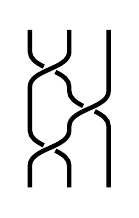
\begin{tikzpicture}
\pic[
  braid/.cd,
  number of strands=3,
  height=.5cm,
  width=.5cm,
  ultra thick,
  gap=0.1,
  name prefix=braid,
] {braid={a_{1}a_2a_1}};
\end{tikzpicture}
\hspace{1cm}
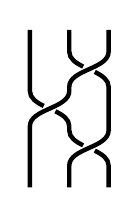
\begin{tikzpicture}
\pic[
  braid/.cd,
  number of strands=3,
  height=.5cm,
  width=.5cm,
  ultra thick,
  gap=0.1,
  name prefix=braid,
] {braid={a_{2}a_1a_2}};
\end{tikzpicture}
\caption{The Yang--Baxter equation.}
\label{fig:braid}
\end{figure}

\index{Braid group}
For $n\geq2$, the \emph{braid group} $\B_n$ is defined as the group with generators $\sigma_1,\dots,\sigma_{n-1}$ and relations
\begin{align*}
    &\sigma_i\sigma_{i+1}\sigma_i=\sigma_{i+1}\sigma_i\sigma_{i+1} && \text{if }1\leq i\leq n-2,\\
    &\sigma_i\sigma_j=\sigma_j\sigma_i && \text{if }|i-j|> 1.
\end{align*}
Let $(X,r)$ be a set-theoretic solution to the YBE. Write $X^n=X\times\cdots\times X$ ($n$-times).  
For $i<n$ let 
$r_{i,i+1}=\id_{X^{i-1}}\times r\times\id_{X^{n-i-1}}\colon X^n\to X^n$.
Then the map $\sigma_i\mapsto r_{i,i+1}$ extends 
to an action of $\B_n$ on $X^n$.

\begin{example}
Let $X$ be a non-empty set. Then $(X,\id)$ is a set-theoretic 
solution to the YBE. 	
\end{example}

\begin{example}
\index{Solution!trivial}
Let $X$ be a non-empty set. Then $(X,r)$, where $r(x,y)=(y,x)$, is a  set-theoretic solution to the YBE. This solution 
is known as the \emph{trivial solution} over the set $X$. 
\end{example}

By convention, we write
\[
r(x,y)=(\sigma_x(y),\tau_y(x)).
\]

\begin{lemma}
    \label{lem:YB}
    Let $X$ be a non-empty set and $r\colon X\times X\to X\times X$ be a bijective map.
    Then $(X,r)$ is a set-theoretic solution to the YBE if and only if 
    \begin{align*}
        &\sigma_x\sigma_y = \sigma_{\sigma_x(y)}\sigma_{\tau_y(x)},&
        &\sigma_{\tau_{\sigma_y(z)}(x)}\tau_z(y)=\tau_{\sigma_{\tau_y(x)}(z)}\sigma_x(y),&
        &\tau_z\tau_y=\tau_{\tau_z(y)}\tau_{\sigma_y(z)}
    \end{align*}
    for all $x,y,z\in X$. 
\end{lemma}

\begin{proof}
    We write $r_1=r\times\id$ and $r_2=\id\times r$. We first compute
    \begin{align*}
        r_1r_2r_1(x,y,z)&=r_1r_2(\sigma_x(y),\tau_y(x),z)
        =r_1(\sigma_x(y),\sigma_{\tau_y(x)}(z),\tau_z\tau_y(x))\\
        &=\left(\sigma_{\sigma_x(y)}\sigma_{\tau_y(x)}(z),\tau_{\sigma_{\tau_y(x)}(z)}\sigma_x(y),\tau_z\tau_y(x)\right).
    \end{align*}
    Then we compute
    \begin{align*}
        r_2r_1r_2(x,y,z)&=r_2r_1(x,\sigma_y(z),\tau_z(y))
        =r_2(\sigma_x\sigma_y(z),\tau_{\sigma_y(z)}(x),\tau_z(y))\\
        &=\left(\sigma_x\sigma_y(z),\sigma_{\tau_{\sigma_y(z)}(x)}\tau_z(y),\tau_{\tau_z(y)}\tau_{\sigma_y(z)}(x)\right)
    \end{align*}
    and the claim follows.    
\end{proof}

If $(X,r)$ is a set-theoretic solution, by definition the map $r\colon X\times X\to X\times X$ is 
invertible. By convention, we write 
 \[
 r^{-1}(x,y)=(\widehat{\sigma}_x(y),\widehat{\tau}_y(x)).
 \]
 Note that this implies that
 \[
 x=\widehat{\sigma}_{\sigma_x(y)}\tau_y(x),\quad
 y=\widehat{\tau}_{\tau_y(x)}\sigma_x(y).
 \]
 It is easy to check that $(X,r^{-1})$ is a set-theoretic solution to the YBE. Thus Lemma~\ref{lem:YB} implies that 
 the following formulas hold:
 \[
 \widehat{\tau}_y\widehat{\tau_x}=\widehat{\tau}_{\tau_y(x)}\widehat{\tau}_{\sigma_x(y)},
 \quad
 \widehat{\sigma}_x\widehat{\sigma_y}=\widehat{\sigma}_{\sigma_x(y)}\widehat{\sigma}_{\tau_y(x)}.
 \]
% Since $r(\tau^{-1}_y(x),y)=(\sigma_{\tau^{-1}_y(x)}(y),x)$, 
% it follows that 
% \[
% \widehat{\tau}_x\sigma_{\tau^{-1}_y(x)}(y)=y.
% \]
% for all $x,y\in X$. Moreover, 
% \[
% x\triangleright y=\tau_x\sigma_{\tau^{-1}_y(x)}(y)=\tau_x\widehat{\tau}^{-1}_x(y)
% \]
% for all $x,y\in X$. 

\begin{example}
Let $X=\{1,2,3,4\}$ and $r(x,y)=(\sigma_x(y),\tau_y(x))$, where
\begin{align*}
&\sigma_1=(132),&&
\sigma_2=(124),&&
\sigma_3=(143),&&
\sigma_4=(234),\\
&\tau_1=(12)(34),&&
\tau_2=(12)(34),&&
\tau_3=(12)(34),&&
\tau_4=(12)(34).
\end{align*}
Then $r$ is invertible with $r^{-1}(x,y)=(\widehat{\sigma}_x(y),\widehat{\tau}_y(x))$ given by
\begin{align*}
&\widehat{\sigma}_1=(12)(34), &&
\widehat{\sigma}_2=(12)(34), &&
\widehat{\sigma}_3=(12)(34), &&
\widehat{\sigma}_4=(12)(34),\\
&\widehat{\tau}_1=(142),&&
\widehat{\tau}_2=(123),&&
\widehat{\tau}_3=(243),&&
\widehat{\tau}_4=(134).
\end{align*}
\end{example}

\begin{definition}
A \emph{homomorphism} between the set-theoretic solutions $(X,r)$ and
$(Y,s)$ is a map $f\colon X\to Y$ such that the diagram 
\[\begin{tikzcd}
	{X\times X} & {X\times X} \\
	{Y\times Y} & {Y\times Y}
	\arrow["r", from=1-1, to=1-2]
	\arrow["{f\times f}"', from=1-1, to=2-1]
	\arrow["{f\times f}", from=1-2, to=2-2]
	\arrow["s"', from=2-1, to=2-2]
\end{tikzcd}
\]
is commutative, that is $s (f\times f)=(f\times f) r$. An \emph{isomorphism} of solutions is a bijective
homomorphism of solutions.
\end{definition}

Since we are interested in studying the combinatorics behind set-theoretic solutions to the YBE,
it makes sense to study the following family of solutions. 

\begin{definition}
\index{Solution!non-degenerate}
We say that a set-theoretic solution $(X,r)$ to the YBE 
is \emph{non-degenerate} if the maps $\sigma_x$ and $\tau_x$ are 
permutations of $X$. 
\end{definition}

By convention, a \emph{solution} we will mean a non-degenerate {\bf set-theoretic} solution to the YBE.

\begin{lemma}
\label{lem:LYZ}
Let $(X,r)$ be a solution. 
\begin{enumerate}
    \item Given $x,u\in X$, there exist unique $y,v\in X$ such that $r(x,y)=(u,v)$. 
    \item Given $y,v\in X$, there exist unique $x,u\in X$ such that $r(x,y)=(u,v)$. 
\end{enumerate}
\end{lemma}

\begin{proof}
    For the first claim take $y=\sigma_x^{-1}(u)$ and $v=\tau_y(x)$. 
    For the second, $x=\tau_y^{-1}(v)$ and $u=\sigma_x(y)$. 
\end{proof}

The bijectivity of $r$ means that any row determines the whole square. Lemma~\ref{lem:LYZ}
means that any column also determines the whole square, see Figure~\ref{fig:braid}.

\begin{figure}
\centering
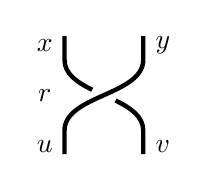
\begin{tikzpicture}
\pic[
  braid/.cd,
  number of strands=2,
  ultra thick,
  gap=0.1,
  name prefix=braid,
] {braid={a_{1}^{-1}}};
\node[] at (-.25,-.12) {$x$};
\node[] at (1.25,-.12) {$y$};
\node[] at (-.25,-1.4) {$u$};
\node[] at (1.25,-1.4) {$v$};
\node[] at (-.25,-.75) {$r$};
\end{tikzpicture}
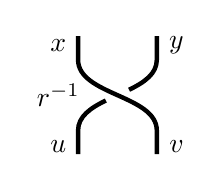
\begin{tikzpicture}
\pic[
  braid/.cd,
  number of strands=2,
  ultra thick,
  gap=0.1,
  name prefix=braid,
] {braid={a_{1}}};
\node[] at (-.25,-.12) {$x$};
\node[] at (1.25,-.12) {$y$};
\node[] at (-.25,-1.4) {$u$};
\node[] at (1.25,-1.4) {$v$};
\node[] at (-.25,-.75) {$r^{-1}$};
\end{tikzpicture}
\caption{Any row or column determines the whole square.}
\label{fig:braid}
\end{figure}

\begin{example}
If the map $(x,y)\mapsto(\sigma_x(y),\tau_y(x))$ satisfies the Yang--Baxter equation, then 
so does $(x,y)\mapsto (\tau_x(y),\sigma_y(x))$. 
\end{example}

\begin{example}
\label{exa:Lyubashenko}
Let $X$ be a non-empty set and $\sigma$ and $\tau$ be 
bijections on $X$ such that $\sigma\circ\tau=\tau\circ\sigma$. Then 
$(X,r)$, where $r(x,y)=(\sigma(y),\tau(x))$, is a non-degenerate solution. 
This is known as the \emph{permutation solution} associated
with permutations $\sigma$ and $\tau$. 
%The solution $(X,r)$ is involutive 
%if and only if $\tau^{-1}=\sigma$. 
\end{example}
%
%\begin{example}
%\label{exa:Wada}
%Let $G$ be a group. Then $(G,r)$, where $r(x,y)=(xy^{-1}x^{-1},xy^2)$, is a solution. 
%\end{example}

\begin{example}
\label{exa:Venkov}
Let $G$ be a group. Then $(G,r)$, where $r(x,y)=(xyx^{-1},x)$, is a solution. 
%It is involutive if and only if $G$ is abelian. 
\end{example}

Now we will prove the main theorem of this chapter. The result
shows an intriguing connection 
between group actions and non-degenerate solutions. It 
was proved by Lu, Yan and Zhu. 

\begin{theorem}
\label{thm:LYZ}
Let $G$ be a group and let $\xi\colon G\times G\to G$, $\xi(x,y)=x\rhd y$,
be a left action of the group $G$ on itself as a set, and 
let $\eta\colon G\times G\to G$, $\eta(x,y)=x\lhd y$, 
be a right action of the group $G$ on itself as a set. If the compatibility condition
\[
uv=(u\rhd v)(u\lhd v)
\]
holds for all $u,v\in G$, then the pair $(G,r)$, where 
\[
r\colon G\times G\to G\times G,\quad
r(u,v)=(u\rhd v,u\lhd v)
\]
is a solution. 
%Moreover, 
%if $r(x,y)=(u,v)$, then 
%\[
%r(x^{-1},y^{-1})=(u^{-1},v^{-1}),
%\quad
%r(x^{-1},u)=(y,v^{-1}),
%\quad
%r(v,y^{-1})=(u^{-1},x).
%\]
\end{theorem}

\begin{proof}
We write $r_1=r\times\id$ and $r_2=\id\times r$. Let
\[
r_1r_2r_1(u,v,w)=(u_1,v_1,w_1),\quad
r_2r_1r_2(u,v,w)=(u_2,v_2,w_2).
\]
The compatibility condition implies that $u_1v_1w_1=u_2v_2w_2$. 
So we need to prove that $u_1=u_2$ and $w_1=w_2$. We note that
\begin{align*}
&u_1=(u\rhd v)\rhd ( (u\lhd v)\rhd w),
&&w_1=(u\lhd v)\lhd w,\\
&u_2=u\rhd (v\rhd w),
&&w_2=(u\lhd (v\rhd w))\lhd (v\lhd w).
\end{align*}
Using the compatibility condition and the fact that $\xi$ is a left action, 
\begin{align*}
    &u_1=((u\rhd v)(u\lhd v))\rhd w=(uv)\rhd w=u\rhd (v\rhd w)=u_2.
\end{align*}
Similarly, since $\eta$ is a right action, 
\[
w_2=u\lhd ((v\rhd w)(v\lhd w))=u\lhd (vw)=(u\lhd v)\lhd w=w_1.
\]

To prove that $r$ is invertible we proceed as follows. 
Write $r(u,v)=(x,y)$, thus $u\rhd v=x$, $u\lhd v=y$ and $uv=xy$. Since 
\begin{align*}
& (y\rhd v^{-1})u=(y\rhd v^{-1})(y\lhd v^{-1})=yv^{-1}=x^{-1}u,
\end{align*}
it follows that $y\rhd v^{-1}=x^{-1}$, i.e. $v^{-1}=y^{-1}\rhd x^{-1}$. Similarly, 
\[
v(u^{-1}\lhd x)=(u^{-1}\rhd x)(u^{-1}\lhd x)=u^{-1}x=vy^{-1}
\]
implies that $u^{-1}=y^{-1}\lhd x^{-1}$. Clearly 
$r^{-1}=\zeta (i\times i) r (i\times i) \zeta$,
is the inverse of $r$, where $\zeta(x,y)=(y,x)$ and $i(x)=x^{-1}$. 
\end{proof}

\begin{proposition}\label{prop:LYZ}
Under the assumptions of Theorem~\ref{thm:LYZ}, 
if $r(x,y)=(u,v)$, then 
\[
r(v^{-1},u^{-1})=(y^{-1},x^{-1}),
\quad
r(x^{-1},u)=(y,v^{-1}),
\quad
r(v,y^{-1})=(u^{-1},x).
\]
\end{proposition}

\begin{proof}
In the proof of Theorem~\ref{thm:LYZ} we found that 
the inverse of the map $r$ is given by $r^{-1}=\zeta (i\times i) r (i\times i) \zeta$,
where $\zeta(x,y)=(y,x)$ and $i(x)=x^{-1}$. Hence 
\[
r^{-1}(y^{-1},x^{-1})=\zeta (i\times i) r (i\times i) \zeta(y^{-1},x^{-1})=\zeta (i\times i) r (x,y)=(v^{-1},u^{-1}).
\]
It follows that $r(v^{-1},u^{-1})=(y^{-1},x^{-1})$.  
To prove the equality $r(x^{-1},u)=(y,v^{-1})$ we proceed as follows. Since $r(x,y)=(u,v)$, it 
follows that $x\rhd y=u$. Then $x^{-1}\rhd u=y$ and
hence $r(x^{-1},u)=(y,z)$ for some $z\in G$. 
Since $xy=uv$ and $x^{-1}u=yz$, it immediately follows that $yz=yv^{-1}$. Then 
$z=v^{-1}$. Similarly one proves $r(v,y^{-1})=(u^{-1},x)$.
\end{proof}
%
%\begin{proposition}
%Under the assumptions of Theorem~\ref{thm:LYZ}, 
%if $r(x,y)=(u,v)$, then 
%\[
%r(x^{-1},y^{-1})=(u^{-1},v^{-1}),
%\quad
%r(x^{-1},u)=(y,v^{-1}),
%\quad
%r(v,y^{-1})=(u^{-1},x).
%\]
%\end{proposition}
%
%\begin{proof}
%In the proof of Theorem~\ref{thm:LYZ} we found that 
%the inverse of the map $r$ is given by $r^{-1}=\zeta (i\times i) r (i\times i) \zeta$,
%where $\zeta(x,y)=(y,x)$ and $i(x)=x^{-1}$. It follows that $r(x^{-1},y^{-1})=(u^{-1},v^{-1})$.  
%To prove the equality $r(x^{-1},u)=(y,v^{-1})$ we proceed as follows. Since $r(x,y)=(u,v)$, it 
%follows that $x\triangleright y=u$. Then $x^{-1}\triangleright u=y$ and
%hence $r(x^{-1},u)=(y,z)$ for some $z\in G$. 
%Since $xy=uv$ and $x^{-1}u=yz$, it follows that $yt=yv^{-1}$. Then 
%$z=v^{-1}$. Similarly one proves $r(v,y^{-1})=(u^{-1},x).$
%\end{proof}

\section{Racks}

\begin{definition}
\label{defn:rack}
\index{Rack}
A \emph{rack} is a pair $(X,\triangleleft)$, 
where $X$ is a non-empty set and 
$X\times X\to X$, $(x,y)\mapsto x\triangleleft y$, is a binary operation on $X$ such that
the maps $\rho_y\colon X\to X$, $x\mapsto x\triangleleft y$, are bijective for all $y\in X$, and 
\begin{equation}
\label{eq:rack}
(x\triangleleft y)\triangleleft z=(x\triangleleft z)\triangleleft (y\triangleleft z)
\end{equation}
for all $x,y,z\in X$.
\end{definition}

Racks are used in low-dimensional topology~\cite{MR3379534}, singularities~\cite{MR975077} 
and in the classification of finite-dimensional pointed Hopf algebras~\cite{MR1994219}.

\begin{example}
\index{Rack!trivial}
    Let $X$ be a set. Then $x\triangleleft y=x$ turns $X$ into a rack. 
    This is the \emph{trivial rack} on $X$. 
\end{example}

\begin{example}
    \index{Rack!dihedral}
    Let $X=\Z/n$. Then $x\triangleleft y=2y-x$ turns $X$ into a rack. This is 
    the \emph{dihedral rack} of size $n$. 
\end{example}

\begin{example}
    \index{Rack!Alexander}
    Let $A$ be an abelian group and $f\in\Aut(A)$. Then 
    \[
    x\triangleleft y=(\id-f)(y)+f(x)
    \]
    turns $A$ into a rack. These racks 
    are known as the \emph{Alexander racks}.
\end{example}

\begin{definition}
    \index{Rack!homomorphism}
    \index{Rack!isomorphism}
    \index{Homomorphism!of racks}
    Let $X$ and $Z$ be racks. 
    A \emph{rack homomorphism} between the racks $X$ and $Z$ is a map $f\colon X\to Z$ such that 
    $f(x\triangleleft y)=f(x)\triangleleft f(y)$ for all $x,y\in X$. 
    An \emph{isomorphism} of racks is a bijective rack homomorphism. 
\end{definition}

For $n\in\N$, let $r(n)$ be the number of isomorphism classes of racks of size
$n$. Some values of $r(n)$ appear in Table~\ref{tab:racks}, see for example~\cite{MR3957904}.  

\begin{table}[H]
\centering
\caption{Enumeration of non-isomorphic racks.}
\begin{tabular}{|c|cccccccccccc|}
\hline
$n$ & 2 & 3 & 4 & 5 & 6 & 7 & 8 & 9 & 10 & 11 & 12 & 13\tabularnewline
\hline
$r(n)$ & 2 & 6 & 19 &74&353 & 2080 & 16023 & 159526 & 2093244 & 36265070 & 836395102 & 25794670618\tabularnewline
\hline
\end{tabular}
\label{tab:racks}
\end{table}

\begin{proposition}
\label{pro:Venkov}
Let $X$ be a non-empty set and $X\times X\to X$, $(x,y)\mapsto x\triangleleft y$ be a binary operation on $X$. Then
$r(x,y)=(y,x\triangleleft y)$ is a solution if and only if $(X,\triangleleft)$ is a rack. 
\end{proposition}

\begin{proof}
The map $r$ satisfies $(r\times\id)(\id\times r)(r\times\id)=(\id\times r)(r\times\id)(\id\times r)$ if and only
if~\eqref{eq:rack} holds for all $x,y,z\in X$. The solution $(X,r)$ is non-degenerate if 
the maps $X\to X$, $x\mapsto x\triangleleft y$, are bijective. 
\end{proof}

The connection between racks and solutions goes deeper than 
the phenomenon appearing in Proposition~\ref{pro:Venkov}. 


\begin{proposition}
    \label{pro:derived}
    Let $(X,r)$ be a solution. Then 
    \begin{equation}
    \label{eq:derived}
    x\triangleleft y=\sigma_y\tau_{\sigma_x^{-1}(y)}(x)=\sigma_y\widehat{\sigma}^{-1}_y(x)
    \end{equation}
    turns $X$ into a rack and each $\sigma_x$ is a rack homomorphism. 
    Moreover, $(X,r)$ is involutive if and only if the rack $(X,\triangleleft)$ is trivial. 
\end{proposition}

\begin{proof}
    Since $r(x,\sigma_x^{-1}(y))=(y,\tau_{\sigma_x^{-1}(y)}(x))$, 
    it follows that 
    $\widehat{\sigma}_y^{-1}(x)=\tau_{\sigma_x^{-1}(y)}(x)$ 
    for all $x,y\in X$. Hence the second equality of~\eqref{eq:derived} holds. {\bf Therefore the maps $X\to X,\, x\mapsto x\triangleleft y$ are bijective}.
    
    {\bf Now we shall show that}
    \begin{equation}\label{eq:rackhom}
    \sigma_x(y)\triangleleft \sigma_x\sigma_y(z)=\sigma_x(y\triangleleft\sigma_y(z))
    \end{equation}
    for all $x,y\in X$. Write $r(x,y)=(u,v)$. On the one hand, by 
    Lemma~\ref{lem:YB}, 
    \begin{align*}
        \sigma_x(y)\triangleleft \sigma_x\sigma_y(z)
        &=u\triangleleft \sigma_u\sigma_v(z)
        =\sigma_{\sigma_u\sigma_v(z)}\tau_{\sigma_{\tau_y(x)}(z)}\sigma_x(y)
        =\sigma_{\sigma_x\sigma_y(z)}\sigma_{\tau_{\sigma_y(z)}(x)}\tau_z(y).
    \end{align*}
    On the other hand, 
    \begin{align*}
        \sigma_x(y\triangleleft\sigma_y(z)) 
        &=\sigma_x\sigma_{\sigma_y(z)}\tau_z(y)
        =\sigma_{\sigma_x\sigma_y(z)}\sigma_{\tau_{\sigma_y(z)}(x)}\tau_z(y).
    \end{align*}
{\bf Therefore, (\ref{eq:rackhom}) follows.}
    
    By Proposition~\ref{pro:Venkov}, in order to prove that $(X,\triangleright)$ is a rack it is enough to show that
    $s(x,y)=(y,x\triangleleft y)$ satisfies the YBE. For that purpose, we demonstrate that 
    the map $J\colon X^3\to X^3$, $J(x,y,z)=(x,\sigma_x(y),\sigma_x\sigma_y(z))$ 
    is invertible and 
    satisfies 
    \[
    (\id\times s)\circ J=J\circ(\id\times r),
    \quad
    (s\times\id)\circ J=J\circ(r\times\id).
    \]
    {\bf One can easily check that the} map $(x,y,z)\mapsto (x,\sigma_x^{-1}(y),\sigma_{\sigma_x^{-1}(y)}^{-1}\sigma_x^{-1}(z))$ is the inverse of $J$. 

    {\bf By (\ref{eq:rackhom}),} 
    \begin{align*}
    \sigma_x(y)\triangleleft \sigma_x\sigma_y(z)
    &=\sigma_x(y\triangleleft \sigma_y(z))
    =\sigma_x\sigma_{\sigma_y(z)}\tau_{\sigma_y^{-1}\sigma_y(z)}(y)
    =\sigma_x\sigma_{\sigma_y(z)}\tau_z(y)
    \end{align*}
    Then it follows that 
    \begin{align*}
        (\id\times s)J(x,y,z)
        &=(\id\times s)(x,\sigma_x(y),\sigma_x\sigma_y(z))\\
        &=(x,\sigma_x\sigma_y(z),\sigma_x(y)\triangleleft \sigma_x\sigma_y(z))\\
        &=(x,\sigma_x\sigma_y(z),\sigma_x\sigma_{\sigma_y(z)}\tau_z(y))\\
        &=J(x,\sigma_y(z),\tau_z(y))\\
        &=J(\id\times r)(x,y,z).
    \end{align*}
    Similarly one proves that $(s\times\id)\circ J=J\circ (r\times\id)$.  
    This implies that $(X,s)$ is a solution and 
    hence $(X,\triangleleft)$ is a rack by Proposition~\ref{pro:Venkov}. 

    If $(X,r)$ is involutive, 
    then $x\triangleleft\sigma_x(y)=\sigma_{\sigma_x(y)}\tau_y(x)=x$ by~\eqref{eq:involutive}. 
    Conversely, if $x\triangleleft y=x$ for all $x,y\in X$,
    then $r$ is involutive, as 
    \[
    r^2(x,\sigma_x^{-1}(y))=r(y,\sigma_y^{-1}(x))=(x,\sigma_x^{-1}(y)).\qedhere
    \]
\end{proof}

%\begin{definition}
\index{Solution!derived rack}
The rack constructed in Proposition~\ref{pro:derived} is 
known as the \emph{derived rack} of $(X,r)$. 
%\end{definition}
There is a dual version of the derived rack:

\begin{proposition}
    \label{pro:derived_dual}
    Let $(X,r)$ be a solution. Then 
    \[
    x\blacktriangleleft y=\tau_y\sigma_{\tau_x^{-1}(y)}(x)=\tau_y\widehat{\tau}^{-1}_y(x)
    \]
    turns $X$ into a rack and each $\tau_x$ is a rack homomorphism. 
\end{proposition}

\begin{proof}
    Since $(X,r)$ is a solution, then so is $(X,r_0)$, where 
    $r_0(x,y)=(\tau_x(y),\sigma_y(x))$. Then the claim follows 
    from Proposition~\ref{pro:derived} applied to 
    the solution $(X,r_0)$.
\end{proof}

\index{Solution!dual derived rack}
{\bf The rack constructed in Proposition~\ref{pro:derived_dual} is 
known as the \emph{dual derived rack} of $(X,r)$.} 


In general, the racks constructed in Propositions~\ref{pro:derived} 
and~\ref{pro:derived_dual} are different:

\begin{example}
Let $X=\{1,\dots,5\}$ and $(X,r)$ be the solution given by
\begin{align*}
&\sigma_1=\id, && \sigma_2=\id, && \sigma_3=\id, && \sigma_4=(13)(45), &&\sigma_5=(12)(45),\\
&\tau_1=\id, && \tau_2=\id, && \tau_3=\id, && \tau_4=(23)(45), &&\tau_5=(23)(45).
\end{align*}
On the one hand the derived rack of $(X,r)$ is given by the permutations 
\begin{align*}
&\sigma_1\widehat{\sigma}_1^{-1}=\sigma_2\widehat{\sigma}_2^{-1}=\sigma_3\widehat{\sigma}_3^{-1}=\id,
&&\sigma_4\widehat{\sigma}_4^{-1}=(132),
&&\sigma_5\widehat{\sigma}_5^{-1}=(123).
\end{align*}
On the other hand, the dual derived rack by 
\begin{align*}
&\tau_1\widehat{\tau}_1^{-1}=\tau_2\widehat{\tau}_2^{-1}=\tau_3\widehat{\tau}_3^{-1}=\id,
&&\tau_4\widehat{\tau}_4^{-1}=(123),
&&\tau_5\widehat{\tau}_5^{-1}=(132).
\end{align*}
% [ [ (), (), (), (1,3)(4,5), (1,2)(4,5) ], [ (), (), (), (2,3)(4,5), (2,3)(4,5) ] ]
%[ [ (), (), (), (2,3)(4,5), (2,3)(4,5) ], [ (), (), (), (1,3)(4,5), (1,2)(4,5) ] ]
% [ (), (), (), (1,3,2), (1,2,3) ]
% [ (), (), (), (1,2,3), (1,3,2) ]
\end{example}

We now prove that the racks 
of Propositions~\ref{pro:derived} 
and~\ref{pro:derived_dual} are isomorphic. 
We shall need a lemma. 



\begin{lemma}
\label{lem:T_invertible}
Let $(X,r)$ be a solution. 
The map $T\colon X\to X$, $x\mapsto\sigma_x^{-1}(x)$, is invertible with
inverse $U\colon X\to X$, $x\mapsto\tau^{-1}_x(x\blacktriangleleft x)$. 
\end{lemma}

\begin{proof}
Let $x\in X$ and $y=U(x)=\tau^{-1}_x(x\blacktriangleleft x)$. 
Then $\tau_x(y)=x\blacktriangleleft x=\tau_x\widehat{\tau}^{-1}_x(x)$ and hence
$y=\widehat{\tau}^{-1}_x(x)$. Then $\widehat{\tau}_x(y)=x$ and 
\[
r^{-1}(y,x)=(\widehat{\sigma}_y(x),x)=(z,x),
\]
where $z\in X$ is such that $\sigma_z(x)=y$. By Lemma~\ref{lem:YB}, $\sigma_y=\sigma_z$. Then 
it follows that $x=\sigma^{-1}_y(y)=T(y)$. Therefore $y=U(x)=U(T(y))$.

To prove that $T(U(x))=x$, first note that 
\[
r(\tau^{-1}_x(x),x)=(\sigma_{\tau^{-1}_x(x)}(x),x)
\]
and Lemma~\ref{lem:YB} imply that $\sigma_{\tau^{-1}_x(x)}=\sigma_{\sigma_{\tau^{-1}_x(x)}(x)}$. Now
\begin{align*}
T(U(x))&=T(\tau^{-1}_x(x\blacktriangleleft x))=T(\sigma_{\tau^{-1}_x(x)}(x))\\
&=\sigma^{-1}_{\sigma_{\tau^{-1}_x(x)}(x)}\sigma_{\tau^{-1}_x(x)}(x)
=\sigma^{-1}_{\tau^{-1}_x(x)}\sigma_{\tau^{-1}_x(x)}(x)=x.\qedhere
\end{align*}
\end{proof}

There is {\bf a} version of Proposition~\ref{pro:T} for arbitrary solutions. 
A similar result appears in Exercise~\ref{prob:variationT}.



\begin{proposition}
    Let $(X,r)$ be a solution. Then $T\colon X\to X$, $x\mapsto\sigma_x^{-1}(x)$, is a bijective
    map such that 
    \[
      T\circ\tau_y=\widehat{\sigma}^{-1}_y\circ T,
      \quad
      T\circ \widehat{\tau_y}=\sigma^{-1}_{y}\circ T
    \]
    and $T(x\blacktriangleleft y)=T(x)\triangleleft T(y)$ for all $x,y\in X$. 
\end{proposition}

\begin{proof}
    Lemma~\ref{lem:T_invertible} proves that $T$ is bijective. 
    We now compute 
    \begin{align*}
        T\tau_y(x) &= 
        \sigma^{-1}_{\tau_y(x)}\tau_y(x)
        =\sigma^{-1}_{\tau_y(x)}\sigma^{-1}_{\sigma_x(y)}\sigma_{\sigma_x(y)}\tau_y(x)\\
        &=\sigma^{-1}_y\sigma^{-1}_x\sigma_{\sigma_x(y)}\tau_y(x)
        =\sigma^{-1}_y\sigma_x^{-1}(x\triangleleft\sigma_x(y))
        =\sigma^{-1}_y(T(x)\triangleleft y)
        =\widehat{\sigma}^{-1}_yT(x).
    \end{align*}

    Since $\widehat{\tau}_y(x)=\sigma^{-1}_{\widehat{\sigma}_x(y)}(x)$, Lemma~\ref{lem:YB} implies that 
    \begin{align*}
        T\widehat{\tau_y}(x) 
        &=\sigma^{-1}_{\widehat{\tau}_y(x)}\widehat{\tau}_y(x)
        =\sigma^{-1}_{\widehat{\tau}_y(x)}\sigma^{-1}_{\widehat{\sigma}_x(y)}(x)
        =\sigma^{-1}_{y}\sigma^{-1}_{x}(x)
        =\sigma^{-1}_{y}T(x).
    \end{align*}
    These formulas imply that
    \begin{equation}
        \label{eq:T_rack}
        T\circ\tau_y\circ\widehat{\tau}_y^{-1}
        =\widehat{\sigma}^{-1}_y\circ T\circ \widehat{\tau}^{-1}_y
        =\widehat{\sigma}^{-1}_y\circ \sigma_y\circ T.
    \end{equation}

    We evaluate Equality~\eqref{eq:T_rack} on $X$. On the one hand, 
    $T(x\blacktriangleleft y)=T\tau_y\widehat{\tau_y}^{-1}(x)$.
    On the other hand,
    \begin{align*}
        \widehat{\sigma}_y^{-1}\sigma_yT(x)
        &=\sigma_y^{-1}\sigma_y\widehat{\sigma}_y^{-1}\sigma_yT(x)
        =\sigma_y^{-1}(\sigma_yT(x)\triangleleft y)=T(x)\triangleleft T(y).\qedhere
    \end{align*}
\end{proof}


%If $(X,r)$ is a solution, the map $r\colon X\times X\to X\times X$ is invertible. Write 
% \[
% r^{-1}(x,y)=(\widehat{\sigma}_x(y),\widehat{\tau}_y(x)).
% \]
% Since $(X,r^{-1})$ is a solution, Lemma~\ref{lem:YB} implies that 
% the following formulas hold:
% \[
% \widehat{\tau}_y\widehat{\tau_x}=\widehat{\tau}_{\tau_y(x)}\widehat{\tau}_{\sigma_x(y)},
% \quad
% \widehat{\sigma}_x\widehat{\sigma_y}=\widehat{\sigma}_{\sigma_x(y)}\widehat{\sigma}_{\tau_y(x)}.
% \]
% Since $r(\tau^{-1}_y(x),y)=(\sigma_{\tau^{-1}_y(x)}(y),x)$, 
% it follows that 
% \[
% \widehat{\tau}_x\sigma_{\tau^{-1}_y(x)}(y)=y.
% \]
% for all $x,y\in X$. Moreover, 
% \[
% x\triangleright y=\tau_x\sigma_{\tau^{-1}_y(x)}(y)=\tau_x\widehat{\tau}^{-1}_x(y)
% \]
% for all $x,y\in X$. 

%We first need a lemma. 

% \begin{proposition}
%     Let $(X,r)$ be a solution and let $(X,\triangleright)$ be its derived rack. 
%     Then 
%     \[
%     T\circ \sigma_x=\tau_x^{-1}\circ\rho_x\circ T
%     \]
%     for all $x\in X$, where $T\colon X\to X$, $T(y)=\tau_y^{-1}(y)$, and 
%     $\rho_x\colon X\to X$, $\rho_x(y)=x\triangleright y$.
% \end{proposition}

% \begin{proof}
% By using Lemma~\ref{lem:YB} we compute 
% \begin{align*}
%     T\sigma_x(y) &= \tau^{-1}_{\sigma_x(y)}\sigma_x(y)
%     =\tau^{-1}_{\sigma_x(y)}(\tau^{-1}_{\tau_y(x)}(\tau_y(x)\triangleright y))\\
%     &=\tau^{-1}_{\sigma_x(y)}\tau^{-1}_{\tau_y(x)}(\tau_y(x)\triangleright y))\\
%     &=\tau^{-1}_{x}\tau^{-1}_{y}(\tau_y(x)\triangleright y))\\
%     &=\tau^{-1}_{x}(x\triangleright T(y)).\qedhere 
% \end{align*}
% \end{proof}

% \begin{proposition}
% \label{pro:T_general}
% Let $(X,r)$ be a solution. 
% The map $T\colon X\to X$, $x\mapsto\sigma_{\tau_x^{-1}(x)}(x)$, is invertible with
% inverse $U\colon X\to X$, $x\mapsto\sigma^{-1}_x(x)$. 
% \end{proposition}

% \begin{proof}
% Let $(X,\triangleright)$ be the derived rack of $(X,r)$. Then 
% $T(x)=\tau_x^{-1}(x\triangleright x)$. Since 
% $r(\tau_z^{-1}(z),z)=(\sigma_{\tau^{-1}_z(z)}(z),z)$, 
% \begin{equation}
%     \label{eq:Ttrick}
%     \sigma_{\tau^{-1}_z(z)}\circ\sigma_z=\sigma_{\sigma_{\tau^{-1}_z(z)}(z)}\circ\sigma_z
% \end{equation}
% holds for all $z\in X$ by 
% Lemma~\ref{lem:YB}. On the one hand, 
% \begin{align*}
%     U(T(x)) 
%     &= U(\sigma_{\tau^{-1}_x(x)}(x))
%     =\sigma^{-1}_{\sigma_{\tau^{-1}_x(x)}(x)}\sigma_{\tau^{-1}_x(x)}(x)=x
% \end{align*}
% because $\sigma_{\tau^{-1}_x(x)}=\sigma_{\sigma_{\tau^{-1}_x(x)}(x)}$ by~\eqref{eq:Ttrick}. 

% Now let $x,y\in X$ be such that $U(x)=y$. Since $r^{-1}(\sigma_x(y),\tau_y(x))=(x,y)$, 
% it follows that $\widehat{\tau}_{\tau_y(x)}\sigma_x(y)=y$ and that 
% $\widehat{\tau}_{\tau_y(x)}=\widehat{\tau_y}$. Then
% \[
% \widehat{\tau}_y(x)=\widehat{\tau}_{\tau_y(x)}(x)=\widehat{\tau}_{\tau_y(x)}\sigma_x(y)=y
% \]
% and hence $\widehat{\tau}^{-1}_y(y)=x$. Now $y\triangleright y=\tau_y\widehat{\tau}^{-1}_y(y)=\tau_y(x)$ and therefore
% \[
% T(y)=\tau_y^{-1}(y\triangleright y)=x.\qedhere
% \]
% \end{proof}

As it happens in the involutive case, there is a nice combinatorial structure that describes  
a solution. 

\begin{definition}
\index{Skew cycle set}
\index{Skew cycle set!non-degenerate}
\label{defn:skewCS}
A \emph{skew cycle set} is a triple $(X,\triangleleft,\cdot)$, where $X$ is a non-empty set, 
$(X,\triangleleft)$ is a rack and
$X\times X\to X$, $(x,y)\mapsto x\cdot y$, is a binary operation on $X$ such that the maps 
$X\to X$, $y\mapsto x\cdot y$, are bijective rack homomorphisms, and 
\begin{equation}
\label{eq:skew_CS}
(x\cdot y)\cdot (x\cdot z)=(y\cdot (x\triangleleft y))\cdot (y\cdot z)
\end{equation}
for all $x,y,z\in X$. A skew cycle set $(X,\triangleleft,\cdot)$ is said to be 
non-degenerate if the map $X\times X$, $x\mapsto x\cdot x$, is bijective.
\end{definition}

\framebox{FIXME}

\begin{definition}
\index{Homomorphism!of skew cycle sets}
Let $X$ and $Z$ be skew cycle sets. 
A \emph{homomorphism} between the {\bf skew} cycle sets $X$ and $Z$ is a 
map $f\colon X\to Z$ such that $f(x\cdot y)=f(x)\cdot f(y)$ {\bf and $f(x\triangleleft y)=f(x)\triangleleft f(y)$,} for all $x,y\in X$. An \emph{isomorphism} of {\bf skew} cycle sets
is a bijective homomorphism of {\bf skew} cycle sets. 
\end{definition}

%Cycle sets and cycle set homomorphisms form a category. 
%It is possible to prove that the category of 
%solutions is equivalent to the category of cycle sets, 
%see Exercise~\ref{prob:cycle_sets}. 


Theorem~\ref{thm:CS} can be generalized to arbitrary solutions.

\begin{theorem}
\label{thm:skewCS}
There exists a bijective correspondence between solutions 
and non-degenerate skew cycle sets. 
\end{theorem}

\begin{proof}
Let $(X,r)$ be a solution and $(X,\triangleleft)$ its derived rack. We will prove that 
the operation $x\cdot y=\sigma_x^{-1}(y)$ turns $(X,\triangleleft)$ into a skew cycle set.
By Proposition~\ref{pro:derived}, 
the 
maps $X\to X$, $y\mapsto x\cdot y$, are bijective rack homomorphisms. 

On the one hand, since $r(x,\sigma_x^{-1}(y))=(y,\tau_{\sigma_x^{-1}(y)}(x))$, 
\begin{align*}
(x\cdot y)\cdot (x\cdot z)
&=\sigma_x^{-1}(y)\cdot\sigma_x^{-1}(z)
=\sigma_{\sigma_x^{-1}(y)}^{-1}\sigma_x^{-1}(z)\\
&=\left(\sigma_x\circ\sigma_{\sigma_x^{-1}(y)}\right)^{-1}(z)
=\left(\sigma_y\circ\sigma_{\tau_{\sigma_x^{-1}(y)}(x)}\right)^{-1}(z).
\end{align*}
On the other hand, 
\begin{align*}
(y\cdot (x\triangleleft y))\cdot (y\cdot z)
&=\sigma_y^{-1}(\sigma_y\tau_{\sigma_x^{-1}(y)}(x))\cdot\sigma_y^{-1}(z)\\
&=\sigma^{-1}_{\tau_{\sigma_x^{-1}(y)}(x)}\sigma_y^{-1}(z)
=\left(\sigma_y\circ\sigma_{\tau_{\sigma^{-1}_x(y)}(x)}\right)^{-1}(z).
\end{align*}

{\bf Therefore $(X,\triangleleft ,\cdot)$ is a skew cycle set. Furthermore, by Lemma \ref{lem:T_invertible}, this skew cycle set is non-degenerate.}

Now we prove the converse statement. {\bf Let $(X,\triangleleft,\cdot)$ be a non-degenerate skew cycle set.} 
For $x,y\in X$ let 
\[
\sigma_x(y)=x*y,
\quad
\tau_y(x)=\sigma_{\sigma_x(y)}^{-1}(x\triangleleft\sigma_x(y)), 
\]
where $x*y=z$ if and only if $x\cdot z=y$. 
Since $X$ is a skew cycle set, each $\sigma_x$ is bijective. Let us prove that the $\tau_x$ are bijective. 
Equality~\eqref{eq:skew_CS} with $y=\sigma_x(z)$ implies that
\begin{equation}\label{eq:solskew}
\sigma_z^{-1}\sigma_x^{-1}=\sigma^{-1}_{\sigma_x^{-1}(y)}\sigma_x^{-1}
=\sigma^{-1}_{\sigma_y^{-1}(x\triangleleft y)}\sigma_y^{-1}
=\sigma^{-1}_{\sigma^{-1}_{\sigma_x(z)}(x\triangleleft\sigma_x(z))}\sigma^{-1}_{\sigma_x(z)}
=\sigma^{-1}_{\tau_z(x)}\sigma^{-1}_{\sigma_x(z)}
\end{equation}
for all $x,z\in X$. 
Since each $\sigma_x$ is a rack homomorphism, 
\[
\tau_y(x)=\sigma^{-1}_{\sigma_x(y)}(x\triangleleft\sigma_x(y))
=\sigma^{-1}_{\sigma_x(y)}\sigma_x(\sigma^{-1}_x(x)\triangleleft y)
=\sigma_{\tau_y(x)}\sigma_y^{-1}(\sigma_x^{-1}(x)\triangleleft y).
\]
Therefore $T\circ\tau_y=\sigma_y^{-1}\circ\rho_y\circ T$, where $T\colon X\to X$, $T(x)=x\cdot x$ 
and $\rho_y\colon X\to X$, $\rho_y(x)=x\triangleleft y$ are bijective maps. In particular, 
$\tau_y$ is bijective for all $y\in X$. 

Let $r\colon X\times X\to X\times X$ be the map defined by $r(x,y)=(\sigma_x(y),\tau_y(x))$, for all $x,y\in X$. 
Now we prove that $(X,r)$ is a solution. Let $s\colon X\times X\to X\times X$ be the map defined by $s(x,y)=(y,x\triangleleft y)$. By Proposition \ref{pro:Venkov}, $(X,s)$ is a solution. As in the proof of Proposition \ref{pro:derived}, The map $J\colon X^3\to X^3$, $J(x,y,z)=(x,\sigma_x(y),\sigma_x\sigma_y(z))$ is invertible and satisfies that 
$$(\id\times s)\circ J=J\circ (\id\times r),$$
because the $\sigma_x$ are rack homomorphisms. Furthermore, by (\ref{eq:solskew}) we have that
\begin{align*}
	(s\times \id)J(x,y,z)&=(s\times \id)(x,\sigma_x(y),\sigma_x\sigma_y(z))\\
	&=(\sigma_x(y),x\triangleleft \sigma_x(y),\sigma_x\sigma_y(z))\\
	&=(\sigma_x(y), \sigma_{\sigma_x(y)}\tau_y(x),\sigma_{\sigma_x(y)}\sigma_{\tau_y(x)}(z))\\
	&=J(\sigma_x(y),\tau_y(x),z)\\
	&=J(r\times \id)(x,y,z).
\end{align*}
Therefore $(X,r)$ is a solution.

Let $(X,\triangleleft,\cdot)$ be a non-degenerate skew cycle set. Let $\varphi(X,\triangleleft,\cdot)=(X,r)$, where
$r(x,y)=(x*y,(x*y)\cdot(x\triangleleft (x*y)))$, where $x*y=z$ if and only if $y=x\cdot z$. We have seen that $(X,r)$ is a solution.

For every solution $(X,r)$ we define $\psi(X,r)=(X,\triangleleft,\cdot)$, where $x\triangleleft y=\sigma_y\tau_{\sigma_x^{-1}(y)}(x)$ and $x\cdot y=\sigma_x^{-1}(y)$. We have seen that $(X,\triangleleft,\cdot)$ is a non-degenerate skew cycle set.

It is easy to check that $\psi(\varphi(X,\triangleleft,\cdot))=(X,\triangleleft,\cdot)$, for every non-degenerate skew cycle set $(X,\triangleleft,\cdot)$, and $\varphi(\psi(X,r))=(X,r)$, for every solution $(X,r)$.
\end{proof}

Theorem~\ref{thm:skewCS} can be used to construct small solutions, see Table~\ref{tab:non_involutive}.

\begin{table}[H]
\centering
\caption{Enumeration of non-involutive solutions.}
\begin{tabular}{|c|ccccccc|}
\hline
$n$ & 2 & 3 & 4 & 5 & 6 & 7 & 8\tabularnewline
\hline
$s(n)$ & 2 & 21 & 253 & 3519 & 100071 & 4602720 & 422449480\tabularnewline
\hline
\end{tabular}
\label{tab:non_involutive}
\end{table}

\section*{B}

\index{Quandle}
An interesting family of racks is that that of quandles. A \textbf{quandle} is a rack $(X,\triangleleft)$ 
such that $x\triangleleft x=x$ for all $x\in X$.

{\bf (Ferran: ¿Tienes alguna idea de c\'omo desarrollar el tema?)} 



% \begin{prob}
%     \label{prob:Venkov}
%     Let $X$ be a set and $X\times X\to X$, $(x,y)\to x\triangleright y$. Prove that 
%     the pair $(X,s)$, where
%     $s(x,y)=(x\triangleright y,x)$, is a solution if and only if $(X,\triangleright)$ is a rack. 
%     Prove that
% \end{prob}

\section{Involutive solutions}

We now go back to study solutions to the YBE and discuss the intriguing interplay
between radical rings and involutive solutions. 

\begin{definition}
	\index{Solution!involutive}
	A solution $(X,r)$ is said to be \emph{involutive} if $r^2=\id$. 
\end{definition}

\index{Symmetric group}
For $n\geq2$, the \emph{symmetric group} $\Sym_n$ can be presented 
as the group with generators $\sigma_1,\dots,\sigma_{n-1}$ and relations
\begin{align*}
	&\sigma_i\sigma_{i+1}\sigma_i=\sigma_{i+1}\sigma_i\sigma_{i+1} && \text{if }1\leq i\leq n-2,\\
	&\sigma_i\sigma_j=\sigma_j\sigma_i && \text{if }|i-j|> 1,\\
	&\sigma_i^2=1 && \text{for all $i\in\{1,\dots,n-1\}$}.
\end{align*}
Let $(X,r)$ be an involutive solution. 
Then the map $\sigma_i\mapsto r_{i,i+1}=\id_{X^{i-1}}\times r\times\id_{X^{n-i-1}}$ extends 
to an action of $\Sym_n$ on $X^n$.

\begin{example}
	Let $X$ be a non-empty set and $\sigma$ be a bijection on $X$. Then 
	$(X,r)$, where $r(x,y)=(\sigma(y),\sigma^{-1}(x))$, is an involutive solution. 
\end{example}

\index{Jacobson!radical ring}
\index{Radical ring}
We now present a very important family of involutive solutions. 
These examples show an intriguing connection between the YBE and the 
theory of non-commutative rings. 


% In any ring $R$ the \emph{circle operation} 
% \[
% x\circ y=x+xy+y
% \]
% is always associative and such that $x\circ 0=0\circ x=x$ for all $x\in R$. 
% A non-unital ring (or \emph{ring}, for short) 
% $R$ is said to be a \emph{radical ring} if $(R,\circ)$ is a group. 
% In this case, following Jacobson's notation, the inverse of 
% an element $x$ with respect to the circle operation is denoted by $x'$. 


\begin{example}
	Let $p$ be a prime and let $A=\Z/(p^2)=\Z/p^2\Z$ be the cylic additive group of order $p^2$. 
	Then $A$ with a new multiplication $*$ defined by $a*b=pab$ is a radical ring. In this case, $x\circ y=x+y+pxy$, and $x'=-x+px^2$. 
\end{example}

\begin{example}
	Let $n$ be an integer such that $n>1$. Let $A=\left\{\frac{nx}{ny+1}:x,y\in\Z\right\}\subseteq \Q$. Note that A is a subring without unity of the field $\Q$. In fact $A$ is a radical ring. A straightforward computation shows that 
	\[
	\left(\frac{nx}{ny+1}\right)'=\frac{-nx}{n(x+y)+1}.
	\]
\end{example}

The following fundamental family of solutions appears in~\cite{MR2278047}. 
It turns out to be fundamental in the study of 
set-theoretic solutions to the YBE. 

\begin{proposition}
	\label{pro:Rump}
	Let $R$ be a radical ring. Then $(R,r)$, where 
	\[
	r(x,y)=( -x+x\circ y,(-x+x\circ y)'\circ x\circ y)
	\]
	is an involutive solution.
\end{proposition}

The proposition can demonstrated using Theorem~\ref{thm:LYZ}, 
see Exercise~\ref{prob:Rump}. 
We will prove a stronger result in Theorem~\ref{thm:YB}. 

Note that if $(X,r)$ is an  involutive solution, then 
\[
(x,y)=r^2(x,y)=r(\sigma_x(y),\tau_y(x))=(\sigma_{\sigma_x(y)}\tau_y(x),\tau_{\tau_y(x)}\sigma_x(y)).
\]
Hence 
\begin{equation}
	\label{eq:involutive}
	\tau_y(x)=\sigma_{\sigma_x(y)}^{-1}(x),
	\quad
	\sigma_x(y)=\tau_{\tau_y(x)}^{-1}(y)
\end{equation}
for all $x,y\in X$. Thus for involutive solutions
it is enough to know $\{\sigma_x:x\in X\}$, as from this we obtain the
set $\{\tau_x:x\in X\}$. 


\begin{proposition}
	\label{pro:T}
	Let $(X,r)$ be an involutive solution. 
	Then the map $T\colon X\to X$, $x\mapsto\sigma_x^{-1}(x)$, is 
	invertible with inverse $T^{-1}(y)=\tau^{-1}_y(y)$ and 
	\[
	T^{-1}\circ\sigma_x^{-1}\circ T=\tau_x
	\]
	for all $x\in X$. 
\end{proposition}

\begin{proof}
	Let $U(x)=\tau_x^{-1}(x)$. Since $r$ is involutive, 
	\[
	(U(x),x)=r^2(U(x),x)=r(\sigma_{U(x)}(x),x)=(\sigma_{\sigma_{U(x)}(x)}(x),\tau_x\sigma_{U(x)}(x)).
	\]
	The second coordinate can be written as $U(x)=\sigma_{U(x)}(x)$. This 
	implies that 
	\[
	T(U(x))=\sigma^{-1}_{U(x)}(U(x))=x.
	\]
	Similarly one obtains $U(T(x))=x$. 
	
	Since $(X,r)$ is a solution, Lemma~\ref{lem:YB} implies that 
	$\sigma_x\sigma_y=\sigma_{\sigma_x(y)}\sigma_{\tau_y(x)}$
	%$\tau_{\tau_y(x)}\circ\tau_{\sigma_x(y)}=\tau_y\circ\tau_x$ 
	holds for all $x,y\in X$. Then  
	\[
	\sigma_y^{-1}T(x)
	=\sigma_y^{-1}\sigma_x^{-1}(x)
	=\sigma^{-1}_{\tau_y(x)}\sigma^{-1}_{\sigma_x(y)}(x)
	=\sigma^{-1}_{\tau_y(x)}\tau_y(x)
	=T\tau_y(x)
	\]
	for all $y\in X$, by Equality~\eqref{eq:involutive}.
\end{proof}



\begin{definition}
	\index{Cycle set}
	\index{Cycle set!non-degenerate}
	A \emph{cycle set} is a pair $(X,\cdot)$, where $X$ is a non-empty 
	set provided with a binary operation $X\times X\to X$, $(x,y)\mapsto x\cdot y$, 
	such that 
	\begin{equation}
		\label{eq:cycle_set}
		(x\cdot y)\cdot (x\cdot z)=(y\cdot x)\cdot (y\cdot z)
	\end{equation}
	holds for all $x,y,z\in X$ and each map $\varphi_x\colon X\to X$, $y\mapsto x\cdot y$, is bijective. 
	A cycle set $(X,\cdot)$ is said to be \emph{non-degenerate} 
	if the map $X\to X$, $x\mapsto x\cdot x$, is bijective. 
\end{definition}

\begin{definition}
	\index{Homomorphism!of cycle sets}
	Let $X$ and $Z$ be cycle sets. 
	A \emph{homomorphism} between the cycle sets $X$ and $Z$ is a 
	map $f\colon X\to Z$ such that $f(x\cdot y)=f(x)\cdot f(y)$ for all $x,y\in X$. An \emph{isomorphism} of cycle sets
	is a bijective homomorphism of cycle sets. 
\end{definition}

%Cycle sets and cycle set homomorphisms form a category. 
%It is possible to prove that the category of 
%solutions is equivalent to the category of cycle sets, 
%see Exercise~\ref{prob:cycle_sets}. 

% \framebox{Exercise!}

% \begin{lemma}
% \label{lem:T_forCS}
% If $X$ is a cycle set, then $x\cdot (y\cdot y)=((y*x)\cdot y)\cdot ((y*x)\cdot y)$, where
% $y*x=z$ if and only if $y\cdot z=x$. 
% \end{lemma}

% \begin{proof}
%     Since the operation $x\mapsto y\cdot x$ is bijective, we can write $x=y\cdot (y*x)$. Then, using~\eqref{eq:cycle_set}, 
%     $x\cdot (y\cdot y)=(y\cdot (y*x))\cdot (y\cdot y)=((y*x)\cdot y)\cdot (y*x)\cdot y)$.
% \end{proof}

\begin{theorem}
	\label{thm:CS}
	There exists a bijective correspondence between non-isomorphic involutive solutions 
	and non-isomorphic non-degenerate cycle sets. 
\end{theorem}



% \begin{proof}
%     Let us assume first that $r(x,y)=(\sigma_x(y),\tau_y(x))$ is an involutive solution. 
%     We want to prove that the operation
%     $x\cdot y=\sigma_x^{-1}(y)$ turns the set $X$ into a non-degenerate cycle set. 
%     It is clear that the maps $y\mapsto x\cdot y=\sigma_x^{-1}(y)$ are invertible. 
%     By Proposition~\ref{pro:T}, the operation $x\mapsto x\cdot x$ is bijective. \framebox{!}
%     Since $r(\tau^{-1}_y(x),y)=(\sigma_{\tau^{-1}_y(x)}(y),x)$, Lemma~\ref{lem:YB} implies that
%     \[
%     \tau_x\circ\tau_{\sigma_{\tau^{-1}_y(x)}(y)}=\tau_y\circ\tau_{\tau^{-1}_y(x)}.
%     \]
%     Moreover, since $r(\sigma_{\tau^{-1}_y(x)}(y),x)=(\tau^{-1}_y(x),y)$, it follows that
%     %$\tau_x\sigma_{\tau^{-1}_y(x)}(y)=y$, i.e.
%     \[
%     \sigma_{\tau^{-1}_y(x)}(y)=\tau_x^{-1}(y).
%     \]
%     % Since $r^2=\id_{X\times X}$, it follows that
%     % \[
%     % (\tau^{-1}_y(x),y)=r^2(\tau^{-1}_y(x),y)=r(\sigma_{\tau^{-1}_y(x)}(y),x)
%     % \]
%     % and hence $\sigma_{\tau^{-1}_y(x)}(y)=\tau^{-1}_x(y)$. 
%     This implies that
%     \[
%     \tau_x\circ\tau_{\tau^{-1}_x(y)}=\tau_x\circ\tau_{\sigma_{\tau^{-1}_y(x)}(y)}=\tau_y\circ\tau_{\tau^{-1}_y(x)},
%     \]
%     which turns out to be equivalent to
%     \[
%     \tau^{-1}_{\tau^{-1}_x(y)}\circ\tau^{-1}_x=\tau^{-1}_{\tau^{-1}_y(x)}\circ\tau^{-1}_y
%     \]
%     and hence equivalent to Equality~\eqref{eq:cycle_set}. 

%     Conversely, if $X$ is a non-degenerate cycle set, we want to prove that
%     \[
%     r(x,y)=((y*x)\cdot y,y*x),
%     \]
%     where $y*x=z$ if and only if $y\cdot z=x$, is an involutive solution. The definition of $r$ implies that
%     $r^2=\id_{X\times X}$. 
%     By Lemma~\ref{lem:YB}, we need to prove that
%     \begin{align*}
%         &\sigma_x\circ\sigma_y = \sigma_{\sigma_x(y)}\circ\sigma_{\tau_y(x)},&
%         &\sigma_{\tau_{\sigma_y(z)}(x)}\tau_z(y)=\tau_{\sigma_{\tau_y(x)}(z)}\sigma_x(y),&
%         &\tau_z\circ\tau_y=\tau_{\tau_z(y)}\circ\tau_{\sigma_y(z)}
%     \end{align*}

%     Write $\sigma_x(y)=(y*x)\cdot y$ and $\tau_y(x)=y*x$. 
%     We know that the third formula is equivalent to~\eqref{eq:cycle_set}. 
%     Let $T\colon X\to X$, $x\mapsto x\cdot x$. By assumption, $T$ is bijective and hence 
%     $T^{-1}\circ \tau^{-1}_x\circ T=\sigma_x$ for all $x\in X$, since by Lemma~\ref{lem:T_forCS}
%         \begin{align*}
%     \tau_x^{-1}T(y)&=\tau_x^{-1}(y\cdot y)=x\cdot (y\cdot y)\\
%     &=((y*x)\cdot y)\cdot ((y*x)\cdot y)=T((y*x)\cdot y)=T\sigma_x(y)
%     \end{align*}
%     for all $x,y\in X$. In particular, $(X,r)$ is non-degenerate. 
%     Moreover, 
%     \begin{align*}
%     \sigma_x\circ\sigma_y
%     &=(T^{-1}\circ\tau_x^{-1}\circ T)\circ (T^{-1}\circ\tau_y^{-1}\circ T)\\
%     &=T^{-1}\circ (\tau_y\circ\tau_x)^{-1}\circ T\\
%     &=T^{-1}\circ (\tau_{\tau_y(x)}\circ\tau_{\sigma_x(y)})^{-1}\circ T\\
%     &=(T^{-1}\circ\tau^{-1}_{\sigma_x(y)}\circ T)\circ (T^{-1}\circ\tau^{-1}_{\tau_y(x)}\circ T)\\
%     &=\sigma_{\sigma_x(y)}\circ\sigma_{\tau_y(x)}
% \end{align*}
% for all $x,y\in X$. Finally, Equality~\eqref{eq:cycle_set} can be written as
% \[
% \tau^{-1}_{\tau^{-1}_v(u)}\circ\tau^{-1}_v=\tau^{-1}_{\tau^{-1}_u(v)}\circ\tau^{-1}_u.
% \]
% With $u=\tau_z\tau_y(x)$ and $v=z$, it becomes
% \[
% \tau^{-1}_{\tau_y(x)}\circ\tau^{-1}_z
% =\tau^{-1}_{\tau^{-1}_{\tau_z\tau_y(x)}(z)}\circ\tau^{-1}_{\tau_z\tau_y(x)}
% =\tau^{-1}_{\sigma_{\tau_y(x)}(z)}\circ\tau^{-1}_{\tau_z\tau_y(x)},
% \]
% where the last equality holds $r^2=\id_{X\times X}$. 
% Using Lemma~\ref{lem:YB} one rewrites this formula as
% \[
% \tau_{\sigma_{\tau_y(x)}(z)}\circ\tau^{-1}_{\tau_y(x)}
% =\tau^{-1}_{\tau_z\tau_y(x)}\circ\tau_z
% =\tau^{-1}_{\tau_{\tau_z(y)}\tau_{\sigma_y(z)}(x)}\circ\tau_z.
% \]
% Evaluating this equality at $y$, 
% \[
% \tau_{\sigma_{\tau_y(x)}(z)}\sigma_x(y)=\tau_{\sigma_{\tau_y(x)}(z)}\tau^{-1}_{\tau_y(x)}(y)
% =\tau^{-1}_{\tau_{\tau_z(y)}\tau_{\sigma_y(z)}(x)}\tau_z(y)
% =\sigma_{\tau_{\sigma_y(z)}(x)}\tau_z(y).\qedhere
% \]
% \end{proof}

For the readers who are not familiar with the above-mentioned result, 
the bijective correspondence is given by 
\[
r(x,y)=(x*y,(x*y)\cdot x),
\]
where $x*y=z$ if and only if $x\cdot z=y$. We leave the proof for the reader, see 
Exercise~\ref{prob:CS}. However, we will prove a more 
general result in Theorem~\ref{thm:skewCS}. 

Theorem~\ref{thm:CS} can be used to construct and enumerate small 
involutive solutions~\cite{AMV}. Table~\ref{tab:IYB} shows the 
number of non-isomorphic involutive solutions of size $\leq10$. 
For size $\leq7$ the numbers of Table~\ref{tab:IYB} coincide with those in~\cite{MR1722951}
but differ by two for $n=8$, as two solutions of size eight 
are missing in~\cite{MR1722951}. 

\begin{table}[H]
	\centering
	\caption{Involutive solutions of size $\leq10$.}
	\begin{tabular}{|r|ccccccccc|}
		\hline
		$n$ & 2 & 3 & 4 & 5 & 6 & 7 & 8 & 9 & 10\tabularnewline
		\hline 
		solutions & 2 & 5 & 23 & 88 & 595 & 3456 & 34530 & 321931 & 4895272\tabularnewline
		% square-free & 1 & 2 & 5 & 17 & 68 & 336 & 2041 & \cellcolor{gray!30}{15534} & \cellcolor{gray!30}{150957}\tabularnewline
		% indecomposable & 1 & 1 & 5 & 1 & 10 & 1 & \cellcolor{gray!30}{100} & \cellcolor{gray!30}{16} & \cellcolor{gray!30}{36}\tabularnewline
		% multipermutation & 2 & 5 & 21 & 84 & 554 & 3295 & \cellcolor{gray!30}{32155} & \cellcolor{gray!30}{305916} & \cellcolor{gray!30}{4606440}\tabularnewline
		% irretractable & 0 & 0 & 2 & 4 & 9 & 13 & 191 & \cellcolor{gray!30}{685} & \cellcolor{gray!30}{3590}\tabularnewline
		\hline
	\end{tabular}
	\label{tab:IYB}
\end{table}



% \begin{definition}
% \index{Solution!permutation group}
% The \emph{permutation group} of a solution $(X,r)$ is the group
% \[
% \mathcal{G}(X,r)=\langle (\sigma_x,\widehat{\sigma_x}):x\in X\rangle\subseteq\Sym_X\times\Sym_X.
% \]
% \end{definition}

% \index{Solutions!linear involutive}
% Let us finish the chapter with the family of affine involutive solutions. Let $A$ be an abelian group and
% $a,b,c,d\in\colon A\to A$ be group homomorphisms. If 
% \[
% r(x,y)=(a(x)+b(y),c(x)+d(y))
% \]
% is bijective and $(A,r)$ is an solution involutive solution, then $(A,r)$ is an \emph{linear solution}.
% Note that $r$ satisfies the YBE if and only if
% \begin{subequations}
% \begin{gather}
% \label{eq:linear}
% (\id-a)\circ d\circ b=b\circ d,
% \quad
% d\circ(\id-d)=c\circ d\circ b,\\
% c\circ d\circ (\id-a)=d\circ c,
% \quad
% a\circ(\id-a)=b\circ a\circ c,
% \quad
% c\circ a=(\id-d)\circ a\circ c,\\
% a\circ b=b\circ a\circ (\id-d),
% \quad
% c\circ b-b\circ c=a\circ d\circ a-d\circ d.
% \end{gather}
% \end{subequations}
% Moreover, $r^2=\id$ if and only if
% \begin{align}
%     &a\circ a+b\circ c=\id,
%     &&
%     c\circ b+d\circ d=\id,
%     &&
%     a\circ b+b\circ d=0,
%     &&
%     c\circ a+d\circ c=0.
% \end{align}
% \end{equation}

%\begin{prob}
%	\label{prob:cycle_sets}
%	Prove that the category of non-degenerate 
%	cycle sets and the category of solutions are equivalent. 
%\end{prob}

\section{Exercises}

\begin{prob}
\label{prob:Wada}
Let $G$ be a group. Prove that the following maps satisfy the set-theoretic YBE:
\begin{enumerate}[label=\alph*)]
\item $r(x,y)=(y,x^{-1})$.
\item $r(x,y)=(y^{-1},x^{-1})$.
\item $r(x,y)=(xyx,x^{-1})$.
\item $r(x,y)=(x^2y,y^{-1}x^{-1}y)$.	
\end{enumerate}	
\end{prob}

\begin{prob}
\label{prob:Wada_racks}
	Let $G$ be a group. Prove that the following maps satisfy the set-theoreic YBE:
	\begin{enumerate}[label=\alph*)]
	\item $r(x,y)=(x^myx^{-m},x)$ for every integer $m$.
	\item $r(x,y)=(xy^{-1}x,x)$.
\end{enumerate}	
\end{prob}

\begin{prob}
\label{prob:D_n}
Let $n\geq2$ and $X=\Z/(n)$ be the ring of integers modulo $n$. Prove that
the map $r(x,y)=(2x-y,x)$ satisfies the the set-theoretic YBE.  	
\end{prob}


\begin{prob}
Let $G$ be a group and $f\in\Aut(G)$. Prove that 
the map $r(x,y)=(f(y),f(y)^{-1}xy)$ satisfies the set-theoretic YBE.	
\end{prob}

\begin{prob}
    \label{prob:xx}
    {\bf Let $(X,r)$ be a solution. Let $(X,\triangleleft)$ and $(X,\blacktriangleleft)$ be the derived and the dual derived racks of $(X,r)$.} Prove that $x\triangleright x=x\blacktriangleright x$ for all $x\in X$. 
\end{prob}

\begin{prob}
    \label{prob:tau_hat}
    {\bf Let $(X,r)$ be a solution. Let $(X,\triangleleft)$  be its derived rack.}
    Prove that $\widehat{\tau}_x(y\triangleright z)=\widehat{\tau}_x(y)\triangleright \widehat{\tau}_x(z)$ for all $x,y,z\in X$. 
\end{prob}

\begin{prob}
    \label{prob:variationT}
    Let $(X,r)$ be a solution and let $(X,\triangleright)$ be its derived rack. 
    Prove that 
    \[
    T\sigma_x(y)=\tau_x^{-1}(x\triangleright T(y))
    \]
    for all $x\in X$, where $T\colon X\to X$, $T(y)=\tau_y^{-1}(y)$. 
\end{prob}

\begin{prob}
\label{prob:guitar}
Let $(X,r)$ be a solution {\bf and $(X,s)$ its derived solution}. Let $J_2(x,y)=(x,\sigma_x(y))$ and
$J_{n+1}=Q_{n+1}\circ (\id\times J_n)$ for $n\geq 2$, where 
\[
Q_{n+1}(x_1,\dots,x_{n+1})=(x_1,\sigma_{x_{1}}(x_2),\dots,\sigma_{x_{1}}(x_{n+1})).
\]
Prove that $J_n\circ r_{i,i+1}=s_{i,i+1}\circ J_n$ for all $n\geq2$ and $i\in\{1,\dots,n-1\}$, where $r_{i,i+1}=\id^{\times i-1}\times r\times \id^{\times n-i-1}$ and $s_{i,i+1}=\id^{\times i-1}\times s\times \id^{\times n-i-1}$. 
\end{prob}



%\begin{prob}
%Let $X$ be a \framebox{finite} non-empty set and $r\colon X\times X\to X\times X$, $(x,y)\mapsto (\sigma_x(y),\tau_y(x))$, be a map.
%Prove that $(X,r)$ is a solution if and only if 
%the maps $\sigma_x\colon X\to X$ are bijective for all $x\in X$,
%$r^2=\id_{X\times X}$ and 
%\[
%\sigma_x\circ\sigma_{\sigma^{-1}_x(y)}=\sigma_y\circ\sigma_{\sigma^{-1}_y(x)}
%\]
%for all $x,y\in X$. 
%\end{prob}
%
%
%\begin{prob}
%Prove that if $(X,r)$ be a solution...? \framebox{FIXME}
%\end{prob}
%
%\begin{prob}
%\label{prob:perm_group}
%Let $(X,r)$ be a solution. Prove that $\mathcal{G}(X,r)\simeq\langle (\sigma_x,\tau^{-1}_x):x\in X\rangle$. 
%\end{prob}

\section{Open problems}


\begin{problem}
\label{problem:racks14}
Enumerate isomorphism classes of racks of size 14. 
\end{problem}

\begin{problem}
Enumerate non-involutive solutions of size $\geq9$. 
\end{problem}


\section{Notes}

\index{Gateva--Ivanova, T.}
\index{Van den Bergh, M.}
The first papers where set-theoretic solutions are studied are those of Etingof, Schedler and Soloviev~\cite{MR1722951} 
and Gateva--Ivanova and Van den Bergh~\cite{MR1637256}. 
Both papers deal with non-degenerate involutive solutions, i.e. solutions
$(X,r)$ where $r^2=\id$.  

%\index{Rump, W.}
\index{Drinfeld, V.}
\index{Wada, M.}
\index{Lyubashenko, V.}
In~\cite{MR1183474}, Drinfeld attributes Example~\ref{exa:Lyubashenko} to 
Lyubashenko. 

\index{Lu, J--H.}
\index{Yan, M.}
\index{Zhu, Y--C.}
\index{Etingof, P.}
\index{Schedler, T.}
\index{Soloviev, A.}
Theorem~\ref{thm:LYZ} goes back to Lu, Yan and Zhu, see~\cite{MR1769723}.
Similar results can be found in the work of Etingof, Schedler and Soloviev~\cite{MR1722951} 
for involutive solutions 
and in Soloviev's paper~\cite{MR1809284}.

Exercises~\ref{prob:Wada} and~\ref{prob:Wada_racks} 
appear in the work of Wada~\cite{MR1167178} on representations of braid groups. 
The solutions of Exercises~\ref{prob:Wada_racks} and~\ref{prob:D_n} 
are particular cases of a more general type of set-theoretic solutions that we will study in 
Chapter~\ref{racks}.  
%Proposition~\ref{pro:Rump} was proved by Rump~\cite{MR2278047}. 
%a similar example appears in the appendix of~\cite{MR1722951}. 
 


% Definition~\ref{defn:rack} is that of a \emph{left rack}. 
% A \emph{right rack} is defined as a pair $(X,\triangleleft)$, where $X$ is a non-empty set, 
% $X\times X\to X$, $(x,y)\mapsto x\triangleleft y$, is 
% a binary operation on $X$ such that the maps $x\mapsto x\triangleleft y$, are bijective and 
% \[
% (x\triangleleft y)\triangleleft z=(x\triangleleft z)\triangleleft (y\triangleleft z)
% \]
% for all $x,y,z\in X$. 
% As we did in Proposition~\ref{pro:derived}, one proves that $x\triangleleft y=...$ turns $X$ into a 
% right rack. This leads to the right derived solution of $(X,r)$. 
%According to Drinfeld, Exercise~\label{prob:Venkov} 
A particular family of racks turns out to be useful in combinatorial {\bf knot} theory. A quandle
is a rack $(X,\triangleleft)$ such that $x\triangleleft x=x$ for all $x\in X$. 

In~\cite{MR1183474}, Drinfeld attributes Proposition~\ref{pro:Venkov} to Venkov. 

There are several papers on the enumeration of isomorphic classes of finite racks~\cite{MR3665565,MR3118951,MR3904151}. 
Estimations on the number of finite
racks of size $n$ appear in~\cite{MR3118951}. 

The numbers of Table~\ref{tab:non_involutive} were computed using 
Theorem~\ref{thm:skewCS} essentially with the same technique used to construct involutive solutions~\cite{AMV}. 
The construction of non-involutive solutions of size 9 seems to be feasible with these methods. 
However, it should be noted that a huge number of solutions is expected. 

Exercises~\ref{prob:xx} and~\ref{prob:tau_hat} appear in~\cite{MR3974961}. 

The map $J_n$ of Exercise~\ref{prob:guitar} is known as the \emph{guitar map}. 
It was first considered by Etingof, Schedler and
Soloviev in~\cite{MR1722951} for involutive solutions. The construction was extended to non-involutive solutions
by Soloviev in~\cite{MR1809284} and Lu, Yan and Zhu in~\cite{MR1769723}. In~\cite{MR3374524} Dehornoy
used the inverse of the guitar map to develop his right-cyclic calculus and to
obtain short proofs for results on the structure group of involutive solutions. 
In~\cite{MR1994219} Andruskiewitsch and Graña use the guitar map to study certain isomorphisms of Nichols algebras. 
A particular case of the guitar map also appears in the work of Przytycki~\cite{MR2906433}. 

The derived rack of a solution was first defined in the work of Soloviev~\cite{MR1809284}. Most of the properties
of the derived racks mentioned in this chapter were proved in~\cite{MR3974961}.

Problem~\ref{problem:racks14} appears in~\cite{MR3957904}. 




%\chapter{Radical rings}
\label{radical}

\section*{A}

We will consider rings possibly without identity. Thus  
a \textbf{ring} is an abelian group $R$ with an associative multiplication 
$(x,y)\mapsto xy$ such that $(x+y)z=xz+yz$ and $x(y+z)=xy+xz$ for all $x,y,z\in
R$. If there is an element $1\in R$ such that $x1=1x=x$ for all $x\in R$, we 
say that $R$ is a ring (or a unitary ring).  A \textbf{subring} $S$ of $R$ is an additive
subgroup of $R$ closed under multiplication. 

\begin{example}
	$2\Z=\{2m:m\in\Z\}$ is a ring.  
\end{example}

A \textbf{left ideal} (resp. \textbf{right ideal}) is a subring $I$ of $R$ such that 
$rI\subseteq I$ (resp. $Ir\subseteq I$) for all $r\in R$. An \textbf{ideal}
(also two-sided ideal) of $R$ is a subring $I$ of $R$ that is both a left and a right ideal of $R$.

\begin{example}
	If $I$ and $J$ are both ideals of $R$, then the sum $I+J=\{x+y:x\in I,y\in J\}$ and
	the intersection $I\cap J$ are both ideals of $R$. The product $IJ$, defined as the additive
	subgroup of $R$ generated by $\{xy:x\in I,y\in J\}$, is also an ideal of $R$. 
\end{example}

\begin{example}
	If $R$ is a ring, the set $Ra =\{xa: x\in R\}$ is a left ideal
	of $R$. Similarly, the set $aR =\{ax: x\in R\}$ is a right ideal of $R$. The set $RaR$, which is
	defined as the additive subgroup of $R$ generated by $\{xay: x, y\in R\}$, is a
	ideal of $R$.
\end{example}

\begin{example}
	Ir $R$ is a unitary ring, then $Ra$ is the left ideal generated by $a$, $aR$ is
	the right ideal generated by $a$ and $RaR$ is the ideal generated by $a$. 
	If $R$ is not unitary, the left ideal generated by $a$ is $Ra+\Z a$,
	the right ideal generated by $a$ is $aR+\Z a$ and the ideal generated by 
	$a$ is $RaR+Ra+aR+\Z a$.
\end{example}

A ring $R$ is said to be \textbf{simple} if $R^2\ne\{0\}$ and the only ideals of 
$R$ are $0$ and $R$. The condition $R^2\ne\{0\}$ is trivially satisfied in the case of rings
with identity, as $1\in R^2$. 

\begin{example}
	Division rings are simple.
\end{example}

Let $S$ be a unitary ring. Recall that $M_n(S)$ is the ring of $n\times n$ square matrices 
with entries in $S$.  If $A=(a_{ij})\in M_n(S)$ y $E_{ij}$ is the matrix
such that $(E_{ij})_{kl}=\delta_{ik}\delta_{jl}$, then
\begin{equation}
	\label{eq:trick}
E_{ij}AE_{kl}=a_{jk}E_{il}
\end{equation}
for all $i,j,k,l\in\{1,\dots,n\}$. 

\begin{exercise}
	If $D$ is a division ring, then $M_n(D)$ is simple. 
\end{exercise}

Let $R$ be a ring. A left $R$-module (or module, for short)  
is an abelian group $M$ together with a map $R\times M\to M$, $(r,m)\mapsto rm$, such that
\begin{align*}
	&(r+s)m=rm+sm, &&
	r(m+n)=rm+rs, && r(sm)=(rs)m    
\end{align*}
for all $r,s\in R$, $m,n\in M$.  If $R$ has an identity 
$1$ and $1m=m$ holds for all $m\in M$, the module $M$ is said to be 
\textbf{unitary}.  If $M$ is a unitary module, then $M=RM\ne\{0\}$.


The module $M$ is said to be 
\textbf{simple} if $RM\ne\{0\}$ and the only submodules of $M$ are $0$ and $M$.
If $M$ is a simple module, then $M\ne\{0\}$.

%\begin{remark}
%	Si $R$ es unitario y $M$ es un módulo simple, entonces $M$ es unitario.
%\end{remark}

\begin{lemma}
	\label{lemma:simple}
	Let $M$ be a non-zero module. Then $M$ is simple if and only if $M=Rm$
	for all $0\ne m\in M$.
\end{lemma}

\begin{proof}
	Assume that $M$ is simple.  Let $m\ne 0$. Since $Rm$ is a submodule of the simple 
	module $M$, either $Rm=\{0\}$ or $Rm=M$.  Let $N=\{n\in M:Rn=\{0\}\}$. Since $N$ is a 
	submodule of $M$ and $RM\ne\{0\}$, $N=\{0\}$. Therefore $Rm=M$, as $m\ne0$.
	Now assume that $M=Rm$ for all $m\ne0$. Let $L$ be a non-zero submodule of 
	$M$ and let $0\ne x\in L$. Then $M=L$, as $M=Rx\subseteq L$. 
\end{proof} 

\begin{example}
	Let $D$ be a division ring and let $V$ be a non-zero vector space (over $D$). If 
	$R=\End_D(V)$, then $V$ is a simple $R$-módulo with $fv=f(v)$, $f\in R$.
	$v\in V$. 
% 	Para ver que $V$ es simple como $R$-módulo basta ver que $Rv=V$ para todo
% 	$v\ne0$. Sean $v,w\in V$, $v\ne0$.  Al completar $v\ne0$ a una base de $V$,
% 	vemos que existe $f\in R$ tal que $f(v)=w$. Luego $V$ es simple.
\end{example}

\begin{example}
	\label{exa:I_k}
	Let $n\geq2$.  If $D$ is a division ring and $R=M_n(D)$, then each 
	\[
	I_k=\{ (a_{ij})\in R:a_{ij}=0\text{ for $j\ne k$}\}
	\]
	is an $R$-module isomorphic to $D^n$. 
	Thus $M_{n}(D)$ is a simple ring that is not a simple $M_n(D)$-module.
\end{example}

A left ideal $L$ of a ring $R$ is said to be \textbf{minimal} if $L\ne\{0\}$ and 
$L$ does not strictly contain other left ideals of $R$. Similarly one defines
right minimal ideals and minimal ideals. 

\begin{example}
	Let $D$ be a division ring and let $R=M_n(D)$. Then $L=RE_{11}$ 
	is a minimal left ideal.
\end{example}

\begin{example}
	Let $L$ be a non-zero left ideal. If $RL\ne\{0\}$, then
	$L$ is minimal if and only if $L$ is a simple $R$-module. 
\end{example}

A left (resp. right) ideal $L$ of $R$ is said to be \textbf{regular} if
there exists $e\in R$ such that $r-re\in L$ (resp.  $r-er\in L$) for all $r\in R$. 
If $R$ is a ring with identity, every left (or right) ideal is regular. 
A left (resp. right) ideal $I$ of $R$ is said to be \textbf{maximal} if $I\ne M$ and $I$ is not properly contained 
in any other left (resp. right) ideal of $R$. 
A standard
application of Zorn's lemma proves that every unitary ring contains a maximal left (or right) ideal.  
Similarly one defines maximal ideals. 

% \begin{exercise}
% Prove that every ring with identity contains a maximal ideal.
% \end{exercise}

\begin{proposition}
	\label{proposition:R/I}
	Let $R$ be a ring and $M$ be a module. Then $M$ is simple if and only if
	$M\simeq R/I$ for some maximal regular left ideal $I$. 	
\end{proposition}

\begin{proof}
	Assume that $M$ is simple. Then $M=Rm$ for some $m\ne0$ by 
	Lemma~\ref{lemma:simple}. The map $\phi\colon R\to M$, $r\mapsto rm$, 
	is an epimorphism of $R$-modules, so the first isomorphism theorem implies that 
	$M\simeq R/\ker\phi$. 
	
	We claim that $I=\ker\phi$ is a maximal ideal. The correspondence theorem 
	and the simpllicity of $M$ imply that $I$ is a maximal ideal (because each left ideal $J$ such that 
	$I\subseteq J$ yields a submodule of $R/I$).

	We claim that $I$ is regular. Since $M=Rm$, there exists $e\in R$ such that $m=em$. If
	$r\in R$, then $r-re\in I$ since 
	$\phi(r-re)=\phi(r)-\phi(re)=rm-r(em)=0$.

	Supongamos ahora que $L$ es maximal y regular.  Por el teorema de la
	correspondencia, $R/L$ no tiene submódulos propios no nulos. Veamos
	entonces que $R(R/L)\ne0$. Si $R(R/L)=0$ y $r\in R$, entonces, como $L$ es
	regular, $r-re\in L$ y luego $r\in L$ pues 
	\[
	0=r(e+I)=re+I=r+I,
	\]
	una contradicción a la maximalidad de $L$.
\end{proof}


%\section{Nilpotencia}
%
%Recordemos que si $I$ es un ideal de un anillo $R$, se define $I^n$ como el
%subgrupo aditivo generado por el conjunto $\{y_1\dots y_n:y_j\in I\}$. 
%
%\begin{definition}
%	Un ideal $I$ de un anillo $R$ se dice \textbf{nilpotente} si $I^n=0$ para
%	algún $n\in\N$.
%\end{definition}
%
%Recordemos que un elemento $x$ de un anillo $R$ se dice \textbf{nilpotente} si
%existe $n\in\N$ tal que $x^n=0$. 
%
%\begin{definition}
%	Un ideal $I$ de un anillo $R$ se dice \textbf{nil} si todo elemento de $I$
%	es nilpotente.
%\end{definition}
%
%\begin{remark}
%	Un ideal nilpotente es nil. 
%\end{remark}
%
%\begin{example}
%	Sea $R=\C[x_1,x_2,\dots]/(x_1,x_2^2,x_3^3,\dots)$. El ideal
%	$I=(x_1,x_2,x_3,\dots)$ es nil en $R$ pues está generado por elementos
%	nilpotentes pero no es nilpotente. Si lo fuera, existiría $k\in\N$ tal que
%	$I^k=0$, y luego $x_i^k=0$ para todo $i$, una contradicción pues
%	$x_{k+1}^k\ne0$. 	
%\end{example}
%
%% example 2.7 del libro de springer
%% problema de kothe 
%
%\begin{lemma}
%	Si $I$ y $J$ son ideales nilpotentes, $I+J$ es nilpotente.
%\end{lemma}
%
%\begin{proof}
%	
%\end{proof}
%
%Un ideal $N$ de un anillo $R$ se dice \textbf{maximal-nilpotente} si $N$ es
%nilpotente y no está propiamente contenido en ningún ideal nilpotente de $R$.
%
%\begin{lemma}
%	Si el anillo $R$ contiene un ideal maximal-nilpotente $N$ entonces todo
%	ideal nilpotente está contenido en $N$.
%\end{lemma}
%
%\begin{proof}
%	
%\end{proof}
%
%\section{Anillos primos y semiprimos}
%
%\index{Dominio}
%Recordemos que un anillo $R$ se dice un \textbf{dominio} si para todo $a,b\in
%R$ tales que $ab=0$ se tiene $a=0$ o $b=0$.
%Una generalización al caso no conmutativo es la siguiente:
%
%\begin{definition}
%	\index{Anillo!primo}
%	Un anillo $R$ se dice \textbf{primo} si para todo $a,b\in R$ tales que
%	$aRb=0$ se tiene $a=0$ o $b=0$.
%\end{definition}
%
%\begin{lemma}
%	Sea $R$ un anillo. Las siguientes propiedades son equivalentes:
%	\begin{enumerate}
%		\item $R$ es primo.
%		\item Si $I,J\subseteq R$ son ideales a izquierda tales que $IJ=0$
%			entonces $I=0$ o $J=0$.
%%		\item Si $I,J\subseteq R$ son ideales a derecha tales que $IJ=0$ 
%%			entonces $I=0$ o $J=0$.
%		\item Si $I,J\subseteq R$ son ideales tales que $IJ=0$ entonces $I=0$ o
%			$J=0$.
%	\end{enumerate}
%\end{lemma}
%
%\begin{proof}
%	Vamos a demostrar que $(1)\implies(2)\implies(4)\implies(1)$. 
%	La implicación $(2)\implies(4)$ es trivial.
%
%	Veamos que $(4)\implies(1)$. Sean $a,b\in R$ tales que $aRb=0$.
%	Como entonces $(RaR)(RbR)=R(aRb)R=0$, $RaR=0$ o bien $RbR=0$. Supongamos
%	sin pérdida de generalidad que $RaR=0$. Entonces $Ra$ y $aR$ son ideales
%	biláteros tales que $(Ra)R=R(aR)=0$. Al aplicar la hipótesis, $Ra=aR=0$.
%	Como $\Z a$ es un ideal de $R$ tal que $(\Z a)R=0$, se concluye al aplicar
%	la hipótesis que $a=0$.
%
%	Veamos que $(1)\implies(2)$. Supongamos que $J\ne 0$, sea $y\in
%	J\setminus\{0\}$ y sea $x\in I$. Como 
%	$xRy\subseteq IRJ=I(RJ)\subseteq IJ=0$, 
%	se concluye, al usar la hipótesis, que $x=0$. 
%\end{proof}
%
%\begin{proposition}
%	Un anillo conmutativo es primo si y sólo si es un dominio. 
%\end{proposition}
%
%\begin{proof}
%	Supongamos que $R$ es un anillo primo. Si $a,b\in R$ son tales que $ab=0$
%	entonces $aRb=(ab)R=0$ y luego $a=0$ o bien $b=0$. Supongamos ahora que $R$
%	es un dominio. Si $a,b\in R$ son tales que $aRb=0$ entonces $(ab)R=0$ y
%	luego $a=0$ o bien $b=0$ pues $ab=0$. 
%\end{proof}
%
%\begin{definition}
%	\index{Anillo!semiprimo}
%	Un anillo $R$ se dice \textbf{semiprimo} si para todo $a\in R$ tal que
%	$aRa=0$ se tiene $a=0$.
%\end{definition}
%
%\begin{lemma}
%	Sea $R$ un anillo. Las siguientes aifrmaciones son equivalentes:
%	\begin{enumerate}
%		\item $R$ es semiprimo.
%		\item Si $I$ es un ideal a izquierda tal que $I^2=0$ entonces $I=0$.
%		\item Si $I$ es un ideal tal que $I^2=0$ entonces $I=0$.
%		\item $R$ no tiene ideales nilpotentes no nulos.
%	\end{enumerate}
%\end{lemma}
%
%\begin{proof}
%	Primero vamos a demostrar que $(1)\implies(2)\implies(3)\implies(1)$ 
%
%	La implicación $(5)\implies(4)$ es trivial.	
%	Demostremos entonces que
%	$(4)\implies(5)$. Sea $I$ un ideal nilpotente no nulo y sea $n\in\N$ el
%	mínimo tal que $I^n=0$. Como $(I^{n-1})^2=0$, por hipótesis se tiene que
%	$I^{n-1}=0$, una contradicción.
%\end{proof}
%

We will now discuss primitive rings. 

Let $R$ be a ring and $M$ be a left $R$-module. For a 
subset $N\subseteq M$
we define the \textbf{annihilator} of $N$ as the subset 
\[
\Ann_R(N)=\{r\in R:rn=0\;\forall n\in N\}.
\]

\begin{example}
	$\Ann_{\Z}(\Z/n)=n\Z$.
\end{example}

The following exercise is standard. 

\begin{exercise}
    Let $R$ be a ring and $M$ be a module. If $N\subseteq M$ is a subset, then 
	$\Ann_R(N)$ is a left ideal of $R$. If $N\subseteq M$ is a submodule of $R$, then 
	$\Ann_R(N)$ is an ideal of $R$. 
\end{exercise}

% \begin{lemma}
% 	\label{lemma:Ann}
% 	Let $R$ be a ring and $M$ be a module. If $N\subseteq M$ is a subset, then 
% 	$\Ann_R(N)$ is a left ideal of $R$. If $N\subseteq M$ is a submodule of $R$, then 
% 	$\Ann_R(N)$ is an ideal of $R$. 
% \end{lemma}

% \begin{proof}
% 	We left as an exercise to prove that $\Ann_R(N)$ is an additive subgroup of $R$. Then $\Ann_R(N)$
% 	is a left ideal, as $R\Ann_R(N)\subseteq\Ann_R(N)$. Indeed, if $r\in R$,
% 	$s\in\Ann_R(N)$ and $n\in N$, then $(rs)n=r(sn)=r0=0$. 
	
% 	If $N$ is a submodule, $\Ann_R(N)R\subseteq\Ann_R(N)$ since if 
% 	$s\in\Ann_R(N)$, $r\in R$ and $n\in N$, $rn\in\Ann_R(N)$, then
% 	$(sr)n=s(rn)=0$.
% \end{proof}


A module $M$ is said to be \textbf{faithful} if $\Ann_R(M)=\{0\}$. 

\begin{example}
	If $K$ is a field, then $K^n$ is a faithful unitary $M_n(K)$-module.
\end{example}

\begin{example}
	If $V$ is vector space over a field $K$, then $V$ is faithful unitary $\End_K(V)$-module.
\end{example}

\index{Ring!primitive}
A ring $R$ is said to be \textbf{primitive} if there exists a faithful simple $R$-módulo. Since 
we are considering left modules, our definition of primitive rings is that of left primitive rings. 
By convention, a primitive ring
will always mean a left primitive ring. 
The use 
of right modules yields to the notion of right primitive rings.  

\begin{proposition}
	\label{proposition:simple=>prim}
	If $R$ is a simple unitary ring, then $R$ is primitive. 
\end{proposition}

\begin{proof}
	Since $R$ is unitary, there exists a maximal left ideal $I$ and, moreover, $R$ is regular.
	By Proposition~\ref{proposition:R/I}, $R/I$ is a simple $R$-module. 
	Since $\Ann_R(R/I)$ is an ideal of $R$ and $R$ is simple, either $\Ann_R(R/I)\in\{0\}$ or 
	$\Ann_R(R/I)=R$. Moreover, since 
	$1\not\in\Ann(R/I)$, it follows that 
	$\Ann_R(R/I)=\{0\}$. 
\end{proof}

\begin{proposition}
	\label{proposition:prim+conm=cuerpo}
	If $R$ is a commutative ring, then $R$ is primitive if and only if $R$ is a field. 
\end{proposition}

\begin{proof}
	If $R$ is a field, then $R$ is primitive because it is a unitary simple ring, see  
	Proposition~\ref{proposition:simple=>prim}. If $R$ is a primitive commutative ring, Proposition~\ref{proposition:R/I} implies that there exists a maximal regular ideal $I$
	such that  
	$R/I$ is a faithful simple $R$-module. 
	Since $I\subseteq \Ann_R(R/I)=\{0\}$ and $I$ is regular, there exists $e\in R$ such that 
	$r=re=er$. Therefore $R$ is a unitary commutative ring. Since $I=\{0\}$ is a maximal ideal, 
	$R$ is a field. 
\end{proof}

\begin{example}
	The ring $\Z$ is not primitive. 
\end{example}

\index{Ideal!primitive}
An ideal $P$ of a ring $R$ is said to be \textbf{primitive} if $P=\Ann_R(M)$
for some simple $R$-module $M$. 

\begin{lemma}
	\label{lemma:primitivo}
	Let $R$ be a ring and $P$ be an ideal of $R$. Then $P$ is primitive if and only if 
	$R/P$ is a primitive ring.
\end{lemma}

\begin{proof}
	Assume that $P=\Ann_R(M)$ for some $R$-module $M$. Then $M$ is a simple 
	$R/P$-module with $(r+P)m=rm$, $r\in R$, $m\in M$. This is well-defined, as 
	$P=\Ann_R(M)$. Since $M$ is a simple $R$-module, it follows that $M$ is 
	a simple $R/P$-module. Moreover, $\Ann_{R/P}M=\{0\}$. Indeed, if 
	$(r+P)M=0$, then $r\in\Ann_RM=P$ and hence $r+P=P$.

	Assume now that $R/P$ is primitive. Let $M$ be a faithful simple $R/P$-module. 
	Then $rm=(r+P)m$, $r\in R$,
	$m\in M$, turns $M$ into an $R$-module. It follows that $M$ is simple and that $P=\Ann_R(M)$. 
\end{proof}

%\begin{example}
%	Si $I$ es un ideal maximal de un anillo unitario $R$, entonces $I$ es
%	primitivo. Como $I$ es ideal maximal y regular (pues $1\in R$), el cociente
%	$R/I$ es un anillo unitario simple y luego $R/I$ es primitivo por la
%	proposición~\ref{proposition:simple=>prim}. 
%\end{example}

%\begin{example}
%	Si $I$ es un ideal primitivo de un anillo conmutativo $R$, entonces $I$ es
%	maximal pues $R/I$ es un cuerpo (por ser primitivo y conmutativo), ver
%	proposición~\ref{proposition:prim+conm=cuerpo}.
%\end{example}

\begin{example}
	Let $R_1,\dots,R_n$ be primitive ring and $R=R_1\times\cdots\times
	R_n$. Then each $P_i=R_1\times\cdots\times R_{i-1}\times\{0\}\times
	R_{i+1}\times\cdots\times R_n$ is a primitive ideal of $R$ since 
	$R/P_i\simeq R_i$.
\end{example}

%Recordemos que un ideal a izquierda $L$ de $R$ se dice \textbf{minimal} si
%$L\ne0$ y $L$ no contiene propiamenete a otros ideales a izquierda no nulos de
%$R$.
%
%\begin{example}
%	Sea $L$ un ideal a izquierda de $R$ tal que $RL\ne0$. Entonoces $L$ es
%	simple si y sólo si $L$ es minimal.
%\end{example}

\begin{lemma}
	\label{lemma:maxprim}
	Let $R$ be a ring. Si $P$ es un ideal primitivo, existe un ideal a
	izquierda $L$ maximal tal que $P=\{x\in R:xR\subseteq L\}$.
	Recíprocamente, si $L$ es un ideal a izquierda maximal y regular, entonces
	$\{x\in R:xR\subseteq L\}$ es un ideal primitivo.
\end{lemma}

\begin{proof}
	Assume that $P=\Ann_R(M)$ for some simple $R$-module $M$. By
	Proposition~\ref{proposition:R/I}, there exists a regular maximal 
	left ideal 
	$L$ such that $M\simeq R/L$. Then $P=\Ann_R(R/L)=\{x\in
	R:xR\subseteq L\}$. 

	Conversely, let $L$ a regular maximal left ideal.By
	Proposition~\ref{proposition:R/I}, $R/L$ is a simple $R$-module simple. Then
	\[
	\Ann_R(R/L)=\{x\in R:xR\subseteq L\}
	\]
	if a primitive ideal.
\end{proof}

%\begin{remark}
%	Una consecuencia trivial del lema~\ref{lemma:maxprim} es la siguiente: en
%	un anillo unitario, todo ideal a izquierda maximal contiene un ideal
%	primitivo.
%\end{remark}

\begin{proposition}
    Maximal ideals of unitary rings are primitive.  
\end{proposition}

\begin{proof}
	Let $R$ be a ring with identity and $M$ be a maximal ideal of $R$. Then 
	$R/M$ is a simple unitary ring by 
	Proposition~\ref{proposition:R/I}. Then $R/M$ is primitive by
	Proposition~\ref{proposition:simple=>prim}. By lema~\ref{lemma:primitivo}, 
	$M$ is primitive. 
\end{proof}

\begin{exercise}
	Prove that every primitive ideal of a commutative ring is maximal.
\end{exercise}

\begin{exercise}
    Prove that $M_n(R)$ is primitive if and only if $R$ is primitive.
\end{exercise}

% Si $P$ es primitivo, entonces $R/P$ es un cuerpo(por ser primitivo y conmutativo) y luego $P$ es maximal

Let us discuss the Jacobson radical and radical rings. 

Let $R$ be a ring. The \textbf{Jacobson radical} $J(R)$
is the intersection of all the annihilators of simple left $R$-modules. If $R$ does not
have simple left $R$-modules, then $J(R)=R$. From the definition it follows
that $J(R)$ is an ideal. Moreover, 
	\[
		J(R)=\bigcap\{P:\text{$P$ left primitive ideal}\}.
	\]

If $I$ is an ideal of $R$ and $n\in\N$, $I^n$ is the additive subgroup of $R$ 
generated by the set $\{y_1\dots y_n:y_j\in I\}$. An ideal $I$ of $R$ is \textbf{nilpotent} 
if $I^n=\{0\}$ for some $n\in\N$. Similarly one defines right or left nil ideals. 
Note that an ideal $I$ is nilpotent if and only if there exists $n\in\N$ such that 
$x_1x_2\cdots x_n=0$ for all $x_1,\dots,x_n\in I$.  

An element $x$ of a ring is said to be \textbf{nil} (or nilpotent) if $x^n=0$ for some $n\in\N$. 
An ideal $I$ of a ring is said to be \text{nil} if every element of $I$ is nil. 
Every nilpotent ideal is nil, as $I^n=0$ implies $x^n=0$ for all 
$x\in I$.

\begin{example}
	Let $R=\C[x_1,x_2,\dots]/(x_1,x_2^2,x_3^3,\dots)$. The ideal 
	$I=(x_1,x_2,x_3,\dots)$ is nil in $R$, as it is generated by nilpotent element. However, it is not nilpotente. Indeed, if $I$ is nilpotent, then there exists $k\in\N$ such that 
	$I^k=0$ and hence $x_i^k=0$ for all $i$, a contradiction since 
	$x_{k+1}^k\ne0$. 	
\end{example}

\begin{proposition}
	\label{pro:nilJ}
	Let $R$ be a ring. Then every nil left ideal (resp. right ideal) is contained in $J(R)$.
\end{proposition}

\begin{proof}
	Assume that there is a nil left ideal (resp. right ideal) $I$ such that 
	$I\not\subseteq J(R)$. There exists a simple $R$-module $M$ such that 
	$n=xm\ne 0$ for some $x\in I$ and some $m\in M$. Since $M$ is simple,
	$Rn=M$ and hence there exists $r\in R$ such that 
	\[
	(rx)m=r(xm)=rn=m\quad\text{(resp.
	$(xr)n=x(rn)=xm=n$).}
	\]
	Thus $(rx)^km=m$ (resp. $(xr)^kn=n$) for all 
	$k\geq1$, a contradiction since $rx\in I$ (resp. $xr\in I$) is a nilpotent element. 
\end{proof}

Let $R$ be a ring. An element $a\in R$ is said to be 
\textbf{left quasi-regular} if there exists $r\in R$ such that $r+a+ra=0$. Similarly, 
$a$ is said to be \textbf{right quasi-regular} if there exists $r\in R$ such that $a+r+ar=0$. 

\begin{exercise}
	\label{exercise:circ}
	Let $R$ be a ring. Prove that $R\times R\to R$,
	$(r,s)\mapsto r\circ s=r+s+rs$, is an associative operation with neutral element $0$.
\end{exercise}

\begin{exercise}
	Let $R=\Z/3=\{0,1,2\}$. Compute the multiplication table with respect to the circle 
 	operation given by the previous exercise.  
 	%is then 
% 	\begin{table}[ht]
% 		\centering
% 		\begin{tabular}{c|ccc}
% 			$\circ$ & 0 & 1 & 2\tabularnewline
% 			\hline
% 			0 & 0 & 1 & 2\tabularnewline
% 			1 & 1 & 0 & 2\tabularnewline
% 			2 & 2 & 2 & 2\tabularnewline
% 		\end{tabular}
% 		\caption{The multiplication table of the radical ring $\Z/3$.}
% 	\end{table}
\end{exercise}

If $R$ is unitary, an element $x\in R$ is left quasi-regular (resp. right quasi-regular)
if and only if $1+x$ is left invertible (resp. right invertible). In fact, 
if $r\in R$ is such that $r+x+rx=0$, then $(1+r)(1+x)=1+r+x+rx=1$.
Conversely, if there exists $y\in R$ such that $y(1+x)=1$, then  
\[
(y-1)\circ x=y-1+x+(y-1)x=0.
\]

\begin{example}
	If $x\in R$ is a nilpotent element, then $y=\sum_{n\geq1}x^n\in R$ is quasi-regular. 
	En efecto, si existe $N$ tal que $x^N=0$, la suma que
	define al elemento $y$ es finita y cumple que $y+(-x)+y(-x)=0$.  
\end{example}

A left ideal $I$ of $R$ is said to be 
\textbf{left quasi-regular} (resp. right quasi-regular) if every element of $I$ is
left quasi-regular (resp. right quasi-regular). A left ideal 
is said to be \textbf{quasi-regular} if it is left and right quasi-regular. Similarly 
one defines right quasi-regular ideals and quasi-regular ideals. 

\begin{lemma}
	\label{lemma:casiregular}
	Let $I$ be a left ideal of $R$. If $I$ is left quasi-regular, then 
	$I$ is quasi-regular.
\end{lemma}

\begin{proof}
	Let $x\in I$. Let us prove that $x$ is right quasi-regular. Since $I$ is
	left quasi-regular, there exists $r\in R$ such that $r\circ x=r+x+rx=0$. Since 
	$r=-x-rx\in I$, there exists $s\in R$ tal que $s\circ
	r=s+r+sr=0$. Then $s$ is right quasi-regular and  
	\[
	x=0\circ x=(s\circ r)\circ x=s\circ (r\circ x)=s\circ 0=s.\qedhere
	\]
\end{proof}

\index{Lemma!Zorn}
Let $(A,\leq)$ be a partially order set, this means that $A$ is a set together with a 
reflexive, transitive and anti-symmetric binary relation
$R$ en $A\times A$, where $a\leq b$ if and only if $(a,b)\in R$. 
Recall that the relation is reflexive if $a\leq a$ for all $a\in A$, the relation is transitive if 
$a\leq b$ and $b\leq c$ imply that 
$a\leq c$ and the relation is anti-symmetric if $a\leq b$ and $b\leq a$ imply $a=b$.

The elements $a,b\in A$ are said to be \textbf{comparable} if $a\leq b$ or $b\leq
a$. An element $a\in A$ is said to be \textbf{maximal} if 
$c\leq a$ 
for all $c\in A$
that is comparable with $a$. 
An \textbf{upper bound} for a non-empty subset $B\subseteq A$ is an element $d\in
A$ such that $b\leq d$ for all $b\in B$. A \textbf{chain} in $A$ is a subset 
$B$ such that every pair of elements of $B$ are comparable. 
\textbf{Zorn's lemma} states the following property: 
\begin{quote}
If $A$ is a non-empty partially ordered set such that every chain in 
$A$ contains an upper bound in $A$, then $A$ contains a maximal element. 
\end{quote}

Our application of Zorn's lemma:

\begin{lemma}
	\label{lemma:maxreg}
	Let $R$ be a ring and $x\in R$ be an element that is not left quasi-regular Then there
	exists a maximal left ideal $M$ such that 
	$x\not\in M$. Moreover, $R/M$ is a simple $R$-module and  
	$x\not\in\Ann_R(R/M)$.
\end{lemma}

\begin{proof}
	Let $T=\{r+rx:r\in R\}$. A straightforward calculation shows that $T$ is a left ideal of 
	$R$ such that $x\not\in T$ (if $x\in T$, then $r+rx=-x$ for some 
	$r\in R$, a contradiction since $x$ is not left quasi-regular). 

	The only left ideal of $R$ contanining 
	$T\cup\{x\}$ is $R$. Indeed, if there exists a left ideal $U$ containing $T$, then 
    $x\not\in U$, since otherwise every $r\in R$ could be written as 
	$r=(r+rx)+r(-x)\in U$. 

	Let $\mathcal{S}$ be the set of proper left ideals of $R$ containing 
	$T$ partially ordered by inclusion. If $\{K_i:i\in I\}$ is a chain in 
	$\mathcal{S}$, then $K=\cup_{i\in I}K_i$ is an upper bound for the chain 
	($K$ is a proper, as $x\not\in K$). Zorn's lemma implies that 
	$\mathcal{S}$ admits a maximal element $M$. Thus $M$
	is a maximal left ideal such that $x\not\in M$. Moreover, $M$ is regular
	since $r+r(-x)\in T\subseteq M$ for all $r\in R$. Therefore $R/M$ is a simple 
	$R$-module by Proposition~\ref{proposition:R/I}. Since $x(x+M)\ne
	0$ (if $x^2\in M$, then  $x\in M$, as $x+x^2\in
	T\subseteq M$), it follows that $x\not\in\Ann_R(R/M)$.
\end{proof}

If $x\in R$ is not left quasi-regular, Lemma~\ref{lemma:maxreg} implies that there exists 
a simple $R$-module $M$ such $x\not\in\Ann_R(M)$. Thus 
$x\not\in J(R)$.

\begin{theorem}
	\label{thm:casireg_eq}
	Let $R$ be a ring and $x\in R$. The following statements are equivalent: 
	\begin{enumerate}
		\item The left ideal generated by $x$ is quasi-regular.
		\item $Rx$ is quasi-regular.
		\item $x\in J(R)$.
	\end{enumerate}
\end{theorem}

\begin{proof}
	The implication $(1)\implies(2)$ is trivial, as $Rx$ is included in the left ideal 
	generated by $x$.  
	
	We now prove $(2)\implies(3)$. If
	$x\not\in J(R)$, then Lemma~\ref{lemma:maxreg} implies that there exists a simple 
	$R$-module $M$ such that $xm\ne 0$ for some $m\in M$. The simplicity of $M$ implies
	that $R(xm)=M$. Thus there exists $r\in R$ such that $rxm=-m$. There is an element 
	$s\in R$ such that $s+rx+s(rx)=0$ and hence 
	\[
	-m=rxm=(-s-srx)m=-sm+sm=0,
	\]
	a contradiction. 
	
	Finally, to prove $(3)\implies(1)$ it is enough to note that 
	$x$ is left quasi-regular. Thus the left ideal generated by 
	$x$ is quasi-regular by Lemma~\ref{lemma:casiregular}.
\end{proof}

The theorem immediately implies the following corollary. 

\begin{corollary}
	If $R$ is a ring, then $J(R)$ if a quasi-regular ideal that contains every 
	left quasi-regular ideal. 
\end{corollary}

The following result is somewhat what we all had in mind. 

% \begin{proof}
% 	Es consecuencia inmediata del teorema~\ref{thm:casireg_eq}. 
%%	Como \[
%%	J(R)=\bigcap\{\Ann_R(R/I):I\text{ ideal a izquierda maximal y
%%	regular}\}
%%	\]
%%	por el teorema~\ref{thm:J(R)}, 
%%	todo $x\in J(R)$ es casi-regular gracias al
%%	lema~\ref{lemma:K}. Si $I$ es un ideal casi-regular a izquierda, entonces
%%	$I\subseteq J(R)$ por el lema~\ref{lemma:JsupsetCR}.
%\end{proof}

%\begin{lemma}
%%	\label{lemma:maxreg}
%	Sea $R$ un anillo y sea $I\ne R$ un ideal a izquierda regular. Entonces $I$
%	está contenido en algún ideal a izquierda maximal y regular.
%\end{lemma}
%
%\begin{proof}
%	
%\end{proof}

%\begin{lemma}
%	\label{lemma:K}
%	Sean $R$ un anillo y $K=\bigcap\{I:\text{$I$ ideal a izquierda maximal y
%	regular}\}$.  Entonces $K$ es un ideal a izquierda casi-regular.
%\end{lemma}
%
%\begin{proof}
%	Gracias al lema~\ref{lemma:casiregular}, basta ver que $K$ es casi-regular
%	a izquierda.  Sea $a\in K$ y sea $T=\{r+ra:r\in R\}$.  Es claro que $T$ es
%	un ideal a izquierda regular con $e=-a$. Como $a\in K$, existe $s\in R$ tal
%	que $s+a+sa=0$. Entonces, como $-a=s+sa$, 
%	\[
%	r+re=r+r(-a)=r+r(s+sa)=r+rs+rsa\in r+T
%	\]
%	para todo $r\in R$. 
%	Si $T\ne R$, por el lema~\ref{lemma:maxreg} existe un ideal a izquierda
%	$J$, maximal y regular.  Como $a\in K\subseteq J$, $J$ es ideal a izquierda
%	y $r+ra\in T\subseteq J$ para todo $r\in R$, se concluye que $R=J$, una
%	contradicción.  Luego $T=R$ y entonces existe $r\in R$ tal que $r+ra=-a$.
%	Esto implica que $a$ es casi-regular a izquierda. 
%\end{proof}

%\begin{lemma}
%	\label{lemma:JsupsetCR}
%	Sea $R$ un anillo que admite un $R$-módulo simple. Si $I$ es un ideal a
%	izquierda casi-regular a izquierda, $I\subseteq J(R)$.
%\end{lemma}
%
%\begin{proof}
%	Supongamos que $I\not\subseteq J(R)$. Existe entonces un $R$-módulo simple
%	$N$ tal que $IN\ne 0$. Entonces $In\ne 0$ para algún $0\ne n\in N$. Como
%	$I$ es un ideal a izquierda, $In\subseteq N$ es un submódulo no nulo del
%	simple $N$. Luego $In=N$. Existe entonces $x\in I$ tal que $xn=-n$. Como
%	$I$ es casi-regular a izquierda, existe $r\in R$ tal que $r+x+rx=0$.
%	Entonces
%	\[
%		0=0n=(r+x+rx)n=rn+xn+rxn=rn-n-rn=-n,
%	\]
%	una contradicción.
%\end{proof}

\begin{theorem}
	\label{thm:J(R)}
	Let $R$ be a ring such that $J(R)\ne R$. Then 
	\begin{align*}
		J(R)&=\bigcap\{I:\text{$I$ regular maximal left ideal of $R$}\}.
	\end{align*}
\end{theorem}

\begin{proof}
    We only prove the non-trivial inclusion. 
	Let 
	\[
	K=\bigcap\{I:\text{$I$ regular maximal left ideal of $R$}\}.
	\]
	By
	Proposition~\ref{proposition:R/I}, 
	\[
		J(R)=\bigcap\{\Ann_R(R/I):I\text{ regular maximal left ideal of $R$}\}.
	\]
	Let $I$ be a regular maximal left ideal. If $r\in J(R)\subseteq
	\Ann_R(R/I)$, then, since $I$ is regular, there exists $e\in R$ such that
	$r-re\in I$. Since 
	\[
	re+I=r(e+I)=0,
	\]
	$re\in I$ and hence $r\in I$. Thus $J(R)\subseteq K$. 
\end{proof}

\begin{example}
	Each maximal ideals of $\Z$ is of the form $p\Z=\{pm:m\in\Z\}$ for some prime number $p$. 
	Thus $J(\Z)=\cap_p p\Z=\{0\}$.
\end{example}

%\begin{example}
%	Sea $D$ un anillo de división y sea $R=D[x_1,\dots,x_n]$. Si $f\in J(R)$
%	entonces\dots Luego $J(R)=0$. 
%\end{example}

We now review some basic results useful to compute radicals. 

\begin{proposition}
	Let $\{R_i:i\in I\}$ be a family of rings. Then 
	\[
	J\left(\prod_{i\in I}R_i\right)=\prod_{i\in I}J(R_i).
	\]
\end{proposition}

\begin{proof}
	Let $R=\prod_{i\in I}R_i$ and $x=(x_i)_{i\in I}\in R$.  The left ideal 
    $Rx$ is quasi-regular if and only if each left ideal $R_ix_i$
	is quasi-regular in $R_i$, as $x$ is quasi-regular in $R$ if and only if each 
	$x_i$ is quasi-regular in $R_i$. Thus $x\in J(R)$ if and only if $x_i\in
	J(R_i)$ for all $i\in I$.
\end{proof}

For the next result we shall need a lemma.

\begin{lemma}
	\label{lemma:trickJ1}
	Let $R$ be a ring and $x\in R$. 
	If $-x^2$ is a left quasi-regular element, then $x$ también. 
\end{lemma}

\begin{proof}
	Sea $r\in R$ tal que $r+(-x^2)+r(-x^2)=0$ y sea $s=r-x-rx$. Entonces $x$ es
	casi-regular a izquierda pues 
	\begin{align*}
		s+x+sx&=(r-x-rx)+x+(r-x-rx)x\\
		&=r-x-rx+x+rx-x^2-rx^2=r-x^2-rx^2=0.\qedhere 
\end{align*}
\end{proof}

%\begin{lemma}
%	\label{lemma:trickJ2}
%	Sea $R$ un anillo. Entonces $x\in J(R)$ si y sólo si $Rx$ es un ideal a
%	izquierda casi-regular a izquierda.
%\end{lemma}
%
%\begin{proof}
%	Si $x\in J(R)$ entonces $Rx\subseteq J(R)$ y luego todo elemento de $Rx$ es
%	casi-regular a izquierda. Recíprocamente, si $Rx$ es casi-regular a
%	izquierda, $Rx+\Z x$ es un ideal a izquierda de $R$. Si $s=rx+nx\in Rx+\Z
%	x$, entonces $-s^2$ es casi-regular a izquierda (pues $-s^2\in Rx$). Por el
%	lema~\ref{lemma:trickJ1}, $s$ es casi-regular a izquierda; en particular,
%	$x$ es casi-regular a izquierda y luego $x\in J(R)$. 
%\end{proof}

\begin{proposition}
	\label{proposition:J(I)}
	If $I$ is an ideal of $R$, then $J(I)=I\cap J(R)$. 
\end{proposition}

\begin{proof}
	Since $I\cap J(R)$ if an ideal of $I$, if $x\in I\cap J(R)$, then $x$ is
	left quasi-regular in $R$. Let $r\in R$ be such that $r+x+rx=0$. 
	Since $r=-x-rx\in I$, $x$ is left quasi-regular 
	in $I$. Thus $I\cap J(R)\subseteq J(I)$. 

	Let $x\in J(I)$ and $r\in R$. Since $-(rx)^2=(-rxr)x\in
	I(J(I))\subseteq J(I)$, the element $-(rx)^2$ is left quasi-regular a izquierda
	en $I$. Thus $rx$ is left quasi-regular by
	Lemma~\ref{lemma:trickJ1}.
\end{proof}

\index{Ring!radical}
A ring $R$ is said to be \textbf{radical} if $J(R)=R$. 

\begin{example}
	If $R$ is a ring, then $J(R)$ is a radical ring, by Proposition~\ref{proposition:J(I)}.
\end{example}

\begin{example}
	The Jacobson radical of $\Z/8$ is $\{0,2,4,6\}$. 
\end{example}

There are several characterizations of radical rings. 

\begin{theorem}
	\label{theorem:anillo_radical}
	Let $R$ be ring. The following statements are equivalent: 
	\begin{enumerate}
		\item $R$ is radical.
		\item $R$ admits no simple $R$-modules. 
		\item $R$ no tiene ideales a izquierda maximales y regulares.
		\item $R$ no tiene ideales a izquierda primitivos.
		\item Every element of $R$ is quasi-regular. 
		\item $(R,\circ)$ is a group. 
	\end{enumerate}
\end{theorem}

\begin{proof}
	The equivalence $(1)\Longleftrightarrow(5)$ follows from 
	Theorem~\ref{thm:casireg_eq}. 
    
    The equivalence $(5)\Longleftrightarrow(6)$ is left as an exercise. 

	Let us prove that $(1)\implies(2)$. Assume that there exists a simple $R$-module $N$. Since 
	$R=J(R)\subseteq\Ann_R(N)$, $R=\Ann_S(N)$. 
	Hence $RN=\{0\}$, a contradiction to the simplicity of $N$.
	
	To prove $(2)\implies(3)$ we note that for each regular and maximal left ideal 
	$I$, the quotient $R/I$ is a simple $R$-module by
	Proposición~\ref{proposition:R/I}. 
	
	To prove $(3)\implies(4)$ assume that there is a primitive left ideal 
	$I=\Ann_R(M)$, where $M$ is some simple $R$-module. Since $R=J(R)\subseteq I$, it follows that  
    $I=R$, a contradiction to the simplicity of $M$.
    %$RM=\{0\}$.

	Finally we prove $(4)\implies(2)$. If $M$ is a simple $R$-module, then 
	$\Ann_R(M)$ is a primitive left ideal.
\end{proof}

\begin{example}
	Let 
	\[
	A=\left\{\frac{2x}{2y+1}:x,y\in\Z\right\}.
	\]
	Then $A$ is a radical ring, as the inverse of the element $\frac{2x}{2y+1}$
	with respect to the circle operation 
	$\circ$ is 
	\[
	\left(\frac{2x}{2y+1}\right)'=\frac{-2x}{2(x+y)+1}.
	\]
\end{example}

\index{Ring!nil}
A ring $R$ is said to be \textbf{nil} if for every $x\in R$ there
exists $n=n(x)$ such that $x^n=0$. 

\begin{exercise}
    Prove that a nil ring is a radical ring. 
\end{exercise}

\begin{exercise}
    Let $\R[X]$ be the ring of power series with real coefficients. Prove that the ideal 
    $X\R[X]$ consisting of power series with zero constant term is a radical ring
    that is not nil. 
\end{exercise}

The following problem is maybe the most important open 
problem in non-commutative ring theory. 


The conjecture is known to be true in several cases.
\framebox{Exercises?}

\begin{theorem}
	\label{thm:Jnilpotente}
	If $R$ is a left artinian ring, then $J(R)$ is nilpotent. 
\end{theorem}

\begin{proof}
	Let $J=J(R)$. Since $R$ is a left artinian ring, the sequence 
	$(J^m)_{m\in\N}$ of left ideals stabilizes. There exists 
	$k\in\N$ such that $J^k=J^l$ for all $l\geq k$. We claim that $J^k=\{0\}$. If
	$J^k\ne\{0\}$ let $\mathcal{S}$ the set of left ideals 
	$I$ such that $J^kI\ne\{0\}$. Since 
	\[
	J^kJ^k=J^{2k}=J^k\ne\{0\},
	\]
	the set $\mathcal{S}$ is non-empty. 
	Since $R$ is left artinian, $\mathcal{S}$ has a minimal element $I_0$. Since $J^kI_0\ne\{0\}$, let $x\in
	I_0\setminus\{0\}$ be such that $J^kx\ne\{0\}$. Moreover, $J^kx$ is a left ideal of $R$ 
	contained in $I_0$ and such that $J^kx\in\mathcal{S}$, as 
	$J^k(J^kx)=J^{2k}x=J^kx\ne\{0\}$. The minimality of $I_0$ implies that, $J^kx=I_0$. In particular, 
	there exists $r\in J^k\subseteq J(R)$ such that $rx=x$. Since $-r\in
	J(R)$ is left quasi-regular, there exists $s\in R$ such that $s-r-sr=0$.
	Thus 
	\[
		x=rx=(s-sr)x=sx-s(rx)=sx-sx=0,
	\]
	a contradiction.
\end{proof}

\begin{corollary}
	Let $R$ be a left artinian ring. Each nil left ideal is nilpotent and 
	$J(R)$ is the unique maximal nilpotent ideal of $R$. 
\end{corollary}

\begin{proof}
	Let $L$ be a nil left ideal of $R$. By Proposition~\ref{pro:nilJ}, $L$
	is contained in $J(R)$. Thus $L$ is nilpotent, as $J(R)$ 
	is nilpotent by Theorem~\ref{thm:Jnilpotente}. 
\end{proof}

\begin{theorem}
	Let $R$ be a ring and $n\in\N$. Then $J(M_n(R))=M_n(J(R))$. 
\end{theorem}

\begin{proof}
	We first prove that $J(M_n(R))\subseteq M_n(J(R))$. 
	If $J(R)=R$, the theorem is clear. Let us assume that $J(R)\ne R$ and let  
	$J=J(R)$. 
	If $M$ is a simple $R$-module, then $M^n$ is a simple $M_n(R)$-module with the usual multiplication. 
	Let $x=(x_{ij})\in J(M_n(R))$ and $m_1,\dots,m_n\in M$. Then
	\[
		x\colvec{3}{m_1}{\vdots}{m_n}=0.
	\]
	In particular, $x_{ij}\in\Ann_R(M)$ for all $i,j\in\{1,\dots,n\}$. Hence 
	$x\in M_n(J)$. 

	We now prove that $M_n(J)\subseteq J(M_n(R))$. Let 
	\[
		J_1=\begin{pmatrix}
			J & 0 & \cdots & 0\\
			J & 0 & \cdots & 0\\
			\vdots & \vdots & \ddots & \vdots\\
			J & 0 & \cdots & 0
		\end{pmatrix}
		\quad\text{and}\quad
		x=\begin{pmatrix}
			x_1 & 0 & \cdots & 0\\
			x_2 & 0 & \cdots & 0\\
			\vdots & \vdots & \ddots & \vdots\\
			x_n & 0 & \cdots & 0
		\end{pmatrix}\in J_1.
	\]
	Since $x_1$ es quasi-regular, there exists $y_1\in R$ such that $x_1+y_1+x_1y_1=0$.
	If
	\[
		y=\begin{pmatrix}
			y_1 & 0 & \cdots & 0\\
			0 & 0 & \cdots & 0\\
			\vdots & \vdots & \ddots & \vdots\\
			0 & 0 & \cdots & 0
		\end{pmatrix}, 
	\]
	then $u=x+y+xy$ is lower triangular, as  
	\[
		u=\begin{pmatrix}
			0 & 0 & \cdots & 0\\
			x_2y_1 & 0 & \cdots & 0\\
			x_3y_1 & 0 & \cdots & 0\\
			\vdots & \vdots & \ddots & \vdots\\
			x_ny_1 & 0 & \cdots & 0
		\end{pmatrix}.
	\]
	Since  
	$u^n=0$, the element
	\[
	v=-u+u^2-u^3+\cdots+(-1)^{n-1} u^{n-1}
	\]
	is such that 
	$u+v+uv=0$. Thus $x$ is right quasi-regular, as  
	\begin{align*}
		x+(y+v+yv)+x(y+v+yv)&=0,
	\end{align*}
	and therefore $J_1$ is right quasi-regular. Similarly one proves that 
	each $J_i$ is right quasi-regular and hence $J_i\subseteq J(M_n(R))$ for all 
	$i\in\{1,\dots,n\}$. In conclusion, 
	\[
	J_1+\cdots+J_n\subseteq J(M_n(R))
	\]
	and therefore $M_n(J)\subseteq J(M_n(R))$.
\end{proof}

For completeness we recall basic results on the Jacobson radical in the case
of unitary rings. 

\begin{exercise}
	Let $R$ be a unitary ring. Then  
	\[
	J(R)=\bigcap\{M:\text{$M$ is a left maximal ideal}\}.
	\]
\end{exercise}

\begin{exercise}
	Let $R$ be a unitary ring. The
	following statements are equivalent: 
	\begin{enumerate}
		\item $x\in J(R)$.
		\item $xM=0$ for all simple $R$-module $M$.
		\item $x\in P$ for all primitive left ideal $P$.
		\item $1+rx$ is invertible for all $r\in R$.
		\item $1+\sum_{i=1}^n r_ixs_i$ is invertible for all $n\in\N$ and all $r_i,s_i\in R$.
		\item $x$ belongs to every left maximal ideal maximal. 
	\end{enumerate}
\end{exercise}

\section*{B}

We now go back to study solutions to the YBE and discuss the intriguing interplay
between radical rings and involutive solutions. 

\begin{definition}
\index{Solution!involutive}
A solution $(X,r)$ is said to be \emph{involutive} if $r^2=\id$. 
\end{definition}

\index{Symmetric group}
For $n\geq2$, the \emph{symmetric group} $\Sym_n$ can be presented 
as the group with generators $\sigma_1,\dots,\sigma_{n-1}$ and relations
\begin{align*}
    &\sigma_i\sigma_{i+1}\sigma_i=\sigma_{i+1}\sigma_i\sigma_{i+1} && \text{if }1\leq i\leq n-2,\\
    &\sigma_i\sigma_j=\sigma_j\sigma_i && \text{if }|i-j|\geq 1,\\
    &\sigma_i^2=1 && \text{for all $i\in\{1,\dots,n-1\}$}.
\end{align*}
Let $(X,r)$ be an involutive solution. 
Then the map $\sigma_i\mapsto r_{i,i+1}=\id_{X^{i-1}}\times r\times\id_{X^{n-i-1}}$ extends 
to an action of $\Sym_n$ on $X^n$.

\begin{example}
Let $X$ be a non-empty set and $\sigma$ be a bijection on $X$. Then 
$(X,r)$, where $r(x,y)=(\sigma(y),\sigma^{-1}(x))$, is an involutive solution. 
\end{example}

\index{Jacobson!radical ring}
\index{Radical ring}
We now present a very important family of involutive solutions. 
These examples show an intriguing connection between the YBE and the 
theory of non-commutative rings. 


% In any ring $R$ the \emph{circle operation} 
% \[
% x\circ y=x+xy+y
% \]
% is always associative and such that $x\circ 0=0\circ x=x$ for all $x\in R$. 
% A non-unital ring (or \emph{ring}, for short) 
% $R$ is said to be a \emph{radical ring} if $(R,\circ)$ is a group. 
% In this case, following Jacobson's notation, the inverse of 
% an element $x$ with respect to the circle operation is denoted by $x'$. 


\begin{example}
Let $p$ be a prime and let $A=\Z/(p^2)$ be the cylic additive group of order $p^2$. 
The operation $x\circ y=x+y+pxy$ 
turns $A$ into a radical ring. 
\end{example}

\begin{example}
Let $A=\left\{\frac{2x}{2y+1}:x,y\in\Z\right\}$. The operation 
$a\circ b=a+b+ab$ turns $A$ into a radical ring. A straightforward computation shows that 
\[
\left(\frac{x}{2y+1}\right)'=\frac{2(-x)}{2(x+y)+1}.
\]
\end{example}

The following fundamental family of solutions appears in~\cite{MR2278047}. 
It turns out to be fundamental in the study of 
set-theoretic solutions to the YBE. 

\begin{proposition}
\label{pro:Rump}
Let $R$ be a radical ring. Then $(R,r)$, where 
\[
r(x,y)=( -x+x\circ y,(-x+x\circ y)'\circ x\circ y)
\]
is an involutive solution.
\end{proposition}

The proposition can demonstrated using Theorem~\ref{thm:LYZ}, 
see Exercise~\ref{prob:Rump}. 
We will prove a stronger result in Theorem~\ref{thm:YB}. 

\begin{proposition}
\label{pro:T}
Let $(X,r)$ be an involutive solution. 
Then the map $T\colon X\to X$, $x\mapsto\sigma_x^{-1}(x)$, is 
invertible with inverse $T^{-1}(y)=\tau^{-1}_y(y)$ and 
\[
T^{-1}\circ\sigma_x^{-1}\circ T=\tau_x
\]
for all $x\in X$. 
\end{proposition}

\begin{proof}
Let $U(x)=\tau_x^{-1}(x)$. Since $r$ is involutive, 
\[
(U(x),x)=r^2(U(x),x)=r(\sigma_{U(x)}(x),x)=(\sigma_{\sigma_{U(x)}(x)}(x),\tau_x\sigma_{U(x)}(x)).
\]
The second coordinate can be written as $U(x)=\sigma_{U(x)}(x)$. This 
implies that 
\[
T(U(x))=\sigma^{-1}_{U(x)}(U(x))=x.
\]
Similarly one obtains $U(T(x))=x$. 

Since $(X,r)$ is a solution, Lemma~\ref{lem:YB} implies that 
$\sigma_x\sigma_y=\sigma_{\sigma_x(y)}\sigma_{\tau_y(x)}$
%$\tau_{\tau_y(x)}\circ\tau_{\sigma_x(y)}=\tau_y\circ\tau_x$ 
holds for all $x,y\in X$. Then  
\[
\sigma_y^{-1}T(x)
=\sigma_y^{-1}\sigma_x^{-1}(x)
=\sigma^{-1}_{\tau_y(x)}\sigma^{-1}_{\sigma_x(y)}(x)
=\sigma^{-1}_{\tau_y(x)}\tau_y(x)
=T\tau_y(x)
\]
for all $y\in X$, by Equality~\eqref{eq:involutive}.
\end{proof}

Note that if $(X,r)$ is a non-degenerate involutive solution, then 
\[
(x,y)=r^2(x,y)=r(\sigma_x(y),\tau_y(x))=(\sigma_{\sigma_x(y)}\tau_y(x),\tau_{\tau_y(x)}\sigma_x(y)).
\]
Hence 
\begin{equation}
    \label{eq:involutive}
    \tau_y(x)=\sigma_{\sigma_x(y)}^{-1}(x),
    \quad
    \sigma_x(y)=\tau_{\tau_y(x)}^{-1}(y)
\end{equation}
for all $x,y\in X$. Thus for involutive solutions
it is enough to know $\{\sigma_x:x\in X\}$, as from this we obtain the
set $\{\tau_x:x\in X\}$. 


\begin{definition}
\index{Cycle set}
\index{Cycle set!non-degenerate}
A \emph{cycle set} is a pair $(X,\cdot)$, where $X$ is a non-empty 
set provided with a binary operation $X\times X\to X$, $(x,y)\mapsto x\cdot y$, 
such that 
\begin{equation}
    \label{eq:cycle_set}
    (x\cdot y)\cdot (x\cdot z)=(y\cdot x)\cdot (y\cdot z)
\end{equation}
holds for all $x,y,z\in X$ and each map $\varphi_x\colon X\to X$, $y\mapsto x\cdot y$, is bijective. 
A cycle set $(X,\cdot)$ is said to be \emph{non-degenerate} 
if the map $X\to X$, $x\mapsto x\cdot x$, is bijective. 
\end{definition}

\begin{definition}
\index{Homomorphism!of cycle sets}
Let $X$ and $Z$ be cycle sets. 
A \emph{homomorphism} between the cycle sets $X$ and $Z$ is a 
map $f\colon X\to Z$ such that $f(x\cdot y)=f(x)\cdot f(y)$ for all $x,y\in X$. An \emph{isomorphism} of cycle sets
is a bijective homomorphism of cycle sets. 
\end{definition}

Cycle sets and cycle set homomorphisms form a category. 
It is possible to prove that the category of 
solutions is equivalent to the category of cycle sets, 
see Exercise~\ref{prob:cycle_sets}. 

% \framebox{Exercise!}

% \begin{lemma}
% \label{lem:T_forCS}
% If $X$ is a cycle set, then $x\cdot (y\cdot y)=((y*x)\cdot y)\cdot ((y*x)\cdot y)$, where
% $y*x=z$ if and only if $y\cdot z=x$. 
% \end{lemma}

% \begin{proof}
%     Since the operation $x\mapsto y\cdot x$ is bijective, we can write $x=y\cdot (y*x)$. Then, using~\eqref{eq:cycle_set}, 
%     $x\cdot (y\cdot y)=(y\cdot (y*x))\cdot (y\cdot y)=((y*x)\cdot y)\cdot (y*x)\cdot y)$.
% \end{proof}

\begin{theorem}
\label{thm:CS}
There exists a bijective correspondence between non-isomorphic involutive solutions 
and non-isomorphic non-degenerate cycle sets. 
\end{theorem}



% \begin{proof}
%     Let us assume first that $r(x,y)=(\sigma_x(y),\tau_y(x))$ is an involutive solution. 
%     We want to prove that the operation
%     $x\cdot y=\sigma_x^{-1}(y)$ turns the set $X$ into a non-degenerate cycle set. 
%     It is clear that the maps $y\mapsto x\cdot y=\sigma_x^{-1}(y)$ are invertible. 
%     By Proposition~\ref{pro:T}, the operation $x\mapsto x\cdot x$ is bijective. \framebox{!}
%     Since $r(\tau^{-1}_y(x),y)=(\sigma_{\tau^{-1}_y(x)}(y),x)$, Lemma~\ref{lem:YB} implies that
%     \[
%     \tau_x\circ\tau_{\sigma_{\tau^{-1}_y(x)}(y)}=\tau_y\circ\tau_{\tau^{-1}_y(x)}.
%     \]
%     Moreover, since $r(\sigma_{\tau^{-1}_y(x)}(y),x)=(\tau^{-1}_y(x),y)$, it follows that
%     %$\tau_x\sigma_{\tau^{-1}_y(x)}(y)=y$, i.e.
%     \[
%     \sigma_{\tau^{-1}_y(x)}(y)=\tau_x^{-1}(y).
%     \]
%     % Since $r^2=\id_{X\times X}$, it follows that
%     % \[
%     % (\tau^{-1}_y(x),y)=r^2(\tau^{-1}_y(x),y)=r(\sigma_{\tau^{-1}_y(x)}(y),x)
%     % \]
%     % and hence $\sigma_{\tau^{-1}_y(x)}(y)=\tau^{-1}_x(y)$. 
%     This implies that
%     \[
%     \tau_x\circ\tau_{\tau^{-1}_x(y)}=\tau_x\circ\tau_{\sigma_{\tau^{-1}_y(x)}(y)}=\tau_y\circ\tau_{\tau^{-1}_y(x)},
%     \]
%     which turns out to be equivalent to
%     \[
%     \tau^{-1}_{\tau^{-1}_x(y)}\circ\tau^{-1}_x=\tau^{-1}_{\tau^{-1}_y(x)}\circ\tau^{-1}_y
%     \]
%     and hence equivalent to Equality~\eqref{eq:cycle_set}. 
    
%     Conversely, if $X$ is a non-degenerate cycle set, we want to prove that
%     \[
%     r(x,y)=((y*x)\cdot y,y*x),
%     \]
%     where $y*x=z$ if and only if $y\cdot z=x$, is an involutive solution. The definition of $r$ implies that
%     $r^2=\id_{X\times X}$. 
%     By Lemma~\ref{lem:YB}, we need to prove that
%     \begin{align*}
%         &\sigma_x\circ\sigma_y = \sigma_{\sigma_x(y)}\circ\sigma_{\tau_y(x)},&
%         &\sigma_{\tau_{\sigma_y(z)}(x)}\tau_z(y)=\tau_{\sigma_{\tau_y(x)}(z)}\sigma_x(y),&
%         &\tau_z\circ\tau_y=\tau_{\tau_z(y)}\circ\tau_{\sigma_y(z)}
%     \end{align*}
 
%     Write $\sigma_x(y)=(y*x)\cdot y$ and $\tau_y(x)=y*x$. 
%     We know that the third formula is equivalent to~\eqref{eq:cycle_set}. 
%     Let $T\colon X\to X$, $x\mapsto x\cdot x$. By assumption, $T$ is bijective and hence 
%     $T^{-1}\circ \tau^{-1}_x\circ T=\sigma_x$ for all $x\in X$, since by Lemma~\ref{lem:T_forCS}
%         \begin{align*}
%     \tau_x^{-1}T(y)&=\tau_x^{-1}(y\cdot y)=x\cdot (y\cdot y)\\
%     &=((y*x)\cdot y)\cdot ((y*x)\cdot y)=T((y*x)\cdot y)=T\sigma_x(y)
%     \end{align*}
%     for all $x,y\in X$. In particular, $(X,r)$ is non-degenerate. 
%     Moreover, 
%     \begin{align*}
%     \sigma_x\circ\sigma_y
%     &=(T^{-1}\circ\tau_x^{-1}\circ T)\circ (T^{-1}\circ\tau_y^{-1}\circ T)\\
%     &=T^{-1}\circ (\tau_y\circ\tau_x)^{-1}\circ T\\
%     &=T^{-1}\circ (\tau_{\tau_y(x)}\circ\tau_{\sigma_x(y)})^{-1}\circ T\\
%     &=(T^{-1}\circ\tau^{-1}_{\sigma_x(y)}\circ T)\circ (T^{-1}\circ\tau^{-1}_{\tau_y(x)}\circ T)\\
%     &=\sigma_{\sigma_x(y)}\circ\sigma_{\tau_y(x)}
% \end{align*}
% for all $x,y\in X$. Finally, Equality~\eqref{eq:cycle_set} can be written as
% \[
% \tau^{-1}_{\tau^{-1}_v(u)}\circ\tau^{-1}_v=\tau^{-1}_{\tau^{-1}_u(v)}\circ\tau^{-1}_u.
% \]
% With $u=\tau_z\tau_y(x)$ and $v=z$, it becomes
% \[
% \tau^{-1}_{\tau_y(x)}\circ\tau^{-1}_z
% =\tau^{-1}_{\tau^{-1}_{\tau_z\tau_y(x)}(z)}\circ\tau^{-1}_{\tau_z\tau_y(x)}
% =\tau^{-1}_{\sigma_{\tau_y(x)}(z)}\circ\tau^{-1}_{\tau_z\tau_y(x)},
% \]
% where the last equality holds $r^2=\id_{X\times X}$. 
% Using Lemma~\ref{lem:YB} one rewrites this formula as
% \[
% \tau_{\sigma_{\tau_y(x)}(z)}\circ\tau^{-1}_{\tau_y(x)}
% =\tau^{-1}_{\tau_z\tau_y(x)}\circ\tau_z
% =\tau^{-1}_{\tau_{\tau_z(y)}\tau_{\sigma_y(z)}(x)}\circ\tau_z.
% \]
% Evaluating this equality at $y$, 
% \[
% \tau_{\sigma_{\tau_y(x)}(z)}\sigma_x(y)=\tau_{\sigma_{\tau_y(x)}(z)}\tau^{-1}_{\tau_y(x)}(y)
% =\tau^{-1}_{\tau_{\tau_z(y)}\tau_{\sigma_y(z)}(x)}\tau_z(y)
% =\sigma_{\tau_{\sigma_y(z)}(x)}\tau_z(y).\qedhere
% \]
% \end{proof}

For the readers who are not familiar with the above-mentioned result, 
the bijective correspondence is given by 
\[
r(x,y)=(x*y,(x*y)\cdot x),
\]
where $x*y=z$ if and only if $x\cdot z=y$. We leave the proof for the reader, see 
Exercise~\ref{prob:CS}. However, we will prove a more 
general result in Theorem~\ref{thm:skewCS}. 

Theorem~\ref{thm:CS} can be used to construct and enumerate small 
involutive solutions~\cite{AMV}. Table~\ref{tab:IYB} shows the 
number of non-isomorphic involutive solutions of size $\leq10$. 
For size $\leq7$ the numbers of Table~\ref{tab:IYB} coincide with those in~\cite{MR1722951}
but differ by two for $n=8$, as two solutions of size eight 
are missing in~\cite{MR1722951}. 

\begin{table}[H]
\centering
\caption{Involutive solutions of size $\leq10$.}
\begin{tabular}{|r|ccccccccc|}
\hline
$n$ & 2 & 3 & 4 & 5 & 6 & 7 & 8 & 9 & 10\tabularnewline
\hline 
solutions & 2 & 5 & 23 & 88 & 595 & 3456 & 34530 & 321931 & 4895272\tabularnewline
% square-free & 1 & 2 & 5 & 17 & 68 & 336 & 2041 & \cellcolor{gray!30}{15534} & \cellcolor{gray!30}{150957}\tabularnewline
% indecomposable & 1 & 1 & 5 & 1 & 10 & 1 & \cellcolor{gray!30}{100} & \cellcolor{gray!30}{16} & \cellcolor{gray!30}{36}\tabularnewline
% multipermutation & 2 & 5 & 21 & 84 & 554 & 3295 & \cellcolor{gray!30}{32155} & \cellcolor{gray!30}{305916} & \cellcolor{gray!30}{4606440}\tabularnewline
% irretractable & 0 & 0 & 2 & 4 & 9 & 13 & 191 & \cellcolor{gray!30}{685} & \cellcolor{gray!30}{3590}\tabularnewline
\hline
\end{tabular}
\label{tab:IYB}
\end{table}



% \begin{definition}
% \index{Solution!permutation group}
% The \emph{permutation group} of a solution $(X,r)$ is the group
% \[
% \mathcal{G}(X,r)=\langle (\sigma_x,\widehat{\sigma_x}):x\in X\rangle\subseteq\Sym_X\times\Sym_X.
% \]
% \end{definition}

% \index{Solutions!linear involutive}
% Let us finish the chapter with the family of affine involutive solutions. Let $A$ be an abelian group and
% $a,b,c,d\in\colon A\to A$ be group homomorphisms. If 
% \[
% r(x,y)=(a(x)+b(y),c(x)+d(y))
% \]
% is bijective and $(A,r)$ is an solution involutive solution, then $(A,r)$ is an \emph{linear solution}.
% Note that $r$ satisfies the YBE if and only if
% \begin{subequations}
% \begin{gather}
% \label{eq:linear}
% (\id-a)\circ d\circ b=b\circ d,
% \quad
% d\circ(\id-d)=c\circ d\circ b,\\
% c\circ d\circ (\id-a)=d\circ c,
% \quad
% a\circ(\id-a)=b\circ a\circ c,
% \quad
% c\circ a=(\id-d)\circ a\circ c,\\
% a\circ b=b\circ a\circ (\id-d),
% \quad
% c\circ b-b\circ c=a\circ d\circ a-d\circ d.
% \end{gather}
% \end{subequations}
% Moreover, $r^2=\id$ if and only if
% \begin{align}
%     &a\circ a+b\circ c=\id,
%     &&
%     c\circ b+d\circ d=\id,
%     &&
%     a\circ b+b\circ d=0,
%     &&
%     c\circ a+d\circ c=0.
% \end{align}
% \end{equation}

\begin{prob}
\label{prob:cycle_sets}
Prove that the category of non-degenerate 
cycle sets and the category of solutions are equivalent. 
\end{prob}

\begin{prob}
\label{prob:Rump}
Prove Proposition~\ref{pro:Rump}. 
\end{prob}

\begin{prob}
If $X$ is a cycle set, then $x\cdot (y\cdot y)=((y*x)\cdot y)\cdot ((y*x)\cdot y)$, where
$y*x=z$ if and only if $y\cdot z=x$. 
\end{prob}

\begin{prob}
\label{prob:CS}
Prove Theorem~\ref{thm:CS}. 
\end{prob}

\section*{Open problems}


% \begin{conjecture}
% \label{conj:Koethe}
% If $R$ is a nil ring, then $R[X]$ is a radical ring. 
% \end{conjecture}

% \begin{conjecture}
% \label{conj:Koethe3}
% If $R$ is a nil ring, then $M_2(R)$ is a nil ring. 
% \end{conjecture}

% \begin{conjecture}
% \label{conj:Koethe4}
% Let $n\geq3$. If $R$ is a nil ring, then $M_n(R)$ is a nil ring. 
% \end{conjecture}

%Now we list some problems related to the solutions to the YBE. 

\begin{problem}[K\"othe]
\label{prob:Koethe}
Let $R$ be a ring. Is the sum 
of two arbitrary nil left ideals of $R$ is nil?
\end{problem}

\begin{problem}
Construct and enumerate involutive solutions of size $11$. 
\end{problem}

\begin{problem}
Estimate the number of solutions of size $n$ for $n\to\infty$. 
\end{problem}

\section*{Notes}

The material on non-commutative ring theory is standard, see for example~\cite{MR3308118}.
Radical rings were introduced by Jacobson in~\cite{MR12271}. Nil rings were
used by Zelmanov in his solution to Burnside's problem, see for example~\cite{MR1199575}. 

Open problem~\ref{prob:Koethe} is the well-known K\"othe's conjecture. 
The conjecture was first formulated in 1930, see \cite{MR1545158}. It is known to be true
in several cases. In full generality, the problem is still open. In~\cite{MR306251} 
Krempa proved that
the following statements are equivalent:
\begin{enumerate}
    \item K\"othe's conjecture is true.  
    \item If $R$ is a nil ring, then $R[X]$ is a radical ring. 
    \item If $R$ is a nil ring, then $M_2(R)$ is a nil ring. 
    \item Let $n\geq2$. If $R$ is a nil ring, then $M_n(R)$ is a nil ring. 
\end{enumerate}

In 1956 Amitsur formulated the following conjecture, see for example
\cite{MR0347873}: If $R$ is a nil ring, then $R[X]$ is a nil ring. In~\cite{MR1793911} 
Smoktunowicz found a counterexample to Amitsur's conjecture. 
This counterexample suggests that K\"othe's conjecture might be false. 
A simplification of Smoktunowicz's example
appears in~\cite{MR3169522}. See \cite{MR1879880,MR2275597} for more
information on K\"othe's conjecture and related topics. 


Rump introduced cycle sets in~\cite{MR2132760}. The bijective correspondence of 
Theorem~\ref{thm:CS} was 
also proved by Rump in~\cite{MR2132760}. A similar result can be 
found in~\cite[Proposition 2.2]{MR1722951}. 

The numbers of Table~\ref{tab:IYB} were computed in~\cite{AMV}
using a combination of~\cite{GAP4} and constraint programming techniques. 
The algorithm is based on an idea of Plemmons~\cite{MR0258994}, originally 
conceived to construct non-isomorphic semigroups.  


\chapter{The Jacobson radical}
\label{radical}

\section*{Modules}

Let $R$ be a ring. A (left) $R$-module is an abelian group $M$ with a multiplication by elements of $R$
$$\begin{array}{ccc} R\times M&\rightarrow &M\\
(a,m)&\mapsto & am
\end{array}$$
satisfying the following properties:
\begin{itemize}
	\item[(i)] $(a+b)m=am+bm$, for all $m\in M$ and $a,b\in R,$
    \item[(ii)] $a(m_1+m_2)=am_1+am_2$, for all $m_1,m_2\in M$ and $a\in R,$
    \item[(iii)] $(ab)m=a(bm)$, for all $m\in M$ and $a,b\in R,$
    \item[(iv)] $1m=m$ for all $m\in M.$
\end{itemize}
Right $R$-modules are defined similarly.
\bigskip

{\bf Convention.} From now on, a module will mean a left module, unless otherwise specified. 
\bigskip

\begin{example}
	Let $K$ be a field. The  $K$-modules are the $K$-vector spaces.
	\end{example}
\begin{example}
The $\Z$-modules are the abelian groups.
\end{example}

Let $R$ be a ring. A {\em right ideal} of $R$ is an additive subgroup $I$ of $R$ such that $xa\in I$ for all $x\in I$ and $a\in R$.
Similarly one defines a {\em left ideal} of $R$. Note that every ideal of $R$ is a left and right ideal.

If $I,J$ are left (right) ideals of a ring $R$, then
$$IJ=\{ \sum_{i=1}^{n} a_ib_i\mid a_i\in I,\; b_i\in J\}$$
also is a left (right) ideal of $R$.

Let $M$ be an $R$-module. A {\em submodule} of $M$ is a subgroup $N$ of $M$
such that $am\in N$, for all $m\in N$ and $a\in R$. Let $N$ be a submodule of $M$. The {\em quotient module} 
of $M$ by the submodule $N$ is
the quotient additive group $M/N$ with the multiplication by elements of $R$ defined by
$$a(m+N)=am+N,$$
for all $m\in M$ and $a\in R$.
It is easy to check that this multiplication is well-defined and that 
$M/N$ is an $R$-module. If $(m_i)_{i\in I}$ is a family of elements of $M$, the submodule generated by this family is 
$\sum_{i \in I}Rm_i$.

Let $M,N$ be $R$-modules. A map $f\colon M\rightarrow
N$ is said to be a {\em homomorphism} of $R$-modules si
$$f(a_1m_1+a_2m_2)=a_1f(m_1)+a_2f(m_2),$$
for all $m_1,m_2\in M$ and $a_1,a_2\in R$.
If $f$ is injective, surjective or bijective, we say that $f$ is
a monomorphism, an epimorphism or an isomorphism respectively. If $M=N$, we say that
$f$ is a endomorphism of $M$. A bijective endomorphism is an
automorphism. We say that $M,N$ are isomorphic if there exists an isomorphism from $M$ to $N$. The notation
$M\cong N$ will mean that $M$ and $N$ are isomorphic.

Let $f\colon M\rightarrow N$ be a homomorphism of $R$-modules. It is easy to see that $\im(f)$ is a submodule
of $N$ and that $\ker(f)$ is a submodule of $M$.

The proofs of the following three results are similar to the proof of the analogous results for groups or rings. 
 
\begin{theorem}[First isomorphism theorem]
Let $R$ be a ring.	For any homomorphism of $R$-modules $f\colon M\rightarrow N$ there exists a unique isomorphism $\tilde f\colon M/\ker(f)\rightarrow\im(f)$ such that the diagram
	\[\begin{tikzcd}
		{M} & {N} \\
		{M/\ker(f)} & {\im(f)}
		\arrow["f", from=1-1, to=1-2]
		\arrow["{\pi}"', from=1-1, to=2-1]
		\arrow["{\iota}", from=2-2, to=1-2]
		\arrow["{\tilde f}", from=2-1, to=2-2]
	\end{tikzcd}
	\]
	is commutative, that is $f=\iota\circ \tilde f\circ\pi$, where $\iota$ is the inclusion mapping and $\pi$ is the natural homomorphism. \qed	
\end{theorem} 


\begin{theorem}[Second isomorphism theorem]
Let $R$ be a ring.	Let $M$ be an $R$-module and $N,L$ submodules of $M$. Then 
	$$N/(N\cap L)\cong (N+L)/L. \; \qed$$  
\end{theorem}

\begin{theorem}[Third isomorphism theorem] Let $R$ be a ring. Given an $R$-module $M$ and a submodule $N$ of $M$, there is a natural bijection between the submodules of $M$ containing $N$ and the submodules of $M/N$: $H\leftrightarrow H/N$. Furthermore, if $H$ is a submodule of $M$ containing $N$, then
	$$(M/N)/(H/N)\cong M/H.\; \qed$$ 
\end{theorem}



Let $M$ be an $R$-module and $S$ a subset of $M$. The {\em annihilator} of $S$ is
$$\Ann_R(S)=\{ a\in R\mid as=0\;\forall s\in S\} .$$
If $S=\{m\}$, then we will write $\Ann_R(m)=\Ann_R(\{m\})$.
Let $T$ be a subset of a right $R$-module, then the annihilator of $T$ is
$$\Ann^r_R(T)=\{ a\in R\mid ta=0\;\forall t\in T\} .$$
It is easy to check that $\Ann_R(S)$ is a left ideal of $R$. Furthermore,
if $S$ is a submodule of $M$, then $\Ann_R(S)$ is an ideal of $R$.

A {\em faithful} $R$-module is an $R$-module $M$ such that $\Ann_R(M)=\{0\}$. Similarly one defines a faithful right $R$-module.

\begin{example}
Let $K$ be a field and $R=M_2(K)$. Then
$$I=\left(\begin{array}{cc} K&K\\
0&0\end{array}\right) =\left\{\left(\begin{array}{cc} a&b\\
0&0\end{array} \right)\mid a,b\in K\right\} $$
is a right ideal of $R$ which is not a left ideal.
It is easy to check that
$$\Ann_R(I)=\left(\begin{array}{cc} 0&K\\
0&K\end{array}\right)\quad\mbox{and}\quad \Ann^r_R(I)=0.$$
Hence $I$ is a faithful right $R$-module.
\end{example}

\begin{lemma}\label{Lema 1.1.1}
Let $M$ be an $R$-module. Then $M$ is a faithful
$(R/\Ann_R(M))$-module.
\end{lemma}

\begin{proof}
We know that $\Ann_R(M)$ is an ideal of $R$, and thus $R/\Ann_R(M)$ is a ring. 
We define on $M$ the multiplication by element of $R/\Ann_R(M)$ by the rule:
$$(a+\Ann_R(M))m=am,$$
for all $m\in M$ and $a\in R$. We shall see that this multiplication is well-defined.
Let $m\in M$ and $a,a'\in R$ such that $a+\Ann_R(M)=a'+\Ann_R(M)$.
Since $a-a'\in \Ann_R(M)$, we have that
$(a-a')m=0$, that is $am=a'm'$. Hence the multiplication by elements of $R/\Ann_R(M)$ is well defined, 
and it is easy to check that $M$ with the addition and this multiplication is a faithful $R/\Ann_R(M)$-module.
\end{proof}

A module $M$ is {\em simple} if $M\neq \{0\}$ and $\{0\}$ and $M$ are the only submodules of $M$.

\begin{lemma}\label{Lema 1.1.2}
An $R$-module $M$ is simple if and only if there exists a maximal left ideal $I$ of $R$ such that
$M\cong R/I$.
\end{lemma}

\begin{proof}
Suppose first that $M$ is simple. Let  $m\in M\setminus\{ 0\}$. Then $M=Rm$.
Let $f\colon R\rightarrow M$ be the map defined by $f(a)=am$, for all $a\in
R$. It is clear that $f$ is an epimorphism of $R$-modules. By the First isomofrphism theorem, $M\cong R/\ker(f)$. 
Furthermore, if $J$ is a left ideal of
$R$ such that $\ker(f)\subseteq J\subseteq R$, then
$J/\ker(f)$ is isomorphic to $\{0\}$ or $M$. Hence $J$ is equal to
$\ker(f)$ or $R$, and thus $\ker(f)$ is a maximal left ideal of $R$.

The converse is clear. 
\end{proof}

Note that Zorn's lemma implies that every ring has simple modules.

\bigskip

{\bf Convention.} From now on, a ring will mean a non-zero ring, unless otherwise specified. 
\bigskip

\section*{Primitive rings}

A ring $R$ is {\em left primitive} if there exists a faithful simple $R$-module. A ring $R$ is simple if $\{0\}$ and $R$ are the only ideals of $R$.
Note that every simple simple ring is (left and right) primitive.

\begin{example}
Let $K$ be a field. Then $M_n(K)$ is a simple ring for all positive integer $n$. Furthermore
$$\left(\begin{array}{cccc} K&K&\ldots&K\\
0&0&\ldots&0\\
\vdots &\vdots &&\vdots\\
0&0&\ldots&0\end{array}\right)$$
is a minimal right ideal of $M_n(K)$ and thus it is a faithful simple
right $M_n(K)$-module. Similarly
$$\left(\begin{array}{cccc} K&0&\ldots&0\\
	K&0&\ldots&0\\
	\vdots &\vdots &&\vdots\\
	K&0&\ldots&0\end{array}\right)$$
is a minimal left ideal of $M_n(K)$ and thus it is a faithful simple
$M_n(K)$-module. 
\end{example}

\begin{proposition}\label{Prop1.2.1}
Let $R$ be a commutative ring. Then the following conditions are equivalent.
\begin{itemize}\item[(i)] $R$ is primitive.
\item[(ii)] $R$ is simple.
\item[(iii)] $R$ is a field.
\end{itemize}
\end{proposition}

\begin{proof}
$(iii)\Rightarrow (ii)$ and $(ii)\Rightarrow (i)$ are trivial.

$(i)\Rightarrow (iii)$. Suppose that $R$ is primitive. Let $V$ be
a faithful simple $R$-module. By Lemma \ref{Lema 1.1.2}, $V\cong R/I$ for some maximal ideal $I$ of $R$. 
Now $\{0\}=\Ann_R(V)=\Ann_R(R/I)=I$, and thus $\{0\}$ is a maximal ideal of $R$. If $r\in R\setminus \{ 0\}$, then
$rR=Rr=R$. Hence $R$ is a field.
\end{proof}

The next result shows an example of a primitive ring which is not simple.

\begin{proposition}\label{Prop1.2.2}
Let $K$ be a field and $V$ an infinite dimensional $K$-vector space. Then
$\End_K(V)$ is a primitive ring which is not simple.
\end{proposition}

\begin{proof}
Let $R=\End_K(V)$. Define on $V$ a multiplication by elements of $R$ by the rule: $f\cdot v=f(v)$, for all $f\in R$ and $v\in V$.
It is easy to check that $V$ with the addition and this multiplication is an $R$-module.
It is clear that for every $v\in V\setminus \{ 0\}$ and $w\in V$ there exists
$f\in R$ such that $f(v)=w$. Hence $V$ is a simple $R$-module. Clearly $\Ann_R(V)=\{0\}$, thus $V$ is a faithful $R$-module. 
Hence $R$ is left primitive.

Let $V^*=\Hom_K(V,K)$ the dual space of $V$. Define on $V^*$ a multiplication by elements of $R$ by the rule: 
$\omega\cdot f=\omega\circ f$, for all $f\in R$ and $\omega\in V^*$. Then it is an easy exercise to check that $V^*$ with the addition
and this multiplication is a faithful simple right $R$-module. Hence $R$ is right primitive.

Note that $I=\{ f\in R\mid \dim_K(\im(f))<\infty\}$ is a nonzero proper ideal of $R$. Hence $R$ is not simple. 
\end{proof}

G. M. Bergman constructed in \cite{Bergman} the first example of a right primitive ring which is not left primitive. 
%\item{} ``A ring primitive on the right but not on the left'', Proc.
%A. M. S. 15 (1964), 473-475.

\begin{proposition}\label{Prop1.2.3}
Let $R$ be a left primitive ring. Then $M_n(R)$ is left primitive for all positive integer $n$.
\end{proposition}

\begin{proof}
Let $V$ be a faithful simple $R$-module. It is easy to check that $M_{n\times 1}(V)$ is a faithful simple $M_n(R)$-module.
\end{proof}



Note that every division ring is a simple ring. The next result give us a method to construct division rings

\begin{proposition}[Schur's lemma]
Let $V$ be a simple $R$-module. Then $\End_R(V)$ is a division ring.
\end{proposition}

\begin{proof}
Let $f\in \End_R(V)\setminus \{ 0\}$. Since $V$ is simple and $\im(f)\neq 0$, we have that $\im(f)=V$. Since
$\ker(f)\neq V$, $\ker(f)=\{0\}$. Hence $f$ is an automorphism of $V$, and therefore $\End_R(V)$ is a division ring.
\end{proof}

\begin{theorem}[Density theorem (Chevalley, Jacobson)]
Let $V$ be a simple $R$-module and 
$D=\End_R(V)$. Then $V$ is a $D$-vector space. Furthermore, if $x_1,\dots,x_n\in V$ are $D$-linearly 
independent and $x'_1,\dots,x'_n\in V$, then there exists $r\in R$ such that $rx_i=x'_i$, for all $i=1,\dots,n$.
\end{theorem}

\begin{proof} By Schur's lemma, $D$ is a division ring.
We define on $V$ a multiplication by elements of $D$ by the rule:
$$f\cdot v=f(v),$$
for all $f\in D$ and  $v\in V$. It is easy to check that $V$ with the addition and this multiplication is a $D$-vector space.

Let $x_1,\dots,x_n\in V$ be $D$-linearly 
independent and $x'_1,\dots,x'_n\in V$, we shall prove that there exists $r\in R$ such that $rx_i=x'_i$, for all $i=1,\dots,n$
by induction on $n$. 
For $n=1$, since $V$ is a simple $R$-module, $Rx_1=V$ and thus there exists $r\in R$ such that $rx_1=x'_1$.

Suppose thate $n>1$ and that the result is true for $n-1$.
By the induction hypothesis $V^{n-1}=R(x_1,\dots,x_{n-1})$. We shall show that there exists $r_n\in R$ 
such that $r_nx_n\neq 0$ and $r_nx_i=0$, for all
$i=1,\dots,n-1$. Suppose that there is no shuch an element. In this case, the map
$$\begin{array}{cccc}\varphi\colon &R(x_1,\dots,x_{n-1})&\rightarrow &V\\
&r(x_1,\dots,x_{n-1})&\mapsto &rx_n\end{array}$$
is well-defined. Since $\Hom_R(V^{n-1}, V)\cong
(\End_R(V))^{n-1}=D^{n-1}$, we may identify
$\Hom_R(V^{n-1}, V)$ with $D^{n-1}$, and then there exist
$d_1,\dots,d_{n-1}\in D$ such that $\varphi =(d_1,\dots,d_{n-1})$. Thus
$x_n=\varphi (x_1,\dots,x_{n-1})=\sum_{i=1}^{n-1}d_ix_i$, a contradiction because $x_1,\dots,x_n$ are $D$-linearly independent. 
Hence there exists $r_n\in R$ such that $r_nx_n\neq 0$ and $r_nx_i=0$, for all
$i=1,\dots,n-1$. Similarly one can see that for every $j\in\{ 1,\dots,n\}$,
there exists $r_j\in R$ such that $r_jx_j\neq 0$ and $r_jx_i=0$, for all
$i\neq j$. Since  $V$ is a simple $R$-module, there exists $r'_j\in R$
such that $r'_jr_jx_j=x'_j$. Let $r=\sum_{j=1}^nr'_jr_j$. It is easy to check that $rx_i=x'_i$, for all $i=1,\dots,n$. Therefore the result follows by induction.
\end{proof}

\begin{theorem}\label{Teorema 1.2.4}
Let $R$ be a left primitive ring. Then one of the following conditions holds:
\begin{itemize}
\item[(i)] $R\cong M_n(D)$, for some division ring $D$ and some positive integer $n$.
\item[(ii)] There exists a division ring $D$ such that for every positive integer $m$ there exists a subring $S_m$ of $R$ and an surjective homomorphismm $\varphi _m\colon S_m\rightarrow M_m(D)$.
\end{itemize}
\end{theorem}

\begin{proof}
Let $V$ be a faithful simple $R$-module.
Let $D=\End_R(V)$. By Schur's lemma, $D$ is a division ring.
We have seen that $V$ is a $D$-vector space.
Let $\psi\colon R\rightarrow\End_D(V)$ be the map defined by $\psi
(r)(v)=rv$, for all $r\in R$ and all $v\in V$. It is clear that $\psi$ is a homomorphism of rings.

Suppose that $\dim_D(V)<\infty$ and let $v_1,\dots,v_n$ a
$D$-basis of $V$. Let $f\in \End_D(V)$, by the density theorem, there exists $r\in R$ such that $f(v_i)=rv_i$, for all
$i=1,\dots,n$. Hence $\psi (r)=f$ and thus $\psi$ is surjective. Since
$V$ is a faithful $R$-module, $\psi$ is injective. Therefore, $R\cong \End_D(V)\cong M_n(D)$, in this case.

Suppose now that $V$ is an infinite dimensional $D$-vector space. Let $(
v_i) _{i\geq 1}$ be a family of $D$-linearly independent vectors of $V$. Let
$$V_m=Dv_1+\dots+Dv_m\quad\mbox{and}\quad S_m=\{ r\in R\mid rV_m\subseteq
V_m\} .$$
It is clear that $S_m$ is a subring of $R$. By the density theorem $\psi |_{S_m}\colon S_m\rightarrow \End_D(V_m)$ is surjective. 
Hence there exists an surjective homomorphism from $S_m$ to $M_m(D)$, and the result follows.
\end{proof}

\section*{Radicals}

Let $R$ be a ring. The {\em Jacobson radical} of $R$ is
$$J(R)=\bigcap_{V \mbox{ \scriptsize{simple} }R-\mbox{\scriptsize{module}}} \Ann_R(V).$$
Since $\Ann_R(V)$ is an ideal of $R$, $J(R)$ also is an ideal of $R$.

\begin{theorem}[Jacobson]\label{Teorema 1.3.1}
Let $R$ be a ring and $a\in R$. Then the following conditions are equivalent.
\begin{itemize}\item[(i)] $a\in J(R)$.
\item[(ii)] $a\in  M$, for every maximal left ideal $M$ of $R$.
\item[(iii)] $R(1-xa)=R$, for all $x\in R$.
\item[(iv)] $1-xay$ is invertible for all $x,y\in R$.
\item[($i^*$)]-($iv^*$) the dual left-right conditions of $(i)-(iv)$.
\end{itemize}
\end{theorem}

\begin{proof}
$(i)\Rightarrow (ii)$. Let $M$ be a maximal left ideal of
$R$ and suppose that $a\in J(R)$. By Lemma \ref{Lema 1.1.2}, $V=R/M$ is a simple $R$-module. Thus $a\in \Ann_R(V)\subseteq M$.

$(ii)\Rightarrow (iii)$. Let $x\in R$ and suppose that $a\in  M$, for every maximal left ideal $M$ of $R$. Suppose that
$R(1-xa)\neq R$. By Zorn's lemma, there exists a maximal left ideal $M$ of $R$ such that
$R(1-xa)\subseteq M$. But $a\in M$, hence $1=1-xa+xa\in M$, a contradiction. Therefore $R(1-xa)=R$.

$(iii)\Rightarrow (iv)$. Let $x,y\in R$ and suppose that $R(1-xa)=R$, for all $x\in R$. Suppose that $R(1-xay)\neq
R$. By the implication $(i)\Rightarrow (iii)$, there exists a simple $R$-module $V$ such that $ayV\neq 0$. Hence $aV\neq 0$. 
Let $v\in V$ such that $av\neq
0$. Since $V$ is simple, there exists $z\in R$ such that $zav=v$. Thus
$(1-za)v=0$ and, since $v\neq 0$, we have that $R(1-za)\neq R$, a contradiction. Therefore $R(1-xay)=R$. Hence there exists $b\in R$
such that $(1-b)(1-xay)=1$. Thus $b=bxay-xay=(bx-x)ay$ and, then we get that $R(1-b)=R$. Hence $1-b$ is invertible 
and $(1-b)^{-1}=1-xay$.

$(iv)\Rightarrow (i)$. Let $V$ be a simple $R$-module and suppose that $1-xay$ is invertible, for all $x,y\in R$. 
Suppose that $aV\neq 0$. Hence as above there exist $v\in V\setminus\{ 0\}$ and $z\in R$
such that $(1-za)v=0$. But $1-za$ is invertible, a contradiction, therefore $a\in \Ann_R(V)$, for all simple $R$-module $V$, that is 
$a\in J(R)$. 

Since condition $(iv)$ is left-right symmetric, the result follows.
\end{proof}

Let $( R_i) _{i\in I}$ be a non-empty family of rings. Let
$$\pi_j\colon\prod_{i\in I}R_i\rightarrow R_j\quad (j\in I),$$
be the natural maps. A subring $S$ of $\prod_{i\in I}R_i$ is said to be a {\em subdirect product} of the rings $R_i$ if for every $j\in I$ the restiction $\pi_j|_S$ of $\pi_j$ to $S$ is surjective.

Let $R$ be a ring and $I=\{ \Ann_R(V)\mid V$ is a simple $R$-module $\}$. Define
$$\begin{array}{cccc}\varphi\colon &R&\rightarrow &\prod_{A\in I}R/A\\
&r&\mapsto &(r+A)_{A\in I}\end{array}$$
It is cleasr that $\varphi$ is a homomorphism of rings and $\ker(\varphi
)=J(R)$. Hence, by the First isomorphism theorem there is an injective homomorphism
$$\begin{array}{cccc}\overline{\varphi}\colon &R/J(R)&\rightarrow &\prod_{A\in I}R/A\\
&r+J(R)&\mapsto &(r+A)_{A\in I}\end{array}$$
Thus $R/J(R)\cong \varphi (R)$, which is a subdirect product of the rings $R/A$, and these rings are left primitive rings by Lemma \ref{Lema 1.1.1}. A ring is said to be {\em semiprimitive} if it is isomorphic to a subdirect product of left primitive rings.

\begin{proposition}\label{Prop1.3.2}
Let $R$ be a ring. Then the following conditions are equivalent.
\begin{itemize}\item[(i)] $R$ is semiprimitive.
\item[(ii)] $J(R)=0$.
\item[(iii)] $R$ is isomorphic to a subdirect product of right primitive rings.
\end{itemize}
\end{proposition}

\begin{proof}
Since $(ii)$ is left-right symmetric, it is enough to prove that  $(i)$ and
$(ii)$ are equivalent. Above we have seen that $(ii)$ implies $(i)$. 

We may assume that $R$ is a subdirect product of the rings $\{ R_i\} _{i\in I}$
and that $R_j$ is left primitive for all $j\in I$. Let $V_j$ be a faithful simple $R_j$-module. 
Let $\pi _j\colon\prod_{i\in I}R_i\rightarrow R_j$ be the natural map. Then $V_j$ is an $R$-module via $\pi _j$,
that is
$$r\cdot v:=\pi_j(r)v,$$
for all $v\in V_j$ and all $r\in R$.
It is clear that $V_j$ is a simple $R$-module. Since $V_j$ is a faithful $R_j$-module, we have that
$\Ann_R(V_j)=\ker(\pi_j |_R)$. Since $R$ is a subring of $\prod_{i\in I}R_i$, we have that $\bigcap_{j\in I}\Ann_R(V_j)=\{0\}$.
Since $J(R)\subseteq \bigcap_{j\in I}\Ann_R(V_j)$, we get that $J(R)=\{0\}$, and the result follows.
\end{proof}

Note that every left (or right) primitive ring is semiprimitive. A trivial consequence of Proposition \ref{Prop1.3.2} is the following result.

\begin{corollary}\label{Cor1.3.3}
If $R$ is a ring, then $J(R/J(R))=0$. \qed
\end{corollary}


\begin{proposition}[Nakayama's lemma]
Let $R$ be a ring and $S\subseteq J(R)$. Let $M$ be a finitely generated $R$-module. If $SM=M$, then $M=0$.
\end{proposition}

\begin{proof}
Let $m_1=0,m_2,\dots,m_n\in M$ such that $M=Rm_1+Rm_2+\dots+Rm_n$.
We shall prove that $M=\{0\}$ by induction on $n$. For $n=1$, it is clear. Suppose that $n>1$ and the result is true for $n-1$. 
We know that there exist $s_1,s_2,\dots,s_n\in S$ such that
$$m_n=s_1m_1+s_2m_2+\dots+s_nm_n.$$
Hence $(1-s_n)m_n=s_1m_1+\dots+s_{n-1}m_{n-1}$ and, since $1-s_n$ is invertible, we get that
$m_n=(1-s_n)^{-1}s_1m_1+\dots+(1-s_n)^{-1}s_{n-1}m_{n-1}$. Hence $M=Rm_1+\dots+Rm_{n-1}$ and by the induction hypothesis, $M=\{0\}$.
Therefore the result follows by induction.
\end{proof}

Note that if $a$ is a nilpotent element of a ring $R$, then there exists a positive integer $n$ such that $a^n=0$, and then
$$(1-a)(1+a+\dots+a^{n-1})=1.$$

A {\em nil left (right) ideal} of a ring $R$ is a left (right) ideal $I$ of $R$ such that every $a\in I$ is nilpotent. 
By Theorem \ref{Teorema 1.3.1} and the above remark,
it is clear that every nil left (right) ideal of $R$ is contained in $J(R)$.
A left (right) ideal $I$ of $R$ is {\em nilpotent} if there exists a positive integer $n$ 
such that $I^n=0$. An ideal $J$ of $R$ is said to be a {\em nilradical} if it is a nil ideal and $R/J$ has no nonzero nilpotent ideal.

\begin{proposition}\label{Prop1.3.4}
Let $R$ be a ring. Then there exists a unique maximal nil ideal $\mathcal{U}(R)$ of $R$. 
Furthermore, $\mathcal{U}(R)$ is a nilradical and it is called the upper nilradical of $R$.
\end{proposition}

\begin{proof}
First we shall see that the sum of two nil ideals is a nil ideal. Let $I_1,I_2$ be  nil ideals of $R$. 
Let $x\in I_1$ and $y\in I_2$. There exists a positive integer $n$ such that $x^n=0$. Hence $(x+y)^n\in
I_2$. Thus $x+y$ is nilpotent and $I_1+I_2$ is a nil ideal. Let $\mathcal{C}=\{ I\mid I\mbox{ is a nil ideal of }R\}$
Let $\mathcal{U}(R)=\sum_{I\in \mathcal{C}}I$. It is clear that  $\mathcal{U}(R)$ is the unique maximal nil ideal of $R$. 
Let $I$ be a nilpotent ideal of $R/\mathcal{U}(R)$ and let
$\pi\colon R\rightarrow R/\mathcal{U}(R)$ be the natural map. Then
there exists a positive integer $m$ such that $I^m=\{0\}$. Hence, $\pi
^{-1}(I)^m=\mathcal{U}(R)$. Thus $\pi ^{-1}(I)$ is a nil ideal and therefore
$\pi ^{-1}(I)=\mathcal{U}(R)$. Hence $I=\{0\}$, and the result follows.
\end{proof}

A ring $R$ is said to be {\em prime} if for ideals $I,J$ of $R$, $IJ=0$ implies that
$I=0$ or $J=0$. This is equivalent to $aRb\neq 0$, for all $a,b\in R\setminus\{0\}$.

\begin{example}
The commutative prime rings are precisely the commutative integral domains.
\end{example}

\begin{proposition}\label{Prop1.3.5}
Every left primitive ring is prime.
\end{proposition}

\begin{proof}
Let $V$ be a faithful simple $R$-module. Let $I,J$ be nonzero ideals of
$R$. We shall see that $IJ\neq \{0\}$. Since $V$ is faithful and simple,
$IV=V$ and $JV=V$. Hence $IJV=IV=V$ and thus $IJ\neq \{0\}$. 
\end{proof}

An ideal $P$ of a ring $R$ is said to be {\em prime} if $R/P$ is a prime ring.
Let $\mathcal{C}=\{ P\mid P$ prime ideal of $R\}$. Define
$$\varphi\colon R\rightarrow \prod_{P\in\mathcal{C}}R/P$$
by $\varphi (r)=(r+P)_{P\in\mathcal{C}}$, for all $r\in R$. It is clear thate $\varphi$ 
is a homomorphism of rings and $\ker(\varphi
)=\bigcap_{P\in \mathcal{C}}P$. The {\em Baer-McCoy radical} or {\em (Baer's) lower nilradical} of $R$ is
$$\mathcal{B}(R)=\bigcap_{P\in\mathcal{C}}P.$$
$\mathcal{B}(R)$ is also called the {\em prime radical} of $R$.
A ring $R$ is said to be {\em semiprime} if it is isomorphic to a subdirect product of prime rings.
Note that $\mathcal{B}(R)=\ker(\varphi)$. Hence, if $\mathcal{B}(R)=\{0\}$, then $R$ is semiprime. 
In fact we have the following result.

\begin{theorem}\label{Teorema 1.3.6}
Let $R$ be a ring. Then the following conditions are equivalent.
\begin{itemize}\item[(i)] $R$ is semiprime.
\item[(ii)] $\mathcal{B}(R)=\{0\}$.
\item[(iii)] For an ideal $I$ of $R$, $I^2=\{0\}$ implies $I=\{0\}$.
\end{itemize}
\end{theorem}

\begin{proof}
$(i)\Rightarrow (ii)$ We may assume that $R$ is a subdirect product of prime rings $(R_i)_{i\in I}$. Let $\pi_j\colon\prod_{i\in I}R_i\rightarrow R_j$ be the natural map, for all $j\in I$. Then $P_j=\ker(\pi_j|_R)$ is a prime ideal of $R$ because $R/P_j\cong R_j$.
Hence $\bigcap_{i\in I}P_i=\{0\}$. Since $\mathcal{B}(R)\subseteq \bigcap_{i\in I}P_i$, we have that $\mathcal{B}(R)=\{0\}$.

$(ii)\Rightarrow (i)$ We have seen this above.


$(ii)\Rightarrow (iii)$ Suppose that $\mathcal{B}(R)=\{0\}$. Let $I$ be an ideal of $R$ such that $I^2=\{0\}$.
Let $P$ be a prime ideal of $R$. Since  $I^2\subseteq P$, we have that
$I\subseteq P$. Hence $I\subseteq \mathcal{B}(R)=\{0\}$.

$(iii)\Rightarrow (ii)$ Let $a\in R\setminus\{ 0\}$. We shall prove that there exists a prime ideal $P$ of $R$
such that $a\notin P$ and thus $\mathcal{B}(R)=\{0\}$.

By $(iii$), we have that $aRa\neq 0$. We shall construct inductively a sequence $a_0=a,a_1,\dots ,a_n,\dots$ of nonzero elements of $R$ such that
$a_n\in a_{n-1}Ra_{n-1}$, for all positive integer $n$. Suppose we have constructed
 $a_0,a_1,\dots,a_m$ for some $m\geq 0$. Then by $(iii)$,
$a_mRa_m\neq 0$. Let $a_{m+1}\in a_mRa_m\setminus\{ 0\}$. Hence we get $a_0,a_1,\dots,a_n,\dots$ nonzero elements in $R$
such that $a_n\in a_{n-1}Ra_{n-1}$. Let $S=\{ a_n\mid n\geq
0\}$. Let
$$\mathcal{C}=\{ I\mid I\;\mbox{ideal of}\; R\;\mbox{such that}\; I\cap
S=\emptyset \} .$$
It is clear that $\{0\}\in \mathcal{C}$ and that any chain in $\mathcal{C}$ (ordered by inclusion) has an upper bound in $\mathcal{C}$.
By Zorn's lemma, there exists a maximal element $P$ in $\mathcal{C}$. We shall see that $P$ is prime. Let $I,J$ be ideals
of $R$ such that $I\not\subseteq P$ and $J\not\subseteq P$. Since $P$
is maximal in $\mathcal{C}$, there exist non-negative integers $m,n$ such that
$a_m\in I+P$ and $a_n\in J+P$. We may assume that $m\leq n$. Hence
$a_n\in (I+P)\cap (J+P)$. Since $a_{n+1}\in a_nRa_n$, we have that
$a_{n+1}\in (I+P)(J+P)\subseteq IJ+P$. Since $P\cap S=\emptyset$,
$IJ\not\subseteq P$. Therefore the result follows.  
\end{proof}

\begin{proposition}\label{Prop1.3.7}
Let $R$ be a ring. Then $\mathcal{B}(R)$ is a nilradical of $R$, and
if $I$ is a nilradical of $R$, then $\mathcal{B}(R)\subseteq I$.
\end{proposition}

\begin{proof}
Let $I$ a nilradical of $R$. By definition $R/I$ has no nonzero nilpotent ideals. By Theorem \ref{Teorema 1.3.6}, $R/I$ is semiprime. Hence
$I$  is the intersection of the prime ideals of $R$ containing $I$, and thus $\mathcal{B}(R)\subseteq I$. By Proposition \ref{Prop1.3.4}, $R$ has nilradicals, and thus $\mathcal{B}(R)$ is a nil ideal of $R$. By Theorem \ref{Teorema 1.3.6}, $R/\mathcal{B}(R)$ has no nonzero nilpotent ideals. Hence $\mathcal{B}(R)$ is a nilradical of $R$, and the result follows.
\end{proof}

Let $R$ be a ring. Let $\mathcal{N}=\{ I\mid I$ nilpotent ideal of $R\}$. The {\em nilpotent radical} of $R$ is
$N(R)=\sum_{I\in\mathcal{N}} I$. It is clear that $N(R)\subseteq \mathcal{B}(R)$, but in general this inclusion is not an equality, 
that is, in general, $N(R)$ is not a nilradical of $R$. Furthermore,
$N(R)$, in general, is not a nilpotent ideal.

Note that if $R$ is a commutative ring, then
$$N(R)=\mathcal{B}(R)=\mathcal{U}(R)=\{ x\in R\mid x\;\mbox{is nilpotent}\}$$
is the unique nilradical of $R$, and thus, in this case,  $N(R)$ is said to be the nilradical of $R$.

\section*{Artinian rings}
An $R$-module $M$ is said to be {\em Artinian} if every descending chain of submodules of $M$ is stationary, that is, if
$$M_1\supseteq M_2\supseteq\dots\supseteq M_n\supseteq\dots$$
is a descending chain of submodules of $M$, there exists a positive integer $n_0$ such that $M_n=M_{n_0}$, for all $n\geq n_0$.

The proof of the next result is easy and we left it to the reader.

\begin{proposition}\label{Prop1.4.1}
An $R$-module $M$ is Artinian if and only if every non-empty set of submodules of $M$ has a minimal element. \qed
\end{proposition}

A ring $R$ is said to be {\em right Artinian} if it is Artinian as right $R$-module.
Similarly one defines left Artinian ring. We say that the ring $R$ is Artinian if it is right and left Artinian.

\begin{example}
Let $R$ be a ring. Suppose that $R$ has a subring which is a division ring $D$. Then every $R$-module also is a $D$-vector space. Hence every $R$-module finitely dimensional as $D$-vector space
is an Artinian $R$-module.
For example, if $D$ is a division ring, then $M_n(D)$ is an Artinian ring, for all positive integer $n$.
\end{example}


Note that if $e$ is an idempotent element in a ring $R$, then
$eRe$ is a ring (possibly zero) and $e$ is its unit-element.

\begin{lemma}\label{Lema 1.4.2}
Let $R$ be a ring and $e\in R$ idempotent. Then $eRe\cong
\End_R(eR)$.
\end{lemma}

\begin{proof}
Consider the map $\varphi\colon eRe\rightarrow \End_R(eR)$ defined by  $\varphi
(ere)(es)=eres$, for all $r,s\in R$. It is easy to check that $\varphi$ is an injective homomorphism of rings.
Let $f\in \End_R(eR)$. Note that $f(e)=f(e^2)=f(e)e\in
eRe$. One can verify that $\varphi (f(e))=f$, and thus $\varphi$
is an isomorphism and the result follows.
\end{proof}

\begin{theorem}[Wedderburn-Artin]\label{Teorema 1.4.3}
The following conditions are equivalent.
\begin{itemize}\item[(i)] $R$ is an Artinian simple ring.
\item[(ii)] $R$ is a left Artinian simple ring.
\item[(iii)] $R$ is a left Artinian and a left primitive ring.
\item[(iv)] $R\cong M_n(D)$, for some division ring $D$ and some positive integer $n$.
\item[($i^*$)]-($iv^*$) the left-right dual condition of $(i)$-$(iv)$.
\end{itemize}
Furthermore, in (iv),  $n$ is uniquely determined by $R$ and $D$ is determined up to isomorphism.
\end{theorem}

\begin{proof}
It is clear that $(i)\Rightarrow (ii)$ and $(ii)\Rightarrow (iii)$.

$(iii)\Rightarrow (iv)$. Suppose that $R$ is a left Artinian and left primitive ring. Let $V$ be a faithful simple $R$-module
and $D=\End_R(V)$. By Schur's lemma, $D$ is a division ring.
We know that $V$ is a $D$-vector space.
Suppose that $V$ is an infinite dimensional $D$-vector space. Let $( v_n)_{n\geq 1}$ be a family of 
$D$-linearly independent vectors of $V$. Let $A_m=\Ann_R(\{
v_1,\dots,v_m\} )$. It is clear that
$$A_1\supseteq A_2\supseteq\dots\supseteq A_m\supseteq\dots$$
By the Density theorem these inclusions are strict, but this is a contradiction because $R$ is left Artinian. Hence $V$ 
is finite dimensional $D$-vector space. Let  $\dim_D(V)=n$. By the proof of Theorem \ref{Teorema 1.2.4}, $R\cong M_n(D)$.

$(iv)\Rightarrow (i)$ It is easy to check that $M_n(D)$ is an Artinian simple ring.

Let $D,D'$ be division rings and $n,m$ positive integers such that
$M_n(D)\cong M_m(D')$. We shall prove that $n=m$ and $D\cong D'$. Let
$\varphi\colon M_n(D)\rightarrow M_m(D')$ an isomorphism. Let
$E_{1,1}\in M_n(D)$ the matrix with $1$ in the $(1,1)$-entry and zero in the other entries. Note that $E_{1,1}$ is an idempotent of $M_n(D)$, and it is easy to see that $E_{1,1}M_n(D)$ is a simple right $M_n(D)$-module and $\dim_D(E_{1,1}M_n(D))=n$. By Lemma \ref{Lema 1.4.2}, we have:
\begin{align*} D\cong&
E_{1,1}M_n(D)E_{1,1}\cong\End_{M_n(D)}(E_{11}M_n(D))\\
\cong&
\End_{M_m(D')}(\varphi (E_{1,1})M_m(D'))\cong \varphi
(E_{1,1})M_m(D')\varphi (E_{1,1}).
\end{align*}
Since $\varphi (E_{1,1})$ is an idempotent, using an automorphism of $M_m(D')$, we may assume that
$$\varphi (E_{1,1})=\left(\begin{array}{cc} I_r&0\\
0&0\end{array}\right)\in M_m(D'),$$
where $I_r$ is the $r\times r$ identity  matrix. Since $\varphi
(E_{1,1})M_m(D')$ is a simple $M_m(D')$-module, it is clear that $r=1$. Hence $D\cong \varphi (E_{1,1})M_m(D')\varphi (E_{1,1})\cong D'$.
Furthermore,
$$n=\dim_D(E_{1,1}M_n(D))=\dim_{D'}(\varphi
(E_{1,1})M_m(D'))=m,$$
and the result follows.
\end{proof}

\begin{theorem}\label{Teorema 1.4.4}
Let $R$ be a right Artinian ring. Then $J(R)$ is nilpotent.
\end{theorem}

\begin{proof}
Let $J=J(R)$ and consider the chain
$$J\supseteq J^2\supseteq\dots\supseteq J^n\supseteq\dots$$
Since $R$ is right Artinian, there exists a positive integer $n$
such that $J^n=J^m$, for all $m\geq n$. Let $I=J^n$. Suppose that
$I\neq 0$. Since $R$ is right Artinian and $I=I^2$, there exists a right ideal $M$ which is minimal with the property
$MI\neq 0$. Since $MI^2=MI\neq 0$,
we have that $MI=M$. It is clear that $M$ is generated by one element, hence, by Nakayasma's lemma, $M=\{0\}$, in contradiction with $MI\neq 0$. Therefore,
$I=J^n=0$ and the result follows.
\end{proof}

\begin{theorem}[Wedderburn-Artin theorem]
Let $R$ be a ring. Then $R$ is right (left) Artinian and semiprimitive if and only if
$$R\cong M_{n_1}(D_1)\times \dots\times M_{n_r}(D_r),$$
where the $D_i$ are division rings. Furthermore, $r$ is determined by $R$, and the pairs $(D_i,n_i)$ are determined up to a permutation.
\end{theorem}

\begin{proof}
Let $\mathcal{C}=\{ A\mid A=Ann^r_R(S)$ where $S$ is a simple right $R$-module $\}$. Suppose that $R$ is right Artinian and semiprimitive.
By Theorem \ref{Teorema 1.3.1}, $J(R)=\bigcap_{A\in\mathcal{C}}A=0$. Let $\mathcal{A}=\{\bigcap_{A\in \mathcal{F}}A \mid \mathcal{F}$ is a finite subset of $\mathcal{C}\}$. Since $R$ is right Artinian, there exist $A_1,\dots,A_r\in \mathcal{C}$ such that
$\bigcap_{i=1}^rA_i$ is a minimal element of $\mathcal{A}$. Suppose that
$\bigcap_{i=1}^rA_i\neq 0$ and let $a\in\bigcap_{i=1}^rA_i\setminus\{ 0\}$.
Since $J(R)=0$, there exists $A\in \mathcal{C}$ such that $a\notin A$. Hence $A\cap (\bigcap_{i=1}^rA_i)$ is strictly contained in $\bigcap_{i=1}^rA_i$, in contradiction with the minimality of $\bigcap_{i=1}^rA_i$. Hence $\bigcap_{i=1}^rA_i=0$.

We may assume that for every $j\in\{ 1,\dots ,r\}$  
$$\bigcap_{1\leq i\leq r,\;
i\neq j}A_i\neq \{0\}.$$
Let $\varphi\colon R\rightarrow \prod_{i=1}^rR/A_i$ be the map defined by
$\varphi(x)=(x+A_1,\dots,x+A_r)$. It is clear that $\varphi$ is an injective homomorphism of rings. We shall see that it is surjective. By Theorem \ref{Teorema 1.4.3},
$R/A_i$ is simple. Hence $A_i$ is a maximal ideal of $R$. Thus
$A_1+\bigcap_{i=2}^rA_i=R$. Hence there exist $a_1\in A_1$ and
$b_1\in\bigcap_{i=2}^rA_i$ such that $1=a_1+b_1$, and thus $\varphi
(1-a_1)=(1+A_1,A_2,\dots ,A_r)$. Similarly one can see that there exists $a_j\in A_j$ such that
$\varphi(1-a_j)=(A_1,\dots ,A_{j-1},1+A_j,A_{j+1},\dots, A_r)$. Now it is easy to see that $\varphi$ is surjective.
Therefore $\varphi$ is an isomorphism. By Theorem \ref{Teorema 1.4.3},
$$R\cong M_{n_1}(D_1)\times\dots\times M_{n_r}(D_r),$$
where the $D_i$ are division rings.

The converse is a consequence of the fact that every finite product of right Artinian rings is right Artinian. 
Note that  $r$ is the number of minimal ideals of $R$ and that these minimal ideals are rings isomorphic to $M_{n_i}(D_i)$.
By Theorem \ref{Teorema 1.4.3}, the result follows.
\end{proof}

\section*{Rings without unity}

Let $S$ be a ring without unity. Consider $S^1=\Z\times S$ with the addition defined componentwise and the multiplication defined by
the rule
$$(z_1,a)\cdot (z_2,b)=(z_1z_2,z_1b+z_2a+ab),
$$
for all $z_1,z_2\in\Z$ and all $a,b\in S$. It is easy to check that $S^1$ is a ring and that $(1,0)$ is its unit-element. Furthermore, 
$\{0\}\times S$ is an ideal of $S^1$, which is naturally isomorphic to $S$ (as rings without unity).

We say that a ring $S$ without unity is a {\em (Jacobson) radical ring} if it is isomorphic to the Jacobson radical of a ring (with unity). Note that if $S$ is a radical ring and $R$ is a ring (with unity) such that $S\cong J(R)$, we have that for every $a\in S$ there exists a unique $b\in S$ such that $a+b+ab=a+b+ba=0$. This can be proved as follows. Let $\psi\colon S\rightarrow R$ be an injective homomorphism of rings without uniy such that $\im(\psi)=J(R)$, this exists because $S\cong J(R)$. Then, for $a\in S$,
$1+\psi(a)\in R$ is invertible. Thus there exists $c\in R$ such that $(1+\psi(a))(1+c)=(1+c)(1+\psi(a))=1$. Note that this implies that
$c=-\psi(a)c-\psi(a)\in J(R)$. Hence there exists $b\in S$ such that $\psi(b)=c$. Therefore 
$$a+b+ab=a+b+ba=0.$$ 
The uniqueness of $b$ is clear. 
We shall study the  maximal left ideals of $S^1=\Z\times S$. Let $M$ be a maximal left ideal of $S^1$. Since for all $a\in S$ there exists $b\in S$ such that $a+b+ab=a+b+ba=0$, we have that $(1,a)(1,b)=(1,b)(1,a)=1$.
Note that if $(0,a)\notin M$, then there exist $(z_1,c)\in S^1$ and $(z_2,d)\in M$ such that
$$(z_1,c)(0,a)+(z_2,d)=(1,0),$$
that is $z_2=1$ and $z_1a+ca+d=0$, thus $(1,d)\in M$, a contradiction because $(1,d)$ is invertible in $S^1$. Hence $\{0\}\times S\subseteq M$. Now it is easy to see that $M=I\times S$, where $I$ is a maximal ideal of $\Z$. Therefore
$J(S^1)=\{0\}\times S\cong S$. 

Thus we have proved the following result.
\begin{proposition}\label{Prop5.1}
	Let $S$ be a ring without unity. Then the following conditions are equivalent.
	\begin{itemize}
		\item[(i)] $S$ is a radical ring.
		\item[(ii)] For all $a\in S$ there exists a unique $b\in S$ such that $a+b+ab=a+b+ba=0$.
		\item[(iii)] $S\cong J(S^1)$. \qed 
	\end{itemize}
	\end{proposition}  

Let $S$ be a ring without unity (or with unity).
Define on $S$ the operation $\circ$ by
$$a\circ b=a+b+ab,$$
for all $a,b\in S$. It is easy to see that $(S,\circ)$ is a monoid with neutral element $0$.
Note that $S$ is a radical ring if and only if $(S,\circ)$ is a group. If $a\in S$ is invertible in the monoid $(S,\circ)$, we shall denote by $a'$ its inverse.

A {\em nil ring} is a ring $S$ without unity such that every element of $S$ is nilpotent. Note that every nil ring is a radical ring.

\begin{example} Let $K$ be a field. Then $xK[[x]]$ is a radical ring and it is not a nil ring.
	\end{example}

\section*{Involutive solutions}

We now go back to study solutions to the YBE and discuss the intriguing interplay
between radical rings and involutive solutions. 

\begin{definition}
	\index{Solution!involutive}
	A solution $(X,r)$ is said to be \emph{involutive} if $r^2=\id$. 
\end{definition}

\index{Symmetric group}
For $n\geq2$, the \emph{symmetric group} $\Sym_n$ can be presented 
as the group with generators $\sigma_1,\dots,\sigma_{n-1}$ and relations
\begin{align*}
	&\sigma_i\sigma_{i+1}\sigma_i=\sigma_{i+1}\sigma_i\sigma_{i+1} && \text{if }1\leq i\leq n-2,\\
	&\sigma_i\sigma_j=\sigma_j\sigma_i && \text{if }|i-j|> 1,\\
	&\sigma_i^2=1 && \text{for all $i\in\{1,\dots,n-1\}$}.
\end{align*}
Let $(X,r)$ be an involutive solution. 
Then the map $\sigma_i\mapsto r_{i,i+1}=\id_{X^{i-1}}\times r\times\id_{X^{n-i-1}}$ extends 
to an action of $\Sym_n$ on $X^n$.

\begin{example}
	Let $X$ be a non-empty set and $\sigma$ be a bijection on $X$. Then 
	$(X,r)$, where $r(x,y)=(\sigma(y),\sigma^{-1}(x))$, is an involutive solution. 
\end{example}

\index{Jacobson!radical ring}
\index{Radical ring}
We now present a very important family of involutive solutions. 
These examples show an intriguing connection between the YBE and the 
theory of non-commutative rings. 


% In any ring $R$ the \emph{circle operation} 
% \[
% x\circ y=x+xy+y
% \]
% is always associative and such that $x\circ 0=0\circ x=x$ for all $x\in R$. 
% A non-unital ring (or \emph{ring}, for short) 
% $R$ is said to be a \emph{radical ring} if $(R,\circ)$ is a group. 
% In this case, following Jacobson's notation, the inverse of 
% an element $x$ with respect to the circle operation is denoted by $x'$. 


\begin{example}
	Let $p$ be a prime and let $A=\Z/(p^2)=\Z/p^2\Z$ be the cylic additive group of order $p^2$. 
	Then $A$ with a new multiplication $*$ defined by $a*b=pab$ is a radical ring. In this case, $x\circ y=x+y+pxy$, and $x'=-x+px^2$. 
\end{example}

\begin{example}
	Let $n$ be an integer such that $n>1$. Let $A=\left\{\frac{nx}{ny+1}:x,y\in\Z\right\}\subseteq \Q$. Note that A is a subring without unity of the field $\Q$. In fact $A$ is a radical ring. A straightforward computation shows that 
	\[
	\left(\frac{nx}{ny+1}\right)'=\frac{-nx}{n(x+y)+1}.
	\]
\end{example}

The following fundamental family of solutions appears in~\cite{MR2278047}. 
It turns out to be fundamental in the study of 
set-theoretic solutions to the YBE. 

\begin{proposition}
	\label{pro:Rump}
	Let $R$ be a radical ring. Then $(R,r)$, where 
	\[
	r(x,y)=( -x+x\circ y,(-x+x\circ y)'\circ x\circ y)
	\]
	is an involutive solution.
\end{proposition}

The proposition can demonstrated using Theorem~\ref{thm:LYZ}, 
see Exercise~\ref{prob:Rump}. 
We will prove a stronger result in Theorem~\ref{thm:YB}. 

Note that if $(X,r)$ is an  involutive solution, then 
\[
(x,y)=r^2(x,y)=r(\sigma_x(y),\tau_y(x))=(\sigma_{\sigma_x(y)}\tau_y(x),\tau_{\tau_y(x)}\sigma_x(y)).
\]
Hence 
\begin{equation}
	\label{eq:involutive}
	\tau_y(x)=\sigma_{\sigma_x(y)}^{-1}(x),
	\quad
	\sigma_x(y)=\tau_{\tau_y(x)}^{-1}(y)
\end{equation}
for all $x,y\in X$. Thus for involutive solutions
it is enough to know $\{\sigma_x:x\in X\}$, as from this we obtain the
set $\{\tau_x:x\in X\}$. 


\begin{proposition}
	\label{pro:T}
	Let $(X,r)$ be an involutive solution. 
	Then the map $T\colon X\to X$, $x\mapsto\sigma_x^{-1}(x)$, is 
	invertible with inverse $T^{-1}(y)=\tau^{-1}_y(y)$ and 
	\[
	T^{-1}\circ\sigma_x^{-1}\circ T=\tau_x
	\]
	for all $x\in X$. 
\end{proposition}

\begin{proof}
	Let $U(x)=\tau_x^{-1}(x)$. Since $r$ is involutive, 
	\[
	(U(x),x)=r^2(U(x),x)=r(\sigma_{U(x)}(x),x)=(\sigma_{\sigma_{U(x)}(x)}(x),\tau_x\sigma_{U(x)}(x)).
	\]
	The second coordinate can be written as $U(x)=\sigma_{U(x)}(x)$. This 
	implies that 
	\[
	T(U(x))=\sigma^{-1}_{U(x)}(U(x))=x.
	\]
	Similarly one obtains $U(T(x))=x$. 
	
	Since $(X,r)$ is a solution, Lemma~\ref{lem:YB} implies that 
	$\sigma_x\sigma_y=\sigma_{\sigma_x(y)}\sigma_{\tau_y(x)}$
	%$\tau_{\tau_y(x)}\circ\tau_{\sigma_x(y)}=\tau_y\circ\tau_x$ 
	holds for all $x,y\in X$. Then  
	\[
	\sigma_y^{-1}T(x)
	=\sigma_y^{-1}\sigma_x^{-1}(x)
	=\sigma^{-1}_{\tau_y(x)}\sigma^{-1}_{\sigma_x(y)}(x)
	=\sigma^{-1}_{\tau_y(x)}\tau_y(x)
	=T\tau_y(x)
	\]
	for all $y\in X$, by Equality~\eqref{eq:involutive}.
\end{proof}



\begin{definition}
	\index{Cycle set}
	\index{Cycle set!non-degenerate}
	A \emph{cycle set} is a pair $(X,\cdot)$, where $X$ is a non-empty 
	set provided with a binary operation $X\times X\to X$, $(x,y)\mapsto x\cdot y$, 
	such that 
	\begin{equation}
		\label{eq:cycle_set}
		(x\cdot y)\cdot (x\cdot z)=(y\cdot x)\cdot (y\cdot z)
	\end{equation}
	holds for all $x,y,z\in X$ and each map $\varphi_x\colon X\to X$, $y\mapsto x\cdot y$, is bijective. 
	A cycle set $(X,\cdot)$ is said to be \emph{non-degenerate} 
	if the map $X\to X$, $x\mapsto x\cdot x$, is bijective. 
\end{definition}

\begin{definition}
	\index{Homomorphism!of cycle sets}
	Let $X$ and $Z$ be cycle sets. 
	A \emph{homomorphism} between the cycle sets $X$ and $Z$ is a 
	map $f\colon X\to Z$ such that $f(x\cdot y)=f(x)\cdot f(y)$ for all $x,y\in X$. An \emph{isomorphism} of cycle sets
	is a bijective homomorphism of cycle sets. 
\end{definition}

%Cycle sets and cycle set homomorphisms form a category. 
%It is possible to prove that the category of 
%solutions is equivalent to the category of cycle sets, 
%see Exercise~\ref{prob:cycle_sets}. 

% \framebox{Exercise!}

% \begin{lemma}
% \label{lem:T_forCS}
% If $X$ is a cycle set, then $x\cdot (y\cdot y)=((y*x)\cdot y)\cdot ((y*x)\cdot y)$, where
% $y*x=z$ if and only if $y\cdot z=x$. 
% \end{lemma}

% \begin{proof}
%     Since the operation $x\mapsto y\cdot x$ is bijective, we can write $x=y\cdot (y*x)$. Then, using~\eqref{eq:cycle_set}, 
%     $x\cdot (y\cdot y)=(y\cdot (y*x))\cdot (y\cdot y)=((y*x)\cdot y)\cdot (y*x)\cdot y)$.
% \end{proof}

\begin{theorem}
	\label{thm:CS}
	There exists a bijective correspondence between non-isomorphic involutive solutions 
	and non-isomorphic non-degenerate cycle sets. 
\end{theorem}



% \begin{proof}
%     Let us assume first that $r(x,y)=(\sigma_x(y),\tau_y(x))$ is an involutive solution. 
%     We want to prove that the operation
%     $x\cdot y=\sigma_x^{-1}(y)$ turns the set $X$ into a non-degenerate cycle set. 
%     It is clear that the maps $y\mapsto x\cdot y=\sigma_x^{-1}(y)$ are invertible. 
%     By Proposition~\ref{pro:T}, the operation $x\mapsto x\cdot x$ is bijective. \framebox{!}
%     Since $r(\tau^{-1}_y(x),y)=(\sigma_{\tau^{-1}_y(x)}(y),x)$, Lemma~\ref{lem:YB} implies that
%     \[
%     \tau_x\circ\tau_{\sigma_{\tau^{-1}_y(x)}(y)}=\tau_y\circ\tau_{\tau^{-1}_y(x)}.
%     \]
%     Moreover, since $r(\sigma_{\tau^{-1}_y(x)}(y),x)=(\tau^{-1}_y(x),y)$, it follows that
%     %$\tau_x\sigma_{\tau^{-1}_y(x)}(y)=y$, i.e.
%     \[
%     \sigma_{\tau^{-1}_y(x)}(y)=\tau_x^{-1}(y).
%     \]
%     % Since $r^2=\id_{X\times X}$, it follows that
%     % \[
%     % (\tau^{-1}_y(x),y)=r^2(\tau^{-1}_y(x),y)=r(\sigma_{\tau^{-1}_y(x)}(y),x)
%     % \]
%     % and hence $\sigma_{\tau^{-1}_y(x)}(y)=\tau^{-1}_x(y)$. 
%     This implies that
%     \[
%     \tau_x\circ\tau_{\tau^{-1}_x(y)}=\tau_x\circ\tau_{\sigma_{\tau^{-1}_y(x)}(y)}=\tau_y\circ\tau_{\tau^{-1}_y(x)},
%     \]
%     which turns out to be equivalent to
%     \[
%     \tau^{-1}_{\tau^{-1}_x(y)}\circ\tau^{-1}_x=\tau^{-1}_{\tau^{-1}_y(x)}\circ\tau^{-1}_y
%     \]
%     and hence equivalent to Equality~\eqref{eq:cycle_set}. 

%     Conversely, if $X$ is a non-degenerate cycle set, we want to prove that
%     \[
%     r(x,y)=((y*x)\cdot y,y*x),
%     \]
%     where $y*x=z$ if and only if $y\cdot z=x$, is an involutive solution. The definition of $r$ implies that
%     $r^2=\id_{X\times X}$. 
%     By Lemma~\ref{lem:YB}, we need to prove that
%     \begin{align*}
%         &\sigma_x\circ\sigma_y = \sigma_{\sigma_x(y)}\circ\sigma_{\tau_y(x)},&
%         &\sigma_{\tau_{\sigma_y(z)}(x)}\tau_z(y)=\tau_{\sigma_{\tau_y(x)}(z)}\sigma_x(y),&
%         &\tau_z\circ\tau_y=\tau_{\tau_z(y)}\circ\tau_{\sigma_y(z)}
%     \end{align*}

%     Write $\sigma_x(y)=(y*x)\cdot y$ and $\tau_y(x)=y*x$. 
%     We know that the third formula is equivalent to~\eqref{eq:cycle_set}. 
%     Let $T\colon X\to X$, $x\mapsto x\cdot x$. By assumption, $T$ is bijective and hence 
%     $T^{-1}\circ \tau^{-1}_x\circ T=\sigma_x$ for all $x\in X$, since by Lemma~\ref{lem:T_forCS}
%         \begin{align*}
%     \tau_x^{-1}T(y)&=\tau_x^{-1}(y\cdot y)=x\cdot (y\cdot y)\\
%     &=((y*x)\cdot y)\cdot ((y*x)\cdot y)=T((y*x)\cdot y)=T\sigma_x(y)
%     \end{align*}
%     for all $x,y\in X$. In particular, $(X,r)$ is non-degenerate. 
%     Moreover, 
%     \begin{align*}
%     \sigma_x\circ\sigma_y
%     &=(T^{-1}\circ\tau_x^{-1}\circ T)\circ (T^{-1}\circ\tau_y^{-1}\circ T)\\
%     &=T^{-1}\circ (\tau_y\circ\tau_x)^{-1}\circ T\\
%     &=T^{-1}\circ (\tau_{\tau_y(x)}\circ\tau_{\sigma_x(y)})^{-1}\circ T\\
%     &=(T^{-1}\circ\tau^{-1}_{\sigma_x(y)}\circ T)\circ (T^{-1}\circ\tau^{-1}_{\tau_y(x)}\circ T)\\
%     &=\sigma_{\sigma_x(y)}\circ\sigma_{\tau_y(x)}
% \end{align*}
% for all $x,y\in X$. Finally, Equality~\eqref{eq:cycle_set} can be written as
% \[
% \tau^{-1}_{\tau^{-1}_v(u)}\circ\tau^{-1}_v=\tau^{-1}_{\tau^{-1}_u(v)}\circ\tau^{-1}_u.
% \]
% With $u=\tau_z\tau_y(x)$ and $v=z$, it becomes
% \[
% \tau^{-1}_{\tau_y(x)}\circ\tau^{-1}_z
% =\tau^{-1}_{\tau^{-1}_{\tau_z\tau_y(x)}(z)}\circ\tau^{-1}_{\tau_z\tau_y(x)}
% =\tau^{-1}_{\sigma_{\tau_y(x)}(z)}\circ\tau^{-1}_{\tau_z\tau_y(x)},
% \]
% where the last equality holds $r^2=\id_{X\times X}$. 
% Using Lemma~\ref{lem:YB} one rewrites this formula as
% \[
% \tau_{\sigma_{\tau_y(x)}(z)}\circ\tau^{-1}_{\tau_y(x)}
% =\tau^{-1}_{\tau_z\tau_y(x)}\circ\tau_z
% =\tau^{-1}_{\tau_{\tau_z(y)}\tau_{\sigma_y(z)}(x)}\circ\tau_z.
% \]
% Evaluating this equality at $y$, 
% \[
% \tau_{\sigma_{\tau_y(x)}(z)}\sigma_x(y)=\tau_{\sigma_{\tau_y(x)}(z)}\tau^{-1}_{\tau_y(x)}(y)
% =\tau^{-1}_{\tau_{\tau_z(y)}\tau_{\sigma_y(z)}(x)}\tau_z(y)
% =\sigma_{\tau_{\sigma_y(z)}(x)}\tau_z(y).\qedhere
% \]
% \end{proof}

For the readers who are not familiar with the above-mentioned result, 
the bijective correspondence is given by 
\[
r(x,y)=(x*y,(x*y)\cdot x),
\]
where $x*y=z$ if and only if $x\cdot z=y$. We leave the proof for the reader, see 
Exercise~\ref{prob:CS}. However, we will prove a more 
general result in Theorem~\ref{thm:skewCS}. 

Theorem~\ref{thm:CS} can be used to construct and enumerate small 
involutive solutions~\cite{AMV}. Table~\ref{tab:IYB} shows the 
number of non-isomorphic involutive solutions of size $\leq10$. 
For size $\leq7$ the numbers of Table~\ref{tab:IYB} coincide with those in~\cite{MR1722951}
but differ by two for $n=8$, as two solutions of size eight 
are missing in~\cite{MR1722951}. 

\begin{table}[H]
	\centering
	\caption{Involutive solutions of size $\leq10$.}
	\begin{tabular}{|r|ccccccccc|}
		\hline
		$n$ & 2 & 3 & 4 & 5 & 6 & 7 & 8 & 9 & 10\tabularnewline
		\hline 
		solutions & 2 & 5 & 23 & 88 & 595 & 3456 & 34530 & 321931 & 4895272\tabularnewline
		% square-free & 1 & 2 & 5 & 17 & 68 & 336 & 2041 & \cellcolor{gray!30}{15534} & \cellcolor{gray!30}{150957}\tabularnewline
		% indecomposable & 1 & 1 & 5 & 1 & 10 & 1 & \cellcolor{gray!30}{100} & \cellcolor{gray!30}{16} & \cellcolor{gray!30}{36}\tabularnewline
		% multipermutation & 2 & 5 & 21 & 84 & 554 & 3295 & \cellcolor{gray!30}{32155} & \cellcolor{gray!30}{305916} & \cellcolor{gray!30}{4606440}\tabularnewline
		% irretractable & 0 & 0 & 2 & 4 & 9 & 13 & 191 & \cellcolor{gray!30}{685} & \cellcolor{gray!30}{3590}\tabularnewline
		\hline
	\end{tabular}
	\label{tab:IYB}
\end{table}



% \begin{definition}
% \index{Solution!permutation group}
% The \emph{permutation group} of a solution $(X,r)$ is the group
% \[
% \mathcal{G}(X,r)=\langle (\sigma_x,\widehat{\sigma_x}):x\in X\rangle\subseteq\Sym_X\times\Sym_X.
% \]
% \end{definition}

% \index{Solutions!linear involutive}
% Let us finish the chapter with the family of affine involutive solutions. Let $A$ be an abelian group and
% $a,b,c,d\in\colon A\to A$ be group homomorphisms. If 
% \[
% r(x,y)=(a(x)+b(y),c(x)+d(y))
% \]
% is bijective and $(A,r)$ is an solution involutive solution, then $(A,r)$ is an \emph{linear solution}.
% Note that $r$ satisfies the YBE if and only if
% \begin{subequations}
% \begin{gather}
% \label{eq:linear}
% (\id-a)\circ d\circ b=b\circ d,
% \quad
% d\circ(\id-d)=c\circ d\circ b,\\
% c\circ d\circ (\id-a)=d\circ c,
% \quad
% a\circ(\id-a)=b\circ a\circ c,
% \quad
% c\circ a=(\id-d)\circ a\circ c,\\
% a\circ b=b\circ a\circ (\id-d),
% \quad
% c\circ b-b\circ c=a\circ d\circ a-d\circ d.
% \end{gather}
% \end{subequations}
% Moreover, $r^2=\id$ if and only if
% \begin{align}
%     &a\circ a+b\circ c=\id,
%     &&
%     c\circ b+d\circ d=\id,
%     &&
%     a\circ b+b\circ d=0,
%     &&
%     c\circ a+d\circ c=0.
% \end{align}
% \end{equation}

%\begin{prob}
%	\label{prob:cycle_sets}
%	Prove that the category of non-degenerate 
%	cycle sets and the category of solutions are equivalent. 
%\end{prob}
\section*{Exercises}

\begin{prob}
	\label{prob:Rump}
	Prove Proposition~\ref{pro:Rump}. 
\end{prob}

\begin{prob}
	If $X$ is a cycle set, then $x\cdot (y\cdot y)=((y*x)\cdot y)\cdot ((y*x)\cdot y)$, where
	$y*x=z$ if and only if $y\cdot z=x$. 
\end{prob}

\begin{prob}
	\label{prob:CS}
	Prove Theorem~\ref{thm:CS}. 
\end{prob}

\section*{Open problems}


% \begin{conjecture}
% \label{conj:Koethe}
% If $R$ is a nil ring, then $R[X]$ is a radical ring. 
% \end{conjecture}

% \begin{conjecture}
% \label{conj:Koethe3}
% If $R$ is a nil ring, then $M_2(R)$ is a nil ring. 
% \end{conjecture}

% \begin{conjecture}
% \label{conj:Koethe4}
% Let $n\geq3$. If $R$ is a nil ring, then $M_n(R)$ is a nil ring. 
% \end{conjecture}

%Now we list some problems related to the solutions to the YBE. 

\begin{problem}[K\"othe]
	\label{prob:Koethe}
	Let $R$ be a ring. Is the sum 
	of two arbitrary nil left ideals of $R$ is nil?
\end{problem}

\begin{problem}
	Construct and enumerate involutive solutions of size $11$. 
\end{problem}

\begin{problem}
	Estimate the number of solutions of size $n$ for $n\to\infty$. 
\end{problem}

\section*{Notes}

The material on non-commutative ring theory is standard, see for example~\cite{MR3308118} {\bf Ferran: quiz\'as deber\'{i}amos citar el libro Algebra, vol 2, de P. M. Cohn}.
Radical rings were introduced by Jacobson in~\cite{MR12271}. Nil rings were
used by Zelmanov in his solution to Burnside's problem, see for example~\cite{MR1199575}. 

Open problem~\ref{prob:Koethe} is the well-known K\"othe's conjecture. 
The conjecture was first formulated in 1930, see \cite{MR1545158}. It is known to be true
in several cases. In full generality, the problem is still open. In~\cite{MR306251} 
Krempa proved that
the following statements are equivalent:
\begin{enumerate}
	\item K\"othe's conjecture is true.  
	\item If $R$ is a nil ring, then $R[X]$ is a radical ring. 
	\item If $R$ is a nil ring, then $M_2(R)$ is a nil ring. 
	\item Let $n\geq2$. If $R$ is a nil ring, then $M_n(R)$ is a nil ring. 
\end{enumerate}

In 1956 Amitsur formulated the following conjecture, see for example
\cite{MR0347873}: If $R$ is a nil ring, then $R[X]$ is a nil ring. In~\cite{MR1793911} 
Smoktunowicz found a counterexample to Amitsur's conjecture. 
This counterexample suggests that K\"othe's conjecture might be false. 
A simplification of Smoktunowicz's example
appears in~\cite{MR3169522}. See \cite{MR1879880,MR2275597} for more
information on K\"othe's conjecture and related topics. 


Rump introduced cycle sets in~\cite{MR2132760}. The bijective correspondence of 
Theorem~\ref{thm:CS} was 
also proved by Rump in~\cite{MR2132760}. A similar result can be 
found in~\cite[Proposition 2.2]{MR1722951}. 

The numbers of Table~\ref{tab:IYB} were computed in~\cite{AMV}
using a combination of~\cite{GAP4} and constraint programming techniques. 
The algorithm is based on an idea of Plemmons~\cite{MR0258994}, originally 
conceived to construct non-isomorphic semigroups.  


\chapter{Racks}
\label{racks}

% agrego una sección con coloreos?
\section*{A}

\begin{definition}
\label{defn:rack}
\index{Rack}
A \emph{rack} is a pair $(X,\triangleleft)$, 
where $X$ is a non-empty set and 
$X\times X\to X$, $(x,y)\mapsto x\triangleleft y$, is a binary operation on $X$ such that
the maps $\rho_y\colon X\to X$, $x\mapsto x\triangleleft y$, are bijective for all $y\in X$, and 
\begin{equation}
\label{eq:rack}
(x\triangleleft y)\triangleleft z=(x\triangleleft z)\triangleleft (y\triangleleft z)
\end{equation}
for all $x,y,z\in X$.
\end{definition}

Racks are used in low-dimensional topology~\cite{MR3379534}, singularities~\cite{MR975077} 
and in the classification of finite-dimensional pointed Hopf algebras~\cite{MR1994219}.

\begin{example}
\index{Rack!trivial}
    Let $X$ be a set. Then $x\triangleleft y=x$ turns $X$ into a rack. 
    This is the \emph{trivial rack} on $X$. 
\end{example}

\begin{example}
    \index{Rack!dihedral}
    Let $X=\Z/n$. Then $x\triangleleft y=2y-x$ turns $X$ into a rack. This is 
    the \emph{dihedral rack} of size $n$. 
\end{example}

\begin{example}
    \index{Rack!Alexander}
    Let $A$ be an abelian group and $f\in\Aut(A)$. Then 
    \[
    x\triangleleft y=(\id-f)(y)+f(x)
    \]
    turns $A$ into a rack. These racks 
    are known as the \emph{Alexander racks}.
\end{example}

\begin{definition}
    \index{Rack!homomorphism}
    \index{Rack!isomorphism}
    \index{Homomorphism!of racks}
    Let $X$ and $Z$ be racks. 
    A \emph{rack homomorphism} between the racks $X$ and $Z$ is a map $f\colon X\to Z$ such that 
    $f(x\triangleleft y)=f(x)\triangleleft f(y)$ for all $x,y\in X$. 
    An \emph{isomorphism} of racks is a bijective rack homomorphism. 
\end{definition}

For $n\in\N$, let $r(n)$ be the number of isomorphism classes of racks of size
$n$. Some values of $r(n)$ appear in Table~\ref{tab:racks}, see for example~\cite{MR3957904}.  

\begin{table}[H]
\centering
\caption{Enumeration of non-isomorphic racks.}
\begin{tabular}{|c|cccccccccccc|}
\hline
$n$ & 2 & 3 & 4 & 5 & 6 & 7 & 8 & 9 & 10 & 11 & 12 & 13\tabularnewline
\hline
$r(n)$ & 2 & 6 & 19 &74&353 & 2080 & 16023 & 159526 & 2093244 & 36265070 & 836395102 & 25794670618\tabularnewline
\hline
\end{tabular}
\label{tab:racks}
\end{table}

\begin{proposition}
\label{pro:Venkov}
Let $X$ be a non-empty set and $X\times X\to X$, $(x,y)\mapsto x\triangleleft y$ be a binary operation on $X$. Then
$r(x,y)=(y,x\triangleleft y)$ is a solution if and only if $(X,\triangleleft)$ is a rack. 
\end{proposition}

\begin{proof}
The map $r$ satisfies $(r\times\id)(\id\times r)(r\times\id)=(\id\times r)(r\times\id)(\id\times r)$ if and only
if~\eqref{eq:rack} holds for all $x,y,z\in X$. The solution $(X,r)$ is non-degenerate if 
the maps $X\to X$, $x\mapsto x\triangleleft y$, are bijective. 
\end{proof}

The connection between racks and solutions goes deeper than 
the phenomenon appearing in Proposition~\ref{pro:Venkov}. 


\begin{proposition}
    \label{pro:derived}
    Let $(X,r)$ be a solution. Then 
    \begin{equation}
    \label{eq:derived}
    x\triangleleft y=\sigma_y\tau_{\sigma_x^{-1}(y)}(x)=\sigma_y\widehat{\sigma}^{-1}_y(x)
    \end{equation}
    turns $X$ into a rack and each $\sigma_x$ is a rack homomorphism. 
    Moreover, $(X,r)$ is involutive if and only if the rack $(X,\triangleleft)$ is trivial. 
\end{proposition}

\begin{proof}
    Since $r(x,\sigma_x^{-1}(y))=(y,\tau_{\sigma_x^{-1}(y)}(x))$, 
    it follows that 
    $\widehat{\sigma}_y^{-1}(x)=\tau_{\sigma_x^{-1}(y)}(x)$ 
    for all $x,y\in X$. Hence the second equality of~\eqref{eq:derived} holds. {\bf Therefore the maps $X\to X,\, x\mapsto x\triangleleft y$ are bijective}.
    
    {\bf Now we shall show that}
    \begin{equation}\label{eq:rackhom}
    \sigma_x(y)\triangleleft \sigma_x\sigma_y(z)=\sigma_x(y\triangleleft\sigma_y(z))
    \end{equation}
    for all $x,y\in X$. Write $r(x,y)=(u,v)$. On the one hand, by 
    Lemma~\ref{lem:YB}, 
    \begin{align*}
        \sigma_x(y)\triangleleft \sigma_x\sigma_y(z)
        &=u\triangleleft \sigma_u\sigma_v(z)
        =\sigma_{\sigma_u\sigma_v(z)}\tau_{\sigma_{\tau_y(x)}(z)}\sigma_x(y)
        =\sigma_{\sigma_x\sigma_y(z)}\sigma_{\tau_{\sigma_y(z)}(x)}\tau_z(y).
    \end{align*}
    On the other hand, 
    \begin{align*}
        \sigma_x(y\triangleleft\sigma_y(z)) 
        &=\sigma_x\sigma_{\sigma_y(z)}\tau_z(y)
        =\sigma_{\sigma_x\sigma_y(z)}\sigma_{\tau_{\sigma_y(z)}(x)}\tau_z(y).
    \end{align*}
{\bf Therefore, (\ref{eq:rackhom}) follows.}
    
    By Proposition~\ref{pro:Venkov}, in order to prove that $(X,\triangleright)$ is a rack it is enough to show that
    $s(x,y)=(y,x\triangleleft y)$ satisfies the YBE. For that purpose, we demonstrate that 
    the map $J\colon X^3\to X^3$, $J(x,y,z)=(x,\sigma_x(y),\sigma_x\sigma_y(z))$ 
    is invertible and 
    satisfies 
    \[
    (\id\times s)\circ J=J\circ(\id\times r),
    \quad
    (s\times\id)\circ J=J\circ(r\times\id).
    \]
    {\bf One can easily check that the} map $(x,y,z)\mapsto (x,\sigma_x^{-1}(y),\sigma_{\sigma_x^{-1}(y)}^{-1}\sigma_x^{-1}(z))$ is the inverse of $J$. 

    {\bf By (\ref{eq:rackhom}),} 
    \begin{align*}
    \sigma_x(y)\triangleleft \sigma_x\sigma_y(z)
    &=\sigma_x(y\triangleleft \sigma_y(z))
    =\sigma_x\sigma_{\sigma_y(z)}\tau_{\sigma_y^{-1}\sigma_y(z)}(y)
    =\sigma_x\sigma_{\sigma_y(z)}\tau_z(y)
    \end{align*}
    Then it follows that 
    \begin{align*}
        (\id\times s)J(x,y,z)
        &=(\id\times s)(x,\sigma_x(y),\sigma_x\sigma_y(z))\\
        &=(x,\sigma_x\sigma_y(z),\sigma_x(y)\triangleleft \sigma_x\sigma_y(z))\\
        &=(x,\sigma_x\sigma_y(z),\sigma_x\sigma_{\sigma_y(z)}\tau_z(y))\\
        &=J(x,\sigma_y(z),\tau_z(y))\\
        &=J(\id\times r)(x,y,z).
    \end{align*}
    Similarly one proves that $(s\times\id)\circ J=J\circ (r\times\id)$.  
    This implies that $(X,s)$ is a solution and 
    hence $(X,\triangleleft)$ is a rack by Proposition~\ref{pro:Venkov}. 

    If $(X,r)$ is involutive, 
    then $x\triangleleft\sigma_x(y)=\sigma_{\sigma_x(y)}\tau_y(x)=x$ by~\eqref{eq:involutive}. 
    Conversely, if $x\triangleleft y=x$ for all $x,y\in X$,
    then $r$ is involutive, as 
    \[
    r^2(x,\sigma_x^{-1}(y))=r(y,\sigma_y^{-1}(x))=(x,\sigma_x^{-1}(y)).\qedhere
    \]
\end{proof}

%\begin{definition}
\index{Solution!derived rack}
The rack constructed in Proposition~\ref{pro:derived} is 
known as the \emph{derived rack} of $(X,r)$. 
%\end{definition}
There is a dual version of the derived rack:

\begin{proposition}
    \label{pro:derived_dual}
    Let $(X,r)$ be a solution. Then 
    \[
    x\blacktriangleleft y=\tau_y\sigma_{\tau_x^{-1}(y)}(x)=\tau_y\widehat{\tau}^{-1}_y(x)
    \]
    turns $X$ into a rack and each $\tau_x$ is a rack homomorphism. 
\end{proposition}

\begin{proof}
    Since $(X,r)$ is a solution, then so is $(X,r_0)$, where 
    $r_0(x,y)=(\tau_x(y),\sigma_y(x))$. Then the claim follows 
    from Proposition~\ref{pro:derived} applied to 
    the solution $(X,r_0)$.
\end{proof}

\index{Solution!dual derived rack}
{\bf The rack constructed in Proposition~\ref{pro:derived_dual} is 
known as the \emph{dual derived rack} of $(X,r)$.} 


In general, the racks constructed in Propositions~\ref{pro:derived} 
and~\ref{pro:derived_dual} are different:

\begin{example}
Let $X=\{1,\dots,5\}$ and $(X,r)$ be the solution given by
\begin{align*}
&\sigma_1=\id, && \sigma_2=\id, && \sigma_3=\id, && \sigma_4=(13)(45), &&\sigma_5=(12)(45),\\
&\tau_1=\id, && \tau_2=\id, && \tau_3=\id, && \tau_4=(23)(45), &&\tau_5=(23)(45).
\end{align*}
On the one hand the derived rack of $(X,r)$ is given by the permutations 
\begin{align*}
&\sigma_1\widehat{\sigma}_1^{-1}=\sigma_2\widehat{\sigma}_2^{-1}=\sigma_3\widehat{\sigma}_3^{-1}=\id,
&&\sigma_4\widehat{\sigma}_4^{-1}=(132),
&&\sigma_5\widehat{\sigma}_5^{-1}=(123).
\end{align*}
On the other hand, the dual derived rack by 
\begin{align*}
&\tau_1\widehat{\tau}_1^{-1}=\tau_2\widehat{\tau}_2^{-1}=\tau_3\widehat{\tau}_3^{-1}=\id,
&&\tau_4\widehat{\tau}_4^{-1}=(123),
&&\tau_5\widehat{\tau}_5^{-1}=(132).
\end{align*}
% [ [ (), (), (), (1,3)(4,5), (1,2)(4,5) ], [ (), (), (), (2,3)(4,5), (2,3)(4,5) ] ]
%[ [ (), (), (), (2,3)(4,5), (2,3)(4,5) ], [ (), (), (), (1,3)(4,5), (1,2)(4,5) ] ]
% [ (), (), (), (1,3,2), (1,2,3) ]
% [ (), (), (), (1,2,3), (1,3,2) ]
\end{example}

We now prove that the racks 
of Propositions~\ref{pro:derived} 
and~\ref{pro:derived_dual} are isomorphic. 
We shall need a lemma. 



\begin{lemma}
\label{lem:T_invertible}
Let $(X,r)$ be a solution. 
The map $T\colon X\to X$, $x\mapsto\sigma_x^{-1}(x)$, is invertible with
inverse $U\colon X\to X$, $x\mapsto\tau^{-1}_x(x\blacktriangleleft x)$. 
\end{lemma}

\begin{proof}
Let $x\in X$ and $y=U(x)=\tau^{-1}_x(x\blacktriangleleft x)$. 
Then $\tau_x(y)=x\blacktriangleleft x=\tau_x\widehat{\tau}^{-1}_x(x)$ and hence
$y=\widehat{\tau}^{-1}_x(x)$. Then $\widehat{\tau}_x(y)=x$ and 
\[
r^{-1}(y,x)=(\widehat{\sigma}_y(x),x)=(z,x),
\]
where $z\in X$ is such that $\sigma_z(x)=y$. By Lemma~\ref{lem:YB}, $\sigma_y=\sigma_z$. Then 
it follows that $x=\sigma^{-1}_y(y)=T(y)$. Therefore $y=U(x)=U(T(y))$.

To prove that $T(U(x))=x$, first note that 
\[
r(\tau^{-1}_x(x),x)=(\sigma_{\tau^{-1}_x(x)}(x),x)
\]
and Lemma~\ref{lem:YB} imply that $\sigma_{\tau^{-1}_x(x)}=\sigma_{\sigma_{\tau^{-1}_x(x)}(x)}$. Now
\begin{align*}
T(U(x))&=T(\tau^{-1}_x(x\blacktriangleleft x))=T(\sigma_{\tau^{-1}_x(x)}(x))\\
&=\sigma^{-1}_{\sigma_{\tau^{-1}_x(x)}(x)}\sigma_{\tau^{-1}_x(x)}(x)
=\sigma^{-1}_{\tau^{-1}_x(x)}\sigma_{\tau^{-1}_x(x)}(x)=x.\qedhere
\end{align*}
\end{proof}

There is {\bf a} version of Proposition~\ref{pro:T} for arbitrary solutions. 
A similar result appears in Exercise~\ref{prob:variationT}.



\begin{proposition}
    Let $(X,r)$ be a solution. Then $T\colon X\to X$, $x\mapsto\sigma_x^{-1}(x)$, is a bijective
    map such that 
    \[
      T\circ\tau_y=\widehat{\sigma}^{-1}_y\circ T,
      \quad
      T\circ \widehat{\tau_y}=\sigma^{-1}_{y}\circ T
    \]
    and $T(x\blacktriangleleft y)=T(x)\triangleleft T(y)$ for all $x,y\in X$. 
\end{proposition}

\begin{proof}
    Lemma~\ref{lem:T_invertible} proves that $T$ is bijective. 
    We now compute 
    \begin{align*}
        T\tau_y(x) &= 
        \sigma^{-1}_{\tau_y(x)}\tau_y(x)
        =\sigma^{-1}_{\tau_y(x)}\sigma^{-1}_{\sigma_x(y)}\sigma_{\sigma_x(y)}\tau_y(x)\\
        &=\sigma^{-1}_y\sigma^{-1}_x\sigma_{\sigma_x(y)}\tau_y(x)
        =\sigma^{-1}_y\sigma_x^{-1}(x\triangleleft\sigma_x(y))
        =\sigma^{-1}_y(T(x)\triangleleft y)
        =\widehat{\sigma}^{-1}_yT(x).
    \end{align*}

    Since $\widehat{\tau}_y(x)=\sigma^{-1}_{\widehat{\sigma}_x(y)}(x)$, Lemma~\ref{lem:YB} implies that 
    \begin{align*}
        T\widehat{\tau_y}(x) 
        &=\sigma^{-1}_{\widehat{\tau}_y(x)}\widehat{\tau}_y(x)
        =\sigma^{-1}_{\widehat{\tau}_y(x)}\sigma^{-1}_{\widehat{\sigma}_x(y)}(x)
        =\sigma^{-1}_{y}\sigma^{-1}_{x}(x)
        =\sigma^{-1}_{y}T(x).
    \end{align*}
    These formulas imply that
    \begin{equation}
        \label{eq:T_rack}
        T\circ\tau_y\circ\widehat{\tau}_y^{-1}
        =\widehat{\sigma}^{-1}_y\circ T\circ \widehat{\tau}^{-1}_y
        =\widehat{\sigma}^{-1}_y\circ \sigma_y\circ T.
    \end{equation}

    We evaluate Equality~\eqref{eq:T_rack} on $X$. On the one hand, 
    $T(x\blacktriangleleft y)=T\tau_y\widehat{\tau_y}^{-1}(x)$.
    On the other hand,
    \begin{align*}
        \widehat{\sigma}_y^{-1}\sigma_yT(x)
        &=\sigma_y^{-1}\sigma_y\widehat{\sigma}_y^{-1}\sigma_yT(x)
        =\sigma_y^{-1}(\sigma_yT(x)\triangleleft y)=T(x)\triangleleft T(y).\qedhere
    \end{align*}
\end{proof}


%If $(X,r)$ is a solution, the map $r\colon X\times X\to X\times X$ is invertible. Write 
% \[
% r^{-1}(x,y)=(\widehat{\sigma}_x(y),\widehat{\tau}_y(x)).
% \]
% Since $(X,r^{-1})$ is a solution, Lemma~\ref{lem:YB} implies that 
% the following formulas hold:
% \[
% \widehat{\tau}_y\widehat{\tau_x}=\widehat{\tau}_{\tau_y(x)}\widehat{\tau}_{\sigma_x(y)},
% \quad
% \widehat{\sigma}_x\widehat{\sigma_y}=\widehat{\sigma}_{\sigma_x(y)}\widehat{\sigma}_{\tau_y(x)}.
% \]
% Since $r(\tau^{-1}_y(x),y)=(\sigma_{\tau^{-1}_y(x)}(y),x)$, 
% it follows that 
% \[
% \widehat{\tau}_x\sigma_{\tau^{-1}_y(x)}(y)=y.
% \]
% for all $x,y\in X$. Moreover, 
% \[
% x\triangleright y=\tau_x\sigma_{\tau^{-1}_y(x)}(y)=\tau_x\widehat{\tau}^{-1}_x(y)
% \]
% for all $x,y\in X$. 

%We first need a lemma. 

% \begin{proposition}
%     Let $(X,r)$ be a solution and let $(X,\triangleright)$ be its derived rack. 
%     Then 
%     \[
%     T\circ \sigma_x=\tau_x^{-1}\circ\rho_x\circ T
%     \]
%     for all $x\in X$, where $T\colon X\to X$, $T(y)=\tau_y^{-1}(y)$, and 
%     $\rho_x\colon X\to X$, $\rho_x(y)=x\triangleright y$.
% \end{proposition}

% \begin{proof}
% By using Lemma~\ref{lem:YB} we compute 
% \begin{align*}
%     T\sigma_x(y) &= \tau^{-1}_{\sigma_x(y)}\sigma_x(y)
%     =\tau^{-1}_{\sigma_x(y)}(\tau^{-1}_{\tau_y(x)}(\tau_y(x)\triangleright y))\\
%     &=\tau^{-1}_{\sigma_x(y)}\tau^{-1}_{\tau_y(x)}(\tau_y(x)\triangleright y))\\
%     &=\tau^{-1}_{x}\tau^{-1}_{y}(\tau_y(x)\triangleright y))\\
%     &=\tau^{-1}_{x}(x\triangleright T(y)).\qedhere 
% \end{align*}
% \end{proof}

% \begin{proposition}
% \label{pro:T_general}
% Let $(X,r)$ be a solution. 
% The map $T\colon X\to X$, $x\mapsto\sigma_{\tau_x^{-1}(x)}(x)$, is invertible with
% inverse $U\colon X\to X$, $x\mapsto\sigma^{-1}_x(x)$. 
% \end{proposition}

% \begin{proof}
% Let $(X,\triangleright)$ be the derived rack of $(X,r)$. Then 
% $T(x)=\tau_x^{-1}(x\triangleright x)$. Since 
% $r(\tau_z^{-1}(z),z)=(\sigma_{\tau^{-1}_z(z)}(z),z)$, 
% \begin{equation}
%     \label{eq:Ttrick}
%     \sigma_{\tau^{-1}_z(z)}\circ\sigma_z=\sigma_{\sigma_{\tau^{-1}_z(z)}(z)}\circ\sigma_z
% \end{equation}
% holds for all $z\in X$ by 
% Lemma~\ref{lem:YB}. On the one hand, 
% \begin{align*}
%     U(T(x)) 
%     &= U(\sigma_{\tau^{-1}_x(x)}(x))
%     =\sigma^{-1}_{\sigma_{\tau^{-1}_x(x)}(x)}\sigma_{\tau^{-1}_x(x)}(x)=x
% \end{align*}
% because $\sigma_{\tau^{-1}_x(x)}=\sigma_{\sigma_{\tau^{-1}_x(x)}(x)}$ by~\eqref{eq:Ttrick}. 

% Now let $x,y\in X$ be such that $U(x)=y$. Since $r^{-1}(\sigma_x(y),\tau_y(x))=(x,y)$, 
% it follows that $\widehat{\tau}_{\tau_y(x)}\sigma_x(y)=y$ and that 
% $\widehat{\tau}_{\tau_y(x)}=\widehat{\tau_y}$. Then
% \[
% \widehat{\tau}_y(x)=\widehat{\tau}_{\tau_y(x)}(x)=\widehat{\tau}_{\tau_y(x)}\sigma_x(y)=y
% \]
% and hence $\widehat{\tau}^{-1}_y(y)=x$. Now $y\triangleright y=\tau_y\widehat{\tau}^{-1}_y(y)=\tau_y(x)$ and therefore
% \[
% T(y)=\tau_y^{-1}(y\triangleright y)=x.\qedhere
% \]
% \end{proof}

As it happens in the involutive case, there is a nice combinatorial structure that describes  
a solution. 

\begin{definition}
\index{Skew cycle set}
\index{Skew cycle set!non-degenerate}
\label{defn:skewCS}
A \emph{skew cycle set} is a triple $(X,\triangleleft,\cdot)$, where $X$ is a non-empty set, 
$(X,\triangleleft)$ is a rack and
$X\times X\to X$, $(x,y)\mapsto x\cdot y$, is a binary operation on $X$ such that the maps 
$X\to X$, $y\mapsto x\cdot y$, are bijective rack homomorphisms, and 
\begin{equation}
\label{eq:skew_CS}
(x\cdot y)\cdot (x\cdot z)=(y\cdot (x\triangleleft y))\cdot (y\cdot z)
\end{equation}
for all $x,y,z\in X$. A skew cycle set $(X,\triangleleft,\cdot)$ is said to be 
non-degenerate if the map $X\times X$, $x\mapsto x\cdot x$, is bijective.
\end{definition}

\framebox{FIXME}

\begin{definition}
\index{Homomorphism!of skew cycle sets}
Let $X$ and $Z$ be skew cycle sets. 
A \emph{homomorphism} between the {\bf skew} cycle sets $X$ and $Z$ is a 
map $f\colon X\to Z$ such that $f(x\cdot y)=f(x)\cdot f(y)$ {\bf and $f(x\triangleleft y)=f(x)\triangleleft f(y)$,} for all $x,y\in X$. An \emph{isomorphism} of {\bf skew} cycle sets
is a bijective homomorphism of {\bf skew} cycle sets. 
\end{definition}

%Cycle sets and cycle set homomorphisms form a category. 
%It is possible to prove that the category of 
%solutions is equivalent to the category of cycle sets, 
%see Exercise~\ref{prob:cycle_sets}. 


Theorem~\ref{thm:CS} can be generalized to arbitrary solutions.

\begin{theorem}
\label{thm:skewCS}
There exists a bijective correspondence between solutions 
and non-degenerate skew cycle sets. 
\end{theorem}

\begin{proof}
Let $(X,r)$ be a solution and $(X,\triangleleft)$ its derived rack. We will prove that 
the operation $x\cdot y=\sigma_x^{-1}(y)$ turns $(X,\triangleleft)$ into a skew cycle set.
By Proposition~\ref{pro:derived}, 
the 
maps $X\to X$, $y\mapsto x\cdot y$, are bijective rack homomorphisms. 

On the one hand, since $r(x,\sigma_x^{-1}(y))=(y,\tau_{\sigma_x^{-1}(y)}(x))$, 
\begin{align*}
(x\cdot y)\cdot (x\cdot z)
&=\sigma_x^{-1}(y)\cdot\sigma_x^{-1}(z)
=\sigma_{\sigma_x^{-1}(y)}^{-1}\sigma_x^{-1}(z)\\
&=\left(\sigma_x\circ\sigma_{\sigma_x^{-1}(y)}\right)^{-1}(z)
=\left(\sigma_y\circ\sigma_{\tau_{\sigma_x^{-1}(y)}(x)}\right)^{-1}(z).
\end{align*}
On the other hand, 
\begin{align*}
(y\cdot (x\triangleleft y))\cdot (y\cdot z)
&=\sigma_y^{-1}(\sigma_y\tau_{\sigma_x^{-1}(y)}(x))\cdot\sigma_y^{-1}(z)\\
&=\sigma^{-1}_{\tau_{\sigma_x^{-1}(y)}(x)}\sigma_y^{-1}(z)
=\left(\sigma_y\circ\sigma_{\tau_{\sigma^{-1}_x(y)}(x)}\right)^{-1}(z).
\end{align*}

{\bf Therefore $(X,\triangleleft ,\cdot)$ is a skew cycle set. Furthermore, by Lemma \ref{lem:T_invertible}, this skew cycle set is non-degenerate.}

Now we prove the converse statement. {\bf Let $(X,\triangleleft,\cdot)$ be a non-degenerate skew cycle set.} 
For $x,y\in X$ let 
\[
\sigma_x(y)=x*y,
\quad
\tau_y(x)=\sigma_{\sigma_x(y)}^{-1}(x\triangleleft\sigma_x(y)), 
\]
where $x*y=z$ if and only if $x\cdot z=y$. 
Since $X$ is a skew cycle set, each $\sigma_x$ is bijective. Let us prove that the $\tau_x$ are bijective. 
Equality~\eqref{eq:skew_CS} with $y=\sigma_x(z)$ implies that
\begin{equation}\label{eq:solskew}
\sigma_z^{-1}\sigma_x^{-1}=\sigma^{-1}_{\sigma_x^{-1}(y)}\sigma_x^{-1}
=\sigma^{-1}_{\sigma_y^{-1}(x\triangleleft y)}\sigma_y^{-1}
=\sigma^{-1}_{\sigma^{-1}_{\sigma_x(z)}(x\triangleleft\sigma_x(z))}\sigma^{-1}_{\sigma_x(z)}
=\sigma^{-1}_{\tau_z(x)}\sigma^{-1}_{\sigma_x(z)}
\end{equation}
for all $x,z\in X$. 
Since each $\sigma_x$ is a rack homomorphism, 
\[
\tau_y(x)=\sigma^{-1}_{\sigma_x(y)}(x\triangleleft\sigma_x(y))
=\sigma^{-1}_{\sigma_x(y)}\sigma_x(\sigma^{-1}_x(x)\triangleleft y)
=\sigma_{\tau_y(x)}\sigma_y^{-1}(\sigma_x^{-1}(x)\triangleleft y).
\]
Therefore $T\circ\tau_y=\sigma_y^{-1}\circ\rho_y\circ T$, where $T\colon X\to X$, $T(x)=x\cdot x$ 
and $\rho_y\colon X\to X$, $\rho_y(x)=x\triangleleft y$ are bijective maps. In particular, 
$\tau_y$ is bijective for all $y\in X$. 

Let $r\colon X\times X\to X\times X$ be the map defined by $r(x,y)=(\sigma_x(y),\tau_y(x))$, for all $x,y\in X$. 
Now we prove that $(X,r)$ is a solution. Let $s\colon X\times X\to X\times X$ be the map defined by $s(x,y)=(y,x\triangleleft y)$. By Proposition \ref{pro:Venkov}, $(X,s)$ is a solution. As in the proof of Proposition \ref{pro:derived}, The map $J\colon X^3\to X^3$, $J(x,y,z)=(x,\sigma_x(y),\sigma_x\sigma_y(z))$ is invertible and satisfies that 
$$(\id\times s)\circ J=J\circ (\id\times r),$$
because the $\sigma_x$ are rack homomorphisms. Furthermore, by (\ref{eq:solskew}) we have that
\begin{align*}
	(s\times \id)J(x,y,z)&=(s\times \id)(x,\sigma_x(y),\sigma_x\sigma_y(z))\\
	&=(\sigma_x(y),x\triangleleft \sigma_x(y),\sigma_x\sigma_y(z))\\
	&=(\sigma_x(y), \sigma_{\sigma_x(y)}\tau_y(x),\sigma_{\sigma_x(y)}\sigma_{\tau_y(x)}(z))\\
	&=J(\sigma_x(y),\tau_y(x),z)\\
	&=J(r\times \id).
\end{align*}
Therefore $(X,r)$ is a solution.

Let $(X,\triangleleft,\cdot)$ be a non-degenerate skew cycle set. Let $\varphi(X,\triangleleft,\cdot)=(X,r)$, where
$r(x,y)=(x*y,(x*y)\cdot(x\triangleleft (x*y)))$, where $x*y=z$ if and only if $y=x\cdot z$. We have seen that $(X,r)$ is a solution.

For every solution $(X,r)$ we define $\psi(X,r)=(X,\triangleleft,\cdot)$, where $x\triangleleft y=\sigma_y\tau_{\sigma_x^{-1}(y)}(x)$ and $x\cdot y=\sigma_x^{-1}(y)$. We have seen that $(X,\triangleleft,\cdot)$ is a non-degenerate skew cycle set.

It is easy to check that $\psi(\varphi(X,\triangleleft,\cdot))=(X,\triangleleft,\cdot)$, for every non-degenerate skew cycle set $(X,\triangleleft,\cdot)$, and $\varphi(\psi(X,r))=(X,r)$, for every solution $(X,r)$.
\end{proof}

Theorem~\ref{thm:skewCS} can be used to construct small solutions, see Table~\ref{tab:non_involutive}.

\begin{table}[H]
\centering
\caption{Enumeration of non-involutive solutions.}
\begin{tabular}{|c|ccccccc|}
\hline
$n$ & 2 & 3 & 4 & 5 & 6 & 7 & 8\tabularnewline
\hline
$s(n)$ & 2 & 21 & 253 & 3519 & 100071 & 4602720 & 422449480\tabularnewline
\hline
\end{tabular}
\label{tab:non_involutive}
\end{table}

\section*{B}

\index{Quandle}
An interesting family of racks is that that of quandles. A \textbf{quandle} is a rack $(X,\triangleleft)$ 
such that $x\triangleleft x=x$ for all $x\in X$.

{\bf (Ferran: ¿Tienes alguna idea de c\'omo desarrollar el tema?)} 


\section*{Exercises}

% \begin{prob}
%     \label{prob:Venkov}
%     Let $X$ be a set and $X\times X\to X$, $(x,y)\to x\triangleright y$. Prove that 
%     the pair $(X,s)$, where
%     $s(x,y)=(x\triangleright y,x)$, is a solution if and only if $(X,\triangleright)$ is a rack. 
%     Prove that
% \end{prob}
\begin{prob}
    \label{prob:xx}
    {\bf Let $(X,r)$ be a solution. Let $(X,\triangleleft)$ and $(X,\blacktriangleleft)$ be the derived and the dual derived racks of $(X,r)$.} Prove that $x\triangleright x=x\blacktriangleright x$ for all $x\in X$. 
\end{prob}

\begin{prob}
    \label{prob:tau_hat}
    {\bf Let $(X,r)$ be a solution. Let $(X,\triangleleft)$  be its derived rack.}
    Prove that $\widehat{\tau}_x(y\triangleright z)=\widehat{\tau}_x(y)\triangleright \widehat{\tau}_x(z)$ for all $x,y,z\in X$. 
\end{prob}

\begin{prob}
    \label{prob:variationT}
    Let $(X,r)$ be a solution and let $(X,\triangleright)$ be its derived rack. 
    Prove that 
    \[
    T\sigma_x(y)=\tau_x^{-1}(x\triangleright T(y))
    \]
    for all $x\in X$, where $T\colon X\to X$, $T(y)=\tau_y^{-1}(y)$. 
\end{prob}

\begin{prob}
\label{prob:guitar}
Let $(X,r)$ be a solution {\bf and $(X,s)$ its derived solution}. Let $T_2(x,y)=(\tau_y(x),y)$ and
$T_{n+1}=Q_n\circ (T_n\times\id)$ for $n\geq2$, where 
\[
Q_n(x_1,\dots,x_{n+1})=(\tau_{x_{n+1}}(x_1),\dots,\tau_{x_{n+1}}(x_n),x_{n+1}).
\]
Prove that $T_n\circ r_{i,i+1}=s_{i,i+1}\circ T_n$ for all $n\geq2$ and $i\in\{1,\dots,n-1\}$. 
{\bf (Ferran: Creo que se tendr\'{i}an que definir $r_{i,i+1}(x_1,\dots, x_n)=(x_1,\dots ,x_{i-1},r(x_i,x_{i+1},x_{i+2},\dots ,x_n))$ y similarmente para $s_{i,i+1}$. A\'un as\'{i}, la notaci\'on me parece mala, ya que $r_{i,i+1}$ depende también de $n$. Tal y como se ha desarrollado el texto, ¿no ser\'{i}a mejor una versi\'on con las $\sigma$ en vez de las $\tau$?)}
\end{prob}

\section*{Open problems}

\begin{problem}
\label{problem:racks14}
Enumerate isomorphism classes of racks of size 14. 
\end{problem}

\begin{problem}
Enumerate non-involutive solutions of size $\geq9$. 
\end{problem}


\section*{Notes}

% Definition~\ref{defn:rack} is that of a \emph{left rack}. 
% A \emph{right rack} is defined as a pair $(X,\triangleleft)$, where $X$ is a non-empty set, 
% $X\times X\to X$, $(x,y)\mapsto x\triangleleft y$, is 
% a binary operation on $X$ such that the maps $x\mapsto x\triangleleft y$, are bijective and 
% \[
% (x\triangleleft y)\triangleleft z=(x\triangleleft z)\triangleleft (y\triangleleft z)
% \]
% for all $x,y,z\in X$. 
% As we did in Proposition~\ref{pro:derived}, one proves that $x\triangleleft y=...$ turns $X$ into a 
% right rack. This leads to the right derived solution of $(X,r)$. 
%According to Drinfeld, Exercise~\label{prob:Venkov} 
A particular family of racks turns out to be useful in combinatorial {\bf knot} theory. A quandle
is a rack $(X,\triangleleft)$ such that $x\triangleleft x=x$ for all $x\in X$. 

In~\cite{MR1183474}, Drinfeld attributes Proposition~\ref{pro:Venkov} to Venkov. 

There are several papers on the enumeration of isomorphic classes of finite racks~\cite{MR3665565,MR3118951,MR3904151}. 
Estimations on the number of finite
racks of size $n$ appear in~\cite{MR3118951}. 

The numbers of Table~\ref{tab:non_involutive} were computed using 
Theorem~\ref{thm:skewCS} essentially with the same technique used to construct involutive solutions~\cite{AMV}. 
The construction of non-involutive solutions of size 9 seems to be feasible with these methods. 
However, it should be noted that a huge number of solutions is expected. 

Exercises~\ref{prob:xx} and~\ref{prob:tau_hat} appear in~\cite{MR3974961}. 

The map $J$ of Exercise~\ref{prob:guitar} is known as the \emph{guitar map}. {\bf (Ferran: Con $J$, ¿te refieres a la versi\'on del ejercicio con las $\sigma$?)}
It was first considered by Etingof, Schedler and
Soloviev in~\cite{MR1722951} for involutive solutions. The construction was extended to non-involutive solutions
by Soloviev in~\cite{MR1809284} and Lu, Yan and Zhu in~\cite{MR1769723}. In~\cite{MR3374524} Dehornoy
used the inverse of the guitar map to develop his right-cyclic calculus and to
obtain short proofs for results on the structure group of involutive solutions. 
In~\cite{MR1994219} Andruskiewitsch and Graña use the guitar map to study certain isomorphisms of Nichols algebras. 
A particular case of the guitar map also appears in the work of Przytycki~\cite{MR2906433}. 

The derived rack of a solution was first defined in the work of Soloviev~\cite{MR1809284}. Most of the properties
of the derived racks mentioned in this chapter were proved in~\cite{MR3974961}.

Problem~\ref{problem:racks14} appears in~\cite{MR3957904}. 


\chapter{Braces}
\label{braces}

% Braces were introduced by Rump in~\cite{MR2278047} to study set-theoretical involutive
% solutions of the Yang--Baxter equation. The following definition of~\cite{MR3647970} 
% generalizes braces to the non-involutive setting.

By convention, an additive group $A$ will be a (not necessarily abelian) group 
with binary operation $(a,b)\mapsto a+b$. The 
identity of $A$ will be denoted by $0$ and the inverse of an element $a$ will be denoted by $-a$. 

\begin{definition}
    \label{def:brace}
	\index{Brace}
	\index{Brace!multiplicative group}
	\index{Brace!additive group}
	A \emph{brace} is a triple $(A,+,\circ)$, where $(A,+)$ and $(A,\circ)$ 
	are (not necessarily abelian) 
	groups and 
	\begin{equation}
	    \label{eq:compatibility}
	    a\circ(b+c)=(a\circ b)-a+(a\circ c)
	\end{equation}
	holds for all $a,b,c\in A$, where $-a$ denotes the inverse of $a$ with
	respect to the group structure given by $(a,b)\mapsto a+b$. The groups 
	$(A,+)$ and $(A,\circ)$ are respectively 
	the \emph{additive} and \emph{multiplicative} group
	of the brace $A$.
\end{definition}

We write $a'$ to denote the inverse of $a$ with respect to the circle operation $\circ$. 

Our definition is that of a left brace. Right braces are defined similarly, one needs 
to replace~\eqref{eq:compatibility} by 
\[
(a+b)\circ c=a\circ c-c+b\circ c.
\]
There is a bijective correspondence between left and right braces, 
see Exercise~\ref{prob:left_right}. For that reason, 
a brace will always mean a left brace. 

\begin{definition}
    Let $\mathcal{X}$ be a property of groups. A brace $A$ is said to be
    of $\mathcal{X}$-type if its additive group belongs to $\mathcal{X}$.
\end{definition}

One particularly interesting families of braces is the family of \emph{braces of abelian type}, 
that is braces with abelian additive group. 
Braces of abelian type were introduced by Rump in~\cite{MR2278047} to study involutive solutions to the Yang--Baxter equation. 
In the literature, braces of abelian type are called \emph{left braces}. 

\begin{example}
	\label{exa:trivial}
	\index{Brace!trivial}
	Let $A$ be an additive group. Then $A$ is a brace with
	$a\circ b=a+b$ for all $a,b\in A$. 
	A brace $(A,+,\circ)$ such that $a\circ b=a+b$ for all $a,b\in A$ is
    said to be \emph{trivial}. 
	Similarly, the
   operation $a\circ b=b+a$ turns $A$ into a brace. 
\end{example}

\begin{example}
	\label{exa:times}
	\index{Direct product!of braces}
	Let $A$ and $B$ be braces. Then $A\times B$ with 
	\[
		(a,b)+(a_1,b_1)=(a+a_1,b+b_1),\quad
		(a,b)\circ (a_1,b_1)=(a\circ a_1,b\circ b_1),
	\]
	is a brace. 
\end{example}

\begin{example}
	\label{exa:sd}
	Let $A$ and $M$ be additive groups and let $\alpha\colon A\to\Aut(M)$ be a
	group homomorphism. Then $M\times A$ with 
	\[
	(x,a)+(y,b)=(x+y,a+b),
	\quad
	(x,a)\circ (y,b)=(x+\alpha_a(y),a+b)
	\]
	is a brace. Similarly, $M\times A$ with
	\[
	(x,a)+(y,b)=(x+\alpha_a(y),a+b),\quad
	(x,a)\circ (y,b)=(x+y,b+a)
	\]
	is a brace. 
\end{example}

\begin{example}
  \label{exa:s3c6}
  Let $A=\Sym_3$ be the symmetric group in three letters. Write $A$ as an additive group. 
  Let $\lambda\colon A\to\Sym_A$ 
  be the map given by
  \begin{align*}
    &\lambda_{\id}=\lambda_{(123)}=\lambda_{(132)}=\id,\\
    &\lambda_{(12)}=\lambda_{(23)}=\lambda_{(13)}=\text{conjugation by $(23)$}.
  \end{align*}
  It is easy to check that $\lambda_{a+\lambda_a(b)}=\lambda_a\lambda_b$
  for all $a,b\in A$. Hence $A$ is a brace by Exercise~\ref{prob:equivalences}. 
  Since the transposition $(12)$ has order
  six in the multiplicative group of $A$, it follows that the additive group of $A$ is isomorphic to $\Sym_3$ and
  the multiplicative group of $A$ is isomorphic to the cyclic group of order six. 
\end{example}

The following example is motivated by the paper~\cite{MR1178147}.

\begin{example}
    \label{exa:WX}
    Let $A$ be an additive group
	and $B$ and $C$ be subgroups of $A$ such that $A$ admits an \emph{exact
	factorization} as $A=B+C$. Thus each $a\in A$ can be written in a unique
	way as $a=b+c$ for some $b\in B$ and $c\in C$.  The map
	\[
		B\times C\to A,\quad
		(b,c)\mapsto b-c,
	\]
	is bijective. Using this map we transport the group structure of the direct
	product $B\times C$ into the set $A$. For $a=b+c\in A$ and
	$a_1\in A$ let 
	\begin{align*}
		a\circ a_1&=b+a_1+c.
	\end{align*}
	Then $(A,\circ)$ is a group isomorphic to $B\times C$. Moreover, if $x,y\in A$, 
	then 
	\begin{align*}
	a\circ x-a+a\circ y=b+x+c-(b+c)+b+y+c=b+x+y+c=a\circ (x+y)
	\end{align*}
	and therefore $(A,+,\circ)$ is a brace. 
\end{example}

% \begin{proof} The map $\eta\colon B\times C\to A$, $\eta(b,c)=bc^{-1}$, is
%   bijective.  Since $\eta$ is bijective and $a\circ
%   a'=\eta(\eta^{-1}(a)\eta^{-1}(a'))$, it follows that $(A,\circ)$ is a group
%   isomorphic to the direct product $B\times C$. To prove that $A$ is a skew
%   brace it remains to show~\eqref{eq:compatibility}. Let $a=bc\in BC$ and
%   $a',a''\in A$. Then \begin{align*} (a\circ a')a^{-1}(a\circ a'')
%     &=(ba'c)a^{-1}(ba''c)\\ &=ba'c(c^{-1}b^{-1})ba''c\\ &=ba'a''c\\ &=a\circ
%     (a'a'').  \end{align*} This completes the proof.  \end{proof}

We now give concrete examples of the previous construction. 

\begin{example}
  \label{exa:QR}
  Let $n\in\N$.  The group $\GL_n(\C)$ admits an
  exact factorization through the subgroups $U(n)$ and $T(n)$, where $U(n)$
  is the unitary group and $T(n)$ is the group of upper triangular matrices
  with positive diagonal entries.  Therefore there exists a brace with additive group 
  isomorphic to $\GL_n(\C)$ and multiplicative group isomorphic to $U(n)\times T(n)$.  
\end{example}

The following examples appeared in the theory of Hopf--Galois 
extensions, see~\cite[Corollary 1.1]{MR3425626}.

\begin{example} 
	\label{exa:a5a4c5}
	The alternating simple group $\Alt_5$ admits an exact factorization
  through the subgroups 
  $A=\langle (123),(12)(34)\rangle\simeq\Alt_4$ and 
  $B=\langle(12345)\rangle\simeq C_5$.  
  There exists a brace with additive group isomorphic to $\Alt_5$ and multiplicative
  group isomorphic to $\Alt_4\times C_5$. 
\end{example}

\begin{example} 
	\label{exa:PSL27S4C7}
  The simple group $\PSL_2(7)$ admits an exact factorization through
  the subgroups $A\simeq\Sym_4$ and $B\simeq C_7$. 
  There exists a brace with additive
  group isomorphic to $\PSL_2(7)$ and multiplicative group isomorphic to 
  $\Sym_4\times C_7$.  
\end{example}

\begin{lemma}
    \label{lem:basic}
	Let $A$ be a brace. Then the following properties hold:
    \begin{enumerate}
        \item $0=1$.  
        \item $a\circ(-b+c)=a-(a\circ b)+(a\circ c)$ for all $a,b,c\in A$.
        \item $a\circ(b-c)=(a\circ b)-(a\circ c)+a$ for all $a,b,c\in A$.
    \end{enumerate}
\end{lemma}

\begin{proof}
		The first claim follows from the compatibility condition~\eqref{eq:compatibility} with
		$c=1$.  To prove the second claim let $d=b+c$.
		Then~\eqref{eq:compatibility} becomes 
		\[
		a\circ d =a\circ b-a+a\circ (-b+d)
		\]
		and the claim follows. The third claim is
		proved similarly.
\end{proof}

\begin{proposition}
\label{pro:lambda}
    Let $A$ be a brace. For each $a\in A$, the map
    \[
        \lambda_a\colon A\to A,\quad
        b\mapsto -a+(a\circ b),
    \]
    is bijective. Moreover, the map 
    $\lambda\colon (A,\circ)\to\Aut(A,+)$, $a\mapsto\lambda_a$, is a group homomorphism. 
\end{proposition}

\begin{proof}
The inverse of $\lambda$ is given by $\lambda^{-1}_a\colon A\to A$, $b\mapsto a'\circ (a+b)$. To prove
that $\lambda_a\in\Aut(A,+)$ we note that
\[
\lambda_a(b+c)=-a+a\circ(b+c)=-a+a\circ b-a+a\circ c=\lambda_a(b)+\lambda_a(c).
\]
To prove that $\lambda$ is a group homomorphism, we 
use Lemma~\ref{lem:basic} to obtain
\begin{align*}
\lambda_a(\lambda_b(c))&=-a+a\circ (-b+b\circ c)\\
&=-a+a\circ(-b)-a+a\circ (b\circ c)=-a\circ b+a\circ (b\circ c)=\lambda_{a\circ b}(c).\qedhere    
\end{align*}
\end{proof}

If $A$ is a brace, 
the map $\lambda$ is the previous proposition yields a left action from $(A,\circ)$ on $(A,+)$ by automorphisms. 
There is also a right action $(A,\circ)$ on $(A,+)$ by automorphisms:

\begin{proposition}
\label{pro:mu}
    Let $A$ be a brace. For each $a\in A$, the map
    \[
        \mu_a\colon A\to A,\quad
        b\mapsto \lambda_a(b)'\circ a\circ b,
    \]
    is bijective. Moreover, the map 
    $\mu\colon (A,\circ)\to\Sym_A$, $a\mapsto\mu_a$, satisfies $\mu_b\circ\mu_a=\mu_{a\circ b}$ for all $a,b\in A$. 
\end{proposition}

\begin{proof}
    Let $a,b,c\in A$. To prove that $\mu$ is a brace anti-homorphism, we compute
    \begin{align*}
    &\mu_{b\circ a}(c)=\lambda_c((b\circ a)'\circ c\circ b\circ a)
    \shortintertext{and}
    &\mu_a\mu_b(c)=\mu_a(\lambda_c(b)'\circ c\circ b)
    =\lambda_{\lambda_c(b)'\circ c\circ b}(a)'\circ (\lambda_c((b\circ a)'\circ c\circ b)).
    \end{align*}
    Using the formulas~\eqref{eq:formulas}, 
    \begin{align*}
    \lambda_c(b\circ a)'&=\lambda_c(b+\lambda_b(a))=(\lambda_c(b)+\lambda_{c\circ b}(a)')\\
    &=(\lambda_c(b)\circ \lambda^{-1}_{\lambda_c(b)}\lambda_{c\circ b}(a))'
    =\lambda_{\lambda_c(b)'\circ c\circ b}(a)'\circ \lambda_c(b)',
    \end{align*}
    which proves that $\mu$ is an anti-homomorphism. 
    
    To compute the inverse of $\mu_b$ we proceed as follows. Since $a'\circ (-a)=2a$ by Lemma~\ref{lem:basic}, 
    \begin{align*}
    (\lambda_a(b)'\circ a\circ b)'&=b'\circ (a'\circ \lambda_a(b))\\
    &=b'\circ (a'\circ (-a+a\circ b))
    =b'\circ (a'+b)=b'\circ a'-b.
    \end{align*}
    From this one immediately obtains that $\mu_b^{-1}(a)=(b\circ a'-b)'$. 
\end{proof}


Let $A$ be a brace. 
\index{Commutator identities!for braces}
The previous proposition implies that 
\begin{align}
\label{eq:formulas}
&a\circ b = a+\lambda_a(b),
&&a+b=a\circ \lambda^{-1}_a(b),
&&\lambda_a(a')=-a
\end{align}
hold for $a,b\in A$. Moreover, if 
\[
    a*b=\lambda_a(b)-b=-a+a\circ b-b,
\]
then the following identities are easily verified:
\begin{align}
&a*(b+c)=a*b+b+a*c-b,\\
&(a\circ b)*c=(a*(b*c))+b*c+a*c.
\end{align}
These last two identities are similar to the usual
\emph{commutator identities}.

 \begin{definition}
 	\index{Homomorphism!of braces}
 	A \emph{homomorphism} between two braces $A$ and $B$ is a group
 	homomorphism $f\colon A\to B$ such that $f\lambda_a=\lambda_{f(a)}f$ for
 	all $a\in A$.  The \emph{kernel} of $f$ is
     \[
         \ker f=\{a\in A:f(a)=0\}.
     \]
 \end{definition}

Braces and brace homomorphisms form a category.  

%\begin{example}
%        \label{exa:trivial}
%        Let $(A,\cdot)$ be a group. Then $A$ is a skew left brace with
%        $a\circ b=ab$ for all $a,b\in A$.  Similarly, $a\star b=ba$ defines a
%        skew left brace structure over $A$. These braces are isomorphic
%        if and only if $(A,\cdot)$ is abelian.
%\end{example}
%
%\begin{example}
%	\label{exa:sd}
%    Let $A$ and $B$ be groups and let $\alpha\colon A\to\Aut(B)$ be a
%    group homomorphism. Assume that $A$ is abelian. Then $A\times B$ has a
%    skew left brace structure given by
%    \begin{align*}
%        &(a,b)(a',b')=(aa',b\alpha_a(b')),\\
%        &(a,b)\circ(a',b')=(aa',bb'),
%    \end{align*}
%    where $a,a'\in A$ and $b,b'\in B$. 
%\end{example}
%
%\begin{example}
%    \label{exa:WX}
%    This example is motivated by the paper of Weinstein and
%	Xu on the Yang--Baxter equation, see~\cite{MR1178147}. Let $A$ be a group
%	and $A_+,A_-$ be subgroups of $A$ such that $A$ admits a \emph{unique
%	factorization} as $A=A_+A_-$. Thus each $a\in A$ can be written in a unique
%	way as $a=a_+a_-$ for some $a_+\in A_+$ and $a_-\in A_-$.  The map
%	\[
%		A_+\times A_-\to A,\quad
%		(a_+,a_-{)}\mapsto a_+(a_{-})^{-1},
%	\]
%	is bijective. Using this map we transport the group structure of the direct
%	product $A_+\times A_-$ into the set $A$. For $a=a_+a_-\in A$ and
%	$b=b_+b_-\in A$ let 
%	\begin{align*}
%		a\circ b&=a_+ba_-.
%	\end{align*}
%	Then $(A,\circ)$ is a group. Furthermore, $A$ is a
%	skew left brace.
%\end{example}



% \begin{exa}
%   \label{exa:trivial}
%   Let $A$ be a group. Then $a\circ b=ab$ gives a skew brace. Similarly, the
%   operation $a\circ b=ba$ turns $A$ into a skew brace. 
% \end{exa}



% Lemma~\ref{lem:lambda} justifies the following definition:

% \begin{defn}
% 	\label{def:structure}
% 	Let $A$ be a skew brace. The \emph{crossed group} of $A$ is defined as
% 	the group $\Gamma(A)=(A,\cdot)\rtimes(A,\circ)$ with multiplication 
%     \[
%     (a,x)(b,y)=(a\lambda_x(b),x\circ y).
%     \]
% \end{defn}

% The following two propositions were proved by Bachiller in the case of braces of abelian type, 
% see \cite[Lemma 2.4]{Bachiller3} and~\cite[Proposition 2.3]{MR3465351}.

% \begin{proposition}
% 	\label{lem:mu}
% 	Let $A$ be a skew brace and let 
% 	\[
% 	\mu\colon\Mul{A}\to\Sym_A,\quad
% 	\mu_b(a)=\overline{\lambda_a(b)}\circ a\circ b. 
% 	\]
% 	Then 
% 	$\mu_1=\id$ and $\mu_{a\circ b}=\mu_b\mu_a$ for all $a,b\in A$.
% \end{proposition}

% \begin{proof}
    
% \end{proof}

% \begin{proposition}
% \label{lem:Bachiller}
% Let $A$ be a group and $\lambda\colon A\to\Aut(A)$ be a map such that
% \begin{equation}
% \label{eq:lambda}
% \lambda_{a\lambda_a(b)}=\lambda_a\lambda_b,\quad a,b\in A.
% \end{equation}
% Then $A$ with $a\circ b=a\lambda_a(b)$ is a skew brace. 
% \end{proposition}

% %\begin{lem}
% %	The following statement hold:
% %	\begin{enumerate}
% %		\item Let $A$ be a skew brace. The map 
% %			\[
% %			\lambda\colon\Mul{A}\to\Aut\Add{A},\quad
% %			\lambda_a(b)=a^{-1}(a\circ b),
% %			\]
% %			is a group homomorphism.
% %		\item Let $A$ be a group and $\lambda\colon A\to\Aut(A)$ be a map such that
% %			\begin{equation}
% %				\label{eq:lambda}
% %				\lambda_{a\lambda_a(b)}=\lambda_a\lambda_b,\quad a,b\in A.
% %			\end{equation}
% %			Then $A$ with $a\circ b=a\lambda_a(b)$ is a skew brace. 
% %	\end{enumerate}
% %\end{lem}

% \begin{proof}
% 	The first claim is~\cite[Corollary 1.10]{MR3647970}. For the second claim see~\cite[Lemma 1.1.17]{BachillerTESIS}.
% \end{proof}

% The following lemma provides another useful tool for constructing skew braces.

% \begin{proposition}
% 	\label{lem:dual}
% 	Let $\Mul{A}$ be a group and $\lambda\colon A\to\Sym_A$ be a group
% 	homomorphism.  Assume that 
% 	$\lambda_a(1)=1$ for all $a\in A$ and that
% 	\begin{equation}
% 		\label{eq:dual}
% 		\lambda_a(b\circ\lambda^{-1}_b(c))=\lambda_a(b)\circ\lambda^{-1}_{\lambda_a(b)}\lambda_a(c)
% 	\end{equation}
% 	for all $a,b,c\in A$. Then $A$  with 
% 	$ab=a\circ\lambda^{-1}_a(b)$ is a skew brace. 
% \end{proposition}

% \begin{proof}
% 	Note that Equation~\eqref{eq:dual} is equivalent to
% 	\begin{equation}
% 		\label{eq:better}
% 		\lambda_a^{-1}(bc)=\lambda_a^{-1}(b)\lambda_a^{-1}(c).
% 	\end{equation}
% 	We prove that the operation is associative:
% 	\begin{align*}
% 		a(bc) &= a\circ\lambda^{-1}_a(bc)
% 		=a\circ(\lambda^{-1}_a(b)\lambda^{-1}_a(c))\\
% 		&=a\circ\lambda^{-1}_a(b)\circ \lambda^{-1}_{a\circ \lambda^{-1}_a(b)}(c)
% 		=(ab)\circ\lambda^{-1}_{ab}(c)=(ab)c.
% 	\end{align*}

% 	The neutral element $1$ of $A$ is a right identity: $a1=a\circ\lambda^{-1}_a(1)=a\circ 1=a$. 
% 	The element $a^{-1}=\lambda_a(\overline{a})$ is a right inverse of $A$ since 
% 	\[
% 	aa^{-1}=a\circ\lambda^{-1}_a(a^{-1})=a\circ\lambda^{-1}_a\lambda_a(\overline{a})=a\circ\overline{a}=1.
% 	\]
% 	Therefore $\Add{A}$ is a group by~\cite[\S1.1.2]{MR1357169}. 

% 	The brace compatibility condition follows from Equation~\eqref{eq:better}:
% 	\begin{align*}
% 		&(a\circ b)a^{-1}(a\circ c)=(a\circ b)\lambda_a(c)=a\lambda_a(b)\lambda_a(c)=a\lambda_a(bc)=a\circ (bc).
% 	\end{align*}
% 	The lemma is proved. 
% \end{proof}

%\begin{exa}
%	Let $A_1,\dots,A_n$ be groups. Assume that 
%	for each $i\in\{2,\dots,n-1\}$ there is a group homomorphism 
%	$\rho_{i}\colon A_{i-1}\ltimes_{\rho_{i-1}} A_i\to\Aut(A_{i+1})$. 
%	Then the set $A_1\times\cdots\times A_n$ with
%	additive structure given by
%	\[
%	(a_1,\dots,a_n)\cdot(a_1',\dots,a_n')=(a_1a_1',\dots,a_n a_n')
%	\]
%	and multiplicative structure given by 
%	\begin{multline*}
%		(a_1,\dots,a_n)\circ (a_1',\dots,a_n')\\
%		=(a_1a_1',a_2\rho_1(a_1)(a_2'),a_3\rho_2(a_1,a_2)(a_3'),\dots,a_n\rho_{n-1}(a_1,\dots,a_{n-1})(a_n'))    
%	\end{multline*}
%	is a skew brace. This brace will be denoted by
%	\[
%	A_1\ltimes_{\rho_1} A_2\ltimes_{\rho_2}A_3\ltimes_{\rho_3}\cdots\ltimes_{\rho_{n-1}}A_n.
%	\]
%\end{exa}

\begin{definition}
    \index{Brace!two sided}
	A brace $A$ is said to be a \emph{two-sided} if 
	\begin{equation}
	\label{eq:right_compatibility}
	(a+b)\circ c=a\circ c-c+b\circ c
	\end{equation}
	holds for all $a,b,c\in A$. 
\end{definition}

If $A$ is a two-sided brace, then 
\begin{align}
\label{eq:2sided}
&a\circ(-b)=a-a\circ b+a,
&&(-a)\circ b=b-a\circ b+b    
\end{align}
hold for all $a,b\in A$. The first equality holds for every brace and follows from Lemma~\ref{lem:basic}. 
The second equality follows from~\eqref{eq:right_compatibility}. 

\begin{example}
  Any brace with abelian multiplicative group is 
  two-sided.
\end{example}

\begin{example}
  Let $n\in\N$ be such that $n=p_1^{a_1}\cdots p_k^{a_k}$, where the $p_j$ are
  distinct primes, all $a_j\in\{0,1,2\}$ and $p_i^m\not\equiv 1\bmod{p_j}$ for
  all $i,j,m$ with $1\leq m\leq a_i$. Then every brace of size $n$ is a
  two-sided brace of abelian type, since every group of order $n$ is abelian, see for
  example~\cite{MR1786236}.  
\end{example}

\index{Jacobson!radical ring}
\index{Radical ring}
Two-sided braces of abelian type form an interesting family of rings without unit. 
% Those rings, known as radical rings, 
% were introduced by Jacobson in~\cite{MR12271}. In any ring $R$ the \emph{circle operation} 
% \[
% x\circ y=x+xy+y
% \]
% is always associative 
% and such that $x\circ 0=0\circ x=x$ for all $x\in R$. A non-unital ring (or \emph{rng}, for short) 
% $R$ is said to be a \emph{radical ring} if $(R,\circ)$ is a group. 
% In this case, following Jacobson's notation, the inverse of an element $x$ with respect to the circle operation is denoted by $x'$. 
% There are other characterizations of radical rings, see for example~\cite{MR3308118}.

% \begin{example}
%     The ring 
%     $R=\begin{pmatrix}
%     0 & \R & \R\\
%     0 & 0 & \R\\
%     0 & 0 & 0
%     \end{pmatrix}$ 
%     is  radical ring. 
% \end{example}

% \begin{example}
%     The ring $R=\left\{\frac{2x}{2y+1}:x,y\in\Z\right\}$ is a radical ring. In fact, 
%     \[
%     \left(\frac{2x}{2y+1}\right)'=\frac{2(-x)}{2(x+y)+1}.
%     \]
% \end{example}

Braces are a far reaching generalizations of radical rings. The following result was proved by Rump in~\cite{MR2278047}.

\begin{theorem}
\label{thm:radical}
    A brace of abelian type is two-sided if and only if it is a radical ring. 
\end{theorem}

\begin{proof}
    Assume first that $A$ is a two-sided brace of abelian type. Then $(A,+)$ is an abelian group. 
    Let us prove that the operation
    \[
    ab=-a+a\circ b-b
    \]
    turns $A$ into a rng. Left distributivity follows from the compatibility condition:
    \begin{align*}
    a(b+c)&=-a+a\circ (b+c)-(b+c)
    =-a+a\circ b-a+a\circ c-c-b=ab+ac.
    \end{align*}
    Similarly, since $A$ is two-sided ones proves $(a+b)c=ac+bc$. It remains to show that the multiplication
    is associative. On the one hand, using the first equality of~\eqref{eq:2sided} 
    and the brace compatibility condition, we write
    \begin{align*}
    a(bc)&=a(-b+b\circ c-c)\\
    &=-a+a\circ(-b+b\circ c-c)-(-b+b\circ c-c)\\
    &=-a+a\circ (-b)-a+a\circ(b\circ c)-a+a\circ (-c)+c-b\circ c+b\\
    &=a\circ (b\circ c)-a\circ b-a\circ c-b\circ c+a+b+c,
    \end{align*}
    since the group $(A,+)$ is abelian. On the other hand, the second equality of~\eqref{eq:2sided} and
    Equality~\eqref{eq:right_compatibility} imply that
    \begin{align*}
    (ab)c &= (-a+a\circ b-b)c-(-a+a\circ b-b)+(-a+a\circ b-b)\circ c-c\\
    &=b-a\circ b+a+(-a)\circ c-c+(a\circ b)\circ c-c+(-b)\circ c-c\\
    &=(a\circ b)\circ c-a\circ b-a\circ c-b\circ c+a+b+c.
    \end{align*}
    It then follows that the multiplication is associative. 
    
    Conversely, if $A$ is a radical ring, say with ring multiplication $(a,b)\mapsto ab$, 
    then $a\circ b=a+ab+b$ turns $A$ into a two-sided brace 
    of abelian type. In fact, since $A$ is a radical ring, then 
    $(A,+)$ is an abelian group and $(A,\circ)$ is a group. Moreover, 
    \begin{align*}
        a\circ (b+c)=a+a(b+c)+(b+c)=a+ab+ac+b+c=a\circ b-a+a\circ c.
    \end{align*}
    Similarly ones proves $(a+b)\circ c=a\circ c-c+b\circ c$.
\end{proof}

\index{Brace!associative}
A brace is said to be \emph{associative} if the operation $(x,y)\mapsto
x*y=\lambda_x(y)-y$ is associative. In \cite[Question 2.1(2)]{MR3818285}, 
Cedó, Gateva--Ivanova and Smoktunowicz asked if associative braces of abelian type are always radical rings. 
To answer this question, we need some lemmas. 

\begin{lemma}
    If $A$ is an associative brace of abelian type, then 
	$(-a)*b=-(a*b)$ 
	holds for all $a,b\in A$. In particular, $(-a)\circ b=2b-(a\circ b)$ for all $a,b\in A$. 
\end{lemma}

\begin{proof}
    The associativity implies that 
 	\begin{align*}
 	    (a*(-a))*b &= 
 	    (a*(-a)+a+(-a))*b\\
 	    &=a*( (-a)*b)+(-a)*b+a*b\\
 	    &=(a*(-a))*b+(-a)*b+a*b
     \end{align*}
     and therefore $(-a)*b=-(a*b)$. From this the claim follows. 
\end{proof}

If $A$ is a brace of abelian type, then one proves by induction that 
\begin{align}
\label{eq:Lau}
    a\circ \left(\sum_{i=1}^n b_i-\sum_{j=1}^mc_j\right)
    =\sum_{i=1}^n a\circ b_i-\sum_{j=1}^ma\circ c_j+(m-n+1)a
\end{align}
holds for all $a,b,c\in A$, see Exercise~\ref{prob:Lau}. 

% \begin{lemma}
% If $A$ is a brace of abelian type, then 
% % \[
% %     a*\left(\sum_{i=1}^nb_i-\sum_{j=1}^mc_j\right)=\sum_{i=1}^na*b_i-\sum_{j=1}^ma*c_j,
% % \]
% \begin{align}
% \label{eq:Lau}
% a\circ \left(\sum_{i=1}^n b_i-\sum_{j=1}^mc_j\right)
% =\sum_{i=1}^n a\circ b_i-\sum_{j=1}^ma\circ c_j+(m-n+1)a.
% \end{align}
% \end{lemma}

% \begin{proof}

% \end{proof}

%The following result 
%answers \cite[Question 2.1(2)]{MR3818285}. 

\begin{theorem}
    \label{thm:Lau}
	If $A$ is an associative brace of abelian type, then $A$ is a radical ring. 
\end{theorem}

\begin{proof}
    We need to prove that the right compatibility condition holds. 
    Since $A$ is associative, $(a*b)*c=a*(b*c)$ for all $a,b,c\in A$. Write the associativity condition between $a,b,c\in A$ as
 	\[
 	(a\circ b-a-b)\circ c-(a\circ b-a-b)-c
 	=a\circ (b\circ c-b-c)-a-(b\circ c-b-c),
 	\]
 	which is equivalent to 
 	\[
 	a'\circ ( (a\circ b-a-b)\circ c-a\circ b)
 	=a'\circ ( a\circ (b\circ c-b-c)-a-a-b\circ c+2c).
 	\]
    By using the formula~\eqref{eq:Lau} 
    with $n=1$ and $m=2$ in the right hand side and 
    with $n=m=3$ in the left hand side,  
 	\[
 	a'\circ (a\circ b-a+(-b))=b+a'\circ(-b)
 	\]
 	Now~\eqref{eq:Lau} with $n=2$ and $m=1$ implies that 
 	the associativity of $A$ is equivalent to 
 	\begin{equation}
 	    \label{eq:asociatividad}
 		(b+a'\circ (-b))\circ c+c=b\circ c+a'\circ(-b)\circ c.
 	\end{equation}
 	Let $b,c\in A$. If $d\in A$, then there exists $a\in a$ such that $d=a'\circ (-b)$. Equality~\eqref{eq:asociatividad} 
    implies that 
 	\[
 	(b+d)\circ c+c=b\circ c+d\circ c.\qedhere
 	\]
\end{proof}

The previous result is not true if the brace is not of abelian type. 

Now we show a brace that is not two-sided: 

\begin{example}

\end{example}

% \begin{example}
% 	\label{exa:simple}
% 	Let $G$ be the group generated by the 
% 	permutations 
% 	\[
% 	(1263)(48ba)(57c9),
% 	\quad
% 	(145)(278)(39a)(6bc).
% 	\]
% 	Then $G$ is a group of order twelve isomorphic to $C_3\rtimes C_4$. 
% 	Let $\pi\colon G\to\Alt_4$ be the bijective map given by
% 	\begin{align*}
% 		&\id\mapsto\id, && (16)(23)(4b)(5c)(79)(8a)\mapsto (14)(23),\\
% 		& (145)(278)(39a)(6bc)\mapsto (234), && (1b564c)(29837a)\mapsto (143),\\
% 		& (154)(287)(3a9)(6cb)\mapsto (243), && (1c465b)(2a7389)\mapsto (142),\\
% 		& (1362)(4ab8)(59c7)\mapsto (13)(24), && (1263)(48ba)(57c9)\mapsto (12)(34),\\
% 		& (1a68)(253c)(49b7)\mapsto (132), && (186a)(2c35)(47b9)\mapsto (124),\\
% 		& (1967)(243b)(5ac8)\mapsto (134), && (1769)(2b34)(58ca)\mapsto (123).
% 	\end{align*}
% 	A straightforward calculation shows that $\Alt_4$
% 	with the operation
% 	\[
% 		\sigma\circ\tau=\pi(\pi^{-1}(\sigma)\pi^{-1}(\tau))
% 	\]
% 	is a brace. 
	
% 	Let $a=(14)(23)$ and $b=c=(234)$. Then 
% 	\[
% 		(12)(34)=(ab)\circ c\ne (a\circ c)c^{-1}(a\circ b)=(123),
% 	\]
% 	hence it is not two-sided.
% \end{example}

%\textcolor{blue}{
%A \emph{rack} is a set $X$ with a map $X\times X\to X$, $(x,y)\mapsto x\triangleleft
%y$, such that for each $y\in X$ the map $x\mapsto x\triangleleft y$ is
%bijective and $\lambda_a^{-1}(b^{-1}\partial(x)b)$ 
%$(x\triangleleft y)\triangleleft z=(x\triangleleft
%z)\triangleleft (y\triangleleft z)$ 
%holds for all $x,y,z\in X$.}

In Proposition~\ref{pro:Rump} we used radical rings to produce examples of solutions. 
A natural question arises: Does one need radical rings? Surprisingly, 
radical rings are just the tip of the iceberg. 

\begin{theorem}
\label{thm:YB}
Let $A$ be a brace. Then 
$(A,r)$, where 
\[
r\colon A\times A\to A\times A,\quad
r(x,y)=( -x+x\circ y,(-x+x\circ y)'\circ x\circ y),
\]
is a solution. 
\end{theorem}

\begin{proof}
    By Theorem~\ref{thm:LYZ}, 
    since $x\circ y=(-x+x\circ y)\circ ((-x+x\circ y)'\circ x\circ y)$ for all $x,y\in A$, 
    we only need to check that 
    $x\rhd y=\lambda_x(y)=-x+x\circ y$ 
    is a left action of $(A,\circ)$ on the set $A$ 
    and that $x\lhd y=\mu_y(x)=(-x+x\circ y)'\circ x\circ y$ 
    is a right action of $(A,\circ)$ on the set $A$. For the left action we use 
    Proposition~\ref{pro:lambda} and for the right action we use Proposition~\ref{pro:mu}.
\end{proof}

In Theorem~\ref{thm:YB} it is possible to prove that the solution 
is involutive if and only if the additive group of the brace is abelian. 
The next result generalizes this fact. We shall need a lemma.

% \begin{defn} 
%   Let $A$ be a skew brace with additive group $G$. The \emph{depth}
%   of $A$ is defined as the exponent of the group $G/Z(G)$.  
% \end{defn}

% \begin{exa} 
%   Classical braces have depth one.  
% \end{exa}

% To study the depth of a skew brace we need the following lemma. 

\begin{lemma}
\label{lem:|r|}
Let $A$ be a brace and $r$ be its associated solution.  Then
  \begin{align} 
  \nonumber
  r^{2n}(a,b)&=(-n(a\circ b)+a+n(a\circ
    b),\\
    \label{eq:r^2n}
    &\phantom{=(-n(a\circ b)+}(-n(a\circ b)+a+n(a\circ b))'\circ a\circ b),\\
  \nonumber
  r^{2n+1}(a,b)&=(-n(a\circ b)-a+(n+1)(a\circ
    b),\\
    \label{eq:r^2n+1}
    &\phantom{=(-n(a\circ b)+}(-n(a\circ b)-a+(n+1)(a\circ b))'\circ a\circ b),
    \end{align} 
    for all $n\geq0$.  Moreover, the following statements hold:
  \begin{enumerate} 
  \item $r^{2n}=\id$ if and only if $a+nb=nb+a$ for all $a,b\in A$.  
      \item $r^{2n+1}=\id$ if and only if $\lambda_a(b)=n(a\circ
	b)+a-n(a\circ b)$ for all $a,b\in A$.  
	\end{enumerate} 
\end{lemma}

\begin{proof} 
It suffices to prove~\eqref{eq:r^2n} and~\eqref{eq:r^2n+1}.  We
  proceed by induction on $n$. The case $n=0$ is trivial for~\eqref{eq:r^2n}
  and~\eqref{eq:r^2n+1}. Assume that the claim holds for some $n>0$. If $n$ is
  even, by applying the map $r$ to Equation~\eqref{eq:r^2n} 
  we obtain that 
  \begin{align*} 
  r^{2n+1}(a,b) &= r\left(
    -n(a\circ b)+a+n(a\circ b),(-n(a\circ b)+a+n(a\circ b))'\circ a\circ b)\right)\\
    &=\left( -n(a\circ b)-a+(n+1),(-n(a\circ b)-a+(n+1)(a\circ b))'\circ a\circ b\right).
    \end{align*} 
    Thus Equation~\eqref{eq:r^2n+1} holds. If $n$ is odd, a similar argument shows
    that~\eqref{eq:r^2n} holds. The other claims follow easily from
    Equations~\eqref{eq:r^2n} and~\eqref{eq:r^2n+1}.
\end{proof}

%\begin{thm} \label{pro:depth_even} Let $A$ be a skew brace of finite depth
%with more than one element and let $r_A$ be its associated solution. Then the
%order of $r_A$ is an even number.  \end{thm}
%
%\begin{proof} Let $n$ be such that $r^{2n+1}=\id$. By applying
%Lemma~\ref{lem:depth} one obtains that $a^{-1}(a\circ b)^{n+1}=(a\circ b)^na$
%for all $a,b\in A$. In particular, if $b=1$, then $a=1$.  \end{proof}

Recall that the (minimal) \emph{exponent} $\exp(G)$ of a 
finite group $G$ is the minimal $n$ such that 
$g^n=1$ for all $g\in G$. 

\begin{theorem} 
\label{thm:|r|} 
  Let $A$ be a finite brace with more than one
  element and let $G$ be the additive group of $A$. 
  If $r$ is the solution associated with $A$, 
  then $r$ has order $2\exp(G/Z(G))$.
\end{theorem}

\begin{proof} 
  Let $n$ be such that $r$ has odd order, say $r^{2n+1}=\id$. By applying
  Lemma~\ref{lem:|r|} one obtains that $-a+(n+1)(a\circ b)=n(a\circ b)+a$
  for all $a,b\in A$. In particular, if $b=0$, then $a=0$, a contradiction. 
  Therefore we may assume that the order of the permutation $r$ is
  $2n$, where 
  \[
  n=\min\{k:kb+a=a+kb\;\text{ for all }a,b\in A\}.
  \]
  Now one computes
  \begin{align*} 
  n&=\min\{k:kb\in Z(G)\text{ for all }b\in A\}\\ 
  &=\min\{k:k(b+Z(G)) = Z(G)\text{ for all }b\in A\} =\exp(G/Z(G)).\qedhere
  \end{align*}
\end{proof}

An inmmediate consequence:

\begin{corollary}
    Let $A$ be a finite brace and $r$ be its associated solution. Then 
    $r$ is involutive if and only if $A$ is of abelian type.  
\end{corollary}

% \begin{proof}
%     It follows immediately from Theorem~\ref{thm:|r|}.
% \end{proof}

%\begin{exa} A skew brace has depth one if and only if its additive group is
%  abelian.  \end{exa}

% \begin{exa} 
%   \label{exa:2p} 
%   Let $p$ be an odd prime number and let $A$ be a non-classical skew brace of
%   size $2p$. Then the additive group of $A$ is isomorphic to the dihedral group
%   $\D_{2p}$ of size $2p$.  Since $Z(\D_{2p})=1$ and the exponent of $\D_{2p}$
%   is $2p$, the order of $r_A$ is $4p$.
% \end{exa}






\section*{Exercises}

% \begin{prob}
% 	Let $(A,\lambda^A)$ and $(B,\lambda^B)$ be skew braces. Then $A$ and $B$
% 	are isomorphic if and only if there is a group homomorphism $\alpha\colon
% 	A\to B$ such that $\alpha\lambda^A_a\alpha^{-1}=\lambda^B_{\alpha(a)}$ for
% 	all $a\in A$.
% \end{prob}

\begin{prob}
\label{prob:left_right}
    Prove that there exists a bijective correspondence between left and right braces. 
\end{prob}

\begin{prob}
Let $p$ be a prime number. Prove that $\Z/(p^2)$ is a brace of abelian type with
the operation $x\circ y=x+y+pxy$. 
\end{prob}

\begin{prob}
Let $A$ be a brace. 
Prove that 
\[
\mu_b(a)=\lambda^{-1}_{\lambda_a(b)}(-a\circ b+a+a\circ b).
\]
\end{prob}

\begin{prob}
\label{prob:star}
Let $A$ be an additive (not necessarily abelian) group.  
Prove that a brace structure over $A$ is equivalent to an operation $A\times A\to
A$, $(a,b)\mapsto a*b$, such that 
\[
a*(b+c)=a*b+b+a*c-b
\]
holds for all $a,b,c\in A$, and the operation $a\circ b=a+a*b+b$ turns $A$
into a group. 
\end{prob}

\begin{prob}
\label{prob:equivalences}
	Let $(A,+,\circ)$ be a triple, where 
	$(A,+)$ and $(A,\circ)$ are
	groups, and let $\lambda\colon A\to\Sym_A$, $a\mapsto\lambda_a$, $\lambda_a(b)=-a+a\circ b$. 
	Prove that the following statements are equivalent:
	\begin{enumerate}
		\item $A$ is a brace.
		\item $\lambda_{a\circ b}(c)=\lambda_a\lambda_b(c)$ for all $a,b,c\in A$.
		\item $\lambda_a(b+c)=\lambda_a(b)+\lambda_a(c)$ for all $a,b,c\in A$.
	\end{enumerate}
\end{prob}

\begin{prob}
\label{prob:2sided}
	Let $A$ be a brace such that $\lambda_a(a)=a$ for all $a\in A$.
	Then $A$ is two-sided.
\end{prob}

\begin{prob}
\label{prob:Lau}
    Prove Equality~\eqref{eq:Lau}.
\end{prob}


\section*{Notes}

\index{Rump, W.}
\index{Ced\'o, F.}
\index{Jespers, E.}
\index{Okni\'nski, J.}
Braces of abelian type were introduced by Rump in~\cite{MR2278047} for studying involutive
solutions to the YBE. 
Rump's definition was reformulated  
by Ced\'o, Jespers and Okni\'nski in~\cite{MR3177933}. With this definition at hand, 
Guarnieri and Vendramin introduced 
arbitrary braces in~\cite{MR3647970}. 

\index{Bachiller, D.}
\index{Rump, W.}
\index{Gateva--Ivanova, T.}
Exercise~\ref{prob:equivalences} combines results of Bachiller, Rump~\cite{MR2278047} and
Gateva--Ivanova~\cite{MR3861714}. Exercise~\ref{prob:2sided} comes from~\cite{MR3177933}. 

Theorem~\ref{thm:radical} was proved by Rump in~\cite{MR2278047}. 

\index{Lau, I.}
\index{Kinyon, M.}
\index{Ced\'o, F.}
\index{Smoktunowicz, A.}
Theorem~\ref{thm:Lau} was proved by Lau~\cite{MR4136750} and independently by Kinyon (unpublished). It answers 
a question of Ced\'o, Gateva--Ivanova and Smoktunowicz, see~\cite{MR3818285}. 

\index{Vendramin, L.}
\index{Guarnieri, L.}
\index{Smoktunowicz, A.}
Theorem~\ref{thm:YB} was proved for braces of abelian type appears implicit in the work~\cite{MR2278047} of Rump, see
also~\cite{MR3177933}. The general case was proved by Guarnieri and Vendramin in~\cite{MR3647970}. 

Theorem~\ref{thm:|r|} was proved by Smoktunowicz and Vendramin in~\cite{MR3763907}. 
\chapter{Complements}
\label{cocycles}

\section*{A}

% explicar producto semidirecto.
% equivalencia de complementos (Rotman)
% demostrar Schur-Zassenhaus

An \textbf{extension} of $K$ by $Q$ is a
short exact sequence 
\[
\begin{tikzcd}
	1 & K & G & Q & 1
	\arrow[from=1-1, to=1-2]
	\arrow[from=1-2, to=1-3]
	\arrow[from=1-3, to=1-4]
	\arrow[from=1-4, to=1-5]
\end{tikzcd}
\]
This means that $G$ is a group with a normal subgroup 
$N$ isomorphic to $K$ such that $G/N\simeq Q$. 

\begin{example}
	$C_6$ and $\Sym_3$ are both extensions of $C_3$ by $C_2$.
\end{example}

\begin{example}
	$C_6$ is an extension of $C_2$ by $C_3$.
\end{example}

\begin{example}
    The direct product $K\times Q$ of the groups $K$ and $Q$ 
    is an extension of $K$ by $Q$ and an extension of $Q$ by $K$. 
\end{example}

\begin{example}
Let $G$ be an extension of $K$ by $Q$. If $L$ is a subgroup of $G$ containing $K$, 
then $L$ is an extension
of $K$ by $L/K$.
\end{example}

\index{Lifting} 
Let $E:
\begin{tikzcd}
	1 & K & G & Q & 1
	\arrow[from=1-1, to=1-2]
	\arrow[from=1-2, to=1-3]
	\arrow[from=1-3, to=1-4]
	\arrow[from=1-4, to=1-5]
\end{tikzcd}$
be an extension. A \textbf{lifting} of $E$ is a map $\ell\colon
Q\to G$ such that $p(\ell(x))=x$ for all $x\in Q$. 

\begin{exercise}
	\label{xca:lifting}
	Let $E:
	\begin{tikzcd}
	1 & K & G & Q & 1
	\arrow[from=1-1, to=1-2]
	\arrow[from=1-2, to=1-3]
	\arrow["p", from=1-3, to=1-4]
	\arrow[from=1-4, to=1-5]
    \end{tikzcd}$
	be an extension. 
	\begin{enumerate}
		\item If $\ell\colon Q\to G$ is a lifting, then $\ell(Q)$
			is a transversal of $\ker p$ in $G$.
		\item Each transversal of $\ker p$ in $G$ induces a lifting $\ell\colon
			Q\to G$.
		\item If $\ell\colon Q\to G$ is a lifting, then 
			$\ell(xy)\ker p=\ell(x)\ell(y)\ker p$.
	\end{enumerate}
\end{exercise}

%\begin{definition}
%	\index{Acoplamiento}
%	Un morfismo de grupos $\chi\colon Q\to\Out(K)$ se denomina un
%	\textbf{acoplamiento} de $Q$ en $K$.
%\end{definition}
%
%\begin{theorem}
%	\label{theorem:coupling}
%	Toda extensión $1\to K\xrightarrow{\iota}G\xrightarrow{p} Q\to1$ determina
%	un acoplamiento de $Q$ en $K$.
%\end{theorem}
%
%\begin{proof}
%	Sea $N=\ker p$. Como $N$ es normal en $G$, para cada $x\in Q$ se tiene un
%	automorfismo $\gamma_{\ell(x)}$ dado por $n\mapsto \ell(x)n\ell(x)^{-1}$ de
%	$N$. Como $\iota\colon K\to\iota(K)=N$ es un isomorfismo, tenemos un automorfismo
%	$\lambda_x\in\Aut(K)$ que hace conmutar al diagrama
%    \[
%    \xymatrix{
%    N
%	\ar[r]^-{\gamma_{\ell(x)}}
%    & N
%	\ar[d]^{\iota^{-1}}
%    \\
%    K
%	\ar[u]^{\iota}
%	\ar[r]_{\lambda_x}
%    & K
%    }
%    \]
%	es decir:	
%	\[
%	\iota(\lambda_x(k))=\ell(x)\iota(k)\ell(x)^{-1},\quad
%	k\in K.
%	\]
%	Estudiemos cómo depende 
%	esta función del levantamiento elegido. Si $\ell_1\colon Q\to G$
%	es un levantamiento, existe $n\in
%	N$ tal que $\ell(x)=\ell_1(x)n$. Si $k\in K$ y $l\in K$ es tal
%	que $\iota(l)=n$, entonces $\lambda_x$ y $(\lambda_1)_x$ pertenecen a la
%	misma coclase módulo $\Inn(K)$ pues 
%	\begin{align*}
%		\iota(\lambda_x(k))&=\ell(x)\iota(k)\iota(x)^{-1}
%		=\ell_1(x)n\iota(k)n^{-1}\ell_1(x)^{-1}\\
%		&=\ell_1(x)\iota(lkl^{-1})\ell_1(x)^{-1}
%		=\iota((\lambda_1)_x(lkl^{-1})).
%	\end{align*}
%	Queda bien definida entonces la función $\lambda\colon Q\to\Out(K)$,
%	$x\mapsto\lambda_x$. 
%	
%	Veamos que $\lambda$ es morfismo de grupos. Por el ejercicio~\ref{exercise:lifting}  
%	existe $n\in N$ tal que
%	$\ell(xy)=\ell(x)\ell(y)n$. Si escribimos $n=\iota(l)$ para algún $l\in K$
%	entonces vemos que $\lambda_x\lambda_y=\lambda_{xy}\gamma_l$ y luego
%	$\lambda(x)\lambda(y)=\lambda(xy)$. 
%\end{proof}
%
%\begin{exercise}
%	Demuestre que extensiones equivalentes dan el mismo acoplamiento.
%\end{exercise}
%
%\begin{svgraybox}
%	Si las extensiones 
%	\[
%	E\colon 1\to K\xrightarrow{\iota}G\xrightarrow{p} Q\to1,
%	\quad
%	E_1\colon 1\to K_1\xrightarrow{\iota_1}G_1\xrightarrow{p_1} Q\to1,
%	\]
%	son equivalentes entonces el diagrama 
%	\[
%	\xymatrix{
%	0\ar[r] 
%	& K
%	\ar@{=}[d]
%	\ar[r]^-{\iota}
%	& G
%	\ar[r]^-{p}
%	\ar[d]^\beta
%	& Q\ar[r]
%	\ar@{=}[d]
%	& 0
%	\\
%	0\ar[r] 
%	& K
%	\ar[r]^-{\iota_{1}}
%	& G_1
%	\ar[r]^-{p_{1}}
%	& Q\ar[r]
%	& 0
%	}
%	\]
%	es conmutativo. Si $\ell\colon Q\to G$ es un levantamiento para $E$
%	entonces $\beta\ell$ es un levantamiento para $E_1$ pues
%	$p_1(\beta\ell)=(p_1\beta)\ell=p\ell=\id$. 
%
%	Si $x\in Q$ y $k\in K$ entonces
%	$\iota(\lambda_x(k))=\ell(x)\iota(k)\ell(x)^{-1}$. Al aplicar $\beta$ y
%	usar la conmutatividad del diagrama:
%	\begin{align*}
%		\iota_1(\lambda_x(k))&=\beta\iota\lambda_x(k)
%		=\beta(\ell(x))\beta\iota(k)\beta(\ell(x)^{-1})\\
%		&=\beta\ell(x)\iota_1(k)(\beta\ell(x))^{-1}
%		=\iota_1((\lambda_1)_x(k)).
%	\end{align*}
%	Como $\iota_1$ es inyectiva,
%	$\chi(x)(k)=\lambda_x(k)=(\lambda_1)_x(k)=\chi_1(x)(k)$.
%\end{svgraybox}

\index{Split!extension}
An extension $E$ \textbf{splits} if there is a lifting of $E$ that it is a group homomorphism. 

%\begin{lemma}
%	\label{lemma:split}
%	Si una extensión $E\colon 1\to K\xrightarrow{\iota}G\xrightarrow{p} Q\to1$
%	se parte entonces $N=\iota(K)$ admite un complemento en $G$.
%\end{lemma}
%
%\begin{proof}
%	
%\end{proof}

%\begin{definition}
%	Sea $E\colon 1\to K\xrightarrow{\iota}G\xrightarrow{p} Q\to1$ una
%	extensión. Diremos que un $\gamma\in\Aut(G)$ \textbf{estabiliza} a $E$ si 
%	el diagrama 
%	\[
%	\xymatrix{
%	0\ar[r] 
%	& K
%	\ar@{=}[d]
%	\ar[r]^-{\iota}
%	& G
%	\ar[r]^-{p}
%	\ar[d]^\gamma
%	& Q\ar[r]
%	\ar@{=}[d]
%	& 0
%	\\
%	0\ar[r] 
%	& K
%	\ar[r]^-{\iota}
%	& G
%	\ar[r]^-{p}
%	& Q\ar[r]
%	& 0
%	}
%	\]
%	es conmutativo. El \textbf{estabilizador} de la extensión $E$ es el
%	conjunto de $\gamma\in\Aut(G)$ que estabilizan a $E$.
%\end{definition}
%
%\begin{theorem}
%	\label{theorem:estabilizador_abeliano}
%	El estabilizador de una extensión 
%	$E\colon 1\to K\xrightarrow{\iota}G\xrightarrow{p} Q\to1$ 
%	es un grupo abeliano.
%\end{theorem}
%
%\begin{proof}
%	Sea $S$ el estabilizador de la extensión $E$ y sea $\gamma\in S$. 
%	Sea $T$ un transversal a $N=\ker p$ en $G$. Si $g\in G$ existen $n,n_1\in N$ y
%	$t,t_1\in T$ tales que $g=nt$ y $\gamma(g)=n_1t_1$. 
%	Como entonces $tN=t_1N$ pues 
%	\[
%		p(t_1)=p(n_1t_1)=p(\gamma(g))=p(g)=p(nt)=p(n)p(t)=p(t),
%	\]
%	se concluye que $\gamma(g)=n_1t$. Luego 
%	\[
%	g\gamma(g)^{-1}=nt(n_1t)^{-1}=ntt^{-1}n_1=nn_1\in N.
%	\]
%
%	Veamos ahora que $g\gamma(g)^{-1}\in Z(N)$. Si $n\in N$ entonces
%	$\gamma(n)=n$ pues $n=\iota(k)$ para
%	algún $k\in K$ y entonces $\gamma(n)=\gamma\iota(k)=\iota(k)=n$. Luego 
%	\[
%	[g\gamma(g)^{-1},n]=g\gamma(g)^{-1}n\gamma(g)g^{-1}n^{-1}=g\gamma(g^{-1}ng)g^{-1}n^{-1}=1.
%	\]
%
%	Sea 
%	\[
%	\Psi\colon S\to\prod_{g\in G}Z(N),
%	\quad
%	\gamma\mapsto (g^{-1}\gamma(g))_{g\in G}. 
%	\]
%	
%	
%
%\end{proof}
%\section{Derivaciones y complementos}


\index{Derivation}
\index{$1$-cocyclo}
Let $Q$ and $K$ be groups. Assume that $Q$ acts by automorphism on $K$.
A map $\varphi\colon Q\to K$ is said to be a $1$-\textbf{cocycle} (or a derivation) if
\[
		\varphi(xy)=\varphi(x)(x\cdot\varphi(y))
\]
for all $x,y\in Q$.  The set of 1-cocycles $Q\to K$ is defined as 
\[
\Der(Q,K)=Z^1(Q,K)=\{\delta\colon Q\to K:\text{$\delta$ is $1$-cocycle}\}.
\]

\begin{example}
	Let $Q$ acts on $K$ by automorphisms. For each $k\in K$, the map 
	$Q\to K$, $x\mapsto [k,x]=kxk^{-1}x^{-1}$, is a derivation. 
\end{example}

% \begin{svgraybox}
% 	Para $k\in K$ y $x\in Q$ escribimos $\delta_k(x)=[k,x]$. Entonces 
% 	\[
% 	\delta_k(x)(x\delta_k(y)x^{-1})
% 	=kxk^{-1}x^{-1}xkyk^{-1}y^{-1}x^{-1}
% 	=k(xy)k^{-1}(xy)^{-1}
% 	=\delta_k(xy).
% 	\]
% \end{svgraybox}

\begin{exercise}
	\label{xca:1cocycle}
	Let $\varphi\colon Q\to K$ be a $1$-cocycle. 
	\begin{enumerate}
		\item $\varphi(1)=1$.
		\item $\varphi(y^{-1})=(y^{-1}\cdot\phi(y))^{-1}=y^{-1}\cdot\phi(y)^{-1}$.
		\item The set $\ker\varphi=\{x\in Q:\varphi(x)=1\}$ is a subgroup of $Q$. 
	\end{enumerate}
\end{exercise}

A subgroup $K$ of $G$ admits a \textbf{complement} $Q$ if $G$ admits an exact factorization 
through $K$ and $Q$, i.e. $G=KQ$ with $K\cap Q=\{1\}$. 
A classical example is the semidirect product $G=K\rtimes Q$, where $K$ is a normal subgroup of $G$ 
and $Q$ is a subgroup of $G$ such that $K\cap Q=\{1\}$. 

\begin{theorem}
	\label{thm:complements}
	Let $Q$ acts by automorphism on $K$. Then there exists a bijective correspondence between
	the set $\mathcal{C}$ of complements $K$ in $K\rtimes Q$ and the set 
    $\Der(Q,K)$ of $1$-cocycles $Q\to K$.
\end{theorem}

\begin{proof}
	Since $Q$ acts by conjugation on $K$, it follows that $\delta\in\Der(Q,K)$ if and only if 
	$\delta(xy)=\delta(x)x\delta(y)x^{-1}$ for all $x,y\in Q$. In this case, 
	one obtains that 
	$\delta(1)=1$ and $\delta(x^{-1})=x^{-1}\delta(x)^{-1}x$.
	
	Let 
	$C\in\mathcal{C}$. If $x\in Q$, then there exist unique elements  
	$k\in K$ and $c\in C$ such that $x=k^{-1}c$. Hence the he map 
	$\delta_C\colon Q\to K$, $x\mapsto k$, is well-defined. Moreover, 
	$\delta(x)x=c\in C$. 
	
	We claim that $\delta_C\in\Der(Q,K)$. If $x,x_1\in Q$, we write $x=k^{-1}c$
	and $x_1=k_1^{-1}c_1$ for $k,k_1\in K$ and $c,c_1\in C$. Since $K$ is a normal subgroup of 
	the semidirect product $K\rtimes Q$, we can write $xx_1$ as $xx_1=k_2c_2$, where 
	$k_2=k^{-1}(ck_1^{-1}c^{-1})\in K$, $c_2=cc_1\in C$. Thus  
	$\delta(xx_1)xx_1=cc_1=\delta(x)x\delta(x_1)x_1$ 
	implies that $\delta(xx_1)=\delta(x)x\delta(x_1)x^{-1}$. 
	So there is a map $F\colon\mathcal{C}\to\Der(Q,K)$, $F(C)=\delta_C$.

	We now construct a map $G\colon\Der(Q,K)\to\mathcal{C}$. 
	For each 
	$\delta\in\Der(Q,K)$ we find a complement $\Delta$ of $K$ in $K\rtimes Q$. Let 
	$\Delta=\{\delta(x)x:x\in Q\}$. 
	We claim that $\Delta$ is a subgroup of $K\rtimes Q$. Since $\delta(1)=1$,
	$1\in X$. If $x,y\in Q$, then 
	$\delta(x)x\delta(y)y=\delta(x)x\delta(y)x^{-1}xy=\delta(xy)xy\in \Delta$.
	Finally, if $x\in Q$, then 
	\[
	(\delta(x)x)^{-1}=x^{-1}\delta(x)^{-1}xx^{-1}=\delta(x^{-1})x^{-1}.
	\]
	
	Let us prove that $\Delta\cap K=\{1\}$. If $x\in Q$ is such that $\delta(x)x\in K$, then 
    since $\delta(x)\in K$, it follows that $x\in K\cap Q=1$. If $g\in G$, then 
	there are unique $k\in K$ and $x\in Q$ such that $g=kx$. We write 
	$g=k\delta(x)^{-1}\delta(x)x$. Since $k\delta(x)^{-1}\in K$ and $\delta(x)x\in
	\Delta$, we conclude that $G=K\Delta$. Thus there is a well-defined map 
	$G\colon\Der(Q,K)\to\mathcal{C}$, $G(\delta)=\Delta$.

	We claim that $G\circ F=\id_{\mathcal{C}}$. 
	Let $C\in\mathcal{C}$. Then  
	\[
	G(F(C))=G(\delta_C)=\{\delta_C(x)x:x\in
	Q\}=C,
	\]
	by construction. (We know that $\delta_C(x)x\in C$. Conversely, if $c\in
	C$, we write $c=kx$ for unique elements $k\in K$ and $x\in Q$. Thus $x=k^{-1}c$
	and hence $c=\delta_c(x)x$.)

	Finally, we prove that $F\circ G=\id_{\Der(Q,K)}$. Let $\delta\in\Der(Q,K)$.
    Then	
    \[
	F(G(\delta))=F(\Delta)=\delta_{\Delta}.
	\]
	Finally, we need to show that $\delta_\Delta=\delta$.  Let $x\in Q$. There exists 
	$\delta(y)y\in\Delta$ for some $y\in Q$ such that $x=k^{-1}\delta(y)y$.
	Thus $\delta_{\Delta}(x)x=\delta(y)y$ and hence $\delta(x)=\delta(y)$ by
	the uniqueness. 
\end{proof}

\index{Derivación!interior}
\index{$1$-coborde}
Let the group $Q$ acts by automorphism on $K$.
A derivation $\delta\in\Der(Q,K)$ is said to be \textbf{inner} if there exists $k\in K$ 
such that $\delta(x)=[k,x]$ for all $x\in Q$. The set of 
\textbf{inner derivations} will be denoted by 
\[
		\Inn(Q,K)=B^1(Q,K)=\{\delta\in\Der(Q,K):\text{$\delta$ is inner}\}.
\]
An inner derivation is also called a \textbf{1-coboundary}.

\begin{theorem}[Sysak]
	\index{Teorema!de Sysak}
	\index{Sysak, Y.}
	\label{theorem:Sysak}
	Sean $Q$ y $K$ grupos tales que $Q$ actúa por automorfismos en $K$. Sea
	$\delta\in\Der(Q,K)$.
	\begin{enumerate}
		\item $\Delta=\{\delta(x)x:x\in Q\}$ es un complemento para $K$ en $K\rtimes Q$.
		\item $\delta\in\Inn(Q,K)$ si y sólo si $Q$ y $\Delta$ son conjugados en
			$K$.
		\item $\ker\delta=Q\cap\Delta$.
		\item $\delta$ es sobreyectiva si y sólo si $K\rtimes Q=\Delta Q$.
	\end{enumerate}
\end{theorem}

\begin{proof}
	In the proof of Theorem~\ref{thm:complements} we 
	found that $\Delta$ is a complement of $K$ in $K\rtimes Q$. 

	Let us prove the second statement. If $\delta$ is inner, then there exists 
    $k\in K$ such that $\delta(x)=[k,x]=kxk^{-1}x^{-1}$ for all $x\in
	Q$. Since $\delta(x)x=kxk^{-1}$ for all $x\in Q$,  $\Delta=kQk^{-1}$.
	Conversely, if there exists $k\in K$ such that $\Delta=kQk^{-1}$, for each 
	$x\in Q$ there exists $y\in Q$ such that $\delta(x)x=kyk^{-1}$. Since
	$[k,y]=kyk^{-1}y^{-1}\in K$, $\delta(x)\in K$ and $\delta(x)x=[k,y]y\in KQ$,
	we conclude that  $x=y$ and hence $\delta(x)=[k,x]$. 

	Let us prove the third statement. If $x\in Q$ is such that $\delta(x)x=y\in
	Q$, then \[
	\delta(x)=yx^{-1}\in K\cap Q=\{1\}.
	\]
	Conversely, if $x\in Q$
	is such that $\delta(x)=1$, then $x=\delta(x)x\in Q\cap\Delta$. 

	Finally we prove the fourth statement. If $\delta$ is surjective, then for each 
	$k\in K$ there exits $y\in Q$ such that $\delta(y)=k$. Thus $K\rtimes Q\subseteq
	\Delta Q$, as 
	\[
	kx=\delta(y)x=(\delta(y)y)y^{-1}x\in \Delta Q.
	\]
	Moreover, 
	$\Delta Q\subseteq K\rtimes Q$, as $\delta(x)\in K$ for all $x\in Q$.
	Conversely, if $k\in K$ y $x\in Q$ there exist  
	$y,z\in Q$ such that $kx=\delta(y)yz$. Then it follows that 
	$k=\delta(y)$. 
\end{proof}

A group $G$ admits a \textbf{triple factorization} if there are subgroups 
$A$, $B$ and $M$ such that $G=MA=MB=AB$ y $A\cap M=B\cap M=\{1\}$.
The following result is An immediate consequence of Sysak's theorem:

%%% TODO:
%%% ejemplos de factorizacion triple
%%% caracterizacion de 1-cociclos biyectivos
%%% ejemplo con anillo radical
%%% braces?


\begin{corollary}
	If the group $Q$ acts by automorphisms on $K$ and 
	$\delta\in\Der(Q,K)$ is surjective, then $G=K\rtimes Q$ admits a triple factorization. 
\end{corollary}

% \begin{proof}
% 	Es consecuencia inmediata del teorema~\ref{theorem:Sysak}. 
% \end{proof}
Another consequence: 

\begin{exercise}
	\label{xca:ker1cocycle}
	Let $\delta\in\Der(Q,K)$. 
	\begin{enumerate}
	\item Prove that $\delta$ is injective if and only if 
	$\ker\delta=\{1\}$.
	\item Prove that if $\delta$ is bijective, then  
	$K$ admits a complement 
	$\Delta$ in $K\rtimes Q$ such that $K\rtimes Q=K\rtimes\Delta=\Delta Q$ and 
	$Q\cap\Delta=\{1\}$.
	\end{enumerate}
\end{exercise}

% \begin{proof}
% 	Sean $x,y\in Q$ tales que $\delta(x)=\delta(y)$. Como $\delta(x^{-1}y)=1$
% 	pues 
% 	\[
% 	\delta(x^{-1}y)=\delta(x^{-1})(x^{-1}\delta(y)x)=\delta(x^{-1})x^{-1}\delta(x)x=\delta(x^{-1}x)=\delta(1)=1
% 	\]
% 	y $\delta$ es inyectiva, $x^{-1}y=1$. La afirmación recíproca es trivial.
% \end{proof}

% \begin{corollary}
% 	Si $\delta\in\Der(Q,K)$ es biyectivo entonces $K$ admite un complemento
% 	$\Delta$ en $K\rtimes Q$ tal que $K\rtimes Q=K\rtimes\Delta=\Delta Q$ y
% 	$Q\cap\Delta=1$.
% \end{corollary}

% \begin{proof}
% 	Vimos en el teorema de Sysak que $\delta$ es sobreyectiva si y
% 	sólo si $K\rtimes Q=\Delta Q$ y que $\ker\delta=Q\cap\Delta$.
% \end{proof}

%\section{Aplicación: subespacios invariantes}
%
%Sea $A$ un grupo que actúa por automorfismos en un grupo $G$. Definimos
%\[
%C_G(A)=\{g\in G:g\cdot a=a\text{ para todo $a\in A$}\}.
%\]
%
%Como aplicación de la teoría de Schur--Zassenhaus vamos a demostrar los
%teoremas de Sylow para subespacios $A$-invariantes.
%Necesitamos el siguiente lema:
%
%\begin{lemma}
%	\label{lemma:Glauberman}
%	Sean $A$ y $G$ grupos finitos de órdenes coprimos. Supongamos que $A$ actúa
%	por automorfismos en $G$ y que $A$ o $G$ es resoluble. Supongamos que $A$
%	actúa en un conjunto $X$ y que $G$ actúa transitivamente en $X$ de forma tal que
%	\begin{equation}
%		\label{equation:Glauberman:compatibilidad}
%		a\cdot (g\cdot x)=(aga^{-1})\cdot (a\cdot x)
%	\end{equation}
%	para todo $a\in A$, $g\in G$, $x\in X$. Valen las siguientes afirmaciones:
%	\begin{enumerate}
%		\item Existe un $x\in X$ invariante por la acción de $A$.
%		\item Si $x,y\in X$ son invariantes por la acción de $A$ entonces
%			existe $c\in C_G(A)$ tal que $c\cdot x=y$.
%	\end{enumerate}
%\end{lemma}
%
%\begin{proof}
%	Sea $\Gamma=G\rtimes A$ el producto semidirecto. Todo $\gamma$ se escribe
%	en forma única como $\gamma=ga$ con $g\in G$, $a\in A$. Veamos que $\Gamma$
%	actúa en $X$ por
%	\[
%		\gamma\cdot x=(ga)\cdot x=g\cdot (a\cdot x).
%	\]
%	Es fácil ver que es una acción pues la igualdad
%	\[
%	(ga)\cdot ((hb)\cdot x)=((ga)(hb))\cdot x=(gaha^{-1})\cdot ((ab)\cdot x)
%	\]
%	es consecuencia de la relación de
%	compatibilidad~\eqref{equation:Glauberman:compatibilidad}.\framebox{completar}
%
%\end{proof}
%\begin{theorem}
%	\label{theorem:Sylow_Ainv}
%\end{theorem}
%
%

\section*{B}

\begin{lemma}
	\label{lemma:1cocycle}
	Let $G$ be a group and $N$ be a normal subgroup of $G$. If $G$ acts on $N$ by conjugation and  
	$\varphi\colon G\to N$ is a 1-cocycle with kernel $K$, then 
	$\varphi(x)=\varphi(y)$ if and only if $xK=yK$. In particular,
	$(G:K)=|\varphi(G)|$. 
\end{lemma}

\begin{proof}
	If $\varphi(x)=\varphi(y)$, then, since 
	\[
		\varphi(x^{-1}y)
		=\varphi(x^{-1})(x^{-1}\cdot\varphi(y))
		=\varphi(x^{-1})(x^{-1}\cdot\varphi(x))
		=\varphi(x^{-1}x)=\varphi(1)
		=1,
	\]
	we obtain that $xK=yK$. Conversely, if $x^{-1}y\in K$, then, since 
	\[
	1=\varphi(x^{-1}y)=\varphi(x^{-1})(x^{-1}\cdot \varphi(y)),
	\]
	we conclude that $\varphi(y)=x\cdot\varphi(x^{-1})^{-1}$. Thus
	$\varphi(x)=\varphi(y)$.

	The second claim is now trivial, as $\varphi$ is constant in each coset of $K$ and
	there are $(G:K)$ different possible values. 
\end{proof}

\begin{lemma}
	\label{lemma:d}
	Let $G$ be a finite group, $N$ be a normal abelian subgroup of $G$ and $S$, $T$ and $U$
	be transversal of$N$ in $G$. Let  
	\[
	d(S,T)=\prod st^{-1}\in N,
	\]
	where the product is taken over all $s\in S$ and $t\in T$ such that 
	$sN=tN$. The following statements hold:
	\begin{enumerate}
		\item $d(S,T)d(T,U)=d(S,U)$.
		\item $d(gS,gT)=gd(S,T)g^{-1}$ for all $g\in G$.
		\item $d(nS,S)=n^{(G:N)}$ for all $n\in N$.
	\end{enumerate}
\end{lemma}

\begin{proof}
	If $s\in S$, $t\in T$ and $u\in U$ are such that $sN=tN=uN$, then, since $N$ is
	abelian and $(st^{-1})(tu^{-1})=su^{-1}$, 
	\[
		d(S,T)d(T,U)=\prod (st^{-1})(tu^{-1})=\prod su^{-1}=d(S,U).
	\]

	Since $sN=tN$ if and only if $gsN=gtN$ for all $g\in G$, 
	\[
	g\left(\prod st^{-1}\right)g^{-1}=\prod gst^{-1}g^{-1}=\prod (gs)(gt)^{-1}=d(gS,gT).
	\]

	Finally, since $N$ is normal, $nsN=sN$ for all $n\in N$. Thus 
	\[
		d(nS,S)=\prod (ns)s^{-1}=n^{(G:N)}.\qedhere
	\]
\end{proof}

We now prove the first version of Schur--Zassenhaus' theorem. 

\begin{theorem}[Schur--Zassenhaus]
	\index{Schur--Zassenhaus!theorem}
	\label{thm:SchurZassenhaus:abelian}
	Sea $G$ un grupo finito y sea $N$ un subgrupo normal abeliano de $G$. Si
	$|N|$ y $(G:N)$ son coprimos, $N$ se complementa en $G$. Si $N$ se
	complementa en $G$, todos los complementos son conjugados.  
\end{theorem}

\begin{proof}
	Let $T$ be a transversal if $N$ in $G$. Let $\theta\colon G\to N$,
	$\theta(g)=d(gT,T)$. Since $N$ is abelian, Lemma~\ref{lemma:d} implies that 
	$\theta$ is a 1-cocycle, where $G$ acts on $N$ by conjugation: 
	\begin{align*}
		\theta(xy)&=d(xyT,T)
		=d(xyT,xT)d(xT,T)\\
		&=(xd(yT,T)x^{-1})d(xT,T)=(x\cdot\theta(y))\theta(x).
	\end{align*}

	\begin{claim}
		$\theta|_N\colon N\to N$ is surjective.
	\end{claim}

	If $n\in N$, Lemma~\ref{lemma:d} implies that 
	$\theta(n)=d(nT,T)=n^{(G:N)}$. Since $|N|$ and $(G:N)$ are coprime, 
	there exist $r,s\in\Z$ such that $r|N|+s(G:N)=1$. Thus
	\[
		n=n^{r|N|+s(G:N)}=(n^s)^{(G:N)}=\theta(n^s).
	\]

	Let $H=\ker\theta$. We claim that $H$ is a complement for $N$. 
	We know that $H$ is a subgroup of $G$. Since 
	\[
		|N|=|\theta(G)|=(G:H)=\frac{|G|}{|H|}
	\]
	Lemma~\ref{lemma:1cocycle}.\framebox{FIXME}
	Como $N\cap H$ es un subgrupo de $N$ y de $H$, entonces $N\cap H=\{1\}$ pues
	$|N|$ y $(G:N)=|H|$ son coprimos.  Como $|NH|=|N||H|=|G|$, se concluye que
	$G=NH$ y entonces $H$ es un complemento para $N$.

	Veamos ahora que dos complementos para $N$ son conjugados. 
	Sea $K$ un complemento de $N$ en $G$. Como $NK=G$ y $N\cap K=\{1\}$, $K$ es un
	transversal para $N$. Sea $m=d(T,K)\in N$. Como $\theta|_N$ es
	sobreyectiva, existe $n\in N$ tal que $\theta(n)=m$. Por el
	lema~\ref{lemma:d}, para todo $k\in K$ se tiene
	\[
	kmk^{-1}=kd(T,K)k^{-1}=d(kT,kK)=d(kT,K)=d(kT,T)d(T,K)=\theta(k)m.
	\]
	Entonces, como $N$ es abeliano,
	$\theta(n^{-1})=m^{-1}$ y luego 
	\begin{align*}
		\theta(nkn^{-1})&=\theta(n)n\theta(kn^{-1})n^{-1}
		=m\theta(kn^{-1})\\
		&=m\theta(k)k\theta(n^{-1})k^{-1}
		=m\theta(k)km^{-1}k^{-1}=1.
	\end{align*}
	Queda demostrado entonces que $nKn^{-1}\subseteq H=\ker\theta$. Como
	$|K|=(G:N)=|H|$, se concluye que $nKn^{-1}=H$.
\end{proof}

En el siguiente teorema vemos que no es necesario suponer que el subgrupo
normal $N$ es abeliano.

\begin{theorem}[Schur--Zassenhaus]
	\index{Schur--Zassenhaus!theorem}
	\label{thm:SchurZassenhaus}
	Sea $G$ un grupo finito y sea $N$ un subgrupo normal de $G$. Si $|N|$ y
	$(G:N)$ son coprimos entonces $N$ se complementa en $G$.
\end{theorem}

\begin{proof}
	Procederemos por inducción en $|G|$. Si existe un subgrupo propio $K$ de
	$G$ tal que $NK=G$ entonces, como $(K:K\cap N)=(G:N)$ es coprimo con $|N|$,
	es también coprimo con $|K\cap N|$. Como además $K\cap N$ es normal en $K$,
	por hipótesis inductiva, $K\cap N$ se complementa en $K$, y luego existe un
	subgrupo $H$ de $K$ tal que $|H|=(K:K\cap N)=(G:N)$. 
	
	Supongamos entonces que no existe un subgrupo propio $K$ de $G$ tal que
	$NK=G$.  Podemos suponer que $N\ne1$ (de lo contrario, basta tomar $G$ como
	complemento de $N$ en $G$).  Como $N$ está contenido en todo subgrupo
	maximal de $G$ (pues si existe un maximal $M\subsetneq G$ tal que
	$N\not\subseteq M$ entonces $NM=G$), se tiene que $N\subseteq\Phi(G)$. Por
	el teorema de Frattini ~\ref{theorem:Frattini}, $\Phi(G)$ es nilpotente y
	luego $N$ es nilpotente; en particular, $Z(N)\ne\{1\}$. Sea $\pi\colon G\to
	G/Z(N)$ el morfismo canónico. Como $N$ es normal en $G$ y $Z(N)$ es
	característico en $N$, $Z(N)$ es normal en $G$.  Además 
	\[
	(\pi(G):\pi(N))=\frac{|\pi(G)|}{|\pi(N)|}=\frac{|G/Z(N)|}{|N/N\cap Z(N)|}=(G:N)
	\]
	es coprimo con $|N|$, y entonces es también coprimo con $|\pi(N)|$. Por hipótesis
	inductiva, $\pi(N)$ admite un complemento en $G/Z(N)$, digamos $\pi(K)$
	para algún subgrupo $K$ de $G$. Luego $G=NK$ pues 
	$\pi(G)=\pi(N)\pi(K)=\pi(NK)$. 
	Como entonces $K=G$ (pues sabíamos que no existe $K$ tal que $G=NK$), 
	$\pi(N)$ es abeliano pues 
	\[
		\pi(Z(N))=\pi(N)\cap\pi(K)=\pi(N)\cap\pi(G)=\pi(N).
	\]
	Luego $N\subseteq Z(N)$ es abeliano y entonces, por el
	teorema~\ref{theorem:SchurZassenhaus:abeliano}, el subgrupo $N$ admite un
	complemento. 
\end{proof}

\begin{theorem}
	\label{them:SchurZassenhaus:conjugacion}
	Let $G$ be a fintie group and $N$ be a normal subgroup of $G$ such that $|N|$ and 
	$(G:N)$ are coprime. If either $N$ or $G/N$ is solvable, then all complements of $N$ in $G$ 
	are conjugate. 
\end{theorem}

%\begin{proof}
%	Sea $G$ un contraejemplo minimal, es decir: existen complementos $K_1$ y
%	$K_2$ a $N$ en $G$ que no son conjugados.
%
%	\begin{claim}
%		$N$ es minimal en $G$.
%	\end{claim}
%
%	Si $M\subseteq N$ es minimal normal en $G$, $M\ne1$ pues $N\ne1$. Sea
%	$\pi\colon G\to G/M$ el morfismo canónico. El grupo $\pi(G)$ contiene un
%	subgrupo normal $\pi(N)$ de índice coprimo con $|\pi(N)|$. Además
%	$\pi(K_1)$ y $\pi(K_2)$ complementan a $\pi(N)$. Como $|G|$ es minimal,
%	$\pi(K_1)$ y $\pi(K_2)$ son conjugados en $\pi(G)$, es decir: existe $x\in G$ tal que 
%	$\pi(K_1)=\pi(xK_2x^{-1})$.
%
%\end{proof}

\begin{proof}
	Let $G$ be a minimal counterexample, so there are complements $K_1$ and 
	$K_2$ of $N$ in $G$ such that $K_1$ and $K_2$ are not conjugate and $|G|$ is minimal with this
	property. 
	
	\begin{claim}
		Each subgroup $U$ of $G$ satiasfies the hypotheses of the theorem with
		respect to the normal subgroup $U\cap N$.
%		Sea $U$ un subgrupo de $G$. Entonces $U$ satisface las hipótesis del
%		teorema con respecto al subgrupo normal $U\cap N$. Si $U$ contiene un
%		complemento $H$ para $N$ en $G$, entonces $H$ complementa a $U\cap N$
%		en $U$.
	\end{claim}
	
	Since $N$ is normal in $G$, the subgroup $U\cap N$ is normal in $U$. Moreover, $|U\cap N|$ and 
	$(U:U\cap N)$ are coprime, as $|U\cap N|$ divides $|N|$ and $(U:U\cap
	N)=(UN:N)$ divides $(G:N)$. If $G/N$ is solvable, then $U/U\cap N$
	is solvable since $U/U\cap N$ is isomorphic to a subgroup of $G/N$. If $N$ is
	solvable, the subgroup $U\cap N$ is solvable. 
	
%	Como $|H|$ divide a $|U|$ y $|H|$ es coprimo con $|U\cap N|$, se tiene que
%	$|H|$ divide a $(U:U\cap N)$. Como además $(U:U\cap N)$ divide a
%	$(G:N)=|H|$, se concluye que $|H|=|U:U\cap N|$. Luego $H$ complementa a
%	$U\cap N$ en $U$.

	\begin{claim}
		If thre is a normal subgroup $L$ of $G$ such that $\pi(N)$ is normal in 
		$\pi(G)$, where $\pi\colon G\to G/L$ is the canonical map, then 
		$\pi(G)$ satifies the hypotheses of the theorem with respect to $\pi(N)$.
		In this case, if $H$ is a complement of $N$ in $G$, then $\pi(H)$ is a complement
		of $\pi(N)$ in $\pi(G)$.
	\end{claim}

	If $N$ is solvable, then $\pi(N)$ is solvable. If $G/N$ is solvable, then the group 
	$\pi(G)/\pi(N)\simeq G/NL$ is solvable. Moreover, 
	$(\pi(G):\pi(N))=\frac{|G/L|}{|N/N\cap L|}$ divides the index $(G:N)$ of $N$ in $G$. 
	
	If $H$ is a complement of $N$ in $G$, $|\pi(H)|$ and $|\pi(N)|$ are coprime.
	Thus $\pi(H)$ is a complement of $\pi(N)$, as 
	$\pi(G)=\pi(N)\pi(H)=\pi(NH)$ and 
	$\pi(N)\cap\pi(H)=\{1\}$. 

	\begin{claim}
		$N$ is minimal normal in $G$.
	\end{claim}

	Let $M\ne\{1\}$ be a normal subgroup of $G$ such that $M\subseteq N$. Let $\pi\colon G\to G/M$
	be the canonical map. The group $\pi(G)$ satiafies the hypotheses of the theorem
	with respect to the normal subgroup $\pi(N)$. By the minimality of $|G|$, there exists 
	$x\in G$ such that $\pi(xK_1x^{-1})=\pi(K_2)$. The subgroup 
	$U=MK_2$ satisfies the hypotheses of the theorem with respect to the normal subgroup 
	$U\cap N$. Since $xK_1x^{-1}\cup K_2\subseteq U$,
	we conclude that $xK_1x^{-1}$ and $K_2$ are complements of $U\cap N$ in $U$.
	Thus $MK_2=G$, as $xK_1x^{-1}$ and $K_2$ are not conjugate and $|G|$ is minimal. 
	Therefore $M=N$, as  
	\[
		\frac{|K_2|}{|M\cap K_2|}=(MK_2:M)=(G:M)=\frac{|NK_2|}{|M|}=(N:M)|K_2|.
	\]

	\begin{claim}
		$N$ is not solvable and $G/N$ is solvable. 
	\end{claim}
	
	Otherwise, by Lemma~\ref{lemma:minimal_normal}, 	$N$ is minimal normal
	and hence abelian. This yields a contradiction, as 
	the previous version of the Schur--Zassenhaus's theorem implies that
	$K_1$ and $K_2$ are conjugate. 
	
	\medskip
	Let $p\colon G\to G/N$ be the canonical map and $S$ be such that $p(S)$
	is minimal normal in $p(G)=G/N$.  By Lemma~\ref{lemma:minimal_normal},
	$p(S)$ is a $p$-group for some prime number $p$.  Since $G=NK_1=NK_2$ and $N\subseteq
	S$, Dedekind's lemma implies that  
	\[
	S=N(S\cap K_1)=N(S\cap K_2).
	\]
	Thus $S\cap K_1$ and $S\cap K_2$
	are complements of $N$ in $S$. Since 
	\[
	p(S)=p(S\cap K_1)=p(S\cap K_2)
	\]
	is a $p$-group,
	$p$ divides $|S|$. The group $S$ 
	satisafies the hypotheses of the theorem 
	with respect to the normal subgroup $N$,
	so $|N|$ and $(S:N)$ are coprime. If $p\mid |N|$, then  
	$p\nmid (S:N)=|p(S)|$, a contradiction. Therefore $p\nmid |N|$. 
	This implies that $S\cap K_1$ and $S\cap K_2$ are
	Sylow $p$-subgroups of $S$, as 
	\[
		|S\cap K_1|=(S:N)=|S\cap K_2|.
	\]
	By the second Sylow's theorem, there exists $s\in
	S$ such that 
	\[
	S\cap sK_1s^{-1}=S\cap K_2.
	\]
	In particular, $S\ne G$ by the minimality of $|G|$.
	Let  
	\[
		L=S\cap K_2=S\cap sK_1s^{-1}\ne\{1\}.
	\]
	Since $S$ is normal in $G$, it follows that $sK_1s^{-1}\cup K_2\subseteq N_G(L)$ (because $L$
	is normal both in $sK_1s^{-1}$ and in $K_2$). The subgroups $sK_1s^{-1}\subseteq
	N_G(L)$ and $K_2\subseteq N_G(L)$ are complements of $N\cap N_G(L)$ in $N_G(L)$. Thus 
	$N_G(L)=G$ by the minimality of $|G|$ (if $N_G(L)\ne G$, then both 
	$sK_1s^{-1}$ and $K_2$ are conjugate in $G$ because they are conjugate in $N_G(L)$). Therefore 
	$L$ is normal in $G$. 
	
	Let $\pi_L\colon G\to G/L$ be the canonical map. Since both 
	$\pi_L(K_1)$ and $\pi_L(K_2)$ are complements of $\pi_L(N)$ in $\pi_L(G)$, the minimality 
	of $|G|$ implies that there exists $g\in G$ such that $\pi_L(gK_1g^{-1})=\pi_L(K_2)$, so  
	there exists $g\in G$ such that $(gK_1g^{-1})L=K_2L$.  Thus $gK_1g^{-1}\cup
	K_2\subseteq \langle K_2,L\rangle=K_2$, as $L\subseteq K_2$. In conclusion,	
	$gK_1g^{-1}=K_2$, a contradiction to the minimality of $|G|$. 
\end{proof}

By Feit--Thompson´s theorem, we do not need to assume that
$N$ or $G/N$ is solvable. Indeed, since every group of odd order is solvable and
$|N|$ and $(G:N)$ are coprime, it follows that either $|N|$ or $(G:N)$ is odd. 

\section*{C}

Let $A$ be an additive group and $G$ be a group and let 
$G\times A\to A$, $(g,a)\mapsto g\cdot a$,
is a left action of $G$ on $A$ by automorphisms. This means that the action of $G$ on $A$ satisfies 
$g\cdot (a+b)=g\cdot a+g\cdot b$ for all $g\in G$ and $a,b\in A$.
A \emph{bijective
$1$-cocyle} is a bijective map $\pi\colon G\to A$ such that 
\begin{equation}
    \label{eq:1cocycle}
    \pi(gh)=\pi(g)+g\cdot \pi(h)
\end{equation}
for all $g,h\in G$. 
We now prove the equivalence between braces and bijective 1-cocycles. 

\begin{theorem}
	\label{thm:1cocycle}
    Over any additive group $A$ the following data are equivalent:
    \begin{enumerate}
        \item A group $G$ and a bijective
            $1$-cocycle $\pi\colon G\to A$. 
        \item A brace structure over $A$. 
    \end{enumerate}

    \begin{proof}
        Consider on $A$ a second group structure given by 
        \[
		a\circ b=\pi(\pi^{-1}(a)\pi^{-1}(b))=a+\pi^{-1}(a)\cdot b
		\]
		for all
        $a,b\in A$.  Since $G$ acts on $A$ by
        automorphisms, 
        \begin{align*}
            a\circ (b+c)&=\pi(\pi^{-1}(a)\pi^{-1}(b+c))=a+\pi^{-1}(a)\cdot (b+c)\\
            &=a+ \pi^{-1}(a)\cdot b+\pi^{-1}(a)\cdot c
            =a\circ b-a+a\circ c
        \end{align*}
        holds for all $a,b,c\in A$.
        
        Conversely, assume that the additive group $A$ has a brace structure. Let $G$ be the multiplicative group of $A$
        and $\pi=\id$. By
        Proposition~\ref{pro:lambda}, $a\mapsto\lambda_a$, is a group homomorphism and 
        hence $G$ acts on $A$ by automorphisms. Then~\eqref{eq:1cocycle} holds
        and therefore $\pi\colon G\to A$ is a bijective $1$-cocycle. 
    \end{proof}
\end{theorem}

The construction of Theorem~\ref{thm:1cocycle} is functorial, see Exercise~\ref{prob:1cocycle}.

\begin{example}
	\label{exa:d8q8}
	Let 
	\[
	D_4=\langle r,s:r^4=s^2=1,srs=r^{-1}\rangle
	\]
	be the dihedral group of eight elements and let
	\[
	Q_8=\{1,-1,i,-i,j,-j,k,-k\}
	\]
	be the quaternion group of eight elements.  Let
	$\pi:Q_8\to D_4$ be given by 
	\begin{align*}
		1\mapsto 1 &, & -1\mapsto r^2 &,  & -k\mapsto r^3s &,&  k\mapsto rs &,\\
		i\mapsto s &, & -i\mapsto r^2s &, &  j\mapsto r^3 &, & -j\mapsto r &.
	\end{align*}
	Since $\pi$ is bijective, 
	a straightforward calculation shows that $D_4$ with 
	\[
	  x+y=xy,\quad 
	  x\circ y=\pi(\pi^{-1}(x)\pi^{-1}(y))
	\]
	is a two-sided brace with additive group isomorphic to $D_4$ and multiplicative group
	isomorphic to $Q_8$. 
\end{example}

\section*{Exercises}

\begin{prob}
\label{prob:1cocycle}
Let $\pi\colon G\to A$ and $\eta\colon H\to B$ be bijective $1$-cocycles.  A
\emph{homorphism} between these bijective $1$-cocycles is a pair $(f,g)$ of
group homomorphisms  $f\colon G\to H$, $g\colon A\to B$ such that
\begin{align*}
&\eta\circ f=g\circ \pi,\\
&g(h\cdot a)=f(h)\cdot g(a),&&a\in A,\;h\in G.
\end{align*}
Bijective $1$-cocycles and homomorphisms form a category. 
For a given additive group $A$ 
the full subcategory of the category of bijective $1$-cocycles with objects
$\pi\colon G\to A$ is equivalent to the full subcategory of the category of
braces with additive group $A$. 
\end{prob}

\section*{Open problems}

\section*{Notes}

In the case of braces of abelian type, Theorem~\ref{thm:1cocycle} is implicit in the work of Rump, see \cite{MR2278047,MR3291816} or~\cite{MR3177933}. Similar results appear 
in the work of Etingof, Schedler and Soloviev~\cite{MR1722951}, Lu, Yan and Zhu~\cite{MR1769723} 
and Soloviev~\cite{MR1809284}.
In~\cite{MR1653340} Etingof and Gelaki give a method of constructing finite-dimensional complex semisimple triangular Hopf algebras. They show how any non-abelian group which admits a bijective 1-cocycle gives rise to a semisimple minimal triangular Hopf algebra which is not a group algebra.
\chapter{Nilpotent groups}
\label{nilpotent}

\section*{A}

If $G$ is a group and $x,y,z\in G$, the conjugation (as a left action) will be denoted
by $\prescript{x}{}y=xyx^{-1}$. The commutator between $x$ and $y$ is then 
\[
[x,y]=xyx^{-1}y^{-1}=(\prescript{x}{}y)y^{-1}.
\]
We also write 
$[x,y,z]=[x,[y,z]]$. 
If $X$, $Y$ and $Z$ are subgroups of $G$, we write 
\[
[X,Y]=\langle [x,y]:x\in X,\,y\in Y\rangle
\]
and $[X,Y,Z]=\left[ X,[Y,Z] \right]$. Since $[X,Y]=[Y,X]$, it follows that  
$[X,Y,Z]=[X,Z,Y]$. 

\begin{exercise}[Hall--Witt]
	\label{xca:HallWitt}
	\index{Hall--Witt!identity}
	\index{Hall, P.}
	\index{Witt, E.}
	Let $G$ be a group and $x,y,z\in G$. Then 
	\begin{equation}
		\label{eq:HallWitt}
	\left(\prescript{y}{}[x,y^{-1},z]\right)\left(\prescript{z}{}[y,z^{-1},x]\right)\left(\prescript{x}{}[z,x^{-1},y]\right)=1.
	\end{equation}
\end{exercise}

\index{Jacobi, G.}
\index{Jacobi!identity}
Note that if $G$ is such that $[G,G]$ is central, then Hall--Witt's identity 
turns out to be Jacobi's identity. 

%\begin{lemma}[three subgroups lemma]
%	\label{lemma:3subgrupos}
%	\index{Lemma!three subgroups}
%	Let $X$, $Y$ and $Z$ be subgroups of $G$ such that $[X,Y,Z]=[Y,Z,X]=\{1\}$.
%	Then $[Z,X,Y]=\{1\}$.
%\end{lemma}
%
%\begin{proof}
%	Since $[x,y]\in C_G(z)$ implies that 
%	$[X,Y]\subseteq C_G(Z)$, it
%	is enough to prove that $[z,x^{-1},y]=1$ for all $x\in X$, $y\in Y$ and $z\in Z$, 
%	Since $[y^{-1},z]\in [Y,Z]$, it follows that 
%	$[x,y^{-1},z]\in [X,Y,Z]=\{1\}$. Thus $\prescript{y}{}[x,y^{-1},z]=1$.
%	Similarly, $\prescript{z}{}[y,z^{-1},x]=1$. Hence the 
%	Hall--Witt identity yields 
%	$[z,x^{-1},y]=1$.
%\end{proof}

\begin{lemma}[three subgroups lemma]
	\label{lemma:3subgrupos_general}
	Let $N$ be a normal subgroup of $G$ and let $X$, $Y$ and $Z$
	be subgroups of $G$. If $[X,Y,Z]\subseteq N$ and $[Y,Z,X]\subseteq N$, then 
	$[Z,X,Y]\subseteq N$.
\end{lemma}

\begin{proof}
	We first prove the lemma in the case where $N=\{1\}$. 	Since $[x,y]\in C_G(z)$ implies that 
	$[X,Y]\subseteq C_G(Z)$, it
	is enough to prove that $[z,x^{-1},y]=1$ for all $x\in X$, $y\in Y$ and $z\in Z$, 
	Since $[y^{-1},z]\in [Y,Z]$, it follows that 
	$[x,y^{-1},z]\in [X,Y,Z]=\{1\}$. Thus $\prescript{y}{}[x,y^{-1},z]=1$.
	Similarly, $\prescript{z}{}[y,z^{-1},x]=1$. Hence the 
	Hall--Witt identity yields 
	$[z,x^{-1},y]=1$.

	We now demonstrate the general case. Let $N$ be a normal subgroup of $G$ 
	and $\pi\colon G\to G/N$ be the canonical map. Since $[X,Y,Z]\subseteq N$, 
	\begin{align*}
		\{1\}&=\pi([X,Y,Z])=\pi([ X,[Y,Z]])\\
		&=[\pi(X),\pi([Y,Z])]=[ \pi(X),[\pi(Y),\pi(Z)]]=[\pi(X),\pi(Y),\pi(Z)]. 
	\end{align*}
	Similarly one proves that $[\pi(Y),\pi(Z),\pi(X)]=\{1\}$. By the previous paragraph,  
	$[\pi(Z),\pi(X),\pi(Y)]=\{1\}$, so $[Z,X,Y]\subseteq N$.
\end{proof}

\index{Lower central series}
The \textbf{lower central series} of a group $G$ is 
the sequence $\gamma_k(G)$, $k\in\N$, 
defined recursively as 
\[
		\gamma_1(G)=G,\quad
		\gamma_{i+1}(G)=[G,\gamma_i(G)]\quad i\geq 1.
\]

\index{Group!nilpotent}
\index{Nilpotency index}
\index{Nilpotency class}
A group $G$ is said to be \textbf{nilpotent} if there exists positive integer $c$ such that 
$\gamma_{c+1}(G)=\{1\}$. The smallest $c$ such that $\gamma_{c+1}(G)=\{1\}$ is
the \textbf{nilpotency index} (or \textbf{nilpotency class}) of $G$. 

% \begin{exercise}
% \label{xca:nilpotente=>resoluble}
% 	Demuestre que todo grupo nilpotente es resoluble.
% \end{exercise}

\begin{example}
	A group is nilpotent of class one if and only if it is abelian.  
\end{example}

% \begin{example}
% 	$\Sym_3$ es resoluble pues $\Sym_3\supseteq \Alt_3\supseteq\{1\}$ es una serie
% 	de composición con factores abelianos pero $\Sym_3$ no es nilpotente pues
% 	\[
% 		\gamma_1(\Sym_3)=\Alt_3,\quad
% 		\gamma_2(\Sym_3)=[\Alt_3,\Sym_3]=\Alt_3.
% 	\]
% 	Luego $\gamma_i(\Sym_3)\ne1$ para todo $i\geq1$. 
% \end{example}

\begin{example}
    The group $G=\Alt_4$ is not nilpotent, as 
	\[
		\gamma_1(G)=G,\quad
		\gamma_j(G)=\{\id,(12)(34),(13)(24),(14)(23)\}\simeq C_2\times C_2
	\]
	for all $j\geq2$. 
\end{example}

\begin{exercise}
	\label{xca:gamma}
	Let $G$ be group. Prove the following statements:
	\begin{enumerate}
		\item Each $\gamma_i(G)$ is a characteristic group of $G$.
		\item $\gamma_i(G)\supseteq\gamma_{i+1}(G)$ for all $i\geq1$.
		\item If $f\colon G\to H$ is a surjective group homomorphism, then 
			$f(\gamma_i(G))=\gamma_i(H)$ for all $i\geq1$.
	\end{enumerate}
\end{exercise}

% \begin{exercise}
% 	\label{xca:HxK_nilpotente}
% 	Demuestre que si $H$ y $K$ son nilpotentes entonces $H\times K$ es
% 	nilpotente.
% \end{exercise}

\begin{theorem}
	\label{theorem:nilpotent}
	Let $G$ be a nilpotent group. 
	\begin{enumerate}
		\item If $H$ is a subgroup of $G$, then $H$ is nilpotent. 
		\item If $f\colon G\to H$ is a surjective group homomorphism, then $H$ is nilpotent. 
	\end{enumerate}
\end{theorem}

\begin{proof}
	For the first statement note that $\gamma_i(H)\subseteq\gamma_i(G)$ for all 
	$i\geq1$. Let us prove the second claim, if there exists $c$ such that $\gamma_{c+1}(G)=\{1\}$, 
	then 
	\[
	\gamma_{c+1}(H)=f(\gamma_{c+1}(G))=f(\{1\})=\{1\}.\qedhere
	\]
\end{proof}

\begin{example}
    The group $\SL_2(3)$ is not nilpotent, as $\Alt_4$ 
	is a quotient of $\SL_2(3)$. 
\end{example}

There exist a non-nilpotent group $G$ with a normal subgroup $K$ 
such that $K$ and $G/K$ are both nilpotent. For example, take $G=\Sym_3$ and $K=\Alt_3$. 

\begin{exercise}
	Let $p$ be a prime number. Prove that finite $p$-groups are nilpotent. 
\end{exercise}

\begin{theorem}
	\label{theorem:gamma}
	Let $G$ be a group. Then $[\gamma_i(G),\gamma_j(G)]\subseteq
	\gamma_{i+j}(G)$ for all $i,j\geq1$.	
\end{theorem}

\begin{proof}
	We proceed by induction on $i$. The case where $i=1$ is trivial, as by definition one has 
	$[G,\gamma_j(G)]=\gamma_{j+1}(G)$. Assume now that the result holds for 
	some $i\geq1$ and all $j\geq1$. 
	We first note that 	
	\begin{equation*}
		[G,\gamma_i(G),\gamma_j(G)]=[G,\gamma_{i+j}(G)]\subseteq \gamma_{i+j+1}(G)
	\end{equation*}
	by the inductive hypothesis. Moreover, again using the inductive hypothesis,  
	\begin{equation*}
	[\gamma_i(G),\gamma_j(G),G]=[\gamma_{i}(G),G,\gamma_{j}(G)]=[\gamma_i(G),\gamma_{j+1}(G)]\subseteq \gamma_{i+j+1}(G).
	\end{equation*}
	Lemma~\ref{lemma:3subgrupos_general} implies that 
	$[\gamma_j(G),G,\gamma_i(G)]\subseteq \gamma_{i+j+1}(G)$. Thus  
	\[
	[\gamma_{i+1}(G),\gamma_{j}(G)]=[[G,\gamma_{i}(G)],\gamma_j(G)]=[\gamma_j(G),G,\gamma_i(G)]
	\subseteq \gamma_{i+j+1}(G).\qedhere
	\]
\end{proof}

Certainly we can consider other type of arbitrary commutators, say for example 
$[[G,G],G]$ and $[G,G,G]=[G,[G,G]]$. This naturally suggest the notion of the
weight of a commutator. For example, $[[G,G],G]$ and $[G,G,G]=[G,[G,G]]$ are
both commutators of weight three. 

\begin{corollary}
	Every commutator of weight $n$ is contained in 
	$\gamma_n(G)$.
\end{corollary}

\begin{proof}
	We proceed by induction on $n$. The case $n=1$ is trivial, so assume that
	the result holds for some $n\geq1$.  Let  
	$[A,B]$ be a commutator, where $A$ is a commutator of weight $k$,
	$B$ is a commutator of weight $l$ and $n+1=k+l$. Since $k<n$ and $l<n$, the inductive 
	hypothesis implies that $A\subseteq \gamma_k(G)$ y $B\subseteq
	\gamma_l(G)$. Thus 
	\[
	[A,B]\subseteq [\gamma_k(G),\gamma_l(G)]\subseteq
	\gamma_{k+l}(G)
	\]
	by the previous theorem. 
\end{proof}

\index{Normalizer condition}
Nilpotent groups satisfy the normalizer condition. A group 
$G$ satisfies the \textbf{normalizer condition} if each proper subset is smaller 
than its normalizer. 

\begin{lemma}[normalizer condition]
	\label{lem:normalizer}
	Let $G$ be a nilpotent group. If $H$ is a proper subgroup of $G$, then 
	$H\subsetneq N_G(H)$.
\end{lemma}

\begin{proof}
	Since $G$ is nilpotent, there a positive integer $c$ such that 
	\[
	G=\gamma_1(G)\supseteq\cdots\supseteq\gamma_{c+1}(G)=\{1\}.
	\]
	Since 
	$\{1\}=\gamma_{c+1}(G)\subseteq H$ and $\gamma_1(G)\not\subseteq H$, 
	let $k$ be the smallest positive integer such that $\gamma_k(G)\subseteq H$. Since 
	\[
		[H,\gamma_{k-1}(G)]\subseteq [G,\gamma_{k-1}(G)]=\gamma_k(G)\subseteq H,
	\]
	it follows that 
	$xHx^{-1}\subseteq H$ for all $x\in\gamma_{k-1}(G)$,
	so  $\gamma_{k-1}(G)\subseteq N_G(H)$. If $N_G(H)=H$, then 
	$\gamma_{k-1}(G)\subseteq H$, a contradiction to the minimality of $k$. 
\end{proof}

%\begin{example}
%	Un grupo $G$ es nilpotente de clase dos si y sólo $\gamma_2(G)

%\end{example}

For a group $G$ we define the sequence $\zeta_0(G),\zeta_1(G),\dots$
recursively as 
\[
	\zeta_0(G)=\{1\},\quad
	\zeta_{i+1}(G)=\{g\in G:[x,g]\in\zeta_{i}(G)\text{ para todo $x\in G$}\},\quad i\geq 0.
\]
In particular, $\zeta_1(G)=Z(G)$.

\begin{lemma}
	\label{lem:central_ascendente}
	Let $G$ be a group. Each $\zeta_i(G)$ is a normal
	subgroup of $G$. 
\end{lemma}

\begin{proof}
	We proceed by induction on $i$. The case $i=0$ is trivial, as 
	$\zeta_0(G)=\{1\}$.  Assume that the result holds for some $i\geq0$.
	We claim that $\zeta_{i+1}(G)$ is a subgroup of $G$. 
	Let $g,h\in \zeta_{i+1}(G)$ and $x\in G$. The inductive hypothesis implies that 
	\begin{align*}
	&[g^{-1},x]=(xg^{-1})[g,x^{-1}](xg^{-1})^{-1}\in (xg^{-1})\zeta_i(G)(xg^{-1})^{-1}=\zeta_i(G),\\
	&[gh,x]=[g,hxh^{-1}][h,x]\in \zeta_{i}(G).
	\end{align*}
	Since $1\in\zeta_{i+1}(G)$, the sets $\zeta_i(G)$ are subgroups of $G$. 
	
	To prove 
	that each subgroup is normal we also proceed by induction on $i$. 
	If $g\in\zeta_{i+1}(G)$ and $x\in G$, then $xgx^{-1}\in\zeta_{i+1}(G)$. Indeed,  
	\[
	[xgx^{-1},y]=x[g,x^{-1}yx]x^{-1}\in\zeta_{i}(G)
	\]
	for all $y\in G$.
\end{proof}


\index{Ascending!central series}
For a group $G$ the \textbf{ascending central series} of $G$ is the sequence 
\[
	\{1\}=\zeta_0(G)\subseteq\zeta_1(G)\subseteq\zeta_2(G)\subseteq\cdots
\]

%\index{Grupo!perfecto}
A group $G$ is said to be \textbf{perfect} if $[G,G]=G$. Note that
$G$ is perfect if and only if $G/[G,G]$ is trivial. The alternating 
simple group $\Alt_5$ is the smallest non-trivial perfect group. 

\begin{example}
The groups $\SL_2(2)$ and $\SL_2(3)$ are not perfect. 	
\end{example}

Let $p$ be a prime number and $q=p^m$ for some $m\in\N$.  
The groups $\SL_n(q)$ are perfect except the cases $\SL_2(2)$ and $\SL_2(3)$. As an example,
let us prove that $\SL_2(q)$ is perfect if $p\geq5$ is a prime number. We first 
claim that $\SL_2(q)$ is generated by matrices
$X_{ij}(\lambda)=I+\lambda E_{ij}$, where $I$ denotes the identity matrix, 
$E_{ij}$ is the matriz with a one at position $(i,j)$ and zero in all other entries, 
$i,j\in\{1,2\}$ and $\lambda\in\F_q\setminus\{0\}$. First note that
a matrix $\begin{pmatrix}1&b\\c&d\end{pmatrix}\in\SL_2(q)$ is 
a product of some of the $X_{ij}(\lambda)$, as 
\[
\begin{pmatrix}
1&b\\
c&d	
\end{pmatrix}
=\begin{pmatrix}
1&0\\
c&1
\end{pmatrix}
\begin{pmatrix}
1&b\\
0&1	
\end{pmatrix}
=X_{21}(c)X_{12}(b).
\]
This implies that a matrix $\begin{pmatrix}a&b\\c&d\end{pmatrix}\in\SL_2(q)$ 
with $c\ne 0$ is also a product
of some $X_{ij}(\lambda)$. Indeed, if
$\lambda$ is such that $a=1-\lambda c$, then
\begin{align*}
\begin{pmatrix}
a&b\\
c&d	
\end{pmatrix}
&=\begin{pmatrix}
1&-\lambda\\
0&1	
\end{pmatrix}
\begin{pmatrix}
1&b+\lambda d\\
c&d	
\end{pmatrix}
%&=
%\begin{pmatrix}
%1&-\lambda\\
%0&1	
%\end{pmatrix}
%\begin{pmatrix}
%1&0\\
%c&1	
%\end{pmatrix}
%\begin{pmatrix}
%1&b+\lambda d\\
%0&1	
%\end{pmatrix}
%=X_{12}(-\lambda)X_{21}(c)X_{12}(b+\lambda d.
%\shortintertext{and hence}
%\begin{pmatrix}
%a&b\\
%c&d	
%\end{pmatrix}
=X_{12}(-\lambda)X_{21}(c)X_{12}(b+\lambda d).
\end{align*}
Finally, 
\[
\begin{pmatrix}
	a&b\\
	0&d
\end{pmatrix}
=\begin{pmatrix}
	1&0\\
	-1&1
\end{pmatrix}
\begin{pmatrix}
	a&b\\
	a&b+d
\end{pmatrix}
\]
and therefore $\begin{pmatrix}
	a&b\\
	0&d
\end{pmatrix}$ is a product of some $X_{ij}(\lambda)$ since
$\begin{pmatrix}
a&b\\
a&b+d	
\end{pmatrix}$ 
is a product of some $X_{ij}(\lambda)$. 
To prove that $[\SL_2(q),\SL_2(q)]=\SL_2(q)$ we first 
note that
\[
\left[\begin{pmatrix}a&0\\0&a^{-1}\end{pmatrix},\begin{pmatrix}1&b\\0&1\end{pmatrix}\right]
=\begin{pmatrix}
1 & (a^2-1)b\\
0 & 1
\end{pmatrix}.
\]	

Since $q\geq 3$, given $\lambda\in\F_q$ and $a\in\F_q\setminus\{-1,0,1\}$, there exists
$b\in\F_q$ such that $\lambda=(a^2-1)b$. This implies that each $X_{ij}(\lambda)$ belongs to the
commutator subgroup of $\SL_2(q)$. 


\begin{exercise}
Let $q\geq5$. 
Prove that $\SL_n(q)$ is perfect.  	
\end{exercise}


\begin{exercise}
Let $G$ be a perfect group and $N$ be a normal subgroup of $G$. Then $G/N$ is perfect.  	
\end{exercise}

\begin{theorem}[Gr\"un]
	\label{theorem:Grun}
	\index{Gr\"un!theorem}
	If $G$ is a perfect group, then $Z(G/Z(G))=\{1\}$. 
\end{theorem}

\begin{proof}
	The three subgroups lemma with $X=Y=G$, $Z=\zeta_2(G)$ and $N=\{1\}$ yields  
	\[
	\{1\}=[\zeta_2(G),G,G]=[\zeta_2(G),[G,G]]=[\zeta_2(G),G].
	\]
	Thus 	
	$\zeta_2(G)\subseteq Z(G)$. Now we prove that $Z(G/Z(G))$ is trivial. Let $\pi\colon G\to G/Z(G)$ be the canonical map
	and $x\in G$ be such that 
	$\pi(x)$ is a central element. Then 
	\[
	[\pi(x),\pi(y)]=\pi([x,y])=1
	\]
	for all $y\in G$. In particular, 
	$[x,y]\in Z(G)=\zeta_1(G)$ for all $y\in G$. This means that $x\in\zeta_2(G)\subseteq Z(G)$. 
\end{proof}

\index{Normalizer}
\index{Centralizer}
A subgroup $K$ of $G$ \textbf{normalizes} a subgroup 
$H$ if $K\subseteq N_G(H)$.
A subgroup $K$ of $G$ \textbf{centralizes} a subgroup 
$H$ if $K\subseteq C_G(H)$, that is if and only if $[H,K]=\{1\}$.

%\begin{exercise}
%	Sean $K$ y $H$ subgrupos de $G$ con $K\subseteq H$ y $K$ normal en $G$.
%	Demuestre que $[H,G]\subseteq K$ si y sólo si $H/K\subseteq Z(G/K)$. 
%\end{exercise}
\begin{lemma}
	\label{lem:gamma_zeta}
	Let $G$ be a group. There exists $c$ such that $\zeta_c(G)=G$ if and only if 
	$\gamma_{c+1}(G)=\{1\}$. In this case,  
	\[
	\gamma_{i+1}(G)\subseteq\zeta_{c-i}(G)
	\]
	for all $i\in\{0,1,\dots,c\}$. 
\end{lemma}

\begin{proof}
	Assume first that $\zeta_c(G)=G$. To prove that 
    $\gamma_{i+1}(G)\subseteq\zeta_{c-i}(G)$ we proceed by induction. The case where $i=0$ is
	trivial, so assume the result holds for some $i\geq0$. If
	$g\in\gamma_{i+2}(G)=[G,\gamma_{i+1}(G)]$, then   
	\[
	g=\prod_{k=1}^N [x_k,g_k],
	\]
	for some $g_1,\dots,g_N\in\gamma_{i+1}(G)$ and $x_1,\dots,x_N\in G$. By the inductice hypothesis, 
	\[
	g_k\in\gamma_i(G)\subseteq\zeta_{c-i}(G)
	\]
	for all $k$ and thus $[x_k,g_k]\in\zeta_{c-i-1}(G)$ for all $k$. Hence 
	$g\in\zeta_{c-(i+1)}(G)$. From this the claim follows.
	
	Assume now that $\gamma_{c+1}(G)=\{1\}$. We prove that 
	$\gamma_{i+1}(G)\subseteq\zeta_{c-i}(G)$ for all $i$. We proceed by backward induction on $i$. 
	The case $i=c$ is trivial, so assume the
	result holds for some $i+1\leq c$. Let $g\in\gamma_{i}(G)$. By the inductive hypothesis, 
	\[
	[x,g]\in [G,\gamma_i(G)]=\gamma_{i+1}(G)\subseteq\zeta_{c-i}(G).
	\]
	Thus $g\in\zeta_{c-i+1}(G)$ by definition. 
\end{proof}

\begin{example}
	If $G=\Sym_3$, then $\zeta_j(G)=\{1\}$ for all $j\geq 0$: 
\end{example}

\index{Central!series}
A \textbf{central series} of a group $G$ is a sequence
\[
	G=G_0\supseteq G_1\supseteq\cdots\supseteq G_n=\{1\}
\]
of normal subgroups of $G$ such that for each $i\in\{1,\dots,n\}$, 
$\pi_i(G_{i-1})$ is a subgroup of $Z(G/G_i)$, where $\pi_i\colon G\to
G/G_i$ is the canonical map. 

\begin{proposition}
	\label{pro:serie_central}
	Let $G$ be a group and $G=G_0\supseteq G_1\supseteq\cdots\supseteq G_n=\{1\}$
	be a central series of $G$. Then $\gamma_{i+1}(G)\subseteq G_i$ for all $i$.
\end{proposition}

\begin{proof}
	We proceed by induction on $i$. 
	The case $i=0$ is trivial, so we assume that 
	the result holds for some 
	$i\geq0$. 
	Let $\pi_i\colon G\to G/G_i$ is the canonical map. 
	Since $\pi_i(G_{i-1})\subseteq Z(G/G_{i})$, it follows that
	\[
	\pi([G,G_{i-1}])=[\pi_i(G),\pi_i(G_{i-1})]=\{1\}.
	\]
	This implies that $[G,G_{i-1}]\subseteq\ker\pi_i=G_{i-1}$. Hence
	\[
	\gamma_{i+1}(G)=[G,\gamma_i(G)]\subseteq [G,G_{i-1}]\subseteq G_i.\qedhere 
	\]
\end{proof}

% extender el lema para ver qué pasa con zeta_i

\begin{exercise}
	A group is nilpotent if and only if it admits a central series.
\end{exercise}

%\begin{proof}
%	If $G$ is nilpotent, then the $\gamma_j(G)$ form a central series for $G$. Conversely, if 
%	$G=G_0\supseteq
%	G_1\supseteq\cdots\supseteq G_n=\{1\}$ is a central series of $G$, then 
%	$G$ is nilpotent by Lemma~\ref{lem:serie_central}. 
%\end{proof}

\begin{exercise}
\label{xca:nilpotente_central}
	Let $G$ be a group. If $K$ is a central subgroup of $G$ such that 
	$G/K$ is nilpotent, then $G$ is nilpotent.
\end{exercise}

\begin{theorem}[Hirsch]
	\label{thm:Z(nilpotent)}
	\index{Hirsch's Theorem}
	Let $G$ be a nilpotent group. If $H$ is a non-trivial normal subgroup of $G$, then 
	$H\cap Z(G)\ne\{1\}$. In particular, $Z(G)\ne\{1\}$. 
\end{theorem}

\begin{proof}
	Since $\zeta_0(G)=\{1\}$ and there exists $c$ such that $\zeta_c(G)=G$, there exists  
	\[
	m=\min\{k:H\cap\zeta_k(G)\ne\{1\}\}.
	\]
	Since $H$ is normal, 
	\[
	[H\cap\zeta_m(G),G]\subseteq H\cap[\zeta_m(G),G]\subseteq H\cap\zeta_{m-1}(G)=\{1\}.
	\]
	Thus $\{1\}\ne H\cap\zeta_m(G)\subseteq H\cap Z(G)$. If $H=G$, then $Z(G)\ne\{1\}$. 
\end{proof}

\begin{exercise}
\label{xca:nilpotente_minimalnormal}
	Let $G$ be a nilpotent group and $M$ be a minimal normal subgroup of $G$. 
	Then $M\subseteq Z(G)$.
\end{exercise}

% \begin{svgraybox}
% 	Como $M\cap Z(G)$ es normal en $G$, la minimalidad de $M$ implica que hay
% 	dos posibilidades: $M\cap Z(G)$ es trivial o bien $M=M\cap Z(G)\subseteq Z(G)$.
% 	Por el teorema~\ref{theorem:Z(nilpotent)}, $M\cap Z(G)\ne 1$.
% \end{svgraybox}

A subgroup $M$ of $G$ is \textbf{maximal normal} if it is maximal
among all normal subgroups of $G$.  

\begin{corollary}
	Let $G$ be a non-abelian nilpotent group and $A$ be an abelian 
	maximal normal subgroup of $G$. Then $A=C_G(A)$.
\end{corollary}

\begin{proof}
	Since $A$ is abelian, $A\subseteq C_G(A)$. Assume that $A\ne C_G(A)$.
	The centralizer $C_G(A)$ is normal in $G$. In fact, since $A$ is normal in $G$, 
	\[
		gC_G(A)g^{-1}=C_G(gAg^{-1})=C_G(A)
	\]
	for all $g\in G$.  Let $\pi\colon G\to G/A$ be the canonical map.
	Then $\pi(C_G(A))$ is a non-trivial normal subgroup of $\pi(G)$. Since 
	$G$ is nilpotent, $\pi(G)$ is nilpotent. By Hirsch's theorem, 
	$\pi(C_G(A))\cap Z(\pi(G))\ne\{1\}$. Let
	$x\in C_G(A)\setminus A$ be such that $\pi(x)$ is central in $\pi(G)$. 
	Note that if $g\in G$, then $gxg^{-1}\in C_G(A)$. 
	Then 
	$\langle A,x\rangle$ is an abelian normal subgroup of $G$ such that   
	$A\subsetneq \langle
	A,x\rangle\subsetneq G$, a contradiction. 
\end{proof}

\begin{theorem}
	Let $G$ be a nilpotent group. The following statements hold:
	\begin{enumerate}
		\item Every minimal normal subgroup of $G$ has prime order and it is central. 
		\item Every maximal subgroup of $G$ is normal, has prime index and contains $[G,G]$. 
	\end{enumerate}
\end{theorem}

\begin{proof}
	We first prove (1). Let $N$ be a minimal normal subgroup of $G$. Since $G$ is nilpotent, 
	$N\cap Z(G)\ne\{1\}$ by Hirsch's theorem. It follows that $N\cap Z(G)$ is a normal subgroup of $G$ contained in $N$. 
	Thus $N=N\cap Z(G)\subseteq
	Z(G)$ by the minimality of $N$. In particular, $N$ is abelian. Since 
	every subgroup of $N$ is normal in $G$, $N$ is simple and therefore $N\simeq
	C_p$ for some prime number $p$.

	We now prove (2). If $M$ is a maximal subgroup, then $M$
	is normal en $G$ by the normalizer condition. The maximality of $M$ implies that 
	$G/M$ contains no non-trivial proper subgroups. Thus 
	$G/M\simeq C_p$ for some prime number $p$. Since  
	$G/M$ is abelian, $[G,G]\subseteq M$. 
\end{proof}

The theorem does not prove the existence of maximal subgroups, see for example what happens with
the additive group of rational numbers. 

\begin{proposition}
	\label{pro:g^n}
	Let $G$ be a nilpotent group and $H$ be a subgroup of $G$ of index $n$. If 
	$g\in G$, then $g^n\in H$.
\end{proposition}

\begin{proof}
	We proceed by induction on $n$. The case $n=1$ is trivial. Assume that the result holds 
	for all subgroups of index $<n$. If $H$ is a subgroup of index $n$, let 
	$H_0=H$ and $H_{i+1}=N_G(H_i)$ for $i\geq1$. Then $H_{i}$ is normal in 
	$H_{i+1}$. Since $G$ is nilpotent, if $H_i\ne G$, then 
    $H_i\subsetneq H_{i+1}$ by the normalizer condition. Since  
	$(G:H)$ is finite, there exists $k$ such that $H_k=G$. By the inductive hypothesis, since
	$(H_j:H_{j-1})<n$ for all $j$, it follows that 
	$x^{(H_j:H_{j-1})}\in H_{j-1}$ for all $x\in H_j$ and all $j$. Thus   
	\[
		g^{(G:H)}=g^{(H_k:H_{k-1})(H_{k-1}:H_{k-2})\cdots (H_1:H_0)}\in H.\qedhere 
	\]
\end{proof}

\begin{example}
The nilpotency of $G$ is needed in the previous proposition. 
If $G=\Sym_3$ and $H=\{\id,(12)\}$, then $(G:H)=3$ and  de índice tres. If 
$g=(13)$, then $g^{3}=(13)\not\in H$. 	
\end{example}

The following tool is useful to perform induction 
on nilpotent groups.  

\begin{lemma}
	\label{lem:a[GG]}
	Let $G$ be a nilpotent group of class $c\geq2$. If $x\in G$, then the subgroup 
	$\langle x,[G,G]\rangle$ is nilpotent of class $<c$.
\end{lemma}

\begin{proof}
	Let $H=\langle x,[G,G]\rangle$.  If $x\in [G,G]$, the claim holds. 
	Assume that $x\not\in [G,G]$. Note that  
	\[
		H=\{x^nc:n\in\Z,c\in [G,G]\},
	\]
	as $[G,G]$ is normal in $G$. It is enough to show that   
	$[H,H]\subseteq\gamma_3(G)$. Let $h=x^nc,k=x^md\in H$
	where $c,d\in [G,G]$. 
	Since 
	\[
	[h,x^m]=[x^n,[c,x^m]][c,x^m]\in\gamma_4(G)\gamma_3(G)\subseteq\gamma_3(G),
	\]
	it follows that  
	\begin{align*}
		[h,k]&=[h,x^m][x^m,[h,d]][h,d]\\
			&=[x^n,[c,x^m]][c,x^m][x^m,[h,d]][h,d]\in\gamma_3(G).\qedhere
	\end{align*}
\end{proof}

\begin{example}
	Let $G=\D_{8}=\langle r,s:r^{8}=s^2=1,srs=r^{-1}\rangle$ be the dihedral group of order 
	16. Then $G$ is nilpotent of class three and 
	$[G,G]=\{1,r^2,r^4,r^6\}\simeq C_4$. The subgroup $\langle
	s,[G,G]\rangle\simeq\D_4$ is nilpotent of class two.
\end{example}

Now an application of Lemma~\ref{lem:a[GG]}. 

\begin{theorem}
	\label{thm:T(nilpotent)}
	If $G$ is a nilpotent group, then 
	\[
	T(G)=\{g\in G:g^n=1\text{ para algún $n\in\N$}\}
	\]
	is a subgroup of $G$. 
\end{theorem}

\begin{proof}
	Let $a,b\in T(G)$ and let $A=\langle a,[G,G]\rangle$ and $B=\langle b,[G,G]\rangle$, 
	Since $A$ and $B$ are both nilpotent by the previous lemma, the inductive hypothesis implies that
	$T(A)$ is a subgroup of $A$ and $T(B)$ is a subgroup of $B$. 
	Since $T(A)$ is characteristic in $A$ and $A$ is normal in $G$, it follows that 
	$T(A)$ is
	normal in $G$. Similarly, $T(B)$ is normal in $B$.  
	We claim that every element of $T(A)T(B)$ has finite order. Indeed, if 
	$x\in T(A)T(B)$, say $x=a_1b_1$ with 
	$a_1$ of order $m$, then $x$ has finite order since  
	\begin{align*}
	x^m=(a_1b_1)^m&=
		(a_1b_1a_1^{-1})(a_1^2b_1a_1^{-2})\cdots (a^{m-1} b_1 a^{-m+1})b_1\in T(B).
	\end{align*}
	This trick allows us to prove that both $ab$ and $a^{-1}$ have finite order. 
	Hence $T(G)$ is a subgroup of $G$. 
\end{proof}

Another application.

\begin{theorem}
	\label{thm:a=b}
	Let $G$ be a torsion-free nilpotent group and let $a,b\in G$. If $a^n=b^n$ for some 
	$n\ne 0$, then $a=b$.
\end{theorem}

\begin{proof}
	We proceed by induction on the nilpotency class $c$ of $G$. The claim holds if $G$ is abelian. Assume 
	that $G$ is nilpotent of class $c\geq1$. Since $\langle a,[G,G]\rangle$ is a nilpotent subgroup of
	$G$ of nilpotency class $<c$ and $bab^{-1}=[b,a]a\in \langle
	a,[G,G]\rangle$, the inductive hypothesis implies that $ba=ab$, as  
	$a^n=(bab^{-1})^n=b^n$. Thus $(ab^{-1})^n=a^nb^{-n}=1$. Since $G$ is torsion-free, it follows that $a=b$.
\end{proof}

\begin{corollary}
	Let $G$ be a torsion-free nilpotent group. If $x,y\in G$ are such that 
	$x^ny^m=y^mx^n$ for some $n,m\ne 0$, then $xy=yx$.
\end{corollary}

\begin{proof}
	Let $a=x$ and $b=y^nxy^{-n}$. Since $a^m=b^m$, Theorem~\ref{thm:a=b} implies that $a=b$. Thus $xy^n=y^nx$. 
	By using Theorem~\ref{thm:a=b} now with $a=y$ and $b=xyx^{-1}$, we conclude that 
	$xy=yx$. 
\end{proof}

The following lemma is well-known. We include the proof for completeness. 

\begin{lemma}
	\label{lem:fg}
	Let $G$ be a finitely generated group and $H$ be a finite-index subgroup of $G$. 
	Then $H$ is finitely generated. 
\end{lemma}

\begin{proof}
	Assume that $G=\langle g_1,\dots,g_m\rangle$. Without loss of generality we may assume that 
	for each $i$ there exists $k$ such that $g_i^{-1}=g_k$. 
	Let $\{1=t_1,\dots,t_n\}$ be a transversal of $H$ in $G$. For 
	$i\in\{1,\dots,n\}$ and 
	$j\in\{1,\dots,m\}$ we write 
	\[
		t_ig_j=h(i,j)t_{k(i,j)}.
	\]
	We claim that $H$ is generated by the $h(i,j)$. If $x\in H$, then 
	\begin{align*}
	x &=g_{i_1}\cdots g_{i_s}\\
	&= (t_1g_{i_1})g_{i_2}\cdots g_{i_s}\\
	&= h(1,i_1)t_{k_1}g_{i_2}\cdots g_{i_s}\\
	&= h(1,i_1)h(k_1,i_2)t_{k_2}g_{i_3}\cdots g_{i_s}\\
	&= h(1,i_1)h(k_1,i_2)\cdots h(k_{s-1},i_s)t_{k_s},
	\end{align*}
	where $k_1,\dots,k_{s-1}\in\{1,\dots,n\}$. Thus $t_{k_s}\in H$ and hence 
	$t_{k_s}=1\in H$, which implies the claim.  
\end{proof}

\begin{theorem}
	\label{thm:T(G)finito}
	Let $G$ be a finitely generated torsion nilpotent group. Then
	$G$ is finite.  	
\end{theorem}

\begin{proof}
	We proceed by induction on the nilpotency class $c$. The case $c=1$ is true since $G$ is abelian. Assume 
	that the result holds for some $c\geq1$.  Since both $[G,G]$ and $G/[G,G]$ 
	finitely generated by Lemma~\ref{lem:fg}, 
	nilpotent of class 
	$<c$ and torsion groups, the inductive hypothesis implies that both $[G,G]$ and $G/[G,G]$ are finite. Thus $G$
	is finite
\end{proof}

%\begin{exercise}
%Prove that in the previous theorem 
%, de hecho puede probarse que $G$ es de orden $|[G,G]|(G:[G,G])$.	
%\end{exercise}
%

%\begin{lemma}
%	\label{lemma:kgenerators}
%	Sea $G$ un grupo y sea $G=G_0\supseteq G_1\supseteq\cdots\supseteq G_k=1$
%	una sucesión de subgrupos de $G$ tal que cada $G_{i+1}$ es normal en $G_i$
%	y cada $G_{i}/G_{i+1}$ es cíclico. Todo subgrupo de $G$ es finitamente
%	generado por $k$ elementos.
%\end{lemma}
%
%\begin{proof}
%	Procedemos por inducción en $k$. Supongamos primero que $k=1$. Entonces
%	$G\simeq G_0/G_1$ es cíclico y luego todo subgrupo de $G$ está generado por
%	un elemento. Supongamos ahora que el resultado es válido para $k\geq1$. Sea
%	$H$ un subgrupo de $G$, sea $N=G_{1}$ y sea $\pi\colon G\to G/N$ el
%	morfismo canónico. El grupo 
%	\[
%		\pi(H)\simeq H/H\cap N
%	\]
%	es cíclico pues un un subgrupo del grupo cíclico $G_k/G_{k-1}=G/N$. Como
%	existe $h\in H$ tal que $\pi(H)$ está generado por $\pi(h)$, se concluye que 
%	$H=\langle \pi(h),H\cap N\rangle$. Por hipótesis
%	inductiva, $H\cap N$ está generado por $k-1$ elementos y luego $H$ está
%	generado por $k$ elementos.
%\end{proof}
%
%\begin{theorem}
%	Sea $G$ un grupo nilpotente y finitamente generado. Entonces $T(G)$ es
%	finito.
%\end{theorem}
%
%%%% aca hay que hacer producto tensorial para construir una serie con factores cíclicos
%%%% ver libro de Khukhro
%%%% Nilpotent Groups and Their Automorphisms
%\begin{proof}
%	Sabemos por el teorema~\ref{theorem:} que existe una sucesión
%	$G=G_0\supseteq G_1\supseteq\cdots\supseteq G_k=G$ de subgrupos normales de
%	$G$ con factores cíclicos. 
%\end{proof}


We now turn out attention to finite nilpotent groups. 

\begin{lemma}
	\label{lem:normalizador}
	Let $G$ be a finite group, $p$ a prime divisor of $|G|$ and 
	$P\in\Syl_p(G)$. Then
	$N_G(N_G(P))=N_G(P)$. 
\end{lemma}

\begin{proof}
	Let $H=N_G(P)$. Since $P$ is normal in $H$, $P$ is the unique Sylow 
	$p$-subgroup of $H$. To prove that $N_G(H)=H$ it is enough to show that $N_G(H)\subseteq
	H$. Let $g\in N_G(H)$. Since  
	$gPg^{-1}\subseteq gHg^{-1}=H$, 
	both 
	$gPg^{-1}\in\Syl_p(H)$ and $H$ have a unique Sylow $p$-subgroup, so   
	$P=gPg^{-1}$. Thus $g\in N_G(P)=H$. 
\end{proof}

\begin{theorem}
	\label{thm:nilpotente:eq}
	Let $G$ be a finite group. The following statements are equivalent: 
	\begin{enumerate}
		\item $G$ is nilpotent.
		\item Every Sylow subgroup of $G$ is normal.
		\item $G$ is the direct product of its Sylow subgroups. 
	\end{enumerate}
\end{theorem}

\begin{proof}
	We prove that $1)\implies 2)$. Let $P\in\Syl_p(G)$. We show that $P$ is normal in $G$, this means 
	$N_G(P)=G$. By Lemma~\ref{lem:normalizador},  
	$N_G(N_G(P))=N_G(P)$. Now  $N_G(P)=G$ by the normalizer condition.

	Veamos ahora que $2)\implies 3)$. Sean $p_1,\cdots,p_k$ los factores
	primos de $|G|$ y para cada $i\in\{1,\dots,k\}$ sea $P_i\in\Syl_{p_i}(G)$.
	Por hipótesis, cada $P_j$ es normal en $G$.
	We now prove that $P_1\cdots P_j\simeq P_1\times\cdots\times P_j$ for all $j$.
	The case $j=1$ is trivial. Assume that the result holds for some 
	$j\geq 1$. Since  
	\[
	N=P_1\cdots P_j\simeq P_1\times\cdots\times P_j
	\]
	is normal in $G$ and has order coprime with $|P_{j+1}|$, it follows that $N\cap
	P_{j+1}=\{1\}$. Thus 
	\[
		NP_{j+1}\simeq N\times P_{j+1}\simeq P_1\times\cdots\times P_j\times P_{j+1}, 
	\]
	as $P_{j+1}$ is normal in $G$. 
	Now that we know that $P_1\cdots P_k\simeq P_1\times\cdots\times P_k$ is a subgroup of order 
	$|G|$, we conclude that $G=P_1\times\cdots\times P_k$.

	Finally, to prove that $3)\implies 1)$ we note that every 
	$p$-group is nilpotent and that a finite direct product of nilpotent groups is nilpotent. 
\end{proof}

\begin{exercise}
	\label{xca:truco}
	Let $G$ be a finite group. If $P\in\Syl_p(G)$ and $M$ is a subgroup of $G$ such that 
	$N_G(P)\subseteq M$, then $M=N_G(M)$. 
\end{exercise}

% \begin{svgraybox}
% 	Sea $x\in N_G(M)$. Como $P\subseteq M$ y $M$ es normal en $N_G(M)$,
% 	$xPx^{-1}\subseteq M$.  Como $P$ y $xPx^{-1}$ son $p$-subgrupos de Sylow de
% 	$M$, existe $m\in M$ tal que 
% 	\[
% 	mPm^{-1}=xPx^{-1}.
% 	\]
% 	Luego $x\in M$ pues
% 	$m^{-1}x\in N_G(P)\subseteq M$. 
% \end{svgraybox}

\begin{exercise}
	\label{xca:normalizadora}
	Let $G$ be a finite nilpotent group. The following statements are equivalent:  
	\begin{enumerate}
		\item $G$ is nilpotent.
		\item If $H\subsetneq G$ is a subgroup, then $H\subsetneq N_G(H)$.
		\item Every maximal subgroup of $G$ is normal in $G$.
	\end{enumerate}
\end{exercise}

% \begin{svgraybox}
% 	Para demostrar que $(1)\implies(2)$ simplemente usamos el
% 	lema~\ref{lemma:normalizadora}. Para demostrar que $(2)\implies(3)$ hacemos
% 	lo siguiente: si $M$ es un subgrupo maximal, como $M\subsetneq N_G(M)$ por
% 	hipótesis, $N_G(M)=G$ por maximalidad. Finalmente demostremos que
% 	$(3)\implies(1)$.  Sea $P\in\Syl_p(G)$. Si $P$ no es normal en $G$,
% 	$N_G(P)\ne G$ y entonces existe un subgrupo maximal $M$ tal que
% 	$N_G(P)\subseteq M$. Como $M$ es normal en $G$, el
% 	ejercicio~\ref{exercise:truco} implica que $M=N_G(M)=G$, una contradicción.
% 	Luego $P$ es normal en $G$ y entonces $G$ es nilpotente por el
% 	teorema~\ref{theorem:nilpotente:eq}.
% \end{svgraybox}

% ejercicio: G finito. Es nilpotente si y solo si dos elementos de ordenes coprimos conmnutan
% 5.41 rotman

\begin{exercise}
	Let $G$ be a finite nilpotent group. If $p$ is a prime dividing the order of $G$, then there
	exists a minimal normal subgroup of order $p$ and there exists a maximal subgroup of index $p$.
\end{exercise}

%\begin{proof}
%	Assume that $|G|=p^{\alpha}m$, where $p$ is coprime with $m$.
%	Write $G=P\times H$, where $P\in\Syl_p(G)$.  Since $Z(P)$ is a non-trivial subgroup of 
%	of $P$, subgroup   
%	of $Z(P)$ minimal-normal en $G$ tiene orden $p$ (y esos subgrupos 
%	existen porque $G$ es un grupo finito). Por otro lado, como $P$ contiene un subgrupo
%	de índice $p$, que resulta maximal. Luego $P\times H$ también contiene un
%	subgrupo maximal de índice $p$.
%\end{proof}

\begin{exercise}
	\label{xca:pgrupos}
	Let $p$ be a prime and $G$ be a non-trivial group of order $p^n$.
	\begin{enumerate}
		\item $G$ has a normal subgroup of order $p$.
		\item For each $j\in\{0,\dots,n\}$ there exists a normal subgroup of order $p^j$. 
	\end{enumerate}
\end{exercise}

% \begin{svgraybox}
% 	\begin{enumerate}
% 		\item Sabemos que $Z(G)\ne1$. Sea $g\in Z(G)$ tal que $g\ne 1$.
% 			Supongamos que el orden de $g$ es $p^k$ para algún $k\geq1$.
% 			Entonces $g^{p^{k-1}}$ tiene orden $p$ y luego genera un subgrupo
% 			central de orden $p$. 
% 		\item Procederemos por inducción en $n$. Si $n=1$ el resultado es
% 			trivial.  Supongamos entonces que el resultado vale para un cierto
% 			$n\geq2$. Por el punto anterior, $G$ posee un subgrupo normal $N$
% 			de orden $p$. Luego $G/N$ tiene orden $p^{n-1}$. Sea $\pi\colon G\to G/N$ el morfismo canónico. 
% 			Por hipótesis
% 			inductiva, para cada $j\in\{0,\dots,n-1\}$. Por el teorema de la
% 			correspondecia, cada subgrupo normal $S_j$ de $G/N$ de orden $p^j$ se
% 			corresponde con un subgrupo $\pi^{-1}(S_j)$ de $G$ de orden $p^{j+1}$ pues, como
% 			$\pi$ es sobreyectiva, se tiene $\pi(\pi^{-1}(S_j))=S_j$, y luego
% 			\[
% 			p^j=|S_j|=|\pi(\pi^{-1}(S_j))|=\frac{|\pi^{-1}(S_j)|}{|\pi^{-1}(S_j)\cap N|}=\frac{|\pi^{-1}(S_j)|}{|N|}=\frac{|\pi^{-1}(S_j)|}{p}.
% 			\]
% 	\end{enumerate}
% \end{svgraybox}

\begin{exercise}
\label{xca:nilpotente_equivalencia}
	Let $G$ be a finite group. The following statements are equivalent:
	\begin{enumerate}
		\item $G$ is nilpotent.
		\item Any two elements of coprime order commute. 
		\item Every non-trivial quotient of $G$ has non-trivial center.
		\item If $d$ divides $|G|$, there exists a normal subgroup of $G$ of order $d$. 
		\end{enumerate}
\end{exercise}

% \begin{svgraybox}
% 	Veamos que $(1)\implies(2)$. Sabemos que $G$ es producto directo de sus
% 	subgrupos de Sylow, digamos $G=\prod_{i=1}^k S_i$, donde los $S_i$ son los
% 	distintos subgrupos de Sylow de $G$.  Sean
% 	$x=(x_1,\dots,x_k),y=(y_1,\dots,y_k)\in G$. Como $|x|$ y $|y|$ son
% 	coprimos, para cada $i\in\{1,\dots,k\}$ se tiene $x_i=1$ o $y_i=1$. Luego
% 	\[
% 		[x,y]=([x_1,y_1],[x_2,y_2],\dots,[x_k,y_k])=1. 
% 	\]
% 	Demostremos ahora que $(2)\implies(1)$. Supongamos que
% 	$|G|=p_1^{\alpha_1}\cdots p_k^{\alpha_k}$, donde los $p_j$ son primos
% 	distintos y para cada $j$ sea $P_j\in\Syl_{p_j}(G)$. Como elementos de
% 	órdenes coprimos conmutan, la función $P_1\times\cdots\times P_k\to G$,
% 	$(x_1,\dots,x_k)\mapsto x_1\cdots x_k$, es un morfismo inyectivo de grupos.
% 	Como entonces $G\simeq P_1\times\cdots P_k$, y cada $P_j$ es nilpotente,
% 	$G$ es nilpotente. 

% 	Para demostrar que $(1)\implies(3)$ simplemente hay que observar que todo
% 	cociente de $G$ es nilpotente y luego utilizar el
% 	teorema~\ref{theorem:Z(nilpotent)}. Demostremos que $(3)\implies(1)$. Como
% 	todo cociente no trivial de $G$ tiene centro no trivial, en particular
% 	$Z_1=Z(G)$ es no trivial. Si $Z_1=G$ entonces $G$ es abeliano y no hay nada
% 	para demostrar. Si $Z_1\ne G$ entonces $G/Z_1\ne 1$; luego $Z(G/Z_1)\ne 1$.
% 	Si $\pi_1\colon G\to G/Z_1$ es el morfismo canónico,
% 	$Z_2=\pi_1^{-1}(Z(G/Z_1))$. Inductivamente, si tenemos construido el
% 	subgrupo $Z_i$, $Z_i\ne G$ y  $\pi_i\colon G\to G/Z_{i}$ es el morfismo
% 	canónico, se define el subgrupo $Z_{i+1}=\pi_i^{-1}(Z(G/Z_i))$. Por
% 	construcción, $Z_i\subseteq Z_{i+1}$ para todo $i$. Como $G$ es finito,
% 	existe $k$ tal que $Z_k=G$ y luego $G$ es nilpotente.

% 	Demostremos que $(1)\implies(4)$. Esta implicación es consecuencia
% 	inmediata del ejercicio~\ref{exercise:pgrupos}. 
% 	Como $G$ es nilpotente, $G$ producto
% 	directo de sus $p$-grupos de Sylow. Si $d=p_1^{\alpha_1}\cdots
% 	p_k^{\alpha_k}$ es un divisor del orden de $G$, basta tomar
% 	$H=H_1\times\cdots\times H_k$, 
% 	donde cada $H_j$ es un subgrupo normal del $p_j$-subgrupo de Sylow de $G$
% 	de orden $p_j^{\alpha_j}$. Para demostrar que $(4)\implies(1)$ simplemente
% 	se aplica la hipótesis a cada $p$-subgrupo de $G$ de orden maximal.
% \end{svgraybox}

\begin{theorem}[Baumslag--Wiegold]
	\index{Baumslag--Wiegold's theorem}
	Let $G$ be a finite group such that $|xy|=|x||y|$ whenever $x$ and $y$ have coprime order. Then
	$G$ is nilpotent. 
\end{theorem}

\begin{proof}
	Let $p_1,\dots,p_n$ be the distinct primes dividing the order of $G$. For each 
	$i\in\{1,\dots,n\}$ let $P_i\in\Syl_{p_i}(G)$. We claim that 
	$G=P_1\cdots P_n$. The non-trivial inclusion is equivalent to show that the map
	\[
		\psi\colon P_1\times\cdots\times P_n\to G,\quad
		(x_1,\dots,x_n)\mapsto x_1\cdots x_n
	\]
	is surjective. We first show that $\psi$ is injective. If 
	$\psi(x_1,\dots,x_n)=\psi(y_1,\dots,y_n)$, then  
	\[
		x_1\cdots
	x_n=y_1\cdots y_n. 
	\]
	If $y_n\ne x_n$, then $x_1\cdots x_{n-1}=(y_1\cdots
	y_{n-1})y_nx_n^{-1}$. But $x_1\cdots x_{n-1}$ has order coprime with 
	$p_n$ and $y_1\cdots y_{n-1}y_nx_n^{-1}$ has order divisible by $p_n$, a contradiction. 
	Thus $x_n=y_n$ and hence the same argument proves that $\psi$ is injective. 
	Since $|P_1\times\cdots\times
	P_n|=|G|$, we conclude that $\psi$ is bijective. In particular, $\psi$ is surjective and hence 
	$G=P_1\cdots P_n$.

	We now show that each $P_j$ is normal in $G$.  Let $j\in\{1,\dots,n\}$ and 
	$x_j\in P_j$. Let $g\in G$ and $y_j=gx_jg^{-1}$.  Since $y_j\in G$,
	we write $y_j=z_1\cdots z_n$ with $z_k\in P_k$ for all $k$. Since the order of 
	$y_j$ is a power of $p_j$, it follows that $z_1\cdots
	z_n$ has order a power of $p_j$. Thus $z_k=1$ for all $k\ne j$ and 
	$y_j=z_j\in P_j$. Since each Sylow subgroup is normal, $G$ is nilpotent. 
\end{proof}


%\section{Grupos nilpotentes de clase dos}
We conclude the section with an exercise
on nilpotent groups of class two. 

\begin{exercise}
Let $G$ be a group and $x,y\in G$.  
\begin{enumerate}
	\item If $[x,y]\in C_G(x)\cap C_G(y)$, entonces
	$[x,y]^n=[x^n,y]=[x,y^n]$
	for all $n\in\Z$.
	\item If $G$ is nilpotent of class two, then $(xy)^n=[y,x]^{n(n-1)/2}x^ny^n$ 
	for all $n\in\N$.
\end{enumerate}	
\end{exercise}

\begin{exercise}
	Let $p$ be an odd prime number and  
	$P$ be a $p$-group of nilpotency class $\leq2$. 
	\begin{enumerate}
	\item 	If $[y,x]^p=1$ for all $x,y\in P$, then $P\to [P,P]$,
	$x\mapsto x^p$, is a group homomorphism. 
	\item $\{x\in P:x^p=1\}$ is a subgroup of $P$. 
	\end{enumerate}
\end{exercise}




%
%\begin{lemma}
%	\label{lemma:commutador}
%	Si $x,y\in G$ son tales que $[x,y]\in C_G(x)\cap C_G(y)$, entonces
%	\[
%	[x,y]^n=[x^n,y]=[x,y^n]
%	\]
%	para todo $n\in\Z$.
%\end{lemma}
%
%\begin{proof}
%	Procederemos por inducción en $n\geq0$. El caso $n=0$ es trivial. Supongamos entonces
%	que el resultado vale para algún $n\geq0$. Entonces, como $[x,y]\in C_G(x)$, 
%	\begin{align*}
%		[x,y]^{n+1}&=[x,y]^n[x,y]
%		=[x^n,y][x,y]=[x^n,y]xyx^{-1}y^{-1}=x[x^n,y]yx^{-1}y^{-1}=[x^{n+1},y].
%	\end{align*}
%	Para demostrar el lema en el caso $n<0$ basta observar que, como $[x,y]^{-1}=[x^{-1},y]$, 
%	$[x,y]^{-n}=[x^{-1},y]^n=[x^{-n},y]$.
%\end{proof}

%\begin{lemma}[Hall]
%    \index{Lema!de Hall}
%	\label{lemma:Hall}
%	Sea $G$ un grupo nilpotente de clase dos y $x,y\in G$. Entonces
%	\[
%		(xy)^n=[y,x]^{n(n-1)/2}x^ny^n
%	\]
%	para todo $n\in\N$.
%\end{lemma}
%
%\begin{proof}
%	Procederemos por inducción en $n$. Como el caso $n=1$ es trivial,
%	supongamos que el resultado es válido para algún $n\geq1$. Entonces,
%	gracias al lema anterior, 
%	\begin{align*}
%		(xy)^{n+1} &= (xy)^n(xy)=[y,x]^{n(n-1)/2}x^ny^{n-1}(yx)y\\
%		&=[y,x]^{n(n-1)/2}x^{n}[y^n,x]xy^{n+1}=[y,x]^{n(n-1)/2}[y,x]^nx^{n+1}y^{n+1}.\qedhere 
%	\end{align*}
%\end{proof}

%\begin{lemma}
%	\label{lemma:class2}
%	Sea $p>2$ un número primo y sea 
%	$P$ un $p$-grupo de clase de nilpotencia $\leq2$. 
%	Si $[y,x]^p=1$ para todo $x,y\in P$ entonces $P\to [P,P]$,
%	$x\mapsto x^p$, es un morfismo de grupos.
%\end{lemma}
%
%\begin{proof}
%	Por lema de Hall,
%	$(xy)^p=[y,x]^{p(p-1)/2}x^py^p=x^py^p$. 	
%\end{proof}
%
%\begin{theorem}
%	\label{thm:class2}
%	Sea $p>2$ un número primo y sea 
%	$P$ un $p$-grupo de clase de nilpotencia $\leq2$. 
%	Entonces $\{x\in P:x^p=1\}$ es un subgrupo de $P$.
%\end{theorem}
%
%\begin{proof}
%	Como $P$ tiene clase de nilpotencia dos, los conmutadores son centrales.
%	Para cada $x\in G$, la función $g\mapsto [g,x]$ es un morfismo de grupos
%	pues
%	\[
%		[gh,x]=ghxh^{-1}g^{-1}x^{-1}=g[h,x]xg^{-1}x^{-1}=[g,x][h,x].
%	\]
%	En particular, si $x,y\in P$ con $x^p=y^p=1$, entonces
%	\[
%		[x,y]^p=[x^p,y]=[1,y]=1.
%	\]
%	Luego, al usar el lema de Hall, se concluye que
%	$(xy)^p=[y,x]^{p(p-1)/2}x^py^p=1$.
%\end{proof}

\section*{B}

\index{Frattini!subgroup}
Let $G$ be a group. If $G$ has maximal subgroups, the Frattini subgroup
$\Phi(G)$ of $G$ is defined as the intersection of all maximal subgroups of $G$. 
Otherwise, $\Phi(G)=G$.

\begin{exercise}
\label{xca:Phi(G)char}
	If $G$ is a group, then $\Phi(G)$ is characteristic in $G$.
\end{exercise}

\begin{example}
	Let $G=\Sym_3$. The maximal subgroups of $G$ are 
	\[
	M_1=\langle (123)\rangle,
	\quad
	M_2=\langle (12)\rangle,
	\quad
	M_3=\langle (23)\rangle,
	\quad
	M_4=\langle (13)\rangle.
	\]
	Thus 
	$\Phi(G)=\{1\}$. 
\end{example}

\begin{example}
	Let $G=\langle g\rangle\simeq C_{12}$. The subgroups of $G$ are  
	\[
	\{1\},\quad
	\langle g^6\rangle\simeq C_2,\quad
	\langle g^4\rangle\simeq C_3,\quad
	\langle g^3\rangle\simeq C_4,\quad
	\langle g^2\rangle\simeq C_6,\quad
	G.
	\]
	The maximal subgroups are $\langle g^3\rangle\simeq C_4$ and $\langle
	g^2\rangle\simeq C_6$. Hence \[
	\Phi(G)=\langle g^3\rangle\cap \langle
	g^2\rangle=\langle g^6\rangle\simeq C_2.
	\] 
\[\begin{tikzcd}
	& {C_{12}} \\
	{C_4} && {C_6} \\
	& {C_2} && {C_3} \\
	&& {\{1\}}
	\arrow[no head, from=4-3, to=3-2]
	\arrow[no head, from=4-3, to=3-4]
	\arrow[no head, from=3-4, to=2-3]
	\arrow[no head, from=2-3, to=1-2]
	\arrow[no head, from=3-2, to=2-1]
	\arrow[no head, from=2-1, to=1-2]
	\arrow[no head, from=3-2, to=2-3]
\end{tikzcd}\]
\end{example}

\begin{exercise}
	Compute the Frattini subgroup of $G=\SL_2(3)$.  
\end{exercise}

\begin{lemma}[Dedekind]
	\label{lem:Dedekind}
	\index{Dedekind!lemma}
	Let $H$, $K$ and $L$ be subgroups of $G$ such that $H\subseteq L\subseteq G$. Then
	$HK\cap L=H(K\cap L)$.
\end{lemma}

\begin{proof}
	We only need to prove that $HK\cap L\subseteq H(K\cap L)$, 
	as the other inclusion is trivial. If 
	$x=hk\in HK\cap L$, where $x\in L$, $h\in H$ and $k\in K$,
	then $k=h^{-1}x\in L\cap K$ since $H\subseteq L$. Thus $x=hk\in H(L\cap
	K)$.
\end{proof}

\begin{lemma}
	\label{lem:G=HPhi(G)}
	Let $G$ be a finite group. If $H$ is a subgroup of $G$ such that $G=H\Phi(G)$,
	then $H=G$.
\end{lemma}

\begin{proof}
	Assume that $H\ne G$. Let $M$ be a maximal subgroup of $G$ such that
	$H\subseteq M$. Since $\Phi(G)\subseteq M$, it follows that $G=H\Phi(G)\subseteq M$, a contradiction
\end{proof}

\begin{proposition}
	\label{pro:phi(N)phi(G)}
	Let $G$ be a finite group and $N$ be a normal subgroup of $G$. Then $\Phi(N)\subseteq\Phi(G)$.
\end{proposition}

\begin{proof}
	Since $\Phi(N)$ is characteristic in $N$ and $N$ is normal in $G$, it follows that 
	$\Phi(N)$
	is normal in $G$.  Let $M$ be a maximal subgroup of $G$ such that 
	$\Phi(N)\not\subseteq M$.  Then $\Phi(N)M=G$, as 
	$M=\Phi(N)M\supseteq\Phi(N)$ otherwise. By applying Dedekind's lemma with 
	$H=\Phi(N)$, $K=M$ and $L=N$,   
	\[
		N=G\cap N=(\Phi(N)M)\cap N=\Phi(N)(M\cap N).
	\]
	The previous lemma with $G=N$ and $H=M\cap N$ implies that $\Phi(N)\subseteq
	N\subseteq M$, a contradiction. Hence every maximal subgroup of $G$ 
	contains $\Phi(N)$ and therefore $\Phi(G)\supseteq\Phi(N)$. 
\end{proof}

El lema que sigue nos dice que los elementos del subgrupo de Frattini son esencialmente
los "no-generadores" del grupo. 

\begin{lemma}[non-generators]
	\label{lemma:nongenerators}
	\index{Lema!de los no-generadores}
	Sea $G$ un grupo finito. Entonces 
	\[
	\Phi(G)=\{x\in G:\text{if $G=\langle x,Y\rangle$ for some $Y\subseteq G$, then $G=\langle Y\rangle$}\}.
	\]
\end{lemma}

\begin{proof}
	Veamos primero la inclusión $\supseteq$.  Sea $x\in G$ y sea $M$ un
	subgrupo maximal de $G$.  Si $x\not\in M$ entonces, como $G=\langle
	x,M\rangle$, se tiene $G=\langle M\rangle=M$, absurdo. Luego $x\in M$ para
	todo subgrupo maximal $M$ y entonces $x\in \Phi(G)$. 

	Veamos ahora la inclusión $\subseteq$. Sea $x\in\Phi(G)$ tal que $G=\langle
	x,Y\rangle$ para algún subconjunto $Y$ de $G$. Si $G\ne \langle Y\rangle$,
	existe un subgrupo maximal $M$ tal que $\langle Y\rangle\subseteq M$. Como
	$x\in M$, $G=\langle x,Y\rangle\subseteq M$, una contradicción.
\end{proof}

\begin{exercise}
	Let $p$ be a prime number and $G$ be an elementary abelian $p$-group. Then 
%	Sea $p$ un número primo. Sea $G$ un $p$-grupo elemental abeliano, es decir
%	$G\simeq C_p^m$ para algún $m\in\N$.  Supongamos además que
%	$G=\langle x_1\rangle\times\cdots\times\langle x_m\rangle$ con $\langle x_j\rangle\simeq C_p$.  
%	Veamos que $\Phi(G)$ es trivial. 
%	Sea $j\in\{1,\dots,m\}$ y sea $n_j\in\{1,\dots,p-1\}$. Como el conjunto
%	\[
%	\{x_1,\dots,x_{j-1},x_j^{n_j},x_{j+1},\dots,x_m\}
%	\]
%	genera al grupo $G$ y $\{x_1,\dots,x_{j-1},x_{j+1},\dots,x_m\}$ no lo hace,
%	entonces $x_j^{n_j}\not\in\Phi(G)$ por el lema de los no-generadores. 
	$\Phi(G)=\{1\}$.
\end{exercise}

\begin{theorem}[Frattini]
	\label{theorem:Frattini}
	\index{Frattini's!theorem}
	If $G$ is a finite group, then $\Phi(G)$ is nilpotent. 
\end{theorem}

\begin{proof}
	Let $P\in\Syl_p(\Phi(G))$ for some prime $p$. Since $\Phi(G)$ is normal in
	$G$, Frattini argument implies that 
	% (que vimos en el lema~\ref{lemma:Frattini_argument}) 
	$G=\Phi(G)N_G(P)$. By Lemma~\ref{lem:G=HPhi(G)},
	$G=N_G(P)$. Since Sylow subgroups of $\Phi(G)$ are normal in $G$,
	$\Phi(G)$ is nilpotent.
\end{proof}

\begin{exercise}
	\label{exercise:G/M}
	Sea $G$ un grupo y sea $M$ un subgrupo normal de $G$ maximal. Demuestre que
	$G/M$ es cíclico de orden primo. 
\end{exercise}

% \begin{svgraybox}
% 	Por el teorema de la correspondencia, $G/M$ no tiene subgrupos no trivales.
% 	Luego $G/M\simeq C_p$ para algún primo $p$.
% \end{svgraybox}

\begin{theorem}[Gasch\"utz]
	\label{thm:Gaschutz}
	\index{Gasch\"utz's!teorema de}
	Si $G$ es un grupo finito entonces 
	\[
	[G,G]\cap Z(G)\subseteq\Phi(G).
	\]
\end{theorem}

\begin{proof}
	Let $D=[G,G]\cap Z(G)$. Supongamos que $D$ no está contenido en $\Phi(G)$.
	Como $\Phi(G)$ está contenido en todo subgrupo maximal de $G$, existe un
	subgrupo maximal $M$ de $G$ tal que $D$ no está contenido en $M$.  Esto
	implica que $G=MD$. Como $D\subseteq Z(G)$, $M$ es normal en $G$ pues si
	$g=md\in G=MD$ entonces
	\[
		gMg^{-1}=(md)Md^{-1}m^{-1}=mMm^{-1}=M.
	\]
	Como $G/M$ es cíclico de orden
	primo, en particular, $G/M$ es abeliano y luego $[G,G]\subseteq M$. En consecuencia, 
	$D\subseteq [G,G]\subseteq M$, una contradicción.
\end{proof}

\begin{lemma}
	\label{lemma:N_G(H)=H}
	Sea $G$ un grupo finito y sea $P\in\Syl_p(G)$. Sea $H$ un subgrupo de $G$
	tal que $N_G(P)\subseteq H$. Entonces $N_G(H)=H$.
\end{lemma}

\begin{proof}
	Sea $x\in N_G(H)$. Como $P\in\Syl_p(H)$ y $Q=xPx^{-1}\in\Syl_p(H)$, gracias al segundo teorema de Sylow 
	existe
	$h\in H$ tal que $hQh^{-1}=(hx)P(hx)^{-1}=P$. Entonces $hx\in
	N_G(P)\subseteq H$ y luego $x\in H$. 
\end{proof}

\begin{theorem}[Wielandt]
	\label{theorem:Wielandt}
	\index{Teorema!de Wielandt}
	\index{Wielandt!teorema de}
	Sea $G$ un grupo finito. Entonces $G$ es nilpotente si y sólo si
	$[G,G]\subseteq\Phi(G)$.
\end{theorem}

\begin{proof}
	Supongamos que $[G,G]\subseteq\Phi(G)$. Sea $P\in\Syl_p(G)$. Si $N_G(P)\ne
	G$ entonces $N_G(P)\subseteq M$ para algún subgrupo maximal $M$ de $G$. Si
	$g\in G$ y $m\in M$ entonces, como 
	\[
		gmg^{-1}m^{-1}=[g,m]\in [G,G]\subseteq\Phi(G)\subseteq M,
	\]
	$M$ es normal en $G$. Como además $N_G(P)\subseteq M$, el
	lema~\ref{lemma:N_G(H)=H} implica que 
	\[
	G=N_G(M)=M,
	\]
	una contradicción.
	Luego $N_G(P)=G$. Todo subgrupo de Sylow de $G$ es normal en $G$ y entonces
	$G$ es nilpotente.

	Supongamos ahora que $G$ es nilpotente. Sea $M$ un subgrupo maximal de $G$.
	Como $M$ es normal en $G$ y maximal, $G/M$ no tiene subgrupos propios no triviales.
	Luego $G/M\simeq C_p$ para algún primo $p$. En particular $G/M$ es abeliano
	y luego $[G,G]\subseteq M$. Como $[G,G]$ está contenido en
	todo subgrupo maximal de $G$, $[G,G]\subseteq\Phi(G)$.
\end{proof}

\begin{theorem}
	\label{theorem:G/phi(G)}
	Sea $G$ un grupo finito. Entonces $G$ es nilpotente si y sólo si
	$G/\Phi(G)$ es nilpotente.
\end{theorem}

%%% TODO: la demostración no está bien explicada!
\begin{proof}
	Si $G$ es nilpotente, entonces $G/\Phi(G)$ es nilpotente. Supongamos que $G/\Phi(G)$ es
	nilpotente. Sea $P\in\Syl_p(G)$. Como
	$\Phi(G)P/\Phi(G)\in\Syl_p(G/\Phi(G))$ y $G/\Phi(G)$ es nilpotente,
	$\Phi(G)P/\Phi(G)$ es un subgrupo normal de $G/\Phi(G)$. Luego, por el
	teorema de la correspondencia, $\Phi(G)P$ es un subgrupo normal de $G$.
	Como $P\in\Syl_p(\Phi(G)P)$, el argumento de Frattini 
	(que vimos en el lema~\ref{lemma:Frattini_argument}) implica que
	\[
		G=\Phi(G)PN_G(P)=\Phi(G)N_G(P)
	\]
	pues $P\subseteq N_G(P)$. Luego $G=N_G(P)$ por el
	lema \ref{lemma:G=HPhi(G)}) 
	y entonces $P$ es normal en $G$. Esto
	implica que $G$ es nilpotente.
\end{proof}

\begin{theorem}[Hall]
	\index{Teorema!de Hall}
	\index{Hall!teorema de}
	\label{theorem:Hall_nilpotente}
	Sea $G$ un grupo finito y sea $N$ un subgrupo normal de $G$. Si $N$ y
	$G/[N,N]$ son nilpotentes, entonces $G$ es nilpotente.
\end{theorem}

\begin{proof}
	Como $N$ es nilpotente, $[N,N]\subseteq\Phi(N)$ por el
	teorema de Wielandt (teorema~\ref{theorem:Wielandt}).	
	Por la proposición~\ref{proposition:phi(N)phi(G)},
	$[N,N]\subseteq\Phi(N)\subseteq\Phi(G)$. 
	Por propiedad universal, existe un morfismo
	$G/[N,N]\to G/\Phi(G)$ sobreyectivo que hace conmutar el diagrama
    \[
    \begin{tikzcd}
	G & {G/\Phi(G)} \\
	{G/[N,N]}
	\arrow[from=1-1, to=1-2]
	\arrow[from=1-1, to=2-1]
	\arrow[dashed, from=2-1, to=1-2]
    \end{tikzcd}
    \]
%     \[
% 	\xymatrix{
% 	G
% 	\ar[d]
% 	\ar[r]
% 	& G/\Phi(G)
% 	\\
% 	G/[N,N]\ar@{-->}[ur]
% 	}
%    \xymatrix{ & P\ar[d]^f\ar@{-->}[ld]_h\\ M\ar[r]^g & N\ar[r] & 0 }
%    \]
	Como por hipótesis $G/[N,N]$ es nilpotente, $G/\Phi(G)$ es nilpotente por
	el teorema~\ref{theorem:nilpotente}. Luego $G$ es nilpotente por el
	teorema anterior. %~\ref{theorem:G/phi(G)}.
\end{proof}

\begin{definition}
	Un \textbf{conjunto minimal de generadores} de un grupo $G$ es un conjunto
	$X$ de generadores de $G$ tal que ningún subconjunto propio de $X$ genera a
	$G$.
\end{definition}

Es importante observar que un conjunto minimal de generadores puede no
tener cardinal mínimo. 
	
\begin{example}
	Sea $G=\langle g\rangle\simeq C_6$.  Si $a=g^2$ y
	$b=g^3$ entonces $\{a,b\}$ es un conjunto minimal de generadores de $G$,
	aunque no tiene cardinal mínimo pues por ejemplo $G=\langle ab\rangle$.
\end{example}
	
Si $p$ es un número primo, $\F_p$ denota al cuerpo de $p$ elementos. 

\begin{lemma}
	\label{lemma:Burnside:minimal}
	Sea $p$ un número primo y sea 
	$G$ un $p$-grupo finito. Entonces $G/\Phi(G)$ es un espacio vectorial
	sobre $\F_p$.
\end{lemma}

\begin{proof}
	Sea $K$ un subgrupo maximal de $G$. Como $G$ es nilpotente por la
	proposición~\ref{proposition:pgrupo_nilpotente}, $K$ es normal en $G$
	(ejercicio~\ref{xca:normalizadora}). Luego $G/K\simeq C_p$ por ser un $p$-grupo
	simple. 
	
	Basta ver que $G/\Phi(G)$ es $p$-grupo elemental abeliano. En un $p$-grupo
	pues $G$ es un $p$-grupo.  Sean $K_1,\dots,K_m$ son los subgrupos maximales
	de $G$. Si $x\in G$ entonces $x^p\in K_j$ para todo $j\in\{1,\dots,m\}$ y
	luego $x^p\in\Phi(G)=\cap_{j=1}^m K_j$. Además $G/\Phi(G)$ es abeliano pues
	$[G,G]\subseteq \Phi(G)$ por ser $G$ nilpotente por el teorema de Wielandt 
	(teorema~\ref{theorem:Wielandt}). 
\end{proof}

\begin{theorem}[Burnside]
	\label{theorem:Burnside:basis}
	Sea $p$ un número primo y sea $G$ un $p$-grupo finito. Si $X$ es un
	conjunto minimal de generadores entonces $|X|=\dim G/\Phi(G)$. 
\end{theorem}

%%% TODO: explicar mejor la demostración

\begin{proof}
	Vimos en el lema anterior que $G/\Phi(G)$ es un espacio
	vectorial sobre $\F_p$. Sea $\pi\colon G\to G/\Phi(G)$ el morfismo canónico
	y sea $\{x_1,\dots,x_n\}$ un conjunto minimal de generadores de $G$.
	Veamos que $\{\pi(x_1),\dots,\pi(x_n)\}$ es un conjunto linealmente
	independiente de $G/\Phi(G)$.  Supongamos sin perder generalidad que
	$\pi(x_1)\in\langle \pi(x_2),\dots,\pi(x_n)\rangle$. Existe entonces $y\in
	\langle x_2,\dots,x_n\rangle$ tal que $x_1y^{-1}\in\Phi(G)$. Como $G$ está
	generado por $\{x_1y^{-1},x_2,\dots,x_n\}$ y $x_1y^{-1}\in\Phi(G)$, el 
	lema de los no-generadores (lema~\ref{lemma:nongenerators}) implica que $G$ también está generado por
	$\{x_2,\dots,x_n\}$, una contradicción a la minimalidad. Luego $n=\dim
	G/\Phi(G)$.
\end{proof}

% TODO: agregar una aplicación (teorema de Hall). Ver Passman permutation groups, 11.7, pag 47

%\begin{corollary}
%	Sea $p$ un número primo y sea $G$ un $p$-grupo finito.  Todo elemento de
%	$\Phi(G)$ pertenece a algún conjunto minimal de generadores.
%\end{corollary}

\section*{C}

\begin{definition}
	\index{$p$-radical!de un grupo}
	Sea $G$ un grupo finito y sea $p$ un número primo. Se define el
	\textbf{$p$-radical} de $G$ como el subgrupo
	\[
		O_p(G)=\bigcap_{P\in\Syl_p(G)}P.
	\]
\end{definition}

\begin{lemma}
	\label{lemma:core:Op(G)}
	Sea $G$ un grupo finito y sea $p$ un número primo. 
	\begin{enumerate}
		\item $O_p(G)$ es normal en $G$.
		\item Si $N$ es un subgrupo normal de $G$ contenido en algún
			$P\in\Syl_p(G)$, entonces $N\subseteq O_p(G)$.
	\end{enumerate}
\end{lemma}

\begin{proof}
	Sea $P\in\Syl_p(G)$ y hagamos actuar a $G$ en $G/P$ por multiplicación a
	izquierda. Tenemos entonces un morfismo $\rho\colon G\to\Sym_{G/P}$ con
	núcleo
	\begin{align*}
		\ker\rho&=\{x\in G:\rho_x=\id\}
		=\{x\in G:xgP=gP\;\forall g\in G\}\\
		&=\{x\in G:x\in gPg^{-1}\;\forall g\in G\}=\bigcap_{g\in G}gPg^{-1}=O_p(G).
	\end{align*}
	Luego $O_p(G)$ es normal en $G$.

	Sea ahora $N$ un subgrupo normal de $G$ tal que $N\subseteq P$. Como para
	todo $g\in G$ se tiene $N=gNg^{-1}\subseteq gPg^{-1}$, se concluye que
	$N\subseteq O_p(G)$.
\end{proof}

\begin{definition}
	\index{Subgrupo!de Fitting}
	\index{Fitting!subgrupo de}
	Sea $G$ un grupo finito y sean $p_1,\dots,p_k$ los factores primos de
	$|G|$.  Se define el \textbf{subgrupo de Fitting} como el subgrupo
	\[
		F(G)=O_{p_1}(G)\cdots O_{p_k}(G)
	\]
\end{definition}

\begin{exercise}
	Demuestre que $F(G)$ es characterístico en $G$.
\end{exercise}

% \begin{svgraybox}
% 	Sea $f\in\Aut(G)$ y sea $p$ un primo. Como $f$ 
% 	permuta los $p$-subgrupos de Sylow de $G$, $f(O_p(G))=O_p(G)$. Luego
% 	$f(F(G))=F(G)$.
% \end{svgraybox}


\begin{example}
	Sea $G=\Sym_3$. Es fácil ver que $O_2(G)=\{1\}$ y que $O_3(G)=\langle
	(123)\rangle$. Entonces $F(G)=\langle (123)\rangle$.
\end{example}

\begin{theorem}[Fitting]
	\label{theorem:Fitting}
	Sea $G$ un grupo finito. El subgrupo de Fitting $F(G)$ es normal en $G$ y
	nilpotente. Además $F(G)$ contiene a todo subgrupo normal nilpotente de
	$G$.
\end{theorem}

\begin{proof}
	Por definición $|F(G)|$ es el producto de los órdenes de los $O_p(G)$.
	Como entonces $O_p(G)\in\Syl_p(F(G))$,  se concluye que $F(G)$ es
	nilpotente por tener un $p$-subgrupo de Sylow normal para cada primo $p$.
	Luego $F(G)$ es nilpotente por el teorema~\ref{theorem:nilpotente:eq}.

	Sea $N$ un subgrupo normal de $G$ nilpotente y sea $P\in\Syl_p(N)$. Como
	$N$ es nilpotente, $P$ es normal en $N$ y entonces $P$ es el único
	$p$-subgrupo de Sylow de $N$. Luego $P$ es característico en $N$ y entonces
	$P$ es normal en $G$. Como $N$ es nilpotente, $N$ es producto directo de
	sus subgrupos de Sylow. Luego $N\subseteq O_p(G)$ por el
	lema~\ref{lemma:core:Op(G)}.
\end{proof}

\begin{corollary}
	\label{corollary:Z(G)subsetF(G)}
	Sea $G$ un grupo finito. Entonces $Z(G)\subseteq F(G)$.
\end{corollary}

\begin{proof}
	Como $Z(G)$ es nilpotente (por ser abeliano) y $Z(G)$ es normal en $G$,
	$Z(G)\subseteq F(G)$ por el teorema de Fitting. 
	%~\ref{theorem:Fitting}.
\end{proof}

\begin{corollary}[Fitting]
	\label{corollary:Fitting}
	Sean $K$ y $L$ subgrupos normales nilpotentes de un grupo finito $G$.
	Entonces $KL$ es nilpotente.
\end{corollary}

\begin{proof}
	Por el teorema de Fitting sabemos que $K\subseteq F(G)$ y
	$L\subseteq F(G)$. Esto implica que $KL\subseteq F(G)$ y luego $KL$ es
	nilpotente pues $F(G)$ es nilpotente.
\end{proof}

\begin{corollary}
	\label{corollary:McapF(G)}
	Sea $G$ un grupo finito y sea $N$ un subgrupo normal de $G$. Entonces
	$N\cap F(G)=F(N)$.
\end{corollary}

\begin{proof}
	Como $F(N)$ es característico en $N$, $F(N)$ es normal en $G$. Luego
	$F(N)\subseteq N\cap F(G)$ pues $F(N)$ es nilpotente. 
	Para la otra inclusión, como
	$F(G)$ es normal en $G$, el subgrupo $F(G)\cap N$ es normal en $N$. Como $F(G)\cap N$
	es nilpotente, $F(G)\cap N\subseteq F(N)$. 
\end{proof}

Veamos una aplicación a grupos finitos resolubles. 

\begin{theorem}
	Sea $G$ un grupo finito no trivial y resoluble. Todo subgrupo normal $N$ no
	trivial contiene un subgrupo normal abeliano no trivial y este subgrupo está en realidad 
	contenido en $F(N)$. 
\end{theorem}

\begin{proof}
	Sabemos que $N\cap G^{(0)}=N\ne\{1\}$. Como $G$ es un grupo resoluble resoluble, 
	existe $m\in\N$ tal que $N\cap
	G^{(m)}=\{1\}$. Sea $n\in\N$ maximal tal que $N\cap G^{(n)}$ es no trivial. 
	%\ne \{1\}$. 
	Como $[N,N]\subseteq N$ y $[G^{(n)},G^{(n)}]=G^{(n+1)}$, 
	\[
	[N\cap G^{(n)},N\cap G^{(n)}]\subseteq N\cap G^{(n+1)}=\{1\}.
	\]
	Luego $N\cap G^{(n)}$ es un subgrupo abeliano de $G$. Como además es normal
	y nilpotente, $N\cap G^{(n)}\subseteq N\cap F(G)=F(N)$.
\end{proof}

\begin{theorem}
	\label{theorem:F(G)centraliza}
	Si $G$ es un grupo finito y $N$ es un subgrupo minimal-normal entonces
	entonces $F(G)\subseteq C_G(N)$.
\end{theorem}

\begin{proof}
	Por el teorema de Fitting, $F(G)$ es un subgrupo normal y nilpotente. 
	Sea $N$ un subgrupo minimal-normal de $G$. 
	El subgrupo $N\cap F(G)$
	es normal en $G$.  Además $[F(G),N]\subseteq N\cap F(G)$. Si $N\cap F(G)=\{1\}$ entonces
	$[F(G),N]=\{1\}$. Si no, $N=N\cap F(G)\subseteq F(G)$ por la minimalidad de $N$. Como
	$F(G)$ es nilpotente, $N\cap Z(F(G))\ne \{1\}$ por el
	teorema de Hirsch. 
	%~\ref{theorem:Z(nilpotent)}. 
	Como $Z(F(G))$ es característico en $F(G)$ y
	$F(G)$ es normal en $G$, $Z(F(G))$ es normal en $G$. Como $\{1\}\ne N\cap Z(F(G))$ es
	normal en $G$, la minimalidad de $N$ implica que $N=N\cap Z(F(G))\subseteq
	Z(F(G))$ y luego $[F(G),N]=\{1\}$. 
\end{proof}

\begin{corollary}
	Sea $G$ un grupo finito y resoluble. 
	\begin{enumerate}
		\item Si $N$ es un subgrupo minimal-normal entonces $N\subseteq
			Z(F(G))$. 
		\item Si $H$ es un subgrupo normal entonces $H\cap F(G)\ne\{1\}$.
	\end{enumerate}
\end{corollary}

\begin{proof}
	Demostremos la primera afirmación. Como $N$ es un $p$-grupo por el
	lema~\ref{lemma:minimal_normal}, $N$ es nilpotente y luego $N\subseteq
	F(G)$. 	Además $F(G)\subseteq C_G(N)$ por el
	teorema anterior.  Luego $N\subseteq Z(F(G))$. 

	Demostremos ahora la segunda afirmación. El subgrupo $H$ contiene un
	subgrupo minimal-normal $N$ y $N\subseteq F(G)$. Luego $H\cap F(G)\ne\{1\}$. 
\end{proof}

\begin{theorem}
	Sea $G$ un grupo finito.
	\begin{enumerate}
		\item $\Phi(G)\subseteq F(G)$ y $Z(G)\subseteq F(G)$.
		\item $F(G)/\Phi(G)\simeq F(G/\Phi(G))$.
	\end{enumerate}
\end{theorem}

\begin{proof}
	Demostremos la primera afirmación. Como $\Phi(G)$ es normal en $G$ y
	nilpotente por el teorema~\ref{theorem:Frattini} y $F(G)$ contiene a todo
	subgrupo normal nilpotente de $G$ (teorema~\ref{theorem:Fitting}),
	$\Phi(G)\subseteq F(G)$. Además $Z(G)$ es normal y nilpotente (por ser
	abeliano) y luego $Z(G)\subseteq F(G)$.

	Demostremos la segunda afirmación. Sea $\pi\colon G\to G/\Phi(G)$ el
	morfismo canónico. Como $F(G)$ es nilpotente, $\pi(F(G))$ es nilpotente y
	luego 
	\[
	\pi(F(G))\subseteq F(G/\Phi(G))
	\]
	por el teorema~\ref{theorem:Fitting}. Por otro lado, sea
	$H=\pi^{-1}(F(G/\Phi(G)))$. Por la correspondencia, $H$ es un subgrupo
	normal de $G$ que contiene a $\Phi(G)$. Si $P\in\Syl_p(H)$ entonces
	$\pi(P)\in\Syl_p(\pi(H))$ pues $\pi(P)\simeq P/P\cap \Phi(G)$ es un
	$p$-grupo y además $(\pi(H):\pi(P))$ es coprimo con $p$ pues 
	\[
	(\pi(H):\pi(P))
	=\frac{|\pi(H)|}{|\pi(P)|}
	=\frac{|H/\Phi(G)|}{|P/P\cap \Phi(G)|}
	=\frac{(H:P)}{(\Phi(G):P\cap\Phi(G))}
	\]
	es un divisor de $(H:P)$, que es coprimo con $p$. Como $\pi(H)$ es
	nilpotente, $\pi(P)$ es característico en $\pi(H)$ y luego $\pi(P)$ es
	normal en $\pi(G)=G/\Phi(G)$. Entonces $P\Phi(G)=\pi^{-1}(\pi(P))$ es
	normal en $G$. Como $P\in\Syl_p(P\Phi(G))$, el argumento de Frattini del
	lema~\ref{lemma:Frattini_argument} implica que $G=\Phi(G)N_G(P)$. Luego $P$
	es normal en $G$ por el lema~\ref{lemma:G=HPhi(G)}. Como $P$ es nilpotente
	y normal en $G$, entonces $P\subseteq F(G)$ por el
	teorema~\ref{theorem:Fitting}. Luego $H\subseteq F(G)$ y entonces
	$F(G/\Phi(G))=\pi(H)\subseteq \pi(F(G))$.
\end{proof}

%\begin{exercise}
%	Sea $G$ un grupo finito. Demuestre que
%	$F(G)/Z(G)\simeq F(G/Z(G))$.
%\end{exercise}
%
%\begin{svgraybox}
%	Sea $\pi\colon G\to G/Z(G)$ el morfismo canónico. 
%	Como $Z(G)$ es abeliano, $\pi(Z(G))$ es nilpotente y luego $\pi(Z(G))\subseteq F(G/Z(G))$. 
%\end{svgraybox}<++>

\section*{D}

% Frattini para braces
% Qué podemos decir de Fitting?

\section*{Notes}

\chapter{Solvable groups}
\label{solvable}




\section*{Derived series}

\index{Derived!series}
For a group $G$ we define 
\[
		G^{(0)}=G,\quad
		G^{(i+1)}=[G^{(i)},G^{(i)}]\quad i\geq0.
\]
The {\em derived series} of $G$ is the sequence 
\[
G=G^{(0)}\supseteq G^{(1)}\supseteq G^{(2)}\supseteq\cdots
\]
Each $G^{(i)}$ is a characteristic subgroup of $G$. We say that 
$G$ is {\em solvable} if $G^{(n)}=\{1\}$ for some  $n\in\N$. Clearly every abelian group
is solvable. A non-trivial group $G$ is said to be simple if $\{ 1\}$ and $G$ are the only normal subgroups of $G$. Note that a non-abelian simple group cannot be solvable. Nilpotent groups
are solvable.


\index{Elementary abelian $p$-group}
Let $p$ be a prime number. An {\em elementary abelian} $p$-group is a $p$-group 
$P$ such that $x^p=1$ for all $x\in P$.
%A subgroup $M$ of a group $G$ is said to be {\em minimal normal} if $M\ne\{1\}$,
%$M$ is normal in $G$ and the unique normal subgroup of $G$ strictly contained in $M$ is
%the trivial subgroup. Every finite group contains a minimal normal subgroup.  

%\begin{example}
%	If a {\bf non-trivial} normal subgroup $M$ is minimal (with respect to the inclusion), then it is
%	minimal normal. The converse statement is not true. The subgroup of 
%	$\Alt_4$ generated by $(12)(34)$, $(13)(24)$ and $(14)(23)$ is minimal normal in 
%	$\Alt_4$ but it is not minimal {\bf non-trivial}. 
%\end{example}

%\begin{example}
%	Let $G=\D_{6}=\langle r,s:r^6=s^2=1,\,srs=r^{-1}\rangle$ be the dihedral group
%	of size twelve. The subgroups $S=\langle r^2\rangle$ 
%	and $T=\langle r^3\rangle$ are minimal normal subgroups. 
%\end{example}



\begin{lemma}
	\label{lem:minimal_normal}
	Let $G$ be a non-trivial group.
	Let $M$ be a minimal normal subgroup of $G$. If $M$ is solvable and finite, then
	$M$ is an elementary abelian $p$-group for some prime number $p$. 
\end{lemma}

\begin{proof}
	Since $M$ is solvable, $[M,M]\subsetneq M$. Moreover, $[M,M]$ is normal in $G$, as 
    $[M,M]$ is characteristic in $M$ and $M$ is normal in $G$. Since $M$ is minimal normal, 
    it follows that $[M,M]=\{1\}$ and hence $M$ is abelian. 
	Now, {\bf since} $M$ is finite, there exists a prime number $p$ such that 
	$P=\{x\in M:x^p=1\}$ is a non-trivial subgroup of $M$.  
	Since $P$ is characteristic in $M$, the subgroup
	$P$ is normal in $G$. Thus $P=M$. 
\end{proof}



\begin{theorem}
	\label{theorem:resoluble}
	Let $G$ be a group. 
	\begin{enumerate}
		\item  If $G$ is solvable, then each subgroup $H$ of $G$ is solvable. 
		\item Let $K$ be a normal subgroup of $G$. Then $G$ is solvable
			if and only if $K$ and $G/K$ are both solvable.
	\end{enumerate}
\end{theorem}

\begin{proof}
    By induction one proves that $H^{(i)}\subseteq G^{(i)}$ for all 
    $i\geq0$. Let us prove the second claim. Let $Q=G/K$ and let $\pi\colon G\to Q$ be the canonical map. 
    By induction we prove that $\pi(G^{(i)})=Q^{(i)}$ for all 
	$i\geq0$. The case $i=0$ is trivial, as $\pi$ is surjective. Now assume that
	the result holds for some $i\geq0$. Then 
	\[
		\pi(G^{(i+1)})=\pi([G^{(i)},G^{(i)}])=[\pi(G^{(i)}),\pi(G^{(i)})]=[Q^{(i)},Q^{(i)}]=Q^{(i+1)}.
	\]

	Assume that $Q$ and $K$ are both solvable. Since $Q$ is solvable, 
	there exists $n$ such that $Q^{(n)}=\{1\}$.
	Since $\pi(G^{(n)})=Q^{(n)}=\{1\}$, it follows that $G^{(n)}\subseteq K$. Since $K$
	is solvable, there exists $m$ such that 
	\[
		G^{(n+m)}= (G^{(n)})^{(m)}\subseteq K^{(m)}=\{1\},
	\]
	and hence $G$ is solvable.  

	Let us now assume that $G$ is solvable. There exists $n\in\N$ such that $G^{(n)}=\{1\}$.
	Thus $Q$ is solvable, as $Q^{n}=\pi (G^{(n)})=\pi(\{1\})=\{1\}$. The group $K$ also is 
	solvable, as it is a subgroup of $G$. 
\end{proof}

\begin{theorem}
	\label{theorem:F(G)centraliza}
	Let $G$ be a finite non-trivial solvable group and let $N$ be a minimal normal subgroup of $G$. Then
    $N\subseteq Z(F(G))$ and thus $F(G)\subseteq C_G(N)$.
\end{theorem}

\begin{proof}
	Let $N$ be a minimal normal subgroup of $G$. By Theorem \ref{theorem:resoluble}, $N$ is solvable. 
	By Lemma \ref{lem:minimal_normal}, $N$ is an elementary abelian $p$-group for some prime number $p$.
	In particular, $N$ is a normal nilpotent subgroup of $G$. By Fitting's theorem, $N\subseteq F(G)$ and $F(G)$ is a normal nilpotent subgroup of $G$. By Hirsch's theorem $N\cap Z(F(G))\neq\{ 1\}$. Since $Z(F(G))$ is a characteristic subgroup of $F(G)$ and $F(G)$ is normal in $G$, we have that $Z(F(G))$ is a normal subgroup of $G$.
	Hence $N\cap Z(F(G))$ also is a normal subgroup of $G$.
	Since $N$ is a minimal normal subgroup of $G$ and $N\cap Z(F(G))$ is non-trivial, we have that $N=N\cap Z(F(G))$.
	Therefore the result follows.
\end{proof}



%\begin{example}
%	Let $n\geq5$. The group $\Sym_n$ is  not solvable.
%\end{example}

% \begin{example}
% 	Si $H$ y $K$ son grupos resolubles entonces $H\times K$ es resoluble.
% \end{example}

%\begin{exercise}
%	Let $p$ be a prime number and $G$ be a finite $p$-group. Prove that 
%	$G$ is solvable. 
%\end{exercise}

% \begin{proof}
% 	Procederemos por inducción en $|G|$. Supongamos que el resultado es válido
% 	para todos los $p$-grupos de orden $<|G|$. Como $Z(G)\ne1$, por hipótesis
% 	inductvia $G/Z(G)$ es un $p$-grupo resoluble.  Como $Z(G)$ es resoluble por
% 	ser un grupo abeliano, $G$ es resoluble por el
% 	teorema~\ref{theorem:resoluble}. 
% \end{proof}

%\begin{exercise}
%	\label{exercise:resoluble:eq}
%	Sea $G$ un grupo. Demuestre que las siguientes afirmaciones son equivalentes:
%	\begin{enumerate}
%		\item $G$ es resoluble.
%		\item $G$ admite una sucesión de subgrupos $G=G_0\supseteq
%			G_1\supseteq\cdots\supseteq G_n=1$ tal que cada $G_i$ es normal en
%			$G$ y cada $G_{i-1}/G_i$ es abeliano.
%		\item $G$ admite una sucesión de subgrupos $G=G_0\supseteq
%			G_1\supseteq\cdots\supseteq G_n=1$ tal que cada $G_i$ es normal en
%			$G_{i-1}$ y cada $G_{i-1}/G_i$ es abeliano.
%	\end{enumerate}
%\end{exercise}
%
%\begin{svgraybox}
%	Para demostrar $(1)\implies(2)$ basta considerar la serie derivada. La
%	implicación $(2)\implies(3)$ es trivial. Para demostrar $(3)\implies(1)$
%	hay que observar que, como $G^{(i)}=[G^{(i-1)},G^{(i-1)}]\subseteq G_i$
%	pues $G_{i-1}/G_i$ es abeliano, $G^{(n)}=1$.
%\end{svgraybox}

\section*{Burnside's theorem}

In this section we shall prove an important theorem of Burnside, which says that every finite group of order $p^nq^m$, for some primes $p,q$ and positive integers $m,n$, is solvable. For its proof, we shall introduce some results of representation theory and integral extensions. 

\index{Algebra}
Let $K$ be a field. A {\em $K$-algebra} is a $K$-vector space $R$ joint with a multiplication on $R$ such that
$(R,+,\cdot)$ is a ring and $\alpha(a\cdot b)=(\alpha a)\cdot b=a\cdot (\alpha b)$, for all $\alpha\in K$ and $a,b\in R$.

\index{Group algebra}
Let $G$ be a group and $K$ a field. The {\em group algebra} $K[G]$ of the group $G$ over the field $K$ is a $K$-vector space with basis $G$
with a multiplication on $K[G]$ defined by
\[ \left(\sum_{i=1}^na_ix_i\right)\left(\sum_{j=1}^mb_jy_j\right)=\sum_{i=1}^n\sum_{j=1}^m(a_ib_j)(x_iy_j),\]
for all $a_1,\dots, a_n,b_1,\dots ,b_m\in K$ and $x_1,\dots ,x_n,y_1,\dots ,y_m\in G$.
We will write the elements of $a\in K[G]$ in the form
\[ a=\sum_{x\in G}a_xx,\]
with $a_x\in K$, assuming that $\{ x\in G\mid a_x\neq 0\}$ is finite. With this notation, we have that
\[\left(\sum_{x\in G}a_xx\right)\left(\sum_{x\in G}b_xx\right)=\sum_{x\in G}c_xx,\]
where
\[ c_x=\sum_{y\in G}a_yb_{y^{-1}x},\]
for all $x\in G$. One can easily check that the $K$-vector space $K[G]$ with this multiplication is a $K$-algebra. Note that the unit-element $1_G$ of $G$ is the unit-element of the ring $(K[G],+,\cdot)$. The map $K\to K[G]:\alpha\mapsto \alpha 1_G$ is an injective ring homomorphism, and we will identify the elements $\alpha\in K$ with $\alpha 1_G\in K[G]$, thus $K\subseteq K[G]$. We will denote the unit-element of $K[G]$ by $1$.

\begin{definition}\index{Representation}
A {\em (linear) representation} of a group $G$ over a field $K$ is a group homomorphism 
\[\rho\colon G\rightarrow \Aut(V),\]
Where $V$ is a $K$-vector space. If $\dim(V)=n<\infty$, then we say that $\rho$ has degree $n$. It is said that $\rho$ is faithful if $\ker(\rho)=\{ 1\}$.
\end{definition}

Let $\rho\colon G\rightarrow\Aut(V)$ be a representation of a group $G$ over a field $K$ of finite degree $n$. 
Then, fixing a basis $\mathcal{B}$ of $V$, we have a group isomorphism $\psi_{\mathcal{B}}\colon \Aut(V)\rightarrow \GL_n(K)$, where $\GL_n(K)=\{ A\in M_n(K)\mid A\mbox{ is invertible}\}$, defined by $\psi_{\mathcal{B}}(f)=M(f,\mathcal{B})$, the matrix
of $f$ with respect the basis $\mathcal{B}$, for all $f\in \Aut(V)$. We say that $\psi_{\mathcal{B}}\circ \rho\colon G\rightarrow \mathbf{GL}_n(K)$ is a matricial representation of $G$ over $K$. The map $\chi\colon G\rightarrow K$ defined by 
$\chi(x)=\mathrm{tr}(\psi_{\mathcal{B}}( \rho(x)))$, the trace of the matrix $\psi_{\mathcal{B}}( \rho(x))$, for all $x\in G$, is called \index{Character}
the {\em character} of $\rho$. It is easy to see that $\chi$ is independent of the choice of the basis $\mathcal{B}$ of $V$.

\begin{example}
Let $G$ be a finite group of order $n$. Let $K$ be a field. Then $K[G]$ is a $K$-vector space of dimension $n$. The map
\[ \rho\colon G\rightarrow \Aut_K(K[G]),\]
defined by $\rho(x)(a)=xa$, for all $x\in G$ and $a\in K[G]$, is a representation of $G$ over $K$ of degree $n$, and it is called the regular representation of $G$ over $K$. If $\chi$ is the character of $\rho$, then $\chi(1)=n$ and $\chi(x)=0$, for all $x\in G\setminus\{ 1\}$. 
\end{example}

Given a representation $\rho\colon G\rightarrow \Aut(V)$ of a group $G$ over a field $K$, we define 
\[\widehat{\rho}\colon K[G]\rightarrow \End_K(V),\]
by $\widehat{\rho}\left(\sum_{x\in G}a_xx\right)=\sum_{x\in G}a_x\rho(x)$, for all $\sum_{x\in G}a_xx\in K[G]$. Note that
$\widehat{\rho}$ is a ring homomorphism. We define on $V$ a multiplication by elements of $K[G]$ by
\[ \left(\sum_{x\in G}a_xx\right)\cdot v:=\sum_{x\in G}a_x\rho(x)(v),\]
for all $\sum_{x\in G}a_xx\in K[G]$ and $v\in V$. One can check that $V$ with the sum and this product by elements of $K[G]$ is a $K[G]$-module. This is the $K[G]$-module corresponding to the representation $\rho$.

Conversely, if $W$ is a $K[G]$-module, then $W$ also is a $K$-vector space, and the map $\rho\colon G\rightarrow\Aut_K(W)$, 
defined by $\rho(x)(w)=xw$, for all $x\in G$ and $w\in W$, is a representation of $G$ over $K$. We say that $\rho$ is the representation of $G$ over $K$ corresponding to the $K[G]$-module $W$.

One can easily check that this gives a bijective correspondence between the representations of $G$ over $K$ and the $K[G]$-modules.

\begin{lemma}\label{equivrep}
Let $G$ be a group and $K$ a field. Let $M_1,M_2$ be isomorphic $K[G]$-modules of finite dimension over $K$. Let $\rho_1,\rho_2$ be the representations over $K$ corresponding to $M_1,M_2$ respectively. Let $\chi_1,\chi_2$ be the characters of $\rho_1,\rho_2$ respectively. Then $\chi_1(g)=\chi_2(g)$, for all $g\in G$.
\end{lemma}

\begin{proof}
    Let $f: M_1\rightarrow M_2$ be an isomorphism of $K[G]$-modules. Then
    \[ \rho_2(g)(f(m))=gf(m)=f(gm)=f(\rho_1(g)(m)),\]
    for all $g\in G$ and $m\in M_1$. Hence
    \[ \rho_2(g)=f\circ \rho_1(g)\circ f^{-1}.\]
    Therefore $\chi_2(g)=\chi_1(g)$, and the result follows.
\end{proof}
 
\index{Representation!irreducible} 
\begin{definition}
A representation of a group $G$ over a field $K$ is said to be irreducible if its corresponding $K[G]$-module is simple.
\end{definition}

\index{Module!semisimple}
\begin{definition}
Let $R$ be a ring. An $R$-module is {\em semisimple} if it is a direct sum of simple submodules. We say that $R$ is (left) semisimple is $R$ is semisimple as (left) $R$-module, that is if $R$ is the direct sum of minimal nonzero left ideals. 
\end{definition}

\begin{example}
Let $D$ be a division ring. For every positive integer $n$, $M_n(D)$ is a semisimple ring. In fact, if $e_{i,j}\in M_n(D)$ is the matrix with $1$ in the $(i,j)$-entry and $0$ in the other entries, then $M_n(D)e_{i,j}$ is a minimal nonzero left ideal of $M_n(D)$, and
\[ M_n(D)=\bigoplus_{j=1}^nM_n(D)e_{j,j}.\]
\end{example}

\begin{example}\label{semisimple}
Let $R$ be an Artinian semiprimitive ring. The by Wedderburn-Artin theorem,
there exist positive integers $n_1,\dots ,n_r$ and division rings $D_1,\dots ,D_r$ such that
\[ R\cong M_{n_1}(D_1)\times\dots\times M_{n_r}(D_r).\]
Since each ring $M_{n_i}(D_i)$ is semisimple, it is easy to see that $M_{n_1}(D_1)\times\dots\times M_{n_r}(D_r)$ also is semisimple, 
and thus $R$ is semisimple.
\end{example}

\begin{theorem}[Maschke's theorem]
\index{Maschke}\index{Maschke's theorem}
Let $G$ be a finite group. Let $K$ be a field of characteristic $p\geq 0$. If $p$ is not a divisor of $|G|$, then $J(K[G])=\{0\}$ and therefore $K[G]$ is semisimple.
\end{theorem}

\begin{proof}
    Since $K[G]$ is finite dimensional, it is Artinian. By Example~\ref{semisimple}, it is enough to show that $J(K[G])=\{ 0\}$. Let $W$ be a vector subspace of $K[G]$ such that
    $K[G]=J(K[G])\oplus W$. Let $\pi\colon K[G]\rightarrow K[G]$ be the map defined by $\pi(a+b)=a$, for all $a\in J(K[G])$ and $b\in W$.
    It is clear that $\pi$ is a $K$-linear map. We define $\pi^*\colon K[G]\rightarrow K[G]$ by
    \[\pi^*(c)=\frac{1}{|G|}\sum_{x\in G}x^{-1}\pi(xc),\]
    for all $c\in K[G]$. Note that $\pi^*$ is a $K$-linear map. Let $c\in K[G]$ and $y\in G$. We have that
    \begin{align*}
        \pi^*(yc)=&\frac{1}{|G|}\sum_{x\in G}x^{-1}\pi(xyc)\\
        =&\frac{y}{|G|}\sum_{x\in G}y^{-1}x^{-1}\pi(xyc)\\
        =& y\pi^*(c).
    \end{align*}
    Hence $\pi^*$ is a homomorphism of $K[G]$-modules. Furthermore, $\pi^*(K[G])\subseteq J(K[G])$. Let $a\in J(K[G])$. Since
    $\pi(xa)=xa$, for all $x\in G$, we have that $\pi^*(a)=a$. Hence $\pi^*(K[G])=J(K[G])$ and $(\pi^*)^2=\pi^*$. Thus $\ker(\pi^*)=\im(\id-\pi^*)$ and $K[G]=J(K[G])\oplus \ker(\pi^*)$. Now there exist $a\in J(K[G])$ and $b\in \ker(\pi^*)$ such that
    $1=a+b$. Hence $a=a^2+ab$. Since $ab\in J(K[G])\cap\ker(\pi^*)=\{ 0\}$, we get that $a=a^2$. Hence $(1-a)a=0$. Since $1-a$ is invertible, we have that $a=0$. Hence $1=b\in \ker(\pi^*)$, and thus $\ker(\pi^*)=K[G]$. Therefore $J(K[G])=\{ 0\}$, and the result follows. 
\end{proof}

\index{Ring!center}
The {\em center} of a ring $R$ is $Z(R)=\{ a\in R\mid ab=ba, \mbox{ for all }b\in R\}$.

\index{Conjugate class}
Let $G$ be a group. The {\em conjugate class} of an element $x\in G$ is $C_x=\{ yxy^{-1}\mid y\in G\}$. Note that if $C_x$ is finite, then $|C_x|=(G:C_G(x))$. In fact, if $T$ is a left transversal of $C_G(x)$ in $G$, then $C_x=\{ yxy^{-1}\mid y\in T\}$, and if $yxy^{-1}=zxz^{-1}$, for $y,z\in T$, then $z^{-1}y\in C_G(x)$, and thus $y=z$. 

\begin{lemma}\label{basiscenter}
    Let $G$ be a finite group. Let $K$ be a field. Let $C_1,\dots, C_r$ be the distinct conjugacy classes of $G$. Let
    \[ \alpha_i=\sum_{x\in C_i}x.\]    
    Then $\alpha_1,\dots ,\alpha_r$ is a $K$-basis of $Z(K[G])$.
\end{lemma}

\begin{proof}
    It is clear that $\alpha_1,\dots, \alpha_r$ are $K$-linearly independent. Since
    \[ y\alpha_i y^{-1}=\sum_{x\in C_i}yxy^{-1}=\sum_{x\in C_i}x=\alpha_i,\]
    for all $y\in G$, we have that $\alpha_i\in Z(K[G])$. Let $b=\sum_{x\in G}b_xx\in Z(K[G])$.
    Then, for every $y\in G$,
    \[ b=yby^{-1}=\sum_{x\in X}b_xyxy^{-1}.\]
    Hence $b_x=b_{yxy^{-1}}$, for all $x,y\in G$. For every $i=1,\dots ,r$, choose an element $x_i\in C_i$. Now we have that
    \[ b=\sum_{i=1}^rb_{x_i}\alpha_i,\]
    and the result follows.
\end{proof}

\begin{definition}\index{Integral element}
Let $R$ be a subring of a commutative ring $S$. An element $a\in S$ is said to be {\em integral} over $R$ if 
it is a root of a monic polynomial
\[ a_0+a_1x+\dots +a_{n-1}x^{n-1}+x^n\in R[x],\]
for some positive integer $n$.
\end{definition}

\begin{proposition}\label{integralelement}
Let $S$ be a commutative integral domain. Let $R$ be a subring of $S$. For any $a\in S$, the following conditions are equivalent.
\begin{enumerate}
    \item $a$ is integral over $R$.
    \item $R[a]$ is a finitelly generated $R$-module.
    \item There is a non-zero finitely generated $R$-submodule $M$ of $S$ such that $aM\subseteq M$.
\end{enumerate}
\end{proposition}

\begin{proof}
    $1)\implies 2).$ Suppose that $a$ is integral over $R$. Then there exist a positive integer $n$ and $a_0,\dots ,a_{n-1}\in R$ 
    such that
    \[ a_0+a_1a+\dots +a_{n-1}a^{n-1}+a^n=0.\]
    We shall prove by induction on $m$ that $a^m\in R+Ra+\dots +a^{n-1}R$. If $m<n$, then it is clear that 
    $a^m\in R+Ra+\dots +a^{n-1}R$. Assume that $m\geq n$ and that $a^k\in R+Ra+\dots +a^{n-1}R$, for all $k<m$. We have that
    \[ a^m=-a_0a^{m-n}-a_1a^{m-n+1}-\dots -a_{n-1}a^{m-1}.\]
    Hence, by the inductive hypothesis, $a^m\in R+Ra+\dots +a^{n-1}R$. Thus, by induction, $R[a]=R+Ra+\dots +Ra^{n-1}$.
    
    $2)\implies 3)$. Suppose that $R[a]$ is a finitely generated $R$-module. Note that $aR[a]\subseteq R[a]$. Thus $(3)$ follows.
    
    $3)\implies 1)$. Suppose that there exists a non-zero finitely generated $R$-submodule $M$ of $S$ such that $aM\subseteq M$. 
    Let $s_1,\dots ,s_m\in S$ be elements such that
    $M=Rs_1+\dots +Rs_m$. Hence, there exist elements $a_{i,j}\in R$ such that
    \[ as_i=\sum_{j=1}^ma_{i,j}s_j,\]
    that is
    \[\sum_{j=1}^m(a\delta_{i,j}-a_{i,j})s_j=0,\]
    for all $i=1,\dots ,m$. Since $M\neq\{0\}$, some $s_j\neq 0$. Therefore
    \[\det\left(\begin{array}{cccc}
    a-a_{1,1}&-a_{1,2}&\ldots&-a_{1,m}\\
    -a_{2,1}&a-a_{2,2}&\ddots&\vdots\\
    \vdots&\ddots&\ddots&-a_{m-1,m}\\
    -a_{m,1}&\ldots&-a_{m,m-1}&a-a_{m,m}\end{array}\right)=0.\]
    Therefore $a$ is integral over $R$.
\end{proof}

\begin{corollary}\label{integralclousure}
    Let $R$ be a subring of a commutative integral domain $S$. Then 
    \[ \{ a\in S\mid a \mbox{ is integral over }R\}\]
    is a subring of $S$ containing $R$.
\end{corollary}

\begin{proof}
    Let $T=\{ a\in S\mid a \mbox{ is integral over }R\}$. It is clear that $R\subseteq T$. Let $a,b\in T$. 
    Since $a$ is integral over $R$,  by Proposition~\ref{integralelement}, $R[a]$ is a finitely generated $R$-submodule of $S$.
    Since $b$ is integral over $R$, $b$ also is integral over $R[a]$. Hence, by Proposition~\ref{integralelement}, 
    $R[a,b]$ is a finitely generated $R[a]$-submodule of $S$. Since $R[a]$ is finitely generated as $R$-module, we have that
    $R[a,b]$ also is finitely generated as $R$-module. Since $(a-b)R[a,b]\subseteq R[a,b]$ and $abR[a,b]\subseteq R[a,b]$, 
    by Proposition~\ref{integralelement}, $a-b,ab\in T$. Therefore, the result follows. 
\end{proof}

\begin{example}\label{Zintclosed}
We shall see that $\Z=\{ a\in \Q\mid a \mbox{ is integral over }\Z\}$. Let $a\in \Q$ be integral over $\Z$. We shall see that $a\in\Z$.
We may assume that $a=b/c$, where $b,c$ are nonzero coprime integers. Since $a$ is integer over $\Z$, there exist a positive integer $n$ and $a_0,\dots ,a_{n-1}\in \Z$ such that
\[ a_0+a_1\frac{b}{c}+\dots +a_{n-1}\frac{b^{n-1}}{c^{n-1}}+\frac{b^{n}}{c^{n}}=0.\]
Hence
\[-b^n=c(a_0c^{n-1}+\dots +a_{n-1}b^{n-1}).\]
Since $b,c$ are coprime, we get that $c=\pm 1$, and thus $a\in \Z$.
\end{example}

\index{Field!algebraically closed}
A field $K$ is said to be {\em algebraically closed} if every polynomial $p(x)\in K[x]$ of positive degree has a root in $K$.

\begin{proposition}\label{algclosedfield}
Let $K$ be an algebraically closed field. Let $R$ be a semiprimitive finite dimensional $K$-algebra.
Then
\[ R\cong M_{n_1}(K)\times\dots\times M_{n_r}(K),\]
for some positive integers $n_1,\dots ,n_r$.
\end{proposition}

\begin{proof}
    Since $\dim_K(R)<\infty$, $R$ is Artinian. By Wedderburn-Artin theorem there exist positive integers $n_1,\dots ,n_r$
    and division rings $D_1,\dots ,D_r$ such that
    \[ R\cong M_{n_1}(D_1)\times\dots\times M_{n_r}(D_r).\]
    Furthermore, each $D_i$ is a finite dimensional $K$-algebra. We may assume that $K\subseteq D_i$. Let $a\in D_i$. Since
    $\dim_K(D_i)<\infty$, $a$ is algebraic over $K$. Hence $K[a]$ is an algebraic field extension of $K$. Since $K$ is algebraically closed, $K[a]=K$. Therefore $D_i=K$, and the result follows.
\end{proof}

\begin{proposition}\label{integraloverZ}
Let $K$ be an algebraically closed field of characteristic zero. Let $G$ be a finite group. Let $\rho$ be an 
irreducible representation of $G$ over $K$ of finite degree $n$. Let $\chi$ be the character of $\rho$. If $g\in G$ has $l$ conjugate elements
in $G$, then 
\[\frac{l\chi(g)}{n}\]
is integral over $\Z$.
\end{proposition}

\begin{proof}
    Let $C_1,\dots ,C_r$ be the distinct conjugacy classes of $G$. We may assume that $C_1=\{ 1\}$. 
    Let $\alpha_i=\sum_{x\in C_i}x$. By Lemma~\ref{basiscenter}, $\alpha_1,\dots ,\alpha_r$ is a $K$-basis of $Z(K[G])$.
    For each $i$, fix an element $x_i\in C_i$. Since $\alpha_i\alpha_j\in Z(K[G])$, 
    \begin{equation}\label{charintegral} \alpha_i\alpha_j=\sum_{k=1}^rm_{i,j,k}\alpha_k,\end{equation}
    where 
    \[ m_{i,j,k}=|\{ (x,y)\in C_i\times C_j\mid xy=x_k\}|.\]
    Let $M$ be the $K[G]$-module corresponding to $\rho$. Since $\rho$ is irreducible, $M$ is simple. By Schur's lemma,
    $\End_{K[G]}(M)$ is a division ring. Since $\dim_K(M)=n$, we have that $\dim_K(\End_{K[G]}(M))\leq n^2$.
    Thus $\End_{K[G]}(M)$ is a finite dimensional $K$-algebra. As we have seen in the proof of Proposition~\ref{algclosedfield},
    we have that $\End_{K[G]}(M)\cong K$. Since $\alpha_i\in Z(K[G])$,
    \[ \widehat{\rho}(\alpha_i)=\sum_{x\in C_i}\rho(x)\in\End_{K[G]}(M).\]
    Hence there exists $\lambda_i\in K$ such that
    \[\widehat{\rho}(\alpha_i)(m)=\lambda_im,\]
    for all $m\in M$. Now we have that
    \[ |C_i|\chi(x_i)=\sum_{x\in C_i}\chi(x)=\mathrm{tr} (\widehat{\rho}(\alpha_i))=n\lambda_i.\]
    Hence 
    \[\lambda_i=\frac{|C_i|\chi(x_i)}{n}.\]
    Applying $\widehat{\rho}$ to (\ref{charintegral}), we get
    $\lambda_i\lambda_j=\sum_{k=1}^rm_{i,j,k}\lambda_k$. Hence
    \[ \sum_{k=1}^r(\lambda_i\delta_{i,j}-m_{i,j,k})\lambda_k=0,\]
    for all $j=1,\dots, r$. Since $\alpha_1=1$, we have that $\lambda_1=1\neq 0$. Hence
    \[\det\left(\begin{array}{cccc}
    \lambda_i-m_{i,1,1}&-m_{i,1,2}&\ldots &-m_{i,1,r}\\
    -m_{i,2,1}&\lambda_i-m_{i,2,2}&\ddots&\vdots\\
    \vdots&\ddots&\ddots&-m_{i,r-1,r}\\
    -m_{i,r,1}&\ldots&-m_{i,r,r-1}&\lambda_i-m_{i,r,r}
    \end{array}\right)=0.\]
    Therefore $\lambda_i$ is integral over $\Z$. Note that if $g\in C_i$, then there exists $y\in G$ such that $g=yx_iy^{-1}$, and thus
    \[\lambda_i=\frac{|C_i|\chi(x_i)}{n}=\frac{l\chi(g)}{n}.\]
    Therefore, the result follows.
\end{proof}

Note that if $X$ is a non-empty set and $V$ is a vector space over a field $F$, then the set 
$\mathrm{Map}(X,V)$ of all maps $f\colon X\rightarrow V$ with the sum and the product by elements of $F$ defined by
\[(f+g)(x)=f(x)+g(x),\quad (\lambda f)(x)=\lambda f(x),\]
for all $f,g\in\mathrm{Map}(X,V)$, $\lambda\in F$ and $x\in X$, is an $F$-vector space.

\begin{lemma}[Dedekind's lemma] \index{Dedekind's lemma}
Any family of distinct homomorphisms of a field $K$ into another field $F$ is $F$-linearly independent.
\end{lemma}

\begin{proof}
    Suppose that the result is not true. Then there exist a smallest integer $n>1$, distinct homomorphisms $f_1,\dots, f_n$ of $K$ into $F$ and nonzero $a_1,\dots ,a_n\in F$, such that
    \[ a_1f_1+\dots +a_nf_n=0.\]
    Hence
    \begin{equation}\label{Dedekind1}
    a_1f_1(x)+\dots +a_nf_n(x)=0,
    \end{equation}
    for all $x\in K$. Let $x,y\in K$. We have
    \begin{align*}
        0=&a_1f_1(yx)+\dots +a_nf_n(yx)\\
        =&a_1f_1(y)f_1(x)+\dots +a_nf_n(y)f_n(x).
    \end{align*}
    Multiplying (\ref{Dedekind1}) by $f_1(y)$, we get
    \[0=a_1f_1(y)f_1(x)+\dots +a_nf_1(y)f_n(x).\]
    Hence, substracting the last two equalities, we get
    \[0=a_2(f_2(y)-f_1(y))f_2(x)+\dots +a_n(f_n(y)-f_1(y))f_n(x).\]
    Therefore
    \[a_2(f_2(y)-f_1(y))f_2+\dots +a_n(f_n(y)-f_1(y))f_n=0,\]
    for all $y\in K$. By the minimality of $n$, we have that $f_2,\dots, f_n$ are $F$-linearly independent. Hence
    $a_2(f_2(y)-f_1(y))=0$ and, since $a_2\neq 0$, we get that $f_2(y)=f_1(y)$, for all $y\in K$, a contradiction, 
    because $f_1\neq f_2$. Therefore the result follows.  
\end{proof}

\begin{lemma}\label{fixedfield}
Let $\xi_1,\dots,\xi_n\in \C$ be roots of unity. Let $F=\Q(\xi_1,\dots ,\xi_n)$ be the subfield of $\C$ generated 
by $\xi_1,\dots ,\xi_n$. Let $G$ be the group of automorphisms of $F$ as $\Q$-algebra. Then
\[\Q=\{ a\in F\mid \alpha(a)=a \mbox{ for all }\alpha\in G\}.\]
\end{lemma}

\begin{proof}
    Note that the multiplicative subgroup of $\C\setminus\{0\}$ generated by $\xi_1,\dots,\xi_n$ is a finite cyclic group generated by some root of unity $\xi$. Hence $F=\Q[\xi]$. Let $p(x)\in \Q[x]$ be a monic irreducible polynomial such that $p(\xi)=0$.
    Let $r$ be the degree of $p(x)$. Note that if the multiplicative order of $\xi$ is $m$, then $p(x)$ is a divisor of $x^m-1$. Hence
    all roots of $p(x)$ are roots of $x^m-1$, and thus they belong to $F$. Since $p(x)$ is irreducible over $\Q$, all its roots are simple. Let $\eta_1,\dots \eta_r\in F$ be the distinct roots of $p(x)$. Every automorphism $\alpha\in G$ is determined by $\alpha(\xi)$. Note that $\alpha(\xi)\in \{ \eta_1,\dots ,\eta_r\}$. Furthermore, for $i=1,\dots ,r$, the map $\alpha_i\colon F\rightarrow F$, defined by $\alpha_i(q(\xi))=q(\eta_i)$, for all $q(x)\in\Q[x]$ of degree $<r$, is an automorphism of $F\cong \Q[x]/(p(x))$. Hence $|G|=r$. Let $L=\{ a\in F\mid \alpha(a)=a \mbox{ for all }\alpha\in G\}$. It is easy to see that $L$ is a subfield of $F$ and $\Q\subseteq L\subseteq F$. We have that $\dim_{\Q}F=r$. Suppose that $\dim_LF=s<r$. 
    Let $a_1,\dots a_s\in F$ be an $L$-basis of $F$. Since $s<r$, the system of $s$ equations in $r$ unknowns $x_i$:
    \[\sum_{i=1}^r\alpha_i(a_j)x_i=0\quad (j=1,\dots ,s),\]
    has a nonzero solution $x_i=b_i$ in $F$. Let $a\in F$. There exist $c_1,\dots, c_s\in L$ such that
    $a=\sum_{j=1}^sc_ja_j$. Hence
    \[ \sum_{i=1}^r\alpha_i(a)b_i=\sum_{i=1}^r\sum_{j=1}^sc_j\alpha_i(a_j)b_i=\sum_{j=1}^sc_j\sum_{i=1}^r\alpha_i(a_j)b_i=0.\]
    Thus
    \[\sum_{i=1}^rb_i\alpha_i=0,\]
    in contradiction with Dedekind's lemma. Therefore $\dim_LF=r$ and thus $L=\Q$.
\end{proof}

\begin{lemma}\label{Burnsidekey}
    Let $\rho$ be an irreducible representation of a finite group $G$ over $\C$ of finite degree $n$. Let $\chi$ be the character of $\rho$. Assume that $g\in G$ has $l$ conjugate elements in $G$ and that $l$ and $n$ are coprime. Then, either $\chi(g)=0$ or $\rho(g)$ is a scalar.
\end{lemma}

\begin{proof}
By Proposition~\ref{integraloverZ}, $\frac{l\chi(g)}{n}$ is integral over $\Z$. Since $l$ and $n$ are coprime, there exist integers
$r,s$ such that $1=rl+sn$. Hence
\[ \frac{\chi(g)}{n}=\frac{rl\chi(g)}{n}+s\chi(g).\]
Since $G$ is finite, there exists a positive integer $m$ such that $g^m=1$. Hence $\chi(g)$ is a sum of roots of unity in $\C$.
Hence, by Corollary~\ref{integralclousure}, $\frac{\chi(g)}{n}$ is integral over $\Z$. Let $\xi_1,\dots ,\xi_n\in\C$ roots of unity
such that $\chi(g)=\sum_{i=1}^n\xi_i$. Hence
\[\left|\frac{\chi(g)}{n}\right|=\frac{\left|\sum_{i=1}^n\xi_i\right|}{n}\leq 1.\]
If $\xi_1=\dots =\xi_n$, then we may assume that there exists a $\C$-basis $\mathcal{B}$ of $M$ such that the matrix of 
$\rho(g)$ with respect to $\mathcal{B}$ is
\[ A=\left(\begin{array}{ccccc}
\xi_1&0&\ldots&\ldots&0\\
\varepsilon_1&\xi_1&\ddots&&\vdots\\
0&\varepsilon_2&\ddots&\ddots&\vdots\\
\vdots&\ddots&\ddots&\ddots&0\\
0&\ldots&0&\varepsilon_{n-1}&\xi_1\end{array}\right),\]
where $\varepsilon_i\in\{ 0,1\}$. Since 
$g^m=1$, we have that $\rho(g)^m=\id$. Let $I\in M_n(\C)$ be the identity matrix and $N=A-\xi_1I$. 
Note that $N$ is nilpotent, in fact $N^n=0$. We have
\[ I=A^m=(\xi_1I+N)^m=\xi_1^mI+\sum_{i=1}^m\xi_1^{m-i}N^{i}.
\]
Hence $\xi^m=1$ and
\begin{align*}
    0=&\sum_{i=1}^m\xi_1^{m-i}N^{i}=\xi_1^{m-1}N\left(\sum_{i=1}^m\xi_1^{1-i}N^{i-1}\right)\\
    =&\xi_1^{m-1}N\left( I+\sum_{i=2}^m\xi_1^{1-i}N^{i-1}\right).
\end{align*}
Since $ I+\sum_{i=2}^m\xi_1^{1-i}N^{i-1}$ is invertible, we get that $N=0$. Therefore $A=\xi_1I$, and thus $\rho(g)$ is a scalar in this case.

Suppose that $\xi_1,\dots ,\xi_n$ are not equal. In this case
\[\frac{|\chi(g)|}{n}<1.\]
Let $F=\Q(\xi_1,\dots ,\xi_n)$ be the subfield of $\C$ generated by $\xi_1,\dots ,\xi_n$. Let $H$ be the group of automorphisms of $F$.
Then, for every $\alpha\in H$, $\alpha(\xi_i)$ is a root of unity. Hence
\[\frac{|\alpha(\chi(g))|}{n}=\frac{|\alpha(\xi_1)+\dots +\alpha(\xi_n)|}{n}<1.\]
By Lemma \ref{fixedfield}, 
\[\prod_{\alpha\in H}\alpha\left(\frac{\chi(g)}{n}\right)\in \Q.\]
Since $\frac{\chi(g)}{n}$ is integral over $\Z$, $\alpha\left(\frac{\chi(g)}{n}\right)$ also is integral over $\Z$. By Corollary~\ref{integralclousure},  
\[\prod_{\alpha\in H}\alpha\left(\frac{\chi(g)}{n}\right)\]
is integral over $\Z$. By Example \ref{Zintclosed}, 
\[\prod_{\alpha\in H}\alpha\left(\frac{\chi(g)}{n}\right)\in\Z.\]
Since
\[\left|\prod_{\alpha\in H}\alpha\left(\frac{\chi(g)}{n}\right)\right|<1,\]
we have that $\chi(g)=0$ and the result follows.
\end{proof}

\begin{theorem}[Burnside]\label{Burnside}
\index{Burnside's!theorem}
Let $G$ be a finite group with a conjugacy class with $p^m$ elements, for some prime $p$ and positive integer $m$. 
Then $G$ is not simple.
\end{theorem}

\begin{proof}
    Suppose that $G$ is simple. It is clear that $G$ is not abelian. Let $g\in G$ be an element with $p^m$ conjugate elements in $G$.
    Let $\rho$ be an irreducible non-trivial representation of $G$ over $\C$ of degree $n$. Let $\chi$ be the character of $\rho$.
    Suppose that $\chi(g)\neq 0$ and that $p$ is not a divisor of $n$. By Lemma~\ref{Burnsidekey}, $\rho(g)$ is scalar and thus it is central in $\rho(G)$. Since $G$ is simple and $\rho$ is non-trivial, we have that $\ker(\rho)=\{ 1\}$ and $\rho(G)\cong G$ is simple.
    Hence $\rho(g)=\id$, and thus $g=1$, in contradiction with the fact that $g$ has $p^m$ conjugate elements. Therefore, if $p$ is not a divisor of $n$, then $\chi(g)=0$.
    
    Let $\sigma$ be the regular representation of $G$ over $\C$, that is, $\sigma\colon G\rightarrow \Aut_{\C}(\C[G])$ is defined by
    $\sigma(h)(a)=ha$, for all $h\in G$ and $a\in\C[G]$.
    Let $\psi$ be the character of $\sigma$. By Maschke's theorem $J(\C[G])=\{0\}$. Since $\C[G]$ is Artinian, by Proposition~\ref{algclosedfield}, there exist positive integers $n_1,\dots,n_s$ such that $\C[G]\cong M_{n_1}(\C)\times\dots\times M_{n_s}(\C)$.
    Let $f\colon \C[G]\rightarrow M_{n_1}(\C)\times\dots\times M_{n_s}(\C)$ be an isomorphism. Let
    \[I_{i,j}=f^{-1}(\{0\}\times\dots\times\{0\}\times M_{n_i}(\C)e_{j,j}\times\{0\}\times\dots\times\{0\}),\]
    where $e_{j,j}\in M_{n_i}(\C)$ is the matrix with $1$ in the $(j,j)$ entry and $0$ elsewhere. Note that  $I_{i,1},\dots ,I_{i,n_i}$ are  minimal isomorphic left ideals of $\C[G]$ of dimension $n_i$ over $\C$. Furthermore
    \[\C[G]=\bigoplus_{i=1}^s\bigoplus_{j=1}^{n_i}I_{i,j}.\]
    Let $\sigma_{i,j}\colon G\rightarrow \Aut_{\C}(I_{i,j})$ be the map defined by
    $\sigma_{i,j}(h)(a)=ha$, for all $h\in G$ and $a\in I_{i,j}$. Let $\psi_{i,j}$ be the character of the representation $\sigma_{i,j}$. Then
    it is easy to see that $\psi(h)=\sum_{i=1}^s\sum_{j=1}^{n_i}\psi_{i,j}(h)$, for all $h\in G$. By Lemma \ref{equivrep}, $\psi_{i,1}(h)=\psi_{i,j}(h)$, for all $i$ and all $j=1,\dots ,n_i$. Hence
    \[\psi(h)=\sum_{i=1}^sn_i\psi_{i,1}(h),\]
    for all $h\in G$. We may assume that $n_1=1$ and 
    \[I_{1,1}=\C[G]\frac{1}{|G|}\sum_{x\in G}x=\C\frac{1}{|G|}\sum_{x\in G}x,\]
    which corresponds to the trivial representation $\sigma_{1,1}$ of degree $1$. Note that $\sigma_{i,1}$ is irreducible  and non-trivial, for all $i>1$. Since $n_i$ is the degree of $\sigma_{i,1}$ and $p^m$ is the number of conjugate elements of $g$, we have seen that if $p$ is not a divisor of $n_i$ and $i>1$, then  $\psi_{i,1}(g)=0$.
    Hence
    \[0=\psi(g)=\psi_{1,1}(g)+\sum_{i=2}^sn_i\psi_{i,1}(g)=1+p\sum_{i=2}^sr_i\psi_{i,1}(g),\]
    where 
    \[r_i=\left\{\begin{array}{ll}
    \frac{n_i}{p}&\mbox{ if $p$ is a divisor of $n_i$}\\
    0&\mbox{otherwise}\end{array}\right.\]
    Hence, by Corollary~\ref{integralclousure} 
    \[-\frac{1}{p}=\sum_{i=2}^sr_i\psi_{i,1}(g)\]
    is integral over $\Z$, because $\psi_{i,1}$ is a sum of roots of unity, in contradiction with Example \ref{Zintclosed}.
    Therefore the result follows.
\end{proof}

\begin{theorem}[Burnside's $p$-$q$-theorem]
\index{Burnside's $p$-$q$-theorem}
Let $G$ be a finite group of order $p^nq^m$, for some prime numbers $p,q$ and non-negative integers $m,n$. Then $G$ is solvable.
\end{theorem}

\begin{proof}
    Let $G$ be a counterexample of minimal order, that is $G$ is a finite non-solvable group, $|G|=p^nq^m$ and every group $H$ of order
    $|H|=p_1^{r}q_1^{s}<|G|$, for some prime numbers $p_1,q_1$ and non-negative integers $r,s$, is solvable.  Let $S$ be a Sylow $q$-subgroup of $G$. Since finite $p$-groups are nilpotent, and thus solvable, we have that $S$ is non-trivial. Since $S$ is a non-trivial $q$-subgroup, we know that $Z(S)$ is non-trivial. Let $g\in Z(S)\setminus\{ 1\}$. Then the number of conjugate elements of $g$ in $G$ is $(G:C_G(g))$. Since $S\subseteq C_G(g)$ and $p^n=(G:S)=(G:C_G(g))(C_g(g):S)$, we have that either $g\in Z(G)$ or $g$ has
    $p^r>1$ conjugate elements. By Theorem~\ref{Burnside}, in both cases $G$ is not simple. Let $N$ be a non-trivial proper normal subgroup of $G$. Since $|N|,|G/N|<|G|$ and $|N|,|G/N|$ are divisors of $|G|$, we have that $N$ and $G/N$ are solvable. By Theorem~\ref{theorem:resoluble}, $G$ is solvable, a contradiction. Therefore the result follows.
\end{proof}
A non-character-theoretic proof of this theorem is known but it is harder, see~\cite{MR2426855}.


\section*{Hall subgroups}

In this section we shall prove a characterization of finite solvable groups due to P. Hall. For this we will use Burnside's $p$-$q$-theorem and Wielandt's theorem.
To prove Wielandt's theorem on solvable groups 
we need the following lemma.  

\begin{lemma}
	\label{lemma:4Wielandt}
	Let $G$ be a finite group. If $H$ and $K$ are subgroups of $G$ of coprime indices, then 
    $G=HK$ and $(H:H\cap K)=(G:K)$.
\end{lemma}

\begin{proof}
	Let $D=H\cap K$. Since
	\[
	(G:D)=\frac{|G|}{|H\cap K|}=(G:H)(H:H\cap K),
	\]
	$(G:H)$ divides $(G:D)$. Similarly, $(G:K)$ divides 
	$(G:D)$. Since $(G:H)$ and $(G:K)$ are coprime, $(G:H)(G:K)$
	divides $(G:D)$. In particular, 
	\[
	\frac{|G|}{|H|}\frac{|G|}{|K|}=(G:H)(G:K)\leq (G:D)=\frac{|G|}{|H\cap K|}
	\]
	and hence $|G|=|HK|$. Since 
	\[
	|G|=|HK|=|H||K|/|H\cap K|, 
	\]
	it follows that 
	$(G:K)=(H:H\cap K)$.
\end{proof}

\index{Normal clousure}
The 
{\em normal closure} $H^G$ of a subgroup $H$ of $G$ is the subgroup
\[
	H^G=\langle xHx^{-1}:x\in G\rangle
\]
generated by all conjugates of $H$. The 
subgroup $H^G$ is the smallest normal subgroup of $G$ containing $H$. 

\begin{example}
	Let $G=\Alt_4$ and $H=\{\id,(12)(34)\}$. Then 
	\[
	H^G=\{\id,(12)(34),(13)(24),(14)(23)\}\simeq C_2\times C_2.
	\]
\end{example}


\begin{theorem}[Wielandt]
	\label{theorem:Wielandt:solvable}\index{Wielandt's theorem}
	Let $G$ be a finite group and $H$, $K$ and $L$ be subgroups of $G$ 
	with pair-wise coprime indices. If $H$, $K$ and $L$ are solvable, 
	then $G$ is solvable. 
\end{theorem}

\begin{proof}
	Assume the theorem is not valid and let $G$ be a minimal counterexample. 
	Then $G$ is not trivial.  
	Let $N$ be a minimal normal subgroup of 
	$G$ and $\pi\colon G\to G/N$, $g\mapsto gN$, be the canonical map. Since 
	by definition $N$ is non-trivial, 
	it follows that $|G/N|<|G|$. 
	The subgroups 
	$\pi(H)=\pi(HN)$, $\pi(K)=\pi(KN)$ and $\pi(L)=\pi(LN)$ of $\pi(G)=G/N$ are solvable. 
	The correspondence theorem implies that 
	the indices of $\pi(H)$, $\pi(K)$ and $\pi(L)$ in $\pi(G)$ are pair-wise coprime. By the 
	minimality of $G$, the group 
	$\pi(G)$ is solvable. If $H=\{1\}$, then 
	$|G|=(G:H)$ is coprime with $(G:K)$ and hence $G=K$ is solvable. So we may assume that  
	$H\ne \{1\}$. Let $M$ be a minimal normal subgroup of $H$. By
	Lemma~\ref{lem:minimal_normal}, $M$ is a $p$-group for some prime number $p$. We may
	assume that $p$ does not divide 
	$(G:K)$ (if $p$ divides $(G:K)$, then $p$ does no divide $(G:L)$ and 
	hence it is enough to replace $K$ by $L$). There exists 
	$P\in\Syl_p(G)$ such that $P\subseteq K$. By Sylow's theorem, 
	there exists  $g\in G$ such that $M\subseteq
	gKg^{-1}$. Since $(G:gKg^{-1})=(G:K)$ and $(G:H)$ are coprime, 
	Lemma~\ref{lemma:4Wielandt} implies that $G=(gKg^{-1})H$. 
	
	We claim that all  conjugates of $M$ are included in $gKg^{-1}$. 
	If $x\in G$, then $x=uv$ for some $u\in 
	gKg^{-1}$ and $v\in H$. Since $M$ is normal in $H$, 
	\[
	xMx^{-1}=(uv)M(uv)^{-1}=uMu^{-1}\subseteq gKg^{-1}.
	\]
	In particular, $\{1\}\ne M^G\subseteq gKg^{-1}$ is solvable, as $gKg^{-1}$ is
	solvable. The minimality of $G$ implies that $G/M^G$ is solvable. Hence 
	$G$ is solvable by Theorem~\ref{theorem:resoluble}.
\end{proof}


\index{$p$-complement}
Let $G$ be a finite group of order $p^{\alpha}m$ with $p$ a prime number coprime with $m$. 
A subgroup $H$ of $G$ is a {\em $p$-complement} if $|H|=m$. 

\begin{example}
	Let $G=\Sym_3$. Then $H=\langle (123)\rangle$ is a $2$-complement 
	and $K=\langle (12)\rangle$ is a $3$-complement.
\end{example}

%A famous theorem of Burnside states that finite groups whose order are divisible 
%by exactly two primes are solvable. 

%\begin{theorem}[Burnside]
%\index{Burnside!Theorem}
%Let $p$ and $q$ be prime numbers and let $G$ be a group of order $p^\alpha q^\beta$. Then
%$G$ is solvable. 
%\end{theorem}
%
%There is a quite easy proof that uses basic character theory, see for example.
%A non-character-theoretic proof is known but it is harder, see~\cite{MR2426855}.

\begin{theorem}[Hall]
	\label{theorem:Hall:solvable}\index{Hall's theorem}
	Let $G$ be a finite group that admits a $p$-complement for all primes
	$p$ dividing the order of $G$. Then $G$ is solvable. 
\end{theorem}

\begin{proof}
	Let $|G|=p_1^{\alpha_1}\cdots
	p_k^{\alpha_k}$ with the $p_j$ being distinct primes. We proceed by induction on 
	$k$. If $k=1$, then $G$ is a $p_1$-group and the result is clear. If $k=2$, then 
	Burnside's $p$-$q$-theorem implies the claim. Assume now that $k\geq3$. For each 
	$j\in\{1,2,3\}$ let $H_j$ be $p_j$-complement in
	$G$. Since $|H_j|=|G|/p_j^{\alpha_j}$, the subgroups $H_j$ have pair-wise coprime indices. 
	
	We claim that $H_1$ is solvable. Note that $|H_1|=p_2^{\alpha_2}\cdots
	p_k^{\alpha_k}$. Let $p$ be a prime number that divides $|H_1|$ and let $Q$ be a 
	$p$-complement in $G$. 
	Since $(G:H_1)$ and $(G:Q)$ are coprime, Lemma~\ref{lemma:4Wielandt} implies that 
	\[
	(H_1:H_1\cap Q)=(G:Q).
	\]
	Thus $H_1\cap Q$ is a $p$-complement in $H_1$. Hence $H_1$ is
	solvable by the inductive hypothesis. Similarly, $H_2$ and 
	$H_3$ are both solvable. 
	
	Since $H_1$, $H_2$ and $H_3$ are solvable and have  pair-wise coprime indices, by Wielandt's theorem, $G$ also is solvable.
	Therefore the result follows by induction. 
\end{proof}

\index{$\pi$-group}
\begin{definition}
Let $\pi$ be a non-empty set of primes. A finite group $G$ is a {\em $\pi$-group} if every prime divisor $p$ of $|G|$ belongs to $\pi$.  
\end{definition}

\index{Hall $\pi$-subgroup}
\begin{definition}
Let $\pi$ be a non-empty set of primes. A $\pi$-subgroup $H$ of a finite group $G$ is a {\em Hall $\pi$-subgroup} of $G$ if $(G:H)$ and $p$ are coprime, for all $p\in \pi$.
\end{definition}

\begin{theorem}[Hall]\label{thm:Hall_pi_subgroup} \index{Hall's!theorem}
Let $G$ be a finite solvable group. Then the following conditions hold.
\begin{enumerate}
    \item For every non-empty set $\pi$ of primes, there exists a Hall $\pi$-subgroup of $G$.
    \item Let $\pi$ be a non-empty set of primes. Let $H$ be a Hall $\pi$-subgroup of $G$. Then for every
    $\pi$-subgroup $L$ of $G$ there exists $g\in G$ such that $L\subseteq gHg^{-1}$.
\end{enumerate}
\end{theorem}

\begin{proof}
    Let $G$ be a counterexample to $1)$ of smallest order. Hence $G$ is a finite solvable group and
    there exists a non-empty set of prime divisors of $|G|$ such that $G$ has no Hall $\pi$-subgroups. Furthermore, every finite solvable group $K$ such that $|K|<|G|$ has Hall $\tau$-subgroups for all non-empty set of primes $\tau$. Let $N$ be a minimal normal subgroup of $G$. By Theorem \ref{theorem:resoluble}, $N$ and $G/N$ are solvable. By Lemma \ref{lem:minimal_normal}, $N$ is an elementary abelian $p$-subgroup of $G$, for some prime $p$.
    Suppose that $p\in\pi$. In this case, since $|G/N|<|G|$, there exists a subgroup $H$ of $G$ such that $N\subseteq H$ and $H/N$ is a Hall $\pi$-subgroup
    of $G/N$. Since $|H|=|H/N|\cdot |N|$, we have that $H$ is a $\pi$-subgroup of $G$. Since $(G:H)=(G/N:H/N)$, we get that $H$ is a Hall $\pi$-subgroup of $G$, a contradiction. Therefore, $p\notin \pi$. Since $|G/N|<|G|$, there exists a subgroup $H$ of $G$ such that $N\subseteq H$ and $H/N$ is a Hall $\pi$-subgroup
    of $G/N$. Since $|H|=|H/N|\cdot |N|$, we have that $H$ is a $\pi\cap\{ p\}$-subgroup of $G$. Note that every Hall $\pi$-subgroup of $H$ also is a Hall $\pi$-subgroup of $G$. Hence $H=G$. Note that $N$ is a Sylow $p$-subgroup of $G$. Let $M$ be a normal subgroup of $G$ such that $N\subseteq M$ and $M/N$ is a minimal normal subgroup of $G/N$. Since $M/N$ is solvable, by Lemma \ref{lem:minimal_normal}, $M/N$ is an elementary abelian $q$-group, for some prime $q$. Since $N$ is a Sylow $p$-subgroup of $G$, we have that $q\neq p$. Hence $q\in \pi$. Let $S$ be a Sylow $q$-subgroup of $M$. By Frattini's argument, $G=MN_G(S)=NSN_G(S)=NN_G(S)$. Note that, by the above argument, $S$ is not normal in $G$. Hence $|N_G(S)|<|G|$. Since $N_G(S)$ is solvable, there exists a Hall $\pi$-subgroup $H_1$ of $N_G(S)$. Since $(G:H_1)=(G:N_G(S))(N_G(S):H_1)$ is a divisor of $|N|(N_G(S):H_1)$, we have that $H_1$ also is a Hall $\pi$-subgroup of $G$, a contradiction. Therefore $1)$ is proved.
    
    Assume now that 2) does not hold. Let $G$ be a counterexample to 2) of smallest order. Hence $G$ is a finite solvable group and there exist a non-empty set of primes $\pi$, a Hall $\pi$-subgroup $H$ of $G$ and a $\pi$-subgroup $L$ of $G$ such that, for every $g\in G$, $L\not\subseteq gHg^{-1}$. Furthermore, if $K$ is a finite solvable group such that $|K|<|G|$, then for every non-empty set of primes $\tau$, every Hall $\tau$-subgroup $U$ and every $\tau$-subgroup $V$ of $K$, there exists $x\in K$ such that $V\subseteq xUx^{-1}$. Let $N$ be a minimal normal subgroup of $G$. As above, we know that $N$ is an elementary abelian $p$-group. 
    Then $NH/N$ and $NL/N$ are $\pi$-subgroups of $G/N$.  Since $H$ is a Hall $\pi$-subgroup of $G$, we have that $NH/N$ is a Hall $\pi$-subgroup of $G/N$.
    Suppose that $p\in \pi$. In this case, $NH$ is a $\pi$-subgroup. Since $H$ is a Hall $\pi$-subgroup of $G$, we have that $H=NH$. Since $|G/N|<|G|$, there exists $x\in G$ such that $NL\subseteq (xN)NH(x^{-1}N)=xNHx^{-1}=xHx^{-1}$, and thus
    $L\subseteq xHx^{-1}$, a contradiction. Hence $p\notin \pi$, and $L\subseteq xNHx^{-1}$. If $|xNHx^{-1}|<|G|$, then, since $xHx^{-1}$ is a Hall $\pi$-subgroup of $xNHx^{-1}$, there exists $y\in xNHx^{-1}$ such that $L\subseteq yxHx^{-1}y^{-1}$, a contradiction. Hence $|NH|=|xNHx^{-1}|=|G|$, and thus $G=NH$. 
    Suppose that $|L|<|H|$. In this case, $|NL|=|N|\cdot |L|<|N|\cdot |H|=|G|$. Note that $L$ is a Hall $\pi$-subgroup of $NL$ and
    \[ |(NL)\cap H|=\frac{|NL|\cdot |H|}{|(NL)H|}=\frac{|N|\cdot |L|\cdot |H|}{|NH|}=\frac{|N|\cdot |L|\cdot |H|}{|N|\cdot |H|}=|L|.\]
    Hence there exists $z\in NL$ such that $L\subseteq z((NL)\cap H)z^{-1}\subseteq zHz^{-1}$, a contradiction. Hence $|L|=|H|$. 
    Let $M$ be a normal subgroup of $G$ such that $N\subseteq M$ and $M/N$ is a minimal normal subgroup of $G/N$. As above, we know that $M/N$ is an elementary abelian $q$-subgroup, for some prime $q\in\pi$. Note that 
    \[|H\cap M|=\frac{|H|\cdot |M|}{|MH|}=\frac{|H|\cdot |M|}{|NH|}=\frac{|M|}{|N|}.\]
    Hence $H\cap M$ is a Sylow $q$-subgroup of $M$. Since $L\cap M$ is a $q$-subgroup of $M$, by Sylow's theorem, there exists $z\in M$ such that $L\cap M\subseteq z(H\cap M)z^{-1}$. Since $|L|=|H|$, we have that $G=NH=NL=MH=ML$ and
    \[ |L\cap M|=\frac{|L|\cdot |M|}{|ML|}=\frac{|H|\cdot |M|}{|MH|}=|H\cap M|.\]
    Hence $L\cap M=z(H\cap M)z^{-1}$ and thus 
    \[ L\subseteq N_G(L\cap M)=N_G(z(H\cap M)z^{-1})=zN_G(H\cap M)z^{-1}.\]
    By the above argument, we have that $G\neq N_G(H\cap M)$. Hence $|zN_G(H\cap M)z^{-1}|=|N_G(H\cap M)|<|G|$. Since $zHz^{-1}$ is a Hall $\pi$-subgroup of $zN_G(H\cap M)z^{-1}$, there exists $t\in zN_G(H\cap M)z^{-1}$ such that $L\subseteq tzHz^{-1}t^{-1}$, a contradiction. Therefore $2)$ follows.
\end{proof}

\begin{definition}
\index{Sylow system} Let $G$ be a finite group. Let $p_1,\dots ,p_r$ be the distinct prime divisors of $|G|$. A {\em Sylow system} of $G$ is a set $\{ S_1,\dots ,S_r\}$, where $S_i$ is a Sylow $p_i$-subgroup of $G$, such that $S_iS_j=S_jS_i$, for all $i,j$. 
\end{definition}

\begin{theorem}[Hall]
Let $G$ be a finite group. Then $G$ is solvable if and only if $G$ has a Sylow system.
\end{theorem}

\begin{proof}
    Suppose that $G$ has a Sylow system $\{ S_1,\dots, S_r\}$, where $S_i$ is a Sylow $p_i$-subgroup of $G$. Since $S_iS_j=S_jS_i$, for all $i,j$, $C_i=S_1\cdots S_{i-1}S_{i+1}\cdots S_r$ is a subgroup of $G$. Furthermore 
    \[ |C_i|=|S_1|\cdots |S_{i-1}|\cdot |S_{i+1}|\cdots |S_r|\]
    and$(G:C_i)=|S_i|$. Hence $C_i$ is a $p_i$-complement of $G$. By Theorem \ref{theorem:Hall:solvable}, $G$ is solvable.
    
    Conversely, suppose that $G$ is solvable. By Theorem \ref{thm:Hall_pi_subgroup}, for every prime divisor $p_i$ of $|G|$, $G$ has a $p_i$-complement $H_i$. Let $p_1,\dots ,p_r$ be the distinct prime divisors of $|G|$. Clearly, to prove that $G$ has a Sylow system, we may assume that $r>2$. Let $I$ be a non-empty subset of $\{ 1,\dots ,r\}$. Let $H_I=\bigcap_{i\in I}H_i$. We shall show that
    \begin{equation}\label{eq:indexH_I}
    (G:H_I)=\prod_{i\in I}(G:H_i)
    \end{equation}
    by induction on $|I|$. For $|I|=1$, it is clear. Assume that $|I|>1$ and that (\ref{eq:indexH_I}) holds for every non-empty subset $J$ of $\{ 1,\dots ,r\}$ such that $|J|<|I|$. Let $i\in I$ and $I_1=I\setminus \{ i\}$. By the inductive hypothesis, we have that
    \[ (G:H_{I_1})=\prod_{k\in I_1}(G:H_k).\]
    Hence $(G:H_i)$ and $(G:H_{I_1})$ are coprime. By Lemma \ref{lemma:4Wielandt}, $G=H_iH_{I_1}$. Now we have that
    \begin{align*}\prod_{k\in I}(G:H_k)=&(G:H_i)(G:H_{I_1})=\frac{|G|^2}{|H_i|\cdot |H_{I_1}|}\\
    =&\frac{|G|\cdot |H_iH_{I_1}|}{|H_i|\cdot |H_{I_1}|}=
    \frac{|G|}{|H_i\cap H_{I_1}|}\\
    =&(G:H_i\cap H_{I_1})=(G:H_I)\end{align*}
    Hence (\ref{eq:indexH_I}) follows by induction.
    Let $I,J$ be non-empty subsets of $\{1,\dots ,r\}$.  We shall prove that \begin{equation}\label{eq:H_IH_J}
        H_IH_J=H_JH_I
    \end{equation} 
    by induction on $|I|\cdot |J|$. For $|I|=|J|=1$, (\ref{eq:H_IH_J}) follows from Lemma \ref{lemma:4Wielandt}. Suppose that $|I|\cdot |J|>1$ and that (\ref{eq:H_IH_J}) holds for all non-empty subsets $I_1,J_1$ of $\{ 1,\dots r\}$, such that $|I_1|\cdot|J_1|<|I|\cdot |J|$. If $I\subseteq J$, then $H_J\subseteq H_I$ and $H_IH_J=H_I=H_JH_I$. Hence we may assume that there exist $i\in I\setminus J$. Let $I_1=I\setminus\{ i\}$. By the inductive hypothesis, $H_{I_1}H_J=H_JH_{I_1}$ is a subgroup of $G$. Note that $H_I,H_J$ are subgroups of the group $H_{I_1}H_J$. Since $H_I=H_{I_1}\cap H_i$, 
    \[ |H_IH_J|=\frac{|H_I|\cdot |H_J|}{|H_I\cap H_J|}=\frac{|H_{I_1}|\cdot |H_i|\cdot|H_J|}{|H_{I_1}H_i|\cdot |H_{I_1}\cap H_i\cap H_J|}=\frac{|H_{I_1}H_J|\cdot |H_i|\cdot|H_{I_1}\cap H_J|}{|H_{I_1}H_i|\cdot |H_{I_1}\cap H_i\cap H_J|}.\]
    Note that $(G:H_i)$ and $(G:H_{I_1})$ are coprime. Similarly, $(G:H_i)$ and $(G:H_J)$ are coprime. By Lemma \ref{lemma:4Wielandt}, $G=H_iH_{I_1}=H_iH_J=H_i(H_{I_1}\cap H_J)$. Hence
    \[ |H_IH_J|=\frac{|H_{I_1}H_J|\cdot |H_i|\cdot|H_{I_1}\cap H_J|}{|H_iH_{I_1}|\cdot |H_{I_1}\cap H_i\cap H_J|}=\frac{|H_{I_1}H_J|\cdot |H_i(H_{I-1}\cap H_J)|}{|H_iH_{I_1}|}=|H_{I_1}H_J|.\]
    Hence $H_IH_J=H_{I_1}H_J=H_JH_I$. Therefore (\ref{eq:H_IH_J}) follows by induction. 
    Let $i\in\{ 1,\dots , r\}$, $J_i=\{1,\dots ,r\}\setminus \{ i\}$ and $S_i=H_{J_i}$. By (\ref{eq:indexH_I}), $S_i$ is a Sylow $p_i$-subgroup of $G$. By (\ref{eq:H_IH_J}), $S_iS_j=S_jS_i$. Hence $\{ S_1,\dots ,S_r\}$ is a Sylow system of $G$, and the result follows. 
\end{proof}

%Veamos una aplicación a grupos finitos resolubles. 
%
%\begin{theorem}
%	Sea $G$ un grupo finito no trivial y resoluble. Todo subgrupo normal $N$ no
%	trivial contiene un subgrupo normal abeliano no trivial y este subgrupo está en realidad 
%	contenido en $F(N)$. 
%\end{theorem}
%
%\begin{proof}
%	Sabemos que $N\cap G^{(0)}=N\ne\{1\}$. Como $G$ es un grupo resoluble resoluble, 
%	existe $m\in\N$ tal que $N\cap
%	G^{(m)}=\{1\}$. Sea $n\in\N$ maximal tal que $N\cap G^{(n)}$ es no trivial. 
	%\ne \{1\}$. 
%	Como $[N,N]\subseteq N$ y $[G^{(n)},G^{(n)}]=G^{(n+1)}$, 
%	\[
%	[N\cap G^{(n)},N\cap G^{(n)}]\subseteq N\cap G^{(n+1)}=\{1\}.
%	\]
%	Luego $N\cap G^{(n)}$ es un subgrupo abeliano de $G$. Como además es normal
%	y nilpotente, $N\cap G^{(n)}\subseteq N\cap F(G)=F(N)$.
%\end{proof}
%
%\begin{theorem}
%	\label{theorem:F(G)centraliza}
%	Si $G$ es un grupo finito y $N$ es un subgrupo minimal-normal entonces
%	entonces $F(G)\subseteq C_G(N)$.
%\end{theorem}
%
%\begin{proof}
%	Por el teorema de Fitting, $F(G)$ es un subgrupo normal y nilpotente. 
%	Sea $N$ un subgrupo minimal-normal de $G$. 
%	El subgrupo $N\cap F(G)$
%	es normal en $G$.  Además $[F(G),N]\subseteq N\cap F(G)$. Si $N\cap F(G)=\{1\}$ entonces
%	$[F(G),N]=\{1\}$. Si no, $N=N\cap F(G)\subseteq F(G)$ por la minimalidad de $N$. Como
%	$F(G)$ es nilpotente, $N\cap Z(F(G))\ne \{1\}$ por el
%	teorema de Hirsch. 
	%~\ref{theorem:Z(nilpotent)}. 
%	Como $Z(F(G))$ es característico en $F(G)$ y
%	$F(G)$ es normal en $G$, $Z(F(G))$ es normal en $G$. Como $\{1\}\ne N\cap Z(F(G))$ es
%	normal en $G$, la minimalidad de $N$ implica que $N=N\cap Z(F(G))\subseteq
%	Z(F(G))$ y luego $[F(G),N]=\{1\}$. 
%\end{proof}
%
%\begin{corollary}
%	Sea $G$ un grupo finito y resoluble. 
%	\begin{enumerate}
%		\item Si $N$ es un subgrupo minimal-normal entonces $N\subseteq
%			Z(F(G))$. 
%		\item Si $H$ es un subgrupo normal entonces $H\cap F(G)\ne\{1\}$.
%	\end{enumerate}
%\end{corollary}
%
%\begin{proof}
%	Demostremos la primera afirmación. Como $N$ es un $p$-grupo por el
%	lema~\ref{lemma:minimal_normal}, $N$ es nilpotente y luego $N\subseteq
%	F(G)$. 	Además $F(G)\subseteq C_G(N)$ por el
%	teorema anterior.  Luego $N\subseteq Z(F(G))$. 
%
%	Demostremos ahora la segunda afirmación. El subgrupo $H$ contiene un
%	subgrupo minimal-normal $N$ y $N\subseteq F(G)$. Luego $H\cap F(G)\ne\{1\}$. 
%\end{proof}

\section*{Perfect groups}
\index{Group!perfect}
A group $G$ is said to be {\em perfect} if $[G,G]=G$. Note that
$G$ is perfect if and only if $G/[G,G]$ is trivial. Every non-abelian simple group is perfect.

Let $K$ be a field. \index{Special linear group} the {\em special linear} group of degree $n$ over $K$ is 
\[ \SL_n(K)=\{ A\in\GL_n(K)\mid \det(A)=1\}.\]
If $K=\F_q$ is the finite field of $q$ elements, then we will write $\SL_n(q)=\SL_n(\F_q)$.

\begin{example}
The groups $\SL_2(2)$ and $\SL_2(3)$ are not perfect. 	
\end{example}

Let $p$ be a prime number and $q=p^m$, for some positive integer $m$.  
The groups $\SL_n(q)$ are perfect except the cases $\SL_2(2)$ and $\SL_2(3)$. As an example,
let us prove that $\SL_2(q)$ is perfect if $q>3$. We first 
claim that $\SL_2(q)$ is generated by matrices
$X_{ij}(\lambda)=I+\lambda E_{ij}$, where $I$ denotes the identity matrix, 
$E_{ij}$ is the matrix with a one at position $(i,j)$ and zero in all other entries, 
$i,j\in\{1,2\}$ are distinct and $\lambda\in\F_q\setminus\{0\}$. First note that
a matrix $\begin{pmatrix}1&b\\c&d\end{pmatrix}\in\SL_2(q)$ is 
a product of some of the $X_{ij}(\lambda)$, as 
\[
\begin{pmatrix}
1&b\\
c&d	
\end{pmatrix}
=\begin{pmatrix}
1&0\\
c&1
\end{pmatrix}
\begin{pmatrix}
1&b\\
0&1	
\end{pmatrix}
=X_{21}(c)X_{12}(b).
\]
This implies that a matrix $\begin{pmatrix}a&b\\c&d\end{pmatrix}\in\SL_2(q)$, 
with $c\ne 0$, also is a product
of some $X_{ij}(\lambda)$. Indeed, if
$\lambda$ is such that $a=1-\lambda c$, then
\begin{align*}
\begin{pmatrix}
a&b\\
c&d	
\end{pmatrix}
&=\begin{pmatrix}
1&-\lambda\\
0&1	
\end{pmatrix}
\begin{pmatrix}
1&b+\lambda d\\
c&d	
\end{pmatrix}
%&=
%\begin{pmatrix}
%1&-\lambda\\
%0&1	
%\end{pmatrix}
%\begin{pmatrix}
%1&0\\
%c&1	
%\end{pmatrix}
%\begin{pmatrix}
%1&b+\lambda d\\
%0&1	
%\end{pmatrix}
%=X_{12}(-\lambda)X_{21}(c)X_{12}(b+\lambda d.
%\shortintertext{and hence}
%\begin{pmatrix}
%a&b\\
%c&d	
%\end{pmatrix}
=X_{12}(-\lambda)X_{21}(c)X_{12}(b+\lambda d).
\end{align*}
Finally, 
\[
\begin{pmatrix}
	a&b\\
	0&a^{-1}
\end{pmatrix}
=\begin{pmatrix}
	1&0\\
	-1&1
\end{pmatrix}
\begin{pmatrix}
	a&b\\
	a&b+a^{-1}
\end{pmatrix}
\]
and therefore $\begin{pmatrix}
	a&b\\
	0&a^{-1}
\end{pmatrix}$ is a product of some $X_{ij}(\lambda)$ since
$\begin{pmatrix}
a&b\\
a&b+a^{-1}	
\end{pmatrix}$ 
is a product of some $X_{ij}(\lambda)$. 
To prove that $[\SL_2(q),\SL_2(q)]=\SL_2(q)$ we first 
note that
\[
\left[\begin{pmatrix}a&0\\0&a^{-1}\end{pmatrix},\begin{pmatrix}1&b\\0&1\end{pmatrix}\right]
=\begin{pmatrix}
1 & (a^2-1)b\\
0 & 1
\end{pmatrix}.
\]	

Since $q> 3$, given $\lambda\in\F_q$ and $a\in\F_q\setminus\{-1,0,1\}$, there exists
$b\in\F_q$ such that $\lambda=(a^2-1)b$. This implies that each $X_{ij}(\lambda)$ belongs to the
commutator subgroup of $\SL_2(q)$. 



\begin{theorem}[Gr\"un]
	\label{theorem:Grun}
	\index{Gr\"un!theorem}
	If $G$ is a perfect group, then $Z(G/Z(G))=\{1\}$. 
\end{theorem}

\begin{proof}
	The three subgroups lemma with $X=Y=G$, $Z=\zeta_2(G)$ and $N=\{1\}$ yields  
	\[
	\{1\}=[\zeta_2(G),G,G]=[\zeta_2(G),[G,G]]=[\zeta_2(G),G].
	\]
	Thus 	
	$\zeta_2(G)\subseteq Z(G)$. Now we prove that $Z(G/Z(G))$ is trivial. Let $\pi\colon G\to G/Z(G)$ be the canonical map
	and $x\in G$ be such that 
	$\pi(x)$ is a central element. Then 
	\[
	[\pi(x),\pi(y)]=\pi([x,y])=1
	\]
	for all $y\in G$. In particular, 
	$[x,y]\in Z(G)=\zeta_1(G)$ for all $y\in G$. This means that $x\in\zeta_2(G)\subseteq Z(G)$. 
\end{proof}





% The previous theorem is not true in the case of finite braces of non-nilpotent type. 

% \begin{theorem}
% \label{thm:Smoktunowicz}
%     Let $A$ be a finite skew left brace of nilpotent type. Then $A$ is
%     left nilpotent if and only if the multiplicative group of $A$ is nilpotent.
% \end{theorem}

% \begin{proof}
%     Proposition~\ref{pro:left_p} and Theorem~\ref{thm:left_p} prove the theorem.
% \end{proof}

%The following theorem was found by Smoktunowicz in the case of braces of abelian type. 

\section*{Exercises}
\begin{prob}
	Prove that the group $\SL_2(3)$ is solvable. 
\end{prob}

\begin{prob}
	Compute the Frattini subgroup of $G=\SL_2(3)$.  
\end{prob}

\begin{prob}
	Let $p$ be a prime.  Prove that if $G$ is an elementary abelian $p$-group, then 
%	Sea $p$ un número primo. Sea $G$ un $p$-grupo elemental abeliano, es decir
%	$G\simeq C_p^m$ para algún $m\in\N$.  Supongamos además que
%	$G=\langle x_1\rangle\times\cdots\times\langle x_m\rangle$ con $\langle x_j\rangle\simeq C_p$.  
%	Veamos que $\Phi(G)$ es trivial. 
%	Sea $j\in\{1,\dots,m\}$ y sea $n_j\in\{1,\dots,p-1\}$. Como el conjunto
%	\[
%	\{x_1,\dots,x_{j-1},x_j^{n_j},x_{j+1},\dots,x_m\}
%	\]
%	genera al grupo $G$ y $\{x_1,\dots,x_{j-1},x_{j+1},\dots,x_m\}$ no lo hace,
%	entonces $x_j^{n_j}\not\in\Phi(G)$ por el lema de los no-generadores. 
	$\Phi(G)=\{1\}$.
\end{prob}

\begin{prob}
	Let $G=\SL_2(3)$. The unique minimal normal subgroup of $G$ is
	$Z(\SL_2(3))\simeq C_2$:
\end{prob}



\begin{prob}
Let $q\geq5$. 
Prove that $\SL_n(q)$ is perfect.  	
\end{prob}


\begin{prob}
Let $G$ be a perfect group and $N$ be a normal subgroup of $G$. Then $G/N$ is perfect.  	
\end{prob}

% \begin{prob}
% Is the result of Exercise~\ref{prob:G(X,r)solvable} true in the case of non-involutive finite solutions?
% \end{prob}

\section*{Notes}

Solvable groups...

%In~\cite{MR1722951}, Etingof, Schedler and Soloviev proved that the structure group of a finite involutive
%solution is always solvable. 
% The proof can translated into the language of braces 
% to obtain Theorem~\ref{thm:add_nilpotent}.


\chapter{Factorizations}

In Chapter \ref{braces} we found that groups with an exact factorization 
produce braces. In this chapter we will study a different relationship between
factorizations and braces. 

A group $G$ is said to be 
factorized through subgroups $A$ and $B$ if $G=AB$. We remark that we do not assume that
$A\cap B=\{1\}$. 

\begin{definition}
	\index{Group!metabelian}
	A group $G$ is \textbf{metabelian} if $[G,G]$ is abelian. 
\end{definition}

A group $G$ is metabelian if and only if there is a normal subgroup 
$K$ of $G$ such that $K$ and $G/K$ are abelian. 
The groups $\Sym_3$ and $\Alt_4$ are metabelian. 

\begin{exercise}
	Let $G$ be a metabelian group.  
	\begin{enumerate}
		\item If $H$ is a subgroup of $G$, then $H$ is metabelian. 
		\item If $f\colon G\to H$ is a group homomorphism, then $f(H)$ is metabelian.
	\end{enumerate}
\end{exercise}

\begin{exercise}
	Prove that $\SL_2(3)$ is metabelian. 
\end{exercise}

A straightforward calculation shows that 
the following formulas hold: 
\begin{align*}
&[a,bc]=[a,b]b[a,c]b^{-1},\\ 
&[ab,c]=a[b,c]a^{-1}[a,c].
\end{align*}

The following theorem is considered the most satisfying result about group factorization. The proof
is based on a surprisingly short and smart calculation with commutators. 

\begin{theorem}[It\^o]
	\label{theorem:Ito}
    \index{Theorem!of It\^o}	
	Let $G=AB$ be a factorization of $G$ through the abelian subgroups $A$ and $B$. 
	Then $G$ is metabelian.
\end{theorem}

\begin{proof}
	Since $G=AB$, it follows that $AB=BA$. Let us prove that $[A,B]$ is a normal 
	subgroup of $G$. Let $a,a_1,\alpha,\alpha_1\in A$ and $b,b_1,\beta,\beta_1\in B$ 
	be such that $\alpha b\alpha^{-1}=b_1a_1$, $\beta
	a\beta^{-1}=a_2b_2$. Since 
	\begin{align*}
		&\alpha[a,b]\alpha^{-1}=a(\alpha b\alpha^{-1})a^{-1}(\alpha b^{-1}\alpha^{-1})=ab_1a_1a^{-1}a_1^{-1}b_1^{-1}=[a,b_1]\in [A,B]\\
		&\beta[a,b]\beta^{-1}=(\beta a\beta^{-1})\beta b\beta^{-1}(\beta a^{-1}\beta^{-1})b^{-1}=a_2b_2bb_2^{-1}a_2^{-1}b^{-1}=[a_2,b]\in [A,B],
	\end{align*}
	it follows that $[A,B]$ is a normal subgroup of $G$. 

	Now we prove that $[A,B]$ is abelian. Since  
	\begin{align*}
		&\beta\alpha[a,b]\alpha^{-1}\beta^{-1} = \beta[a,b_1]\beta^{-1}=(\beta a\beta^{-1})b_1(\beta a^{-1}\beta^{-1})b_1^{-1}=[a_2,b_1],\\
		&\alpha\beta[a,b]\beta^{-1}\alpha^{-1} = \alpha[a_2,b]\alpha^{-1}=a_2(\alpha b\alpha^{-1})a_2^{-1}(\alpha b\alpha^{-1})=[a_2,b_1],
	\end{align*}
	a direct calculation shows that  
	\[
		[\alpha^{-1},\beta^{-1}][a,b][\alpha^{-1},\beta^{-1}]^{-1}=[a,b].
	\]
	Since two arbitrary generators of $[A,B]$ commute, the group $[A,B]$ is abelian.
	
	Finally we note that $[G,G]=[A,B]$. Since $[A,B]$ is normal in $G$,  
	\[
	[a_1b_1,a_2b_2]=a_1[a_2,b_1]^{-1}a_1^{-1}a_2[a_1,b_2]a_2^{-1}\subseteq [A,B].\qedhere 
	\]
\end{proof}


Sysak found the following generalization of It\^o's theorem:

\begin{theorem}[Sysak]
\index{Theorem!of Sysak}
If $A$ and $B$ are abelian subgroups of $G$ and
$H$ is a subgroup of $G$ contained in the set $AB$, then
$H$ is metabelian. 
\end{theorem}

The proof appears in \cite{MR988177}.  

There are several other interesting results in the theory of factorizable groups. 
Another important result that is worth mentioning is the following
theorem. 

\begin{theorem}[Kegel--Wielandt]
\index{Theorem!of Kegel--Wielandt}
Let $G$ be a finite group. If there are nilpotent subgroups $A$ and $B$ of $G$ such that 
$G=AB$, then $G$ is solvable. 
\end{theorem}

The proof appears for example in~\cite[Theorem 2.4.3]{MR1211633}. 

The theorem of Kegel--Wielandt turns out to be the main tool in the proof of the following result 
on the structure of finite braces. 
This proves a conjecture 
of Byott, see~\cite{MR3425626}.

\begin{theorem}
\label{thm:mul_nilpotent}
Let $A$ be a finite brace with nilpotent multiplicative group. Then 
the additive group of $A$ is solvable.
\end{theorem}

\begin{proof}
    Let $K$ be the additive group of $A$ and $G$ be the multiplicative group of $A$. The group
    $\Gamma=K\rtimes G$ has multiplication
    \[
    (g,\lambda_g)(h,\lambda_h)=(g+\lambda_g(h),\lambda_g\lambda_h)=(g\circ h,\lambda_{g\circ h}).
    \]
    Let $f\colon G\to\Gamma$, $g\mapsto(g,\lambda_g)$. 
    Then $f$ is a group homomorphism and $f(G)$ is nilpotent. 
    Since $\lambda(G)$ is nilpotent, the finite group 
    $K\rtimes\lambda(G)=f(G)\lambda(G)$ is a product of nilpotent groups. 
    By the theorem of Kegel--Wielandt, $K\rtimes\lambda(G)$ 
    is solvable. Hence $K$ is solvable. 
\end{proof}


It turns out to be interesting to study factorization of braces. 

\begin{definition}
    Let $A$ be a brace and let $B$ and $C$ be left ideals of $A$. We say
    that $A$ admits a \emph{factorization} through $B$ and $C$ if $A=B+C$.
\end{definition}

Note that if a brace $A$ admits a factorization through $B$ and $C$, then  
it follows that
\[
A=B+C=C+B=B\circ C=C\circ B.
\]

Now we prove an analog of It\^o's theorem in the context of braces. 
It turns out that one needs to consider factorizations through strong left ideals. We also need
the following
definition: 

\begin{definition}
\index{Brace!meta-trivial}
A brace $A$ is said to be \emph{meta-trivial} if $A^{(2)}$ is a trivial brace. 
\end{definition}

Clearly a brace $A$ is meta-trivial if and only there is 
an ideal $I$ of $A$ such that $I$ and $A/I$ are trivial as braces.

\begin{lemma} 
\label{lem:calcbraces}
Let $A$ be a brace. For any $x,y,z \in A$ the following statements hold:
\begin{enumerate}
    \item $x*(y+z) = x*y +y +x*z -y$,
    \item $(x\circ y)*z = x*(y*z) + y*z + x*z$.
\end{enumerate}
\end{lemma}

\begin{lemma}\label{lem:calculations}
    Let $A$ be a brace such that $A = B+C$, where $B$ and $C$ are left ideals. If $B$ and $C$ are trivial as braces then,
    for any $b,\beta \in B$ and $c,\gamma \in C$, the following statements hold:
	\begin{enumerate}
	    \item $\lambda_{\beta \circ \gamma} = \lambda_{\gamma \circ \beta}$,
	    \item $(c + b) \circ \beta - \beta = c + b + c* \beta $,
	    \item $b\circ c \circ b' \circ c' = b \circ c - c\circ b = b + \lambda_b(c) - \lambda_c(b) -c \in \ker \lambda$.
	\end{enumerate}
\end{lemma}

\begin{proof}
	To prove (1) put $c_1=\lambda_\beta(c)\in C$ and $b_1=\lambda_{\gamma}(b)\in B$. As $B$ and $C$ are trivial braces, $\lambda_\beta(b+c) =\lambda_{\beta}(b)+\lambda_\beta(c)=b+c_1$ and similarly 
	$\lambda_\gamma(b+c)=b_1+c$.
	Then $\lambda_{\beta\circ\gamma}(b+c)=b_1+c_1=\lambda_{\gamma\circ\beta}(b+c)$. 
	
	Let us prove (2). As $B$ is a trivial brace, it follows from~\eqref{eq:formulas} that 
	\begin{align*}
		(c+b)\circ\beta-\beta &= (c\circ\lambda_{c'}(b))\circ\beta-\beta\\
		&=c\circ(\lambda_{c'}(b)\circ\beta)-\beta\\
		&=c\circ(\lambda_{c'}(b)+\beta)-\beta\\
		&=c\circ\lambda_{c'}(b)-c+c\circ\beta-\beta\\
		&=c+b+c*\beta.
	\end{align*}
	Part (3) follows from the following computation
	\begin{align*}
	    b \circ c \circ b' \circ c' &= (b\circ c) +\lambda_{b\circ c} (b' + \lambda_{b'}(c'))\\
	    &=b + \lambda_b(c) + \lambda_{b\circ c}(b') + \lambda_{b \circ c \circ b'}(c')\\
	     &= b+\lambda_{b}(c) + \lambda_{c}(b') + \lambda_{b\circ b'}(c')\\ 
	                                & =b + \lambda_b(c) +\lambda_c(-b) -c\\
	                                & =b \circ c - c \circ b.
	\end{align*}
	Moreover, by (1) it follows that $b \circ c \circ b' \circ c' \in \ker \lambda$.
\end{proof}

\begin{lemma}
\label{lem:hardworkfactoriz}
Let $A$ be a brace such that $A=B+C$ is a factorization through left ideals  $B$ and $C$. If $B$ and $C$ are trivial braces, then: 
\begin{enumerate}
    \item $B*C$ and $C*B$ are strong left ideals of $A$,
    \item $B*C$ and $C*B$ are trivial braces, and 
    \item $A^{(2)} = C*B+B*C=B*C+C*B$.
\end{enumerate}
\end{lemma}

\begin{proof}
Since $C$ is a left ideal, it follows that $B*C \subseteq C$. 
Let $b,\beta \in B$ and $c, \gamma \in C$. As $C$ is trivial, it follows that 
\begin{align*}
    \lambda_{b \circ c} (\beta * \gamma) & =\lambda_b(\beta * \gamma)\\
                                         & =\lambda_b \lambda_{\beta} (\gamma) - \lambda_b(\gamma)\\
                                         & =\lambda_{b \circ \beta \circ b'}\lambda_b(\gamma) -\lambda_b(\gamma)\\
                                         & =(b \circ \beta \circ b') * \lambda_b(\gamma) \in B*C. 
\end{align*}
Hence $B*C$ is a left ideal and trivial as a brace. 

Let $a \in A$, $b \in B$ and $c \in C$. Write $a=b_1 + c_1$, with $b_1 \in B$ and $c_1 \in C$. Then
\begin{equation}\label{eq:7}
    \begin{aligned}
        a+(b*c)-a & =a + \lambda_b(c) - c - a\\
                  & =-(b*a) + b*(a+c)\\
                  & =-(b*(b_1+c_1)) + b* (b_1 + c_1+c).
    \end{aligned}
\end{equation}
As $B+C=C+B$, it follows that for any $\beta \in B$ and $\gamma \in C$, there exist $\beta_1\in B$ and $\gamma_1\in C$ such that
$\beta + \gamma = \gamma_1 + \beta_1$. Hence, for any $b \in B$ it holds that
\[
b*(\beta + \gamma)=b*(\gamma_1 + \beta_1)= b*\gamma_1 + \gamma_1 + b*\beta_1 - \gamma_1=b*\gamma_1 ,
\]
as $B$ is trivial. Applying this on \eqref{eq:7} it follows that $B*C$ is a normal subgroup of $(A,+)$.
This proves (1) and (2) for $B*C$. The proof for $C*B$ is similar.

Now we show that $A^{(2)} \subseteq C*B + B*C$. Let $b,b_1 \in B$ and $c,c_1 \in C$. Then
\begin{align*}
    (b\circ c)*(b_1+c_1) & =(b\circ c)*b_1 + b_1 + (b \circ c)*c_1 -b_1\\
                         & =\lambda_{b\circ c}(b_1) - b_1 + b_1 + b*(c*c_1) + c*c_1 + b*c_1 -b_1\\
                         & =\lambda_c(b_1) - b_1 +b_1 +b*c_1-b_1\\
                         & =c*b_1 + b_1 + b*c_1 -b_1 \in C*B+B*C.
\end{align*}
Clearly $C*B + B*C \subseteq A^{(2)}$ and thus $A^{(2)} = C*B+B*C=B*C + C*B$. 
\end{proof}


\begin{theorem} 
\label{thm:Ito_braces}
Let $A$ be a brace. If $A=B+C$ is a factorization through strong left ideals $B$ and $C$ that are trivial as  braces,
then $A$ is right nilpotent of class at most three. In particular, $A$ is meta-trivial.
\end{theorem}

\begin{proof}
By Lemma \ref{lem:hardworkfactoriz}, $B*C$ and $C*B$ are strong left ideals of $A$, and both are trivial as  braces. Furthermore, 
\[
A^{(2)} = B*C + C*B = (B*C) \circ (C*B).
\]
It rests to show that $A^{(2)}$ acts trivially on $A$. We first show that $B*C$ acts trivially on $A$. For that purpose, 
let $b\in B$, $c\in C$ and $a\in A$. Write $a=\beta+\gamma$, where $\beta\in B$ and $\gamma\in C$. Then
\[
(b*c)*(\beta+\gamma)=(b*c)*\beta+\beta+(b*c)*\gamma-\beta=(b*c)*\beta, 
\]
as $C$ is a trivial brace. By Lemma \ref{lem:calculations}(3), 
\[
(b\circ c - c\circ b) + \beta = (b\circ c - c \circ b) \circ \beta = (b + \lambda_b(c) - \lambda_c(b) - c) \circ \beta.
\]
Since $(B,+)$ is a normal subgroup of $(A,+)$, 
\[
b\circ c-c\circ b=b+\lambda_b(c)-\lambda_c(b)-c=\lambda_b(c)-c+b_1
\]
for some $b_1\in B$. By Lemma~\ref{lem:calculations}(2), 
\begin{align*}
    (b\circ c - c\circ b) + \beta & =(\lambda_b(c) - c + b_1) \circ \beta\\
                                  & =\lambda_b(c) - c + b_1 + (b*c)*\beta + \beta
\end{align*}
and therefore $(b*c)*\beta = 0$. Thus $B*C$ acts trivially on $A$. As $(C,+)$ also is a normal subgroup of $(A,+)$,
it follows by symmetry that $C*B$ acts trivially on $A$. Hence $A^{(2)}$ acts trivially on $A$.
\end{proof}

\begin{corollary}
    Let $A$ be a brace. Assume that $A= B + C$, where $B$ and $C$ are (not necessarily strong) left ideals,
    which are trivial as braces. Then $A$ has a meta-trivial ideal $I$ such that $A/I$ is a trivial brace.
\end{corollary}

\begin{proof}
    By Lemma \ref{lem:hardworkfactoriz}, the ideal $A^{(2)}$ has a factorization through the strong left ideals $B*C$ and $C*B$,
    which are trivial braces. By Theorem~\ref{thm:Ito_braces}, $A^{(2)}$ is meta-trivial and hence the claim follows.
\end{proof}

Theorem \ref{thm:Ito_braces} has application to involutive solutions. 

\begin{theorem} 
\label{thm:MP}
Let $(X,r)$ be an involutive non-degenerate (not necessarily finite) solution of the Yang--Baxter equation with $|X|\geq 2$.
If the brace of abelian type $\mathcal{G}(X,r)$ admits a factorization through left ideals, 
which are trivial as left braces, then $(X,r)$ is a
multipermutation solution of level at most three.
\end{theorem}

\begin{proof}
Let $A=\mathcal{G}(X,r)$ and $G=G(X,r)$. Then Theorem~\ref{thm:Ito_braces} 
yields $A^{(m)}=0$ for some $m\leq 3$. Because $G/\Soc(G)\cong A$
as left braces, we get $G^{(m)}\subseteq\Soc(G)$, and thus $G^{(m+1)}=0$. Hence $G$ is a right nilpotent left brace of class at most four and,
by \cite[Proposition 6]{MR3574204}, $(G,r_G)$ is a multipermutation solution of  level at most three. Therefore, by~\cite[Theorem 5.15]{MR3861714}, 
$(X,r)$ is a multipermutation solution of level at most three.
\end{proof}

This shows that properties of the involutive non-degenerate set-theoretic solution $(X,r)$ are not completely determined by the
group theory of the additive and multiplicative groups of the left brace $\mathcal{G}(X,r)$. 

\begin{example}
\label{exa:B(8,27)}
Let $X=\{1,2,3,4\}$ and $r(x,y)=(\sigma_x(y),\tau_y(x))$ be the irretractable involutive non-degenerate solution given by 
\begin{alignat*}{4}
    \sigma_1 & =(34),\qquad & \sigma_2 & =(1324),\qquad & \sigma_3 & =(1423),\qquad & \sigma_4 & =(12),\\
    \tau_1 & =(24),\qquad & \tau_2 & =(1432),\qquad & \tau_3 & =(1234),\qquad & \tau_4 & =(13).
\end{alignat*}
The associated left brace $\mathcal{G}(X,r)$ has additive group $C_2^3$ and multiplicative group $D_8$. Furthermore,
$\mathcal{G}(X,r)$ is not right nilpotent. Hence it is impossible to decompose the left brace $\mathcal{G}(X,r)$ as in Theorem~\ref{thm:MP}. 
\end{example}

\begin{example}
The left brace $B(8,26)$ has the same additive and multiplicative groups as the brace $\mathcal{G}(X,r)$ 
of Example~\ref{exa:B(8,27)} but it has a factorization as in Theorem~\ref{thm:MP}. 
This shows that $B(8,26)$ is right nilpotent. 
\end{example}



\section*{Exercises}


\begin{prob}
\label{prob:decomposable}
Let $A$ be a brace. If there exists a proper strong left ideal $I$, 
then $(A,r_A)$ is decomposable as $A = I \cup A\setminus I$. 
\end{prob}

\begin{prob}
\label{prob:Ito_relaxed}
Prove that the assumptions of Theorem \ref{thm:Ito_braces} cannot be relaxed. 
\end{prob}

\begin{prob}
\label{prob:Ito_version2}
Let $A$ be a non-zero brace that has a factorization $A=B+C$ through left ideals $B$ and $C$, where both are trivial as braces. If $B$ is a strong left ideal of $A$, then $B$ or $C$ contains a non-zero ideal $I$ of $A$ that acts trivially on $A$.
\end{prob}



\begin{prob}
\label{prob:mul_abelian}
Let $A$ be a brace with abelian multiplicative group. Prove that the 
the additive group of $A$ is meta-abelian. 
\end{prob}

\begin{prob}
\label{prob:mul_cyclic}
Let $A$ be a finite brace with cyclic multiplicative group. Prove that the 
the additive group of $A$ is supersolvable. 
\end{prob}

\section*{Open problems}

\begin{problem}
\label{problem:Byott}
    Let $A$ be a brace with solvable additive group. Is the 
    multiplicative group of $A$ solvable?
\end{problem}

\section*{Notes}

Theorem \ref{thm:Ito_braces} was proved by Jespers, Kubat, Antwerpen and Vendramin in \cite{MR4023387}. 
Exercises \ref{prob:Ito_relaxed} 
and \ref{prob:Ito_version2} 
also appear in there. 
One cannot expect a naive result similar to
that of Kegel--Wielandt in the context of braces. 

Theorem~\ref{thm:mul_nilpotent} was proved by Tsang and Qin in~\cite{MR4077413}. 
Exercises~\ref{prob:mul_abelian} and~\ref{prob:mul_cyclic} also appear in~\cite{MR4077413}.

Problem~\ref{problem:Byott} was formulated by Byott in~\cite{MR3425626}.
\chapter{The structure brace of a solution}
\label{structure_brace}

% hacerlo con el guitar map

To prove that the structure group $G(X,r)$ of a solution $(X,r)$ is a skew brace, we follow the 
proof of Lu, Yan and Zhu. They use the language of braided groups.

\section{Braided groups and skew braces}

\begin{definition}\label{braidedgroup}
\index{Braided group}
A \emph{braided group} is a pair $(G,r)$, where 
$G$ is a group with operation $m\colon G\times G\to G$, $m(x,y)=xy$, and 
$r\colon G\times G\to G\times G$ is a bijective map such that
\begin{enumerate}
\item $r(xy,z)=(\id\times m)r_1r_2(x,y,z)$ for all $x,y,z\in G$,
\item $r(x,yz)=(m\times\id)r_2r_1(x,y,z)$ for all $x,y,z\in G$,
\item $r(1,x)=(x,1)$ and $r(x,1)=(1,x)$ for all $x\in G$, and 
\item $m\circ r=m$.
\end{enumerate}
The map $r$ is called a \emph{braiding operator} on $G$. 
\end{definition}

\begin{lemma}
\label{lem:braidedsolYBE}
Let $(G,r)$ be a braided group. We write $r(x,y)=(x\rhd_r y,x\lhd_r y)$, for all $x,y\in G$. Let $\xi\colon G\rightarrow \Sym_G$ be the map defined by $\xi(x)(y)=x\rhd_r y$ for all $x,y\in G$. Let $\eta\colon G\rightarrow \Sym_G$ be the map defined by $\eta(x)(y)=y\lhd_r x$ for all $x,y\in G$. Then $\xi$ is a left action of $G$ on itself, $\eta$ is a right action of $G$ on itself and $(G,r)$ is a solution to the YBE. 
\end{lemma}

\begin{proof}
By the definition of a braiding operator, we have that
    \begin{align*}
        r(xy,z)=& (\id\times m)r_1r_2(x,y,z)\\
        =&(\id\times m)r_1(x,y\rhd_r z,y\lhd_r z)\\
        =&(\id\times m)(x\rhd_r (y\rhd_r z),x\lhd_r (y\rhd_r z),y\lhd_r z)\\
        =&(x\rhd_r (y\rhd_r z),(x\lhd_r (y\rhd_r z))(y\lhd_r z)),
        \end{align*}
    and thus $(xy)\rhd_r z=(x\rhd_r (y\rhd_r z)$. Since $r(1,x)=(x,1)$, we have that the map $\xi$ is a left action of $G$ on itself.
    By the definition of a braiding operator, we have that
    \begin{align}\label{LYZequa1}
        r(x,yz)=& (m\times\id)r_2r_1(x,y,z)\nonumber\\
        =&(m\times\id)r_2(x\rhd_r y,x\lhd_r y,z)\nonumber\\
        =&(m\times\id)(x\rhd_r y,(x\lhd_r y)\rhd_r z, (x\lhd_r y)\lhd_r z)\nonumber\\
        =&((x\rhd_r y)((x\lhd_r y)\rhd_r z), (x\lhd_r y)\lhd_r z),
        \end{align}
    and thus $x\lhd_r (yz)=(x\lhd_r y)\lhd_r z$. Since $r(x,1)=(1,x)$, we have that the map $\eta$ is a right action of $G$ on itself. Furthermore, $xy=(x\rhd_r y)(x\lhd_r y)$, for all $x,y\in G$. Hence, by Theorem \ref{thm:LYZ}, $(G,r)$ is a solution to the YBE.
\end{proof}

\begin{theorem}\label{thm:braidedbraces}
    Let $G$ be a group. Then there is a bijection between the set of braiding operators on $G$ and the set of skew brace structures on the set $G$ with multiplicative group $G$. 
\end{theorem}

\begin{proof}
    Let $\mathcal{BO}(G)$ be the set of all the braiding operators on $G$. Let $\mathcal{B}(G)$ be the set of all the skew brace structures $(G,+,\circ)$ on the group $G$, where $x\circ y=xy$, for all $x,y\in G$. For $r\in \mathcal{BO}(G)$, we write $r(x,y)=(x\rhd_r y,x\lhd_r y)$, for all $x,y\in G$. We define
    \[ f\colon \mathcal{BO}(G)\rightarrow \mathcal{B}(G)\]
    by $f(r)=(G,+_r,\circ)$, where $x+_r y=x(x^{-1}\rhd_r y)$, for all $x,y\in G$ and $r\in \mathcal{BO}(G)$. Now, by (\ref{LYZequa1}) and Lemma \ref{lem:braidedsolYBE}, we have
    \begin{align}\label{LYZequa}
        x\rhd_r (y+_r z)=&x\rhd_r(y(y^{-1}\rhd_r z))\nonumber\\
        =&(x\rhd_r y)((x\lhd_r y)\rhd_r (y^{-1}\rhd_r z))\nonumber\\
        =&(x\rhd_r y)(((x\lhd_r y)y^{-1})\rhd_r z))\nonumber\\
        =&(x\rhd_r y)(((x\rhd_r y)^{-1}x)\rhd_r z))\nonumber\\
        =&(x\rhd_r y)+(x\rhd_r z).
    \end{align}
    Note that $1+_r x=1(1^{-1}\rhd_r x)=x$ and
    $x+_r 1=x(x^{-1}\rhd_r 1)=x1=x$  for all $x\in G$. By Lemma \ref{lem:braidedsolYBE},  for every $x\in G$, we have
    \[x+_r (x\rhd_r x^{-1})=x(x^{-1}\rhd_r(x\rhd_r x^{-1}))=xx^{-1}=1\]
and by (\ref{LYZequa1}),
\begin{align*}
    (x\rhd_r x^{-1})+_r x=&(x\rhd_r x^{-1})((x\rhd_r x^{-1})^{-1}\rhd_r x)\\
    =&(x\rhd_r x^{-1})((x\lhd_r x^{-1})\rhd_r x)\\
    =&x\rhd_r(x^{-1}x)=1.
\end{align*}
By Lemma \ref{lem:braidedsolYBE} and (\ref{LYZequa}), we have that
\begin{align*}
    (x+_r y)+_r z=&x(x^{-1}\rhd_r y)(((x^{-1}\rhd_r y)^{-1}x^{-1})\rhd_r z)\\
    =&x(x^{-1}\rhd_r y)((x^{-1}\rhd_r y)^{-1}\rhd_r (x^{-1}\rhd_r z))\\
    =&x((x^{-1}\rhd_r y)+_r(x^{-1}\rhd_r z))\\
    =&x(x^{-1}\rhd_r(y+_r z))=x+_r (y+_r z)
\end{align*}
for all $x,y,z\in G$. Hence $(G,+_r)$ is a group. By Lemma \ref{lem:braidedsolYBE}, 
\[x+(x\rhd_r y)=x(x^{-1}\rhd_r(x\rhd_r y))=xy\]
for all $x,y\in G$.
By (\ref{LYZequa}), we have
\begin{align*}
    x(y+_r z)=&x+_r(x\rhd_r (y+_r z))\\
    =&x+_r (x\rhd_r y)+_r(x\rhd_r z)\\
    =&xy-_r x+_r xz,
\end{align*}
for all $x,y,z\in G$. Hence $(G,+_r,\circ)$ is a skew brace and $f$ is a well-defined map. Note that the lambda map of this skew brace is defined by
$\lambda_x(y)=-_r x+_r xy=x\rhd_r y$, for all $x,y\in G$.

Now we define $g\colon \mathcal{B}(G)\rightarrow \mathcal{BO}(G)$, by $g(G,+,\circ)=r_+$ and
\[ r_+(x,y)=(-x+xy,(-x+xy)^{-1}xy)=(\lambda_x(y),\mu_y(x)),\]
for all $(G,+,\circ)\in\mathcal{B}(G)$ and $x,y\in G$. We shall prove that $r_+$ is a braiding operator on $G$. Note that, by Proposition \ref{pro:lambda}, 
\begin{align*}
    r_+(xy,z)=&(\lambda_{xy}(z),\mu_z(xy))\\
    =&(\lambda_x\lambda_y(z),\lambda_x(\lambda_y(z))^{-1}xyz)\\
    =&(\lambda_x\lambda_y(z),\lambda_x(\lambda_y(z))^{-1}x\lambda_y(z)\lambda_y(z)^{-1}yz)\\
    =&(\lambda_x\lambda_y(z),\mu_{\lambda_y(z)}(x)\mu_z(y))\\
    =&(\id\times m)(r_+)_1(r_+)_2(x,y,z).
\end{align*}
By Propositions \ref{pro:lambda} and \ref{pro:mu},
\begin{align*}
    r_+(x,yz)=&(\lambda_{x}(yz),\mu_{yz}(x))\\
    =&(\lambda_x(y+\lambda_y(z)),\mu_z\mu_y(x))\\
    =&(\lambda_x(y)+\lambda_x\lambda_y(z),\mu_z\mu_y(x))\\
    =&(\lambda_x(y)\lambda_{\lambda_x(y)^{-1}xy}(z),\mu_z\mu_y(x))\\
    =&(\lambda_x(y)\lambda_{\mu_y(x)}(z),\mu_z\mu_y(x))\\
    =&(m\times \id)(r_+)_2(r_+)_1(x,y,z).
\end{align*}
We also have that
\[ r_+(1,x)=(\lambda_1(x),\mu_x(1))=(x,1),\]
\[ r_+(x,1)=(\lambda_x(1),\mu_1(x))=(1,x),\]
and
\[ \lambda_x(y)\mu_y(x)=\lambda_x(y)\lambda_x(y)^{-1}xy=xy,\]
for all $x,y\in G$. Hence $r_+$ is a braiding operator on $G$, thus $g$ is a well-defined map. Now it is easy to check that $f\circ g=\id_{\mathcal{B}(G)}$ and $g\circ f=\id_{\mathcal{BO}(G)}$.
\end{proof}

\section{The structure group of a solution}
\index{Solution!structure group}
Let $(X,r)$ be a solution to the YBE. Write as usual $r(x,y)=(\sigma_x(y),\tau_y(x))$. The {\em structure group} of $(X,r)$ is the group
\[ G(X,r)=\gr(X : xy=\sigma_x(y)\tau_y(x), \text{ for all }x,y\in X).\]
In this section we shall see that there is a natural braiding operator on $G(X,r)$ induced by $r$ that satisfies a nice universal property. 

To do so we prove first that there are interesting extensions of the solution $(X,r)$.

\begin{proposition}
\label{prop:extendsol}
Let $(X,r)$ be a solution to the YBE. Let $X'=\{x'\mid x\in X\}$ be a copy of $X$ and let $Y$ be the disjoint union of $X$ and $X'$. We write $r(x,y)=(\sigma_x(y),\tau_y(x))$ and $r^{-1}(x,y)=(\widehat{\sigma}_x(y),\widehat{\tau}_y(x))$. We define $r'\colon Y\times Y\rightarrow Y\times Y$ by $r'(u,v)=(\sigma'_u(v),\tau'_v(u))$, for all $u,v\in Y$, where
\[ \sigma'_x(y)=\sigma_x(y),\; \sigma'_{x'}(y)=\sigma^{-1}_x(y),\; \sigma'_{x}(y')=\widehat{\tau}^{-1}_x(y)',\; \sigma'_{x'}(y')=\widehat{\tau}_x(y)'\]
and
\[ \tau'_x(y)=\tau_x(y),\; \tau'_{x'}(y)=\tau^{-1}_x(y),\; \tau'_{x}(y')=\widehat{\sigma}^{-1}_x(y)',\; \tau'_{x'}(y')=\widehat{\sigma}_x(y)',\]
for all $x,y\in X$. Then $(Y,r')$ is a solution to the YBE.
\end{proposition}

\begin{proof}
Let $x,y\in X$. Since 
\[ r(\tau^{-1}_y(x),y)=(\sigma_{\tau^{-1}_y(x)}(y),x) \text{ and }
r(y,\sigma^{-1}_y(x))=(x,\tau_{\sigma^{-1}_y(x)}(y)),\] we have that
\[ \widehat{\tau}^{-1}_x(y)=\sigma_{\tau^{-1}_y(x)}(y)\text{ and } \widehat{\sigma}^{-1}_x(y)=\tau_{\sigma^{-1}_y(x)}(y).\]
Similarly one can see that
\[ \tau^{-1}_x(y)=\widehat{\sigma}_{\widehat{\tau}^{-1}_y(x)}(y)\text{ and } \sigma^{-1}_x(y)=\widehat{\tau}_{\widehat{\sigma}^{-1}_y(x)}(y).\]
Now it is easy to check that $r'$ is bijective and
\[ (r')^{-1}(x,y)=(\widehat{\sigma}_x(y),\widehat{\tau}_y(x)),\; (r')^{-1}(x',y)=(\widehat{\sigma}^{-1}_x(y),\sigma^{-1}_y(x)'),\] 
\[ (r')^{-1}(x,y')=(\tau^{-1}_x(y)',\widehat{\tau}^{-1}_y(x)), \; (r')^{-1}(x',y')=(\sigma_x(y)',\tau_y(x)')\]
for all $x,y\in X$.

Hence, to show that $(Y,r')$ is a solution to the YBE,  
by Lemma \ref{lem:YB} it is enough to prove that
\begin{itemize}
    \item[(a)] $\sigma'_{u}\sigma'_{v}=\sigma'_{\sigma'_u(v)}\sigma'_{\tau'_v(u)}$,
    \item[(b)]$\sigma'_{\tau'_{\sigma'_u(v)}(w)}\tau'_v(u)=\tau'_{\sigma'_{\tau'_u(w)}(v)}\sigma'_w(u)$,
    \item[(c)] $\tau'_{u}\tau'_{v}=\tau'_{\tau'_u(v)}\tau'_{\sigma'_v(u)}$,
\end{itemize}
for all $u,v,w\in Y$.

Let $x,y,z\in X$. Since $(X,r^{-1})$ is a solution to the YBE, by Lemma \ref{lem:YB}, we have that
\begin{align*}
    \sigma'_{x}\sigma'_{y}(z)=&\sigma_{x}\sigma_{y}(z)=\sigma_{\sigma_x(y)}\sigma_{\tau_y(x)}(z)\\
    =&\sigma'_{\sigma'_x(y)}\sigma'_{\tau'_y(x)}(z),\\
        \sigma'_{x}\sigma'_{y}(z')=&\sigma'_{x}(\widehat{\tau}^{-1}_{y}(z)')=\widehat{\tau}^{-1}_{x}\widehat{\tau}^{-1}_{y}(z)'\\
        =&\widehat{\tau}^{-1}_{\sigma_x(y)}\widehat{\tau}^{-1}_{\tau_y(x)}(z)'\\
    =&\sigma'_{\sigma'_x(y)}\sigma'_{\tau'_y(x)}(z').
    \end{align*}
Hence $\sigma'_x\sigma'_y=\sigma'_{\sigma'_x(y)}\sigma'_{\tau'_y(x)}$. We also have that   
\begin{align*}
    \sigma'_{x}\sigma'_{y'}(z)=&\sigma_{x}\sigma^{-1}_{y}(z)=\sigma^{-1}_{\sigma_{\tau^{-1}_y(x)}(y)}\sigma_{\tau^{-1}_y(x)}(z)\\
    =&\sigma^{-1}_{\widehat{\tau}^{-1}_x(y)}\sigma_{\tau^{-1}_y(x)}(z)=\sigma'_{\sigma'_x(y')}\sigma'_{\tau'_{y'}(x)}(z),\\
        \sigma'_{x}\sigma'_{y'}(z')=&\sigma'_{x}(\widehat{\tau}_{y}(z)')=\widehat{\tau}^{-1}_{x}\widehat{\tau}_{y}(z)'\\
        =&\widehat{\tau}_{\widehat{\tau}^{-1}_x(y)}\widehat{\tau}^{-1}_{\sigma_{\tau^{-1}_x(y)}(x)}(z)'=\widehat{\tau}_{\widehat{\tau}^{-1}_x(y)}\widehat{\tau}^{-1}_{\widehat{\tau}^{-1}_y(x)}(z)'\\
    =&\sigma'_{\sigma'_x(y')}\sigma'_{\tau'_{y'}(x)}(z').
    \end{align*}
Hence $\sigma'_x\sigma'_{y'}=\sigma'_{\sigma'_x(y')}\sigma'_{\tau'_{y'}(x)}$. Similarly one can check that
$\sigma'_{x'}\sigma'_{y}=\sigma'_{\sigma'_{x'}(y)}\sigma'_{\tau'_{y}(x')}$ and $\sigma'_{x'}\sigma'_{y'}=\sigma'_{\sigma'_{x'}(y')}\sigma'_{\tau'_{y'}(x')}$. Hence (a) follows.
By a symmetric argument (c) follows.

Now we prove (b). By Lemma \ref{lem:YB}, we have
\begin{align*}
    \sigma'_{\tau'_{\sigma'_{x'}(y)}(z)}\tau'_y(x')=&
    \sigma'_{\tau'_{\sigma^{-1}_{x}(y)}(z)}\left(\widehat{\sigma}^{-1}_y(x)'\right)\\
    =&
    \sigma'_{\tau_{\sigma^{-1}_{x}(y)}(z)}\left(\tau_{\sigma^{-1}_x(y)}(x)'\right)\\
    =&
    \left(\widehat{\tau}^{-1}_{\tau_{\sigma^{-1}_{x}(y)}(z)}\tau_{\sigma^{-1}_x(y)}(x)\right)'\\
     =&
    \left(\sigma_{\tau^{-1}_{\tau_{\sigma^{-1}_x(y)}(x)}\tau_{\sigma^{-1}_{x}(y)}(z)}\tau_{\sigma^{-1}_x(y)}(x)\right)'\\
    =&
    \left(\sigma_{\tau_{y}\tau^{-1}_{x}(z)}\tau_{\sigma^{-1}_x(y)}(x)\right)'\\
    =&
    \left(\sigma_{\tau_{\sigma_x\sigma^{-1}_x(y)}\tau^{-1}_{x}(z)}\tau_{\sigma^{-1}_x(y)}(x)\right)'\\
    =&
    \left(\tau_{\sigma_{\tau_x\tau^{-1}_x(z)}\sigma^{-1}_{x}(y)}\sigma_{\tau^{-1}_x(z)}(x)\right)'\\
    =&\tau'_{\sigma'_{\tau'_{x'}(z)}(y)}\sigma'_z(x'),
\end{align*}
where the last equality follows by a symmetric argument. By similar calculations one get that
\[\tau'_{\sigma'_{\tau'_x(y')}(z')}\sigma'_{y'}(x)=\sigma'_{\tau'_{\sigma'_x(z')}(y')}\tau'_{z'}(x).\]
Note that, 
\begin{align*}
    \sigma'_{\tau'_{\sigma'_x(y')}(z)}\tau'_{y'}(x)=&\sigma'_{\tau'_{\widehat{\tau}^{-1}_x(y)'}(z)}\tau^{-1}_y(x)\\
    =&\sigma_{\tau^{-1}_{\sigma_{\tau^{-1}_y(x)}(y)}(z)}\tau^{-1}_y(x)
\end{align*}
and
\begin{align*}
    \tau'_{\sigma'_{\tau'_x(z)}(y')}\sigma'_{z}(x)
    =&\tau'_{\widehat{\tau}^{-1}_{\tau_x(z)}(y)'}\sigma_z(x)\\
    =&\tau^{-1}_{\sigma_{\tau^{-1}_y\tau_x(z)}(y)}\sigma_z(x)\\
    =&\tau^{-1}_{\sigma_{\tau_{\tau^{-1}_y(x)}\tau^{-1}_{\sigma_{\tau^{-1}_y(x)}(y)}(z)}(y)}\sigma_z(x),
\end{align*}
by Lemma \ref{lem:YB}.

Since, by Lemma \ref{lem:YB},
\begin{align*}
\tau_{\sigma_{\tau_{\tau^{-1}_y(x)}\tau^{-1}_{\sigma_{\tau^{-1}_y(x)}(y)}(z)}(y)}&\sigma_{\tau^{-1}_{\sigma_{\tau^{-1}_y(x)}(y)}(z)}\tau^{-1}_y(x)\\
=&\sigma_{\tau_{\sigma_{\tau^{-1}_y(x)}(y)}\tau^{-1}_{\sigma_{\tau^{-1}_y(x)}(y)}(z)} \tau_y{\tau^{-1}_y}(x)\\
=&\sigma_z(x), 
\end{align*}
we have that
\[\sigma'_{\tau'_{\sigma'_x(y')}(z)}\tau'_{y'}(x)=\tau'_{\sigma'_{\tau'_x(z)}(y')}\sigma'_{z}(x).\]
By a symmetric argument one can prove that
\[\tau'_{\sigma'_{\tau'_x(y')}(z)}\sigma'_{y'}(x)=\sigma'_{\tau'_{\sigma'_x(z)}(y')}\tau'_{z}(x).\]
By a similar calculations one get that
\[\tau'_{\sigma'_{\tau'_{x'}(y)}(z')}\sigma'_{y}(x')=\sigma'_{\tau'_{\sigma'_{x'}(z')}(y)}\tau'_{z'}(x')\]
and
\[\sigma'_{\tau'_{\sigma'_{x'}(y)}(z')}\tau'_{y}(x')=\tau'_{\sigma'_{\tau'_{x'}(z')}(y)}\sigma'_{z'}(x').\]
Hence, by Lemma \ref{lem:YB}, (c) follows. Therefore $(Y,r')$ is a solution to the YBE.
\end{proof}

We use the following notation. For every solution $(X,r)$ of the YBE,
\[r_k=\id^{\times (k-1)}\times r\times\id^{\times (n-k-1)}\colon X^{n}\rightarrow X^n\]
for all $1\leq k<n$ and $n\geq 3$.
\begin{theorem}
\label{thm:solfreemonoid}
Let $(X,r)$ be a solution of the YBE. Let $\mathrm{FM}(X)$ be the free monoid on $X$. Let $m_k\colon X^{k}\rightarrow \mathrm{FM}(X)$ be the map defined by $m_k(x_1,\dots ,x_k)=x_1\cdots x_k$ for every positive integer $k$. Let $r_{FM}\colon \mathrm{FM}(X)\times \mathrm{FM}(X)\rightarrow \mathrm{FM}(X)\times \mathrm{FM}(X)$ be the map defined by $r_{FM}(x_1\cdots x_n,\, y_1\cdots y_k)$
\[=(m_k\times m_n)(r_k\cdots r_2r_1)(r_{k+1}\cdots r_3r_2)\cdots(r_{n+k-1}\cdots r_{n+1}r_n)(x_1,\dots ,x_n,y_1,\dots ,y_k)\]
for all $x_1,\dots ,x_n,y_1,\dots ,y_k\in X$ and all positive integers $n,k$,   $r_{FM}(1,a)=(a,1)$ and $r_{FM}(a,1)=(1,a)$ for all $a\in \mathrm{FM}(X)$. Then $(\mathrm{FM}(X),r_{FM})$ is a solution to the YBE.
\end{theorem}

\begin{proof}
Note that if we write $r_{FM}(a,b)=(\sigma_a(b),\tau_b(a))$ for all $a,b\in \mathrm{FM}(X)$, then
\begin{align*}
(\id\times r_{FM})(r_{FM}\times \id)&(\id\times r_{FM})(1,a,b)\\
=&(\id\times r_{FM})(r_{FM}\times \id)(1,\sigma_a(b),\tau_b(a))\\
=&(\id\times r_{FM})(\sigma_a(b),1,\tau_b(a))=(\sigma_a(b),\tau_b(a),1)
\end{align*}
and
\begin{align*}
(r_{FM}\times \id)(\id\times r_{FM})&(r_{FM}\times \id)(1,a,b)\\
=&(r_{FM}\times \id)(\id\times r_{FM})(a,1,b)\\
=&(r_{FM}\times \id)(a,b,1)=(\sigma_a(b),\tau_b(a),1)
\end{align*}
Similarly one can check that
\[(\id\times r_{FM})(r_{FM}\times \id)(\id\times r_{FM})(a,1,b)=
(r_{FM}\times \id)(\id\times r_{FM})(r_{FM}\times \id)(a,1,b)\]
and
\[(\id\times r_{FM})(r_{FM}\times \id)(\id\times r_{FM})(a,b,1)=
(r_{FM}\times \id)(\id\times r_{FM})(r_{FM}\times \id)(a,b,1).\]
Hence
to prove that
\[(\id\times r_{FM})(r_{FM}\times \id)(\id\times r_{FM})=(r_{FM}\times \id)(\id\times r_{FM})(r_{FM}\times \id)\]
we need to show that
\begin{align*}
    (r_{k+t}\cdots r_{1+t})&\cdots (r_{k+t+n-1}\cdots r_{t+n})(r_{t}\cdots r_2r_{1})\cdots (r_{n+t-1}\cdots r_{n})\\
    &\cdot (r_{n+t}\cdots r_{n+1})\cdots (r_{n+k+t-1}\cdots r_{n+k})
    (x_1,\dots ,x_n,y_1,\dots ,y_k,z_1,\dots,z_t)\\
    =&(r_{t}\cdots r_2r_{1})\cdots (r_{k+t-1}\cdots r_{k})(r_{k+t}\cdots r_{k+1})\cdots (r_{n+k+t-1}\cdots r_{n+k})\\
    &\cdot (r_{k}\cdots r_2r_{1})\cdots (r_{n+k-1}\cdots r_{n})(x_1,\dots ,x_n,y_1,\dots ,y_k,z_1,\dots,z_t)
\end{align*}
for all positive integers $n,k,t$ and $x_1,\dots ,x_n,y_1,\dots ,y_k,z_1,\dots ,z_t\in X$.

Note that 
\begin{equation}\label{eq:SFcom}
r_{l+m}r_{m}=r_mr_{l+m}
\end{equation}
for all $1\leq m<n+k+t-2$ and $2\leq l\leq n+k+t-m-1$. Hence
\begin{align}\label{eq:solfree}
r_m(r_{m+l}\cdots r_{m+1}r_m)=&r_{m+l}\cdots r_{m+2}r_mr_{m+1}r_m\nonumber\\
=&(r_{m+l}\cdots r_{m+2}r_{m+1}r_{m})r_{m+1}.
\end{align}
By using (\ref{eq:SFcom}) and (\ref{eq:solfree}), we have that
\begin{align*}
    (r_{t+k}\cdots r_{t+1})&\cdots (r_{t+k+n-1}\cdots r_{t+n})(r_{t}\cdots r_2r_{1})\cdots (r_{n+t-1}\cdots r_{n})\\
    &\cdot (r_{n+t}\cdots r_{n+1})\cdots (r_{n+k+t-1}\cdots r_{n+k})\\
    =&(r_{t+k}\cdots r_{t+1}r_t\cdots r_2r_1)\cdots (r_{t+k+n-1}\cdots r_{t+n}r_{n+t-1}\cdots r_{n})\\
    &\cdot (r_{n+t}\cdots r_{n+1})\cdots (r_{n+k+t-1}\cdots r_{n+k})\\
     =&(r_t\cdots r_2r_1)(r_{t+k}\cdots r_{t+1}r_t\cdots r_2r_1)\\
     &\cdots (r_{t+k+n-1}\cdots r_{t+n}r_{n+t-1}\cdots r_{n})\\
    &\cdot (r_{n+t+1}\cdots r_{n+2})\cdots (r_{n+k+t-1}\cdots r_{n+k})\\
    =&(r_t\cdots r_2r_1)\cdots (r_{k+t-1}\cdots r_{k})\\
    &\cdot (r_{t+k}\cdots r_{t+1}r_t\cdots r_2r_1)\cdots (r_{t+k+n-1}\cdots r_{t+n}r_{n+t-1}\cdots r_{n})\\
    =&(r_t\cdots r_2r_1)\cdots (r_{k+t-1}\cdots r_{k})\\
    &\cdot (r_{k+t}\cdots r_{k+1}r_k\cdots r_2r_1)\cdots (r_{n+k+t-1}\cdots r_{n+k}r_{n+k-1}\cdots r_{n})\\
    =&(r_t\cdots r_2r_1)\cdots (r_{k+t-1}\cdots r_{k})\\
    &\cdot (r_{k+t}\cdots r_{k+1})\cdots (r_{n+k+t-1}\cdots r_{n+k})(r_k\cdots r_2r_1)\cdots (r_{n+k-1}\cdots r_{n}).
\end{align*}
Hence
\[(\id\times r_{FM})(r_{FM}\times \id)(\id\times r_{FM})=(r_{FM}\times \id)(\id\times r_{FM})(r_{FM}\times \id).\]
By the definition of the free monoid on $X$, every $m_k$ is bijective. Hence by the definition of $r_{FM}$, since $r$ is bijective, we have that $r_{FM}$ is bijective.

Note that $\sigma_1=\id$ and $\tau_1=\id$. We know that the restrictions of $\sigma_x$ and $\tau_x$ on $X$ for all $x\in X$ are bijective.
We shall prove, by induction on $k$, that the restrictions of $\sigma_x$ and $\tau_x$ on the set $X_k$ of words of length $k$ for all $x\in X$ are bijective. For $k=0$, $\sigma_x(1)=1$ and $\tau_x(1)=1$, by the definition of $r_{FM}$. Suppose that $k\geq 1$ and that the restrictions of $\sigma_x$ and $\tau_x$ on the set $X_l$ of words of length $l\leq k$ for all $x\in X$ are bijective. Let $x,y_1,\dots ,y_{k+1}\in X$. By the definition of $r_{FM}$ we have that
\[\sigma_x(y_1\cdots y_{k+1})=\sigma_x(y_1\cdots y_k)\sigma_{\tau_{y_k}\cdots \tau_{y_1}(x)}(y_{k+1}).\]
Let $z_1,\dots,z_{k+1}\in X$  such that $\sigma_x(y_1\cdots y_{k+1})=\sigma_x(z_1\cdots z_{k+1})$. Hence
\[\sigma_x(y_1\cdots y_{k})=\sigma_x(z_1\cdots z_{k}) \text{ and }
\sigma_{\tau_{y_k}\cdots \tau_{y_1}(x)}(y_{k+1})=\sigma_{\tau_{z_k}\cdots \tau_{z_1}(x)}(z_{k+1}).\]
By the inductive hypothesis the restriction of $\sigma_x$ on $X_k$ is bijective. Hence $y_1\cdots y_k=z_1\cdots z_k$, and thus $y_i=z_i$ for all $1\leq i\leq k$. Now
\[\sigma_{\tau_{y_k}\cdots \tau_{y_1}(x)}(y_{k+1})=\sigma_{\tau_{z_k}\cdots \tau_{z_1}(x)}(z_{k+1})=\sigma_{\tau_{y_k}\cdots \tau_{y_1}(x)}(z_{k+1})\]
and thus $y_{k+1}=z_{k+1}$. Therefore the restriction of $\sigma_x$ on $X_{k+1}$ is injective. Let $c_1,\dots ,c_{k+1}\in X$. By the inductive hypothesis there exist $x_1,\dots ,x_k\in X$ such that
\[\sigma_x(x_1\cdots x_k)=c_1\cdots c_k.\]
There exists $x_{k+1}\in X$ such that
\[\sigma_{\tau_{x_k}\cdots \tau_{x_1}(x)}(x_{k+1})=z_{k+1}.\]
Hence
\[\sigma_x(x_1\cdots x_{k+1})=c_1\cdots c_{k+1},\]
and thus the restriction of $\sigma_x$ on $X_{k+1}$ is bijective.
Therefore, by induction, $\sigma_x$ is bijective for all $x\in X$.

By the definition of $r_{FM}$ we have that
\[\tau_x(y_1\cdots y_{k+1})=\tau_{\sigma_{y_2}\cdots \sigma_{y_{k+1}}(x)}(y_{1})\tau_x(y_2\cdots y_{k+1}).\]
Let $z_1,\dots,z_{k+1}\in X$  such that $\tau_x(y_1\cdots y_{k+1})=\tau_x(z_1\cdots z_{k+1})$. Hence
\[\tau_x(y_2\cdots y_{k+1})=\tau_x(z_2\cdots z_{k+1}) \text{ and }
\tau_{\sigma_{y_2}\cdots \sigma_{y_{k+1}}(x)}(y_{1})=\tau_{\sigma_{z_2}\cdots \sigma_{z_{k+1}}(x)}(z_{1}).\]
By the inductive hypothesis the restriction of $\tau_x$ on $X_k$ is bijective. Hence $y_2\cdots y_{k+1}=z_2\cdots z_{k+1}$, and thus $y_i=z_i$ for all $2\leq i\leq k+1$. Now
\[\tau_{\sigma_{y_2}\cdots \sigma_{y_{k+1}}(x)}(y_{1})=\tau_{\sigma_{z_2}\cdots \sigma_{z_{k+1}}(x)}(z_{1})=\tau_{\sigma_{y_2}\cdots \sigma_{y_{k+1}}(x)}(z_{1})\]
and thus $y_{1}=z_{1}$. Therefore the restriction of $\tau_x$ on $X_{k+1}$ is injective. Let $c_1,\dots ,c_{k+1}\in X$. By the inductive hypothesis there exist $x_2,\dots ,x_{k+1}\in X$ such that
\[\tau_x(x_2\cdots x_{k+1})=c_2\cdots c_{k+1}.\]
There exists $x_{1}\in X$ such that
\[\tau_{\sigma_{x_2}\cdots \sigma_{x_{k+1}}(x)}(x_{1})=z_{1}.\]
Hence
\[\tau_x(x_1\cdots x_{k+1})=c_1\cdots c_{k+1},\]
and thus the restriction of $\tau_x$ on $X_{k+1}$ is bijective.
Therefore, by induction, $\tau_x$ is bijective for all $x\in X$.

Let $x_1,\dots ,x_{n+1},y_1,\dots ,y_{k+1}\in X$. We shall prove that
\[\sigma_{x_1\cdots x_n}(y_1\cdots y_k)=\sigma_{x_1}\cdots \sigma_{x_n}(y_1\cdots y_k)\] 
and 
\[\tau_{x_1\cdots x_n}(y_1\cdots y_k)=\tau_{x_n}\cdots \tau_{x_1}(y_1\cdots y_k)\]
by induction on $n+k$.
Note that by the definition of $r_{FM}$,
\[\sigma_{x_1\cdots x_n}(y)=\sigma_{x_1}\cdots \sigma_{x_n}(y)\text{ and }\tau_{x_1\cdots x_n}(y)=\tau_{x_n}\cdots \tau_{x_1}(y)\]
for all positive integer $n$ and all $y\in \{1\}\cup X_1$.  Suppose that $k,n\geq 1$ and
\[\sigma_{x_1\cdots x_l}(y_1\cdots y_t)=\sigma_{x_1}\cdots \sigma_{x_l}(y_1\cdots y_t)\]
and
\[\tau_{x_1\cdots x_l}(y_1\cdots y_t)=\tau_{x_l}\cdots \tau_{x_1}(y_1\cdots y_t)\]
for all positive integers $l,t$ such that $l+t\leq n+k$.
Clearly we may assume that $n>1$. By the definition of $r_{FM}$ and the inductive hypothesis, we have that
\begin{align*}
    \sigma_{x_1\cdots x_n}(y_1\cdots y_{k+1})=&\sigma_{x_1\cdots x_n}(y_1\cdots y_k)\sigma_{\tau_{y_{k}}\cdots \tau_{y_1}(x_1\cdots x_n)}(y_{k+1})\\
    =&\sigma_{x_1\cdots x_n}(y_1\cdots y_k)\sigma_{\tau_{y_{1}\cdots y_k}(x_1\cdots x_n)}(y_{k+1})\\
    =&\sigma_{x_1\cdots x_n}(y_1\cdots y_k)\sigma_{\tau_{\sigma_{x_2}\cdots\sigma_{x_n}(y_{1}\cdots y_k)}(x_1)\tau_{y_1\cdots y_k}(x_2\cdots x_n)}(y_{k+1})\\
    =&\sigma_{x_1}\sigma_{x_2\cdots x_n}(y_1\cdots y_k)\sigma_{\tau_{\sigma_{x_2}\cdots\sigma_{x_n}(y_{1}\cdots y_k)}(x_1)}\sigma_{\tau_{y_1\cdots y_k}(x_2\cdots x_n)}(y_{k+1})\\
    =&\sigma_{x_1}\left(\sigma_{x_2\cdots x_n}(y_1\cdots y_k)\sigma_{\tau_{y_1\cdots y_k}(x_2\cdots x_n)}(y_{k+1})\right)\\
    =&\sigma_{x_1}\left(\sigma_{x_2\cdots x_n}(y_1\cdots y_k)\sigma_{\tau_{y_k}\cdots \tau_{y_1}(x_2\cdots x_n)}(y_{k+1})\right)\\
    =&\sigma_{x_1}\sigma_{x_2\cdots x_n}(y_1\cdots y_{k+1})\\
    =&\sigma_{x_1}\cdots\sigma_{x_n}(y_1\cdots y_{k+1})
    \end{align*}
and
\begin{align*}
    \tau_{x_1\cdots x_n}(y_1\cdots y_{k+1})=&\tau_{\sigma_{y_{2}}\cdots \sigma_{y_{k+1}}(x_1\cdots x_n)}(y_{1})\tau_{x_1\cdots x_n}(y_2\cdots y_{k+1})\\
    =&\tau_{\sigma_{y_{2}\cdots y_{k+1}}(x_1\cdots x_n)}(y_{1})\tau_{x_1\cdots x_n}(y_2\cdots y_{k+1})\\
    =&\tau_{\sigma_{y_2\cdots y_{k+1}}(x_1\cdots x_{n-1})\sigma_{\tau_{x_{n-1}}\cdots\tau_{x_{1}}(y_{2}\cdots y_{k+1})}(x_n)}(y_{1})\tau_{x_1\cdots x_n}(y_2\cdots y_{k+1})\\
    =&\tau_{\sigma_{\tau_{x_{1}\cdots x_{n-1}}(y_{2}\cdots y_{k+1})}(x_n)}\tau_{\sigma_{y_2\cdots y_{k+1}}(x_1\cdots x_{n-1})}(y_{1})\\
    &\cdot\tau_{x_n}\tau_{x_1\cdots x_{n-1}}(y_2\cdots y_{k+1})\\
    =&\tau_{x_n}\left(\tau_{\sigma_{y_2\cdots y_{k+1}}(x_1\cdots x_{n-1})}(y_{1})\tau_{x_1\cdots x_{n-1}}(y_2\cdots y_{k+1})\right)\\
    =&\tau_{x_n}\left(\tau_{\sigma_{y_2}\cdots\sigma_{y_{k+1}}(x_1\cdots x_{n-1})}(y_{1})\tau_{x_1\cdots x_{n-1}}(y_2\cdots y_{k+1})\right)\\
    =&\tau_{x_n}\tau_{x_1\cdots x_{n-1}}(y_1\cdots y_{k+1})\\
    =&\tau_{x_n}\cdots\tau_{x_1}(y_1\cdots y_{k+1}).
    \end{align*}
Therefore, by induction,
\[\sigma_{x_1\cdots x_n}=\sigma_{x_1}\cdots\sigma_{x_n}\text{ and }\tau_{x_1\cdots x_n}=\tau_{x_n}\cdots \tau_{x_1}\]
for all positive integer $n$. Hence $\sigma_a$ and $\tau_a$ are bijective for all $a\in FM(X)$, and thus $(FM(X),r_{FM})$ is a solution to the YBE.
\end{proof}

\begin{theorem}
\label{thm:LYZ9}
Let $(X,r)$ be a solution to the YBE. Let $i\colon X\rightarrow G(X,r)$ be the natural map. Then there exists a unique braiding operator $r_G$ on $G(X,r)$ such that $r_G (i\times i)=(i\times i) r$. Furthermore, if $(H,s)$ is a braided group and $j\colon X\rightarrow H$ is a map such that
$s (j\times j)=(j\times j) r$, then there exists a unique group homomorphism $f\colon G(X,r)\rightarrow H$ such that $s (f\times f)=(f\times f) r_G$ and $j=f i$.
\end{theorem}

\begin{proof}
We use the notation of Proposition \ref{prop:extendsol}. Thus, by Proposition \ref{prop:extendsol}, $(Y,r')$ is a solution to the YBE. By Theorem \ref{thm:solfreemonoid}, we extend $(Y,r')$ to a solution $(FM(Y),r'_{FM})$ to the YBE. We write $r'_{FN}(a,b)=(\sigma'_a(b),\tau'_b(a))$ for all $a,b\in FM(Y)$. Note that, by the definition of $r'_{FM}$,
\[\sigma'_{ab}=\sigma'_a\sigma'_b,\quad \tau'_{ab}=\tau'_b\tau'_a,\]
\[\sigma'_c(ab)=\sigma'_c(a)\sigma'_{\tau'_a(c)}(b)\quad\text{and}\quad
\tau'_c(ab)=\tau'_{\sigma'_b(c)}(a)\tau'_c(b)\]
for all $a,b,c\in FM(Y)$. Hence it is easy to check that $r'_{FM}$ satisfies conditions (1), (2) and (3) of the Definition \ref{braidedgroup}. 

Note that $G(X,r)=FM(Y)/\sim$, where $\sim$ is the equivalence relation on $FM(Y)$ generated by $axx'b\sim ab$, $ax'xb\sim ab$ and $axyb\sim a\sigma_x(y)\tau_y(x)b$ for all $a,b\in FM(Y)$ and $x,y\in X$.

We define $r_G(\overline{a},\overline{b})=(\overline{\sigma'_a(b)},\overline{\tau'_b(a)})$ for all $a,b\in FM(Y)$, where $\overline{a}\in G(X.r)$ is the the $\sim$-class of $a\in FM(Y)$. By Lemma \ref{lem:YB}, \[\sigma'_{xy}=\sigma'_{x}\sigma'_{y}=\sigma'_{\sigma_x(y)}\sigma'_{\tau_y(x)}=\sigma'_{\sigma_x(y)\tau_y(x)}\]
and
\[\tau'_{xy}=\tau'_{y}\tau'_{x}=\tau'_{\tau_y(x)}\tau'_{\sigma_x(y)}=\tau'_{\sigma_x(y)\tau_y(x)}\]
for all $x,y\in X$. Hence, to prove that $r_G$ is well-defined it is enough to check that \[\id=\sigma'_{xx'}=\sigma_{x'x}=\tau'_{xx'}=\tau'_{x'x},\] 
\[ \sigma'_{a}(bxx'c)\sim\sigma'_{a}(bc)\sim \sigma'_a(bx'xc),\]
\[ \tau'_{a}(bxx'c)\sim\tau'_{a}(bc)\sim \tau'_a(bx'xc),\]
\[\sigma'_{a}(bxyc)\sim \sigma'_a(b\sigma_x(y)\tau_y(x)c)\]
and 
\[\tau'_{a}(bxyc)\sim \tau'_a(b\sigma_x(y)\tau_y(x)c)\]
for all $a,b,c\in FM(Y)$ and $x,y\in X$.
We shall prove that $\sigma'_{xx'}(a)=a$ for all $x\in X$ and $a\in FM(Y)$ by induction on the length of $a$. Let $x,y\in X$. We have that
\[\sigma'_{xx'}(y)=\sigma'_x\sigma'_{x'}(y)=\sigma_x\sigma^{-1}_x(y)=y,\]
\[\sigma'_{xx'}(y')=\sigma'_x\sigma'_{x'}(y')=\sigma'_x(\widehat{\tau}_x(y)')=\widehat{\tau}^{-1}_x\widehat{\tau}_x(y)'=y'.\]
Let $n$ be a positive integer and let $y_1,\dots ,y_{n+1}\in Y$. Suppose that $\sigma_{xx'}(a)=a$ for all $x\in X$ and all $a\in FM(Y)$ of length $\leq n$. By the inductive hypothesis, we have that
\begin{align*}
    \sigma'_{xx'}(y_1\cdots y_{n+1})=&\sigma'_{xx'}(y_1\cdots y_n)\sigma'_{\tau'_{y_n}\cdots \tau'_{y_1}(xx')}(y_{n+1})\\
    =&y_1\cdots y_n\sigma'_{\tau'_{y_n}\cdots \tau'_{y_1}(xx')}(y_{n+1}).
\end{align*}
Note that $\tau'_{y}(xx')=\tau'_{\sigma'_{x'}(y)}(x)\tau'_y(x')=\tau_{\sigma^{-1}_x(y)}(x)\widehat{\sigma}_y^{-1}(x)'=\widehat{\sigma}_y^{-1}(x)\widehat{\sigma}_y^{-1}(x)'$ and
\begin{align*}\tau'_{y'}(xx')=&\tau'_{\sigma'_{x'}(y')}(x)\tau'_{y'}(x')
=\tau'_{\widehat{\tau}_x(y)'}(x)\widehat{\sigma}_y(x)'\\
=&\tau^{-1}_{\widehat{\tau}_x(y)}(x)\widehat{\sigma}_y(x)'=\widehat{\sigma}_{\widehat{\tau}^{-1}_x(\widehat{\tau}_x(y))}(x)\widehat{\sigma}_y(x)'\\
=&\widehat{\sigma}_y(x)\widehat{\sigma}_y(x)'
\end{align*} 
for all $x,y\in X$. Hence $\sigma'_{xx'}(y_1\cdots y_{n+1})=y_1\cdots y_{n+1}$, and thus, by induction, $\sigma'_{xx'}(a)=a$ for all $x\in X$ and all $a\in FM(Y)$. 
Similarly one can check that $\sigma'_{x'x}=\id=\tau'_{xx'}=\tau'_{x'x}$ for all $x\in X$. 

Let $x\in X$ and $a,b,c\in FM(Y)$. We have
\begin{align*}
    \sigma'_a(bxx'c)=&\sigma'_a(bxx')\sigma'_{\tau'_{bxx'}(a)}(c)\\
    =&\sigma'_a(b)\sigma'_{\tau'_{b}(a)}(xx')\sigma'_{\tau'_{xx'}\tau'_b(a)}(c)\\
    =&\sigma'_a(b)\sigma'_{\tau'_b(a)}(xx')\sigma'_{\tau'_b(a)}(c)
\end{align*}
and
\[ \sigma'_a(bc)=\sigma'_a(b)\sigma'_{\tau'_{b}(a)}(c).
\]
Note that $\sigma'_{y'}(xx')=\sigma'_{y'}(x)\sigma'_{\tau'_{x}(y')}(x')
=\sigma^{-1}_{y}(x)\sigma'_{\widehat{\sigma}^{-1}_{x}(y)'}(x')
=\sigma^{-1}_{y}(x)\widehat{\tau}_{\widehat{\sigma}^{-1}_{x}(y)}(x)'
=\sigma^{-1}_{y}(x)\sigma^{-1}_{y}(x)'$ and \begin{align*}\sigma'_{y}(xx')=&\sigma'_{y}(x)\sigma'_{\tau'_{x}(y)}(x')=\sigma_y(x)\sigma'_{\tau_x(y)}(x')\\
=&\sigma_y(x)\widehat{\tau}^{-1}_{\tau_x(y)}(x)'=\sigma_y(x)\sigma_{\tau_x^{-1}(\tau_x(y))}(x)'\\
=&\sigma_y(x)\sigma_{y}(x)'
\end{align*} 
for all $x,y\in X$. Hence
\[\sigma'_a(bxx'c)\sim\sigma'_a(bc)\]
for all $x\in X$ and $a,b,c\in FM(Y)$. Similarly one can check that
\[ \sigma'_{a}(bx'xc)\sim\sigma'_{a}(bc)\]
and 
\[ \tau'_{a}(bxx'c)\sim\tau'_{a}(bc)\sim \tau'_a(bx'xc)\]
for all $x\in X$ and $a,b,c\in FM(Y)$.

Let $x,y\in X$ and $a,b,c\in FM(Y)$. We have 
\begin{align*}
    \sigma'_a(bxyc)=&\sigma'_a(bxy)\sigma'_{\tau'_{bxy}(a)}(c)\\
    =&\sigma'_a(b)\sigma'_{\tau'_b(a)}(xy)\sigma'_{\tau'_{bxy}(a)}(c)
\end{align*}
and
\begin{align*}
    \sigma'_a(b\sigma_x(y)\tau_y(x)c)=&\sigma'_a(b\sigma_x(y)\tau_y(x))\sigma'_{\tau'_{b\sigma_x(y)\tau_y(x)}(a)}(c)\\
    =&\sigma'_a(b)\sigma'_{\tau'_b(a)}(\sigma_x(y)\tau_y(x))\sigma'_{\tau'_{\sigma_x(y)\tau_y(x)}\tau'_b(a)}(c)\\
    =&\sigma'_a(b)\sigma'_{\tau'_b(a)}(\sigma_x(y)\tau_y(x))\sigma'_{\tau'_{xy}\tau'_b(a)}(c)\\
    =&\sigma'_a(b)\sigma'_{\tau'_b(a)}(\sigma_x(y)\tau_y(x))\sigma'_{\tau'_{bxy}(a)}(c).
\end{align*}
Note that
\begin{align}\label{eq:LYZ1}
    \sigma'_z(xy)=&\sigma'_z(x)\sigma'_{\tau'_x(z)}(y)\nonumber\\
    =&\sigma_z(x)\sigma_{\tau_x(z)}(y),
\end{align}
\begin{align}\label{eq:LYZ2}
    \sigma'_{z'}(xy)=&\sigma'_{z'}(x)\sigma'_{\tau'_x(z')}(y)\nonumber\\
    =&\sigma^{-1}_z(x)\sigma_{\widehat{\sigma}^{-1}_x(z)'}(y)\nonumber\\
    =&\sigma^{-1}_z(x)\sigma^{-1}_{\widehat{\sigma}^{-1}_x(z)}(y)
\end{align}

and by Lemma \ref{lem:YB},
\begin{align}\label{eq:LYZ3}
    \sigma'_z(\sigma_x(y)\tau_y(x))=&\sigma'_z(\sigma_x(y))\sigma'_{\tau'_{\sigma_x(y)}(z)}(\tau_y(x))\nonumber\\
    =&\sigma_z\sigma_x(y)\sigma_{\tau_{\sigma_x(y)}(z)}(\tau_y(x))\nonumber\\
    =&\sigma_{\sigma_z(x)}\sigma_{\tau_x(z)}(y)\tau_{\sigma_{\tau_x(z)}(y)}(\sigma_z(x))
\end{align}
and 
\begin{align}\label{eq:LYZ4}
    \sigma'_{z'}(\sigma_x(y)\tau_y(x))=&\sigma'_{z'}(\sigma_x(y))\sigma'_{\tau'_{\sigma_x(y)}(z')}(\tau_y(x))\nonumber\\
    =&\sigma^{-1}_z\sigma_x(y)\sigma'_{\tau'_{\sigma'_x(y)}(z')}(\tau'_y(x))\nonumber\\
    =&\sigma_{\sigma^{-1}_z(x)}\sigma^{-1}_{\tau_{\sigma^{-1}_z(x)}(z)}(y)\tau'_{\sigma'_{\tau'_x(z')}(y)}(\sigma'_{z'}(x))\nonumber\\
    =&\sigma_{\sigma^{-1}_z(x)}\sigma^{-1}_{\widehat{\sigma}^{-1}_x(z)}(y)\tau_{\sigma^{-1}_{\widehat{\sigma}^{-1}_x(z)}(y)}(\sigma^{-1}_{z}(x))
\end{align}
for all $x,y,z\in X$. 
Hence, by (\ref{eq:LYZ1}), (\ref{eq:LYZ2}), (\ref{eq:LYZ3}) and (\ref{eq:LYZ4}), we have that 
\[\sigma'_{a}(bxyc)\sim \sigma'_a(b\sigma_x(y)\tau_y(x)c)\]
for all $x,y\in X$ and $a,b,c\in FM(Y)$. Similarly one can check that
\[\tau'_{a}(bxyc)\sim \tau'_a(b\sigma_x(y)\tau_y(x)c)\]
for all $x,y\in X$ and $a,b,c\in FM(Y)$. Therefore $r_G$ is well-defined. 

Since $r'_{FM}$ satisfies conditions (1), (2) and (3) of the Definition \ref{braidedgroup}, $r_G$ also satisfies these conditions.  To prove that $r_G$ is a braiding operator on $G(X,r)$, it is enough to show that
\begin{equation}\label{eq:LYZ5}\overline{ab}=\overline{\sigma'_a(b)\tau'_b(a)}\end{equation}
for all $a,b\in FM(Y)$. 
We shall prove (\ref{eq:LYZ5}) by induction on the length of $ab$. For $b=1$, clearly $a=\sigma'_a(1)\tau'_1(a)$, and thus (\ref{eq:LYZ5}) holds in this case. For $a=1$, we have that $b=\sigma'_1(b)\tau'_b(1)$, and thus (\ref{eq:LYZ5}) holds in this case. Hence we may assume that $a\neq 1$ and $b\neq 1$. Note that
\begin{align*}
    \sigma'_x(y)\tau'_y(x)=& \sigma_x(y)\tau_y(x)\sim xy,\\
    \sigma'_x(y')\tau'_{y'}(x)=& \widehat{\tau}^{-1}_x(y)'\tau^{-1}_y(x)
    \sim  \widehat{\tau}^{-1}_x(y)'\tau^{-1}_y(x)yy'\\
    \sim & \widehat{\tau}^{-1}_x(y)'\sigma_{\tau^{-1}_y(x)}(y)\tau_y(\tau^{-1}_y(x))y'\\
    =& \widehat{\tau}^{-1}_x(y)'\widehat{\tau}^{-1}_x(y)xy'
    \sim xy',\\
    \sigma'_{x'}(y)\tau'_{y}(x')=& \sigma^{-1}_x(y)\widehat{\sigma}^{-1}_y(x)'
    \sim  x'x\sigma^{-1}_x(y)\widehat{\sigma}^{-1}_y(x)'\\
    \sim & x'\sigma_x(\sigma^{-1}_x(y))\tau_{\sigma^{-1}_x(y)}(x)\widehat{\sigma}^{-1}_y(x)'\\
    =& x'y\widehat{\sigma}^{-1}_y(x)\widehat{\sigma}^{-1}_y(x)'
    \sim x'y,\\
    \sigma'_{x'}(y')\tau'_{y'}(x')=& \widehat{\tau}_x(y)'\widehat{\sigma}_y(x)'
    \sim  x'x\widehat{\tau}_x(y)'\widehat{\sigma}_y(x)'\\
    \sim & x'\sigma'_x(\widehat{\tau}_x(y)')\tau'_{\widehat{\tau}_x(y)'}(x)\widehat{\sigma}_y(x)'\\
    =& x'y'\tau^{-1}_{\widehat{\tau}_x(y)}(x)\widehat{\sigma}_y(x)'=x'y'\widehat{\sigma}_{\widehat{\tau}^{-1}_x(\widehat{\tau}_x(y))}(x)\widehat{\sigma}_y(x)'\\
    = &x'y'\widehat{\sigma}_{y}(x)\widehat{\sigma}_y(x)'
    \sim x'y'
    \end{align*}
for all $x,y\in X$. Hence (\ref{eq:LYZ5}) holds for all $a,b\in FM(Y)$ such that the length of $ab$ is $\leq 2$. Let $a,b\in FM(Y)$ be elements such that the length of $ab$ is $n>2$ and suppose that
\[cd\sim \sigma'_c(d)\tau'_d(c)\] 
for all $c,d\in FM(Y)$ such that the length of $cd$ is $<n$. We may assume that $a\neq 1$ and $b\neq 1$. Hence there exist $y,z\in Y$ and $c,d\in FM(Y)$ such that $a=cy$ and $b=zd$. Suppose that $c=1$. In this case, by the inductive hypothesis, we have
\begin{align*}ab=&yzd\sim \sigma'_y(z)\tau'_z(y)d\sim \sigma'_y(z)\sigma'_{\tau'_z(y)}(d)\tau'_d(\tau'_z(y))\\
=&\sigma'_y(zd)\tau'_{zd}(y)=\sigma'_a(b)\tau'_b(a).
\end{align*}
Suppose that $c\neq 1$. In this case, by the inductive hypothesis, we have 
\begin{align*} ab=& cyb\sim c\sigma'_y(b)\tau'_b(y)\sim \sigma'_c(\sigma'_y(b))\tau'_{\sigma'_{y}(b)}(c)\tau'_{b}(y)\\
=&\sigma'_{cy}(b)\tau'_{b}(cy)=\sigma'_a(b)\tau'_b(a).
\end{align*}
Hence, by induction, (\ref{eq:LYZ5}) follows. Therefore $r_G$ is a braiding operator on $G(X,r)$.

Note that $r_G(i\times i)(x,y)=r_G(\bar x,\bar y)=(\overline{\sigma_x(y)},\overline{\tau_y(x)})=(i\times i)r(x,y)$ for all $x,y\in X$. Let $(H,s)$ be a braided group and let $j\colon X\rightarrow H$ be a map such that $s(j\times j)=(j\times j)r$.
We write $s(\bar a,\bar b)=(\bar a\rhd_s \bar b, \bar a\lhd_s \bar b)$ for all $a,b\in FM(Y)$. Since 
\[ j(x)j(y)=(j(x)\rhd_s j(y))(j(x)\lhd_s j(y))=j(\sigma_x(y))j(\tau_y(x))\]
for all $x,y\in Y$, there exists a unique group homomorphism $f\colon G(X,r)\rightarrow H$ such that $fi=j$. We shall prove that
\[ s(f\times f)(\bar a,\bar b)=(f\times f)r_G(\bar a, \bar b)\]
for all $a,b\in FM(Y)$ by induction on the length of $ab$.
We know that
\[ s(f\times f)(\bar a,1)=s(f(\bar a),1)=(1,f(\bar a))=(f\times f)(1,\bar a)=(f\times f)r_G(\bar a ,1)\]
and
\[ s(f\times f)(1,\bar a)=s(1,f(\bar a))=(f(\bar a),1)=(f\times f)(\bar a,1)=(f\times f)r_G(1,\bar a)\]
for all $a\in FM(Y)$. Note that
\[s(f\times f)(\bar x,\bar y)=s(j(x),j(y))=(j(\sigma_x(y),\tau_y(x))=(f\times f)r_G(\bar x,\bar y)\]
for all $x,y\in X$.
Since 
\begin{align*}
\left(f(\bar y),f\left(\overline{\widehat{\sigma}^{-1}_y(x)}\right)\right)=&(f\times f)(i\times i)r( x,\sigma^{-1}_x(y))\\
=&(j\times j)r( x,\sigma^{-1}_x(y))=s(j\times j)( x,\sigma^{-1}_x(y))\\
=&(j(x)\rhd_s j(\sigma^{-1}_x(y)),j(x)\lhd_s j(\sigma^{-1}_x(y))),
\end{align*}
we have that
\[ f(\bar x)\rhd_s f\left(\overline{\sigma^{-1}_x(y)}\right)=j(x)\rhd_s j(\sigma^{-1}_x(y))=f(\bar y),\]
and thus 
\[f\left(\overline{x'}\right)\rhd_s f(\bar y)=f(\bar x)^{-1}f(\bar y)=f\left(\overline{\sigma^{-1}_x(y)}\right)=f\left(\overline{\sigma'_{x'}(y)}\right)\]
for all $x,y\in X$. Furthermore
\begin{align*}
    f\left(\overline{\sigma'_{x'}(y)}\right)\left(f\left(\overline{x'}\right)\lhd_s f(\bar y)\right)=&
    \left( f\left(\overline{x'}\right)\rhd_s f(\bar y)\right)\left(f\left(\overline{x'}\right)\lhd_s f(\bar y)\right)\\
    =&f\left(\overline{x'}\right)f(\bar y)=f\left(\overline{x'y}\right)\\
    =&f\left(\overline{\sigma'_{x'}(y)\tau'_y(x')}\right)\\
    =&f\left(\overline{\sigma'_{x'}(y)}\right)f\left(\overline{\tau'_y(x')}\right).
\end{align*}
Hence
\[f\left(\overline{x'}\right)\lhd_s f(\bar y)=f\left(\overline{\tau'_y(x')}\right),\]
and thus
\[s(f\times f)\left(\overline{x'},\bar y\right)=(f\times f)r_G\left(\overline{x'},\bar y\right)\]
for all $x,y\in X$. Similarly one can check that
\[s(f\times f)\left(\bar x,\overline{y'}\right)=(f\times f)r_G\left(\bar x,\overline{y'}\right)\]
for all $x,y\in X$. 


Since 
\begin{align*}
\left(f\left(\overline{y'}\right),f\left(\overline{\tau'_{(\sigma')^{-1}_x(y')}(x)}\right)\right)=&(f\times f)r_G\left( \bar x,\overline{(\sigma')^{-1}_x(y')}\right)\\
=&s(f\times f)\left(\bar x,\overline{(\sigma')^{-1}_x(y')}\right)\\
=&\left(f(\bar x)\rhd_s f\left(\overline{(\sigma')^{-1}_x(y')}\right),f(\bar x)\lhd_s f\left(\overline{(\sigma')^{-1}_x(y')}\right)\right),
\end{align*}
we have that
\[ f(\bar x)\rhd_s f\left(\overline{(\sigma')^{-1}_x(y')}\right)
=f\left(\overline{y'}\right),\]
and thus 
\[f\left(\overline{x'}\right)\rhd_s f\left(\overline{y'}\right)=f(\bar x)^{-1}f\left(\overline{y'}\right)=f\left(\overline{(\sigma')^{-1}_x(y')}\right)=f\left(\overline{\sigma'_{x'}(y')}\right)\]
for all $x,y\in X$. Furthermore
\begin{align*}
    f\left(\overline{\sigma'_{x'}(y')}\right)\left(f\left(\overline{x'}\right)\lhd_s f\left(\overline{y'}\right)\right)=&
    \left( f\left(\overline{x'}\right)\rhd_s f\left(\overline{y'}\right)\right)\left(f\left(\overline{x'}\right)\lhd_s f\left(\overline{y'}\right)\right)\\
    =&f\left(\overline{x'}\right)f\left(\overline{y'}\right)=f\left(\overline{x'y'}\right)\\
    =&f\left(\overline{\sigma'_{x'}(y')\tau'_{y'}(x')}\right)\\
    =&f\left(\overline{\sigma'_{x'}(y')}\right)f\left(\overline{\tau'_{y'}(x')}\right).
\end{align*}
Hence
\[f\left(\overline{x'}\right)\lhd_s f\left(\overline{y'} \right)=f\left(\overline{\tau'_{y'}(x')}\right),\]
and thus
\[s(f\times f)\left(\overline{x'},\overline{y'}\right)=(f\times f)r_G\left(\overline{x'},\overline{y'}\right)\]
for all $x,y\in X$.
Hence 
\[s(f\times f)\left(\bar a,\bar b\right)=(f\times f)r_G\left(\bar a,\bar b\right)\]
for all $a,b\in FM(Y)$ such that the length of $ab$ is $\leq 2$. Let $a,b\in FM(Y)$ be elements such that the length of $ab$ is $n>2$ and suppose that
\[s(f\times f)\left(\bar c,\bar d\right)=(f\times f)r_G\left(\bar c,\bar d\right)\]
for all $c,d\in FM(Y)$ such that the length of $cd$ is $<n$. We may assume that $a\neq 1$ and $b\neq 1$. Hence there exist $y,z\in Y$ and $c,d\in FM(Y)$ such that $a=cy$ and $b=zd$. Suppose that $c\neq 1$. In this case, by the inductive hypothesis,
\begin{align*}
    s(f\times f)(\bar a,\bar b)=&s(f(\bar c)f(\bar y),f(\bar b))\\
    =&(\id\times m)s_1s_2(f(\bar c), f(\bar y), f(\bar b))\\
    =&(\id \times m)(f\times f\times f)(r_G)_1(r_G)_2(\bar c,\bar y,\bar b)\\
    =&(f\times f)(\id\times m)(r_G)_1(r_G)_2(\bar c,\bar y,\bar b)\\
    =&(f\times f)r_G(\bar c\bar y,\bar b)=(f\times f)r_G(\bar a,\bar b).
\end{align*}
Suppose that $c=1$. In this case, by the inductive hypothesis,
\begin{align*}
    s(f\times f)(\bar a,\bar b)=&s(f(\bar a),f(\bar z)f(\bar d))\\
    =&(m\times \id)s_2s_1(f(\bar a), f(\bar z), f(\bar d))\\
    =&(m \times \id)(f\times f\times f)(r_G)_2(r_G)_1(\bar a,\bar z,\bar d)\\
    =&(f\times f)(m\times \id)(r_G)_2(r_G)_1(\bar a,\bar z,\bar d)\\
    =&(f\times f)r_G(\bar a,\bar z\bar d)=(f\times f)r_G(\bar a,\bar b).
\end{align*}
Hence, by induction, we have that
\[s(f\times f)=(f\times f)r_G.\]

The uniqueness of $r_G$ follows by the above argument taking $H=G(X,r)$ and $j=i$, because in this case $f=\id$, and thus $s=r_G$.
\end{proof}

\begin{theorem}\label{thm:GVbraces}
Let $(X,r)$ be a solution to the YBE. Let $i\colon X\rightarrow G(X,r)$ be the natural map. Then there exists a unique structure of skew brace on $G(X,r)$ with multiplicative group the structure group $G(X,r)$ such that $\lambda_{i(x)}(i(y))=i(\sigma_x(y))$ for all $x,y\in X$. Furthermore, if $(B,+,\circ)$ is a skew brace and $j\colon X\rightarrow B$ is a map such that $\lambda_{j(x)}(j(y))=j(\sigma_x(y))$ and $j(x)j(y)=j(\sigma_x(y))j(\tau_y(x))$ for all $x,y\in X$, then there exists a unique homomorphism of skew braces $f\colon G(X,r)\rightarrow B$ such that $fi=j$.  
\end{theorem}

\begin{proof}
By Theorem \ref{thm:LYZ9}, there exists a unique braiding operator $r_G$ on $G(X,r)$ such that $r_G(i\times i)=(i\times i)r$. Consider the structure of skew brace on $G(X,r)$ associated to the braided group $(G(X,r),r_G)$ by the bijective correspondence described in the proof of Theorem \ref{thm:braidedbraces}. Thus the addition on $G(X,r)$ is defined by $\bar a+\bar b=\bar a\overline{(\sigma')^{-1}_a(b)}$ for all $a,b\in FM(Y)$. Hence
\begin{align*}\lambda_{i(x)}(i(y))=&-i(x)+i(x)i(y)=i(x)(i(x)^{-1}+i(y))\\
=&i(x)i(x)^{-1}\overline{(\sigma')^{-1}_{x'}(y)}\\
=&\overline{\sigma_x(y)}=i(\sigma_x(y))
\end{align*}
for all $x,y\in X$.

Let $(B,+,\circ)$ be a skew brace and $j\colon X\rightarrow B$ is a map such that $\lambda_{j(x)}(j(y))=j(\sigma_x(y))$ and $j(x)j(y)=j(\sigma_x(y))j(\tau_y(x))$ for all $x,y\in X$. By the definition of $G(X,r)$ there exists a unique group homomorphism $f\colon G(X,r)\rightarrow B$ such that $fi=j$. Let $r_B\colon B\times B\rightarrow B\times B$ be the map defined by $r_B(u,v)=(\lambda_u(v),\lambda_u(v)^{-1}uv)$. By Theorem \ref{thm:YB}, $(B,r_B)$ is a solution to the YBE. Furthermore, it is easy to check that $r_B$ is a braiding operator on the multiplicative group of $B$. Note that
\begin{align*} r_B(j\times j)(x,y)=&(\lambda_{j(x)}j(y),\lambda_{j(x)}j(y)^{-1}j(x)j(y))\\
=&(j(\sigma_x(y)),j(\tau_y(x)))=(j\times j)r(x,y)
\end{align*}
for all $x,y\in X$. By Theorem \ref{thm:LYZ9}, $r_B(f\times f)=(f\times f)r_G$. In particular, $f\left(\lambda_{\bar a}(\bar b)\right)=\lambda_{f(\bar a)}(f(\bar b))$ for all $a,b\in FM(Y)$. Hence
\begin{align*}f(\bar a+\bar b)=& f\left(\bar a\overline{(\sigma')^{-1}_a(b)}\right)\\
=&f(\bar a)f\left(\overline{(\sigma')^{-1}_a(b)}\right)\\
=&f(\bar a)f\left(\lambda_{(\bar a)^{-1}}(\bar b)\right)\\
=&f(\bar a)\lambda_{f(\bar a)^{-1}}(f(\bar b))=f(\bar a)+f(\bar b)
\end{align*}
for all $a,b\in FM(Y)$. Hence $f$ is a homomorphism of skew braces.
\end{proof}

\begin{definition}
\index{structure skew brace of a solution}
Given a solution $(X,r)$ to the YBE, its structure skew brace is the skew brace structure on the group $G(X,r)$ given in Theorem \ref{thm:GVbraces}.
\end{definition}

\section*{Exercises}

\begin{prob}
Check the missing steps of the proofs of all the results of this chapter. 
\end{prob}


\chapter{Bieberbach groups}
\label{Bieberbach}

\section{Left ordered groups}


\index{Group!left ordered}
A group $G$ is {\em left ordered} if there is a total ordering $\leq$ on $G$ 
such that $x\leq y$ implies $zx\leq zy$ for all $x,y,z\in G$. In this case we say that $G$ is a left ordered group with respect to the total order $\leq$. Similarly one
defines right ordered groups. 

\index{Group!ordered}
A group $G$ is {\em ordered} if there is a total ordering $\leq$ on $G$ 
such that $x\leq y$ implies $zx\leq zy$ and $xz\leq yz$ for all $x,y,z\in G$.

\begin{example}
The group $\Z$ is an ordered group with respect to the natural order. 
\end{example}

\begin{example}
	If $G$ is a left ordered group and $H$ is a subgroup of $G$, then $H$ is left ordered.
\end{example}

\begin{remark}
Let $G$ be a left ordered group with respect to the total order $\leq$. We define another total order $\leq'$ on $G$ by
\[ x\leq' y\text{ if and only if }x^{-1}\leq y^{-1}\]
for all $x,y\in G$. Note that if $x\leq' y$ then
\[ (xz)^{-1}=z^{-1}x^{-1}\leq z^{-1}y^{-1}=(yz)^{-1},\]
and thus $xz\leq' yz$ for all $z\in G$. Hence $G$ is a right ordered group with respect to the total order $\leq'$.
\end{remark}

\begin{proposition}\label{prop:LOgroup1}
Let $G$ be a group and let $N\unlhd G$. If $N$ and $G/N$ are left ordered groups, then $G$ is left ordered. 
\end{proposition}

\begin{proof}
Suppose that $N$ is a left ordered group with respect to the total order $\leq_N$ and $G/N$ is a left ordered group with respect to the total order $\leq_{\bar G}$.	We define 
	\[
	x\leq y\Longleftrightarrow
	\begin{cases}
		1\leq_N x^{-1}y & \text{if $xN=yN$},\\
		xN\leq_{\bar G}yN & \text{otherwise},		
	\end{cases}
	\]
for all $x,y\in G$.	A straightforward computation shows that then $G$ is a left ordered group with respect to the total order $\leq$. 
\end{proof}

\begin{example}
	Let us show that $G=\gr( x,y:xyx^{-1}=y^{-1})$ is left ordered. Let 
	$f\colon G\to\Z$ be given by $x\mapsto 1$ and $y\mapsto 0$. Then $\ker f=\langle y\rangle$. 
	 The map
\[
\{ x,y\}\to\GL_2(\C),
\quad 
x\mapsto\begin{pmatrix}
-1&0\\
0&1	
\end{pmatrix},
\quad
y\mapsto\begin{pmatrix}
1&1\\
0&1	
\end{pmatrix},
\]
induces a group homomorphism $G\to \GL_2(\C)$. 
In particular, $y$ has infinite order and hence $\langle y\rangle\cong\Z$. Hence $\ker f$ and $G/\ker f$ are left ordered groups and, by Proposition \ref{prop:LOgroup1}, $G$ is a left ordered group. We shall see that $G$ is not an ordered group. Suppose that $G$ is an ordered group with respect to the total order $\leq$. Suppose that $1\leq y$. Then we have
\[ 1=xx^{-1}\leq xyx^{-1}=y^{-1},\]
and thus $y\leq yy^{-1}=1$, a contradiction because $y\neq 1$. Hence $y\leq 1$. But then we have that
\[ y^{-1}=xyx^{-1}\leq xx^{-1}=1,\]
and thus $1=yy^{-1}\leq  y$, a contradiction. Therefore $G$ is not an ordered group.
\end{example}

\index{Baumslag--Solitar's group}
The previous example is the Baumslag--Solitar group $B(1,-1)$. Recall that for $n,m\in\Z$
the Baumslag--Solitar's group is defined as the 
group \[
B(m,n)=\gr(a,b:ba^mb^{-1}=a^n).
\]
The map 
\[
\{ a,b\}\to\GL_2(\C),\quad
a\mapsto\begin{pmatrix}
1&1\\
0&1	
\end{pmatrix}\quad\text{ and }\quad  
b\mapsto\begin{pmatrix}
\frac{1}{m}&0\\
0&\frac{1}{n}	
\end{pmatrix}
\] 
induces a group homomorphism $B(m,n)\to \GL_2(\C)$.



\index{Group!poly-$\Z$}
A group $G$ is said to be {\em poly-$\Z$} if it has a finite subnormal series
\[ \{ 1\}=N_0\unlhd N_1\unlhd\dots\unlhd N_n=G\]
such that $N_{i+1}/N_{i}\cong \Z$ for all $1\leq i<n$.
By Proposition \ref{prop:LOgroup1} and induction on $n$, it is easy to see that every poly-$\Z$ group is left ordered. 

\index{Group!indicable}
\index{Group!locally indicable}
A group $G$ is said to be {\em indicable} if there exists a non-trivial 
group homomorphism $G\to\Z$, and $G$ is said to be {\em locally indicable} 
if every non-trivial finitely generated subgroup of $G$ is indicable.  

%\framebox{FIXME}
% hay que completar todo esto! 

\begin{theorem}[Burns--Hale]
\index{Burns, R. G.}
\index{Hale, V. W. D.}
\index{Burns--Hale's theorem}
Let $G$ be a group. Then $G$ is left ordered if and only if 
for each finitely generated non-trivial subgroup $H$ of $G$ there exists a left ordered group $L$ 
and a non-trivial group homomorphism $H\to L$.  
\end{theorem}

\begin{proof}
	If $G$ is a left ordered group, take $L=G$. 
	
	Conversely, suppose that for each finitely generated non-trivial subgroup $H$ of $G$ there exists a left ordered group $L$ 
and a non-trivial group homomorphism $H\to L$. We claim that for all $\{x_1,\dots,x_n\}\subseteq G\setminus\{1\}$ 
	there exist $\epsilon_1,\dots,\epsilon_n\in\{-1,1\}$ such that 
	\[
	1\not\in S(x_1^{\epsilon_1},\dots,x_n^{\epsilon_n}),
	\]
	where $S(x_1^{\epsilon_1},\dots,x_n^{\epsilon_n})$ denotes the semigroup generated by 
	the set $\{x_1^{\epsilon_1},\dots,x_n^{\epsilon_n}\}$. 
	We proceed by induction on $n$. If $n=1$, then $x_1\in G\setminus\{1\}$. Let $\epsilon_1=1$. If
	$1\in S(x_1)$, then $x_1$ is an element of finite order and hence $\langle x_1\rangle\to L$ is the trivial homomorphism for every left ordered group $L$. Hence $1\notin S(x_1)$.
    Now assume that the claim holds for some $n\geq 1$. Let $\{x_1,\dots,x_{n+1}\}\subseteq G\setminus\{1\}$. 
	By assumption, there exists a non-trivial group homomorphism 
	$h\colon\langle x_1,\dots,x_{n+1}\rangle\to L$ for some left ordered group $L$. In particular, $h(x_i)\ne 1$ for some $i\in\{1,\dots,n\}$. Without loss
	of generality we may assume that there exists an integer $1\leq k\leq n+1$ such that $h(x_j)\ne 1$ for all $j\in\{1,\dots,k\}$ and 
	$h(x_j)=1$ for all $j>k$. Suppose that $L$ is left ordered with respect to a total order $\leq$. Since $h(x_j)\ne 1$ for all $j\leq k$, there
	are elements $\epsilon_j\in\{-1,1\}$ such that $1\leq h(x_j^{\epsilon_j})$ for all $j\leq k$. By the inductive hypothesis, 
	there are elements $\epsilon_{k+1},\dots,\epsilon_{n+1}\in\{-1,1\}$ such that 
	$1\not\in S(x_{k+1}^{\epsilon_{k+1}},\dots,x_{n+1}^{\epsilon_{n+1}})$. Note that for every  $x\in S(x_1^{\epsilon_1},\dots,x_{n+1}^{\epsilon_{n+1}})\setminus S(x_{k+1}^{\epsilon_{k+1}},\dots,x_{n+1}^{\epsilon_{n+1}})$, $1\leq h(x)\neq 1$. Hence $1\notin S(x_1^{\epsilon_1},\dots ,x_{n+1}^{\epsilon_{n+1}})$, and the claim follows by induction.
	
	Consider the set 
	
	$\mathcal{F}=\{ (F,f) : F$ is a finite subset  of $G\setminus\{ 1\}$ and   $f\colon F\to\{ -1, 1\}$ such that for every finite subset $B$ of $G\setminus\{ 1\}$ containing $F$, there exists a map  $g\colon B\to \{ -1,1\}$ such that  $1\notin S(a^{g(a)} : a\in B)$ and $g(x)=f(x)$ for all $x\in F\}$. 
	
	Let $\mathcal{C}=\{ (A,f) : A\subseteq G\setminus\{ 1\}$ and $f\colon A\to \{ -1,1\}$ such that  $(F,f|_F)\in\mathcal{F}$ for all finite subset $F\text{ of }A \}$. We define and order on $\mathcal{C}$ by $(A,f)\leq (B,g)$ if and only if $A\subseteq B$ and $g(a)=f(a)$ for all $a\in A$, i. e. $f=g|_A$. Note that there is a unique map $f_{\emptyset}\colon \emptyset\to \{-1,1\}$. We have shown that $(\emptyset,f_{\emptyset})\in\mathcal{C}$. Hence $\mathcal{C}\neq \emptyset$. Furthermore, it is easy to see that every chain of elements in $\mathcal{C}$ has an upper bound in $\mathcal{C}$. Thus, by Zorn's lemma, there exists a maximal element $(A,f)\in\mathcal{C}$. Suppose that $A\neq G\setminus\{ 1\}$. Let $x\in G\setminus (A\cup\{ 1\})$. Let $g_1\colon A\cup\{ x\}\to\{ -1,1\}$ and $g_{-1}\colon A\cup\{ x\}\to\{ -1,1\}$ be the maps defined $g_i(a)=f(a)$ for all $a\in A$ and $g_i(x)=i$ for $i\in\{ -1,1\}$. By the maximality of $(A,f)$, we have that $(A\cup\{ x\}, g_i)\not\in\mathcal{C}$. Hence there exist finite subsets $F_1$ and $F_{-1}$ of $A\cup \{ x\}$ and finite subsets $B_1$ and $B_{-1}$ of $G\setminus\{ 1\}$ such that $F_1\subseteq B_1$, $F_{-1}\subseteq B_{-1}$, $1\in S(a^{h_1(a)}: a\in B_1)$ and $1\in S(a^{h_{-1}(a)}:a\in B_2)$ for all $h_1\colon B_1\to\{ -1,1\}$ and all $h_{-1}\colon B_{-1}\to \{ -1,1\}$ such that $g_i(a)=h_i(a)$ for all $a\in F_i$. Let $C=\bigcup_{i\in\{ -1,1\}}(A\cap F_i)$. Note that $C\cup\{ x\}=F_1\cup F_{-1}\subseteq B_1\cup B_{-1}$. Since $(C,f|_{C})\in \mathcal{F}$, there exists $h\colon B_1\cup B_{-1}\to\{ -1,1\}$ such that $1\notin S(a^{h(a)}: a\in B_1\cup B_{-1})$ and $h(a)=f(a)$ for all $a\in C$. Let $i=h(x)\in\{ -1,1\}$. We have that $h(x)=g_i(x)$, and thus $h(a)=g_i(a)$ for all $a\in F_i$, a contradiction because $S(a^{h(a)}:a\in B_i)\subseteq S(a^{h(a)}: a\in B_1\cup B_{-1})$.
	Therefore $A=G\setminus\{ 1\}$. 
	
	Let $P=\{a\in G\setminus \{1\} : f(a)=1\}$. Note that if $b\in G\setminus\{ 1\}$ then 
	\[1\notin S(b^{f(b)},(b^{-1})^{f(b^{-1})}),\] 
	and thus $f(b)f(b^{-1})=-1$. Hence $G$ is the disjoint union of $P$, $P^{-1}=\{ a^{-1} : a\in P\}$ and $\{ 1\}$. Note that for all $a,b\in P$, $1\notin S(a,b,(ab)^{f(ab)})$. Hence $f(ab)=1$ and thus $ab\in P$. This proves that $P$ is a subsemigroup of $G$. We define a binary relation $\leq$ on $G$ by, for all $a,b\in G$,
	\[ a\leq b\text{ if and only if }a^{-1}b\in P\cup\{ 1\}.\]
	It is straightforward to check that $\leq$ is a total order on $G$ and that $G$ is a left ordered group with respect to $\leq$.
\end{proof}

An immediate corollary:

\begin{corollary}\label{cor:LIimpliesLO}
	Locally indicable groups are left ordered groups. 
\end{corollary}

%Another consequence of Burns--Hale's Theorem:
%
%\begin{exercise}
%	Let $G$ be a group and $\{N_\alpha:\alpha\}$ be a collection of normal subgroups of $G$ such that
%	$\cap_{\alpha}N_\alpha=\{1\}$. If $G/N_{\alpha}$ is left-ordererable for all $\alpha$, then 
%	$G$ is left-orderable. 
%\end{exercise}

\section{The unique product property and diffuse groups}

\index{Group!with the unique product property}
\index{Unique product property}
A group $G$ satisfies the {\em unique product property} if for all finite non-empty subsets
$A$ and $B$ there exists $g\in G$ such that $g=ab$ for unique elements 
$a\in A$ and $b\in B$.  

\begin{proposition}
	A group with the unique product property is torsion-free.	
\end{proposition}

\begin{proof}
	Assume that $G$ has torsion and let $g\in G$ be an element of order $n\geq2$. 
	Let $A=B=\langle g\rangle$. Then $g^{i}g^{j}=g^{i+1}g^{j-1}$ for all $i,j$, and $g^{i}\neq g^{i+1}$, so $G$ cannot have the unique product property. 
\end{proof}

\begin{proposition}
	A left ordered group satisfies the unique product property.
\end{proposition}

\begin{proof}
	Let $G$ be a left ordered group with respect to a total order $\leq$ and 
    $A=\{a_1,\dots,a_n\}$ and $B=\{b_1,\dots,b_m\}$ be non-empty 
    subsets of $G$. We may assume that $a_1<a_2<\cdots<a_n$ and
    $b_1<b_2<\cdots<b_m$. Let $a_i$ be the unique element in $A$ such that $a_ib_m$ is the largest element in $AB$. Note that $a_jb_k\leq a_jb_m\leq a_ib_m$. Furthermore, if $a_jb_k=a_ib_m$, then $a_jb_k=a_jb_m$ and thus $b_k=b_m$ and $a_j=a_i$. Hence $G$ satisfies the unique product property.
\end{proof}

A group $G$ satisfies the {\em double unique product property} if for any two given finite non-empty 
subsets $A$ and $B$ of $G$ such that $|A|+|B|>2$ there exist at least two unique products in $AB$, i. e. there exist two distinct elements $g_1,g_2\in G$ such that $g_1=a_1b_1$ for unique elements $a_1\in A$ and $b_1\in B$, and $g_2=a_2b_2$ for unique elements $a_2\in A$ and $b_2\in B$. 

\begin{theorem}[Strojnowski]
	\label{thm:Strojnowski}
	\index{Strojonowski's!Theorem}
	Let $G$ be a group. the following conditions are equivalent:
	\begin{enumerate}
		\item $G$ satisfies the double unique product property.
		\item For all finite non-empty subset $A\subseteq G$ there exists at least a unique product in $AA=\{a_1a_2:a_1,a_2\in A\}$.
		\item $G$ satisfies the unique product property.
	\end{enumerate}
\end{theorem}

\begin{proof}
	The implication $(1)\implies(2)$ is trivial.  
	
	We shall prove 	$(2)\implies(3)$. Suppose that $G$ satisfies $(2)$. Let  $A,B$ be finite non-empty subsets of $G$. Let $C=BA$.  By $(2)$, there exist a unique $g\in G$ such that $g=(b_1a_1)(b_2a_2)$ for unique $b_1a_1,b_2a_2\in C$, where $a_1,a_2\in A$ and $b_1,b_2\in B$. Note that this implies that $a_1b_2=ab$ for $a\in A$ and $b\in B$ if and only if $a=a_1$ and $b=b_2$. Hence $G$ satisfies the unique product property.
	
	We shall prove $(3)\implies(1)$. Suppose that  $G$ satisfies the unique product property, but it does not satisfy the double unique product property. Thus there exist finite non-empty subsets $A,B\subseteq G$ with $|A|+|B|>2$ and there is a unique $g\in G$ such that $g=ab$ for unique elements $a\in A$ and $b\in B$.
	Let $C=a^{-1}A$ and $D=Bb^{-1}$. Then $1\in C\cap D$. Note that if $c\in C$, $d\in D$ and $cd\neq 1$, then there exist $a_1\in A$ and $b_1\in B$ such that $c=a^{-1}a_1$, $d=b_1b^{-1}$ and $ab\neq a_1b_1$. Hence there exist $a_2\in A\setminus\{ a_1\}$ and $b_2\in B\setminus\{ b_1\}$ such that $a_1b_1=a_2b_2$. Let $c_1=a^{-1}a_2$ and $d_1=b_2b^{-1}$. We have that $c\neq c_1$, $d\neq d_1$ and 
	\[ cd=a^{-1}a_1b_1b^{-1}=a^{-1}a_2b_2b^{-1}=c_1d_1.\]
	Let $E=D^{-1}C$ and $F=DC^{-1}$. Every element of $EF$ is of the form $(d_1^{-1}c_1)(d_2c_2^{-1})$, where $c_1,c_2\in C$ and $d_1,d_2\in D$. Suppose that $c_1d_2\ne 1$. We have seen that then there exist $c_3\in C\setminus \{ c_1\}$ and $d_3\in D\setminus\{ d_2\}$ such that $c_1d_2=c_3d_3$. Hence $d_1^{-1}c_3\in E\setminus \{ d_1^{-1}c_1\}$, $d_3c_2^{-1}\in F\setminus\{ d_2c_2^{-1}\}$
	and
	\[ (d_1^{-1}c_1)(d_2c_2^{-1})=(d_1^{-1}c_3)(d_3c_2^{-1}).\]
	Suppose that $c_2d_1\neq 1$. Then there exist $c_4\in C\setminus \{ c_2\}$ and $d_4\in D\setminus\{ d_1\}$ such that $c_2d_1=c_4d_4$. Hence $d_4^{-1}\cdot 1\in E\setminus \{ d_1^{-1}\cdot 1\}$, $1\cdot c_4^{-1}\in F\setminus\{ 1\cdot c_2^{-1}\}$
	and
	\[ (d_1^{-1}\cdot 1)(1\cdot c_2^{-1})=(d_4^{-1}\cdot 1)(1\cdot c_4^{-1}).\]
	Since $|C|+|D|=|A|+|B|>2$, either there exists $c\in C\setminus\{ 1\}$ or there exists $d\in D\setminus\{ 1\}$. In the first case, we have
	\[ (1\cdot 1)(1\cdot 1)=(1\cdot c)(1\cdot c^{-1}),\]
	and in the second case, we have 
		\[ (1\cdot 1)(1\cdot 1)=(d^{-1} \cdot 1)(d\cdot 1).\]
	Thus, we have found two finite non-empty subsets $E,F\subseteq G$ such that for every $e\in E$ and $f\in F$, there exist $e_1\in E\setminus\{ e\}$ and $f_1\in F\setminus\{ f\}$ such that
	$ef=e_1f_1$, a contradiction, because $G$ satisfies the unique product property. Therefore $G$ also satisfies the double unique product property.
\end{proof}


In general, it is difficult to check whether a group satisfies the unique product property. 
%Una propiedad similar es la de ser un grupo difuso. Si $G$ es un grupo
%libre de torsión y $A\subseteq G$ es un subconjunto, diremos que $A$ es
%antisimétrico si $A\cap A^{-1}\subseteq\{1\}$, donde $A^{-1}=\{a^{-1}:a\in
%A\}$. El conjunto de \textbf{elementos extremales} de $A$ se define como
%$\Delta(A)=\{a\in A:Aa^{-1}\text{ es antisimétrico}\}$. Luego
%\[
%	a\in A\setminus\Delta(A)
%	\Longleftrightarrow
%	\text{existe $g\in G\setminus\{1\}$ tal que $ga\in A$ y $g^{-1}a\in A$}.
%\]

\begin{definition}
	\index{Group!diffuse}
	\index{Extreme point}
	A group $G$ is said to be {\em diffuse} if, given any finite non-empty subset $A\subseteq G$, 
	there exists $a\in A$ such that for every $g\in G\setminus\{ 1\}$ either 
	$ga\notin A$ or $g^{-1}a\notin A$. Such an element $a\in A$ satisfying this property 
	is called an {\em extreme point} of $A$.  
\end{definition}

\begin{proposition}[Linnell,Witte Morris]
Let $G$ be a diffuse group. Then, given any finite subset $A\subseteq G$ such that $|A|\geq 2$, there exist two distinct extreme points of $A$. 
\end{proposition}

\begin{proof}
Suppose that there exists a finite subset $A\subseteq G$ with a unique extreme point $a\in A$ and $|A|\geq 2$.
Let $B=a^{-1}A$. We shall see that $1$ is the unique extreme point of $B$. Let $b\in B$ be an extreme point of $B$. Thus, for every $g\in G\setminus\{ 1\}$, either $gb\notin B$ or $g^{-1}b\notin B$. We have that $b=a^{-1}a_1$ for some $a_1\in A$. Hence either $ga^{-1}a_1\notin a^{-1}A$ or $g^{-1}a^{-1}a_1\notin a^{-1}A$, and thus, either $aga^{-1}a_1\notin A$ or $ag^{-1}a^{-1}a_1\notin A$. Hence $a_1$ is an extreme point of $A$, and thus $a_1=a$. This proves that $b=a^{-1}a_1=1$ is the only extreme point of $B$. Let $C=B\cup B^{-1}$, where $B^{-1}=\{ b^{-1} : b\in B\}$. Let $b\in B\setminus\{ 1\}$. Since $b$ is not  an extreme point of $C$, there exists $g\in G\setminus\{ 1\}$ such that $gb,g^{-1}b\in B\subseteq C$. Hence $b$ is not an extreme point of $C$. Note that
\[ (b^{-1}g^{-1}b)b^{-1}=(gb)^{-1}\in B^{-1}\subseteq C\text{ and }(b^{-1}gb)b^{-1}=(g^{-1}b)^{-1}\in B^{-1}\subseteq C.\]
Hence $b^{-1}$ is not an extreme point of $C$. Since $|B|=|A|\geq 2$, there exists $b\in B\setminus\{ 1\}$. Since $b\cdot 1,b^{-1}\cdot 1\in C$, we have that $1$ is not an extreme point of $C$. Hence $C$ has no extreme points, a contradiction. Therefore the result follows. 
\end{proof}


\begin{lemma}\label{lem:LOimpliesdiffuse}
	Let $G$ be a left ordered group. Then $G$ is diffuse.	
\end{lemma}

\begin{proof}
	Suppose that $G$ is left ordered with respect to a total order $\leq$. Let $A\subseteq G$ be a finite non-empty subset. Let $a_1\in A$ such that $a_1\leq a$ for all $a\in A$. We shall prove that $a_1$ is an extreme point of $A$. Suppose that there exists $g\in G\setminus\{ 1\}$ such that $ga_1,g^{-1}a_1\in A$. Hence $a_1\leq ga_1$ and $a_1\leq g^{-1}a_1$. Hence
	\[ g^{-1}a_1\leq g^{-1}ga_1=a_1\leq g^{-1}a_1,\]
	and thus $g^{-1}a_1=a_1$, a contradiction because $g\neq 1$. Thus $a_1$ is an extreme point of $A$. Therefore $G$ is diffuse. 
\end{proof}

\begin{lemma}
	\label{lemma:difuso=>2up}
	Let $G$ be a diffuse group. Then $G$ satisfies the unique product property.	
\end{lemma}

\begin{proof}
	Suppose that $G$ does not satisfy the unique product property. Thus, there exist finite non-empty subsets $A,B\subseteq G$ 
	such that for all $(a,b)\in A\times B$, there exists $(a_1,b_1)\in A\times B\setminus\{ (a,b)\}$ such that $ab=a_1b_1$.
	Let $C=AB=\{ ab : a\in A,\; b\in B\}$. Let $c\in C$. There exist two distinct elements $(a,b),(a_1,b_1)\in A\times B$ such that 
	$c=ab=a_1,b_1$. Note that $aa_1^{-1}\neq 1$ and
	\[ aa_1^{-1}c=aa_1^{-1}a_1b_1=ab_1\in C \text{ and } (aa_1^{-1})^{-1}c=a_1a^{-1}ab=a_1b\in C.\]
	Hence $c$ is not an extreme point of $C$. Therefore the result follows.
\end{proof}

Note that the above result shows that every diffuse group $G$ is torsion-free.


%Un grupo $G$ se dice \textbf{débilmente difuso} si para todo subconjunto
%finito $A\subseteq G$ no vacío se tiene $\Delta(A)\ne\emptyset$. La técnica
%usada para demostrar el lema~\ref{lemma:difuso=>2up} puede usarse para
%demostrar que un grupo débilmente difuso posee la propiedad del producto
%único. El teorema~\ref{theorem:Strojnowski} sugiere entonces la siguiente
%pregunta: 
%
%\begin{problem}
%	¿Existe un grupo débilmente difuso que no sea difuso?
%\end{problem}
%
%\section{El grupo de Promislow}
%
%Veremos un ejemplo concreto de un grupo sin torsión que no es ordenable, no es
%difuso y no tiene la propiedad del producto único.
%
%\begin{exercise}
%	\label{exercise:Dinfty}
%	Demuestre que $G=\langle x,y:x^2=y^2=1\rangle$ es isomorfo al grupo diedral infinito.
%\end{exercise}
%
%\begin{definition}
%	Se define el grupo de Promislow como 
%	\[
%		G=\langle x,y:x^{-1}y^2x=y^{-2},\,y^{-1}x^2y=x^{-2}\rangle.
%	\]
%\end{definition}
%
%\begin{proposition}
%	\label{proposition:Promislow}
%	El grupo de Promislow es libre de torsión y no satisface la propiedad del
%	producto único. 
%\end{proposition}
%
%\begin{proof}
%	
%\end{proof}

\section{The transfer map}

\index{Transfer map}
Let $G$ be a group and $H$ be a finite index subgroup. We will define
a group homomorphism $G\to H/[H,H]$, known as the {\em transfer map} of $G$
on $H$. 

\begin{lemma}
	\label{lem:sigma}
	Let $G$ be a group and $H$ be a subgroup of finite index $n=(G:H)$. Let
	$S=\{s_1,\dots,s_n\}$ and $T=\{t_1,\dots,t_n\}$ be left transversals of $H$ in $G$.
	If $g\in G$, there exist unique $h_{1,g},\dots,h_{n,g}\in H$ and a permutation 
	$\sigma_g\in\Sym_n$  
	such that
		\[
		gt_i=s_{\sigma_g(i)}h_{i,g},\quad
		i\in\{1,\dots,n\}.
	\]
	Furthermore, if $s_i=t_i$ for all $i$, then $\sigma_{g_1g_2}=\sigma_{g_1}\sigma_{g_2}$ and $h_{i,g_1g_2}=h_{\sigma_{g_2}(i),g_1}h_{i,g_2}$ for all $g_1,g_2\in G$ and all $i$.
\end{lemma}

\begin{proof}
	If $i\in\{1,\dots,n\}$, then there exists a unique $j\in\{1,\dots,n\}$ such that $gt_i\in
	s_jH$. Thus there exists a unique $h_{i,g}\in H$ such that $gt_i=s_jh_{i,g}$. Take 
	$\sigma_g(i)=j$ and thus there is a well-defined map 
	$\sigma_g\colon\{1,\dots,n\}\to\{1,\dots,n\}$.  To prove that 
	$\sigma_g\in\Sym_n$ it is enough to check that $\sigma_g$ is injective. If
	$\sigma_g(i)=\sigma_g(k)=j$, since $gt_i=s_jh_{i,g}$ and $gt_k=s_jh_{k,g}$, it follows that 
	$t_i^{-1}t_k=h_{i,g}^{-1}h_{k,g}\in H$. Hence $i=k$, as $t_iH=t_kH$.
	
	Suppose that $s_i=t_i$ for all $i$. Let $g_1,g_2\in G$. We have that
	\[t_{\sigma_{g_1g_2}(i)}h_{i,g_1g_2}=g_1g_2t_i=g_1t_{\sigma_{g_2}(i)}h_{i,g_2}=t_{\sigma_{g_1}\sigma_{g_2}(i)}h_{\sigma_{g_2}(i),g_1}h_{i,g_2}.\]
	Hence $\sigma_{g_1g_2}(i)=\sigma_{g_1}\sigma_{g_2}(i)$ and  $h_{i,g_1g_2}=h_{\sigma_{g_2}(i),g_1}h_{i,g_2}$, thus the result follows.
\end{proof}

%\begin{exercise} 
%	Demuestre que la acción de $G$ en el conjunto de coclases $H\backslash G$
%	dada por $(Hx)\cdot g=H(xg)$ induce una acción a derecha de $G$ en $T$. 
%\end{exercise}
%
%\begin{svgraybox}
%	Si $t\in T$ y $g\in G$ existe un único $t\cdot g\in T$ tal que $(Ht)\cdot
%	g=H(t\cdot g)$. Como $G$ actúa en $H\backslash G$ por multiplicación a
%	derecha, $H(t\cdot (g_1g_2))=H((t\cdot g_1)\cdot g_2)$ para todo $t\in T$,
%	$g_1,g_2\in G$.
%\end{svgraybox}
%
%\begin{exercise} 
%	Demuestre que si $t\in T$ y $g\in G$ entonces $tg(t\cdot g)^{-1}\in H$.
%\end{exercise}
%
%\begin{svgraybox}
%	Sean $t\in T$ y $g\in G$. Entonces $t\cdot g\in H$ es el único elemento de
%	$H$ tal que $H(tg)=H(t\cdot g)$. Luego $(tg)(t\cdot g)^{-1}\in H$.
%\end{svgraybox}


Let $G$ be a group and $H$ be a subgroup of $G$ of finite index $n$. If
$T=\{t_1,\dots,t_n\}$ is a left transversal of $H$ in $G$, we define the map 
	\[
		\nu_T\colon G\to H/[H,H],\quad
		\nu_T(g)=\prod_{i=1}^n \bar h_i
	\]
where $gt_i=t_jh_i$ and $\bar h=h[H,H]\in H/[H,H]$. Note that the product is well-defined since $H/[H,H]$ is an abelian group. 
We now prove that the map does not depend on the 
transversal. 

\begin{lemma}
	\label{lem:nu_T}
	Let $G$ be a group and $H$ be a subgroup of $G$ of finite index. if $T$ 
	and $S$ are left transversals of $H$ in $G$, then $\nu_T=\nu_S$.
\end{lemma}

\begin{proof}
	Assume that $n=(G:H)$, $T=\{ t_1,\dots ,t_n\}$ and $S=\{ s_1,\dots ,s_n\}$, where $s_i=t_ik_i$, for some $k_i\in H$. Let $g\in G$. There exist $\sigma_{g}\in \Sym_n$ and $h_{i,g}\in H$ such that $gs_i=s_{\sigma_g(i)}h_{i,g}$ for all $i$. Let $l_{i,g}=k_{\sigma_g(i)}h_{i,g}k_i^{-1}\in H$. Then 
	\[
	gt_i=gs_ik_i^{-1}=s_{\sigma_g(i)}h_{i,g}k_i^{-1}=t_{\sigma_g(i)}k_{\sigma_g(i)}h_{i,g}k_i^{-1}=t_{\sigma_g(i)}l_{i,g}
	\]
	for all $i\in\{1,\dots,n\}$. Moreover,  
	\[
			s_{\sigma_g(i)}^{-1}gs_i=k_{\sigma_g(i)}^{-1}t_{\sigma_g(i)}^{-1}gt_ik_i.
	\]
	Since $H/[H,H]$ is abelian, 
	\begin{align*}
		\nu_S(g)
		&=\prod_{i=1}^n \overline{s_{\sigma_g(i)}^{-1}gs_i}
		=\prod_{i=1}^n \bar k_{\sigma_g(i)}^{-1}\overline{t_{\sigma_g(i)}^{-1}gt_i}\bar k_i\\
		&=\prod_{i=1}^n \bar k_{\sigma(i)}^{-1}\prod_{i=1}^n \bar k_i\prod_{i=1}^n \overline{t_{\sigma(i)}^{-1}gt_i}
		=\prod_{i=1}^n \overline{t_{\sigma(i)}^{-1}gt_i}
		=\nu_T(g).\qedhere
	\end{align*}
\end{proof}

By Lemma~\ref{lem:nu_T}, if $H$ is a finite-index subgroup of $G$, the map 
\[
\nu\colon G\to H/[H,H],
\quad
\nu(g)=\nu_T(g),
\]
where $T$ is some left transversal of $H$ in $G$, is well-defined. 

\begin{theorem}
	\label{theorem:transfer}
	Let $G$ be a group and $H$ be a finite-index subgroup of $G$. Then $\nu(xy)=\nu(v)\nu(y)$ 
	for all $x,y\in G$.
\end{theorem}

\begin{proof}
	Let $T=\{t_1,\dots,t_n\}$ be a left transversal of $H$ in $G$, where $n=(G:H)$.  By 
	Lemma~\ref{lem:sigma}, for every $g\in G$ there exist unique elements $h_{1,g},\dots,h_{n,g}\in H$ and 
	a permutation $\sigma_g\in\Sym_n$ such that $gt_i=t_{\sigma_g(i)}h_{i,g}$. Furthermore $\sigma_{xy}=\sigma_x\sigma_y$ and $h_{i,xy}=h_{\sigma_y(i),x}h_{i,y}$ for all $x,y\in G$ and all $i$. Since $H/[H,H]$ is abelian, 
	\[
		\nu(xy)=\prod_{i=1}^nh_{i,xy}=\prod_{i=1}^n h_{\sigma_y(i),x}h_{i,y}=\prod_{i=1}^n h_{\sigma_y(i),x}\prod_{i=1}^n h_{i,y}=\nu(x)\nu(y).\qedhere
	\]
\end{proof}

If $G$ is a group and $H$ is a finite-index subgroup of $G$, the 
{\em transfer homomorphism} is the group homomorphism $\nu\colon G\to H/[H,H]$,
$\nu(g)=\nu_T(g)$, for some left transversal $T$ of $H$ in $G$.
	
%\begin{theorem}
%	\label{theorem:P_noabeliano}
%	Sea $G$ un grupo finito. Sea $p$ un primo que divide al orden de $[G,G]\cap
%	Z(G)$. Si $P\in\Syl_p(G)$ entonces $P$ es no abeliano.
%\end{theorem}
%
%\begin{proof}
%	Supongamos que $P$ es abeliano y sea $T=\{t_1,\dots,t_n\}$ un transversal
%	de $P$ en $G$. Como $[G,G]\cap Z(G)$ es un subgrupo normal de $G$, podemos
%	suponer que $P\cap [G,G]\cap Z(G)\ne1$. Sea $z\in P\cap [G,G]\cap Z(G)$ tal
%	que $z\ne1$. 
%
%	Sea $\nu\colon G\to P$ el morfismo de transferencia. Vamos a calcular
%	$\nu(z)$ con el lema~\ref{lemma:sigma}. Para cada $i\in\{1,\dots,n\}$ sean
%	$x_1,\dots,x_n\in P$ y sea $\sigma\in\Sym_n$ tales que
%	$zt_i=t_{\sigma(i)}x_i$. Como $z\in Z(G)$, se tiene
%	$t_i=t_{\sigma(i)}x_iz^{-1}$ y luego la unicidad del lema~\ref{lemma:sigma}
%	implica que $\sigma=\id$ y $x_i=z$ para todo $i$. Luego 
%	\[
%	\nu(z)=z^{|T|}=z^{(G:P)}. 
%	\]
%
%	Como $P$ es abeliano, $[G,G]\subseteq\ker\nu$. Luego $\nu(z)=1$. Esto es
%	una contradicción pues $1\ne z\in P$ y $z^{(G:P)}=1$ implica que $z$ tiene
%	orden no divisible por $p$. 
%\end{proof}

% rotman 7.47, 7.48

\begin{lemma}
	\label{lem:evaluation}
	Let $G$ be a group and $H$ be a subgroup of $G$ with $(G:H)=n$. Let 
	$T=\{t_1,\dots,t_n\}$ be a left transversal of $H$ in $G$.  
	For each $g\in G$ there exist a positive integer
	$m$,  $m$ distinct
	elements $s_{1},\dots,s_{m}\in T$ 
	and positive integers $n_1,\dots,n_m$
	such that 
	\[
	s_i^{-1}g^{n_i}s_i\in H,
	\quad
	n_1+\cdots+n_m=n\quad\text{and}\quad   
	\nu(g)=\prod_{i=1}^m s_i^{-1}g^{n_i}s_i.
	\]
\end{lemma}

\begin{proof}
	Let $g\in G$. For each $i$ there exist $h_1,\dots,h_n\in H$ and $\sigma\in\Sym_n$ such that 
	$gt_i=t_{\sigma(i)}h_i$. Write $\sigma$ as a product 
	\[
		\sigma=\alpha_{k+1}\cdots\alpha_m
	\]
	of disjoint cycles and $|\{ j :\sigma(j)=j\}|=k$. Note that if $\sigma(j)=j$, then $gt_j=t_jh_j$, and thus $t_j^{-1}gt_j\in H$. Thus we take $\{ s_1,\dots, s_k\}=\{ t_j :\sigma(j)=j\}$ and $n_1=\dots =n_k=1$.  

	Fix $i\in\{k+1,\dots,m\}$ and write  
	$\alpha_i=(j_{1}\cdots j_{n_i})$. Since  
	\[
		g t_{j_k}=t_{\sigma(j_k)}h_{j_k}=\begin{cases}
			t_{j_1}h_{n_k} & \text{if $k=n_i$},\\
			t_{j_{k+1}}h_{k} & \text{otherwise},
		\end{cases}
	\]
	it follows that 
	\begin{align*}
	t_{j_1}^{-1}g^{n_i}t_{j_1}
	&=t_{j_1}^{-1}g^{n_i-1}gt_{j_1}\\
	&=t_{j_1}^{-1}g^{n_i-1}t_{j_2}h_{j_1}\\
	&=t_{j_1}^{-1}g^{n_i-2}gt_{j_2}h_{j_1}\\
	&=t_{j_1}^{-1}g^{n_i-2}t_{j_3}h_{j_2}h_{j_1}\\
	&\phantom{=}\vdots\\
	&=t_{j_1}^{-1}gt_{j_{n_i}}h_{j_{n_{i}-1}}\cdots h_{j_2}h_{j_1}\\
	&=t_{j_1}^{-1}t_{j_1}h_{j_{n_i}}\cdots h_{j_2}h_{j_1}\in H. 	
	\end{align*}
	So we let $s_i=t_{j_1}\in T$. Now the claim follows, 
	since $\nu(g)=\bar h_1\cdots \bar h_{n}$.
\end{proof}

\begin{proposition}
	\label{prop:v(g)=g^n}
	Let $G$ be a group and $H$ be a central subgroup of index $n$. Then 
	$\nu(g)=g^n$ for all $g\in G$.
\end{proposition}

\begin{proof}
	Let $g\in G$. Let $T$ be a left transversal of $H$ in $G$. By Lemma~\ref{lem:evaluation}, there exist $s_1,\dots,s_m\in
	T$ and positive integers $n_1,\dots ,n_m$ such that $\sum_{i=1}^mn_i=n$, $s_i^{-1}g^{n_i}s_i\in H$ and $\nu(g)=\prod_{i=1}^m
	s_i^{-1}g^{n_i}s_i$.  Since $H$ is central in $G$, then it is normal in $G$. Thus 
	\[
	g^{n_i}=s_i(s_i^{-1}g^{n_i}s_i)s_i^{-1}\in H\subseteq Z(G)
	\]
	and hence  
	\[
		\nu(g)
		=\prod_{i=1}^m s_i^{-1}g^{n_i}s_i
		=\prod_{i=1}^m g^{n_i}
		=g^{\sum_{i=1}^m n_i}
		=g^n.\qedhere
	\]
\end{proof}
%
%\begin{exercise}
%	Let $G$ be a group with a central subgroup $H$ of index $n$. Then 
%	$g\mapsto g^n$ is a group homomorphism. 
%\end{exercise}

The next result is an application to finite groups. 

\begin{proposition}
	\label{prop:semidirecto}
	Let $G$ be a finite group and $H$ a central subgroup of index $n$, where 
	$n$ is coprime with $|H|$. Then
	$G\cong N\times H$.
\end{proposition}

\begin{proof} Let $\nu \colon G\to H$ be the transfer homomorphism.
	 By Proposition~\ref{prop:v(g)=g^n}, 
		$\nu(g)=g^n$ for all $g\in G$. In particular, since the order of $h\in H$ and $n$ are coprime, there exists a positive integer $k$ such that $h^{kn}=h$. Hence $\nu$ is surjective. Let $N=\ker \nu$. Then $|G|=|N||H|=n|H|$. Hence $|N|=n$. Since $n$ and $|H|$ are coprime, we have that $N\cap H=\{ 1\}$ and $G=NH\cong N\times H$, because $N$ and $H$ are normal subgroups of $G$. 
\end{proof}


%\begin{proof}
%	Es consecuencia inmediata del corolario~\ref{corollary:semidirecto} pues
%	$H$ es normal por ser un subgrupo central.
%\end{proof}

% TODO: Transitivity of the transfer

% serre, 7.12
An application to infinite groups. 

\begin{theorem}\label{thm:Zfiniteindex}
	Let $G$ be a torsion-free group that contains a finite-index subgroup isomorphic to  
	$\Z$. Then $G\simeq\Z$.
\end{theorem}

\begin{proof}
	We may assume that $G$ contains a finite-index normal subgroup isomorphic to $\Z$. Indeed, 
	if $H$ is a finite-index subgroup of $G$ such that $H\simeq\Z$, and $T$ is a left transversal of $H$ in $G$, then 
	$K=\bigcap_{x\in T}xHx^{-1}$ is a finite-index normal subgroup of $G$. Since $K\subseteq H\subseteq G$  and $(G:K)=(G:H)(H:K)$ is finite, we have that $K\cong\Z$.
	The action of $G$ on $K$ by conjugation induces a group homomorphism  
	$\epsilon\colon G\to\Aut(K)$. Since $\Aut(K)\cong\Aut(\Z)=\{-1,1\}$, 
	there are two cases to consider.
	
	Assume first that $\epsilon(g)=\id$ for all $g\in G$. In this case, $K\subseteq Z(G)$, let
	$\nu\colon G\to K$ be the transfer homomorphism. By
	Proposition~\ref{prop:v(g)=g^n}, $\nu(g)=g^n$, where $n=(G:K)$. Since
	$G$ has no torsion, $\nu$ is injective. Thus
	$G\cong\Z$ because it is isomorphic to a non-trivial subgroup of $K$.

	Assume now that there exists $g\in G$ such that $\epsilon(g)\ne\id$. Let $N=\ker\epsilon\ne G$. Since
	$K\cong\Z$ is abelian, $K\subseteq N$. The result proved in the previous paragraph 
	applied to $\epsilon|_N$ implies that $N\cong\Z$, as 
	$N$ contains a finite-index subgroup isomorphic to $\Z$. Let $g\in G\setminus N$. 
	Since $N$ is normal in $G$, $G$ acts by conjugation on $N$ and hence 
	there exists a group homomorphism $c_g\in\Aut(N)\simeq\{-1,1\}$ defined by $c_g(n)=gng^{-1}$ for all $n\in N$. Since
	$K\subseteq N$ and $g$ acts non-trivially on $K$, 
	\[
	c_g(n)=gng^{-1}=n^{-1}
	\]
	for all $n\in N$.  Since 
	$g^2\in N$, 
	\[
		g^2=gg^2g^{-1}=g^{-2}.
	\]
	Therefore $g^4=1$, a contradiction since $g\ne1$ and $G$ has no torsion. Therefore $\epsilon(g)=\id$ for all $g\in G$ and the result follows.
\end{proof}

\section{Bieberbach groups}

We begin this section with an elementary property of the subgroups of finite index. 

\begin{lemma} \label{lem:fgfisubgroup}
Let $G$ be a group.  Let $H$ be a subgroup of finite index of $G$. Then $H$ is finitely generated if and only if $G$ is finitely generated.
\end{lemma}

\begin{proof}
Suppose that $H$ is finitely generated. Let $A$ be a finite subset of $H$ such that $H=\langle A\rangle$.  
Let $T$ be a left transversal of $H$ in $G$. It is clear that $G=\langle T\cup A\rangle$, and thus $G$ is finitely generated.

Conversely, suppose that $G$ is finitely generated. Assume that  $1\in T$. Let $X$ be a finite subset of $G$ such that $G=\langle X\rangle$. We assume that $x\in X$ if and only if $x^{-1}\in X$. Let $F=T\cup X=\{ f_1,f_2,\dots ,f_n\}$, with $f_1=1$. For $f_i,f_j\in F$, there exist $t_{i,j}\in T$ and $h_{i,j}\in  H$ such that $f_if_j=t_{i,j}h_{i,j}$. Let $W=\langle h_{i,j} : 1\leq i,j\leq n\rangle$.  Let $g\in G$. There exist $f_{i_1},\dots ,f_{i_m}\in X\subseteq F$ such that $g=f_{i_1}\cdots f_{i_m}$. We shall prove that $g\in\bigcup_{t\in T}tW$, by induction on $m$. If $m=1$, then $g=f_{i_1}=t_{i_1,1}h_{i_1,1}\in \bigcup_{t\in T}tW$. Suppose that $m>1$ and that every product of $m-1$ elements of $F$ belongs to $\bigcup_{t\in T}tW$. We have that
\begin{align*}
    g=&f_{i_1}\cdots f_{i_m}\\
    =&f_{i_1}\cdots f_{i_{m-2}}t_{i_{m-1},i_m}h_{i_{m-1},i_m}\in\bigcup_{t\in T}tW,
\end{align*}
by the inductive hypothesis. By induction, $G=\bigcup_{t\in T}tW$. Since
$tW\subseteq tH$ and $G=\bigcup_{t\in T}tH$ is a disjoint union, we have that $tW=tH$ for all $t\in T$. In particular $H=W$ is finitely generated.
\end{proof}

The following result is due to Schur.
\begin{lemma}\label{lem:Schurcenter}
Let $G$ be a group such that $(G:Z(G))=n<\infty$. Then $[G,G]$ is finite and $|[G,G]|\leq n^{n(n-1)}$.
\end{lemma}

\begin{proof}
Let $\nu \colon G\to Z(G)$ be the transfer homomorphism. By Proposition \ref{prop:v(g)=g^n}, $\nu(g)=g^n$ for all $g\in G$. Since $[G,G]\in\ker\nu$, we have that $h^n=1$ for all $h\in [G,G]$. Let $T=\{ t_1,\dots ,t_n\}$ be a left transversal of $Z(G)$ in G. Let
\[ A=\{ [g,h] : g,h\in G\}.\]
Note that
\[ A=\{ [t_i,t_j] : 1\leq i,j\leq n\} .\]
Since $[t_i,t_j]^{-1}=[t_j,t_i]$, every element of $[G,G]$ is a product of  elements of $A$. Note that $|A\setminus \{ 1\}|=k\leq n(n-1)$. Let
$A\setminus\{ 1\}= \{ a_1,\dots ,a_k\}$. We shall prove that
\[ [G,G]=\{ a_1^{n_1}\cdots a_k^{n_k} : 0\leq n_i<n \text{ for all } i=1,\dots ,k\}.\]
Let $B=\{ a_1^{n_1}\cdots a_k^{n_k} : 0\leq n_i<n \text{ for all } i=1,\dots ,k\}$. Let $h\in [G,G]$. There exist $a_{i_1},\dots , a_{i_m}\in A\setminus\{ 1\}$ such that $h=a_{i_1}\cdots a_{i_m}$. We shall prove that $h=a_1^{n_1}\cdots a_k^{n_k}\in B$, for some non-negative integers $n_1,\dots ,n_k$ such that $n_1+\dots +n_k\leq m$, by induction on $m$. For $m=1$, it is clear
that $h=a_{i_1}\in B$. Suppose that $m>1$ and that
$a_{j_1}\cdots a_{j_l}=a_1^{n_1}\cdots a_k^{n_k}\in B$, for some non-negative integers $n_1,\dots ,n_k<n$ such that $n_1+\dots +n_k\leq l$, for all $l<m$. Since 
\begin{equation}\label{eq:Bieberbach1}
[x,y][u,v]=[u,v][u,v]^{-1}[x,y][u,v]=[u,v][[u,v]^{-1}x[u,v],[u,v]^{-1} y[u,v]]\end{equation}
for all $x,y,u,v\in G$, we may assume that $i_1$ is the smallest positive integer in all the representations of $h$ as a product of $m$ elements in $A\setminus\{ 1\}$. By the inductive hypothesis
\[a_{i_2}\cdots a_{i_m}=a_1^{n_1}\cdots a_k^{n_k}\in B,\]
for some non-negative integers $n_1,\dots ,n_k<n$ such that $n_1+\dots +n_k\leq m-1$. Hence, by the choice of $i_1$ and (\ref{eq:Bieberbach1}), we have that $h=a_{i_1}a_1^{n_1}\cdots a_k^{n_k}=a_{i_1}^{n_{i_1}+1}a_{i_1+1}^{n_{i_1+1}}\cdots a_k^{n_k}$. Note that $n_{i_1}+1\leq n$ and  $n_{i_1}+1+n_{i_1+1}+\dots +n_k\leq m$.
If $n_{i_1}+1<n$, then clearly $h\in B$. If $n_{i_1}+1=n$, then
\[ h=a_{i_1+1}^{n_{i_1+1}}\cdots a_k^{n_k}\in B.\]
Hence, by induction, $[G,G]=B$. Clearly $|[G,G]|\leq n^k\leq n^{n(n-1)}$, and the result follows.
\end{proof}

\index{Group|$FC$-center}
The {\em $FC$-center} of a group $G$ is the set
\[ \Delta(G)=\{ g\in G : (G:C_G(g))<\infty\} .\]
Note that $\Delta(G)$ is the set of all elements in $G$ that have finitely many conjugates, i. e.
\[ \Delta(G)=\{ g\in G : |\{xgx^{-1} : x\in G\} |<\infty\}.\]


\begin{lemma}\label{lem:Delta(G)}
Let $G$ be a group. Then $\Delta(G)$ and $T(\Delta(G))=\{ g\in\Delta(G) : o(g)<\infty\}$
are a characteristic  subgroups of $G$ and $\Delta(G)/T(\Delta(G))$ is an abelian torsion-free group.
\end{lemma}

\begin{proof}
Note that $1\in T(\Delta(G))$. Let $g,h\in \Delta(G)$. Then $xgh^{-1}x^{-1}=(xgx^{-1})(xhx^{-1})^{-1}$ for all $x\in G$. Since $g$ and $h$ have finitely many conjugates, we get that $gh^{-1}$ also have finitely many conjugates.  Hence $\Delta(G)$ is a subgroup of $G$. Let $\alpha\in \Aut(G)$. Then $x\alpha(g)x^{-1}=\alpha(\alpha^{-1}(x)g\alpha^{-1}(x)^{-1})$, for all $x\in G$. Hence $\alpha(g)\in \Delta(G)$ and thus $\Delta(G)$ is a characteristic subgroup of $G$. Let $H=\langle g,h\rangle$. Note that $\Delta(H)=H$ and $Z(H)=C_H(g)\cap C_H(h)$. Thus $(H:Z(H))<\infty$. By Lemma \ref{lem:Schurcenter}, $[H,H]$ is finite. Hence $T(H)$ is a finite subgroup. In particular, if $g,h\in T(\Delta(G))$, then $\langle g,h\rangle\subseteq T(\Delta(G))$, and this shows that $T(\Delta(G))$ is a subgroup of $G$. Clearly $T(\Delta(G))$ is characteristic in $\Delta(G)$. Since $\Delta (G)$ is characteristic in $G$, it follows that $T(\Delta(G))$ is characteristic in $G$. Since $[g,h]\in T(\Delta(G))$ for all $g,h\in \Delta(G)$, it is clear that $\Delta(G)/T(\Delta(G))$ is torsion-free abelian.  
\end{proof}
\index{Group!Bieberbach}

A group $G$ is said to be a {\em Bieberbach} group if it is a finitely generated torsion-free group with an abelian group of finite index.


\begin{proposition}\label{prop:Bieberbach2}
Let $G$ be a Bieberbach group. Then $\Delta(G)$ is a torsion-free finitely generated abelian normal subgroup of $G$ of finite index. Futhermore $A\subseteq \Delta(G)$ for every abelian subgroup $A$ of $G$ of finite index.
\end{proposition}

\begin{proof}
Let $A$ be an abelian subgroup of $G$ of finite index. Note that for every $a\in A$, $A\subseteq C_G(a)$. Hence $A\subseteq \Delta(G)$. By Lemmas \ref{lem:Delta(G)} and \ref{lem:fgfisubgroup},  the result follows. 
\end{proof}

The {\em dimension} of a Bieberbach group $G$ is the rank of $\Delta(G)$.

\begin{lemma}\label{lem:SubBieberbeach}
Let $G$ be a Bieberbach group. Then every subgroup $H$ of $G$ is a Bieberbach group and $\dim(H)\leq\dim(G)$.
\end{lemma}

\begin{proof}
Let $H$ be a subgroup of $G$. Then $(H: H\cap\Delta(G))<\infty$. Let $n=\dim(G)$. Thus $\Delta(G)\cong \Z^n$. Hence $H\cap\Delta(G)$ is a finitely generated subgroup of $\Delta(G)$, and thus $H\cap \Delta(G)\cong\Z^m$ for some $m\leq n$. Since $(H:H\cap\Delta(G))<\infty$ and $H\cap\Delta(G)$ is finitely generated, we have that $H$ also is finitely generated by Lemma \ref{lem:fgfisubgroup}. Hence $H$ is a Bieberbach group. Note that $H\cap\Delta(G)\subseteq \Delta(H)$. Since $(\Delta(H):H\cap\Delta(G))<\infty$, the rank of $\Delta(H)$ is $m$. Thus $\dim(H)=m\leq n=\dim(G)$.  
\end{proof}

\begin{lemma}\label{lem:semidirectBieberbach}
Let $G$ be a group with a torsion-free abelian normal subgroup $A$ of finite index. Then $G$ is isomorphic to a subgroup $H$ of the semidirect product $A\rtimes_{\alpha}G/A$, where the action $\alpha$ is naturally induced by conjugation. Furthermore
\[ H\cap (A\times\{ A\})=\{a^n : a\in A\}\times\{ A\},\]
where $n=(G:A)$.
\end{lemma}

\begin{proof}
Let $n=(G:A)$ and let $T$ be a transversal of $A$ in $G$ such that $1\in T$. For each $g\in G$ there exist a unique $a_g\in A$ and a unique $t_g\in T$ such that $g=a_gt_g$. We denote $a_{t_gt_h}$ by $c(t_g,t_h)$ for all $g,h\in G$. Hence
\[ t_gt_h=c(t_g,t_h)t_{gh}\]
for all $g,h\in G$. Note that $c(t_1,t)=c(1,t)=1=c(t,1)=c(t,t_1)$ for all $t\in T$. The associativity of $G$ implies that
\[c(t_{g_1},t_{g_2})c(t_{g_1g_2},t_{g_3})=t_1c(t_{g_2},t_{g_3})t_1^{-1}c(t_{g_1},t_{g_2g_3})\]
for all $g_1,g_2,g_3\in G$. Since $A$ is abelian and $n=(G:A)$, multiplying this equality for all $g_3\in T$, we have that
\begin{equation}\label{eq:SemiB1}
c(t_{g_1},t_{g_2})^n\prod_{t\in T}c(t_{g_1g_2},t)=t_{g_1}\left(\prod_{t\in T}c(t_{g_2},t)\right)t_{g_1}^{-1}\prod_{t\in T}c(t_{g_1},t).
\end{equation}
for all $g_1,g_2\in G$. Let $f\colon G\to A\rtimes_{\alpha} G/A$ be the map defined by
\[ f(g)=f(a_gt_g)=\left( a_g^n\prod_{t\in T}c(t_g,t), gA\right)\]
for all $g\in G$. It is clear that $f(g)\in A\times\{ A\}$ if and only if $t_g=1$, and in this case $f(g)=(g^n,A)$. Note that for $g_1,g_2\in G$ we have
\begin{align*}
    f(g_1g_2)=&f(a_{g_1}t_{g_1}a_{g_2}t_{g_2})\\
    =&f(a_{g_1}t_{g_1}a_{g_2}t_{g_1}^{-1}c(t_{g_1},t_{g_2})t_{g_1g_2})\\
    =&\left(a_{g_1}^nt_{g_1}a_{g_2}^nt_{g_1}^{-1}c(t_{g_1},t_{g_2})^n\prod_{t\in T}c(t_{g_1g_2},t),g_1g_2A\right)
\end{align*}
and
\begin{align*}
    f(g_1)f(g_2)=&f(a_{g_1}t_{g_1})f(a_{g_2}t_{g_2})\\
    =&\left(a_{g_1}^n\prod_{t\in T}c(t_{g_1},t),g_1A\right)\left(a_{g_2}^n\prod_{t\in T}c(t_{g_2},t),g_2A\right)\\
    =&\left(a_{g_1}^n\prod_{t\in T}c(t_{g_1},t)t_{g_1}a_{g_2}^nt_{g_1}^{-1}t_{g_1}\left(\prod_{t\in T}c(t_{g_2},t)\right)t_{g_1}^{-1},g_1g_2A\right).
\end{align*}
By (\ref{eq:SemiB1}), we get that $f(g_1g_2)=f(g_1)f(g_2)$. Hence $f$ is a homomorphism of groups. Let $g\in \ker f$. Then $gA=A$, and thus $t_g=1$. Hence
\[ (1,A)=f(g)=\left( a_g^n\prod_{t\in T}c(1,t), A\right)=(a_{g}^n,A),\]
and, since $A$ is torsion-free, we get that $a_g=1$. Hence $f$ is injective and the result follows.
\end{proof}

We denote by $\Isom(\R^n)$ the group of isometries of the euclidean space $\R^n$. Let $T(\R^n)$ be the subgroup of translations of $\Isom(\R^n)$ and let $O(\R^n)$ be the subgroup of orthogonal automorphism of $\R^n$. It is known that $T(\R^n)$ is normal in $\Isom(\R^n)$, $\Isom(\R^n)=T(\R^n)O(\R^n)$ and $T(\R^n)\cap O(\R^n)=\{\id\}$. Hence every $g\in \Isom(\R^n)$ can be written uniquely as $g=tf$ with $t\in T(\R^n)$ and $f\in O(\R^n)$.

\begin{theorem}\label{thm:GeomBieberbach}
Let $G$ be an $n$-dimensional Bieberbach group. Then $G$ is isomorphic to a subgroup $H$ of the group $\Isom(\R^n)$ such that $\Delta(G)$ corresponds to the translations of $H$, that is $\Delta(H)=H\cap T(\R^n)$. 
\end{theorem}

\begin{proof} By Lemma \ref{lem:semidirectBieberbach}, it is enough to show that $\Delta(G)\rtimes G/\Delta(G)$ is isomorphic to a subgroup $H$ of $\Isom(\R^n)$ and $\Delta(H)=H\cap T(\R^n)$.
Since $G$ is an $n$-dimensional Bieberbach group, there is an isomorphism $f\colon \Delta(G)\to \Z^n$. Let $\sigma\colon G\to \Aut(\Z^n)$ be the map defined by $\sigma(g)=\sigma_g$ and $\sigma_g(a_1,\dots a_n)=f(gf^{-1}(a_1,\dots ,a_n)g^{-1})$ for all $g\in G$ and $(a_1,\dots ,a_n)\in\Z^n$. It is straightforward to check that $\sigma_g\in\Aut(\Z^n)$ and that $\sigma$ is a homomorphism of groups.
Note that $\ker\sigma=C_G(\Delta(G))$. By Proposition \ref{prop:Bieberbach2}, $\Delta(G)=C_G(\Delta(G))$. Hence $\sigma(G)\cong G/\Delta(G)$. Note that every automorphism of $\Z^n$ can be naturally extended to an automorphism of $\R^n$. Hence we can think $\sigma(G)$ as a finite subgroup of $\Aut(\R^n)$. 

Let $\langle u\mid v\rangle$ be the standard inner product of $u,v\in\R^n$. We define a new inner product on $\R^n$ by
\[ \langle u\mid v\rangle '=\sum_{g\in \sigma(G)}\langle g(u)\mid g(v)\rangle\]
for all $u,v\in\R^n$. Let $e'_1,\dots ,e'_n$ be an orthonormal basis for $\langle .\mid .\rangle '$. Let $\alpha\in \Aut(\R^n)$ be the map defined by $\alpha(a_1,\dots ,a_n)=\sum_{i=1}^na_ie'_i$. Note that
\[ \langle u\mid v\rangle=\langle \alpha (u)\mid \alpha (v)\rangle '\]
for all $u,v\in\R^n$. If $g\in \sigma(G)$, then
\begin{align*}
    \langle \alpha^{-1}g\alpha(u), \alpha^{-1}g\alpha(v)\rangle =&
    \langle g\alpha(u), g\alpha(v)\rangle '\\
    =&\langle \alpha(u), \alpha(v)\rangle '=\langle u, v\rangle 
\end{align*}
for all $u,v\in \R^n$. Hence $\alpha^{-1}g\alpha$ is in the orthogonal group of $\R^n$ for all $g\in \sigma(G)$.

Let $\Psi\colon \Delta(G)\rtimes G/\Delta(G)\to\Isom(\R^n)$ be the map defined by
\[ \Psi(h,g\Delta(G))(a_1,\dots ,a_n)=\alpha^{-1}(f(h))+\alpha^{-1}\sigma(g)\alpha(a_1,\dots ,a_n)\]
for all $h\in \Delta(g)$, $g\in G$ and $(a_1,\dots ,a_n)\in\R^n$. For $h_1,h_2\in \Delta(G)$, $g_1,g_2\in G$ and $(a_1,\dots ,a_n)\in \R^n$, we have that
\begin{align*}
    \Psi(h_1,g_1\Delta(G))&\Psi(h_2,g_2\Delta(G))(a_1,\dots ,a_n)\\
    =&\Psi(h_1,g_1\Delta(G))(\alpha^{-1}(f(h_2))+\alpha^{-1}\sigma(g_2)\alpha(a_1,\dots ,a_n))\\
    =&\alpha^{-1}(f(h_1))+\alpha^{-1}\sigma(g_1)\alpha(\alpha^{-1}(f(h_2))+\alpha^{-1}\sigma(g_2)\alpha(a_1,\dots ,a_n))\\
    =&\alpha^{-1}(f(h_1))+\alpha^{-1}\sigma(g_1)(f(h_2))+\alpha^{-1}\sigma(g_1)\sigma(g_2)\alpha(a_1,\dots ,a_n))\\
    =&\alpha^{-1}(f(h_1))+\alpha^{-1}(f(g_1h_2g_1^{-1}))+\alpha^{-1}\sigma(g_1g_2)\alpha(a_1,\dots ,a_n))\\
    =&\alpha^{-1}(f(h_1g_1h_2g_1^{-1}))+\alpha^{-1}\sigma(g_1g_2)\alpha(a_1,\dots ,a_n))\\
    =&\Psi(h_1g_1h_2g_1^{-1},g_1g_2\Delta(G))(a_1,\dots ,a_n)\\
    =&\Psi((h_1,g_1\Delta(G))(h_2,g_2\Delta(G))(a_1,\dots ,a_n).
\end{align*}
Hence $\Psi$ is a homomorphism of groups. Let $h\in \Delta(G)$ and $g\in G$ such that $\Psi(h,g\Delta(G))=\id$. In particular,
\[ (0,\dots,0)=\Psi(h,g\Delta(G))(0,\dots 0)=\alpha^{-1}(f(h)),\]
and thus $h=1$. Now we have that
\[\alpha^{-1}(f(x))=\Psi(1,g\Delta(G))(\alpha^{-1}(f(x)))=\alpha^{-1}\sigma_g(f(x))=\alpha^{-1}(f(gxg^{-1}))\]
for all $x\in \Delta(G)$. Hence $g\in C_G(\Delta(G))=\Delta(G)$. Therefore $g\Delta(G)=\Delta(G)$.
This shows that $\Psi$ is injective, and the result follows.
\end{proof}

\begin{theorem}\label{thm:leftorderedBieberbach}
Let $G$ be a Bieberbach group. Then the following conditions are equivalent.
\begin{enumerate}
    \item Every non-trivial subgroup of $G$ has non-trivial center.
    \item $G$ is locally indicable.
    \item $G$ is a poly-$\Z$ group.
    \item $G$ is left ordered.
    \item $G$ is diffuse.
\end{enumerate}
\end{theorem}

\begin{proof}
$(1)\implies (2).$ Suppose that every non-trivial subgroup of $G$ has a non-trivial center. Let $H$ be a non-trivial finitely generated subgroup of $G$. Let $z\in Z(H)\setminus \{ 1\}$. By Lemma \ref{lem:SubBieberbeach}, $H$ is a Bieberbach group.  Let $\nu\colon H\to\Delta(H)$ be the transfer homomorphism. Let $n=(H:\Delta(H))$. Then $\nu(z)=z^n\neq 1$. Hence $\nu(H)$ is an infinite finitely generated abelian group. Therefore there exists a surjective homomorphism of groups $f\colon \nu(H)\to\Z$ and thus $f\nu \colon H\to\Z$ is a surjective homomorphism of groups. This shows that $G$ is locally indicable. 

$(2)\implies (3).$ Suppose that $G$ is locally indicable. We shall show that $G$ is a poly-$\Z$ group by induction on the dimension of $G$. If $G$ has dimension $1$, then by Theorem \ref{thm:Zfiniteindex}, $G\cong \Z$. Suppose that $\dim(G)=n>1$ and that every locally indicable Bieberbach group of dimension $n-1$ is a poly-$\Z$ group. Since $G$ is locally indicable and finitely generated, there exists a surjective homomorphism $f\colon G\to\Z$. Let $H=\ker f$. Let $g\in G$ be an element such that $f(g)=1$. Note that $G=H\langle g\rangle$ and $H\cap \langle g\rangle=\{ 1\}$. By Lemma \ref{lem:SubBieberbeach}, $H$ is a Bieberbach group. Let $A_1=H\cap\Delta (G)$ and $A_2=\langle g\rangle \cap\Delta(G)$. Note that $A_1A_2$ is an abelian subgroup of finite index in $G$. Since $A_1$ is a subgroup of finite index of $H$, we have that the rank of $A_1$ is the dimension of $H$. Since $A_2$ is a non-trivial subgroup of $\langle g\rangle$, we have that $A_2\cong \Z$.
Hence $\dim(G)=\dim (H)+1$. Therefore $H$ has dimension $n-1$ an it is loccally indicable. By the inductive hypothesis, $H$ is a poly-$\Z$ group. Therefore, $G$ also is a poly-$\Z$ group. Thus the result follows by induction. 

$(3)\implies (4).$ Since $\Z$ is an ordered group, the result is an easy consequence of Proposition \ref{prop:LOgroup1}.

$(4)\implies (5).$ This follows by Lemma \ref{lem:LOimpliesdiffuse}

$(5)\implies (1).$ Suppose that there exists a non-trivial subgroup $H$ of $G$ such that $Z(H)=\{ 1\}$. We shall prove that $H$ is not diffuse, and therefore $G$ is not diffuse and the result follows.

By Lemma \ref{lem:SubBieberbeach}, $H$ is a Bieberbach group. Let $n=\dim(H)$.
By Theorem \ref{thm:GeomBieberbach}, $H$ is isomorphic to a subgroup $H_1$ of $\Isom(\R^n)$ such that $\Delta(H)$ corresponds to the translations of $H_1$. 

Note that if $u\in \R^n$ and $r\in\R$ is positive, then
\[ B(u,r)=\{ t\in\Delta(H_1) : \| t(0)-u\|<r\}\]
is finite. Since $(H_1:\Delta(H_1))=n$,
\[B'(0,r)=\{ h\in H :  \| h(0)\|<r\}\]
is finite. We shall prove that $B'(0,r)$ has no extreme points for  all sufficiently large $r>0$. 

Let $r_0>0$ such that $B(u,r_0)\neq\emptyset$ for all $u\in\R^n$. Note that every element $h\in H_1$ can be uniquely written as $h=t_hf_h$ with $t_h\in T(\R^n)$ and $f_h\in O(\R^n)$. Furthermore $H_1/\Delta(H_1)\cong (T(\R^n)H_1)/T(\R^n)\cong \langle f_h :h\in H_1\rangle=\{ f_h : h\in H_1\}$. 

Let $F=\{ v\in \R^n : f_g(v)=v$ for all $ g\in H_1\}$. Let $v\in F$. Let 
\[w=\sum_{t\in B(v,r_0)}t(0)=\left(\prod_{t\in B(v,r_0)}t\right)(0).\] 
Suppose that $v=(v_1,\dots ,v_n)\neq (0,\dots ,0)$. Since $sv\in F$ for all $s\in \R$, we may assume that $v_i>r_0$. If $t\in B(v,r_0)$ and $t(0)=(a_1,\dots ,a_n)$, then $0<v_i-r_0<a_i<v_i+r_0$. Hence $w\neq 0$. Note that if $t\in B(v,r_0)$, then
\[\|f_gtf_g^{-1}(0)-v\|=\|f_gt(0)-f_g(v)\|=\|t(0)-v\|<r_0\]
for all $g\in H_1$.
Now we have,
\begin{align*}
    f_g(w)=&\sum_{t\in B(v,r_0)}f_g(t(0))\\
    =&\sum_{t\in B(v,r_0)}f_gtf_g^{-1}(0)\\
    =&\sum_{t\in B(v,r_0)}t(0)=w\neq 0.
\end{align*}
Furthermore,
\begin{align*}g\left(\prod_{t\in B(v,r_0)}t\right)g^{-1}(0)=&f_g\left(\prod_{t\in B(v,r_0)}t\right)f_g^{-1}(0)\\
=&\sum_{t\in B(v,r_0)}f_gtf_g^{-1}(0)\\
    =&\sum_{t\in B(v,r_0)}t(0)\\
=&\left(\prod_{t\in B(v,r_0)}t\right)(0)\neq 0,
\end{align*}
for all $g\in H_1$. Hence $\prod_{t\in B(v,r_0)}t\in Z(H_1)\setminus\{\id\}$, a contradiction because $Z(H_1)=\{ \id\}$. Hence $F=\{ (0,\dots ,0)\}$.

Hence, for every nonzero vector $u\in\R^n$, there exists $h_u\in H_1$ such that $f_{h_u}(u)\neq u$, and thus
\[ \|f_{h_u}(u)+u\|<2\|u\|.\]
Hence, there exists $0<\delta_u<1$ such that
\[\|f_{h_u}(u)+u\|\leq 2\delta_u\|u\|. \]
Let $S=\{ u\in \R^n : \| u\|=1\}$. Let $V_u=\{ v\in\R^n :\|u-v\|<\frac{1-\delta_u}{2} \}$. Note that
\begin{align*}\|f_{h_u}(v)+v \|\leq &\|f_{h_u}(v)-f_{h_u}(u)\|+\|f_{h_u}(u)+u\|+\|v-u\|\\
<& 1-\delta_u+2\delta_u=1+\delta_u.
\end{align*}
Since $S$ is compact and $S\subseteq\bigcup_{u\in S}V_u$, there exists a finite subset $K\subseteq S$ such that 
\[S\subseteq\bigcup_{u\in K}V_u.\]
Let $\delta=\max\{ \frac{1+\delta_u}{2} :u\in K\}$. Note that $0<\delta<1$. Then it is easy to check that for all $u\in \R^n$ there exists $h_u\in H_1\setminus\Delta(H_1)$ such that
\[ \|f_{h_u}(u)+u\|\leq 2\delta\| u\|.\]

Let 
\[ r> \frac{r_0}{1-\delta}.\]
Let $h\in B'(0,r)$. Hence $\|h(0)\|<r$.
Let $u=h(0)$. We have seen that there exists $h\in H_1\setminus \Delta(H_1)$ such that
\[ \|f_{h_u}(u)+u\|\leq 2\delta\| u\|.\]
Let $v=\frac{1}{2}(-f_{h_u}(u)+u)$. Let $t\in B(v-h_u(0),r_0)$. Since $\| u\|=\|f_{h_u}(u)\|<r$, we have that
\[ \| u-t(0)-h_u(0)\|\leq \|u-v\|+\|v-t(0)-h_u(0))\|\leq\delta r+r_0<r\]
and
\[ \| f_{h_u}(u)+t(0)+h_u(0)\|\leq \|f_{h_u}(u)+v\|+\|-v+t(0)+h_u(0)\|\leq\delta r+r_0<r.\]
Let $g=th_u$. Note that $g\in H_1$. Since $f_{h_u}\neq \id$, we have that $g\neq 1$.
Note that
\[    \|gh(0)\|=\|g(u)\|=\|t(0)+h_u(0)+f_{h_u}(u)\|<r
\]
and
\begin{align*}    \|g^{-1}h(0)\|=&\|h_u^{-1}(0)-f_{h_u}^{-1}t(0)+f_{h_u}^{-1}(u)\|\\
=&\|-f_{h_u}h_u(0)-f_{h_u}^{-1}t(0)+f_{h_u}^{-1}(u)\|=\|-h_u(0)-t(0)+u\|<r.
\end{align*}
Hence $gh,g^{-1}h\in B'(0,r)$, and the result follows.
\end{proof}

\begin{theorem}\label{thm:finiteinvol}
Let $(X,r)$ be a finite involutive solution of the YBE. Then the structure group $G(X,r)$ is a solvable Bieberbach group.
\end{theorem}

\begin{proof}
Since $\sigma_x\sigma_y=\sigma_{\sigma_x(y)}\sigma_{\tau_y(x)}$ for all $x,y\in X$, there exists a unique homomorphism of groups
$\phi\colon G(X,r)\to\langle \sigma_x : x\in X\rangle\subseteq\Sym_X$ such that $\phi(x)=\sigma_x$ for all $x\in X$. By Theorem \ref{thm:involstruct}, the additive group of $G(X,r)$ is free with basis $X$ (the natural map $i\colon X\to G(X,r)$ is injective and we identify $x$ with $i(x)$ for all $x\in X$. Hence $\ker(\phi)=\Soc(G(X,r))$ is an abelian subgroup of $G(X,r)$ and $G(X,r)/\Soc(G(X,r))$ is a finite skew brace of abelian type. By Theorem \ref{thm:add_nilpotent}, it follows that $G(X,r)$ is solvable.

Since $G(X,r)$ has an abelian subgroup of finite index, to prove that $G(X,r)$ is a Bieberbach group, it is enough to show that $G(X,r)$ is torsion free.
Suppose that $G(X,r)$ is not torsion free. Hence there exists $g\in G(X,r)$ of prime order $p\leq |X|=n$. Since
$g^1=g+\lambda_g(g)+\dots +\lambda_{g^{n-1}}(g)$ and the additive group of the skew brace $G(X,r)$ is torsion free, we have that $\lambda_g(g)\neq g$. Hence $\lambda_g$ has order $p$. Let $X=\{ x_1,\dots ,x_n\}$. The restriction of $\lambda_g$ to $X$ is a product of cycles of length $p$ in $\Sym_X$. Hence we may assume that there exists a non-negative integer $m$ such that
\[\lambda_g(x_{kp+i}=\left\{\begin{array}{ll}
x_{kp+i+1}&\text{ if }1\leq i<p\\
x_{kp+1}&\text{ if }i=p\end{array}\right.\]
for all $0\leq k\leq m$ and $\lambda_g(x_t)=x_t$ for all $mp+p<t\leq n$.
Since $g^p=1$, in the additive group of the skew brace $G(X,r)$ we have that $g=z_1x_1+\dots +z_nx_n$ for some $z_1,\dots ,z_n\in\Z$ and 
\[g+\lambda_g(g)+\dots +\lambda_{g^{n-1}}(g)=0.\]
Hence
\[\sum_{i=1}^pz_{kp+1}=0\quad\text{and}\quad z_t=0\]
for all $0\leq k\leq m$ and $mp+p<t\leq n$. Thus $g=\sum_{i=1}^{mp+p}z_ix_i$. Let
\[ 
h_k=\sum_{j=1}^{p-1}\left(\sum_{i=1}^jz_{kp+i}\right)x_{kp+j}
\]
for all $0\leq k\leq m$. Let $h=\sum_{k=0}^mh_k$. We have that
\begin{align*}
    gh=&g+\lambda_g(h)=\sum_{k=0}^m\sum_{j=1}^pz_{kp+j}x_{kp+j}+\sum_{k=0}^m\sum_{j=1}^{p-1}\left(\sum_{i=1}^jz_{kp+i}\right)\lambda_g(x_{kp+j})\\
    =&\sum_{k=0}^m\sum_{j=1}^pz_{kp+j}x_{kp+j}+\sum_{k=0}^m\sum_{j=1}^{p-1}\left(\sum_{i=1}^jz_{kp+i}\right)x_{kp+j+1}\\
    =&\sum_{k=0}^mz_{kp+1}x_{kp+1}+\sum_{k=0}^m\sum_{j=1}^{p-1}\left(\sum_{i=1}^{j+1}z_{kp+i}\right)x_{kp+j+1}\\
    =&\sum_{k=0}^m\sum_{j=0}^{p-1}\left(\sum_{i=1}^{j+1}z_{kp+i}\right)x_{kp+j+1}\\
    =&h+\sum_{k=0}^m\left(\sum_{i=1}^pz_{kp+i}\right)x_{kp+p}\\
    =&h.
\end{align*}
Hence $g=1$, a contradiction. Therefore the structure group $G(X,r)$ is torsion free and the result follows.
\end{proof}




\section{Exercises}

\begin{prob}
	Let $G$ be a group and $\{N_\alpha:\alpha\}$ be a collection of normal subgroups of $G$ such that
	$\cap_{\alpha}N_\alpha=\{1\}$. Prove that if $G/N_{\alpha}$ is a left ordered group for all $\alpha$, then 
	$G$ is a left ordered group. 
\end{prob}

% passman lema 1.9 pag 589
\begin{prob}
	Let $K$ be a field. Prove that if $G$ is a group satisfying the unique product property, then every invertible element of $K[G]$ is of the form $ag$ for $a\in K\setminus\{ 0\}$ and $g\in G$ (i. e. $K[G]$ has only trivial units).
\end{prob}

\begin{prob}
	\label{xca:[x,y]^n=1}
	Let $G$ be a group such that $(G:Z(G))=n$. Prove that $[x,y]^n=1$ for all $x,y\in G$. 
\end{prob}

\begin{prob}
	Let $H$ be a central subgroup of a finite group $G$. Prove that if $|H|$
	and $|G/H|$ are coprime, then $G\cong H\times G/H$.
\end{prob}

\begin{prob}
Let $G$ be a group.
Prove that $\Delta(G)$ is a characteristic subgroup of the group $G$.
\end{prob}

\section{Open problems}
\begin{problem}
Let $G$ be a group satisfying the unique product property. Is $G$ diffuse?
\end{problem}


\section*{Notes}
\chapter{Garside structure and involutive solutions}

In this chapter prove that the structure group of a finite involutive solution
is a Garside group. 

\index{Monoid}
A \emph{monoid} is a non-empty set $M$ provided 
with an associative binary operation $M\times M\to M$, $(x,y)\mapsto xy$, 
and an identity element. A monoid $M$ is said to be \emph{cancellative} 
if
\[
xy=xz\implies y=z
\quad
\text{and}
\quad 
xy=zy\implies x=z
\]
for all $x,y,z\in M$. 

\begin{definition}
\index{Garside!monoid}
\index{Monoid!Garside}
A \emph{Garside monoid} is a pair $(M,\Delta)$, where $M$ is a cancellative monoid such that
\begin{enumerate}
    \item There exists a map $d\colon M\to\N$ such that $d(xy)\geq d(x)+d(y)$ and $d(x)\ne0$ if $x\ne 1$. 
    \item 
    \item $\Delta$ is a Garside element of $M$...
    \item The family of all divisors of $\Delta$ is finite. 
\end{enumerate}
\end{definition}

\begin{definition}
A group $G$ is said to be a \emph{Garside group} if...
\end{definition}

Structure groups of involutive solutions are Garside groups. 

\begin{theorem}
\label{thm:Chouraqui}
Let $(X,r)$ be an involutive solution. Then $G(X,r)$ is a Garside group.
\end{theorem}

\begin{proof}

\end{proof}

At this point it is easy to prove the following important result 
of Gateva--Ivanova and Van den Bergh. 

\begin{theorem}
\label{thm:torsion_free}
Let $(X,r)$ be an involutive solution. Then $G(X,r)$ has no torsion. In particular, $G(X,r)$ is a Bieberbach group.
\end{theorem}

\begin{proof}

\end{proof}

As a consequence we obtain the following result on linear 
representations of the structure group of an involutive solution.

\begin{theorem}
\label{thm:ESS}
\end{theorem}

\begin{proof}

\end{proof}

\begin{theorem}
\label{thm:D}
\end{theorem}

\begin{proof}

\end{proof}

\section*{Exercises}

\section*{Open problems}

\section*{Notes}

\index{Chouraqui, F.}
\index{Dehornoy, P.}
\index{Ced\'o, F.}
Theorem~\ref{thm:Chouraqui} was proved by Chouraqui in~\cite{MR2764830}. Our proof is based on the work 
of Dehornoy~\cite{MR3374524} and the presentation of Cedó's survey~\cite{MR3824447}. 

\index{Gateva--Ivanova, T.}
\index{Van den Bergh, M.}
Theorem~\ref{thm:torsion_free} was proved by Gateva--Ivanova and Van den Bergh in~\cite{MR1637256} using somewhat 
different methods. 
\chapter{Invariant subgroups}

% horovevski
% A-nilpotencia
\label{invariant}

\section*{A}

We say that a group $G$ acts on a group $K$ by automorphism if the (left) action
\[
G\times K\to K,
\quad
(g,x)\mapsto g\cdot x,
\]
satisfies $g\cdot (xy)=(g\cdot x)(g\cdot y)$ 
for all $g\in G$ and $x,y\in K$. 
The group 
\[
C_{K}(G)=\{x\in K:g\cdot x=x\text{ for all }g\in G\}
\]
acts on the 
set of $G$-orbits by left multiplication. Indeed, if $x\in K$ and $c\in C_K(G)$, then $g\cdot c=c$ for all $g\in G$. Thus  
\begin{align*}
  c(G\cdot x)
  &=\{c(g\cdot x):g\in G\}\\
  &=\{(g\cdot c)(g\cdot x):g\in G\}
  =\{g\cdot (cx):g\in G\}
  =G\cdot (cx).
\end{align*}

The following theorem goes back to Deaconescu and Walls~\cite{MR2164558}. 
Our proof is that of Isaacs, see~\cite{MR2922681}. 

\begin{theorem}[Deaconescu--Walls]
	\index{Deaconescu--Walls!theorem}
	\label{thm:DeaconescuWalls}
	Let the group $G$ acts by automorphism on a finite gorup $K$. Let
	$C=C_{K}(G)$ and $N=C\cap [G,K]$,
	where $[G,K]$ is the subgroup of $K$ generated by $[g,x]=(g\cdot x)x^{-1}$ for all
	$g\in G$ and $x\in K$. Then the index $(C:N)$ divides the number of $G$-orbits of 
	$K$. 
\end{theorem}

%\begin{lemma}
%  \label{lemma:Isaacs}
%  Sea $X$ una órbita y sea $U\subseteq C$. Supongamos que, si consideramos la
%  acción de $U$ por multiplicación a izquierda en las órbitas, existe $X$ tal
%  que $UX=X$. Entonces todo $u\in U$ se escribe como $u=[a,g]$ para algún $a\in
%  G$, $g\in K$.
%\end{lemma}
%
%\begin{proof}
%  Existen $u\in U$, $g\in X$ tales que $ug\in X$. Pero como $X$ es la
%  $G$-órbita de $g$, existe $a\in G$ tal que $ug=a\cdot g$. Luego
%  $u=(a\cdot g)g^{-1}=[a,g]$. 
%\end{proof}

\begin{proof}
  The group $C$ acts by left multiplication on the set $\Omega$ of
  $G$-orbits on $K$. Let $X=G\cdot x\in\Omega$ be an orbit and $C_X$ be the stabilizer of $X$ 
  in $C$ de $X$. If $c\in C_X$, then $cX=X$. In particular, if $c\in C_X$, then 
  $cx=g\cdot x$ for some $g\in G$. Thus 
  \[
  c=(g\cdot
  x)x^{-1}=[g,x]\in [G,K]
  \]
  and hence $C_X\subseteq N$.

  To prove that $(C:N)$ divides the size of $\Omega$, 
  decompose $\Omega$ as a disjoint union of $C$-orbits. Then 
  it is enough to show that 
  $(C:N)$ divides the size of each $C$-orbit. If $X\in\Omega$, then $C\cdot
  X$ has size 
  \[
	(C:C_X)=(C:N)(N:C_X).
  \]
  Thus $(C:N)$ divides the size of $C\cdot X$.
\end{proof}

\begin{corollary}
  \label{cor:Z(K)subset[K,K]}
  Let $K$ be a non-trivial finite group with $k$ conjugacy classes. If 
  $|Z(K)|$ and $k$ are coprime, then  
  $Z(K)\subseteq[K,K]$.
\end{corollary}

\begin{proof}
	Let the group $K$ acts on $K$ by conjugation, which is an action by automorphism. 
	Deaconescu--Walls' theorem implies that 
	$(Z(K):Z(K)\cap [K,K])$ divides $k$. Since $k$ and $|Z(K)|$ are coprime, it follows that 
	$Z(K)=Z(K)\cap [K,K]\subseteq [K,K]$. 
\end{proof}

\index{Automorfism!central}
Let $K$ be a group and $f\in\Aut(K)$. Then $f$ is \textbf{central} if
$f(x)x^{-1}\in Z(K)$ for all $x\in K$. Note that $f\in\Aut(K)$ is central
if and only if $f\in C_{\Aut(K)}(\Inn(K))$.

\begin{corollary}
	Let $K$ be a finite group with $k$ conjugacy classes and $c$ central automorphisms. 
	If $\gcd(|K|,kc)=1$, then $[K,K]=Z(K)$.
\end{corollary}

\begin{proof}
	By Corollary~\ref{cor:Z(K)subset[K,K]}, $Z(K)\subseteq [K,K]$. 
	
	Let us prove
	that $Z(K)\supseteq [K,K]$. Let 
	$G=C_{\Aut(K)}(\Inn(K))$. Since $\gcd(|K|, kc)=1$ and 
	$(C_K(G):C_K(G)\cap [G,K])$ divides $c$, 
	Deaconescu--Walls' theorem, it follows that $C_K(G)=C_K(G)\cap [G,K]$. 
	Since $[K,K]\subseteq C_K(G)$, as 
	\[
		a\cdot [x,y]=[(a\cdot x)x^{-1}x,(a\cdot y)y^{-1}y]=[x,y]
	\]
	for all $a\in G$, $x,y\in K$ and $[G,K]\subseteq Z(K)$, we conclude that 
	\[
	[K,K]\subseteq C_K(G)=C_K(G)\cap [G,K]\subseteq [G,K]\subseteq Z(K).\qedhere 
	\]
\end{proof}

\begin{corollary}
  Let $p$ be a prime number. If $K$ is a group with $p$ conjugacy classes, then 
  $Z(K)\subseteq[K,K]$ or $|K|=p$. 
\end{corollary}

\begin{proof}
  Let $K$ acts on $K$ by conjugation. Since every element of $C=Z(K)$
  form a conjugacy class, $|C|\leq p$. If $|C|=p$, then $K=C=Z(K)$
  has $p$ elements. Otherwise, $\gcd(|C|,p)=1$ and hence $C\subseteq
  N=[K,K]$.
\end{proof}

\section*{B}

% A-nilpotentes
% 4C de Isaacs


Let a group $G$ acts on $K$ by automorphisms. The subgroup
\[
[G,K]=\langle (g\cdot x)x^{-1}:g\in G,\,x\in K\rangle
\]
of $K$ is normal in $K$. Moreover, 
\[
C_G(K)=\{g\in G:g\cdot x=x\text{ for all $x\in K$}\}
\]
is a subgroup of $G$. 

Recall $G$ can be identified with a subgroup
of the semidirect product $K\rtimes G$ and $K$ can be identified by a normal 
subgroup of $K\rtimes G$. 

\index{Subgroup!invariant}
A subgroup $H$ of $K$ is \textbf{$G$-invariant} if $g\cdot H\subseteq H$ for all $g\in G$. 
For example, $[G,K]$ is $G$-invaraint, as
\begin{align*}
g_1\cdot [g,x]&=[g_1gg_1^{-1}, g_1\cdot x]
\end{align*}
for all $g,g_1\in G$ and $x\in K$.

Note that if $G$ acts trivially on $K$, i.e. $g\cdot x=x$ for all $g\in G$ and $x\in K$, then 
$[G,K]=\{1\}$. 

If $H$ is a $G$-invariant subgroup of $K$, then $G$ permutes the cosets of $H$ in $K$. If, moreover, $H$ is normal in $K$, then
$G$ acts on $K/H$ by automorphisms. This is the \textbf{induced action} of $G$ on $K/H$. Let $\pi\colon K\to K/H$ be the canonical
map. Then 
\[
\pi(g\cdot x)=(g\cdot x)H=g\cdot (xH)=g\cdot\pi(x)
\]
for all $g\in G$ and $x\in K$. Moreover, 
\[
\pi([g,x])=\pi( (g\cdot x)x^{-1})=\pi(g\cdot x)\pi(x)^{-1}=(g\cdot\pi(x))\pi(x)^{-1}=[g,\pi(x)].
\]

\begin{exercise}
Let $G$ acts on $K$ by automorphisms. Then $[G,K]$ is the unique smallest $G$-invariant 
subgroup of $K$ such that the induced action of $G$ on $K/[G,K]$ is trivial. 	
\end{exercise}

%\begin{proof}
%Let $H$ be a normal $G$-invariant subgroup of $K$ and let $\pi\colon K\to K/H$ be the canonical map. The group 
%$G$ acts trivially on $K/H$ 	if and only if 
%\[
%\{1\}=[G,\pi(K)]=\pi([G,K])
%\Longleftrightarrow [G,K]\subseteq H.\qedhere
%\]
%\end{proof}

\begin{proposition}
Let $H$ be a subgroup of $K$. Each right coset of $H$ in $K$ is $G$-invariant if and only if 
$[G,K]\subseteq H$. In particular, $[G,K]$ is the unique smallest subgroup of $K$ with the 
property that all its right cosets are $G$-invariant. 	
\end{proposition}

\begin{proof}
	Assume first that all right cosets of $H$ in $K$ are $G$-invariant. If $g\in G$ and $x\in K$, then
	$g\cdot x\in g\cdot (Hx)=Hx$ and hence $[g,x]=(g\cdot x)x^{-1}\in H$. This implies that $[G,K]\subseteq H$. 
	Conversely, assume that $[G,K]\subseteq H$. Then every right coset of $H$ in $K$ 
	is a disjoint union of right cosets of $[G,K]$ in $K$. 
	Since all these right cosets are $G$-invariant, it follows
	that each right coset of $H$ is also $G$-invariant. 	 
\end{proof}

The bijective map $xH\mapsto Hx^{-1}$ can be used to prove that all right cosets 
of $H$ in $K$ are $G$-invariant if and only if all left cosets of $H$ in $K$ are $G$-invariant. 

An action is said to be \textbf{faithful} if $g\cdot x=x$ for all $x$ implies that $g=1$. 
Note that if the action is faithful, then $C_G(K)=\{1\}$. 

The \textbf{kernel}
of an action is the (normal) subgroup $N$ of elements that act trivially. In this case, the quotient group
$G/N$ acts by $\pi(g)\cdot x=g\cdot x$ and the action is faithful. Note that
the kernel of the action 
is the subgroup $C_G(K)$ of $K\rtimes G$. Note that $C_G(K)$ is isomorphic to 
the largest subgroup $N$ of $G$ such that $[N,K]=\{1\}$. If $N=C_G(K)$, then $N$ is normal in $G$. In this case,
the quotient group $G/N$ acts on $K$ by $g\cdot x=\pi(g)\cdot x$. 

%\begin{exercise}
%If $H$ is a $G$-invariant subgroup of $K$, then $G/N	
%\end{exercise
It will be convenient to introduce the following notaiton. 

Let 
$[G,\dots,G,K]_1 = [G,K]$ and $[G,\dots,G,K]_{m+1}=[G,\dots,G,[G,K]]_m$ for $m\geq 1$. Note that 
\[
[G,\dots,G,K]_{m}=[\underbrace{G,\dots,G}_{\text{$m$-copies}},K]
\] 
for $m\geq 1$.

\begin{theorem}
Let $G$ act by automorphisms on $K$. If $[G,\dots,G,K]_m=\{1\}$, then
$G^{(m-1)}\subseteq  C_G(K)$. In particular, if the action is faithful, 
then $G$ is solvable 
and its derived series has length $\leq m-1$.
\end{theorem}

\begin{proof}
	Let us prove that $G^{(m-1)}\subseteq  C_G(K)$ for all $m$. We proceed by induction on $m$. If $m=1$, then 
	$[G,K]=\{1\}$ by assumption and thus 
	$G^{(0)}=G=C_G(K)$. Assume now that the result holds for some $m\geq1$. L
	et $L=[G,K]$. Then
	\[
	\{1\}=[G,\dots,G,K]_m=[G,\dots,G,L]_{m-1}.
	\]
	Since $L$ is $G$-invariant, $G$ acts on $L$. 
	By the inductive hypothesis, $G^{(m-2)}\subseteq C_G(L)$, which 
	implies that $[G^{(m-2)},L]=\{1\}$. Thus 
	\[
	[G^{(m-2)},[G^{(m-2)},K]]\subseteq [G^{(m-2)},[G,K]]=[G^{(m-2)},L]=\{1\}.
	\]
	Moreover, since $[G^{(m-2)},K]=[K,G^{(m-2)}]$, 
	it follows that 
	\[
	[G^{(m-2)},[K,G^{(m-2)}]]=\{1\}.
	\]
	The three-subgroups Lemma
	with $X=Y=G^{(m-2)}$ and $Z=K$ implies that 
	\[
	\{1\}=[K,[G^{(m-2)},G^{(m-2)}]]=[K,G^{(m-1)}].
	\]  
	Hence $G^{(m-1)}\subseteq C_G(K)$. In particular, if the action is faithful, 
	then $C_G(K)=\{1\}$ and the claim follows. 
\end{proof}

\begin{exercise}
Let $G$ acts faithfully on $K$ by automorphisms. If $[G,[G,K]]=\{1\}$, then $G$ is abelian. 	
\end{exercise}

\begin{theorem}[Hall]
\index{Hall's theorem}
	Let $G$ be a finite group that acts faithfully on a finite group $K$. 
	If $[G,\dots,G,K]_m=\{1\}$ for some $m$, then $G$ is nilpotent. 
\end{theorem}

\begin{proof}
	We proceed by induction on $|K|$. We may assume that $K$ is non-trivial. Let 
	\[
	G=\gamma_1(G)\supseteq \gamma_2(G)\supseteq\cdots\supseteq \gamma_n(G)\supseteq\cdots 
	\]
	be the lower central series of $G$. Since $G$ is finite, this sequence stabilizes. 
	Let $n\in\N$ be the smallest positive integer such that
	$\gamma_n(G)=\gamma_{n+k}(G)$ for all $k$. 
		
	\begin{claim}
		$[G,K]\ne K$. 	
	\end{claim}
	
	In fact, if $[G,K]=K$, then 
	\[
	\{1\}=[\underbrace{G,\dots,G}_{m},K]_m=[\underbrace{G,\dots,G}_{m-1},[G,K]]=\cdots=[G,K]=K,
	\]
	a contradiction. 
	
	\begin{claim}
		$\gamma_n(G)$ acts trivially on $K$. 
	\end{claim}
	
	In this case, if the action is faithful, then $\gamma_n(G)=\{1\}$ and
	hence $G$ is nilpotent. By assumption, 
	\[
	\{1\}=[\underbrace{G,\dots,G}_{m},K]=[\underbrace{G,\dots,G}_{m-1},[G,K]].
	\]
	Since $[G,K]$ is a proper $G$-invariant subgroup of $K$, 
	the inductive hypothesis implies that $\gamma_n(G)$ acts
	trivially on $[G,K]$ and hence   
	$[\gamma_n(G),[G,K]]=\{1\}$.  
	
	In order to use the three-subgroups lemma, we need to show that 
	\[
	[G,[K,\gamma_n(G)]]=\{1\}.
	\]
	This is tricky, we need to find a non-trivial normal subgroup $C$ of $K$ 
	such that $G$ acts trivially on $C$. With this subgroup we proceed as follows. 
	Let $\pi\colon K\to K/C$ be the canonical map. 
	Since $|K/C|<|K|$ and
	\[
	[G,\dots,G,\pi(K)]=\pi([G,\dots,G,K])=\{1\},
	\]
	the inductive hypothesis implies that 
	\[
	\{1\}=[\gamma_n(G),\pi(K)]=\pi([\gamma_n(G),K]).
	\]
	Thus $[K,\gamma_n(G)]=[\gamma_n(G),K]\subseteq C$. In particular, 
	\[
	[G,[K,\gamma_n(G)]]=[G,[\gamma_n(G),K]]=\{1\},
	\]
	as $G$ acts trivially on $C$. 
	
	Let $C=C_{[\gamma_n(G),K]}(G)$. 
	Clearly $C$ is a subgroup of $K$ and $G$ acts trivially on $C$. 
	Since the group $\gamma_n(G)$ acts trivially on $[G,K]$, it follows that 
	$[\gamma_n(G),[G,K]]=\{1\}$. Thus
	\[
	[K,[\gamma_n(G),[G,K]]=[K,\{1\}]=\{1\}
	\]
	and hence, since $[G,K]$ is normal in $K$, it follows that  
	\[
	[\gamma_n(G),[[G,K],K]]\subseteq [\gamma_n(G),[G,K]]=\{1\}.
	\]
	By the three-subgroups lemma with $X=K$, $Y=\gamma_n(G)$ and $Z=[G,K]$, 
	\[
	[[G,K],[\gamma_n(G),K]]=[[G,K],[K,\gamma_n(G)]]=\{1\}.
	\]
	By definition, $C\subseteq [\gamma_n(G),K]$ and 
	$[C,G]=\{1\}$. Thus  
	\begin{align*}
	[C,[G,K]]\subseteq [[\gamma_n(G),K],[G,K]]=\{1\}
	\shortintertext{and}
	[K,[C,G]]=[K,\{1\}]=\{1\}.
	\end{align*}
	By using the three-subgroups lemma with $X=K$, $Y=C$ and $Z=G$, it follows that 
	$[G,[C,K]]=\{1\}$, so $G$ centralizes $[C,K]$. Since $C\subseteq [\gamma_n(G),K]$ and
	$[\gamma_n(G),K]$ is a normal subgroup of $K$, it follows that
	$[C,K]\subseteq [\gamma_n(G),K]$. But 
	\[
	[C,K]\subseteq C_{[\gamma_n(G),K]}(G)=C
	\]
	and therefore $C$ is normal in $G$.  
\end{proof}

\begin{exercise}
Let $G$ act on $K$ by automorphisms. If $[G,[G,K]]=\{1\}$, then $[G,K]$ is abelian.	
\end{exercise}

\begin{theorem}
	Let $p$ be a prime number 
	and $G$ be a $p$-group that acts by automorphisms on a finite group $K$. If $[G,\dots,G,K]_m=\{1\}$ for some 
	$m$, then $[G,K]$ is a $p$-group. 
\end{theorem}

\begin{proof}
	
\end{proof}

\begin{theorem}
	Let the finite group $G$ act on a finite group $K$ by automorphisms. 
	If $[G,\dots,G,K]_m=\{1\}$ for some $m$, then
	$[G,K]$ is nilpotent. 
\end{theorem}

\begin{proof}
	
\end{proof}


\section*{C}

Let $G$ be a finite group and $\sigma\in\Aut(G)$. The $\sigma$-orbit of an element $g\in G$ is defined
as the set
\[
O(\sigma,g)=\{\sigma^j(g):j\in\Z\}=\{\sigma^j(g):\sigma_j\in\langle\sigma\rangle\}.
\]

\index{Faithful orbit}
We say that $O(\sigma,g)$ is a \textbf{faithful orbit} if $|O(\sigma,g)|=|\sigma|$. 

\begin{lemma}
Let $G$ be a finite group and $p$ be a prime number such that $p^2$ divides $|\sigma|$. 
Then $\sigma$ admits a faithful orbit if and only if $\sigma^p$ admits a faithful orbit. 	
\end{lemma}



\begin{lemma}
Let $N$ be a normal subgroup of $G$ and $\sigma\in\Aut(G)$. If $\sigma|_N=\id$, then 
$\sigma$ induces the identity in $G/C_G(N)$. 	
\end{lemma}

\begin{proof}
 	Let $g\in C_G(M)$, $n\in N$ and $x\in G$.
	We first prove that 	the subgroup $C_G(N)$ is normal in $G$. In fact,  
	\[
	xgx^{-1}n=xg(x^{-1}nx)x^{-1}=x(x^{-1}nx)gx^{-1}=nxgx^{-1}.
	\]
	
	We now prove that $C_G(N)$ is $\sigma$-invariant. Since $\sigma(n)=n$, 
	\[
	[\sigma(g),n]=\sigma(g)n\sigma(g)^{-1}n^{-1}=\sigma(gng^{-1}n^{-1})=\sigma(1)=1.
	\] 
	
	Since $N$ is normal in $G$, 
	\[
	xnx^{-1}=\sigma(xnx^{-1})=\sigma(x)\sigma(n)\sigma(x)^{-1}=\sigma(x)n\sigma(x)^{-1}
	\]
	and hence $x^{-1}\sigma(x)\in C_G(N)$. Therefore the homomorphism on $C/C_G(N)$ induced
	by $\sigma$ satisfies   
	\[
	\sigma(xC_G(N))=\sigma(x)C_G(N)=xC_G(N)C_G(N)=xC_G(N).\qedhere
	\]
\end{proof}



\section*{D}

\begin{definition}
\index{Brace!left series}
Let $A$ be a brace. One defines
$A^1=A$ and for $n\geq1$
\begin{align*}
    & A^{n+1}=A*A^{n}=\langle a*x: a\in A,\,x\in A^{n}\rangle_+.
\end{align*}
The sequence $A^1\supseteq A^2\supseteq A^3\supseteq\cdots\supseteq A^n\supseteq\cdots$
is the \emph{left series} of $A$.
\end{definition}

\begin{proposition}
    \label{pro:left_series}
    Let $A$ be a brace. Each $A^{n}$ is a left ideal of $A$.
\end{proposition}

\begin{proof}
    We proceed by induction on $n$. The case $n=1$ is trivial, so we may assume
    that the result is true for some $n\geq1$. Let $a,b\in A$ and $x\in A^n$.
    By the inductive hypothesis, $\lambda_a(x)\in A^n$ and hence
    \[
        \lambda_a(b*x)=(a\circ b\circ a')*\lambda_a(x)\in A^{n+1},
    \]
where the equality follows by~\eqref{eq:another_trick}. This implies
that $\lambda_a(A^{n+1})\subseteq A^{n+1}$. Thus the result
follows.
\end{proof}

\begin{definition}
\index{Brace!left nilpotent}
    A brace $A$ is said to be \emph{left nilpotent} if $A^{m}=\{0\}$ for some
    $m\geq1$.
\end{definition}

Some basic properties of left nilpotent braces appear in Exercises~\ref{prob:LN_direct}--\ref{prob:LN_sub}. 

% \begin{lemma}
%     Let $f\colon A\to B$ be a surjective homomorphism of skew left braces. Then
%     $f(A^{k})=B^{k}$ for all $k$. In particular, if $A$ is left nilpotent,
%     then $B$ is left nilpotent.
% \end{lemma}
% \begin{proof}
%     It is similar to the proof of Lemma~\ref{lem:right_nilpotent:quotient}.
% \end{proof}
% \begin{lemma}
%     Let $A$ be a left nilpotent skew left brace and $B\subseteq A$ be a sub skew left
%     brace. Then $B$ is left nilpotent.
% \end{lemma}
% \begin{proof}
%     It is similar to the proof of Lemma~\ref{lem:right_nilpotent:sub}.
% \end{proof}
% \begin{lemma}
%     \label{lem:left_nilpotent:x}
    
% \end{lemma}
% \begin{proof}
%     It is similar to the proof of Lemma~\ref{lem:right_nilpotent:x}.
% \end{proof}
\begin{proposition}
    \label{pro:IcapFix}
    Let $A$ be a left nilpotent brace and $I$ be a non-zero left ideal of
    $A$. Then $I\cap\Fix(A)\ne\{0\}$. In particular, $\Fix(A)\ne\{0\}$. 
\end{proposition}

\begin{proof}
    Let $m=\max\{k:I\cap A^k\ne\{0\}\}$. Since
    $A*(I\cap A^m)\subseteq I\cap A^{m+1}=\{0\}$,
    it follows that there exists a non-zero $x\in I\cap A^m$ such that $a*x=0$
    for all $a\in A$. Thus $0\ne x\in\Fix(A)\cap I$.
    For the second claim, apply the first case with $I=A$.
\end{proof}

%Another important series of ideals was defined
%in~\cite{MR3814340} for braces. 
Let $A$ be a brace.
Let $A^{[1]}=A$ and for $n\geq 1$ let $A^{[n+1]}$ be the
additive subgroup of $A$ generated by elements from
$\{A^{[i]}*A^{[n+1-i]}:1\leq i\leq n\}$.
% , i.e.
% \[
%     A^{[n+1]}=\left\langle \bigcup_{i=1}^n A^{[i]}*A^{[n+1-i]}\right\rangle_+
% \]
% for all $n\geq2$. 
One easily proves by induction that $A^{[k]}\supseteq
A^{[k+1]}$ for all $k\geq1$. 

\begin{proposition}
    \label{pro:Smoktunowicz}
    Let $A$ be a brace. Each $A^{[n]}$ is a left ideal of $A$.
\end{proposition}

\begin{proof}
    Each $A^{[n]}$ is a subgroup of $(A,+)$. Since
    $A*A^{[n]}\subseteq A^{[n+1]}\subseteq A^{[n]}$, the claim follows from
    Proposition~\ref{pro:A*I}.
\end{proof}

There exists a brace $A$ such that $A^{[n]}=A^{[n+1]}\ne\{0\}$
for some positive integer $n$ and $A^{[n+2]}=\{0\}$.

\begin{example}
    \label{exa:funny}
    Let
    \begin{align*}
        &G=\langle r,s:r^8=s^2=1,\,srs=r^7\rangle\simeq\D_{16},\\
        &K=\langle a,b:8a=2b=0,\,a+b=b+a\rangle\simeq \Z/(8)\times \Z/(2).
    \end{align*}
    The group $G$ acts by automorphisms on $K$ via
    \[
        r\cdot a=a+b,\quad r\cdot b=4a+b,\quad
        s\cdot a=3a, \quad s\cdot b=4a+b.
    \]
    A direct calculation shows that the map $\pi\colon G\to K$  given by
    \begin{align*}
        1 &\mapsto 0, & r&\mapsto a, & r^2&\mapsto 2a+b, & r^3&\mapsto 7a+b,\\
        r^4 &\mapsto 4a, & r^5&\mapsto 5a, & r^6&\mapsto 6a+b, & r^7&\mapsto 3a+b,\\
        rs &\mapsto 6a, & r^2s&\mapsto 7a, & r^3s&\mapsto b, &r^4s&\mapsto 5a+b,\\
        r^5s &\mapsto 2a, & r^6s&\mapsto 3a, &r^7s&\mapsto 4a+b,&s&\mapsto a+b,
    \end{align*}
    is a bijective $1$-cocycle. Therefore there exists a brace $A$ with
    additive group isomorphic to $K$ and multiplicative group isomorphic to
    $G$. The addition of $A$ is that of $K$ and the multiplication is given by
    \[
        x\circ y=\pi(\pi^{-1}(x)\pi^{-1}(y)),\quad x,y\in K.
    \]
    Since
    \begin{align*}
        a*a&=-a+a\circ a-a=-a+(2a+b)-a=b,\\
        (5a+b)*a&=-(5a+b)+(5a+b)\circ a-a=-(5a+b)+b-a=2a,
    \end{align*}
    it follows that $A^{[2]}$ contains $\langle
    2a,b\rangle_+=\{0,2a,4a,6a,b,2a+b,4a+b,6a+b\}$, the additive subgroup of
    $(A,+)$ generated by $2a$ and $b$. Therefore $A^{[2]}=\langle 2a,b\rangle_+$
    since $A^{[2]}\ne A$. Routine calculations prove that
    \begin{align*}
        A^{[3]}=\{0,2a+b,4a,6a+b\}, && A^{[4]}=A^{[5]}=\{0,4a\}, && A^{[6]}=\{0\}.
    \end{align*}
\end{example}


\begin{definition}
\index{Brace!left nil}
% A skew left brace is said to be \emph{left nil} if for every
% $a\in A$ we have $a*(a*(a*\cdots))=0$ (for sufficiently large number
% of brackets in this equation).
For a brace $A$ let $\ell_1(a)=a$ and $\ell_{k+1}(a)=a*\ell_k(a)$ for
$n\geq1$.  The brace $A$ is said to be \emph{left nil} if there
exists a positive integer $n$ such that $\ell_n(a)=0$ for all $a\in A$. 
\end{definition}

\begin{definition}
\index{Brace!right nil}
For a brace $A$ let $\rho_1(a)=a$ and $\rho_{k+1}(a)=\rho_k(a)*a$ for
$n\geq1$.  The brace $A$ is said to be \emph{right nil} if there
exists a positive integer $n$ such that $\rho_n(a)=0$ for all $a\in A$. 
\end{definition}

%\begin{question}
%    \label{question:leftnil=>leftnilp}
%    Let $A$ be a (finite) left nil skew left brace.  Is $A$ left
%    nilpotent?
%\end{question}

% It is known that every finite left nil left brace is left
% nilpotent, see~\cite{MR3765444}.  Right nil skew left braces
% are defined in a similar fashion.

\begin{definition}
\index{Brace!strongly nilpotent}
A brace $A$ is said to be \emph{strongly nilpotent}
if there is a positive integer $n$ such that $A^{[n]}=0$.
\end{definition}

\begin{definition}
\index{Brace!strongly nil}
    A brace $A$ is said to be \emph{strongly nil} if for every
    $a\in A$ there is a positive integer $n=n(a)$ such that any $*$-product of
    $n$ copies of $a$ is zero.
\end{definition}


%K\"othe conjecture~\cite{MR1545158} is a famous open problem in ring
%theory. See~\cite{MR3439122,MR1879880} for a recent survey on this
%topic.  One of the formulations (due to Amitsur~\cite{MR0347873}) is
%the following: The sum of two nil left ideals of a ring is a nil
%left ideal.
%
%{\bf (Ferran: What can we do with the following question?)}
%
%\begin{question}
%    Is there an analog of the K\"othe conjecture for skew left braces?
%\end{question}

We first prove that if both groups of a finite brace $A$ are
nilpotent, then $A$ can be decomposed as a direct product of braces
of prime-power size. 
% A similar result was proved by Byott in the context of
% Hopf--Galois extensions, see~\cite[Theorem 1]{MR3030514}.

\begin{lemma}
\label{sum}
    Let $A$ be a brace such that the additive
group is a direct sum of ideals $I_1,I_2$, that is $A=I_1+I_2$ and
$I_1\cap I_2=\{0\}$. Then the map $f:A\rightarrow I_1\times I_2$
defined by $f(a_1+a_2)=(a_1,a_2)$, for all $a_1\in I_1$ and $a_2\in
I_2$, is an isomorphism of braces.
\end{lemma}

\begin{proof}
The operations of the brace $I_1\times I_2$
are defined component-wise. Clearly $f$ is an isomorphism of the
additive groups of $A$ and $I_1\times I_2$. Let $a_1\in I_1$ and
$a_2\in I_2$. Since $I_1$ and $I_2$ are ideals we have that
$$a_1+a_2-a_1-a_2, a_1*a_2, a_2*a_1\in I_1\cap I_2=\{ 0\},$$
thus $a_1+a_2=a_2+a_1$ and $a_1\circ a_2=a_1+a_2=a_2\circ a_1$.
Hence
\begin{eqnarray*} f((a_1+a_2)\circ (b_1+b_2))&=&f(a_1\circ
a_2\circ b_1\circ b_2)=
f(a_1\circ b_1\circ a_2\circ b_2)\\
&=&f(a_1\circ b_1 + a_2\circ b_2)=(a_1\circ b_1 , a_2\circ b_2)\\
&=&(a_1,a_2)\circ (b_1,b_2)=f(a_1+a_2)\circ f(b_1 +b_2),
\end{eqnarray*}
for all $a_1,b_1\in I_1$ and $a_2,b_2\in I_2$. 
\end{proof}

\begin{theorem}
    \label{thm:direct}
    Let $n$ be a positive integer. Let $A$ be a brace such that the additive
group is a direct sum of ideals $I_1,\dots ,I_n$, that is every
element $a\in A$ is uniquely written as $a=a_1+\dots +a_n$, with
$a_j\in I_j$ for all $j$. Then the map \[
f:A\rightarrow
I_1\times\dots\times I_n,
\quad
f(a_1+\dots +a_n)=(a_1,\dots
,a_n),
\]
for all $a_j\in I_j$, is an isomorphism of braces.
\end{theorem}

\begin{proof}
We shall prove the result by induction on $n$. For $n=1$, it is
clear. Suppose that $n>1$ and that the result is true for $n-1$. Let
$A_1=I_1+\dots +I_{n-1}$. Then $A_1$ is an ideal of $A$ and $A$ is
the direct sum of the ideals $A_1$ and $I_n$. By Lemma~\ref{sum},
the map $f_1: A\rightarrow A_1\times I_n$ defined by
$f(a+a_n)=(a,a_n)$, for all $a\in A_1$ and $a_n\in I_n$, is an
isomorphism of braces. By the induction hypothesis, the
map
\[
    f_2:A_1\rightarrow I_1\times \dots\times I_{n-1},
    \quad
    f_2(a_1+\dots +a_{n-1})=(a_1,\dots ,a_{n-1}),
\]
is an isomorphism of braces. Therefore $f=(f_2\times
\id)\circ f_1:A\rightarrow I_1\times\dots\times I_n$ is an
isomorphism of braces and $f(a_1+\dots +a_n)=(a_1,\dots
,a_n)$, for all $a_j\in I_j$. The result then follows.
\end{proof}

\begin{corollary}
    \label{cor:product}
    Let $A$ be a finite brace such that $(A,+)$ and $(A,\circ)$ are nilpotent.
Let $I_1,\dots ,I_n$ be the distinct Sylow subgroups of the additive
group of $A$. Then $I_1,\dots ,I_n$ are ideals of $A$ and the map
\[
f:A\rightarrow I_1\times\dots\times I_n,
\quad
f(a_1+\dots+a_n)=(a_1,\dots ,a_n),
\]
for all $a_j\in I_j$, is an isomorphism of
braces.
\end{corollary}

\begin{proof}
Since $(A,+)$ is nilpotent, for every prime divisor $p$ of the order
of $A$, there is a unique Sylow $p$-subgroup $I$ of $(A,+)$. Hence $I$
is a normal subgroup of $(A,+)$, and $\lambda_a(b)\in I$ for all
$a\in A$ and $b\in B$. Thus $I$ is a left ideal of $A$ and thus it
is a Sylow $p$-subgroup of $(A,\circ)$. Since $(A,\circ)$ is
nilpotent, $I$ is the unique Sylow $p$-subgroup of $(A,\circ)$ and,
thus, it is normal in $(A,\circ)$. Therefore $I$ is an ideal of $A$.
Hence $I_1,\dots ,I_n$ are ideals of $A$ and clearly the additive
group of $A$ is the direct sum of $I_1,\dots ,I_n$. The result
follows by Theorem~\ref{thm:direct}.
\end{proof}


Let $A$ be a brace.  Let $G$ be the multiplicative group
of $A$ and $K$ be the additive group of $A$. The group $G$ acts on
$K$ by automorphisms. Let $G$ be the semidirect product
$\Gamma=K\rtimes G$. The operation of $G$ is 
\[
    (x,g)(y,h)=(x+\lambda_g(y),g\circ h).
\]
Identifying each $g\in G$ with $(0,g)\in\Gamma$ and each $x\in K$
with $(x,0)\in\Gamma$, 
\begin{align*}
[g,x]&= gxg^{-1}x^{-1}=(0,g)(x,0)(0,g')(-x,0)\\
&=(\lambda_g(x),g)(-\lambda^{-1}_g(x),g')
=(\lambda_g(x)-x,0)=\lambda_g(x)-x=g*x.
\end{align*}

Let $K_0=K=A^1$ and $K_{n+1}=[G,K_n]=A^{n+2}$ for $n\geq0$. 
% \begin{equation}
% \label{eq:repeated}
% \begin{aligned}
%     & K_0=X=A^1,\\
%     & K_{n+1}=[G,K_n]=A^{n+2}\quad\text{for $n\geq0$.}
% \end{aligned}
%  \end{equation}
The elements of the left series of $A$ are iterated commutators of
the group $\Gamma$.  
% Our first
% application is the following useful result, which was proved by Rump for
% classical braces using different methods (see the corollary after Proposition 2
% of~\cite{MR2278047}).

\begin{proposition}
    \label{pro:pgroups}
    Let $p$ be a prime and $A$ be brace of size $p^m$. Then $A$ is
    left nilpotent.
\end{proposition}

\begin{proof}
    Let $G$ be the multiplicative group of $A$ and $K$ be the additive group of
    $A$. Since the semidirect product $\Gamma=K\rtimes G$ is a $p$-group, it is
    nilpotent. Thus there exists $k$ such that the $k$-repeated commutator
    $[\Gamma,\Gamma,\dots,\Gamma]$, where $\Gamma$ appears $k$-times, is trivial. Since
    $A^k=[G,\dots,G,K]\subseteq [\Gamma,\dots,\Gamma]$, 
    it follows that $A$ is left nilpotent.
\end{proof}

\framebox{HERE}
The following results follow immediately from theorems of P.  Hall:

\begin{lemma}
    Let $A$ be finite brace such that $A^3=0$. Then the additive group of
    $A^2$ is abelian. In fact, $A^2$ is a trivial brace.
\end{lemma}

\begin{proof}
The first part follows by \cite[Theorem~6]{Hall}. Note that
$(A^2)^2\subseteq A^3=0$, hence $a\circ b=a+b$ for all $a,b\in A^2$, and
the result follows.
\end{proof}


\begin{theorem}
    \label{thm:A2}
    Let $A$ be left nilpotent skew left brace. Then the following statements
    hold:
    \begin{enumerate}
        \item The additive group of $A^2$ is locally nilpotent.
        \item The multiplicative group of $A/\ker\lambda$ is locally nilpotent.
    \end{enumerate}
\end{theorem}

\begin{proof}
    Since each element of the left series of $A$ is a repeated commutator, the
    first claim follows from Hall's theorem \cite[Theorem~4]{Hall}.
    To prove the second claim, we use the notation above
    Proposition~\ref{pro:pgroups}. Let $K=[G,X]G\subseteq \Gamma$ and
    $H=[G,X]X$. Let $C$ be the centralizer of $H$ in $K$. Then by
    \cite[Theorem~4]{Hall}, $K/C$ is locally nilpotent. Note
    that, since $X$ is normal in $\Gamma$, $H=X$. Hence $G\cap C$ is the
    centralizer of $X$ in $G$, that is
    \begin{eqnarray*}G\cap C&=&\{ g\in G\mid gxg^{-1}=x, \text{ for all } x\in X\}\\
    &=&\{ g\in A\mid \lambda_g(x)=x, \text{ for all } x\in A\}=\ker\lambda.
    \end{eqnarray*}
     Thus $(GC)/C\cong G/(G\cap
     C)=G/\ker\lambda$ is locally nilpotent.
\end{proof}


% We shall introduce some notation. Let $A$ be a skew left brace.
% We denote by $\gamma^+(a,b)=a+b-a-b$ the commutator of $a,b$ in
% $(A,+)$, for all $a,b\in A$. Let $B,C$ be two subgroups of $(A,+)$.
% We define $\gamma^+(B,C)=\langle \gamma^+(b,c)\mid b\in B,\; c\in
% C\rangle_+$, the additive subgroup generated by the elements
% $\gamma^+(b,c)$, for $b\in B$ and $c\in C$. We also write
% $*(a,b)=a*b$ for all $a,b\in A$, and $*(B,C)=B*C=\langle
% *(b,c)\mid b\in B,\; c\in C\rangle_+$.
% Let $M$ be the free monoid with basis $\{ \gamma^+, *\}$. Then the
% elements of $M$ are words in the alphabet $\{ \gamma^+, *\}$, that
% is, if $m\in M$ then $$m=\epsilon_1\epsilon_2\cdots \epsilon_s,$$
% for some non-negative integer $s$ and $\epsilon_i\in \{ \gamma^+,
% *\}$. In this case, we say that $m$ has degree $s$ and we write
% $\deg(m)=s$. Furthermore, if $s>0$, we define
% $$m(a_1a_2\dots a_{s+1})=\epsilon_1(a_1,\epsilon_2(a_2,\dots(\epsilon_s(a_s,a_{s+1}))\dots )),$$
% for all $a_1,\dots ,a_{s+1}\in A$, and if $A_1,\dots, A_{s+1}$ are
% subgroups of $(A,+)$, we define
%     $$m(A_1A_2\dots A_{s+1})=\epsilon_1(A_1,\epsilon_2(A_2,\dots(\epsilon_s(A_s,A_{s+1}))\dots )).$$
% Finally we denote by $A_1(t)$ the word $A_1A_1\dots A_1$ of length
% $t$ in the letter $A_1$. We order $M$ with the degree-lexicographic
% order, extending $*<\gamma^+$. Note that if $m_2>m_1$ are elements
% of $M$, then
% \begin{eqnarray*}\lefteqn{m_2(a_1\dots
% a_{\deg(m_2)+1})+m_1(b_1\dots b_{\deg(m_1)+1})}\\
% &=&m_1(b_1\dots b_{\deg(m_1)+1})+m_2(a_1\dots
% a_{\deg(m_2)+1})\\
% &&-\gamma^+(-m_1(b_1\dots b_{\deg(m_1)+1}),-m_2(a_1\dots
% a_{\deg(m_2)+1})).
% \end{eqnarray*}
% In particular, the elements of the additive subgroup generated by
% $$\{m(A(\deg(m)+1))\mid m\in M, \text{ with }\deg(m)\geq t\}$$
% are of the form $a_1+a_2+\dots +a_s$, where $a_i\in
% m_i(A(\deg(m_i)+1))$, $\deg(m_1)\geq t$ and $m_1<\dots <m_s$. We
% denote this additive subgroup by
% $$\sum_{\{m\in M\mid \deg(m)\geq t\}}m(A(\deg(m)+1)).$$

% \begin{lemma}
% \label{lem:series} Let $A$ be a skew left brace. Let $G_1=\ker
% \lambda$, and for $i>1$, let $G_i=[A,G_{i-1}]=\langle a\circ b\circ
% a'\circ b'\mid a\in A,\; b\in G_{i-1}\rangle$. Let $M$ be the free
% monoid with basis $\{ \gamma^+, *\}$. Then
% $$G_n\subseteq \sum_{\{m\in M\mid \deg(m)\geq
% n-1\}}m(A(\deg(m)+1)).$$
% \end{lemma}

% \begin{proof}
% Let $a\in \ker\lambda$ and $g\in A$. Note that
% \begin{equation}
% \label{eq:ker}
% \begin{aligned}
% g\circ a\circ g'\circ a'&=g\circ (a+ g')+ a'\\
% &=g\circ a-g-a=g+\lambda_g(a)-g-a.
% \end{aligned}
% \end{equation}
% We shall prove the result by induction on $n$. For $n=1$,
% $$G_1=\ker\lambda\subseteq A=\sum_{\{m\in M\mid \deg(m)\geq 0\}}m(A(\deg(m)+1)).$$
% Let $n>1$ and suppose that
% $$G_{n-1}\subseteq \sum_{\{m\in M\mid \deg(m)\geq n-2\}}m(A(\deg(m)+1)).$$
% Let $g\in A$ and $a\in G_{n-1}$. Then since $G_{n-1}$ is a subgroup
% of $\ker\lambda$, by (\ref{eq:ker}) we have
% $$g\circ a\circ g'\circ a'=g+\lambda_g(a)-g-a.
% $$
% Let $a_m\in m(A(\deg(m)+1))$ be such that
% $$a=a_{m_1}+a_{m_2}+\dots +a_{m_{s}},$$
% with $\deg(m_1)\geq n-2$ and $m_1<\dots <m_s$.  We have
% \begin{eqnarray*}
% g\circ a\circ g'\circ a'&=&g+\lambda_g(a)-g-a\\
% &=&g+\lambda_g(a_{m_1}+a_{m_2}+\dots +a_{m_s})-g-(a_{m_1}+a_{m_2}+\dots +a_{m_s})\\
% &=&g+\lambda_g(a_{m_1})+\dots +\lambda_g(a_{m_s})-g-(a_{m_1}+a_{m_2}+\dots +a_{m_s})\\
% &=&g+(g*a_{m_1}+a_{m_1})+\dots +(g*a_{m_s}+a_{m_s})-g\\
% &&-(a_{m_1}+a_{m_2}+\dots +a_{m_s}).
% \end{eqnarray*}
% We shall prove that
% \begin{eqnarray*}
% \lefteqn{g+(g*a_{m_1}+a_{m_1})+\dots +(g*a_{m_s}+a_{m_s})-g}\\
% &&-(a_{m_1}+a_{m_2}+\dots +a_{m_s})\in\sum_{\{m\in M\mid \deg(m)\geq
% n-1\}}m(A(\deg(m)+1))
% \end{eqnarray*}
% by induction on $s$. For $s=1$ we have
% \begin{eqnarray*}
% g+g*a_{m_1}+a_{m_1}-g-a_{m_1}&=&\gamma^+(g,g*a_{m_1})+g*a_{m_1}+g+a_{m_1}-g-a_{m_1}\\
% &=&\gamma^+(g,g*a_{m_1})+g*a_{m_1}+\gamma^+(g,a_{m_1}).
% \end{eqnarray*}
% Since $\gamma^+(g,g*a_{m_1})\in \gamma^+*m_1(A(\deg(m_1)+3))$,
% $g*a_{m_1}\in *m_1(A(\deg(m_1)+2))$ and $\gamma^+(g,a_{m_1})\in
% \gamma^+m_1(A(\deg(m_1)+2))$, we have that
% $$g+g*a_{m_1}+a_{m_1}-g-a_{m_1}\in\sum_{\{m\in M\mid
% \deg(m)\geq n-1\}}m(A(\deg(m)+1)).$$

% Suppose that $s>1$ and $g+(g*a_{m_1}+a_{m_1})+\dots
% +(g*a_{m_{s-1}}+a_{m_{s-1}})-g-(a_{m_1}+a_{m_2}+\dots
% +a_{m_{s-1}})\in \sum_{\{m\in M\mid \deg(m)\geq
% n-1\}}m(A(\deg(m)+1)).$

% We have that
% \begin{eqnarray*}
% \lefteqn{g+(g*a_{m_1}+a_{m_1})+\dots +(g*a_{m_s}+a_{m_s})-g}\\
% &&-(a_{m_1}+a_{m_2}+\dots +a_{m_s})\\
% &=&g+(g*a_{m_1}+a_{m_1})+\dots +(g*a_{m_{s-1}}+a_{m_{s-1}})\\
% &&+g*a_{m_{s}}+a_{m_{s}}-g-a_{m_s}+g-g-(a_{m_1}+a_{m_2}+\dots +a_{m_{s-1}})\\
% &=&g+(g*a_{m_1}+a_{m_1})+\dots +(g*a_{m_{s-1}}+a_{m_{s-1}})\\
% &&+g*a_{m_{s}}-\gamma^+(-g,a_{m_{s}})-g-(a_{m_1}+a_{m_2}+\dots +a_{m_{s-1}})\\
% &=&g+(g*a_{m_1}+a_{m_1})+\dots +(g*a_{m_{s-1}}+a_{m_{s-1}})-g\\
% &&-(a_{m_1}+a_{m_2}+\dots +a_{m_{s-1}})\\
% &&+g*a_{m_{s}}-\gamma^+(-g,a_{m_{s}})\\
% &&-\gamma^+(a_{m_1}+a_{m_2}+\dots
% +a_{m_{s-1}}+g,\gamma^+(-g,a_{m_{s}})-g*a_{m_{s}})\\
% &&\in \sum_{\{m\in M\mid \deg(m)\geq n-1\}}m(A(\deg(m)+1)).
% \end{eqnarray*}
% Hence
% $$g\circ a\circ g'\circ a'\in \sum_{\{m\in M\mid \deg(m)\geq
% n-1\}}m(A(\deg(m)+1)).$$

% Note that $\sum_{\{m\in M\mid \deg(m)\geq n-1\}}m(A(\deg(m)+1))$ is
% a left ideal of $A$. Therefore
% $$G_{n}\subseteq \sum_{\{m\in M\mid
% \deg(m)\geq n-1\}}m(A(\deg(m)+1)),$$ and the result follows by
% induction.
% \end{proof}

% The following result generalizes \cite[Theorem~1]{MR3814340}.

% \begin{theorem}
%     \label{thm:left_nilpotent=nilpotent}
%     Let $A$ be a finite skew left brace with nilpotent additive group. Then $A$ is
%     left nilpotent if and only if the multiplicative group of $A$ is nilpotent.
% \end{theorem}

% \begin{proof}
%     Let us first assume that $(A,\circ)$ and $(A,+)$ are nilpotent.
%     By Corollary~\ref{cor:product}, the skew left brace $A$ is the direct product of skew left braces with
%     prime-power orders. By Proposition~\ref{pro:pgroups} all such skew left braces are
%     left nilpotent, hence $A$ is left nilpotent by Lemma~\ref{lem:left_nilpotent:x}.


%     Suppose now that $(A,+)$ is nilpotent and $A$ is left nilpotent.
%     There exist positive integers $n_1,n_2$ such that $A^{n_1}=0$ and $\gamma_{n_2}^+(A)=0$, where $\gamma_{j+1}^+(A)=(\gamma^+)^j(A(j+1))$,
%     using the notation above Lemma~\ref{lem:series}. By
%     Theorem~\ref{thm:A2}, we know that the multiplicative group of
%     $A/\ker\lambda$ is nilpotent. Let $\gamma_1(A)=A$ and for $i>1$
%     let
%     \[
%     \gamma_i(A)=[A,\gamma_{i-1}(A)]=\langle a\circ b\circ
%     a'\circ b'\mid a\in A,\; b\in \gamma_{i-1}(A)\rangle.
%     \]
%     Thus there exists a positive integer $k$ such that
%     $\gamma_k(A)\subseteq\ker\lambda$. Using the notation in the
%     proof of Lemma~\ref{lem:series}, we have that $\gamma_{k+j}(A)\subseteq
%     G_{j+1}$ for every nonnegative integer $j$. Hence, by
%     Lemma~\ref{lem:series}
%     $$\gamma_{k+n_1n_2}(A)\subseteq G_{n_1n_2+1}\subseteq \sum_{\{m\in M\mid \deg(m)\geq
%     n_1n_2\}}m(A(\deg(m)+1)).$$
%     Let $m\in M$ be an element with $\deg(m)\geq n_1n_2$. Note that
%     if $\gamma^+$ appears $t$ times in $m$, then $m(A(\deg(m)+1))\subseteq
%     (\gamma^+)^t(A(t+1))$. In particular, if $t\geq n_2$, then
%     $m(A(\deg(m)+1))=0$.
%     Suppose that $\gamma^+$ appears at most $n_2-1$ times in $m$. In
%     this case, there exist $m_1,m_2\in M$ such that
%     $m=m_1(*)^{n_1}m_2$. In this case,
%     \begin{align*}
%     m(A(\deg(m)+1))&=m_1(*)^{n_1}(A(\deg(m_1)+n_1)m_2(A(\deg(m_2)+1)))\\
%     &\subseteq  m_1(*)^{n_1}(A(\deg(m_1)+n_1+1))\\
%     &=m_1(A(\deg(m_1)A^{n_1}))=0.
%     \end{align*}
%     Hence $\gamma_{k+n_1n_2}(A)=0$.
%     Therefore the multiplicative group of $A$ is nilpotent, and the
%     result follows.
% \end{proof}

The assumption on the nilpotency of the additive group in
Theorem~\ref{thm:left_nilpotent=nilpotent} is needed (see
Example~\ref{ex:trivial}).

\begin{corollary}
    Let $A$ be a finite brace of size $p^n$ for some prime number $p$
    and some positive integer $n$.  Then either $A$ is the trivial brace of
    order $p$ or it is not simple.
\end{corollary}

\begin{proof}
 By Theorem~\ref{thm:left_nilpotent=nilpotent}, $A$ is left nilpotent. In
 particular, if $A\neq 0$, then $A^2\neq A$. Since $A^2$ is an ideal either $A$
 is not simple or $A^2=0$. Assume that $A^2=0$. In this case, $a\circ b=a+b$
 for all $a,b\in A$. Therefore $[A,A]$ is a proper an ideal of $A$. Hence,
 either $A$ is not simple or $[A,A]=0$. Assume that $A^2=[A,A]=0$. In this case
 $A$ is a trivial brace and the result follows.
\end{proof}


\begin{lemma}
    \label{lem:sylow_leftideals}
    Let $A$ be a finite skew left brace with nilpotent additive group. Let $p$
    and $q$ distinct prime numbers and let $P$ and $Q$ be Sylow subgroups of
    $(A,+)$ of sizes $p^n$ and $q^m$, respectively. Then $P$, $Q$ and $P+Q$ are
    left ideals of $A$.
\end{lemma}

\begin{proof}
    Let us first prove that $P$ is a left ideal. Since $(A,+)$ is nilpotent,
    $P$ is a normal subgroup of $(A,+)$. Let $a\in A$ and $x\in P$. Then
    $\lambda_a(x)\in P$ since $\lambda_a$ is a group homomorphism. Similarly
    one proves that $Q$ is a left ideal. From this it follows that $P+Q$ is a
    left ideal.
\end{proof}

The following is based on~\cite[Theorem 5(1)]{MR3765444}.
However, the proof is completely different.

\begin{theorem}
\label{thm:P*Q=0} Let $A$ be a finite skew left brace with nilpotent
additive group. Let $p$ and $q$ distinct prime numbers and let $A_p$
and $A_q$ be Sylow subgroups of $(A,+)$ of sizes $p^n$ and $q^m$,
respectively. If $p$ does not divide $q^t-1$ for all
$t\in\{1,\dots,m\}$, then $A_p*A_q=0$. In particular,
$\lambda_x(y)=y$ for all $x\in A_p$ and $y\in A_q$.
\end{theorem}

\begin{proof}
By Lemma~\ref{lem:sylow_leftideals} $A_p$, $A_q$ and $A_p+A_q$
are left ideals of $A$. In particular,  $A_p+A_q$ is a skew subbrace
of $A$ and $A_p$ and $A_q$ are Sylow subgroups of
$(A_p+A_q,\circ)$. By Sylow's theorem, the number $n_p$ of Sylow
$p$-subgroups of the multiplicative group of $A_p+A_q$ is
\[
n_p=[A_p+A_q:N]\equiv 1\bmod p,
\]
where $N=\{g\in A_p+A_q:g\circ A_p\circ g'=A_p\}$ is the normalizer
of $A_p$ in the multiplicative group of $A_p+A_q$. Since
$[A_p+A_q:N]=q^s$ for some $s\in\{0,\dots,m\}$ and $p$ does not
divide $q^t-1$ for all $t\in\{1,\dots,n\}$, it follows that $s=0$
and hence $A_p$ is a normal subgroup of the multiplicative group of
$A_p+A_q$. Thus $A_p$ is an ideal of the skew left brace
$A_p+A_q$. Since $A_p$ is an ideal of $A_p+A_q$ and $A_q$ is a left
ideal, we have that $A_p*A_q\subseteq A_p\cap A_q=0$, and the result
follows.
\end{proof}


\begin{corollary}
Let $A$ be a skew left brace of size $p_1^{\alpha_1}\cdots
p_k^{\alpha_k}$, where $p_1<p_2<\cdots<p_k$ are prime numbers and
$\alpha_1,\dots,\alpha_k$ are positive integers. Assume that the
additive group of $A$ is nilpotent. Let $A_j$ be the Sylow $p_j$-
subgroups of the additive group of $A$. Assume that, for some $j\leq k$,
$p_j$ does not divide $p_i^{t_i}-1$ for all $t_i\in\{
1,\dots \alpha_i\}$ for all $i\neq j$. Then $\Soc(A_j)\subseteq
\Soc(A)$.
\end{corollary}

\begin{proof}
Write $A=A_1+\cdots+A_k$. Let $a\in \Soc(A_j)$ and $b\in A$. Hence
there exist elements $b_k\in A_k$ such that $b=b_1+\dots +b_k$. By
Theorem~\ref{thm:P*Q=0}, $\lambda_a(b_i)=b_i$, for all $i\neq j$.
Then $\lambda_a(b)=\lambda_a(b_1)+\dots +\lambda_a(b_k)=b_1+\dots
+b_k=b$ and hence $a\in Soc(A)$. Thus the result follows.
\end{proof}




Let $A$ be a skew left brace. For subsets $X$ and $Y$ of $A$ 
we define inductively $L_0(X,Y)=Y$ and $L_{n+1}(X,Y)=X*L_n(X,Y)$ for $n\geq0$.

\begin{definition}
    Let $p$ be a prime number. A finite skew left brace $A$ of nilpotent type is said to be \emph{left $p$-nilpotent} if there exists $n\geq1$ such that $L_n(A,A_p)=0$, where $A_p$ is the Sylow $p$-subgroup of $(A,+)$.
\end{definition}

\begin{lemma}
\label{lem:factorization}
    Let $A$ be a skew left brace such that its additive group is the direct product of the left 
    ideals $B$ and $C$. Then $A*(B+C)=A*B+A*C$. Moreover, if $A=\oplus_{i=1}^{n} B_i$ where the $B_i$ are left ideals, then 
    \[
    A*\sum_{i=1}^{n} B_i=\sum_{i=1}^{n} A*B_i.
    \]
\end{lemma}

\begin{proof}
    Let $a\in A$, $b\in B$ and $c\in C$. 
    Then 
    \[
    a*(b+c)=a*b+b+a*c-b=a*b+a*c
    \]
    holds for all $a\in A$, $b\in B$ and $c\in C$.
    The second part follows by induction.
\end{proof}

\begin{proposition}
    \label{pro:left_p}
    Let $A$ be a finite skew left brace of nilpotent type. Then $A$ 
    is left nilpotent if and only if $A$ is left $p$-nilpotent for all $p\in\pi(A)$.
\end{proposition}

\begin{proof}
    For each $p\in\pi(A)$ 
    there exists $n(p)\in\N$ such that $L_{n(p)}(A,A_p)=\{0\}$. Let
    $n=\max\{n(p):p\in\pi(A)\}$. Then $L_n(A,A_p)=\{0\}$ for all $p\in\pi(A)$. Since
    $A$ is of nilpotent type, the additive group $(A,+)$ is isomorphic to the direct sum 
    of the $A_p$ for $p\in\pi(A)$. 
    Then Lemma~\ref{lem:factorization} implies that 
    \[
    L_n(A,A)=\sum_{p\in\pi(A)}L_n(A,A_p)=\{0\}.
    \]
    The other implication is trivial. 
\end{proof}

We now recall some notation about commutators. Given a brace $A$, the group $(A,\circ)$ acts on $(A,+)$ by automorphisms. 
If in the semidirect product $(A,+)\rtimes(A,\circ)$ we identify $a$ with $(0,a)$ and $b$ with $(b,0)$, then 
\begin{align*}
 [a,b] &= (0,a)(b,0)(0,a)^{-1}(b,0)^{-1} = (0,a)(b,0)(0,a')(-b,0) \\
 &=(\lambda_a(b),a)(-\lambda_{a'}(b),a') = (\lambda_a(b)-b,0) \\
 &= (a*b,0)
\end{align*}
Under this identification, we write $[X,Y]=X*Y$ for any pair of subsets $X,Y\subseteq A$. Then the iterated commutator  
satisfies 
\[
[X,\dots, X,Y]=[X,[X,\dots,[X,Y]\dots]]=L_n(X,Y),
\]
where the subset $X$ appears $n$ times.

\begin{theorem}
\label{thm:left_p}
    Let $A$ be a finite brace of nilpotent type. The following statements
    are equivalent:
    \begin{enumerate}
        \item $A$ is left $p$-nilpotent.
        \item $A_{p'}*A_p=\{0\}$.
        \item The group $(A,\circ)$ is $p$-nilpotent.
    \end{enumerate}
\end{theorem}

\begin{proof}
    We first prove that (1) implies (2). Since $A$ is left $p$-nilpotent,
    there exists $n\in\N$ such that 
    $L_n(A_{p'},A_p)\subseteq L_n(A,A_p)=\{0\}$.
    Since $(A_{p'},\circ)$ acts by automorphisms on $(A_{p},+)$ and this is a coprime action, it follows from~\cite[Lemma 4.29]{MR2426855} that 
    \[
    L_1(A_{p'},A_p)=A_{p'}*A_p=A_{p'}*(A_{p'}*A_p)=L_2(A_{p'},A_p).
    \]
    By induction one then proves that $A_{p'}*A_p=L_n(A_{p'},A_p)=\{0\}$.
    
    We now prove that (2) implies (3). It is enough to prove that $(A_{p'},\circ)$ 
    is a normal subgroup of $(A,\circ)$. By using Lemma~\ref{lem:factorization},  
    \[
    A_{p'}*A=A_{p'}*(A_p+A_{p'})=(A_{p'}*A_p)+(A_{p'}*A_{p'})\subseteq A_{p'}.
    \]
    since $A_p'$ is a left ideal of $A$ and $A_{p'}*A_p=\{0\}$. Then 
    $A_{p'}$ is an ideal of $A$ by Lemma~\ref{lem:Hall} and~\cite[Lemma 1.9]{csv}. In particular, $(A_{p'},\circ)$ is a normal subgroup of $(A,\circ)$. 
    
    Finally we prove that (3) implies (1). We need to prove that $L_n(A_p,A_p)=0$ for some $n$. Since $(A,\circ)$ is $p$-nilpotent, 
    there exists a normal $p$-complement that is a characteristic subgroup of $(A,\circ)$. This group is $A_{p'}$ and hence $A_{p'}$ is an ideal of $A$. Then
    $A_{p'}*A_p\subseteq A_{p'}\cap A_p=0$. We now prove that
    $L_n(A,A_p)=L_n(A_p,A_p)$ for all $n\geq0$. The case where $n=0$ is trivial, so assume that the result holds for some $n\geq0$. By the inductive hypothesis,
    \[
    L_{n+1}(A,A_p)=A*L_n(A,A_p)=A*L_n(A_p,A_p).
    \]
    Thus it is enough to prove that $A*L_n(A_p,A_p)\subseteq A_p*L_n(A_p,A_p)$. Let $a\in A$ and $b\in L_n(A_p,A_p)$. Write $a=x\circ y$ for $x\in A_p$ and $y\in A_{p'}$. Then
    \[
    a*b=(x\circ y)*b=x*(y*b)+y*b+x*b=x*b\in A_p*L_n(A_p,A_p)
    \]
    since $A_{p'}*A_p=0$. The skew left brace $A_p$ is left nilpotent
    by~\cite[Proposition 4.4]{csv}, so there exists $n\in\N$ such that $L_n(A_p,A_p)=0$.
\end{proof}

% The following theorem was proved by Smoktunowicz for left braces, see~\cite[Theorem 1.1]{MR3814340}. 
% For skew left braces a proof appears in~\cite[Theorem 4.8]{csv}.

\section*{Exercises}

\begin{prob}
    \label{prob:LN_direct}
    Let $A_1,\dots,A_k$ be left nilpotent braces. Prove that 
    $A_1\times\cdots\times A_k$ is left nilpotent.
\end{prob}

\begin{prob}
    \label{prob:LN_surj}
     Let $f\colon A\to B$ be a surjective homomorphism of braces. Prove that 
     if $A$ is left nilpotent, then $B$ is left nilpotent.
\end{prob}

\begin{prob}
    \label{prob:LN_sub}
    Let $A$ be a left nilpotent brace and $B\subseteq A$ be a sub brace. 
    Prove that $B$ is left nilpotent.
\end{prob}

\begin{prob}
    \label{prob:nil=>leftnilpotent}
    Prove that nil braces \framebox{of abelian/nilpotent type?} left nilpotent. 
\end{prob}

\section*{Open problems}

\begin{problem}
    \label{question:rightnil=>rightnilp}
    Let $A$ be a finite right nil brace.  Is $A$ right
    nilpotent?
\end{problem}

\begin{problem}
    \label{question:stronglynil=>stronglynilp}
    Let $A$ be a finite strongly nil brace.
    Is $A$ strongly nilpotent?
\end{problem}

\section*{Notes}

The left series of a brace was defined by Rump~\cite{MR2278047} in the context of 
braces of abelian type. Precisely in that paper he proved 
Proposition~\ref{pro:pgroups} by a different method 
in the case of braces of abelian type. 

Strongly nilpotent braces of abelian type were defined by Smoktunowicz in~\cite{MR3814340}.
These definitions extend to skew left braces, see~\cite{MR3957824}.  

Theorem~\ref{thm:direct} was proved by Byott in the context of Hopf--Galois extensions~\cite{MR3030514}. 

Theorem~\ref{thm:equivalence} was proved by Smoktunowicz in \cite{MR3814340} for braces of abelian type and it was extended 
to nilpotent type in~\cite{MR3957824}. 

Theorem~\ref{thm:Smoktuwonicz} was proved By Smoktunowicz in \cite[Theorem 1.1]{MR3814340} for braces of abelian type. 
The generalization to braces of nilpotent type appeared in~\cite[Theorem 4.8]{MR3957824}. The proof 
presented in this chapter appeared in~\cite{MR4062375} and it is 
heavily based on the ideas of Ballester--Bolinches, Meng and Romero~\cite{MR3935814}.

Theorem~\ref{thm:left_p} was proved by Ballester--Bolinches, Meng and Romero for braces of abelian type.

Exercise~\ref{prob:nil=>leftnilpotent} was proved in the case of braces of abelian type by Smoktunowicz~\cite{MR3765444}.
%\chapter{Right nilpotent braces}

In this chapter we study right nilpotency of braces. 
We will see later that this algebraic notion translates into an important combinatorial 
property of solutions. 

\begin{definition}
\index{Brace!right series}
Let $A$ be a brace. 
One defines
$A^{(1)}=A$ and for $n\geq1$
\begin{align*}
    & A^{(n+1)}=A^{(n)}*A=\langle x*a: x\in A^{(n)},\,a\in A\rangle_+,
\end{align*}
where $\langle X\rangle_+$ denotes the subgroup of the additive group of $A$
generated by the subset $X$.  The sequence 
\[
A^{(1)}\supseteq A^{(2)}\supseteq
A^{(3)}\supseteq\cdots\supseteq A^{(n)}\supseteq\cdots
\]
is the \emph{right series} of $A$.
\end{definition}

\begin{proposition}
    \label{pro:right_series}
    Let $A$ be a brace. Each $A^{(n)}$ is an ideal of $A$.
\end{proposition}

\begin{proof}
    We want to prove that for each $n\in\N$, $A^{(n)}$ is a normal subgroup of
    $(A,+)$, that $\lambda_a(A^{(n)})\subseteq A^{(n)}$ for all $a\in A$ and
    that $A^{(n)}$ is a normal subgroup of $(A,\circ)$. We proceed by induction on $n$.
    The case $n=1$ is trivial. We assume that the claim is true for some $n\geq1$.  We first prove that
    $A^{(n+1)}$ is a normal subgroup of $(A,+)$. Let $a,b\in A$ and $x\in
    A^{(n)}$. Then $a+x*b-a\in A^{(n+1)}$ since
    \begin{align*}
        a+x*b-a&=a+\lambda_x(b)-b-a\\
        &=a+\lambda_x(b)-(a+b)
        =a+\lambda_x(-a+a+b)-(a+b)\\
        &=a+\lambda_x(-a)+\lambda_x(a+b)-(a+b)
        =-x*a+x*(a+b).
    \end{align*}
    Now we prove that $A^{(n+1)}$ is an ideal.
    Let $a,b\in A$ and $x\in A^{(n)}$. Then, by (\ref{eq:another_trick}),
    \[\lambda_a(x*b)=(a\circ x\circ a')*\lambda_a(b)\in A^{(n+1)}\]
since $a\circ x\circ a'\in A^{(n)}$ by the inductive hypothesis.
From this it immediately follows that
$\lambda_a(A^{(n+1)})\subseteq A^{(n+1)}$.  Now let $y\in
A^{(n+1)}$. By using the formula~\eqref{eq:trick:I*A} of Proposition~\ref{pro:I*A} one obtains that
$a\circ y\circ a' =a+\lambda_a(y+y*a')-a\in A^{(n+1)}$. Thus
the result follows by induction.
\end{proof}

The second term of the right series is particularly important.

\begin{proposition}
 Let $A$ be a brace. Then $A^{(2)}$ is the smallest ideal of $A$
 such that $A/A^{(2)}$ is a trivial brace.
\end{proposition}

\begin{proof}
    Proposition~\ref{pro:right_series} shows that $A^{(2)}$ is an ideal of $A$. 
    Let $I$ be an ideal of $A$ and $\pi\colon A\to A/I$ be the canonical map. Then
    $A/I$ is trivial as a brace if and only if $\lambda_a(b)-b\in I$ for all
    $a,b\in A$. Since this condition is equivalent to $A^{(2)}\subseteq I$, the claim
    follows.
\end{proof}

\begin{definition}
\index{Brace!right nilpotent}
    A brace $A$ is said to be \emph{right nilpotent}
    if $A^{(m)}=\{0\}$ for some $m\geq1$.
\end{definition}

Let us review some basic properties of right nilpotent braces. 

\begin{lemma}
    \label{lem:right_nilpotent:quotient}
    Let $A$ and $B$ be braces. 
    \begin{enumerate}
        \item If $f\colon A\to B$ is a surjective homomorphism of braces and 
        $A$ is right nilpotent, then $B$ is right nilpotent.
        \item $B$ is a sub brace of $A$ and $A$ is right nilpotent, then 
        $B$ is right nilpotent.
    \end{enumerate}
\end{lemma}

\begin{proof}
    To prove the first claim we proceed by induction on $k$. 
    The case $k=1$ is trivial. Let us assume that the result 
    is valid for some $k\geq1$. Since
    $f(A^{(k)})=B^{(k)}$,
    \[
    f(A^{(k+1)})=f(A^{(k)}*A)=f(A^{(k)})*f(A)=B^{(k)}*B=B^{(k+1)}.
    \]
    The second claim also follows by induction, as $B^{(k)}\subseteq A^{(k)}$ for all $k$. 
\end{proof}

\begin{theorem}
    \label{thm:IcapSoc}
    Let $A$ be a right nilpotent brace of nilpotent type
    and $I$ be a non-zero ideal of $A$. Then $I\cap\Soc(A)\ne\{0\}$. 
    In particular,  $\Soc(A)\ne\{0\}$.
\end{theorem}

\begin{proof}
    Since $(A,+)$ is nilpotent and each $I\cap A^{(k)}$ is a normal subgroup of $(A,+)$, it follows
    from~\cite[5.2.1]{MR1357169} that $I\cap A^{(k)}\cap Z(A,+)\ne\{0\}$ whenever
    $I\cap A^{(k)}\ne\{0\}$.
    Let
    $m=\max\{k\in\N:I\cap A^{(k)}\cap Z(A,+)\ne \{0\}\}$.
    Since
    \[
        (I\cap A^{(m)}\cap Z(A,+))*A\subseteq I\cap (A^{(m)}*A)=I\cap A^{(m+1)}=\{0\},
    \]
    it follows that $I\cap A^{(m)}\cap Z(A,+)\subseteq I\cap \Soc(A)$. 
    For the second claim just take $I=A$ in the first claim. 
\end{proof}

The relation between the sequence of the $A^{[n]}$ and the left and
right series is given in the following theorem.

\begin{theorem}
    \label{thm:equivalence}
    Let $A$ be a brace. The following statements are equivalent:
    \begin{enumerate}
        \item $A^{[\alpha]}=\{0\}$ for some $\alpha\in\N$.
        \item $A^{(\beta)}=\{0\}$ and $A^\gamma=\{0\}$ for some $\beta,\gamma\in\N$.
    \end{enumerate}
\end{theorem}

\begin{proof}
    To prove that $(1)\implies(2)$ one proves that $A^{n}\subseteq
    A^{[n]}$ and $A^{(n)}\subseteq A^{[n]}$
    for all positive integer $n$.
    Let us prove that
    $(2)\implies(1)$. We proceed by induction on $\beta$.  If
    $\beta\in\{1,2\}$, then $0=A^{(2)}=A^2=A^{[2]}$ and the result is true. Fix
    $\beta\in\N$ and suppose that the result holds for this $\beta$, so for
    every $\gamma$ there exists $\alpha=\alpha(\gamma)$ depending on $\gamma$
    such that $A^{[\alpha]}=0$.  We need to show that $A^{(\beta+1)}=0$ and
    $A^{\gamma}=0$ imply that $A^{[n]}$ for some $n$. Let $n>\alpha(\gamma)$.
    Every element of $A^{[n]}$ is a sum of elements from $A^{[i]}*A^{[j]}$,
    where $i+j=n$ and $1\leq i\leq n-1$. Note that if $\alpha(\gamma)\leq i\leq
    n-1$, $a_i\in A^{[i]}$ and $a_{n-i}\in A^{[n-i]}$, then by the inductive
    hypothesis applied to the quotient $A/A^{(\beta)}$, $a_i\in A^{(\beta)}$ and thus $a_i*a_{n-i}\in A^{(\beta
    +1)}=0$. Hence we may assume that the elements of $A^{[n]}$ are sums of
    elements from $A^{[i]}*A^{[j]}$ for $1\leq i<\alpha(\gamma)$ and $j\geq
    n-\alpha(\gamma)$ such that $i+j=n$. Then
    \[
    A^{[n]}\subseteq A*A^{[n-\alpha(\gamma)]}\subseteq A^2.
    \]
    Applying the same argument for $n'=n-\alpha(\gamma)$ we obtain that
    $A^{[n']}\subseteq A*A^{[n'-\alpha(\gamma)]}$ provided that
    $n'>\alpha(\gamma)$. Therefore
    \[
        A^{[n]}\subseteq A*(A*A^{[n-2\alpha(\gamma)]})\subseteq A^3
    \]
    provided that $n>2\alpha(\gamma)$. Continuing in this way we obtain that
    $A^{[n]}\subseteq A^{k}$
    provided that $n>(k-1)\alpha(\gamma)$.
    Then it follows that $A^{[(\gamma-1)\alpha(\gamma)+1]}\subseteq
    A^{\gamma}=\{0\}$.
\end{proof}


We now present some characterizations of right nilpotent braces. We first 
need some definitions.  

\begin{definition}
\label{defn:s-series}
\index{Brace!s-series}
    Let $A$ be a brace. A \emph{$s$-series} of $A$ is a sequence
    \[
        A=I_0\supseteq I_1\supseteq I_2\supseteq\cdots\supseteq I_n=\{0\}
    \]
    of ideals of $A$ such that $I_{j-1}/I_j\subseteq \Soc(A/I_j)$ for each
    $j\in\{1,\dots,n\}$.
\end{definition}

% \begin{remark}
% Let $A$ be a left brace.  Rump in \cite{MR2278047} defined the socle
% series $\Soc_n(A)$ of $A$ as follows: $\Soc_0(A)=0$ and, for $n\geq
% 1$,
% \[
% \Soc_n(A)=\{ x\in A\colon x*y\in
% \Soc_{n-1}(A) \}.
% \]
% There are examples of nonzero left braces $A$ such that
% $\Soc_n(A)=0$ for all positive integers $n$.
% %Hence Rump's socle
% %series is not our $s$-series.% in our sense.
% \end{remark}



\begin{definition}
\label{defn:socle_series}
\index{Brace!socle series}
Let $A$ be a brace. We define
$\Soc_0(A)=\{0\}$ and, for $n\geq 1$, $\Soc_n(A)$ is the ideal of $A$
containing $\Soc_{n-1}(A)$ such that
\[
    Soc_n(A)/\Soc_{n-1}(A)=\Soc(A/\Soc_{n-1}(A)).
\]
\end{definition}

Rump's socle series of~\cite{MR2278047} does not coincide with the s-series of Definition~\ref{defn:s-series}. 
However, our Definition~\ref{defn:socle_series} does coincide with that 
of Rump~\cite{MR2278047} for braces of abelian type. 

\begin{lemma}
    \label{lem:socle_series}
    Let $A$ be a brace and let $A=I_0\supseteq I_1\supseteq
    I_2\supseteq\cdots\supseteq I_n=\{0\}$ be a $s$-series for $A$. Then
    $A^{(i+1)}\subseteq I_i$ for all $i$.
\end{lemma}

\begin{proof}
    We proceed by induction on $i$. The case $i=0$ is trivial, so let us assume
    that the result holds for some $i\geq 0$. Let $\pi\colon A\to A/I_{i+1}$ be the canonical map.
    Since $\pi(I_{i})\subseteq\Soc(A/I_{i+1})$,
    $\pi(I_{i}*A)=\pi(I_{i})*\pi(A)=\{0\}$ and hence $I_{i}*A\subseteq I_{i+1}$.
    The inductive hypothesis then implies that
    $A^{(i+2)}=A^{(i+1)}*A\subseteq I_{i}*A\subseteq I_{i+1}$. Thus
    the result follows.
\end{proof}

\begin{lemma}
\label{lem:socn}
Let $A$ be a brace. Then $A$ admits a
$s$-series if and only if there exists a positive integer $n$ such
that $A=\Soc_n(A)$.
\end{lemma}

\begin{proof}
    Suppose that there exists a positive integer $n$ such
that $A=\Soc_n(A)$. Then 
\[
A=\Soc_n(A)\supseteq
\Soc_{n-1}(A)\supseteq\cdots\supseteq \Soc_0(A)=\{0\},
\] is a
$s$-series. Conversely, suppose that $A$ admits a $s$-series.
Let 
\[
A=I_0\supseteq I_1\supseteq I_2\supseteq\cdots\supseteq I_n=\{0\}
\]
be a $s$-series of $A$. We shall prove that $I_{n-j}\subseteq
\Soc_{j}(A)$ by induction on $j$. For $j=0$, $I_n=\{0\}=\Soc_0(A)$.
Suppose that $j>0$ and $I_{n-j+1}\subseteq \Soc_{j-1}(A)$. Since
$I_{n-j}/I_{n-j+1}\subseteq \Soc(A/I_{n-j+1})$, $I_{n-j}*A\subseteq
I_{n-j+1}\subseteq \Soc_{j-1}(A)$, by the induction hypothesis.
Furthermore, for all $x\in A$ and all $y\in I_{n-j}$, 
\[
x+y-x-y\in
I_{n-j+1}\subseteq \Soc_{j-1}(A).
\]
Therefore
$I_{n-j}\subseteq\Soc_j(A)$. Hence $A=I_0=\Soc_n(A)$ and the result
follows.
\end{proof}


\begin{proposition}
    \label{pro:right_nilpotent}
    A brace of nilpotent type is right nilpotent if and only if it admits a $s$-series.
\end{proposition}

\begin{proof}
    Let $A$ be a brace of nilpotent type. If $A$ admits a $s$-series, then $A$ is right nilpotent by
    Lemma~\ref{lem:socle_series}.
    Conversely, suppose that $A$ is right nilpotent.
    There exists a positive integer such that $A^{(m)}=\{0\}$.
    We shall prove that $A$ admits a $s$-series by induction on $m$. For $m=1$, $A=A^{(1)}=\{0\}$ is a $s$-series. Suppose
    that $m>1$ and that the result is true for $m-1$. Consider
    $\bar A=A/A^{(m-1)}$. Since $\bar A^{(m-1)}=\{0\}$, by the induction
    hypothesis $\bar A$ admits a $s$-series. Thus there is a
    sequence
    \[
        A=I_0\supseteq I_1\supseteq I_2\supseteq\cdots\supseteq I_n=A^{(m-1)}
    \]
    of ideals of $A$ such that $I_{j-1}/I_j\subseteq \Soc(A/I_j)$ for each
    $j\in\{1,\dots,n\}$. Since $A^{(m)}=\{0\}$, we have that $A^{(m-1)}\subseteq
    \ker(\lambda)$. Since $A$ is of nilpotent type, there exists a
    positive integer $s$ such that $\gamma^+_s(A)=\{0\}$, where
    $\gamma^+_i(A)$ denotes the lower central series of the additive
    group of $A$, that is $\gamma^+_1(A)=A$ and $\gamma^+_{i+1}(A)=[A,\gamma^+_i(A)]_+$, for all positive integers $i$.
    Let $I_{n+j-1}=A^{(m-1)}\cap \gamma^+_{j}(A)$ for $j=1,\dots ,s$.
    Note that $I_{n+j-1}$ is a normal subgroup of the additive group
    of $A$ invariant by $\lambda_x$, for all $x\in A$, and
    $I_{n+j-1}* A=\{0\}$, for all $j=1,\dots , s$, because $A^{(m-1)}\subseteq
    \ker(\lambda)$. By Proposition~\ref{pro:I*A}, $I_{n+j-1}$ is an ideal
    of $A$, for all $j=1,\dots , s$.
    Note that $I_{n+j-1}/I_{n+j}\subseteq Z(A/I_{n+j},+)$, for all $j=1,\dots ,s-1$. Therefore, since
    $I_{n+j-1}\subseteq\ker(\lambda)$, we have that $I_{n+j-1}/I_{n+j}\subseteq \Soc(A/I_{n+j})$, for all $j=1,\dots ,s-1$.
    Hence
    \[
        A=I_0\supseteq I_1\supseteq I_2\supseteq\cdots\supseteq
        I_n=A^{(m-1)}\supseteq I_{n+1}\supseteq\cdots\supseteq
        I_{n+s-1}=\{0\}
    \]
    is a $s$-series of $A$, and the result follows by induction.
\end{proof}

\begin{proposition}
    \label{pro:A/Soc}
    Let $A$ be a brace such that $A/\Soc(A)$ is right nilpotent. Then $A$
    is right nilpotent.
\end{proposition}

\begin{proof}
    Note that $(A/\Soc(A))^{(k)}=\{0\}$ if and only if $A^{(k)}\subseteq\Soc(A)$ by
    the definition of the quotient brace. Then $A^{(k+1)}=A^{(k)}*A\subseteq\Soc
    (A)*A=\{0\}$ as required.
\end{proof}

% \begin{proposition}
%     Let $I$ be an ideal of a skew left brace $A$ such that $I\cap A^2=0$. Then $I$
%     is a trivial skew left brace.
% \end{proposition}

% \begin{proof}
%     Since $I*A\subseteq I\cap A^2=0$, $I\subseteq\ker\lambda$. From this the
%     claim follows.
% \end{proof}

\begin{definition}
\index{Brace!of finite multipermutation level}
A brace $A$ has \emph{finite multipermutation level} if
the sequence $S_n$ defined as $S_1=A$ and $S_{n+1}=S_n/\Soc(S_n)$
for $n\geq1$, reaches zero.
\end{definition}

\begin{proposition}
\label{newmulti}
Let $A$ be a brace. Then $A$ has finite
multipermutation level if and only if $A$ admits a $s$-series.
\end{proposition}

\begin{proof}
Let $S_1=A$ and $S_{n+1}=S_n/\Soc(S_n)$ for
$n\geq1$. By induction on $n$ we prove that $S_{n+1}\simeq A/\Soc_n(A)$. 
For $n=0$, it is clear since $\Soc_0(A)=\{0\}$.
Suppose that $n>0$ and the result is true for $n-1$. Hence, by the
induction hypothesis,
\begin{align*}
S_n&=S_{n-1}/\Soc(S_{n-1})\\
&\simeq (A/\Soc_{n-1}(A))/\Soc(A/\Soc_{n-1}(A))\\
&=(A/\Soc_{n-1}(A))/(\Soc_n(A)/\Soc_{n-1}(A))\simeq A/\Soc_n(A).
\end{align*} 
Therefore $S_n=0$ if and only if
$A=\Soc_n(A)$. Now Lemma~\ref{lem:socn} applies.
\end{proof}

\begin{theorem}
\label{thm:mpl&right_nilpotent}
Let $A$ be a brace. Then $A$ has finite multipermutation level, if and only
if  $A$ is right nilpotent and $(A,+)$ is nilpotent.
\end{theorem}

\begin{proof}
Suppose that $A$ has finite multipermutation level.
We proceed by induction on the multipermutation level $n$. The case
$n=1$ is trivial.  Let $A$ be a skew left brace of
    finite multipermutation level $n+1$. Since $A/\Soc(A)$ has multipermutation
    level $n$, the inductive hypothesis implies that $(A/\Soc(A))^{(m)}=\{0\}$ for
    some $m$ and $(A/\Soc(A),+)$ is nilpotent. This implies that
    $A^{(m)}\subseteq\Soc(A)$ and hence $A^{(m+1)}=\{0\}$, furthermore, since
    $\Soc(A)$ is central in $(A,+)$, we have that $(A,+)$ is nilpotent.
Conversely, suppose that $A$ is right nilpotent and $(A,+)$ is
nilpotent.  By Proposition~\ref{pro:right_nilpotent}, $A$ admits a
$s$-series. Thus the result follows from Proposition~\ref{newmulti}.
\end{proof}

The following example shows that the assumption on the nilpotency of
the additive group of the brace is needed in 
Theorem~\ref{thm:mpl&right_nilpotent}.

\begin{example}
\label{ex:trivial}
Let $A$ be a non-zero brace such that $a\circ b=a+b$ for
all $a,b\in A$. Then $A^{(2)}=\{0\}$, thus $A$ is right nilpotent. 
If $Z(A,+)=\{0\}$, then $\Soc(A)=\{0\}$ and $A$ does not have finite
multipermutation level. For example, we can take $(A,+)=(A,\circ)$
any non-abelian simple group.
\end{example}

Let $A$ be a brace. For subsets $X$ and $Y$ of $A$ we define 
inductively $R_0(X,Y)=X$ and $R_{n+1}(X,Y)$ as the additive subgroup generated by
$R_n(X,Y)*Y$ and $[R_n(X,Y),Y]_+$ for $n\geq0$.

\begin{lemma}
    \label{lem:R:inclusion}
    Let $I$ be an ideal of a brace $A$. Then
    $R_{n+1}(I,A)\subseteq R_n(I,A)$ for all $n\geq0$.
\end{lemma}

\begin{proof}
    We proceed by induction on $n$. The case $n=0$ is trivial as $I$ is an ideal of $A$. 
    Let us assume that the claim holds for some $n\geq0$. Since by the inductive hypothesis
    $R_n(I,A)*A\subseteq R_{n-1}(I,A)*A\subseteq R_{n}(I,A)$ and 
    \[
    [R_n(I,A),A]_+\subseteq [R_{n-1}(I,A),A]_+ \subseteq R_n(I,A),
    \]
    it follows that $R_{n+1}(I,A)\subseteq R_n(I,A)$.
\end{proof}

\begin{proposition}
    \label{lem:R:ideal}
    Let $I$ be an ideal of a brace $A$. 
    Then each $R_{n}(I,A)$ is an ideal of $A$. 
\end{proposition}

\begin{proof}
    We proceed by induction on $n$. The case where $n=0$ follows from the fact that $I$ is an ideal of $A$. 
    So assume that the result holds for some $n\geq0$.
    We first prove that $R_{n+1}(I,A)$ is a normal subgroup of $(A,+)$. Let $a,b\in A$ and 
    $x\in R_n(I,A)$. Then
    \[
    a+x*b-a=-x*a+x*(a+b)\in R_{n+1}(I,A),
    \]
    by definition. 
    Since, moreover, 
    \begin{multline*}
    a+(x+b-x-b)-a\\
    =(a+x-a)+(a+b-a)-(a+x-a)-(a+b-a) \in R_{n+1}(I,A)
    \end{multline*}
    by the inductive hypothesis, it follows that $R_{n+1}(I,A)$ is a normal subgroup of $(A,+)$.
  
    We now prove that 
    \begin{equation}
        \label{eq:lambda}\lambda_a(R_{n+1}(I,A))\subseteq R_{n+1}(I,A)
    \end{equation} 
    for all $a\in A$. 
    Using 
    the inductive hypothesis and that 
    each $\lambda_a\in\Aut(A,+)$, 
    \begin{align*}
  %  &\lambda_a([R_n(I,A),A]_+)\subseteq[\lambda_a(R_n(I,A)),\lambda_a(A)]_+
  %  \subseteq [R_n(I,A),A]_+
  %  \subseteq R_{n+1}(I,A),
    &\lambda_a(x*b)%&=\lambda_a(\lambda_x(b)-b) = \lambda_{axa'}\lambda_a(b)-\lambda_a(b)\\
    =(a\circ x\circ a')*\lambda_a(b) \in R_{n+1}(I,B)
    \shortintertext{and}
    &\lambda_a([R_n(I,A),A]_+)\subseteq[\lambda_a(R_n(I,A)),\lambda_a(A)]_+\\
    &\phantom{\lambda_a([R_n(I,A),A]_+)}\subseteq [R_n(I,A),A]_+
    \subseteq R_{n+1}(I,A),
    % &\deleted{\lambda_a(R_n(I,A)*A)\subseteq \lambda_a(R_n(I,A))*\lambda_a(A)
    % \subseteq R_n(I,A)*A\subseteq R_{n+1}(I,A),}
    \end{align*}
    equality \eqref{eq:lambda} follows. 
    
    Since $R_{n+1}(I,A)\subseteq R_n(I,A)$ by Lemma \ref{lem:R:inclusion},
    \[
    R_{n+1}(I,A)*A\subseteq R_n(I,A)*A\subseteq R_{n+1}(I,A).
    \] 
    Hence the claim follows from Proposition~\ref{pro:I*A}.
    %~\cite[Lemma 1.9]{csv}.
    %Since both $R_n(I,A)*A\subseteq R_n(I,A)$ and 
    %$[R_n(I,A),A]_+\subseteq R_n(I,A)$
    %hold by the inductive hypothesis, 
    %$R_{n+1}(I,A)*A\subseteq R_n(I,A)*A\subseteq R_{n+1}(I,A)$ by using %Lemma~\ref{lem:R:inclusion}.
    %Hence the claim follows from~\cite[Lemma 1.9]{csv}.
\end{proof}


\begin{lemma}
\label{lem:mbbr}
	Let $A$ be a brace, $X$ be a subset of $A$ and $n,m\in\N$.
	Then $R_m(X,A)\subseteq \Soc_n(A)$ 
	if and only if $X\subseteq\Soc_{m+n}(A)$.
\end{lemma}

\begin{proof}
    We proceed by induction on $m$. The case where $m=0$ is trivial, so assume that the result is valid for some $m\geq0$. 
	Note that $R_{m+1}(X,A)\subseteq\Soc_{n}(A)$ is equivalent to  $R_m(X,A)*A\subseteq\Soc_{n}(A)$ and $[R_m(X,A),A]_+ \subseteq\Soc_{n}(A)$. 
	By Lemma~\ref{lem:soc_n}, this is equivalent to $R_m(X,A)\subseteq\Soc_{n+1}(A)$, 
	which is equivalent to $X\subseteq\Soc_{m+n+1}(A)$ by the inductive hypothesis.
\end{proof}

\begin{lemma}
	A skew left brace $A$ of nilpotent type is right nilpotent if and only if $R_n(A,A)=\{0\}$ for some $n\in\N$.
%	
%	\begin{proof}
%		If $A$ is right nilpotent, Lemma \ref{lem:soc_n_2} implies that $A=R_0(A,A)\subseteq \Soc_n(A)$ for some $n$ and hence 
%		$R_n(A,A)=0$ by Lemma \ref{lem:mbbr}. 
%		Conversely, if $R_n(A,A)=0$, we prove by induction that $A^{(n+1)}\subseteq R_n(A,A)$ and then $A^{(n+1)}=0$.
%	\end{proof}
\end{lemma}

\begin{proof}
    By Lemma \ref{lem:mbbr}, $R_n(A,A)=0$ if and only if $A=\Soc_{n}(A)$. By Lemma \ref{lem:soc_n_2}, 
    the latter is equivalent to $A$ being right nilpotent.
\end{proof}

Recall that a finite group $G$ is said to be \emph{$p$-nilpotent} if there exists 
a normal Hall $p'$-subgroup of $G$. One proves that this subgroup is characteristic in $G$. 
%Following~\cite{mbbr} we define right $p$-nilpotent skew left braces
%of nilpotent type:

\begin{definition}
    Let $p$ be a prime number. A finite brace $A$ of nilpotent type 
    is said to be \emph{right $p$-nilpotent} if there 
    exists $n\geq1$ such that $R_n(A_p,A)=\{0\}$, where $A_p$ is the Sylow $p$-subgroup of $(A,+)$.
\end{definition}

\begin{proposition}
\label{pro:soc_n}
    Let $A$ be a finite brace of nilpotent type and $p\in\pi(A)$. Then
    $A_p\subseteq\Soc_n(A)$ for some $n\geq1$ if and only if 
    $A$ is right $p$-nilpotent. 
\end{proposition}

\begin{proof}
    By Lemma~\ref{lem:mbbr}, %\textcolor{red}{or Lemma \ref{lem:soc_n_3}}, 
    $R_n(A_p,A)=\{0\}$ if and only if $A_p\subseteq\Soc_n(A)$. 
\end{proof}


\begin{proposition}
    A finite brace $A$ of nilpotent type is right nilpotent if and only if $A$ is right $p$-nilpotent for all $p\in\pi(A)$. 
\end{proposition}

\begin{proof}
    Assume first that $A$ is right nilpotent. 
    By Lemma~\ref{lem:soc_n_2}, there exists $n\in\N$ such that $A_p\subseteq A=\Soc_n(A)$ for all $p\in\pi(A)$. Hence the claim follows from
    Proposition~\ref{prop:soc_n}. 
    Assume now
    that $A$ is right $p$-nilpotent for all $p\in\pi(A)$. This means
    that for each $p\in\pi(A)$ there exists $n(p)\in\N$ such that
    $A_p\subseteq\Soc_{n(p)}(A)$. Let 
    $n=\max\{n(p):p\in\pi(A)\}$. Then $A_p\subseteq\Soc_n(A)$ for all $p\in\pi(A)$. Since $\Soc_n(A)$ is an ideal
    of $A$ and $A$ is of nilpotent type, $A=\oplus_{p\in\pi(A)}A_p\subseteq\Soc_n(A)$. Hence $A$ is right nilpotent by Lemma~\ref{lem:soc_n_2}.
\end{proof}

%\textcolor{red}{\begin{rem}
%	If $X\subseteq Y$, then $R_n(X,a)\subseteq(Y,A)$. It follows easily by induction and the first part of the previous proposition is straightforward.
%\end{rem}}


%The main result of this section is the following:

\begin{lemma}
\label{lem:A_p:ideal}
    Let $A$ be a finite skew left brace of nilpotent type. If $(A,\circ)$ has a normal
    Sylow $p$-subgroup for some $p\in\pi(A)$, then $A_p$ is an ideal of $A$.
\end{lemma}

\begin{proof}
   Since the group $(A,+)$ is nilpotent, there exists a unique normal Sylow $p$-subgroup $A_p$ of $(A,+)$. 
   By Lemma~\ref{lem:Sylow:left_ideal}, $A_p$ is a left ideal of $A$. Then $A_p$ is a Sylow
   $p$-subgroup of $(A,\circ)$, normal by hypothesis and hence $A_p$ is an ideal of $A$. 
\end{proof}

\begin{lemma}
    \label{lem:Soc(A_p)}
    Let $A$ be a finite skew left brace of nilpotent type.
    If $(A,\circ)$ has a normal Sylow $p$-subgroup for some $p\in\pi(A)$, 
    then $\Soc(A_p)=\Soc(A)\cap A_p$. In particular, $\Soc(A_p)$ is an ideal of $A$.
\end{lemma}

\begin{proof}
    By Lemma~\ref{lem:A_p:ideal}, $A_p$ is an ideal of $A$. 
    Clearly $\Soc(A_p)\supseteq\Soc(A)\cap A_p$, so 
    we only need to prove that $\Soc(A_p)\subseteq\Soc(A)\cap A_p$. 
    %If $a\in A_p\cap\Soc(A)$, then 
    %$a\in Z(A_p,+)$ and $a*b=0$ for all $b\in A$. In particular, $a\in Z(A,+)$ and 
    %$a*b=0$ for all $b\in A_p$. Conversely, 
    If $a\in\Soc(A_p)$, then $a\in Z(A_p,+)$ and
    $a*b=0$ for all $b\in A_p$. Let $c\in A$ and write $c=x+y$, where $x\in A_p$ and 
    $y\in A_{p'}$. Since 
    \[
    a*c=a*(x+y)=a*x+x+a*y-x=x+a*y-x\in A_p\cap A_{p'}=0
    \]
    and $a\in Z(A,+)$, the lemma is proved.
\end{proof}

\begin{theorem}
\label{thm:right_p}
    Let $A$ be a finite skew left brace of nilpotent type. If $(A,\circ)$ has an abelian normal
    Sylow $p$-subgroup for some $p\in\pi(A)$, then $A$ is right $p$-nilpotent.
\end{theorem}

% Our proof is very similar to that of~\cite{mbbr}. 
% We shall need the following lemmas:
%Now we prove Theorem~\ref{thm:right_p}.

\begin{proof}
    Let us assume that the result does not hold and let $A$ be a counterexample of minimal size. We may assume that $A$ is non-trivial, i.e. $\Soc(A)\ne A$.
    %By Lemma~\ref{lem:Soc(A_p)}, $\Soc(A_p)$ is an ideal of $A$. 
    %Let $A_{p'}=\oplus_{q\in\pi(A)\setminus\{p\}}A_q$. The facts that $A_{p'}$ is a left ideal of $A$ 
    %and $A_p$ is an ideal of $A$ imply that $A_p*A_{p'}\subseteq A_p\cap A_{p'}=\{0\}$.
    By Lemma~\ref{lem:A_p:ideal}, $A_p$ is an ideal of $A$.
    
    Since 
    $\lambda_a\in\Aut(A_p,+)$, $\lambda_a(Z(A_p,+))\subseteq Z(A_p,+)$ 
    and hence $Z(A_p,+)$ is a left ideal of $A_p$.
    
    By Lemma~\ref{lem:Soc(A_p)}, $\Soc(A_p)$ is an ideal of $A$. Furthermore, since $(A_p,\circ)$ is abelian, 
    \begin{align*}
    \Soc(A_p)&=\{a\in A_p:a*b=0\text{ for all $b\in A_p$}\}\cap Z(A_p,+)\\
    &=\{a\in A_p:a\circ b=a+b\text{ for all $b\in A_p$}\}\cap Z(A_p,+)\\
    &=\{a\in A_p:b\circ a=b+a\text{ for all $b\in A_p$}\}\cap Z(A_p,+)\\
    &=\Fix(A_p)\cap Z(A_p,+).
    \end{align*}
    Since $|A_p|=p^m$ for some $m\geq1$, the skew left brace $A_p$ is left nilpotent by Proposition~\ref{pro:pgroups}, and, moreover, $Z(A_p,+)$ is a non-zero 
    subgroup of $(A_p,+)$. Then $\Soc(A_p)=\Fix(A_p)\cap Z(A_p,+)\ne\{0\}$ by
    Proposition~\ref{pro:IcapFix}. 
    %~\cite[Proposition 2.26]{csv}. 
    In particular, 
    \[
    \{0\}\ne \Soc(A_p)\subseteq \Soc(A).
    \]
    Lemma \ref{lem:Soc(A_p)} implies that $I=\Soc(A_p)$ is a non-trivial ideal of $A$. Then $A/I$ is a brace of nilpotent type such that $0<|A/I|<|A|$. 
    The minimality of $|A|$ implies that $A/I$ is right $p$-nilpotent and 
    therefore $R_n(A_p/I,A/I)=\{0\}$ for some $n$. 
    That is $R_n(A_p,A)\subseteq I\subseteq \Soc(A)$. 
    By Lemma \ref{lem:mbbr}, $R_{n+1}(A_p,A)=\{0\}$. Then $A$ is right $p$-nilpotent, a contradiction.
\end{proof}

Recall that a
group $G$ has the \emph{Sylow tower property} if 
there exists a normal series
$1=G_0\subseteq G_1\subseteq\cdots\subseteq G_n=G$ 
such that each quotient $G_i/G_{i-1}$ is isomorphic to a Sylow subgroup of $G$. 
We also recall that \emph{$A$--groups} are finite groups whose Sylow subgroups are abelian. 

\begin{corollary}
\label{cor:STP+abelian}
	Let $A$ be a finite brace of nilpotent type. Assume that 
	$(A,\circ)$ has the Sylow tower property and that 
	all Sylow subgroups of $(A,\circ)$ are abelian. 
	Then $A$ is right nilpotent.
\end{corollary}

\begin{proof}
    Assume that the result is not true and let $A$ be a counterexample of minimal size. 
    Since $(A,\circ)$ has the Sylow tower property, there exists a normal Sylow $p$-subgroup $A_p$ of $(A,\circ)$. Then $A_p$ is a non-zero ideal of $A$
    and one proves that 
    \[
    \{0\}\ne\Soc(A_p)=\Soc(A)\cap A_p\subseteq\Soc(A).
    \]
    The 
    group $(A/\Soc(A),\circ)$ has abelian Sylow subgroups 
    and has the Sylow tower property. Since $A$ is a non-trivial
    skew left brace, $0<|A/\Soc(A)|<|A|$, and therefore $A/\Soc(A)$ 
    is right nilpotent by the minimality of $|A|$. 
    By Proposition~\ref{pro:A/Soc}, $A$ is right nilpotent, a contradiction.
    %~\cite[Proposition 2.17]{csv}, $A$ is right nilpotent, a contradiction.
\end{proof}

There are examples of right nilpotent left braces where the multiplicative 
group contains a non-abelian Sylow subgroup or does not have the Sylow tower property:

\begin{example}
    The operation $a\circ b=a+3^ab$ turns $\Z/8$ into a right nilpotent left brace with multiplicative group isomorphic to the quaternion group. This example appears in~\cite{MR3320237}.
\end{example}

\begin{example}
    Let $G=\Alt_4\times\Sym_3$. Each Sylow subgroups of $G$ is abelian, so it follows from~\cite[Theorem 2.1]{cjo} that there exists a left brace with multiplicative group isomorphic to $G$. The group $G$ does not have the Sylow tower property. The database of left braces of~\cite{MR3647970} shows that there are only four left braces with multiplicative group isomorphic to $G$, all with additive group isomorphic to $C_6\times C_6\times C_2$. However, only one of these four braces is not right nilpotent. 
\end{example}

As a corollary, we obtain a generalization of Theorem~\ref{thm:cyclic_sylows:brace}:

\begin{corollary}
    Let $A$ be a finite skew left brace of nilpotent type. 
    If all Sylow subgroups of the multiplicative
    group of $A$ are cyclic, then $A$ is right nilpotent.
\end{corollary}

\begin{proof}
    Since all Sylow subgroups of $(A,\circ)$ are cyclic, the group $(A,\circ)$ is supersolvable and hence
    it has the Sylow tower property. Then the claim follows from Corollary~\ref{cor:STP+abelian}.
\end{proof}

%The same technique can be used to prove a converse of Theorem~\ref{thm:right_p}. 
%\begin{thm}
%    Let $A$ be a finite skew left brace of nilpotent type. If $A$ is right nilpotent 
%    and all Sylow subgroups of $(A,\circ)$ are abelian, then $(A,\circ)$
%    satisfies the Sylow tower property.
%\end{thm}
%\begin{proof}
%    Let $A$ be a counterexample of minimal size. By Lemma~\ref{lem:A_p:ideal}, $A_p$ is an ideal of $A$ for 
%    some $p\in\pi(A)$. Since $A_p$ satisfies the hypothesis of the theorem, the minimality of $|A|$ implies that %$(A_p,\circ)$ has the Sylow tower property. From this the claim follows. 
%\end{proof}

\section*{Exercises}

\begin{prob}
     Let $A_1,\dots,A_k$ be right nilpotent braces. Prove that 
     $A_1\times\cdots\times A_k$ is right nilpotent.
\end{prob}

\begin{prob}
    Let $A$ be a right nilpotent brace of nilpotent type and $I$ be a
    minimal ideal of $A$. Prove that $I\subseteq\Soc(A)$.
\end{prob}

\begin{prob}
    Let $I$ be an ideal of a brace $A$ such that $I\cap A^2=\{0\}$. Prove that $I$
    is a trivial brace.
\end{prob}

\begin{prob}
% problema de agata sobre la existencia de right nilpotent, ver JAlgebra
\end{prob}

\section*{Open problems}

\section*{Notes}

The right series first appeared in the work of Rump~\cite{MR2278047}, 
where it was proved for braces of abelian type. 

Theorem~\ref{thm:right_p} was proved by Meng, Ballester--Bolinches and Romero in the case of braces of abelian type~\cite{MR3935814}. For general 
braces the proof appeared in~\cite{MR4062375}. 

\chapter{Multipermutation solutions}
\label{MP}

\section{The permutation group of a solution}

Let $(X,r)$ be a solution to the YBE. We write \[r(x,y)=(\sigma_x(y),\tau_y(x))\quad\text{and}\quad r^{-1}(x,y)=(\widehat{\sigma}_x(y),\widehat{\tau}_y(x))\] 
for all $x,y\in X$. Consider the structure group $G(X,r)$ of the solution $(X,r)$. Let $i\colon X\to G(X,r)$ be the natural map. 

\index{Solution!permutation group}
The {\em permutation group} of $(X,r)$ is the subgroup
\[\mathcal{G}(X,r)=\langle (\sigma_x,\tau^{-1}_x) : x\in X\rangle\subseteq\Sym_X\times\Sym_X.\]
Since 
\[ \sigma_x\sigma_y=\sigma_{\sigma_x(y)}\sigma_{\tau_y(x)}\quad\text{and}\quad \tau^{-1}_x\tau^{-1}_y=\tau^{-1}_{\sigma_x(y)}\tau^{-1}_{\tau_y(x)} \]
for all $x,y\in X$, there exists a unique group homomorphism
$h\colon G(X,r)\to \mathcal{G}(x,r)$ such that $hi(x)=(\sigma_x,\tau^{-1}_x)$ for all $x\in X$.
By Theorem \ref{thm:GVbraces}, $G(X,r)$ has a unique structure of skew brace with multiplicative group the structure group $G(X,r)$ and $\lambda_{i(x)}(i(y))=i(\sigma_x(y))$ for all $x\in X$. We shall see that $\ker h$ is an ideal of the skew brace $G(X,r)$. Note that
\[\mu_{i(y)}(i(x))=\lambda_{i(x)}(i(y))i(x)i(y)=i(\sigma_x(y))i(x)i(y)=i(\tau_y(x))\]
for all $x,y\in X$, by the defining relations of $G(X,r)$.
Let $a\in \ker h$. There exists $x_1,\dots ,x_n\in X$ and $\epsilon_1,\dots ,\epsilon_n\in\{ -1,1\}$ such that
$a=i(x_1)^{\epsilon_1}\cdots i(x_n)^{\epsilon_n}$. Hence
\[(\id_X,\id_X)=h(a)=(\sigma_{x_1}^{\epsilon_1}\cdots\sigma_{x_n}^{\epsilon_n},\tau_{x_1}^{-\epsilon_1}\cdots \tau_{x_n}^{-\epsilon_n}).\]
Therefore
\[ \lambda_a(i(z))=i(\sigma_{x_1}^{\epsilon_1}\cdots\sigma_{x_n}^{\epsilon_n}(z))=i(z)\]
and
\[ \mu^{-1}_a(i(z))=i(\tau_{x_1}^{-\epsilon_1}\cdots \tau_{x_n}^{-\epsilon_n}(z))=i(z)\]
for all $z\in X$ and thus 
\[\ker h\subseteq \ker\lambda\cap\ker\mu=\Soc(G(X,r)),\]
by Propositon \ref{pro:soc_kernels}.


If $X$ is a solution, we 
consider over $X$ the relation
\[
x\sim y\Longleftrightarrow \sigma_x=\sigma_y\text{ and }\tau_x=\tau_y.
\]
Then $\sim$ is an equivalence relation. 
Let $\overline{X}$ be the set of equivalence classes 
and $[x]$ 
%$\overline{x}$ 
denote the equivalence class of $x$. 

\begin{proposition}
Let $(X,r)$ be a solution. Then $(\overline{X},\overline{r})$, where 
%$\overline{r}(\overline{x},\overline{y})=(\overline{\sigma_x(y)},\overline{\tau_y(x)})$, 
\[
\overline{r}([x],[y])=([\sigma_x(y)],[\tau_y(x)]),
\]
is a solution. 
\end{proposition}

\begin{proof}
    We first prove that $\overline{r}$ is well-defined. 
    Let $x,y\in X$ be such that $x\sim y$ and let $z\in X$. Since $(X,r)$ is a solution, 
    Lemma~\ref{lem:YB} implies that 
    \[
    \sigma_{\sigma_x(z)}\circ\sigma_{\sigma_z(x)}=\sigma_x\circ\sigma_z=\sigma_y\circ\sigma_z=\sigma_{\sigma_y(z)}\circ\sigma_{\sigma_z(x)},
    \]
    it follows that $\sigma_{\sigma_z(x)}=\sigma_{\sigma_z(y)}$ and hence $\sigma_z(x)\sim\sigma_z(y)$. 
    Similarly $\tau_{\tau_z(x)}=\tau_{\tau_z(y)}$ and therefore 
    $\overline{r}$ is well-defined. 
    
    We now prove that $\overline{r}$ is invertible. 
    
    ...
\end{proof}

In the case of involutive solutions, it follows from Proposition~\ref{pro:T} 
that $\sigma_x=\sigma_y$ if and only if $\tau_x=\tau_y$. 

\begin{definition}
\index{Retraction!of a solution}
Let $(X,r)$ be a solution. The solution $\Ret(X,r)=(\overline{X},\overline{r})$ induced
by the equivalence relation $\sim$ is the \emph{retraction} of $(X,r)$.
\end{definition}

We define inductively $\Ret^0(X,r)=(X,r)$, $\Ret^1(X,r)=\Ret(X,r)$ and
\[
\Ret^{n+1}(X,r)=\Ret(\Ret^n(X,r))\quad n\geq1.
\]


\begin{definition}
    \index{Solution!multipermutation}
    A solution $(X,r)$ is said to be of \emph{multipermutation level} $n$ 
    if $n$ is the smallest non-negative integer 
    such that $|\Ret^n(X,r)|=1$. The solution $(X,r)$ is said to be 
    \emph{irretractable} if $\Ret(X,r)=(X,r)$. 
\end{definition}

The trivial solution over the set with one element is a multipermutation of level zero. 
Permutation solutions are multipermutation solutions of level one. 

\begin{example}

\end{example}

\begin{example}

\end{example}

\begin{table}[H]
\centering
\caption{Involutive solutions of size $\leq10$.}
\begin{tabular}{|r|ccccccccc|}
\hline
$n$ & 2 & 3 & 4 & 5 & 6 & 7 & 8 & 9 & 10\tabularnewline
\hline 
solutions & 2 & 5 & 23 & 88 & 595 & 3456 & 34530 & 321931 & 4895272\tabularnewline
multipermutation & 2 & 5 & 21 & 84 & 554 & 3295 & 32155 & 305916 & 4606440\tabularnewline
irretractable & 0 & 0 & 2 & 4 & 9 & 13 & 191 & 685 & 3590\tabularnewline
\hline
\end{tabular}
\label{tab:INV_mp}
\end{table}

For size $\leq7$ the numbers of Table~\ref{tab:INV_mp} coincide with those in~\cite{MR1722951}
but there are some differences for solutions of size eight. 

\begin{table}[H]
\centering
\caption{Non-involutive solutions of size $\leq8$.}
\begin{tabular}{|r|ccccccc|}
\hline
$n$ & 2 & 3 & 4 & 5 & 6 & 7 & 8 \tabularnewline
\hline 
solutions & 2 & 21 & 230 & 3519 & 100071 & 4602720  & 422449480 \tabularnewline
multipermutation &  & 15 & 206 & 3165 & 95517 & 4461805 & 416725250 \tabularnewline
irretractable & & 6 & 24 & 98 & 514 & 2659 & 17370\tabularnewline
\hline
\end{tabular}
\label{tab:mp}
\end{table}
%[ 422449480, 416725250, 17370, 1069 ]


\begin{theorem}
\label{thm:CJKAV}
    Let $(X,r)$ be a finite multipermutation solution. If $|X|>1$, then $r$ has even order. 
\end{theorem}

\begin{proof}
    Since $(X,r)\to\Ret(X,r)$, $x\mapsto[x]$ is a homomorphism of solutions, 
    it follows that the order of the solution $\overline{r}$ divides de orden of $r$. 
    Assume that $(X,r)$ has multipermutation level $n$. 
    There exists a homomorphism of solutions $(X,r)\to\Ret^{n-1}(X,r)$, thus 
    it is enough to prove the theorem in the case where
    $r(x,y)=(\sigma(y),\tau(x))$ for commuting permutations $\sigma$ and $\tau$, i.e. 
    multipermutation solutions of level one. If $r$ has order $2k+1$, then 
    \[
    (x,y)=r^{2k+1}(x,y)=(\sigma^{k+1}\tau^k(y),\sigma^k\tau^{k+1}(x)).
    \]
    This implies that $\sigma^{k+1}\tau^k(y)=x$ for all $x,y\in X$. This equality in particular 
    implies that $x=y$ because $\sigma^{k+1}\tau^k$ is a permutation, a contradiction. 
\end{proof}

The connection between the socle of a brace and the 
retract of a solution was discovered by Rump in the case of 
involutive solutions and braces of abelian type, see~\cite{MR2278047}. 

\begin{proposition}
\label{pro:add_cyclic}
Let $A$ be a brace and $(A,r)$ be its associated solution. 
Then the retraction $\Ret(A,r)$ is the canonical solution associated with the quotient brace $A/\Soc(A)$. 
\end{proposition}

\begin{proof}
    The equivalence relation $\sim$ on $A$ is defined as $a\sim b$ if and only if $\lambda_a=\lambda_b$ and 
    $\mu_a=\mu_b$. Let $\overline{A}$ be the set of equivalence classes. 
    The equivalence class of an element $a$ is then
    \begin{align*}
    [a]&=\{b\in A:a\sim b\}
    =\{b\in A:\lambda_a=\lambda_b,\,\mu_a=\mu_b\}\\
    &=\{b\in A:a'\circ b\in \ker\lambda\cap\ker\mu\}=\{b\in A:a'\circ b\in\Soc(A)\},
    \end{align*}
    by Proposition~\ref{pro:soc_kernels}. This means that 
    $[a]=[b]$ if and only if $\pi(a)=\pi(b)$, where $\pi\colon A\to A/\Soc(A)$, $x\mapsto x\circ\Soc(A)$,  
    is the canonical brace homomorphism. Moreover, $A/\Soc(A)=\overline{A}$ as sets. 
    Now we compute the retraction of $(A,r)$:
    \begin{align*}
        \overline{r}([a],[b]) &= ([\lambda_a(b)],[\mu_b(a)])
        =(\pi(\lambda_a(b)),\pi(\mu_b(a)))\\
        &=\left(\lambda_{\pi(a)}(\pi(b)),\mu_{\pi(b)}(\pi(a))\right)
        =\left(\lambda_{[a]}([b]),\mu_{[b]}([a])\right).
    \end{align*}
    Therefore $\Ret(A,r)=(A/\Soc(A),\overline{r})$. 
\end{proof}

Now...

\begin{proposition}
\label{pro:mpl}
Let $(X,r)$ and $(Y,s)$ be solutions. Each surjective homomorphism 
of solutions $f\colon (X,r)\to (Y,s)$ 
induces a surjective homomorphism 
of solutions $\Ret(X,r)\to\Ret(Y,s)$. 
\end{proposition}

\begin{proof}
Write $r(x,y)=(\sigma_x(y),\tau_y(x))$ and $s(x,y)=(\lambda_x(y),\mu_y(x))$. 
Let $x,x_1\in X$ be such that $x\sim x_1$. If $z\in X$, then 
\[
\lambda_{f(x)}f(z)=f(\sigma_x(z))=f(\sigma_{x_1}(z))=\lambda_{f(x_1)}f(z).
\]
Since $f$ is surjective, it follows that $\lambda_{f(x)}=\lambda_{f(x_1)}$. A similar calculation proves 
that $\mu_{f(x)}=\mu_{f(x_1)}$. If $\pi\colon (Y,s)\to\Ret(Y,r)$, $y\mapsto [y]$, is the canonical map, 
the composition $\pi\circ f\colon (X,r)\to\Ret(Y,s)$ is a surjective homomorphism of solutions. Therefore 
the map $\Ret(X,r)\to\Ret(Y,s)$, $[x]\mapsto\pi(f(x))$, is then a well-defined surjective
homomorphism of solutions. 
\end{proof}

\begin{proposition}
\label{pro:mpl_subsol}
Let $(X,r)$ be a solution of finite multipermutation level $m$ 
and $Y\subseteq X$ be such that $r(Y\times Y)\subseteq Y\times Y$. 
Then the \emph{subsolution} $(Y,r|_{Y\times Y})$ is of finite multipermutation level $\leq m$. 
\end{proposition}

\begin{proof}

\end{proof}

\begin{theorem}
Let $(X,r)$ be a solution. The following statements are equivalent:
\begin{enumerate}
    \item $(X,r)$ has finite multipermutation level.
    \item $\left(\mathcal{G}(X,r),r_{\mathcal{G}(X,r)}\right)$ has finite multipermutation level.
    \item $\left(G(X,r),r_{G(X,r)}\right)$ has finite multipermutation level.
    %\item The brace $G(X,r)$ is right nilpotent.
    %\item The brace $\mathcal{G}(X,r)$ is right nilpotent. 
\end{enumerate}
\end{theorem}

\begin{proof}
    Let us first prove that (2) implies (1). 
    The map $X\to\mathcal{G}(X,r)$, $x\mapsto(\lambda_x,\mu_x^{-1})$, is a homomorphism of solutions that induces
    an injective homomorphism of solutions $\Ret(X,r)\to\left(\mathcal{G}(X,r),r_{\mathcal{G}(X,r)}\right)$. 
    Since $\left(\mathcal{G}(X,r),r_{\mathcal{G}(X,r)}\right)$ has finite multipermutation level,
    $(X,r)$ has finite multipermutation level by Proposition~\ref{pro:mpl_subsol}.
    
    Let us now prove that (3) implies (2). The canonical map $G(X,r)\to\mathcal{G}(X,r)$ yields a surjective
    homomorphism of solutions. Then Proposition~\ref{pro:mpl} applies. 

    ...
\end{proof}

The following result appeared in~\cite{MR1722951}.

\begin{proposition}
Let $(X,r)$ be a finite involutive solution. If the additive group 
of the brace $\mathcal{G}(X,r)$ is cyclic, then $(X,r)$ 
is multipermutation.
\end{proposition}

\begin{proof}
    Let $(X,r)$ be a counterexample of minimal cardinality. If $K$ is the additive 
    group of $\mathcal{G}(X,r)$, then $K$ is finite and cyclic. 
    Write $G$ for the multiplicative group of $\mathcal{G}(X,r)$. 
    Since $|\Aut(K)|=\varphi(|K|)<|K|$, where $\varphi$ is the Euler function, 
    the group homomorphism $\lambda\colon G\to\Aut(K)$ 
    has a non-trivial kernel, so $\Soc(\mathcal{G}(X,r))$ is non-zero.  
    This implies that $(X,r)$ is retractable. 
    Since $\mathcal{G}(X,r)/\Soc(\mathcal{G}(X,r))$ is a brace with cyclic 
    additive group and $\Ret(X,r)$ is an involutive solution, the 
    minimality of $|X|$ implies that 
    $\Ret(X,r)$ is a multipermutation solution, and hence so is $(X,r)$, 
    a contradiction. 
\end{proof}

The converse of the previous proposition does not hold. 

\begin{example}
	Let $X=\{1,2,3,4\}$ and $r(x,y)=(\varphi_x(y),\varphi_y(x))$, where
	\[
		\varphi_1=\varphi_2=\id,\quad
		\varphi_3=(34),\quad
		\varphi_4=(12)(34).
 	\]
	Then $(X,r)$ is an involutive multipermutation solution. One easily checks
	that $\mathcal{G}(X,r)\simeq C_2\times C_2$.
\end{example}

A similar idea proves the following result:

\begin{theorem}
\label{thm:mul_cyclic}
Let $(X,r)$ be a finite involutive solution. If the multiplicative group 
of the brace $\mathcal{G}(X,r)$ is cyclic, then $(X,r)$ 
is multipermutation.
\end{theorem}

\begin{proof}
    Let $(X,r)$ be a counterexample of minimal cardinality. Write $K$ for the additive 
    group of $\mathcal{G}(X,r)$ and 
    $G=\langle g\rangle$ for the multiplicative group of $\mathcal{G}(X,r)$. Since 
    the image of the group homomorphism $\lambda\colon G\to\Aut(K)$ is cyclic generated by $\lambda_g$ and 
    $|\lambda_g|<|G|$ by Horosevskii's theorem, see~\cite[Corollary 3.3]{MR2426855}, it follows that 
    $\lambda$ has a non-trivial kernel, so $\Soc(\mathcal{G}(X,r))$ is non-zero.  
    This implies that $(X,r)$ is retractable. 
    Since $\mathcal{G}(X,r)/\Soc(\mathcal{G}(X,r))$ is a brace with cyclic 
    additive group and $\Ret(X,r)$ is an involutive solution, the 
    minimality of $|X|$ implies that 
    $\Ret(X,r)$ is a multipermutation solution, and hence so is $(X,r)$, 
    a contradiction. 
\end{proof}

The previous result does not hold in the case of arbitrary solutions.

\begin{example}
Let $X=\{1,2,3,4,5,6\}$ and $r(x,y)=(\sigma_x(y),\tau_y(x))$, where
\begin{align*}
    \sigma_1 &= \id, & \sigma_2&=\id, & \sigma_3 &= \id,\\
    \sigma_4&=(23)(56), &\sigma_5 &= (23)(56), & \sigma_6&=(23)(56),\\
    \tau_1 &= \id, & \tau_2&=(456), & \tau_3 &= (465),\\
    \tau_4&=\id, &\tau_5 &= (465), & \tau_6&=(456).
\end{align*}
The brace $\mathcal{G}(X,r)$ has multiplicative group isomorphic to $\Sym_3$ and
additive group isomorphic to the cyclic group of order six. 
\end{example}

We will see later that Theorem~\ref{thm:mul_cyclic}
is true for braces of nilpotent type. 
The following example appears in the work of Rump~\cite{MR2278047}.

\begin{proposition}
\label{pro:radical}
Let $A$ be a finite non-trivial radical ring. Then $\Soc(A)\ne\{0\}$ and 
$(A,r_A)$ is an involutive multipermutation solution. 
\end{proposition}

\begin{proof}
Let $A$ be a counterexample of minimal size. This means that $\Soc(A)=\{0\}$ 
and all two-sided braces of abelian type of size $<|A|$ have non-trivial socle. 
Since $A$ is finite, there exists a non-zero minimal left ideal $I$ of $A$.
Recall that $A$ is a radical ring with product $a*b=\lambda_a(b)-b$. 
Since $A$ is a radical ring, $A$ is a nil ring, which implies by 
Nakayama's lemma that $I*A=\{0\}$. This means that if $x\in I$, 
then $x\in\Soc(A)$, as $0=x*a=\lambda_x(a)-a$ for all $a\in A$. 
In particular, $\Soc(A)\ne\{0\}$, a contradiction. 
\end{proof}

Proposition~\ref{pro:radical} has a nice application. The results appeared first in~\cite{MR2652212}. 
The proof presented here is from~\cite{MR3177933}. 

\begin{theorem}
\label{thm:CJO_abelian}
    Let $(X,r)$ be a finite involutive solution. If the multiplicative group of the brace 
    $\mathcal{G}(X,r)$ is abelian, then $(X,r)$ is multipermutation. 
\end{theorem}

\begin{proof}
    
\end{proof}



In~\cite{MR2095675}, Gateva--Ivanova conjectured that finite involutive 
square-free solutions are retractable.


In~\cite{MR3861714} Gateva--Ivanova asked when...

Right nilpotency...

The following theorem characterizes multipermutation involutive solutions in 
terms of left orderability of groups. A group $G$ is said to be 
\emph{left ordered} if it admits a total ordering $<$ such that 
\[
x<y\implies zx<zy
\]
for all $x,y,z\in G$. Torsion-free abelian groups, 
free groups and braid groups are left ordered groups. 
See~\cite{MR3560661} for more information on ordered groups. 

 \begin{theorem}
\label{thm:BCV}
	Let $(X,r)$ be a finite involutive solution. The following statements are equivalent:
	\begin{enumerate}
		\item $(X,r)$ is a multipermutation solution.
		\item $G(X,r)$ is poly-$\Z$.
		\item $G(X,r)$ is left orderable.
		\item $G(X,r)$ is diffuse.
	\end{enumerate}
\end{theorem}

\begin{proof}

\end{proof}

\index{Group!with the unique product property}
Recall that a group $G$ has the \emph{unique product property} if 
for all finite non-empty subsets $A$ and $B$ of $G$ there exists $x\in G$ 
that can be written uniquely as $x = ab$ with $a\in A$ and $b\in B$. 
% We refer to~\cite{MR798076} for more information related to 
% the unique product property. 

It is natural to ask when $G(X,r)$ has the unique product property. By Theorem~\ref{thm:BCV}, if $(X,r)$ is an involutive
multipermutation solution, then $G(X,r)$ has the unique product property since $G(X,r)$ is left orderable. 

\begin{example}
    \label{pro:4-19}
	Let $X=\{1,2,3,4\}$ and $r(x,y)=(\sigma_x(y),\tau_y(x))$ be the irretractable involutive solution given by 
	\begin{align*}
		&\sigma_1=(12), && \sigma_2=(1324), && \sigma_3=(34), && \sigma_4=(1423),\\
		&\tau_1=(14), &&\tau_2=(1243), && \tau_3=(23), && \tau_4=(1342).
	\end{align*}
	We claim that the group $G(X,r)$ with 
	generators
	$x_1,x_2,x_3,x_4$ and relations
	\begin{align*}
		& x_1^2=x_2x_4,
		&& x_1x_3=x_3x_1,
		&& x_1x_4=x_4x_3,\\
		& x_2x_1=x_3x_2,
		&& x_2^2=x_4^2,
		&& x_3^2=x_4x_2.
	\end{align*}
	does not have the unique product property. Let $x=x_1x_2^{-1}$ and $y=x_1x_3^{-1}$ and 
    \begin{multline}
    \label{eq:Promislow}
    S=\{ x^2y,
    y^2x,
    xyx^{-1},
    (y^2x)^{-1},
    (xy)^{-2},
    y,
    (xy)^2x,
    (xy)^2,\\
    (xyx)^{-1},
    yxy,
    y^{-1},
    x,
    xyx, 
    x^{-1}
	\}.
    \end{multline}
    To prove that $G(X,r)$ does not have
    the unique product property it is enough to prove that 
    each $s\in S^2=\{s_1s_2:s_1,s_2\in S\}$ admits at least two different decompositions 
    of the form $s=ab=uv$ for $a,b,u,v\in S$. To perform these calculations we 
    use the injective group homomorphism $G\to\GL(5,\Z)$ given by  
	\begin{align*}
	&x_1\mapsto\left(\begin{smallmatrix}
	0 & 1 & 0 & 0 & 1\\
	1 & 0 & 0 & 0 & 0\\
	0 & 0 & 1 & 0 & 0\\
	0 & 0 & 0 & 1 & 0\\
	0 & 0 & 0 & 0 & 1
  	\end{smallmatrix}\right),
  	&&
	x_2\mapsto\left(\begin{smallmatrix}
	0 & 0 & 0 & 1 & 0\\
	0 & 0 & 1 & 0 & 1\\
	1 & 0 & 0 & 0 & 0\\
	0 & 1 & 0 & 0 & 0\\
	0 & 0 & 0 & 0 & 1
  	\end{smallmatrix}\right),
  	\\
  	&x_3\mapsto\left(\begin{smallmatrix}
	1 & 0 & 0 & 0 & 0\\
	0 & 1 & 0 & 0 & 0\\
	0 & 0 & 0 & 1 & 1\\
	0 & 0 & 1 & 0 & 0\\
	0 & 0 & 0 & 0 & 1
  	\end{smallmatrix}\right),
  	&&
  	x_4\mapsto\left(\begin{smallmatrix}
	0 & 0 & 1 & 0 & 0\\
	0 & 0 & 0 & 1 & 0\\
	0 & 1 & 0 & 0 & 0\\
	1 & 0 & 0 & 0 & 1\\
	0 & 0 & 0 & 0 & 1
  	\end{smallmatrix}\right).
  	\end{align*}
  	This faithful representation of $G(X,r)$ allows us to compute all possible products of the form $s_1s_2$ for all $s_1,s_2\in S$. 
  	By inspection, each element of $S^2$ admits at least two different representations.
\end{example}

\begin{theorem}
\label{thm:CJO_mp}
    Let $A$ be a finite brace of abelian type with multiplicative group $G$. Then there exists a finite solution $(X,r)$ 
    such that $\Ret(X,r)$ is isomorphic to $(A,r_A)$ and $\mathcal{G}(X,r)\simeq G$.
\end{theorem}

\begin{proof}
    Let $X=A\times\Z/(2)$. For $a,b\in A$, let 
    \begin{align*}
        &\varphi_{(a,0)}(b,0)=(b,0), && \varphi_{(a,0)}(b,1)=(b,1),\\
        &\varphi_{(a,1)}(b,0)=(a'\circ b,0), && \varphi_{(a,1)}(b,1)=(\lambda^{-1}_a(b),1).
    \end{align*}
    The maps $\varphi_{(a,\epsilon)}$ are invertible 
    for all $a\in A$ and $\epsilon\in\Z/(2)$. In fact, 
    \[
    \varphi_{(a,0)}^{-1}=\id,
    \quad
    \varphi_{(a,1)}^{-1}(b,\epsilon)=\begin{cases}
    a\circ b & \text{if $\epsilon=0$,}\\
    \lambda_a(b) & \text{if $\epsilon=1$.}
    \end{cases}
    \]
    So we need to check that 
    \begin{align}
    \label{eq:CJO_tocheck}
    ((a,\epsilon_1)\cdot (b,\epsilon_2))\cdot ((a,\epsilon_1)\cdot (c,\epsilon_3))
    =((b,\epsilon_2)\cdot (a,\epsilon_1))\cdot ((b,\epsilon_2)\cdot (c,\epsilon_3))
    % \shortintertext{and}
    % \varphi_{(a,\epsilon_1)}((-h,y)+(k,z)+(h,y))=-\varphi_{(g,x)}(h,y)+\varphi_{(g,x)}(k,z)+\varphi_{(g,x)}(h,y).
    \end{align}
    holds for all $a,b,c\in A$ and $\epsilon_1,\epsilon_2,\epsilon_3\in\Z/(2)$. There are several cases to consider. 
    Let us assume first
    that $(\epsilon_1,\epsilon_2,\epsilon_3)=(1,1,0)$. Then~\eqref{eq:CJO_tocheck} turns out to be 
    \[
    (\lambda^{-1}_a(b)'\circ a'\circ c,0)=(\lambda^{-1}_b(a)'\circ b'\circ c,0),
    \]
    which holds for all $a,b\in A$, as  
    \[
    \lambda^{-1}_a(b)'\circ a'\circ c=(a\circ \lambda^{-1}_a(b))'\circ c=(a+b)'\circ c=(b+a)'\circ c=\lambda^{-1}_b(a)'\circ b'\circ c
    \]
    because $A$ is of abelian type. Let us now deal with the case $(\epsilon_1,\epsilon_2,\epsilon_3)=(1,1,1)$. In this case 
    Equality~\eqref{eq:CJO_tocheck}
    turns out to be equivalent to 
    \[
    (\lambda^{-1}_a(b),1)\cdot (\lambda^{-1}_a(c),1)
    =(\lambda^{-1}_b(a),1)\cdot (\lambda^{-1}_b(c),1).
    \]
    Since $A$ is of abelian type,
    \begin{align*}
        (\lambda^{-1}_a(b),1)\cdot (\lambda^{-1}_a(c),1)
        &= \lambda^{-1}_{\lambda^{-1}_a(b)}\lambda^{-1}_a(c)
        = \lambda^{-1}_{a\circ\lambda^{-1}_a(b)}(c)
        = \lambda^{-1}_{a+b}(c)\\
        &= \lambda^{-1}_{b+a}(c)
        = \lambda^{-1}_{\lambda^{-1}_b(a)}\lambda^{-1}_b(c)
        = (\lambda^{-1}_b(a),1)\cdot (\lambda^{-1}_b(c),1).
    \end{align*}
    The other cases are easier and require straightforward calculations. 
    
    Let $\psi\colon G\to\Sym_X$, $\psi(g)=\varphi_{(g',1)}$. Since 
    \[
    \psi(g)(0,0)=\varphi_{(g',1)}(0,0)=(g\circ 0,0)=(g,0),
    \]
    it follows that $\psi$ is injective. Moreover, $\psi$ is a group homomorphism, as
    \begin{align*}
        \psi(a)\psi(b)(c,0) &= \psi(a)\varphi_{(b,1)}(c,0)
        =\psi(a)(b\circ c,0)\\
        &=\varphi_{(a,1)}(b\circ c,0)
        =(a\circ b\circ c,0)
        =\varphi_{(a\circ b,1)}(c,0)=\psi_{(a\circ b)}(c,0)
    \shortintertext{and}
        \psi(a)\psi(b)(c,1) &= \varphi_{(a',1)}\varphi_{(b',1)}(c,1)
        =\varphi_{(a',1)}(\lambda^{-1}_{b'}(c),1)\\
        &=(\lambda^{-1}_{a'}\lambda^{-1}_{b'}(c),1)
        =(\lambda_{a\circ b}(c),1)
        =\varphi_{(a\circ b,1)}(c,1)
        =\psi(a\circ b)(c,1).
    \end{align*}
    Since $\psi$ is an injective group homomorphism, 
    \[
    G\simeq\psi(G)\simeq\langle \psi(a):a\in A\rangle=\langle\varphi_{(a,1)}:a\in A\rangle\simeq\mathcal{G}(X,r).
    \]
    
    Consider the equivalence relation on $X$ given by $x\sim y$ if and only if $\varphi_x=\varphi_y$. 
    As usual $[x]$ denotes the equivalence class of the element $x\in X$ and $\overline{X}$ is the set of equivalence classes. 
    A straightforward computation shows that 
    $(a,0)\sim (0,1)$ for all $a\in A$. This implies that 
    \[
    \overline{p}\colon \overline{X}\to A, 
    \quad
    \overline{p}([(a,\epsilon)])=\begin{cases}
    0 & \text{if $\epsilon=0$},\\
    a & \text{if $\epsilon=1$},
    \end{cases}
    \]
    is a well-defined surjective map. 
    We claim that $\overline{p}$ is injective. Let $(a,\epsilon_1)\in\overline{X}$ and
    $(b,\epsilon_2)\in\overline{X}$ be such that $\overline{p}([(a,\epsilon_1)])=\overline{p}([(b,\epsilon_2)])$. 
    Since $[(a,0)]=[(0,1)]$ for all $a\in A$, we only need to consider the case where $\epsilon_1=\epsilon_2=1$. 
    In this case, 
    \[
    a=\overline{p}([(a,\epsilon_1)])=\overline{p}([(b,\epsilon_2)])=b.
    \]
    Thus $\overline{p}$ is bijective. Now 
    \begin{align*}
        r_A(\overline{p}[(a,1)],\overline{p}[(b,1)]) 
        &= r_A(a,b)
        = (\lambda_a(b),\mu_b(a))
        = (\overline{p}[\lambda_a(b),1],\overline{p}[\mu_b(a),1])\\
        &= (\overline{p}\varphi_{(a,1)}(b,1),\overline{p}...).
    \end{align*}
\end{proof}

\begin{theorem}
    Let $A$ be...
\end{theorem}

\begin{proof}

\end{proof}

\section*{Exercises}

\begin{prob}
\label{prob:bounded_mpl}
    Let $(X,r)$ be a solution of finite multipermutation level $m$. Prove that any homomorphic image of $(X,r)$ 
    is a solution of finite multipermutation level $\leq m$. 
\end{prob}

\begin{prob}
	\label{prob:4-13}
	Let $X=\{1,2,3,4\}$ and $r(x,y)=(\sigma_x(y),\tau_y(x))$ be the irretractable involutive solution given by
	\begin{align*}
		&\sigma_1=(34), && \sigma_2=(1324), && \sigma_3=(1423), && \sigma_4=(12),\\
		&\tau_1=(24), &&\tau_2=(1432), && \tau_3=(1234), && \tau_4=(13).
	\end{align*}
	Prove that $G(X,r)$ 
% 	The structure group $G(X,r)$ with generators
% 	$x_1,x_2,x_3,x_4$ and relations
% 	\begin{align*}
% 		& x_1x_2=x_2x_4,
% 		&& x_1x_3=x_4x_2,
% 		&& x_1x_4=x_3^2,\\
% 		& x_2x_1=x_3x_4,
% 		&& x_2^2=x_4x_1,
% 		&& x_3x_1=x_4x_3.
% 	\end{align*}
	does not have the unique product property.
\end{prob}

\section*{Open problems}

\begin{problem}
    Does the group $G(X,r)$...
    A linear representation of this group is...
\end{problem}

\section*{Notes}

Multipermutation involutive solutions were introduced in~\cite{MR1722951}. 
The notion was extended to the non-involutive case in~\cite{MR3974961}. 

% \index{Ced\'o, F.}
% \index{Jespers, E.}
% \index{Van Antwerpen, A.}
% \index{Kubat, \L.}
% \index{Verwimp, C.}
Theorem~\ref{thm:CJKAV} was proved in... %by Ced\'o, Jespers, Kubat, van Antwerpen and Verwimp. 

Proposition~\ref{pro:mpl} was proved in~\cite{MR3177933} 
for involutive solutions. The general case goes back to... 

Theorem~\ref{thm:BCV} combines several results. The implication... 

Theorem~\ref{thm:CJO_mp} appears in~\cite{MR3177933}. 

Non-involutive multipermutation solutions...

The set~\eqref{eq:Promislow} appears in the work of Promislow~\cite{MR940281}.
Exercise~\ref{prob:4-13} appears in the book of Jespers and Okni\'nski, see~\cite[Example 8.2.14]{MR2301033}. 

\chapter{Ordered groups}
\label{ordered}

% The \textbf{braid group} $\B_n$ is the group with
% generators $\sigma_1,\dots,\sigma_{n-1}$ and relations
% \begin{align*}
%     \sigma_i\sigma_j &= \sigma_j\sigma_i && \text{if $|i-j|>1$},\\
%     \sigma_i\sigma_{i+1}\sigma_i &= \sigma_{i+1}\sigma_i\sigma_{i+1} && \text{if $|i-j|=1$}.
% \end{align*}

% nociones básicas
% grupo de trenzas
% difusos, upp, Kaplansky
% BCV

\section*{A}

\index{Group!left-orderable}
A group $G$ is \textbf{left-orderable} is there is a total ordering $<$ on $G$ 
such that $x<y$ implies $zx<zy$ for all $x,y,z\in G$. Similarly one
defines right ordered groups. 

\begin{example}
The group $\Z$ is left-orderable. 
\end{example}

\begin{example}
	If $G$ is a left-orderable group and $H$ is a subgroup of $G$, then $H$ is left-orderable.
\end{example}

\begin{example}
	Let $G=\Z^2$ and $v\in\R^2$ with irrational slope. Then...
\end{example}

\begin{proposition}
Let 
\[
\begin{tikzcd}
	1 & K & G & Q & 1
	\arrow[from=1-1, to=1-2]
	\arrow["\iota", from=1-2, to=1-3]
	\arrow["p", from=1-3, to=1-4]
	\arrow[from=1-4, to=1-5]
\end{tikzcd}
\]
be a short exact sequence of groups. 
If both $K$ and $Q$ are left-orderable, then $G$ is left-orderable. 
\end{proposition}

\begin{proof}
	We define 
	\[
	x<y\Longleftrightarrow
	\begin{cases}
		1<_Kx^{-1}y & \text{if $p(x)=p(y)$},\\
		p(x)<_Qp(y) & \text{otherwise}.		
	\end{cases}
	\]
	A straightforward computation shows that then $G$ is left-orderble. 
\end{proof}

\begin{example}
	Let us show that $G=\langle x,y:xyx^{-1}=y^{-1}\rangle$ is left-orderable. Let 
	$f\colon G\to\Z$ be given by $x\mapsto 1$ and $y\mapsto 0$. Then $\ker f=\langle y\rangle$ 
	and the sequence 
	\[
	\begin{tikzcd}
	1 & \langle y\rangle & G & \Z & 1
	\arrow[from=1-1, to=1-2]
	\arrow[from=1-2, to=1-3]
	\arrow[from=1-3, to=1-4]
	\arrow[from=1-4, to=1-5]
\end{tikzcd}
\]
is exact. The map
\[
G\to\GL_2(\C),
\quad 
x\mapsto\begin{pmatrix}
-1&0\\
0&1	
\end{pmatrix},
\quad
y\mapsto\begin{pmatrix}
1&1\\
0&1	
\end{pmatrix},
\]
is a group homomorphism. 
In particular, $y$ has infinite order and hence $\langle y\rangle\simeq\Z$ 
is left orderable. The previous proposition implies then that
$G$ is left-orderable. 
\end{example}

\index{Baumslag--Solitar's group}
The previous example is the Baumslag--Solitar group $B(1,-1)$. Recall that for $n,m\in\Z$
the Baumslag--Solitar's group is defined as the 
group \[
B(m,n)=\langle a,b:ba^mb^{-1}=a^n\rangle.
\]
The map 
\[
B(m,n)\to\GL_2(\C),\quad
a\mapsto\begin{pmatrix}
\frac{m}{n}&1\\
0&1	
\end{pmatrix}\quad\text{ and }\quad  
b\mapsto\begin{pmatrix}
-1&0\\
0&1	
\end{pmatrix}
\] 
is a group homomorphism.

% G no es bi-orderable
A group $G$ is said to be \textbf{poly-$\Z$} if...

\begin{exercise}
Prove that poly-$\Z$ groups are left-orderable. 	
\end{exercise}

\index{Group!indicable}
\index{Group!locally indicable}
A group $G$ is said to be \textbf{indicable} if there exists a non-trivial 
group homomorphism $G\to\Z$, and $G$ is said to be \textbf{locally indicable} 
if every finitely generated subgroup of $G$ is indicable.  

\framebox{FIXME}
% hay que completar todo esto! 

\begin{theorem}[Burns--Hale]
\index{Burns, ?}
\index{Hale, ?}
\index{Burns--Hale's theorem}
Let $G$ be a group. Then $G$ is left-orderable if and only if 
for each finitely generated non-trivial subgroup $H$ of $G$ there exists a left-ordered group $L$ 
and a non-trivial group homomorphism $H\to L$.  
\end{theorem}

\begin{proof}
	If $G$ is left-orderable, take $L=H$. 
	
	Let $L$ be a left-orderable group. We claim that for all $\{x_1,\dots,x_n\}\subseteq G\setminus\{1\}$ 
	there exist $\epsilon_1,\dots,\epsilon_n\in\{-1,1\}$ such that 
	\[
	1\not\in S(x_1^{\epsilon_1},\dots,x_n^{\epsilon_n}),
	\]
	where $S(x_1^{\epsilon_1},\dots,x_n^{\epsilon_n})$ denotes the semigroup generated by 
	the set $\{x_1^{\epsilon_1},\dots,x_n^{\epsilon_n}\}$. 
	We proceed by induction on $n$. If $n=1$, then $x_1\in G\setminus\{1\}$. Let $\epsilon_1=1$. If
	$1\in S(x_1)$, then $x_1$ is an element of finite order and hence $\langle x_1\rangle\to L$ is the trivial
	homomorphism. Now assume that the claim holds for some $n\geq 1$. Let $\{x_1,\dots,x_n\}\subseteq G\setminus\{1\}$. 
	By assumption, there exists a non-trivial group homomorphism 
	$h\colon\langle x_1,\dots,x_n\rangle\to L$. In particular, $h(x_i)\ne 1$ for some $i\in\{1,\dots,n\}$. Without loss
	of generality we may assume that $h(x_j)\ne 1$ for all $j\in\{1,\dots,k-1\}$ and 
	$h(j)=1$ for all $j>k$. Since $L$ is left-orderable and $h(x_j)\ne 1$ for all $j\leq k$, there
	are elements $\epsilon_j\in\{-1,1\}$ such that $h(x_j^{\epsilon_j})>1$ for all $j\leq k$. By the inductive hypothesis, 
	there are elements $\epsilon_{k+1},\dots,\epsilon_n\in\{-1,1\}$ such that 
	$1\not\in S(x_{k+1}^{\epsilon_{k+1}},\dots,x_n^{\epsilon_n})$. If $1\in S(x_1^{\epsilon_1},\dots,x_n^{\epsilon_n})$, then
	$1=h(1)>1$, a contradiction.       
\end{proof}

An inmediate corollary:

\begin{corollary}
	Locally indicable groups are left-orderable. 
\end{corollary}

Another consequence of Burns--Hale's Theorem:

\begin{exercise}
	Let $G$ be a group and $\{N_\alpha:\alpha\}$ be a collection of normal subgroups of $G$ such that
	$\cap_{\alpha}N_\alpha=\{1\}$. If $G/N_{\alpha}$ is left-ordererable for all $\alpha$, then 
	$G$ is left-orderable. 
\end{exercise}

\index{Group!bi-orderable}
A group $G$ is \textbf{bi-orderable} if there exists a total ordering $<$ in $G$ 
such that $x<y$ implies $xz<yz$ and $zx<zy$ for all $z\in G$. 

\index{Group!with the unique product property}
\index{Unique product property}
A group $G$ satisfies the \textbf{unique product property} if there are non-empty
finite subsets $A$ and $B$ such that $|gA\cap B|=1$ for some $g\in G$. Thus $G$ 
satisfies the unique product property if and only if for all finite non-empty subsets
$A$ and $B$ there exists $g\in G$ such that $g=ab$ for unique elements 
$a\in A$ and $b\in B$.  

\begin{proposition}
	A group with the unique product property is torsion-free.	
\end{proposition}

\begin{proof}
	Assume that $G$ has torsion and let $g\in G$ be an element of order $n\geq2$. 
	Let $A=B=\{1,g,g^2,\dots,g^{n-1}\}$. Then $g$ admits more than one representation
	of the form $g=ab$ for $a\in A$ and $b\in B$, so $G$ cannot have the unique product property. 
\end{proof}

\begin{proposition}
	A left-orderable group satisfies the unique product property.
\end{proposition}

\begin{proof}
	Let $G$ be a group and 
    $A=\{a_1,\dots,a_n\}$ and $B=\{b_1,\dots,b_m\}$ be non-empty 
    subsets of $G$. We may assume that $a_1<a_2<\cdots<a_n$ and
    $b_1<b_2<\cdots<b_m$. Let $g\in G$ be such that $ga_n=b_1$. Then
    $ga_1<ga_2<\cdots<ga_n=b_1<b_2<\cdots<b_m$. 
\end{proof}

A group $G$ satisfies the \textbf{double unique product property} if for any two given finite non-empty 
subsets $A$ and $B$ of $G$ such that $|A|+|B|>2$ there exist at least two unique products in $AB$. 

\begin{theorem}[Strojnowski]
	\label{thm:Strojnowski}
	\index{Strojonowski's!Theorem}
	Sea $G$ un grupo. Las siguientes afirmaciones son equivalentes:
	\begin{enumerate}
		\item $G$ tiene la propiedad del doble producto único.
		\item Para todo subconjunto $A\subseteq G$ finito y no vacío, existe al
			menos un producto único en $AA=\{a_1a_2:a_1,a_2\in A\}$.
		\item $G$ tiene la propiedad del producto único.
	\end{enumerate}
\end{theorem}

\begin{proof}
	La implicación $(1)\implies(2)$ es trivial.  Demostremos que vale
	$(2)\implies(3)$. Si $G$ no tiene la propiedad del producto único, existen
	subconjuntos $A,B\subseteq G$ finitos y no vacíos tales que todo elemento
	de $AB$ admite al menos dos representaciones. Sea $C=AB$. Todo $c\in C$ es
	de la forma $c=(a_1b_1)(a_2b_2)$ con $a_1,a_2\in A$ y $b_1,b_2\in B$. Como
	$a_2^{-1}b_1^{-1}\in AB$, existen $a_3\in A\setminus\{a_2\}$ y $b_3\in B\setminus\{b_1\}$ tales que
	$a_2^{-1}b_1^{-1}=a_3^{-1}b_3^{-1}$. Luego $b_1a_2=b_3a_3$ y entonces
	\[
	c=(a_1b_1)(a_2b_2)=(a_1b_3)(a_3b_2)
	\]
	son dos representaciones distintas de $c$ en $AB$.
	pues $a_2\ne a_3$ y $b_1\ne b_3$.

	Demostremos ahora que $(3)\implies(1)$. Si $G$ tiene la propiedad del
	producto único pero no tiene la propiedad del doble producto único, existen
	subconjuntos $A,B\subseteq G$ finitos y no vacíos con $|A|+|B|>2$ tales que
	en $AB$ existe un único elemento $ab$ con una única representación en $AB$.
	Sean $C=a^{-1}A$ y $D=Bb^{-1}$. Entonces $1\in C\cap D$ y el elemento
	neutro $1$ admite una única representación en $CD$ (pues si $1=cd$ con
	$c=a^{-1}a_1\ne 1$ y $d=b_1b^{-1}\ne 1$, entonces $ab=a_1b_1$ con $a\ne
	a_1$ y $b\ne b_1)$. Sean $E=D^{-1}C$ y $F=DC^{-1}$. Todo elemento de $EF$
	se escribe como $(d_1^{-1}c_1)(d_2c_2^{-1})$. Si $c_1\ne 1$ o $d_2\ne 1$
	entonces $c_1d_2=c_3d_3$ para algún $c_3\in C\setminus\{c_1\}$ y algún
	$d_3\in D\setminus\{d_2\}$. Entonces
	$(d_1^{-1}c_1)(d_2c_2^{-1})=(d_1^{-1}c_3)(d_3c_2^{-1})$ son dos
	representaciones distintas para $(d_1^{-1}c_1)(d_2c_2^{-1})$. Si $c_2\ne 1$
	o $d_1\ne 1$ entonces $c_2d_1=c_4d_4$ para algún $d_4\in D\setminus\{d_1\}$
	y algún $c_4\in C\setminus\{c_2\}$ y entonces, como
	$d_1^{-1}c_2^{-1}=d_4^{-1}c_4^{-1}$,
	$(d_1^{-1}1)(1c_2^{-1})=(d_4^{-1}1)(1c_4^{-1})$.  Como $|C|+|D|>2$, $C$ o
	$D$ contienen algún $c\ne1$, y entonces $(1\cdot 1)(1\cdot 1)=(1\cdot
	c)(1\cdot c^{-1})$. Demostramos entonces que todo elemento de $EF$ tiene al
	menos dos representaciones. 
\end{proof}

% passman lema 1.9 pag 589
\begin{exercise}
	Demuestre que si $G$ es un grupo que satisface la propiedad del producto
	único, entonces $K[G]$ tiene solamente unidades triviales.
\end{exercise}

En general es muy difícil verificar si un grupo posee la propiedad del producto
único. Una propiedad similar es la de ser un grupo difuso. Si $G$ es un grupo
libre de torsión y $A\subseteq G$ es un subconjunto, diremos que $A$ es
antisimétrico si $A\cap A^{-1}\subseteq\{1\}$, donde $A^{-1}=\{a^{-1}:a\in
A\}$. El conjunto de \textbf{elementos extremales} de $A$ se define como
$\Delta(A)=\{a\in A:Aa^{-1}\text{ es antisimétrico}\}$. Luego
\[
	a\in A\setminus\Delta(A)
	\Longleftrightarrow
	\text{existe $g\in G\setminus\{1\}$ tal que $ga\in A$ y $g^{-1}a\in A$}.
\]

\begin{definition}
	\index{Grupo!difuso}
	Un grupo $G$ se dice \textbf{difuso} si para todo subconjunto $A\subseteq
	G$ tal que $2\leq |A|<\infty$ se tiene $|\Delta(A)|\geq2$.
\end{definition}

\begin{lemma}
	Si $G$ es ordenable a derecha, entonces $G$ es difuso.	
\end{lemma}

\begin{proof}
	Supongamos que $A=\{a_1,\dots,a_n\}$ y $a_1<a_2<\cdots<a_n$. Vamos a
	demostrar que $\{a_1,a_n\}\subseteq\Delta(A)$. Si $a_1\in
	A\setminus\Delta(A)$, existe $g\in G\setminus\{1\}$ tal que $ga_1\in A$ y
	$g^{-1}a_1\in A$. Esto implica que $a_1\leq ga_1$ y $a_1\leq g^{-1}a_1$, de
	donde se concluye que $1\leq g$ y $1\leq g^{-1}$, una contradicción. De la
	misma forma se demuestra que $a_n\in \Delta(A)$.
\end{proof}

\begin{lemma}
	\label{lemma:difuso=>2up}
	Si $G$ es difuso, entonces $G$ tiene la propiedad del doble producto único.	
\end{lemma}

\begin{proof}
	Supongamos que $G$ no tiene la propiedad del doble producto único. Existen
	entonces subconjuntos finitos $A,B\subseteq G$ con $|A|+|B|>2$ tales que
	$C=AB$ tiene a lo sumo un producto único. Luego $|C|\geq2$. Como $G$ es
	difuso, $|\Delta(C)|\geq2$. Si $c\in\Delta(C)$, entonces $c$ tiene una
	única expresión como $c=ab$ con $a\in A$ y $b\in B$ (de lo contrario, si
	$c=a_0b_0=a_1b_1$ con $a_0\ne a_1$ y $b_0\ne b_1$. Si $g=a_0a_1^{-1}$,
	entonces $g\ne 1$, $gc=a_0a_1^{-1}a_1b_1=a_0b_1\in C$ y además
	$g^{-1}c=a_1a_0^{-1}a_0b_0=a_1b_0\in C$. Luego $c\not\in\Delta(c)$, una
	contradicción.
\end{proof}



%Un grupo $G$ se dice \textbf{débilmente difuso} si para todo subconjunto
%finito $A\subseteq G$ no vacío se tiene $\Delta(A)\ne\emptyset$. La técnica
%usada para demostrar el lema~\ref{lemma:difuso=>2up} puede usarse para
%demostrar que un grupo débilmente difuso posee la propiedad del producto
%único. El teorema~\ref{theorem:Strojnowski} sugiere entonces la siguiente
%pregunta: 
%
%\begin{problem}
%	¿Existe un grupo débilmente difuso que no sea difuso?
%\end{problem}
%
%\section{El grupo de Promislow}
%
%Veremos un ejemplo concreto de un grupo sin torsión que no es ordenable, no es
%difuso y no tiene la propiedad del producto único.
%
%\begin{exercise}
%	\label{exercise:Dinfty}
%	Demuestre que $G=\langle x,y:x^2=y^2=1\rangle$ es isomorfo al grupo diedral infinito.
%\end{exercise}
%
%\begin{definition}
%	Se define el grupo de Promislow como 
%	\[
%		G=\langle x,y:x^{-1}y^2x=y^{-2},\,y^{-1}x^2y=x^{-2}\rangle.
%	\]
%\end{definition}
%
%\begin{proposition}
%	\label{proposition:Promislow}
%	El grupo de Promislow es libre de torsión y no satisface la propiedad del
%	producto único. 
%\end{proposition}
%
%\begin{proof}
%	
%\end{proof}



\section*{B}

The braid group. 

\section*{C}

Kaplanski's problems. 

\section*{D}

The following result proves that the structure groups of finite solutions
are left-orederable if and only if they are locally indicable. 

\begin{theorem}[Chiswell--Kropholler]
\index{Chiswell, I.}
\index{Kropholler, P.}
\index{Chiswell--Kropholler's theorem}
A left-orderable solvable group is locally indicable.  
\end{theorem}

See~\cite{MR1205890} for the proof. 

Since structure groups of finite involutive solutions are
solvable, the following corollary follows: 

\begin{corollary}
\label{cor:LO<=>LI}
	Let $(X,r)$ be a finite involutive solution. Then $G(X,r)$ is left-ordered if and only if $G(X,r)$ is locally indicable. 
\end{corollary}

Our aim is to characterize involutive multipermutation solutions
in terms of the left-orderability of the structure group. Let us start with an example. 

\begin{example}
\label{exa:Navas}
	Let $X=\{1,2,3,4\}$ and $r\colon X\times X\to X\times X$, $r(x,y)=(\sigma_x(y),\tau_y(x))$, 
	where
	\begin{align*}
	\sigma_1&=(12), &\sigma_2&=(1324), &\sigma_3&=(34), &\sigma_4&=(1423),\\
	\tau_1&=(14),&\tau_2&=(1243),&\tau_3&=(23),&\tau_4&=(1342).	
	\end{align*}
	The group 
	\[
	G(X,r)=\langle a,b,c,d:a^2=bd,ac=ca,ad=dc,ba=cb,b^2=d^2,c^2=db\rangle
	\]
	is not left-orderable. Let $\deg\colon G(X,r)\to\Z$ be the degree of $G(X,r)$ and	
	\[
	K=\ker(\deg)=\langle a^{-1}b,a^{-1}c,a^{-1}d,b^{-1}c,b^{-1}d,c^{-1}d\rangle.
	\]
	Write $p=a^{-1}b$, $q=a^{-1}c$, $r=a^{-1}d$, $s=b^{-1}c$, $t=b^{-1}d$ and $u=c^{-1}d$. Then 
	\[
	ps=q,\quad
	qu=r,\quad
	su=t,\quad
	pr=q^{-1},\quad
	qs=u,\quad
	st=p.
	\]
	To prove that $G(x,r)$ is not left-orderable it is enough to prove that
	$G(X,r)$ is not locally indicable. Suppose on the contrary that
	there exists a group homomorphism $\phi\colon K\to\R$. Since 
	\[
	\det\begin{pmatrix}
		1 & -1 & 0 & 1 & 0 & 0\\
		0 & 1 & -1 & 0 & 0 & 1\\
		0 & 0 & 0 & 1 & -1 & 1\\
		1 & 1 & 1 & 0 & 0 & 0\\
		0 & 1 & 0 & 1 & 0 & 1\\
		1 & 0 & 0 & -1 & -1 & 0	
	\end{pmatrix}
		=16\ne0,
	\]
 	the linear system 
	\begin{align*}
		0 &= \phi(p)-\phi(q)+\phi(s),\\
		0 &= \phi(q)-\phi(r)+\phi(u),\\
		0 &= \phi(s)-\phi(t)+\phi(u),\\
		0 &= \phi(p)+\phi(q)+\phi(r),\\
		0 &= \phi(q)-\phi(s)-\phi(u),\\
		0 &= \phi(p)-\phi(s)-\phi(t),
	\end{align*}
	has only the trivial solution. Thus 
	$\phi$ is the zero homomorphism and hence  
	$G(X,r)$ 
	is not left-orderable by Corollary~\ref{cor:LO<=>LI}. 
\end{example}

\begin{theorem}
\label{thm:MP}
	Let $(X,r)$ be a finite involutive solution. The following statements are equivalent:
	\begin{enumerate}
		\item $(X,r)$ is multipermutation. 
		\item $G(X,r)$ is poly-$\Z$.
		\item $G(X,r)$ is left-orderable
		\item $G(X,r)$ is diffuse.
	\end{enumerate}	
\end{theorem}

\begin{proof}
Since $(X,r)$ is not retractable, there exist $x,y\in X$ such that $x\ne y$ and 
$\sigma_x=\sigma_y$. Let $K=\langle x,y\rangle\cap\ker\deg$. The sequence
\[
	\begin{tikzcd}
	1 & K & G(X,r) & \Z & 1
	\arrow[from=1-1, to=1-2]
	\arrow[from=1-2, to=1-3]
	\arrow["\deg", from=1-3, to=1-4]
	\arrow[from=1-4, to=1-5]
\end{tikzcd}
\]
is exact. Since $K$ is isomorphic to a subgroup of $\Z^{X}$, $K$ is left-ordetable. Thus $G(X,r)$ 
is left-orderable by Proposition~\ref{pro:4-19}.
\end{proof} 

\section*{Exercises}




\section*{Open problems}

\begin{problem}[?]
	Is there a non-diffuse group with the unique product property? 	
\end{problem}

\section*{Notes}

\index{Navas, A.}
Example~\ref{exa:Navas} goes back to Navas. 

\index{Jespers, E.}
\index{Okni\'nski, J.}
\index{Chouraqui, F.}
\index{Bachiller, D.}
\index{Ced\'o, F.}
\index{Lebed, V.}
\index{Vendramin, L.}
Theorem~\ref{thm:MP} is the joint work of different people. 
The implication $1)\implies 2)$ was first proved by Jespers and Okni\'nski in~\cite{}, see also
~\cite{MR2301033}. Chouraqui independently proved
that $1)\implies 3)$ in ~\cite{MR3572046}. In~\cite{MR3815290} Bachiller, Ced\'o and Vendramin proved that $3)\implies 1)$. The equivalence between
$1)$ and $4)$ was proved by Lebed and Vendramin in~\cite{MR3974961}.



\chapter{Transitive groups}

% TODO:
% mencionar la clasificación hasta grado 48, aplicación a quandles indescomponibles. Problema para YB
% Experimentos con no involutivas. Conjeturas?
% Agregar el teorema de CJO sobre primitivos y los teoremas con Santiago. Conjeturas para no involutivas?
% Deaconescu-Walls y aplicaciones a grupos y braces!
% Agregar acá indecomposable. 


\begin{definition}
\index{Solution!indecomposable}
A finite solution $(X,r)$ is said to be \textbf{decomposable} if there is a 
decomposition $X=X_1\cup X_2$ of $X$ into a disjoint union of
non-empty subsets $X_1$ and $X_2$ such that 
$r(X_1\times X_1)\subseteq X_1\times X_2$ and $r(X_2\times X_2)\subseteq X_2\times X_2$. 
A solution $(X,r)$ is then \textbf{indecomposable} if it is not decomposable. 
\end{definition}

If $(X,r)$ is a finite decomposable solution and $X=X_1\cup X_2$ is a decomposition, then
the restrictions $r|_{X_1\times X_1}$ and $r|_{X_2\times X_2}$ are solutions. Moreover, 
it follows that $r(X_1\times X_2)\subseteq X_2\times X_1$ and 
$r(X_2\times X_1)\subseteq X_1\times X_2$, 
see Exercise~\ref{prob:decomposition}.

\begin{proposition}
A finite solution $(X,r)$ is indecomposable if and only if 
the group 
\[
\langle \sigma_x,\tau_x:x,y\in X\rangle
\]
acts transitively on $X$. 
\end{proposition}

\begin{proof}
    Let us assume that $X=X_1\cup X_2$ is a decomposition of $X$ into non-empty orbits... 
\end{proof}

Note that this group is in general not isomorphic to the permutation group of the solution. 

\begin{definition}
\index{Solution!simple}
A finite solution $(X,r)$ is said to be \textbf{simple} if $|X|>1$ and for every 
surjective homomorphism $f\colon (X,r)\to (Y,s)$ of solutions
either $f$ is an isomorphism or $|Y|=1$. 
\end{definition}

\begin{example}
\end{example}

\begin{example}
\end{example}

\begin{example}
\end{example}

\begin{proposition}
\label{pro:simple=>indecomposable}
Let $(X,r)$ be a finite simple solution. 
If $|X|>2$, then $(X,r)$ is indecomposable. \framebox{involutive?}
\end{proposition}

\begin{proof}
Let us assume that $(X,r)$ is decomposable. Decompose $X=X_1\cup X_2$ 
for non-empty disjoint subsets $X_1$ and $X_2$ of $X$ such 
that $r(X_i\times X_i)\subseteq X_i\times X_i$ for $i\in\{1,2\}$. 
Let $Y=\{1,2\}$ and $s\colon Y\times Y\to Y\times Y$, $s(x,y)=(y,x)$. 
Since $X=X_1\cup X_2$ is a decomposition, it follows that $r(X_i\times X_j)\subseteq X_j\times X_i$ for all $i,j\in\{1,2\}$. \framebox{Why?}
Let $f\colon X\to Y$, $f(x)=i$ if $x\in X_i$. 
Since $f$ is then a surjective homomorphism of solutions and $f$ is not an isomorphism (because $|X|>2$), the 
simplicity of $(X,r)$ implies that $|Y|=1$, a contradiction. 
\end{proof}

\begin{proposition}
Let $(X,r)$ be a finite simple \framebox{involutive} solution. 
If $|X|$ is not a prime number, then $(X,r)$ is irretractable.
\end{proposition}

\begin{proof}
Let us assume that $(X,r)$ is retractable. 
Let $(X,r)\to\Ret(X,r)$, $x\mapsto [x]$, be the canonical map. Since it is a surjective homomorphism of solutions
and $(X,r)$ is retractable, the simplicity of $(X,r)$ implies that $|\Ret(X,r)|=1$. Therefore $(X,r)$ is a permutation solution, say 
$r(x,y)=(\sigma(y),\tau(x))$ for some commuting permutations $\sigma\colon X\to X$
and $\tau\colon X\to X$. Since $|X|>2$, the solution $(X,r)$ 
is indecomposable by Proposition~\ref{pro:simple=>indecomposable}. This implies that $\sigma$ is a cycle of length $|X|$
and $\tau=\sigma^k$ for some $k\in\Z$. Let us assume that 
$\sigma=(x_1\cdots x_n)$, where $n=|X|$. 
Since $n$ is not a prime number, $n=dm$ for some $1<d<n$. Let $Y=\Z/(d)$ and
$s\colon Y\times Y\to Y\times Y$, $s(i,j)=(j+1,i+k)$. Then $(Y,s)$ is a solution. 
The map
$f\colon X\to Y$, $f(x_i)=i\bmod d$
satisfies $f(\tau_{x_j}(x_i))=i+k$ and 
\[
f(\sigma_{x_i}(x_j))
=\begin{cases}
f(x_{j+1}) & \text{if $j<n$},\\
1 & \text{if $j=n$}.
\end{cases}
\]
Then a straightforward computation shows that $f$ is a 
surjective homomorphism of solutions, a contradiction. 
\end{proof}

The previous proposition cannot be extended to the non-involutive case. 

\begin{example}
Let $X=\{1,\dots,6\}$. The permutation solution with 
permutations $\sigma=(153)(264)$ and $\tau=(12)(34)(56)$ is indecomposable.
\end{example}

\section*{Exercises}

\begin{prob}
\label{prob:decomposition}
Let $(X,r)$ be a finite decomposable solution and $X=X_1\cup X_2$ be a decomposition. Prove that
$r(X_1\times X_2)\subseteq X_2\times X_1$ and 
$r(X_2\times X_1)\subseteq X_1\times X_2$. \framebox{Solution?}
\end{prob}

\begin{prob}
Let $(X,r)$ be a finite \framebox{involutive} permutation solution. 
Prove that $(X,r)$ is indecomposable if and only if $\sigma$ is a cycle of length $|X|$.
\end{prob}


\section*{Open problems}
\section*{Notes}
\chapter{The transfer map}

% nociones básicas, Schur
% Schur para braces y torsión del grupo de estructura

\section*{A}

\index{Transfer map}
Let $G$ be a group and $H$ be a finite index subgroup. We will define
a group homomorphism $G\to H/[H,H]$, known as the \textbf{transfer map} of $G$
on $H$. Fix a \textbf{left transversal} $T$ of $H$ in $G$.

\begin{lemma}
	\label{lem:sigma}
	Let $G$ be a group and $H$ be a subgroup of finite index $n=(G:H)$. Let
	$S=\{s_1,\dots,s_n\}$ and $T=\{t_1,\dots,t_n\}$ be transversals of $H$ in $G$.
	If $g\in G$, there exist unique $h_1,\dots,h_n\in H$ and a permutation 
	$\sigma\in\Sym_n$  
	such that
		\[
		gt_i=s_{\sigma(i)}h_i,\quad
		i\in\{1,\dots,n\}.
	\]
\end{lemma}

\begin{proof}
	If $i\in\{1,\dots,n\}$, then there exists a unique $j\in\{1,\dots,n\}$ such that $gt_i\in
	s_jH$. Thus there exists a unique $h_i\in H$ such that $gt_i=s_jh_i$. Take 
	$\sigma(i)=j$ and thus there is a well-defined map 
	$\sigma\colon\{1,\dots,n\}\to\{1,\dots,n\}$.  To prove that 
	$\sigma\in\Sym_n$ it is enough to check that $\sigma$ is injective. If
	$\sigma(i)=\sigma(k)=j$, since $gt_i=s_jh_i$ and $gt_k=s_jh_k$, it follows that 
	$t_i^{-1}t_k=h_i^{-1}h_k\in H$. Hence $i=k$, as $t_iH=t_kH$.
\end{proof}

%\begin{exercise} 
%	Demuestre que la acción de $G$ en el conjunto de coclases $H\backslash G$
%	dada por $(Hx)\cdot g=H(xg)$ induce una acción a derecha de $G$ en $T$. 
%\end{exercise}
%
%\begin{svgraybox}
%	Si $t\in T$ y $g\in G$ existe un único $t\cdot g\in T$ tal que $(Ht)\cdot
%	g=H(t\cdot g)$. Como $G$ actúa en $H\backslash G$ por multiplicación a
%	derecha, $H(t\cdot (g_1g_2))=H((t\cdot g_1)\cdot g_2)$ para todo $t\in T$,
%	$g_1,g_2\in G$.
%\end{svgraybox}
%
%\begin{exercise} 
%	Demuestre que si $t\in T$ y $g\in G$ entonces $tg(t\cdot g)^{-1}\in H$.
%\end{exercise}
%
%\begin{svgraybox}
%	Sean $t\in T$ y $g\in G$. Entonces $t\cdot g\in H$ es el único elemento de
%	$H$ tal que $H(tg)=H(t\cdot g)$. Luego $(tg)(t\cdot g)^{-1}\in H$.
%\end{svgraybox}


Let $G$ be a group and $H$ be a subgroup of $G$ of finite index $n$. If
$T=\{t_1,\dots,t_n\}$ is a transversal of $H$ in $G$, we define the map 
	\[
		\nu_T\colon G\to H/[H,H],\quad
		\nu_T(g)=\prod_{i=1}^n h_i
	\]
where $gt_i=t_jh_i$. Note that the product is well-defined since $H/[H,H]$ is an abelian group. 
We now prove that the map does not depend on the 
transversal. 

\begin{lemma}
	\label{lem:nu_T}
	Let $G$ be a group and $H$ be a subgroup of $G$ of finite index. if $T$ 
	and $S$ are transversal of $H$ in $G$, then $\nu_T=\nu_S$.
\end{lemma}

\begin{proof}
	Assume that $gs_i=s_{\sigma(i)}h_i$ for all $i$. Write 
	$s_i=t_ik_i$, $k_i\in H$. If $l_i=k_{\sigma(i)}h_ik_i^{-1}$, then 
	\[
	gt_i=gs_ik_i^{-1}=s_{\sigma(i)}h_ik_i^{-1}=t_{\sigma(i)}k_{\sigma(i)}h_ik_i^{-1}=t_{\sigma(i)}l_i
	\]
	for all $i\in\{1,\dots,n\}$. Moreover,  
	\[
			s_{\sigma(i)}^{-1}gs_i=k_{\sigma(i)}^{-1}t_{\sigma(i)}^{-1}gt_ik_i.
	\]
	Since $H/[H,H]$ is abelian, 
	\begin{align*}
		\nu_S(g)
		&=\prod_{i=1}^n s_{\sigma(i)}^{-1}gs_i
		=\prod_{i=1}^n k_{\sigma(i)}^{-1}t_{\sigma(i)}^{-1}gt_ik_i\\
		&=\prod_{i=1}^n k_{\sigma(i)}^{-1}\prod_{i=1}^n k_i\prod_{i=1}^n t_{\sigma(i)}^{-1}gt_i
		=\prod_{i=1}^n t_{\sigma(i)}^{-1}gt_i
		=\nu_T(g).\qedhere
	\end{align*}
\end{proof}

By Lemma~\ref{lem:nu_T}, if $H$ is a finite-index subgroup of $G$, the map 
\[
\nu\colon G\to H/[H,H],
\quad
\nu(g)=\nu_T(g),
\]
where $T$ is some transversal of $H$ in $G$, is well-defined. 

\begin{theorem}
	\label{theorem:transfer}
	Let $G$ be a group and $H$ be a finite-index subgroup of $G$. Then $\nu(xy)=\nu(v)\nu(y)$ 
	for all $x,y\in G$.
\end{theorem}

\begin{proof}
	Let $T=\{t_1,\dots,t_n\}$ be a transversal of $H$ in $G$. Let $x,y\in G$. By 
	Lemma~\ref{lem:sigma}, there exist unique elements $h_1,\dots,h_n,k_1,\dots,k_n\in H$ and 
	there are permutations $\sigma,\tau\in\Sym_n$ such that $xt_i=t_{\sigma(i)}h_i$ and 
	$yt_i=t_{\tau(i)}k_i$. Since 
	\[
	xyt_i=xt_{\tau(i)}k_i=t_{\sigma\tau(i)}h_{\tau(i)}k_i
	\]
	and $H/[H,H]$ is abelian, 
	\[
		\nu(xy)=\prod_{i=1}^n h_{\tau(i)}k_i=\prod_{i=1}^n h_{\tau(i)}\prod_{i=1}^n k_i=\nu(x)\nu(y).\qedhere
	\]
\end{proof}

If $G$ is a group and $H$ is a finite-index subgroup of $G$, the 
\textbf{transfer homomorphism} is the group homomorphism $\nu\colon G\to H/[H,H]$,
$\nu(g)=\nu_T(g)$, for some transversal $T$ of $H$ in $G$.
	
%\begin{theorem}
%	\label{theorem:P_noabeliano}
%	Sea $G$ un grupo finito. Sea $p$ un primo que divide al orden de $[G,G]\cap
%	Z(G)$. Si $P\in\Syl_p(G)$ entonces $P$ es no abeliano.
%\end{theorem}
%
%\begin{proof}
%	Supongamos que $P$ es abeliano y sea $T=\{t_1,\dots,t_n\}$ un transversal
%	de $P$ en $G$. Como $[G,G]\cap Z(G)$ es un subgrupo normal de $G$, podemos
%	suponer que $P\cap [G,G]\cap Z(G)\ne1$. Sea $z\in P\cap [G,G]\cap Z(G)$ tal
%	que $z\ne1$. 
%
%	Sea $\nu\colon G\to P$ el morfismo de transferencia. Vamos a calcular
%	$\nu(z)$ con el lema~\ref{lemma:sigma}. Para cada $i\in\{1,\dots,n\}$ sean
%	$x_1,\dots,x_n\in P$ y sea $\sigma\in\Sym_n$ tales que
%	$zt_i=t_{\sigma(i)}x_i$. Como $z\in Z(G)$, se tiene
%	$t_i=t_{\sigma(i)}x_iz^{-1}$ y luego la unicidad del lema~\ref{lemma:sigma}
%	implica que $\sigma=\id$ y $x_i=z$ para todo $i$. Luego 
%	\[
%	\nu(z)=z^{|T|}=z^{(G:P)}. 
%	\]
%
%	Como $P$ es abeliano, $[G,G]\subseteq\ker\nu$. Luego $\nu(z)=1$. Esto es
%	una contradicción pues $1\ne z\in P$ y $z^{(G:P)}=1$ implica que $z$ tiene
%	orden no divisible por $p$. 
%\end{proof}

% rotman 7.47, 7.48

\begin{lemma}
	\label{lem:evaluation}
	Let $G$ be a group and $H$ be a subgroup of $G$ with $(G:H)=n$. Let 
	$T=\{t_1,\dots,t_n\}$ be a transversal of $H$ in $G$.  
	For each $g\in G$ there exists 
	$m\in\N$,  
	elements $s_{1},\dots,s_{m}\in T$ 
	and positive integers $n_1,\dots,n_m$
	such that 
	\[
	s_i^{-1}g^{n_i}s_i\in H,
	\quad
	n_1+\cdots+n_m=n\quad\text{and}\quad   
	\nu(g)=\prod_{i=1}^m s_i^{-1}g^{n_i}s_i.
	\]
\end{lemma}

\begin{proof}
	For each $i$ there exist $h_1,\dots,h_n\in H$ and $\sigma\in\Sym_n$ such that 
	$gt_i=t_{\sigma(i)}h_i$. Write $\sigma$ as a product 
	\[
		\sigma=\alpha_1\cdots\alpha_m
	\]
	of disjoint cycles. 

	Fix $i\in\{1,\dots,n\}$ and write  
	$\alpha_i=(j_{1}\cdots j_{n_i})$. Since  
	\[
		g t_{j_k}=t_{\sigma(j_k)}h_{j_k}=\begin{cases}
			t_{j_1}h_{n_k} & \text{if $k=n_i$},\\
			t_{j_{k+1}}h_{k} & \text{otherwise},
		\end{cases}
	\]
	it follows that 
	\begin{align*}
	t_{j_1}^{-1}g^{n_i}gt_{j_1}
	&=t_{j_1}^{-1}g^{n_i-1}gt_{j_1}\\
	&=t_{j_1}^{-1}g^{n_i-1}t_{j_2}h_1\\
	&=t_{j_1}^{-1}g^{n_i-2}gt_{j_2}h_1\\
	&=t_{j_1}^{-1}g^{n_i-2}t_{j_3}h_2h_1\\
	&\phantom{=}\vdots\\
	&=t_{j_1}^{-1}gt_{j_{n_i}}h_{n_{i-1}}\cdots h_2h_1\\
	&=h_{j_1}^{-1}t_{j_1}h_{n_i}\cdots h_2h_1\in H. 	
	\end{align*}
	So we let $s_i=t_{j_1}\in T$. Now the claim follows, 
	since $\nu(g)=h_1\cdots h_{n}$.
\end{proof}

\begin{proposition}
	\label{prop:v(g)=g^n}
	Let $G$ be a group and $H$ be a central subgroup of index $n$. Then 
	$\nu(g)=g^n$ for all $g\in G$.
\end{proposition}

\begin{proof}
	Let $g\in G$. By Lemma~\ref{lem:evaluation}, there exist $s_1,\dots,s_m\in
	H$ such that $s_i^{-1}g^{n_i}s_i\in H$ and $\nu(g)=\prod_{i=1}^m
	s_i^{-1}g^{n_i}s_i$.  Since $H$ is central in $G$, then it is normal in $G$. Thus 
	\[
	g^{n_i}=s_i(s_i^{-1}g^{n_i}s_i)s_i^{-1}\in H\subseteq Z(G)
	\]
	and hence  
	\[
		\nu(g)
		=\prod_{i=1}^m s_i^{-1}g^{n_i}s_i
		=\prod_{i=1}^m g^{n_i}
		=g^{\sum_{i=1}^m n_i}
		=g^n.\qedhere
	\]
\end{proof}
%
%\begin{exercise}
%	Let $G$ be a group with a central subgroup $H$ of index $n$. Then 
%	$g\mapsto g^n$ is a group homomorphism. 
%\end{exercise}

\begin{exercise}
	\label{xca:[x,y]^n=1}
	Let $G$ be a group such that $(G:Z(G))=n$. If $x,y\in G$, then $[x,y]^n=1$. 
\end{exercise}

Another application. 

\begin{proposition}
	\label{prop:semidirecto}
	Let $G$ be a finite group and $H$ a central subgroup of index $n$, where 
	$n$ is coprime with $|H|$. Then
	$G\simeq N\rtimes H$.
\end{proposition}

\begin{proof}
	Since $H$ is abelian, $H=H/[H,H]$ and the transfer map is 
	$\nu\colon G\to H$. By Lemma~\ref{lem:evaluation}, 
	\[
		\nu(h)
		=\prod_{i=1}^m s_i^{-1}h^{n_i}s_i,
	\]
	where each $s_i^{-1}h^{n_i}s_i\in H$. Since 
	$h^{n_i}\in H\subseteq Z(G)$ for all $i$, it follows that 
	$s_i^{-1}h^{n_i}s_i=h^{n_i}$ for all $i$. Thus 
	\[
		\nu(h)
		=\prod_{i=1}^m s_i^{-1}h^{n_i}s_i
		=\prod_{i=1}^mh^{n_i}
		=h^{\sum_{i=1}^m n_i}=h^n.
	\] 
	The composition $H\hookrightarrow G\xrightarrow{\nu} H$ is a group homomorphism. 
	We claim that it is an isomorphism. It is injective: If $h^n=1$, then 
	$|h|$ divides $|H|$ and divides $n$. Since $n$ and $|H|$ are
	coprime, $h=1$. It is surjectice: Since $n$ and $|H|$ are coprime, there exists 
	$m\in\Z$ such that $nm\equiv 1\bmod |H|$. If $h\in H$, then $h^m\in
	H$ and $\nu(h^m)=h^{nm}=h$. 

	Therefore $G\simeq N\rtimes H$, as $N$ is normal in $G$, $N\cap
	H=\{1\}$ and $G=NH$ (because $|NH|=|N||H|$ and $G/N\simeq H$).
\end{proof}

\begin{exercise}
	Let $H$ be a central subgroup of a finite group $G$. If $|H|$
	and $|G/H|$ are coprime, then $G\simeq H\times G/H$.
\end{exercise}

%\begin{proof}
%	Es consecuencia inmediata del corolario~\ref{corollary:semidirecto} pues
%	$H$ es normal por ser un subgrupo central.
%\end{proof}

% TODO: Transitivity of the transfer

% serre, 7.12
An application to infinite groups. 

\begin{theorem}
	Let $G$ be a torsion-free group that contains a finite-index subgroup isomorphic to  
	$\Z$. Then $G\simeq\Z$.
\end{theorem}

\begin{proof}
	We may assume that $G$ contains a finite-index normal subgroup isomorphic to $\Z$. Indeed, 
	if $H$ is a finite-index subgroup of $G$ such that $H\simeq\Z$, then 
	$K=\cap_{x\in G}xHx^{-1}$ is a non-trivial normal subgroup of $G$ (because $K=\Core_G(H)$ and 
	$G$ has no torsion) and hence $K\simeq\Z$ (because  
	$K\subseteq H$) and $(G:K)=(G:H)(H:K)$ is finite.
	The action of $G$ on $K$ by conjugation induces a group homomorphism  
	$\epsilon\colon G\to\Aut(K)$. Since $\Aut(K)\simeq\Aut(\Z)=\{-1,1\}$, 
	there are two cases to consider.
	
	Assume first that $\epsilon=\id$. Since $K\subseteq Z(G)$, let
	$\nu\colon G\to K$ be the transfer homomorphism. By
	Proposition~\ref{prop:v(g)=g^n}, $\nu(g)=g^n$, where $n=(G:K)$. Since
	$G$ has no torsion, $\nu$ is injective. Thus
	$G\simeq\Z$ because it is isomorphic to a subgroup of $K$.

	Assume now that $\epsilon\ne\id$. Let $N=\ker\epsilon\ne G$. Since
	$K\simeq\Z$ is abelian, $K\subseteq N$. The result proved in the previous paragraph 
	applied to $\epsilon|_N=1$ implies that $N\simeq\Z$, as 
	$N$ contains a finite-index subgroup isomorphic to $\Z$. Let $g\in G\setminus N$. 
	Since $N$ is normal in $G$, $G$ acts by conjugation on $N$ and hence 
	there exists a group homomorphism $c_g\in\Aut(N)\simeq\{-1,1\}$. Since
	$K\subseteq N$ y $g$ acts non-trivially on $K$, 
	\[
	c_g(n)=gng^{-1}=n^{-1}
	\]
	for all $n\in N$.  Since 
	$g^2\in N$, 
	\[
		g^2=gg^2g^{-1}=g^{-2}.
	\]
	Therefore $g^4=1$, a contradiction since $g\ne1$ and $G$ has no torsion.
\end{proof}


\section*{B}

As an application of the transfer map we will prove several theorems
about the commutator subgroup. We start
with the following result which of course it is of independ interest. 

\begin{theorem}[Dietzmann]
	\index{Dietzmann!theorem}
	\label{theorem:Dietzmann} 
	Let $G$ be a group and $X\subseteq G$ be a finite subset of 
	$G$ closed under conjugation. If there exists $n\in\N$ such that 
	$x^n=1$ for all $x\in X$, then $\langle X\rangle$ is a finite subgroup of 
	$G$.
\end{theorem}

\begin{proof}
	Let $S=\langle X\rangle$ be the subgroup generated by $X$. Since $x^{-1}=x^{n-1}$, every element 
	of $S$ can be written as a finite product of elements of $X$. 
	
	Fix $x\in X$. We claim that if $x\in X$ appears $k\geq 1$ times in the representation of $s$, then 
	$s$ is a product of $m$
	elements of $X$ where the first $k$ elements are equal to $x$. Assume that 
	\[
	s=x_1x_2\cdots x_{t-1}xx_{t+1}\cdots x_m,
	\]
	where each $x_j\ne x$ for all $j\in\{1,\dots,t-1\}$. Then 
	\[
		s=x(x^{-1}x_1x)(x^{-1}x_2x)\cdots (x^{-1}x_{t-1}x)x_{t+1}\cdots x_m
	\]
	is a product of $m$ elements of $X$ since $X$ is closed under conjugation and
	the first element is our $x$. The same argument implies that $s$
	can be written as 
	\[
		s=x^ky_{k+1}\cdots y_m,
	\]
	where the $y_j$ are elements of $X\setminus\{x\}$.

	Let $s\in S$. Write $s$ as a product of $m$ elements of $X$,
	where $m$ is minimal. To see that $S$ is finite it is enough to show that  
	$m\leq (n-1)|X|$. 
	
	If $m>(n-1)|X|$, then 
	at least one $x\in X$ appears $n$ times in the representation of $s$. Without loss of generality, write
	\[
		s=x^nx_{n+1}\cdots x_m=x_{n+1}\cdots x_m,
	\]
	a contradiction to the minimality of $m$. 
\end{proof}

To prove Schur's theorem on the commutator subgroup we need a lemma.

\begin{lemma}
	\label{lemma:[s,t]} 
	Let $G$ be a group and $T$ be a transversal of $Z(G)$ in
	$G$. Then each commutator of $G$ is of the form $[s,t]$ for $s,t\in T$. In particular, 
	$G$ has a finite number of commutators if $Z(G)$ is of finite index. 
\end{lemma}

\begin{proof}
	Every element of $G$ is of the form $sx$ for $s\in T$ and $x\in
	Z(G)$. To prove the first claim note that 
	$[sx,ty]=[s,t]$, 
	as $x,y\in Z(G)$. The second claim now follows from	$|T|=(G:Z(G))$.
\end{proof}

We now prove Schur's theorem. 

\begin{theorem}[Schur]
	\label{theorem:Schur_commutador}
	\index{Schur's!theorem}
	If $Z(G)$ has finite index in $G$, then $[G,G]$ is finite. 
\end{theorem}

\begin{proof}
	Let $X=\{[x,y]:x,y\in G\}$. By Lemma~\ref{lemma:[s,t]}), $X$ is finite.
	Moreover, $X$ is closed under conjugation, 
	\[
		g[x,y]g^{-1}=[gxg^{-1},gyg^{-1}]
	\]
	for all $g,x,y\in G$. If $n=(G:Z(G))$, then $x^n=1$ for all $x\in X$
	by Exercise~\ref{xca:[x,y]^n=1}. Thus the claim follows from 
	Dietzmann's theorem.
\end{proof}

Some applications. 

\begin{theorem}[Niroomand]
\index{Niroomand´s theorem}
\label{thm:Niroomand}
	If the set of commutators of a group $G$ is finite, then 
	$[G,G]$ is finite.
\end{theorem}

\begin{proof}
 	Let $C=\{[x_1,y_1],\dots,[x_k,y_k]\}$ be the (finite) set of commutators of $G$ and  
	$H=\langle x_1,x_2,\dots,x_k,y_1,y_2,\dots,y_k\rangle$. Since $C$ is a set of commutators of $H$, 
	it follows that 
	$[G,G]=\langle C\rangle\subseteq [H,H]$. To simplify the notation we write 
	$H=\langle h_1,\dots,h_{2k}\rangle$. 	
 	Since $h\in Z(H)$ if and only if $h\in C_H(h_i)$ for all 
	$i\in\{1,\dots,2k\}$, we conclude that $Z(H)=C_H(h_1)\cap\cdots\cap C_H(h_{2k})$. Moreover, if 
	$h\in H$, then $hh_ih^{-1}=ch_i$ for some $c\in C$. Thus the conjugacy class of each 
	$h_i$ contains at most as many elements as $C$. This implies that 
	\[
		|H/Z(H)|=|H/\cap_{i=1}^n C_H(h_i)|\leq\prod_{i=1}^n (H:C_H(h_i))\leq |C|^n.
	\]
	Since $H/Z(H)$ is finite, $[H,H]$ is finite. Hence  
	$[G,G]=\langle C\rangle\subseteq [H,H]$ 
	is a finite group. 
\end{proof}

\begin{theorem}[Hilton--Niroomand]
	\index{Hilton--Niroomand´s theorem}
	\label{thm:HiltonNiroomand}
	Let $G$ be a finitely generated group. If $[G,G]$ is finite and $G/Z(G)$ is generated by
	$n$ elements, then  
	\[
	|G/Z(G)|\leq |[G,G]|^n. 
	\]
\end{theorem}

\begin{proof}
	Assume that $G/Z(G)=\langle x_1Z(G),\dots,x_nZ(G)\rangle$. Let 
	\[
		f\colon G/Z(G)\to [G,G]\times\cdots\times [G,G],
		\quad
		y\mapsto ([x_1,y],\dots,[x_n,y]).
	\]
	Note that $f$ is well-defined: If $y\in G$ y $z\in Z(G)$, then $[x_i,y]=[x_i,yz]$ for all $i$. 
	Then $f(yz)=f(y)$.
	 
	The map $f$ is injective. Assume that $f(xZ(G))=f(yZ(G))$. Then 
	$[x_i,x]=[x_i,y]$ for all $i\in\{1,\dots,n\}$. For each $i$ we compute  
	\begin{align*}
		[x^{-1}y,x_i] &= x^{-1}[y,x_i]x[x^{-1},x_i]\\
		&=x^{-1}[y,x_i][x_i,x]x=x^{-1}[x_i,y]^{-1}[x_i,x]x=x^{-1}[x_i,y]^{-1}[x_i,y]x=1.
	\end{align*}
	This implies that $x^{-1}y\in Z(G)$. Indeed, since  
	every $g\in G$ can be written as $g=x_kz$ for some $k\in\{1,\dots,n\}$ and some $z\in Z(G)$, 
	it follows that 
    \[
    [x^{-1}y,g]=[x^{-1}y,x_kz]=[x^{-1}y,x_k]=1.
    \]
    Since $f$ is injective, 
	$|G/Z(G)|\leq |[G,G]|^n$. 
\end{proof}

\begin{exercise}
Prove Theorem~\ref{thm:HiltonNiroomand} from Theorem~\ref{thm:Niroomand}. 
\end{exercise}

% TODO: Alperin--Kuo?


\section*{C}

\begin{lemma}
	\label{lem:normal_complement}
	Let $G$ be a finite group and $p$ be a prime number dividing the order of $G$. Let
	$P\in\Syl_p(G)$. If $g,h\in C_G(P)$ are conjugate in $G$, then they are
	conjugate in $N_G(P)$.
\end{lemma}

\begin{proof}
	Let $x\in G$ be such that $g=xhx^{-1}$. Then $g\in C_G(xPx^{-1})$ and hence $P$
	and $xPx^{-1}$ are Sylow subgroups of $C_G(g)$. By the second Sylow's theorem, 
	there exists 
	$c\in C_G(g)$ such that $P=cxP(cx)^{-1}$. Theredfore $cx\in N_G(P)$ and
	\[
	(cx)h(cx)^{-1}=c(xhx^{-1})c^{-1}=cgc^{-1}=g.\qedhere
	\]
\end{proof}

\index{Normal complement}
\index{Group!$p$-nilpotente}
Let $G$ be a finite group and $p$ a prime number dividing the order of $G$. A 
\textbf{normal $p$-complement} is a normal subgroup $N$ of $G$ of
order not divisible by $p$ and such that $(G:N)$ is a power of $p$.
We say that $G$ is \textbf{$p$-nilpotent} if $G$ contains a normal $p$-complement.

\begin{proposition}
	If the group $G$ admits a normal $p$-complement $N$, then $N$ is a characteristic subgroup of $G$.
\end{proposition}

\begin{proof}
	Assume that $|G|=p^\alpha n$, where $\gcd(n,p)=1$. Let 
	$\pi\colon G\to G/N$ be the canonical map. Then $|N|=n$. We claim that 
	$N$ is the unique subgroup of $G$ of order $n$. If
	$K$ is a subgroup of $G$ of order $n$, then $\pi(K)\simeq K/K\cap N$
	and hence $|\pi(K)|$ divides $n$. Since $\pi(K)$ is a subgroup of $G/N$, 
	it follows that 
	$|\pi(K)|$ divides $p$. Thus $\pi(K)$ is trivial and hence 
	$K=N$ and $G$ contains a unique subgroup of order $n$. In particular, $N$ is characteristic in $G$. 
\end{proof}

\begin{theorem}[Burnside]
	\index{Burnside's!theorem}
	\label{thm:Burnside:normal_complement}
	Let $G$ be a finite group and $p$ be a prime number dividing the order of $G$. Let
	$P\in\Syl_p(G)$ be such that $P\subseteq Z(N_G(P))$. Then $G$ is
	$p$-nilpotent.
\end{theorem}

\begin{proof}
	Since $P$ is abelian, let $\nu\colon G\to P$ be the transfer map. 
	Let $g\in P$.  By Lemma~\ref{lem:evaluation}, there exist $s_1,\dots,s_m\in
	G$ and $n_1,\dots,n_m$ such that $n_1+\cdots+n_m=n$,
	$s_i^{-1}g^{n_i}s_i\in P$ and  
	\[
		v(g)=\prod_{i=1}^m s_i^{-1}g^{n_i}s_i.
	\]
	Since $P$ is abelian, $P\subseteq C_G(P)$. By Lemma~\ref{lem:normal_complement}, 
	there exist elements $c_i\in N_G(P)$ such that 
	\[
	s_i^{-1}g^{n_i}s_i=c_i^{-1}g^{n_i}c_i.
	\]
	Thus $s_i^{-1}g^{n_i}s_i=g_i^{n_i}$, as $P\subseteq Z(N_G(P))$. Therefore 
	$\nu(g)=g^n$, where $n=(G:P)$. Since $n$ and $|P|$ are coprime, 
	there exist $r,s\in\Z$ such that $rn+s|P|=1$. Thus the restriction 
	$\nu|_P$ is surjective, as 
	\[
	g=(g^r)^n=\nu(g^r).
	\]
	By the isomorphism theorem, $P/\ker\nu\cap P\simeq\nu(P)=P$. 
	Thus $\ker\nu\cap P=\{1\}$. Moreover, $\nu(G)=\nu(P)$, as  
	$P\supseteq \nu(G)\supseteq \nu(P)=P$.
	
	We now claim that $\ker\nu$ is a normal $p$-complement in $G$. Indeed, $\ker\nu$ is normal in $G$. 
	Since $(G:\ker\nu)=|\nu(G)|=|P|$ and $P$ is a Sylow $p$-subgroup, 
	$\ker\nu$ has order coprime with $p$.
%	Sea $K=\ker\nu$. Por el primer teorema de isomorfismo, $G/K\simeq P$. El
%	subgrupo $K$ es un complemento normal de $P$ en $G$ pues $G=KP$ y $K\cap
%	P=1$ (pues $|K|=n$ y $|P|$ son coprimos).
\end{proof}

% $P\subseteq Z(N_G(P))$ si y sólo si $N_G(P)=C_G(P)$.

We now prove an interesting corollary. We shall need the following lemma. 

\begin{lemma}
	\label{lem:NC}
	Sea $G$ un grupo y $H$ un subgrupo de $G$. Entonces $C_G(H)$ es un subgrupo
	normal de $N_G(H)$ y $N_G(H)/C_G(H)$ es isomorfo a un subgrupo de
	$\Aut(H)$.
\end{lemma}

\begin{proof}
	Sea $\phi\colon N_G(H)\to\Aut(H)$,  $\phi(g)=c_g|H$, donde
	$c_g(h)=ghg^{-1}$.  La función $\phi$ está bien definida (pues su dominio
	es $N_G(H)$) y es morfismo de grupos. Como $\ker\phi=C_G(H)$, se tiene que
	$C_G(H)$ es normal en $N_G(H)$. Por el primer teorema de isomorfismo,
	$N_G(H)/C_G(H)\simeq\phi(N_G(H))\leq\Aut(H)$.
\end{proof}

Now we prove the following corollary of Burnside's theorem. 

\begin{corollary}
	\label{cor:Sylow_ciclico}
	Let $G$ be a finite group and $p$ be the smallest prime divisor of $|G|$. 
	If some $P\in\Syl_p(G)$ is cyclic, then $G$ is $p$-nilpotent.
\end{corollary}

\begin{proof}
	Assume that $|P|=p^m$. By Lemma~\ref{lem:NC}, $N_G(P)/C_G(P)$ is isomorphic to 
	a subgroup of $\Aut(P)$. Since $P$ is cyclic, $|N_G(P)/C_G(P)|$ divides 
	\[
		|\Aut(P)|=\phi(|P|)=p^{m-1}(p-1).
	\]
	Since $P\subseteq C_G(P)$, $p$ is coprime with 
	$|N_G(P)/C_G(P)|$.  Thus $|N_G(P)/C_G(P)|$ divides $p-1$. Since $p$ is the smallest prime divisor
	of $|G|$, it follows that $p-1$ and 
	$|G|$ are coprime. Moreover, 
	$|N_G(P)/C_G(P)|$ divides $|G|$ and hence 
	$|N_G(P)/C_G(P)|=1$. Therefore $N_G(P)=C_G(P)$. 

	Since $P$ is abelian, $P\subseteq Z(C_G(P))=Z(N_G(P))$. Burnside's theorem implies that
	$G$ is $p$-nilpotent. 
\end{proof}

\index{Group!Z}
\index{Z-group}
A \textbf{Z-group} is a group such that all its Sylow subgroups are cyclic. 

\begin{exercise}
	Prove that Z-groups are solvable. 
\end{exercise}

%Vamos a demostrar algo más fuerte:
%
%\begin{corollary}
%	\label{corollary:Sylow_ciclicos:resoluble}
%	Sea $G$ un grupo finito tal que todos sus subgrupos de Sylow son cíclicos.
%	Entonces $G$ es superresoluble.
%\end{corollary}

%\begin{proof}
%	Supongamos que $G$ es no trivial y hagamos inducción en $|G|$. Si $p$ es el
%	menor primo que divide a $|G|$, por el
%	corolario~\ref{corollary:Sylow_ciclico} el grupo $G$ tiene un
%	$p$-complemento normal $N$. Por hipótesis inductiva, $N$ es super
%	resoluble, y entonces existe una sucesión
%	\[
%		1=N_0\subseteq N_1\subseteq\cdots\subseteq N_k=N
%	\]
%	de subgrupos normales de $N$ tal que cada cociente $N_{i+1}/N_i$ es cíclico
%	de orden primo.  Como $K$ es un complemento normal, es un subgrupo
%	característico de $G$ y luego cada $N_i$ es normal en $G$. Sea $P\in\Syl_p(G)$ 
%	y supongamos que $|G|=p^{\alpha}m$ con $m$ no divisible por $p$. 
%	Sea $\pi\colon G\to G/K\simeq P$ el morfismo canónico. 
%	Sabemos que para cada $j\in\{1,\dots,\alpha-1\}$, existe un subgrupo $H_h$ tal que $K\subseteq H_j$ y $|\pi(H_j)|=p^j$. 
%	Como $P$ es cíclico, todo subgrupo es característico en $P$ y luego 
%\end{proof}
%\begin{example}
%	Si los Sylows de un grupo finito $G$ son cíclicos y $p$ es el menor primo que
% 	divide a $|G|$, sabemos que existe un $p$-complemento. Este subgrupo podría no ser cíclico!
%\end{example}

%\begin{proof}
%	Supongamos que $G$ es no trivial y hagamos inducción en $|G|$. Si $p$ es el
%	menor primo que divide a $|G|$, por el
%	corolario~\ref{corollary:Sylow_ciclico} el grupo $G$ tiene un
%	$p$-complemento normal $N$. Por hipótesis inductiva, $N$ es resoluble. Como
%	$G/N$ es un $p$-grupo, es resoluble. Luego $G$ es resoluble.
%\end{proof}

The previous exercise show in particular that finite 
groups of square-free order are always solvable. 

\begin{theorem}
	Let $G$ be a finite non-abelian simple group and $p$ be the smallest prime divisor of $|G|$. 
	Then either $p^3$ divides $|G|$ or $12$ divides $|G|$.
\end{theorem}

\begin{proof}
	Sea $P\in\Syl_p(G)$. By Corollary~\ref{cor:Sylow_ciclico}, $P$ is not cyclic  
	and then $|P|\geq p^2$. If $p^3$ does not divide $|G|$, $P\simeq
	C_p\times C_p$ is a two-dimensional vector space over the field $\F_p$. Since 
	$|N_G(P)/C_G(P)|$ divides $|G|$, all prime divisors of 
	$|N_G(P)/C_G(P)|$ are $\geq p$. Since $N_G(P)/C_G(P)$ is isomorphic to a subgroup of 
	$\Aut(P)$ by Lemma~\ref{lem:NC} and 
	$\Aut(P)\simeq\GL_2(p)$ has order 
	\[
	(p^2-1)(p^2-p)=p(p+1)(p-1)^2,
	\]
	it follows that 
	$|N_G(P)/C_G(P)|$ divides $p(p+1)(p-1)^2$.
	
	Since $P$ is abelian,
	$P\subseteq C_G(P)$. Thus $|N_G(P)/C_G(P)|$ is coprime with $p$ and hence 
	$|N_G(P)/C_G(P)|$ divides $(p+1)(p-1)^2$. Since $p$ is the smallest prime divisor of 
	$|G|$, the numbers $p-1$ and $|N_G(P)/C_G(P)|$ are coprime. Thus 
	$|N_G(P)/C_G(P)|$ divides $p+1$. 
	Burnside's theorem implies that $|N_G(P)/C_G(P)|\ne1$.
	Hence $p=2$ because if $p$ is odd, the smallest prime divisor of 
	$|N_G(P)/C_G(P)|$ is $\geq p+2$.  We conclude that  
	$|N_G(P)/C_G(P)|=3$ and hence $|G|$ is divisible by $12=2^23$. 
\end{proof}

\begin{theorem}
	\label{theorem:[GG]PZNG(P)=1}
	Let $G$ be a finite group and $P$ be an abelian Sylow subgroup of $G$. Then
	$[G,G]\cap P\cap Z(N_G(P))=\{1\}$.
\end{theorem}

\begin{proof}
	Sea $x\in [G,G]\cap P\cap Z(N_G(P))$ y sea $\nu\colon G\to P$ el morfismo
	de transferencia.  Por el lema~\ref{lemma:evaluation} existen
	$s_1,\dots,s_m\in G$ y existen $n_1,\dots,n_m$ tales que
	$n_1+\cdots+n_m=(G:P)$, $s_i^{-1}g^{n_i}s_i\in P$ y 
	\[
		v(x)=\prod_{i=1}^m s_i^{-1}x^{n_i}s_i.
	\]
	Como $P$ es abeliano, $P\subseteq C_G(P)$. Entonces $x^{n_i}$ y
	$s_i^{-1}x^{n_i}s_i$ son conjugados en $N_G(P)$ por el
	lema~\ref{lemma:normal_complement}. Como $x^{n_i}$ es central en $N_G(P)$ y
	$[G,G]\subseteq\ker\nu$, se concluye que $x=1$ pues $1=\nu(x)=x^{(G:P)}$ y
	$x\in P$.
\end{proof}

\begin{corollary}
	Sea $G$ un grupo finito no abeliano y sea $P\in\Syl_2(G)$ tal que $P\simeq
	C_{a_1}\times\cdots\times C_{a_k}$ con $a_1>a_2\geq a_3\geq\cdots\geq
	a_k\geq 2$.  Entonces $G$ no es simple. 
\end{corollary}

\begin{proof}
	Sea $S=\{x^{n/2}:x\in P\}$. Es fácil ver que $S$ es un subgrupo de $P$ y
	que $S$ es característico en $P$, es decir: $f(S)\subseteq S$ para todo
	$f\in\Aut(P)$. Como $S\simeq C_2$, podemos escribir $S=\{1,s\}$. Entonces
	$s\in Z(N_G(P))$ pues $gsg^{-1}\in S$ para todo $g\in N_G(P)$. Por el
	teorema~\ref{theorem:[GG]PZNG(P)=1}, $s\not\in[G,G]$ y luego $[G,G]\ne G$.
	Si $G$ fuera simple, $G$ sería abeliano pues $[G,G]=1$.
\end{proof}

Vimos en el corolario~\ref{corollary:Sylow_ciclicos:resoluble} que todo grupo
tal que todos sus subgrupos de Sylow son cíclicos es resoluble.

\index{Group!metacyclic}
Un grupo $G$ se dice \emph{meta-cíclico} si $G$ tiene un subgrupo normal $N$
cíclico tal que $G/N$ es cíclico.

\begin{lemma}
	Si $G$ es un grupo resoluble, entonces $C_G(F(G))=F(G)$.
%	https://groupprops.subwiki.org/wiki/Solvable_implies_Fitting_subgroup_is_self-centralizing		
\end{lemma}

\begin{proof}
	
\end{proof}

\begin{theorem}
	\label{theorem:Z=>metacyclic}
	Todo Z-grupo es meta-cíclico.
\end{theorem}

\begin{proof}
	Sea $G$ un Z-grupo.	Por el
	corolario~\ref{corollary:Sylow_ciclicos:resoluble}, $G$ es resoluble y
	entonces, por el lema, el subgrupo de Fitting $F(G)$ satisface
	$C_G(F(G))\subseteq F(G)$. 
	
	Demostremos que $F(G)$ es cíclico. En efecto, como $F(G)$ es nilpotente,
	$F(G)$ es producto directo de sus subgrupos de Sylow. Como todo subgrupo de
	Sylow de $F(G)$ es un $p$-subgrupo de $G$, todo Sylow de $F(G)$ es cíclico
	(por estar contenido en algún subgrupo de Sylow de $G$). 

	Como $F(G)$ es cíclico, $F(G)$ es en particular abeliano y luego
	$F(G)\subseteq C_G(F(G))$. Si $G$ actúa en $F(G)$ por conjugación, se tiene
	un morfismo $\gamma\colon G\to\Aut(F(G))$ tal que
	$\ker\gamma=C_G(F(G))=F(G)$ (pues $\gamma_g(x)=gxg^{-1}$). En particular,
	$G/F(G)$ es abeliano por ser isomorfo a un subgrupo del grup abeliano
	$\Aut(F(G))$. Como además los subgrupos de Sylow de $G/F(G)$ son cíclicos (pues
	son cocientes de los subgrupos de Sylow de $G$), $G/F(G)$ es cíclico.
\end{proof}

\section*{D}

\section*{Exercises}

\section*{Open problems}

\section*{Notes}



\chapter{Involutive solutions}
\label{Isolutions}

\section*{A}

Let $(X,r)$ be an involutive solution to the YBE. We know that its permutation group $\mathcal{G}(X,r)$ has a natural structure of brace of abelian type. If $(Y,r')$ is a solution isomorphic to $(X,r)$, then $\mathcal{G}(Y,r')\cong\mathcal{G}(X,r)$ as braces. Thus the classification of the involutive solutions can be done in two steps:
\begin{enumerate}
	\item Classify all the braces of abelian type.
	\item For each brace $B$ of abelian type, classify all the involutive solutions $(X,r)$ such that $\mathcal{G}(X,r)\cong B$.
\end{enumerate}

In this chapter we focus on the second step. To this end we will use the next result about extensions of braces.

\begin{proposition}(\cite[Theorem~2.1]{MR3320237})\label{extensions}  Let $H$ be an abelian group and $B$
	be a brace of abelian type. Suppose  that $\sigma\colon
	(B,\circ)\longrightarrow \Aut(H,+)$ is an injective morphism and
	$\eta\colon (H,+)\longrightarrow (B,+)$ is a surjective morphism
	such that they satisfy $\eta(\sigma(g)(h))=\lambda_g(\eta(h))$ for
	all $g\in B$ and $h\in H$. Then, the multiplication in $H$ defined
	by
	$$h_1\cdot h_2:=h_1+\sigma(\eta (h_1))(h_2),$$
	for $h_1,h_2\in H$, defines a structure of brace on $H$
	such that $\eta$ is a morphism of braces  with
	$\Soc(H)=\ker(\eta)$ and $H/\Soc(H)\cong B$ as braces.
	
	Two of these structures, determined by $\sigma$, $\eta$ and
	$\sigma'$, $\eta'$ respectively, are isomorphic if and only if there
	exists an $F\in \Aut(H,+)$ such that
	$$
	\sigma'(\eta'(h))=F^{-1}\circ\sigma(\eta(F(h)))\circ F,
	$$
	for all $h\in H$.
	
	Conversely, suppose that $G$ is a brace. Then, the map
	$\sigma\colon (G/\Soc(G),\circ)\longrightarrow\Aut(G,+)$, induced by
	the map $\lambda\colon (G,\circ)\longrightarrow\Aut(G,+)$, and the
	natural map $\eta\colon G\longrightarrow G/\Soc(G)$ satisfy the
	above properties. 
\end{proposition}

\begin{proof}
We shall see that $(H,\cdot)$ is a group. Let $a,b,c\in H$. We have
	\begin{eqnarray*}
		a\cdot (b\cdot c)&=&a\cdot (b+\sigma(\eta (b))(c))=a+\sigma(\eta (a))(b+\sigma(\eta (b))(c))\\
		&=&a+\sigma(\eta (a))(b)+\sigma(\eta (a))(\sigma(\eta (b))(c))\\
		&=&a+\sigma(\eta(a))(b)+\sigma(\eta(a)\circ \eta(b))(c)\\
		&=&a+\sigma(\eta(a))(b)+\sigma(\eta(a)+\lambda_{\eta(a)}(\eta(b)))(c)\\
		&=&a+\sigma(\eta(a))(b)+\sigma(\eta(a)+\eta(\sigma(\eta(a))(b)))(c)\\
		&=&(a+\sigma(\eta(a))(b))+\sigma(\eta(a+\sigma(\eta(a))(b)))(c)\\
		&=&(a\cdot b)\cdot c.
	\end{eqnarray*}	
Note that, $0\cdot a=0+\sigma(\eta(0))(a)=\sigma(0)(a)=\id(a)=a$ and $a\cdot 0=a+\sigma(\eta(a))(0)=a+0=a$. Furthermore,
$a\cdot (-\sigma(\eta(a)')(a))=a+\sigma(\eta(a))(-\sigma(\eta(a)')(a))=a-\sigma(0)(a)=a-a=0$ and
\begin{eqnarray*}
	(-\sigma(\eta(a)')(a))\cdot a&=&-\sigma(\eta(a)')(a)+\sigma(\eta(-\sigma(\eta(a)')(a)))(a)\\
	&=&-\sigma(\eta(a)')(a)+\sigma(-\eta(\sigma(\eta(a)')(a)))(a)\\
	&=&-\sigma(\eta(a)')(a)+\sigma(-\lambda_{\eta(a)'}(\eta(a)))(a)\\
	&=&-\sigma(\eta(a)')(a)+\sigma(\eta(a)')(a)=0.
\end{eqnarray*}
Hence $(H,\cdot)$ is a group. Now we have
\begin{eqnarray*}
a\cdot (b+c)&=&a+\sigma(\eta(a))(b+c)=a+\sigma(\eta(a))(b)+\sigma(\eta(a))(c)\\
&=&a+\sigma(\eta(a))(b)-a+a+\sigma(\eta(a))(b+c)=a\cdot b-a+a\cdot c.
\end{eqnarray*}
Thus $(H,+,\cdot)$ is a left brace. Note that $\eta(a\cdot b)=\eta(a+\sigma(\eta(a))(b))=\eta(a)+\eta(\sigma(\eta(a))(b))=\eta(a)+\lambda_{\eta(a)}(\eta(b))=\eta(a)\circ\eta(b)$. Hence $\eta$ is a morphism of braces. Since $\sigma$ is injective, 
$$\Soc(H)=\{a\in H\mid a\cdot b=a+b \forall b\in H\}=\{a\in H\mid \sigma(\eta(a))(b)=b\forall b\in H\}=\{ a\in H\mid \eta(a)=0\}=\ker(eta).$$
Therefore, since $\eta$ is surjective, $H/\Soc(\eta)\cong B$ as braces.

Let $\sigma'\colon
(B,\circ)\longrightarrow \Aut(H,+)$ be an injective morphism and
let $\eta'\colon (H,+)\longrightarrow (B,+)$ be a surjective morphism
such that they satisfy $\eta'(\sigma'(g)(h))=\lambda_g(\eta'(h))$ for
all $g\in B$ and $h\in H$. Define the multiplication $\circ$ in $H$ 
by
$$h_1\circ h_2:=h_1+\sigma'(\eta' (h_1))(h_2),$$
for $h_1,h_2\in H$. Note that $F\in\Aut(H,+)$ is an isomorphism from $(H,+,\circ)$ to $(H,+,\cdot)$ if and only if
$$F(h_1\circ h_2)=F(h_1)\cdot F(h_2),$$
which is equivalent to
$$F(h_1+\sigma'(\eta' (h_1))(h_2))=F(h_1)+\sigma(\eta (F(h_1)))(F(h_2)).$$
Hence $F$ is an isomorphism if and only if 
$$F^{-1}\circ\sigma(\eta(h))\circ F=\sigma'(\eta'(h)),$$
for all $h\in H$. This proves the first part of the result. The second part follows easily.
\end{proof}	



The next result gives a first way to construct
involutive solutions to the YBE. 

\begin{proposition}\label{BenDavid}
	Let $B$ be a brace of abelian type, and let $X$ be a set.  Suppose that
	$\eta\colon \Z^{(X)}\longrightarrow (B,+)$ is a surjective morphism,
	and that $\sigma\colon (B,\cdot)\longrightarrow\Aut(\Z^{(X)})$ is an
	injective morphism such that $\sigma(a)\mid_X$ is a bijection of $X$
	for all $a\in B$, and $\eta(\sigma(a)(m))=\lambda_a(\eta(m))$ for
	all $a\in B$ and $m\in\Z^{(X)}$. Let $r$ be the map
	$$
	\begin{array}{cccc}
		r\colon & X\times X &\longrightarrow & X\times X\\
		& (x,~y) &\mapsto &(f_{x}(y),~f^{-1}_{f_{x}(y)}(x)),
	\end{array}
	$$
	where $f_x(y):=\sigma(\eta(x))(y)$. Then $(X,r)$ is an involutive solution to
	the YBE and $\mathcal{G}(X,r)\cong B$ as braces. Moreover, any
	involutive solution $(Z,t)$ of the YBE with $\mathcal{G}(Z,t)\cong B$ is of
	this form.
\end{proposition}
\begin{proof}
	By Proposition~\ref{extensions}, the abelian group
	$\mathbb{Z}^{(X)}$ with the multiplication defined  by
	$$x\cdot y:=x+\sigma(\eta(x))(y),$$
	for $x,y\in \mathbb{Z}^{X}$, is a brace of abelian type and $\eta$ becomes a
	homomorphism of braces. Note that for $x, y\in X\subseteq
	\mathbb{Z}^{(X)}$, we have that
	$$\lambda_x(y)=xy-x=x+\sigma(\eta(x))(y)-x=\sigma(\eta(x))(y)=f_x(y).$$
	Therefore $(X,r)$ is an involutive solution to the YBE because it is the
	restriction of the solution to the YBE associated with the 
	brace $\mathbb{Z}^{(X)}$ (cf. \cite[Lemma~2]{CJO2}). In fact the
	brace $\mathbb{Z}^{(X)}$ is equal to the brace $G(X,r)$.
	Recall that the addition of the brace
	$$\mathcal{G}(X,r)=\{ \sigma(\eta(m))|_{X}\mid m\in \Z^{(X)}\}$$
	is defined by
	$\sigma(\eta(m_1))|_{X}+\sigma(\eta(m_2))|_{X}=\sigma(\eta(m_1+m_1))|_{X}$,
	for all $m_1,m_2\in \Z^{(X)}$.  Therefore, the map $B\longrightarrow
	\mathcal{G}(X,r)$ defined by $a\mapsto \sigma(a)|_{X}$ is an
	isomorphism of  braces.
	
	On the other hand, observe that, if $(Z,t)$ is a solution to the YBE
	and  $\xi\colon B\longrightarrow \mathcal{G}(Z,t)$ is an isomorphism
	of braces, then the unique homomorphism  $\eta\colon
	(\Z^{(Z)},+)\longrightarrow  (B,+)$ such that
	$\eta(z)=\xi^{-1}(\phi(z))$, for all $z\in Z$, where $\phi\colon
	G(Z,t)\longrightarrow \mathcal{G}(Z,t)$ is the natural projection,
	is surjective, and the map
	$\sigma:(B,\cdot)\longrightarrow\Aut(\Z^{(Z)})$, where $\sigma(a)$
	is the unique automorphism of $\Z^{(Z)}$ such that
	$\sigma(a)(z)=\xi(a)(z)$, for all $z\in Z$, is an injective
	homomorphism. Furthermore, for $a\in B$, there exists $m\in
	\Z^{(Z)}$ such that $a=\eta(m)$ and,   since $\phi$
	is a homomorphism of braces,
	\begin{eqnarray*}
		\eta(\sigma(a)(z))&=&\eta(\xi(a)(z))=\xi^{-1}(\phi(\xi(\eta(m))(z)))\\
		&=&\xi^{-1}(\phi(\phi(m)(z)))=\xi^{-1}(\phi(mz-m))=\xi^{-1}(\phi(m)\phi(z)-\phi(m))\\
		&=&\eta(m)\eta(z)-\eta(m)=a\eta(z)-a\\
		&=&\lambda_a(\eta(z)),
	\end{eqnarray*}
	for all $z\in Z$. Therefore $\eta(\sigma(a)(n))=\lambda_a(\eta(n))$,
	for all $a\in B$ and all $n\in \Z^{(Z)}$. Now we have that
	$$\sigma(\eta(x))(y)=\xi(\eta(x))(y)=\phi(x)(y),$$
	for all $x,y\in Z$. Hence $(Z,t)$ is exactly the same solution to
	the YBE  as the solution obtained by the given construction using
	the maps $\eta$ and $\sigma$.
\end{proof}

This proposition  reduces the problem of finding all the involutive solutions
to the YBE to the problem of finding   maps $\eta$ and $\sigma$ with
the required properties. Note that the map $\eta$ is determined by
its restriction to $X$ and, since $\eta$ is surjective, $\eta(X)$
should generate $(B,+)$. Note also that the monomorphism $\sigma$
factors trough the symmetric group $\Sym_X$, that is
$\sigma=\sigma_1\sigma_2$ where $\sigma_2\colon
(B,\cdot)\longrightarrow \Sym_X$ is a monomorphism and
$\sigma_1\colon \Sym_X\longrightarrow \Aut(\mathbb{Z}^{(X)})$ is the
natural map. Therefore the problem of finding all the solutions to
the YBE is reduced to the problem of finding all the faithful
$(B,\cdot)$-sets $X$ and all the homomorphisms of $(B,\cdot)$-sets
$X\longrightarrow (B,+)$ such that the image of $X$ generates
$(B,+)$. In the next sections we give a method that describes how to
solve this problem using only  the structure of the brace $B$.



\section{Construction of solutions}\label{sec3}
As we have seen in the previous section, given a brace $B$ of abelian type, to
construct an involutive solution $(X,r)$ to the YBE such that
$\mathcal{G}(X,r)\cong B$, it is enough to find two  maps
$\eta\colon X\longrightarrow B$ and $\sigma\colon B\longrightarrow
\Sym_X$ satisfying some properties. In this section, we show how to
construct the sets $X$ and the maps $\eta$ and $\sigma$ using only
information about the structure of the brace $B$.

Recall that $\lambda : (B,\cdot ) \rightarrow \Aut(B,+)$ is an
action. The stabiliser of $a\in B$ by the action $\lambda$ is
denoted $\St(a)$. For $a\in B$, let $B_a=\{\lambda_b(a)\mid b\in
B\}$ be the orbit of $a$, and let $\mathcal{O}=\{ B_a\mid a\in B\}$
be the set of orbits of the action $\lambda$.  For each $i\in
\mathcal{O}$, choose an element $a_i\in i$. Let $I$ be a subset of
$\mathcal{O}$, such that $Y=\bigcup_{i\in I}i$  (and thus
$Y=\{\lambda_b(a_i)\mid i\in I,\; b\in B\} )$
satisfies $B=\langle
Y\rangle_+$, the additive subgroup generated by $Y$. For each $i\in
I$, let $J_i$ be a non-empty set and  let $\{ K_{i,j} \}_{j\in J_i}$
be a family of subgroups of $\St(a_i)$ such that
$$\bigcap_{i\in I}\bigcap_{j\in J_i}\bigcap_{b\in B}bK_{i,j}b^{-1}=\{ 1\}.$$
Note that if one of the subgroups $K_{i,j}$ is trivial, then this
last condition is satisfied.


The next result  is the main result of this section.


\begin{theorem}\label{main}
	With the above notation,  let  $X:=\bigsqcup_{i\in I}\bigsqcup_{j\in
		J_i}B/K_{i,j}$ be the disjoint union of the sets of left cosets
	$B/K_{i,j}$. Let $\eta\colon X\longrightarrow B$ be the map
	defined by $\eta(bK_{i,j})=\lambda_b(a_i)$, and define $\sigma\colon
	B\longrightarrow \Sym_{X}$ to be the natural action of $(B,\cdot)$
	on $X$ given by left multiplications on the cosets in $B/K_{i,j}$;
	i.e. $\sigma(c)(bK_{i,j}):=cbK_{i,j}$. Then $\sigma$ is injective
	and $\eta(\sigma(a)(x))=\lambda_a(\eta(x))$, for all $x\in X$.
	Moreover $(X,r)$, where $r$ is the map
	$$
	\begin{array}{cccc}
		r\colon& X\times X &\longrightarrow & X\times X\\
		& (x,y) &\mapsto &(f_{x}(y),~f^{-1}_{f_{x}(y)}(x)),
	\end{array}
	$$
	with
	$f_{x}(y)=\sigma(\eta(x))(y)$, is an involutive solution to the YBE such that
	$\mathcal{G}(X,r)\cong B$ as braces.
	
	Furthermore, any involutive solution $(Z,t)$, with $\mathcal{G}(Z,t)\cong
	B$ as braces, is isomorphic to  such a solution.
\end{theorem}

\begin{proof}
	First we shall prove  $\sigma$ is injective. Let $c\in B$ be an
	element such that $\sigma(c)=\id$. Hence $cbK_{i,j}=bK_{i,j}$, for
	all $b\in B$, $i\in I$ and $j\in J_i$. Thus $c\in \bigcap_{i\in
		I}\bigcap_{j\in J_i}\bigcap_{b\in B} bK_{i,j}b^{-1}=\{ 1\}$.
	Therefore $\sigma$ is injective. Let $a,b\in B$. We have that
	\begin{eqnarray*}\eta(\sigma(a)(bK_{i,j}))&=&\eta(abK_{i,j})=\lambda_{ab}(a_i)\\
		&=&\lambda_{a}(\lambda_{b}(a_i))=\lambda_{a}(\eta(bK_{i,j})).
	\end{eqnarray*}
	Hence $\eta(\sigma(a)(x))=\lambda_a(\eta(x))$, for all $x\in X$.
	Hence, by Proposition~\ref{BenDavid}, $(X,r)$ is an involutive solution to the
	YBE and $\mathcal{G}(X,r)\cong B$ as braces.
	
	
	Let $(Z,t)$ be an involutive solution to the YBE such that
	$\mathcal{G}(Z,t)\cong B$ as braces. Let $\xi\colon
	\mathcal{G}(Z,t)\longrightarrow B$ be an isomorphism of braces.
	Let $\eta=\xi\circ \phi$, where $\phi\colon G(Z,t)\longrightarrow
	\mathcal{G}(Z,t)$ is the natural projection. Then $\eta(Z)$ is a
	subset of $B$, invariant by $\lambda$ which generates $B$
	additively. Let $Y=\eta(Z)$.
	
	We also have an injective morphism $\sigma:
	(B,\cdot)\longrightarrow\Aut(\Z^{(Z)})$, such that
	$\sigma(b)(z)=\xi^{-1}(b)(z)$, for all $b\in B$ and $z\in Z$.
	Therefore $Z$ is a left $B$-set with the action induced by $\sigma$.
	Let $a\in B$ and $z\in Z$. Let $g\in G(Z,t)$  such that
	$\phi(g)=\xi^{-1}(a)$. We have
	\begin{eqnarray*}
		\eta(\sigma(a)(z))&=&\xi(\phi(\xi^{-1}(a)(z)))=\xi(\phi(\phi(g)(z)))\\
		&=&\xi(\phi(gz-g))=\xi(\phi(g))\xi(\phi(z))-\xi(\phi(g))\\
		&=&a\eta(z)-a=\lambda_a(\eta(z)).
	\end{eqnarray*}
	Therefore the restriction $\eta|_Z\colon Z\longrightarrow Y$ of
	$\eta$ is a $B$-map.
	
	Let $Y=\bigcup_{i\in I} i$ be the decomposition of $Y$
	as disjoint union of orbits under the action $\lambda$. Since
	$\eta|_Z$ is a surjective $B$-map, for all $i\in I$, the action
	$\sigma$ splits $(\eta|_Z)^{-1}(i)$ into orbits:
	$(\eta|_Z)^{-1}(i)=\bigcup_{j\in J_i} Z_{i,j}$ and
	$\eta(Z_{i,j})=i$. So we have $Z=\bigcup_{i\in I}\bigcup_{j\in J_i}
	Z_{i,j}$, where $\eta(Z_{i,j})=i$ for all $i,j$.
	
	For each $i\in I$, we choose an element $a_i\in i$, and for each
	$j\in J_i$, we choose $z_{i,j}\in Z_{i,j}$ such that
	$\eta(z_{i,j})=a_i$. Note that  $\St(z_{i,j})\leq \St(a_i)\leq B$,
	since any $b\in \St(z_{i,j})$ satisfies $\sigma(b)(z_{i,j})=z_{i,j}$
	and, applying $\eta$, we obtain
	$a_i=\eta(z_{i,j})=\eta(\sigma(b)(z_{i,j}))=\lambda_b(\eta(z_{i,j}))=\lambda_b(a_i)$,
	so $b\in \St(a_i)$.
	
	Recall that the maps $f_i\colon i\rightarrow B/\St(a_i)$ and
	$f_{i,j}\colon Z_{i,j}\rightarrow B/\St(z_{i,j})$ defined by
	$f_{i}(\lambda_b(a_i))= b\St(a_i)$ and $f_{i,j}(\sigma(b)(z_{i,j}))=
	b\St(z_{i,j})$ are isomorphisms of $B$-sets.
	Then,
	$\eta\mid_{Z_{i,j}}$ is determined by the canonical projection
	$$
	\begin{array}{cccc}
		\pi \colon &B/\St(z_{i,j})&\longrightarrow &B/\St(a_i)\\
		&t\St(z_{i,j})&\mapsto &t\St(a_i),
	\end{array}
	$$
	that is, \begin{eqnarray*}
		\eta(f_{i,j}^{-1}(b\St(z_{i,j})))&=&\eta(\sigma(b)(z_{i,j}))=\lambda_b(\eta(z_{i,j}))\\
		&=&
		\lambda_b(a_{i})=f_i^{-1}(b\St(a_i))\\
		&=&f_i^{-1}(\pi(b\St(z_{i,j})))  .\end{eqnarray*}
	
	Note that $\sigma(c)(z)=z$, for all $z\in Z$, if and only if
	$cb\St(z_{i,j})=b\St(z_{i,j})$, for all $b\in B$ and all $i,j$,
	equivalently,  $c\in\bigcap_{i,j} \bigcap_{b\in
		B}b\St(z_{i,j})b^{-1}$. Since $\sigma$ is injective, we have
	$\bigcap_{i,j} \bigcap_{b\in B}b\St(z_{i,j})b^{-1}=\{ 1\}$.  Put
	$H_i:=\St(a_i)$ and $K_{i,j}:=\St(z_{i,j})$.  Let $(X,r)$ be the
	solution defined as in the statement of the theorem. We shall
	prove that $(X,r)\cong (Z,t)$. Let $f\colon Z\longrightarrow X$ be
	the map defined by $f(z)=f_{i,j}(z)$, for all $z\in Z_{i,j}$.
	Clearly $f$ is bijective. Let $x,z\in Z$. We may assume that $z\in
	Z_{i,j}$ and $x\in Z_{p,q}$. Therefore there exist $b_1,b_2\in B$
	such that $z=\sigma(b_1)(z_{i,j})$ and $x=\sigma(b_2)(z_{p,q})$. We
	have
	\begin{eqnarray*}
		f(\phi(x)(z))&=&f(\sigma(\eta(x))(z))=f_{i,j}(\sigma(\eta(x))(\sigma(b_1)(z_{i,j})))\\
		&=&f_{i,j}(\sigma(\eta(x)b_1)(z_{i,j}))=\eta(x)b_1\St(z_{i,j})\\
		&=&\eta(x)b_1K_{i,j}=\eta(\sigma(b_2)(z_{p,q}))b_1K_{i,j}\\
		&=&\lambda_{b_2}(\eta(z_{p,q}))b_1K_{i,j}=\lambda_{b_2}(a_p)b_1K_{i,j}\\
		&=&f_{b_2K_{p,q}}(b_1K_{i,j})\\
		&=&f_{f(x)}(f(z)).
	\end{eqnarray*}
	Therefore $f$ is an isomorphism of solutions to the YBE.
\end{proof}


As a consequence of Theorem~\ref{main}, given a brace $B$ of abelian type, to
construct all the involutive solutions $(X,r)$ of the YBE such that
$\mathcal{G}(X,r)\cong B$ as braces one can proceed as follows:
\begin{enumerate}
	\item Find the decomposition of $B$ as disjoint union of orbits, $B=\bigcup_{i\in K} B_i$, by the action $\lambda\colon (B,\cdot)\longrightarrow\Aut(B,+)$.
	Then choose one element $a_i$ in each orbit $B_i$ for all $i\in K$.
	
	\item Find all the subsets $I$ of $K$ such that the subset
	$Y=\bigcup_{i\in I}B_i$ generates the additive group of $B$.
	
	\item Given such an $Y$, find for each $i\in I$ a non-empty family $\{K_{i,j}\}_{j\in
		J_i}$ of subgroups of $\St(a_i)$ such that $\bigcap_{i,j}
	\bigcap_{b\in B}bK_{i,j}b^{-1}=\{ 1\}$. Note that the $K_{i,j}$
	could be equal for different $(i,j)$.
	
	\item Construct a solution as in the statement of
	Theorem~\ref{main} using the families $\{K_{i,j}\}_{j\in J_i}$, for
	$i\in I$.
\end{enumerate}

Note that by Theorem~\ref{main}, any involutive solution $(X,r)$ to the YBE
such that $\mathcal{G}(X,r)\cong B$  (as braces) is isomorphic
to one constructed in this way. It could happen that different
solutions of the YBE constructed in this way from a brace $B$ of abelian type
are in fact isomorphic. In the next section we characterize when two
of these solutions are isomorphic.



\section{Isomorphism of solutions}
Let $B$ be a brace of abelian type and let $\mathcal{O}$, $I$, $a_i$, $J_i$,
$K_{i,j}$ be as in the beginning of Section~\ref{sec3}. Let $(X,r)$
be the solution to the YBE of the statement of Theorem~\ref{main}.

Let $I'\subseteq \mathcal{O}$ such that $Y'=\bigcup_{i'\in I'}i'$
satisfy $B=\langle Y'\rangle_+$. For each $i'\in I'$, let $\{
L_{i',j'} \}_{j'\in J'_{i'}}$ be a non-empty family of subgroups of
$\St(a_{i'})$ such that
$$\bigcap_{i'\in I'}\bigcap_{j'\in J'_{i'}}\bigcap_{b\in B}bL_{i',j'}b^{-1}=\{ 1\}.$$
Let $(X',r')$ be the corresponding solution to the YBE defined as in
the statement of Theorem~\ref{main}, that is
\begin{eqnarray*}
	&&r'(b_1L_{i'_1,j'_1},b_2L_{i'_2,j'_2})=(\lambda_{b_1}(a_{i'_1})b_2L_{i'_2,j'_2},\lambda_{\lambda_{b_1}(a_{i'_1})b_2}(a_{i'_2})^{-1}b_1L_{i'_1,j'_1}).
\end{eqnarray*}
We shall characterize when $(X,r)$ and $(X',r')$ are isomorphic in
the following result.

\begin{theorem}\label{isomorphism}
	The solutions $(X,r)$ and $(X',r')$ are isomorphic if and only if
	there exist an automorphism $\psi$ of the left brace $B$, a
	bijective map $\alpha\colon I\rightarrow I'$, a bijective map
	$\beta_i\colon J_i\rightarrow J'_{\alpha(i)}$ and $z_{i,j}\in B$,
	for each $i\in I$ and $j\in J_i$, such that
	$$\psi(a_i)=\lambda_{z_{i,j}}(a_{\alpha(i)})\quad\mbox{and}\quad \psi(K_{i,j})=z_{i,j}L_{\alpha(i),\beta_i(j)}z_{i,j}^{-1},$$
	for all $i\in I_1$ and $j\in J_i$.
\end{theorem}

\begin{proof}
	Suppose that there exist an automorphism $\psi$ of the brace
	$B$, a bijective map $\alpha\colon I\rightarrow I'$, a bijective map
	$\beta_i\colon J_i\rightarrow J'_{\alpha(i)}$
	and $z_{i,j}\in B$, for $i\in I$, and for $j\in J_i$, such that
	$$\psi(a_i)=\lambda_{z_{i,j}}(a_{\alpha(i)})\quad\mbox{and}\quad \psi(K_{i,j})=z_{i,j}L_{\alpha(i),\beta_i(j)}z_{i,j}^{-1}.$$
	Observe that we also have
	$\psi(\lambda_b(a_i))=\lambda_{\psi(b)z_{i,j}}(a_{\alpha(i)})$ for
	every $b\in B$, because $\psi$ is a morphism of braces. We define
	$F\colon X\rightarrow X'$ by
	$F(bK_{i,j})=\psi(b)z_{i,j}L_{\alpha(i),\beta_i(j)}$, for all $i\in
	I$, $j\in J_i$ and $b\in B$. Since
	$\psi(K_{i,j})=z_{i,j}L_{\alpha(i),\beta_i(j)}z_{i,j}^{-1}$,  we get
	that  $F$ is well defined. It is easy to check that $F$ is an
	isomorphism of the solutions $(X,r)$ and $(X',r')$.
	
	Conversely, suppose that there exists an isomorphism $F\colon
	X\rightarrow X'$ of the solutions $(X,r)$ and $(X',r')$. We can
	write $F(bK_{i,j})=\varphi(bK_{i,j})L_{\alpha(b,i,j),\beta(b,i,j)}$,
	for some maps $\varphi\colon X\rightarrow B$, $\alpha\colon
	X\rightarrow I'$ and $\beta \colon X\rightarrow \bigcup_{i'\in
		I'}J'_{i'}$. We shall prove that $\alpha(b,i,j)=\alpha(1,i,k)$ and
	$\beta(b,i,j)=\beta(1,i,j)$, for all $b\in B$, $i\in I$ and $j,k\in
	J_i$. Since $F$ is a morphism of solutions to the YBE, we have
	\begin{eqnarray}\label{F}
		&&F(\lambda_{b_1}(a_{i_1})b_2K_{i_2,j_2})
		=\lambda_{\varphi(b_1K_{i_1,j_1})}(a_{\alpha(b_1,i_1,j_1)})F(b_2K_{i_2,j_2}),\end{eqnarray}
	for all $b_1,b_2\in B$, $i_1,i_2\in I$,  $j_1\in J_{i_1}$ and
	$j_2\in J_{i_2}$. Hence
	\begin{eqnarray*}\lefteqn{\varphi(\lambda_{b_1}(a_{i_1})b_2K_{i_2,j_2})L_{\alpha(\lambda_{b_1}(a_{i_1})b_2,i_2,j_2),\beta(\lambda_{b_1}(a_{i_1})b_2,i_2,j_2)}}
		\\
		&&=\lambda_{\varphi(b_1K_{i_1,j_1})}(a_{\alpha(b_1,i_1,j_1)})\varphi(b_2K_{i_2,j_2})L_{\alpha(b_2,i_2,j_2),\beta(b_2,i_2,j_2)},\end{eqnarray*}
	for all $b_1,b_2\in B$, $i_1,i_2\in I$,  $j_1\in J_{i_1}$ and
	$j_2\in J_{i_2}$. Thus
	$\alpha(\lambda_{b_1}(a_{i_1})b_2,i_2,j_2)=\alpha(b_2,i_2,j_2)$ and
	$\beta(\lambda_{b_1}(a_{i_1})b_2,i_2,j_2)=\beta(b_2,i_2,j_2)$. Since
	$B=\langle Y\rangle_+$ and $Y$ is $B$-invariant (by the action
	$\lambda$), we know that $Y$ also generates the multiplicative group
	of $B$. Therefore $\alpha(b_2,i_2,j_2)=\alpha(1,i_2,j_2)$ and
	$\beta(b_2,i_2,j_2)=\beta(1,i_2,j_2)$. Note also that
	$$\lambda_{\varphi(b_1K_{i_1,j_1})}(a_{\alpha(b_1,i_1,j_1)})F(b_2K_{i_2,j_2})=\lambda_{\varphi(b_1K_{i_1,j})}(a_{\alpha(b_1,i_1,j)})F(b_2K_{i_2,j_2}),$$
	for all $b_1,b_2\in B$, $i_1,i_2\in I$,  $j_1,j\in J_{i_1}$ and
	$j_2\in J_{i_2}$. Since $\bigcap_{i',j'}\bigcap_{b\in
		B}bL_{i',j'}b^{-1}=\{ 1\}$, we have that
	$$\lambda_{\varphi(b_1K_{i_1,j_1})}(a_{\alpha(b_1,i_1,j_1)})=\lambda_{\varphi(b_1K_{i_1,j})}(a_{\alpha(b_1,i_1,j)}),$$
	for all $b_1\in B$, $i_1\in I$ and  $j_1,j\in J_{i_1}$. Therefore
	$a_{\alpha(b_1,i_1,j_1)},a_{\alpha(b_1,i_1,j)}\in \alpha(1,i_1,k),$
	for all $b_1\in B$, $i_1\in I$ and $j_1,j\in J_{i_1}$ and thus
	$\alpha(b,i,j)=\alpha(1,i,k)$, for all $b\in B$, $i\in I_1$ and
	$j,k\in J_{i}$. For each $i\in I$ we choose an element $j_i\in
	J_{i}$. Since $F$ is bijective, the map $I\rightarrow I'$ defined by
	$i\mapsto \alpha(1,i,j_i)$ is bijective and for each $i\in I$ the
	map $J_i\rightarrow J'_{\alpha(1,i,j_i)}$ defined by $j\mapsto
	\beta(1,i,j)$ is bijective. We shall see that there exists an
	automorphism $\psi$ of the left brace $B$ such that
	$$\psi(\lambda_b(a_i))=\lambda_{\psi(b)\varphi(K_{i,j_i})}(a_{\alpha(1,i,j_i)})$$
	and
	$$\psi(K_{i,j})=\varphi(K_{i,j_i})L_{\alpha(1,i,j_i),\beta(1,i,j)}\varphi(K_{i,j_i})^{-1},$$
	for all $b\in B$, $i\in I$ and $j\in J_i$. Let
	$1=\lambda_{b_1}(a_{i_1})^{\varepsilon_1}\cdots
	\lambda_{b_m}(a_{i_m})^{\varepsilon_m}$, for some $b_1,\dots ,b_m\in
	B$, $i_1,\dots ,i_m\in I$ and $\varepsilon_1,\dots ,\varepsilon_m\in
	\{ 1,-1\}$. By (\ref{F}), we have
	\begin{align*}
		F(bK_{i,j})&=F(\lambda_{b_1}(a_{i_1})^{\varepsilon_1}\cdots
		\lambda_{b_m}(a_{i_m})^{\varepsilon_m}bK_{i,j})\\
		&=\lambda_{\varphi(b_1K_{i_1,j_{i_1}})}(a_{\alpha(1,i_1,j_{i_1})})^{\varepsilon_1}F(\lambda_{b_2}(a_{i_2})^{\varepsilon_2}\cdots
		\lambda_{b_m}(a_{i_m})^{\varepsilon_m}bK_{i,j})\\
		&=\lambda_{\varphi(b_1K_{i_1,j_{i_1}})}(a_{\alpha(1,i_1,j_{i_1})})^{\varepsilon_1}\cdots
		\lambda_{\varphi(b_mK_{i_m,j_{i_m}})}(a_{\alpha(1,i_m,j_{i_m})})^{\varepsilon_m}F(bK_{i,j}),
	\end{align*}
	for all $b\in B$, $i\in I$ and $ j\in J_i$. Since
	$\bigcap_{i',j'}\bigcap_{b\in B}bL_{j,l}b^{-1}=\{ 1\}$, we have that
	$\lambda_{\varphi(b_1K_{i_1,j_{i_1}})}(a_{\alpha(1,i_1,j_{i_1})})^{\varepsilon_1}\cdots
	\lambda_{\varphi(b_mK_{i_m,j_{i_m}})}(a_{\alpha(1,i_m,j_{i_m})})^{\varepsilon_m}=1$.
	Therefore there exists a unique morphism $\psi\colon B\rightarrow B$
	of multiplicative groups such that
	$\psi(\lambda_b(a_i))=\lambda_{\varphi(bK_{i,j_{i}})}(a_{\alpha(1,i,j_i)})$.
	Since $Y$ generates the multiplicative group of $B$, by (\ref{F})
	one can see that
	$$\varphi(bK_{i,j})L_{\alpha(1,i,j_i),\beta(1,i,j)}=F(bK_{i,j})=\psi(b)\varphi(K_{i,j})L_{\alpha(1,i,j_i),\beta(1,i,j)}.$$
	Therefore, since $L_{\alpha(1,i,j_i),\beta(1,i,j)}\subseteq
	\St(a_{\alpha(1,i,j_i)})$, we have
	$$\lambda_{\varphi(bK_{i,j})}(a_{\alpha(1,i,j_i)})=\lambda_{\psi(b)\varphi(K_{i,j})}(a_{\alpha(1,i,j_i)}).$$
	Hence
	$\psi(\lambda_b(a_i))=\lambda_{\psi(b)\varphi(K_{i,j_i})}(a_{\alpha(1,i,j_i)})$.
	Now we have that
	\begin{eqnarray*}
		\psi(b+a_i)&=&\psi(b\lambda_{b^{-1}}(a_i))=\psi(b)\psi(\lambda_{b^{-1}}(a_i))\\
		&=&\psi(b)\lambda_{\psi(b)^{-1}\varphi(K_{i,j_i})}(a_{\alpha(1,i,j_i)})\\
		&=&\psi(b)\lambda_{\psi(b)^{-1}}(\lambda_{\varphi(K_{i,j_i})}(a_{\alpha(1,i,j_i)}))\\
		&=&\psi(b)+\lambda_{\varphi(K_{i,j_i})}(a_{\alpha(1,i,j_i)})\\
		&=&\psi(b)+\psi(\lambda_{1}(a_i))=\psi(b)+\psi(a_i).
	\end{eqnarray*}
	Now it is easy to see that $\psi$ is a morphism of  braces.
	Since $F$ is bijective and $F(bb'K_{i,j})=\psi(b)F(b'K_{i,j})$, it
	follows that $\psi$ is bijective. Furthermore $b\in K_{i,j}$ if and
	only if
	\begin{eqnarray*}
		\varphi(K_{i,j})L_{\alpha(1,i,j_i),\beta(1,i,j)}&=&F(K_{i,j})=F(bK_{i,j})=\psi(b)F(K_{i,j})\\
		&=&\psi(b)\varphi(K_{i,j})L_{\alpha(1,i,j_i),\beta(1,i,j)}.
	\end{eqnarray*}
	Therefore the result follows.
\end{proof}

Summarizing, the last theorem says that two solutions constructed as
in Theorem~\ref{main} are isomorphic if we can find an automorphism
of the brace $B$ that brings each $K_{i,j}$ to one $L_{i',j'}$,
taking into account that maybe the $L_{i',j'}$'s are permuted (that
is the reason for the $\alpha$ and $\beta_i$ maps), and that maybe
we have chosen another element of the orbit in the process (that is
the reason why the image $a_i$ is $\lambda_{z_{i,j}}(a_{\alpha(i)})$
and not just $a_{\alpha(i)}$, and it is also the reason why the
$L_{\alpha(i),\beta_i(j)}$ is conjugated by $z_{i,j}$).


The following is an example of how to use  Theorem~\ref{main} and
Theorem~\ref{isomorphism} to compute all the finite solutions
associated to a given finite left brace up to isomorphism. We use
the easiest examples of braces: trivial braces of order $p$, where
$p$ is a prime. Recall that a brace $B$ is trivial if $ab=a+b$
for all $a,b\in B$.

\begin{example}\label{bracesp}
	{\rm Consider the trivial brace  over $G=\Z/(p)$. Then, the orbits
		are $\{\alpha\}$ for every $\alpha\in\Z/(p)$.
		Since any orbit has  only one element,  we have $\St(\alpha)=G$, and the possible $K_{i,j}$'s in this case are $0$ and $G$.
		
		Let $Y$ be a subset of $\Z/(p)$ with at least a nonzero element.
		Let $K_{\alpha,j}=G$ for $\alpha\in Y$ and $j\in\{1,\dots,k_{\alpha}\}$, and let $K'_{\alpha,k}=0$ for
		$\alpha\in Y$ and $k\in\{1,\dots,m_\alpha\}$, where $k_{\alpha}$ and $m_{\alpha}$ are non-negative integers such that $k_{\alpha}+m_{\alpha}>0$.
		Write $G/K_{\alpha,j}=\{y_{\alpha,j}\}$, and
		$G/K'_{\alpha,k}=\{y^1_{\alpha,k},\dots,y^p_{\alpha,k}\}$, where
		$y^{l}_{\alpha,k}=l+K'_{\alpha,k}$. Assume that at least one $m_{\alpha}$ is positive. Then the corresponding solution
		of the YBE is $(X,r)$, where
		$$
		X=\bigcup_{\alpha\in Y}\left( \left(\bigcup_{1\leq j\leq
			k_{\alpha}}\{ y_{\alpha,j}\}\right)\cup \left(\bigcup_{1\leq k\leq
			m_{\alpha}} \{y^1_{\alpha,k},\dots ,y^p_{\alpha,k}\}\right) \right)
		$$
		and $r(x,y)=(\sigma_x(y),\sigma^{-1}_{\sigma_{x}(y)}(x))$, with the
		sigma maps given by
		$$
		\sigma_{y_{\alpha,j}}=\sigma_{y^l_{\alpha,k}}=\tau^\alpha\text{, for
			all } \alpha\in Y,\text{ for all } j,k \text{ and for all }
		l\in\{1,\dots,p\},
		$$
		where $\tau\in \Sym_X$ is the product of all the cycles
		$(y^1_{\alpha,k},y^2_{\alpha,k},\dots,y^p_{\alpha,k})$ for any
		$\alpha\in Y$ and $k\in\{1,\dots,m_\alpha\}$.
		
		Finally observe that, in this case, $\Aut(G,+,\cdot)=\Aut(G,+)\cong
		(\Z/(p))^*$, and the effect of an automorphism of $G$ over a
		solution is to change
		$\sigma_{y_{\alpha,j}}=\sigma_{y^l_{\alpha,k}}=\tau^\alpha$ to the
		isomorphic solution
		$\sigma_{y_{\alpha,j}}=\sigma_{y^l_{\alpha,k}}=\tau^{A\alpha}$,
		where $A\in(\Z/(p))^*$.}
\end{example}






\section*{Exercises}

\begin{prob}
\end{prob}

\begin{prob}
\end{prob}


\begin{prob}
\end{prob}

\begin{prob}
\end{prob}


\section*{Notes}

\index{Bachiller, D.}
\index{Ced\'o, F}
\index{Jespers, E.}
\index{Okni\'{n}ski, J.}
The first example of a simple non-trivial brace of abelian type is due to Bachiller \cite{MR3763276}. 
In the same papar Bachiller introduced the matched product of two left braces of abelian type. One can see that the definition of matched product of two left braces is the same that in the case of braces of abelian type. 
In \cite{MR3812099}, Bachiller, Ced\'o, Jespers and Okni\'{n}ski introduced the matched product of more than two left braces of abelian type (this can be generaliced to arbitrari left braces without changes). In the same paper the authors construct several families of  simple non-trivial left braces of abelian type using matched products.

\index{Catino, F.}
\index{Colazzo, I.}
\index{Stefanelli, P.}
The asymmetric product of left braces of abelian type was intruduced by Catino, Colazzo and Stefanelli in \cite{MR3478858}, and Theorem \ref{ccs} is due to them (\cite[Theorem 3]{MR3478858}).  In \cite{MR4020748} Bachiller, Ced\'o, Jespers and Okni\'{n}ski used the asymmetric product to construct to costruct new families of simple non-trivial left braces of abelian type. In fact, every known simple non-trivial left brace is an asymmetric product (see \cite{MR4020748, MR4161288, MR4122077}).
Theorem \ref{thm:simplebrace} is based on \cite[Theorem 3.6]{MR3812099} and \cite[Theorem 6.2]{MR4020748}. The two concrete constructions of simple non-trivial simple braces of abelian type appear in \cite{MR3812099,  MR4161288}.

\chapter{Simple skew braces}
\label{Sbraces}


As we have seen in Chapter \ref{Isolutions}, the classification of finite involutive solutions to the YBE is reduced to the classification of the finite skew braces of abelian type. A first step in the classification of the finite skew braces of abelian type is the classification of the finite simple skew braces of abelian type.

In this chapter we study some constructions of finite simple skew braces of abelian type. 

\section{Finite simple skew braces}

\begin{definition}
\index{Skew brace!simple}
A non-zero skew brace $B$ is \emph{simple} if $\{0\}$ and $B$ are the only ideals of $B$.
\end{definition}


\begin{example}
\index{Skew brace!simple trivial}
Let $G$ be a simple additive group. Then the trivial skew brace $(G,+,+)$, is a simple skew brace. These are the simple trivial skew braces.
\end{example}

Thus the classification of the finite simple trivial skew braces is equivalent to the classification of the finite simple groups.
In particular, the finite simple trivial skew braces of abelian type are the trivial skew braces of prime cardinality. 

By Theorem \ref{thm:add_nilpotent}, the multiplicative group of a finite skew brace of nilpotent type is solvable. Let $B$ be a non-zero finite skew brace of nilpotent type. Let $p_1,\dots ,p_k$ be the distinct prime divisors of $|B|$. Let $B_{p_i}$ be the Sylow $p_i$-subgroup of the additive group of $B$, for $i=1,\dots ,k$. Note that $B_{p_i}$ is a left ideal of $B$, and the multiplicative groups of these left ideals $B_{p_i}$ form a Sylow system of the multiplicative group of $B$. Thus
$$B=\prod_{i=1}^kB_{p_i}.$$
Note that for $a\in B_{p_i}$, $b\in B_{p_j}$, where $i\neq j$, there exist unique $c\in B_{p_j}$ and $d\in B_{p_i}$ such that $a\circ b=c\circ d$. On the other hand, 
$$a\circ b=\lambda_a(b)\circ \lambda_a(b)'\circ a\circ b=\lambda_a(b)\circ (b'+\lambda_{b'}(a')-b')'.$$
Hence $c=\lambda_a(b)$ and $d=(b'+\lambda_{b'}(a')-b')'$.
    


\begin{lemma}
    \label{lem:nilpotentsimple}
    Let $B$ be a finite simple skew brace of nilpotent type with nilpotent multiplicative group. Then $B$ is a trivial skew brace of prime order. 
\end{lemma}

\begin{proof}
    Let $p$ be a prime divisor of $|B|$. Let $B_p$ be the Sylow $p$-subgroup of the additive group of $B$. We know that $B_p$ is a left ideal of $B$. In particular, $B_p$ also is a Sylow $p$-subgroup of the multiplicative group of $B$. Since the multiplicative group of $B$ is nilpotent, we have that $B_p$ is an ideal of $B$. Since $B$ is simple, $B=B_p$. Let $G$ be the multiplicative group of $B$ and let $A$ be the additive group of $B$. Then the semidirect product $H=A\rtimes G$ via the lambda map is a $p$-group, and thus it is nilpotent. Let $a\in A$ and $g\in G$. We have that 
    $$(a,0)(0,g)(-a,0)(0,g')=(a,g)(-a,g')=(a-\lambda_g(a),0)=(-(g*a),0).$$
    Therefore $[\{0\}\times G,A\times\{0\}]=B*B\times \{0\}$. Since $H$ is nilpotent, it is clear that $B*B\neq B$. Since $B*B$ is an ideal of $B$ and $B$ is simple, it follows that $B*B=\{0\}$. Hence $B$ is a trivial skew brace. Since $B$ is simple, $|B|=p$.   
\end{proof}

The above result shows that if $B$ is a finite non-trivial simple skew brace of abelian type, 
then there exist two distinct prime divisors of $|B|$. To understand the structure of $B$ we need to study the structure of the left ideals $B_p$, where $B_p$ is the Sypow $p$-subgroup of $(B,+)$, and the restriction of the lambda map to $B_p$ acting on $B_q$, where $p,q$ are distinct prime divisors of $|B|$.


Let $B$ be a finite simple skew brace of abelian type of order $p^nq^m$ for distinct primes $p,q$ and positive integers $n,m$. Let $B_p$ and $B_q$ be the Sylow $p$-subgroup and the Sylow $q$-subgroup of the additive group of $B$ respectively. Let $\alpha\colon B_q\rightarrow \Aut(B_p,+)$ and $\beta\colon B_p\rightarrow \Aut(B_q,+)$ be restictions of the lambda map of $B$. Let $a\in B_p$ and $b\in B_q$ and suppose that $(a,b)\neq (0,0)$. Since $B$ is simple, we have that the ideal generated by $a+b$ is $B$. In particular,  if $a\neq 0$, then the ideal generated by $a$ is $B$. Let $I_0$ be a minimal nonzero ideal of $B_p$. Clearly $I_0$ is not an ideal of $B$. This means that there exist $d\in B_q$ and $c\in I_0$ such that $c*d=(\lambda_c-\id)(d)=(\beta_c-id)(d)\neq 0$. Let 
$J_0$ be the ideal of $B_q$ generated by $\{ (\beta_c-id)(d) : c\in I_0, \; d\in B_q\}$. Let $I_1$ be the ideal of $B_p$ generated by 
$$I_0\cup \{(\alpha_d-id)(c) : d\in J_0,\; c\in B_p\}.$$ 
Let $J_1$ be the ideal of $B_q$ generated by 
$$J_0\cup \{(\beta_c-id)(d) : c\in I_1,\; d\in B_q\}.$$
For $k>1$ let  $I_k$ be the ideal of $B_p$ generated by 
$$I_{k-1}\cup \{(\alpha_d-id)(c) : d\in J_{k-1},\; c\in B_p\},$$ and let $J_K$ be the ideal of $B_q$ generated by 
$$J_{k-1}\cup \{(\beta_c-id)(d) : c\in I_k,\; d\in B_q\}.$$
Then there exists a positive integer $k$ such that $I_k=B_p$ and $J_k=B_q$. 

We shall study the main constructions of the finite simple braces 
of abelian type of order $p^nq^m$ for distinct primes $p,q$ and positive integers $n,m$.
  
\section{Matched product of skew braces} 

Let $B$ be a skew brace. Suppose that $(B,+)$ is the direct product of two left ideals $B_1$ and $B_2$ of $B$.
Note that for $a,x\in B_1$ and $b,y\in B_2$, we have 
\begin{eqnarray*}
	\lambda_{a+b}(x+y)&=&\lambda_{a+b}(x)+\lambda_{a+b}(y)\\
	&=&\lambda_{a}\lambda_{\lambda^{-1}_{a}(b)}(x)+\lambda_{a}\lambda_{\lambda^{-1}_{a}(b)}(y)\\
	&=&\lambda_{b}\lambda_{\lambda^{-1}_{b}(a)}(x)+\lambda_{b}\lambda_{\lambda^{-1}_{b}(a)}(y),
\end{eqnarray*}	
where the last equality follows because $a+b=b+a$.

Let $\alpha\colon (B_2,\circ)\rightarrow\Aut(B_1,+)$ and $\beta\colon (B_1,\circ)\rightarrow\Aut(B_2,+)$ be the restrictions of the lambda map, i.e. 
$$\alpha_b(x)=\lambda_b(x)\mbox{ and }\beta_a(y)=\lambda_a(y),$$
where $\alpha_b=\alpha(b)$ and $\beta_a=\beta(a)$, for all $a,x\in B_1$ and $b,y\in B_2$. Then
$$\alpha_b\lambda^{(1)}_{\alpha^{-1}_b(a)}=\lambda^{(1)}_a\alpha_{\beta^{-1}_a(b)}$$
and	
$$\beta_a\lambda^{(2)}_{\beta^{-1}_a(b)}=\lambda^{(2)}_b\beta_{\alpha^{-1}_b(a)},$$
for all $a\in B_1$ and $b\in B_2$, where $\lambda^{(1)}$ is the lambda map of $B_1$ and $\lambda^{(2)}$ is the lambda map of $B_2$.

\begin{definition}\label{def:matchedpair}
	\index{matched pair}
	Let $B_1$ and $B_2$ be two skew braces. Let $\alpha\colon (B_2,\circ)\rightarrow \Aut(B_1,+)$ and $\beta\colon (B_1,\circ)\rightarrow \Aut(B_2,+)$ be group homomorphisms. We say that $(B_1,B_2,\alpha,\beta)$ is a \emph{matched pair} of skew braces if
	$$\alpha_b\lambda^{(1)}_{\alpha^{-1}_b(a)}=\lambda^{(1)}_a\alpha_{\beta^{-1}_a(b)}$$
	and	
	$$\beta_a\lambda^{(2)}_{\beta^{-1}_a(b)}=\lambda^{(2)}_b\beta_{\alpha^{-1}_b(a)},$$
	where $\alpha_b=\alpha(b)$ and $\beta_a=\beta(a)$, for all $a\in B_1$ and $b\in B_2$, and where $\lambda^{(1)}$ is the lambda map of $B_1$ and $\lambda^{(2)}$ is the lambda map of $B_2$.	
\end{definition}

\begin{lemma} \label{lemma:lambda}
	Let $(B,+)$ be a group (not necessarily abelian). Let
	$$\lambda\colon B\rightarrow \Aut(B.+),\quad a\mapsto \lambda_a,$$ 
	be a map such that
	$\lambda_a\lambda_b=\lambda_{a+\lambda_a(b)}$, for all $a,b\in B$. Then $B$ with the sum $+$ and the product defined by $a\circ b:=a+\lambda_a(b)$, for all $a,b\in B$, is a skew brace.	
\end{lemma}	

\begin{proof}
	Note that, if $0$ is the neutral element of $(B,+)$, then $\lambda_0\lambda_0=\lambda_{\lambda_0(0)}=\lambda_0$. Hence
	$\lambda_0=\id$. Since $a\circ 0=a+\lambda_a(0)=a+0=a$ and $0\circ a=0+\lambda_0(a)=a$, we have that $0$ is the neutral element of $(B,\circ)$. Since $\lambda_a\lambda_{\lambda^{-1}_{a}(-a)}=\lambda_{a-a}=\lambda_0=\id$, we get that $\lambda^{-1}_a=\lambda_{\lambda^{-1}_a(-a)}$. Now $a\circ \lambda^{-1}_{a}(-a)=a-a=0$ and $\lambda^{-1}_a(-a)\circ a=\lambda^{-1}_a(-a)+\lambda_{\lambda^{-1}_a(-a)}(a)=-\lambda^{-1}_a(a)+\lambda^{-1}_{a}(a)=0$. Hence $\lambda^{-1}_a(-a)$ is the symmetric element of $a$ in $(B,\circ)$. We shall check the associativity property:
	\begin{eqnarray*}
		a\circ (b\circ c)&=&a+\lambda_a(b+\lambda_b(c))=a+\lambda_a(b)+\lambda_a(\lambda_b(c))\\
		&=&a+\lambda_a(b)+\lambda_{a+\lambda_a(b)}(c)=(a\circ b)+\lambda_{a\circ b}(c)\\
		&=&(a\circ b)\circ c.
	\end{eqnarray*}
Hence $(B,\circ)$ is a group. Note that
\begin{eqnarray*}
	a\circ (b+c)&=&a+\lambda_a(b+c)=a+\lambda_a(b)+\lambda_a(c)\\
	&=&a+\lambda_a(b)-a+a+\lambda_a(c)=a\circ b-a+a\circ c.
\end{eqnarray*}
Therefore $(B,+,\circ)$ is a skew brace, and the result follows.
\end{proof}

\begin{theorem}\label{thm:matchedproduct}
	Let $(B_1,B_2,\alpha,\beta)$ be a matched pair of skew braces. Then $B_1\times B_2$ is a skew brace with sum given by
	$$(a,b)+(c,d)=(a+c.b+d)$$
and lambda map given by
$$\lambda_{(a,b)}(c,d):=\left( \lambda^{(1)}_{a}\alpha_{\beta^{-1}_a(b)}(c), \lambda^{(2)}_{b}\beta_{\alpha^{-1}_b(a)}(d)\right).$$
Moreover $B_1\times \{0\}$ and $\{0\}\times B_2$ are left ideals isomorphic to $B_1$ and $B_2$ as skew braces respectively.
This skew brace is \index{matched product} the \emph{matched product} of $B_1$ and $B_2$, and it is denoted by $B_1\bowtie B_2$.

Conversely, if $B$ is a skew brace such that $(B,+)$ is the direct product of two left ideals $L_1$ and $L_2$ of $B$, then $(L_1,L_2,\alpha,\beta)$ is a matched pair of left braces, where $\alpha$ and $\beta$ are the restrictions of the lambda map of $B$, and $B$  is isomorphic to the corresponding matched product $L_1\bowtie L_2$.   	
\end{theorem}	

\begin{proof}
	To prove the first part, by Lemma \ref{lemma:lambda}, it is enough to check that
	$$\lambda_{(a,b)}\lambda_{(c,d)}=\lambda_{(a,b)+\lambda_{(a,b)}(c,d)},$$
	for all $a,c\in B_1$ and $b,d\in B_2$. Let $x\in B_1$ and $y\in B_2$. We have that
	\begin{eqnarray*}
		\lambda_{(a,b)}\lambda_{(c,d)}(x,y)&=&\lambda_{(a,b)}\left( \lambda^{(1)}_{c}\alpha_{\beta^{-1}_{c}(d)}(x), \lambda^{(2)}_{d}\beta_{\alpha^{-1}_{d}(c)}(y)\right)\\
		&=&\left( \lambda^{(1)}_{a}\alpha_{\beta^{-1}_{a}(b)}\lambda^{(1)}_{c}\alpha_{\beta^{-1}_{c}(d)}(x), \lambda^{(2)}_{b}\beta_{\alpha^{-1}_{b}(a)}\lambda^{(2)}_{d}\beta_{\alpha^{-1}_{d}(c)}(y)\right)
	\end{eqnarray*}	
and
	\begin{eqnarray*}
	\lambda_{(a,b)+\lambda_{(a,b)}(c,d)}(x,y)&=&\lambda_{(a+\lambda^{(1)}_{a}\alpha_{\beta^{-1}_{a}(b)}(c),b+\lambda^{(2)}_{b}\beta_{\alpha^{-1}_{b}(a)}(d))}(x,y)\\
	&=&\left( \lambda^{(1)}_{a+\lambda^{(1)}_{a}\alpha_{\beta^{-1}_{a}(b)}(c)}\alpha_{\beta^{-1}_{a+\lambda^{(1)}_{a}\alpha_{\beta^{-1}_{a}(b)}(c)}(b+\lambda^{(2)}_{b}\beta_{\alpha^{-1}_{b}(a)}(d))}(x),\right.\\
	&&\quad\left. \lambda^{(2)}_{b+\lambda^{(2)}_{b}\beta_{\alpha^{-1}_{b}(a)}(d)}\beta_{\alpha^{-1}_{b+\lambda^{(2)}_{b}\beta_{\alpha^{-1}_{b}(a)}(d)}(a+\lambda^{(1)}_{a}\alpha_{\beta^{-1}_{a}(b)}(c))}(y)\right).
\end{eqnarray*}	
Thus, it is enough to check the following equalities:
\begin{equation}\label{eq:matched1}
	\lambda^{(1)}_{a}\alpha_{\beta^{-1}_{a}(b)}\lambda^{(1)}_{c}\alpha_{\beta^{-1}_{c}(d)}=\lambda^{(1)}_{a+\lambda^{(1)}_{a}\alpha_{\beta^{-1}_{a}(b)}(c)}\alpha_{\beta^{-1}_{a+\lambda^{(1)}_{a}\alpha_{\beta^{-1}_{a}(b)}(c)}(b+\lambda^{(2)}_{b}\beta_{\alpha^{-1}_{b}(a)}(d))}
\end{equation}
and
\begin{equation}\label{eq:matched2}
	\lambda^{(2)}_{b}\alpha_{\alpha^{-1}_{b}(a)}\lambda^{(2)}_{d}\beta_{\alpha^{-1}_{d}(c)}=\lambda^{(2)}_{b+\lambda^{(2)}_{b}\beta_{\alpha^{-1}_{b}(a)}(d)}\beta_{\alpha^{-1}_{b+\lambda^{(2)}_{b}\beta_{\alpha^{-1}_{b}(a)}(d)}(a+\lambda^{(1)}_{a}\alpha_{\beta^{-1}_{a}(b)}(c))}.
\end{equation}
We shall prove (\ref{eq:matched1}). The equality (\ref{eq:matched2}) is proved similarly. 
We have
\begin{eqnarray*}
	\lefteqn{\lambda^{(1)}_{a+\lambda^{(1)}_{a}\alpha_{\beta^{-1}_{a}(b)}(c)}\alpha_{\beta^{-1}_{a+\lambda^{(1)}_{a}\alpha_{\beta^{-1}_{a}(b)}(c)}(b+\lambda^{(2)}_{b}\beta_{\alpha^{-1}_{b}(a)}(d))}}\\
	&=& \lambda^{(1)}_{a\circ \alpha_{\beta^{-1}_{a}(b)}(c)}\alpha_{\beta^{-1}_{a\circ \alpha_{\beta^{-1}_{a}(b)}(c)}(b+\lambda^{(2)}_{b}\beta_{\alpha^{-1}_{b}(a)}(d))}\\
	&=& \lambda^{(1)}_{a\circ \alpha_{\beta^{-1}_{a}(b)}(c)}\alpha_{\beta^{-1}_{a\circ \alpha_{\beta^{-1}_{a}(b)}(c)}(b)+\beta^{-1}_{a\circ \alpha_{\beta^{-1}_{a}(b)}(c)}(\lambda^{(2)}_{b}\beta_{\alpha^{-1}_{b}(a)}(d))}\\
	&=& \lambda^{(1)}_{a\circ \alpha_{\beta^{-1}_{a}(b)}(c)}\alpha_{\beta^{-1}_{a\circ \alpha_{\beta^{-1}_{a}(b)}(c)}(b)+\lambda^{(2)}_{\beta^{-1}_{a\circ \alpha_{\beta^{-1}_{a}(b)}(c)}(b)}\beta^{-1}_{\alpha^{-1}_b(a\circ \alpha_{\beta^{-1}_a(b)}(c))}\beta_{\alpha^{-1}_{b}(a)}(d)}\\
	&=& \lambda^{(1)}_{a\circ \alpha_{\beta^{-1}_{a}(b)}(c)}\alpha_{\beta^{-1}_{a\circ \alpha_{\beta^{-1}_{a}(b)}(c)}(b)\circ \beta^{-1}_{\alpha^{-1}_b(a\circ \alpha_{\beta^{-1}_a(b)}(c))}\beta_{\alpha^{-1}_{b}(a)}(d)}\\
	&=& \lambda^{(1)}_{a\circ \alpha_{\beta^{-1}_{a}(b)}(c)}\alpha_{\beta^{-1}_{a\circ \alpha_{\beta^{-1}_{a}(b)}(c)}(b)\circ \beta^{-1}_{\alpha^{-1}_b(a+\lambda^{(1)}_a\alpha_{\beta^{-1}_a(b)}(c))}\beta_{\alpha^{-1}_{b}(a)}(d)}\\
	&=& \lambda^{(1)}_{a\circ \alpha_{\beta^{-1}_{a}(b)}(c)}\alpha_{\beta^{-1}_{a\circ \alpha_{\beta^{-1}_{a}(b)}(c)}(b)\circ \beta^{-1}_{\alpha^{-1}_b(a+\alpha_b\lambda^{(1)}_{\alpha^{-1}_b(a)}(c))}\beta_{\alpha^{-1}_{b}(a)}(d)}\\
	&=& \lambda^{(1)}_{a\circ \alpha_{\beta^{-1}_{a}(b)}(c)}\alpha_{\beta^{-1}_{a\circ \alpha_{\beta^{-1}_{a}(b)}(c)}(b)\circ \beta^{-1}_{\alpha^{-1}_b(a)+\lambda^{(1)}_{\alpha^{-1}_b(a)}(c)}\beta_{\alpha^{-1}_{b}(a)}(d)}\\
	&=& \lambda^{(1)}_{a\circ \alpha_{\beta^{-1}_{a}(b)}(c)}\alpha_{\beta^{-1}_{a\circ \alpha_{\beta^{-1}_{a}(b)}(c)}(b)\circ \beta^{-1}_{\alpha^{-1}_b(a)\circ c}\beta_{\alpha^{-1}_{b}(a)}(d)}\\
	&=& \lambda^{(1)}_{a\circ \alpha_{\beta^{-1}_{a}(b)}(c)}\alpha_{\beta^{-1}_{a\circ \alpha_{\beta^{-1}_{a}(b)}(c)}(b)\circ \beta^{-1}_{c}(d)}\\
	&=& \lambda^{(1)}_{a}\lambda^{(1)}_{\alpha_{\beta^{-1}_{a}(b)}(c)}\alpha_{\beta^{-1}_{\alpha_{\beta^{-1}_{a}(b)}(c)}\beta^{-1}_a(b)}\alpha_{\beta^{-1}_{c}(d)}\\
	&=& \lambda^{(1)}_{a}\alpha_{\beta^{-1}_a(b)}\lambda^{(1)}_{c}\alpha_{\beta^{-1}_{c}(d)}.
\end{eqnarray*}
This finishes the proof of the first part.

The second part follows easily by the argument above Definition \ref{def:matchedpair}.
\end{proof}
The matched product of two skew braces can be generalized to the matched product of more than two skew braces following the case of skew braces of abelian type (see \cite{MR3812099} for the matched product of several skew braces of abelian type). 

Let $B$ be a finite skew brace of nilpotent type. Let $B_1,\dots ,B_n$ be the Sylow subgroups of $(B,+)$. Then $(B.+)$ is the direct product of these Sylow subgroups and, moreover, $B_1,\dots ,B_n$ are left ideals of $B$. Thus $B$ is the matched product of $B_1,\dots ,B_n$. In particular, every simple non-trivial skew brace of abelian type is the matched product of two or more skew braces of abelian type of order a power of a prime. But, in fact all the known simple non-trivial skew braces of abelian type are constructed using another kind of product, the so called asymmetric product.

\section{Asymmetric product of skew braces of abelian type}

Let $S$ and $T$ be two (additive) abelian groups. Recall that a (normalized)
\emph{symmetric $2$-cocyle} \index{symmetric $2$-cocyle} on $T$ with values in $S$ is a map $b\colon
T\times T\to  S$ such that
\begin{enumerate}
	\item[(i)] $b(0,0)=0$;
	\item[(ii)] $b(t_1,t_2)=b(t_2,t_1)$;
	\item[(iii)] $b(t_1+t_2,t_3)+b(t_1,t_2)=b(t_1,t_2+t_3)+b(t_2,t_3)$, for all $t_1,t_2,t_3\in T$.
\end{enumerate}
As a consequence, we get that $b(t,0)=b(0,t)=0$, for all $t\in T$.

\begin{theorem}\label{ccs}
	Let $T$ and $S$ be two skew braces of abelian type. Let $b \colon T\times T
	\to S$ be a symmetric $2$-cocycle on $(T, +)$ with
	values in $(S, +)$, and let $\alpha \colon (S,\circ)\to \Aut(T,+,\circ)$ be a homomorphism of groups such that
	\begin{eqnarray}\label{cond3} && s\circ b(t_2, t_3) + b(t_1\circ \alpha_s(t_2 + t_3),t_1)=
		b(t_1\circ\alpha_s(t_2), t_1\circ\alpha_s(t_3))+ s,\end{eqnarray}
	where $\alpha_s=\alpha(s)$, for all $s\in S$ and $t_1, t_2, t_3\in T$. Then the addition and
	multiplication over $T\times S$ given by
	$$
	(t_1,s_1)+(t_2,s_2)=(t_1+t_2,~s_1+s_2+b(t_1,t_2)),
	$$
	$$
	(t_1,s_1)\circ (t_2,s_2)=(t_1\circ \alpha_{s_1}(t_2),~s_1\circ s_2),
	$$
	define a structure of skew brace of abelian type on $T\times S$. We call this skew
	brace the \emph{asymmetric product} \index{asymmetric product} of $T$ by $S$ (via $b$ and $\alpha$)
	and denote it by  $T\rtimes_\circ S$.
\end{theorem}

\begin{proof}
	It is easy to check that $(T\times S,+)$ is an abelian group and that $(T\times S,\circ)$ is a group. In fact, 
	$(T\times S,+)$ is the extension of the abelian groups $S$ and $T$ via the $2$-cocycle $b$, and $(T\times S, \circ)$ is the semidirect product $T\rtimes_{\alpha}S$ of $T$ by $S$ via $\alpha$. Thus it is enough to check that
	$$(t_1,s_1)\circ ((t_2,s_2)+(t_3,s_3))=(t_1,s_1)\circ (t_2,s_2)-(t_1,s_1)+(t_1,s_1)\circ (t_3,s_3).$$
	We have that
	\begin{eqnarray*}
		\lefteqn{(t_1,s_1)\circ (t_2,s_2)-(t_1,s_1)+(t_1,s_1)\circ (t_3,s_3)}\\
		&=&(t_1\circ\alpha_{s_1}(t_2),s_1\circ s_2)-(t_1,s_1)+(t_1\circ\alpha_{s_1}(t_3),s_1\circ s_3)\\
		&=&(t_1\circ\alpha_{s_1}(t_2)-t_1,s_1\circ s_2-s_1-b(t_1\circ\alpha_{s_1}(t_2)-t_1,t_1))+(t_1\circ\alpha_{s_1}(t_3),s_1\circ s_3)\\
		&=&(t_1\circ\alpha_{s_1}(t_2)-t_1+t_1\circ\alpha_{s_1}(t_3),s_1\circ s_2-s_1-b(t_1\circ\alpha_{s_1}(t_2)-t_1,t_1)+s_1\circ s_3\\
		&&\qquad+b(t_1\circ\alpha_{s_1}(t_2)-t_1,t_1\circ\alpha_{s_1}(t_3)))\\
        &=&(t_1\circ(\alpha_{s_1}(t_2)+\alpha_{s_1}(t_3)),s_1\circ (s_2+s_3)-b(t_1\circ\alpha_{s_1}(t_2)-t_1,t_1)\\
        &&\qquad+b(t_1\circ\alpha_{s_1}(t_2)-t_1,t_1\circ\alpha_{s_1}(t_3)))\\
        &=&(t_1\circ(\alpha_{s_1}(t_2+t_3)),s_1\circ (s_2+s_3)+b(t_1\circ\alpha_{s_1}(t_2),t_1\circ\alpha_{s_1}(t_3))\\
        &&\qquad-b(t_1\circ\alpha_{s_1}(t_2)-t_1+t_1\circ\alpha_{s_1}(t_3),t_1))\\
        &=&(t_1\circ(\alpha_{s_1}(t_2+t_3)),s_1\circ (s_2+s_3)+b(t_1\circ\alpha_{s_1}(t_2),t_1\circ\alpha_{s_1}(t_3))\\
        &&\qquad-b(t_1\circ(\alpha_{s_1}(t_2)+\alpha_{s_1}(t_3)),t_1))\\
        &=&(t_1\circ(\alpha_{s_1}(t_2+t_3)),s_1\circ (s_2+s_3)+b(t_1\circ\alpha_{s_1}(t_2),t_1\circ\alpha_{s_1}(t_3))\\
        &&\qquad-b(t_1\circ\alpha_{s_1}(t_2+t_3)),t_1))\\
        &=&(t_1\circ(\alpha_{s_1}(t_2+t_3)),s_1\circ (s_2+s_3)-s_1+s_1\circ b(t_2,t_3))\\
        &=&(t_1\circ(\alpha_{s_1}(t_2+t_3)),s_1\circ (s_2+s_3+b(t_2,t_3))\\
        &=&(t_1,s_1)\circ (t_2+t_3,s_2+s_3+b(t_2,t_3))\\
        &=&(t_1,s_1)\circ ((t_2,s_2)+(t_3,s_3)).
	\end{eqnarray*}	
Therefore the result follows.
\end{proof}

Note that the lambda map of $T\rtimes_\circ S$ is defined by
\begin{eqnarray} \label{deflambda}
	\lambda_{(t_1,s_1)}(t_2,s_2)&=&
	\left(
	\lambda_{t_1}\alpha_{s_1}(t_2),~
	\lambda_{s_1}(s_2)-b(\lambda_{t_1}\alpha_{s_1}(t_2),t_1)
	\right),
\end{eqnarray}
and its socle is
$$
\Soc(T\rtimes_\circ S)=\{(t,s) : \lambda_s=\id_S,\;\lambda_t\circ
\alpha_s=\id_T,\; b(t,t_1)=0\mbox{ for all }t_1\in T\}.
$$
Moreover, the subset $T\times\{0\}$ is a normal subgroup of $(T\rtimes_\circ S,\circ)$, and $\{0\}\times S$ is a left
ideal of $T\rtimes_\circ S$.

A particular case of this theorem is when we assume that $b$ is a symmetric bilinear form. In this case, $b$ is a $2$-cocycle and
condition (\ref{cond3}) becomes
$$
\lambda_s(b(t_2,~t_3))=b(\lambda_{t_1}\alpha_{s}(t_2),~\lambda_{t_1}\alpha_{s}(t_3)),
$$
which is equivalent to the two conditions:
\begin{align}
	\lambda_s(b(t_2,~t_3))&=b(\alpha_{s}(t_2),~\alpha_{s}(t_3)),\label{condAlpha} \\
	b(t_2,~t_3)&=b(\lambda_{t_1}(t_2),~\lambda_{t_1}(t_3)),\label{condLambda}
\end{align}
for all $s\in S$ and $t_1,t_2,t_3\in T$.
Furthermore, if $T$ and $S$ are trivial skew braces of abelian type, then these two conditions (\ref{condAlpha}) and (\ref{condLambda}) reduce to 
$$b(t_2,~t_3)=b(\alpha_{s}(t_2),~\alpha_{s}(t_3)),$$
for all $s\in S$ and $t_2,t_3\in T$, i.e. $\alpha_s$ is in the orthogonal group of the bilinear form $b$, for all $s\in S$.
   
\section{Construction of simple braces of abelian type}

Let $p,q$ be two distinct primes. Consider the trivial skew braces over the abelian groups $T=(\Z/(p))^{n_1}\times (\Z/(q))^{n_2}$ and $S=\Z/(p)\times \Z/(q)$. Let $b_1\colon (\Z/(p))^{n_1}\times (\Z/(p))^{n_1}\rightarrow \Z/(p)$ and $b_2\colon (\Z/(q))^{n_2}\times (\Z/(q))^{n_2}\rightarrow \Z/(q)$ be two non-degenerate symmetric bilinear forms. Let $c_1$ be an element of order $q$ in the orthogonal group of $b_1$ and let $c_2$ be an element of order $p$ in the orthogonal group of $b_2$. Let $\alpha\colon S\rightarrow \Aut(T)$ be the map defined by $\alpha(i,j)=\alpha_{(i,j)}$ and $\alpha_{(i,j)}(u,v)=(c_1^{j}(u),c_2^{i}(v))$, for all $(i,j)\in S$ and $(u,v)\in T$. Let $b\colon T\times T\rightarrow S$ be the map defined by $b((u_1,v_1),(u_2,v_2))=(b_1(u_1,u_2),b_2(v_1,v_2))$, for all $(u_1,v_1),(u_2,v_2)\in T$. Then
\begin{eqnarray*}b(\alpha_{(i,j)}(u_1,v_1),\alpha_{(i,j)}(u_2,v_2))&=&(b_1(c_1^{j}(u_1),c_1^{j}(u_2)),b_2(c_2^{i}(v_1),c_2^{i}(v_2)))\\
	&=&(b_1(u_1,u_2),b_2(v_1,v_2)).
\end{eqnarray*}
Hence we can consider the asymmetric product $T\rtimes_{\circ}S$ of $T$ by $S$ (via $b$ and $\alpha$). 

\begin{theorem}\label{thm:simplebrace}
	With the above notation, the skew brace $T\rtimes_{\circ}S$ is simple if and only if $c_1-\id$ and $c_2-\id$ are invertible. 
\end{theorem}  

\begin{proof}
	Let $J=\{((u,v),(i,j)) : u\in\im(c_1-\id),\; v\in \im(c_2-\id), \; (i,j)\in S\}$. We shall prove that $J$ is an ideal of $T\rtimes_{\circ}S$. Clearly $J$ is a subgroup of $(T\rtimes_{\circ}S, +)$. Let $((u_1,v_1),(i_1,j_1))\in J$ and $((u_2,v_2),(i_2,j_2))\in T\rtimes_{\circ}S$. We have that
	\begin{eqnarray*}
		\lefteqn{\lambda_{((u_2,v_2),(i_2,j_2))}((u_1,v_1),(i_1,j_1))}\\
		&=&-((u_2,v_2),(i_2,j_2))+((u_2,v_2),(i_2,j_2))\circ ((u_1,v_1),(i_1,j_1))\\
		&=&((c_1^{j_2}(u_1),c_2^{i_2}(v_1)),(i_1-b_1(c_1^{j_2}(u_1),u_2),j_1-b_2(c_2^{i_2}(v_1),v_2)))\in J.
	\end{eqnarray*}
Hence $J$ is a left ideal of $T\rtimes_{\circ}S$. Furthermore
\begin{eqnarray*}
	\lefteqn{((u_1,v_1),(i_1,j_1))*((u_2,v_2),(i_2,j_2))}\\
	&=&-((u_1,v_1),(i_1,j_1))+((u_1,v_1),(i_1,j_1))\circ ((u_2,v_2),(i_2,j_2))-((u_2,v_2),(i_2,j_2))\\
	&=&((c_1^{j_1}(u_2),c_2^{i_1}(v_2)),(i_2-b_1(c_1^{j_1}(u_2),u_1),j_2-b_2(c_2^{i_1i_2}(v_2),v_1)))-((u_2,v_2),(i_2,j_2))\\
	&=&((c_1^{j_1}(u_2)-u_2,c_2^{i_1}(v_2)-v_2),(-b_1(c_1^{j_1}(u_2),u_1)-b_1(c_1^{j_1}(u_2)-u_2,u_2),-b_2(c_2^{i_1i_2}(v_2),v_2)\\
	&&\qquad\qquad -b_2(c_2^{i_1}(v_2)-v_2,v_2)))\in J.
\end{eqnarray*}	
Thus $J$ is an ideal of $T\rtimes_{\circ}S$. Therefore if $T\rtimes_{\circ}S$ is simple, then $c_1-\id$ and $c_2-\id$ are invertible.

Conversely, suppose that $c_1-\id$ and $c_2-\id$ are invertible. Let $I$ be a nonzero ideal of $T\rtimes_{\circ}S$.
Let $((u_1,v_1),(i_1,j_1))\in I$ be a nonzero element. Suppose first that $(u_1,v_1)=(0,0)$. In this case, $(i_1,j_1)\neq (0,0)$. We may assume that $i_1\neq 0$. Note that $q((0,0),(i_1,j_1))=((0,0),(qi_1,0))\in I$. Hence we may assume that $j_1=0$. Let $m$ be a positive integer such that $mi_1=1\in\Z/(p)$. Then
$m((0,0),(i_1,0))=((0,0),(1,0))\in I$. Now,  
\begin{eqnarray*}\lefteqn{((0,0),(1,0))*((u_2,v_2),(i_2,j_2))}\\
	&=&((0,(c_2-\id)(v_2)),(0,-b_2((c_2-\id)(v_2),v_2)))\in I,
\end{eqnarray*}
for all $((u_2,v_2),(i_2,j_2))\in T\rtimes_{\circ}S$. Since $c_2-\id$ is invertible, for every $w\in (\Z/(q))^{n_2}$ there exists $l_{w}\in \Z/(q)$ such that
$((0,w),(0,l_{w}))\in I$. Let $l\in \Z/(q)$. Note that if $w\neq 0$, since $b_2$ is non-degenerate, 
there exists $t\in (\Z/(q))^{n_2}$ such that $b_2(w,t)=l_{w}-l$. Hence $\lambda_{((0,t),(0,0))}((0,w),(0,l_w))=((0,w),(0,l_w-b_2(w,t)))=((0,w),(0,l))\in I$, for all $w\in (\Z/(q))^{n_2}\setminus\{0\}$ and $l\in \Z/(q)$. Thus, if $w\neq 0$, then $((0,w),(0,l))-((0,w),(0,0))=((0,0),(0,l))\in I$, for all $l\in\Z/(q)$. In particular, $((0,0),(0,1))\in I$. Now by a similar argument one can see that $((u,0),(k,0))\in I$, for all $u\in (\Z/(p))^{n_1}$ and $k\in\Z/(p)$. Now
$((u,0),(k,0))+((0,w),(0,l))=((u,w),(k,l))\in I$, for all $u\in (\Z/(p))^{n_1}$, $w\in (\Z/(q))^{n_2}$, $k\in\Z/(p)$ and $l\in\Z/(q)$.
Thus $I=T\rtimes_{\circ}S$ in this case. 

Suppose now that $(u_1,v_1)\neq (0,0)$. In this case we may assume that $u_1\neq 0$. Then $q((u_1,v_1),(i_1,j_1))=((qu_1,0),(i_2,j_2))\in I$, for some $(i_2,j_2)\in S$. Furthermore 
$$q((qu_1,0),(i_2,j_2))=((q^2u_1,0),(i_3,0))\in I,$$ 
for some $i_3\in\Z/(p)$. Since $q^2u_1\neq 0$ and $b_1$ is non-degenerate, there exists $u\in (\Z/(p))^{n_1}$ such that $b_1(q^2u_1,u)=i_3-k$. Hence
$\lambda_{((u,0),(0,0))}((q^2u_1,0),(i_3,0))=((q^2u_1,0),(i_3-b_1(q^2u_1,u)))=((q^2u_1,0),(k,0))\in I$, for all $k\in\Z/(p)$, and then
$((q^2u_1,0),(1,0))-((q^1u_1,0),(0,0))=((0,0),(1,0))\in I$. Now, as above, one can prove that $I=T\rtimes_{\circ}S$, and the result follows.
\end{proof}

We shall give now some concrete constructions of simple skew braces of abelian type using Theorem \ref{thm:simplebrace}. Let $p,q$ be two distinct primes. Let $n,m$ be two positive integers. Let
$$D_1=\left(\begin{array}{rrrrr}
0&0&\ldots &0&-1\\
\vspace{-5pt}1&0&\ldots &0&-1\\
\vspace{-5pt}0&\ddots &\ddots &\vdots&\vdots\\
\vdots &\ddots &\ddots &0&-1\\
0&\ldots&0&1&-1\end{array}\right),\; E_1=\left(\begin{array}{cccc}
\vspace{-5pt}1-q&1&\ldots &1\\
\vspace{-5pt}1&\ddots &\ddots&\vdots\\
\vdots &\ddots &\ddots &1\\
1&\ldots&1&1-q\end{array}\right)\in M_{q-1}(\Z/(p))$$
 and  
 $$D_2=\left(\begin{array}{rrrrr}
0&0&\ldots&0&-1\\
\vspace{-5pt}1&0&\ldots&0&-1\\
\vspace{-5pt}0&\ddots&\ddots&\vdots&\vdots\\
\vdots&\ddots&\ddots&0&-1\\
0&\ldots&0&1&-1\end{array}\right),\; E_2=\left(\begin{array}{cccc}
\vspace{-5pt}1-p&1&\ldots &1\\
\vspace{-5pt}1&\ddots &\ddots&\vdots\\
\vdots &\ddots &\ddots &1\\
1&\ldots&1&1-p\end{array}\right)\in M_{p-1}(\Z/(q)).$$ 
Note that $D_1$ is the companion matrix of the polynomial $1+x+\dots +x^{q-1}$ and thus it has order $q$. Similarly $D_2$ has order $p$. 
It is easy to check that $D_1^tE_1D_1=E_1$ and $D_2^tE_2D_2=E_2$. Consider in $M_{n_1(q-1)}(\Z/(p))$ the block diagonal matrices with $n_1$ blocks of degree $q-1$:
$$C_1=\left(\begin{array}{cccc}
	D_1&0&\ldots &0\\
	0&\ddots &\ddots&\vdots\\
	\vdots &\ddots &\ddots &0\\
	0&\ldots&0&D_1\end{array}\right)\mbox{ and } B_1=\left(\begin{array}{cccc}
	E_1&0&\ldots &0\\
	0&\ddots &\ddots&\vdots\\
	\vdots &\ddots &\ddots &0\\
	0&\ldots&0&E_1\end{array}\right).$$
Similarly consider in $M_{n_2(p-1)}(\Z/(q))$ the block diagonal matrices with $n_2$ blocks of degree $p-1$:
$$C_2=\left(\begin{array}{cccc}
	D_2&0&\ldots &0\\
	0&\ddots &\ddots&\vdots\\
	\vdots &\ddots &\ddots &0\\
	0&\ldots&0&D_2\end{array}\right)\mbox{ and } B_2=\left(\begin{array}{cccc}
	E_2&0&\ldots &0\\
	0&\ddots &\ddots&\vdots\\
	\vdots &\ddots &\ddots &0\\
	0&\ldots&0&E_2\end{array}\right).$$
Let $T=(\Z/(p))^{n_1(q-1)}\times (\Z/(q))^{n_2(p-1)}$ and $S=\Z/(p)\times\Z/(q)$ be the trivial skew braces over these abelian groups.
Let $b\colon T\times T\rightarrow S$ be the symmetric bilinear map defined by
$$b((u_1,v_1),(u_2,v_2))=(u_1B_1u_2^t,v_1B_2v_2^t),$$
for all $u_1,u_2\in (\Z/(p))^{n_1(q-1)}$ and $v_1,v_2\in (\Z/(q))^{n_2(p-1)}$. Note that $\det(B_1)=(-q)^{q-2}\neq 0$ and $\det(B_2)=(-p)^{p-2}\neq 0$, thus the symmetric bilinear forms associated to these matrices are non-degenerate.
Let $\alpha\colon S\rightarrow \Aut(T)$ be the map defined by $\alpha(i,j)=\alpha_{(i,j)}$ and $\alpha_{(i,j)}(u,v)=(u(C_1^{t})^j,v(C_2^t)^{i})$, for all $(i,j)\in S$ and $(u,v)\in T$. Since $C_k^tB_kC_k=B_k$, for $k=1,2$, we can consider the asymmetric product $T\rtimes_{\circ}S$ of $T$ by $S$ (via $b$ and $\alpha$). Since $C_k-I$, where $I$ is the identity matrix, is invertible, by Theorem \ref{thm:simplebrace}, $T\rtimes_{\circ}S$ is a simple skew brace of abelian type. 

Another construction is based in the following fact. Let $D$ be an invertible matrix in $M_n(K)$, where $K$ is a field. Consider the block matrices
$$C=\left(\begin{array}{cc}
D^t&0\\
0&D^{-1}\end{array}\right)\in M_{2n}(K)\quad\mbox{and}\quad B=\left(\begin{array}{cc}
0&I_n\\
I_n&0\end{array}\right)\in M_{2n}(K).$$
Then one can check that $C^tBC=B$.     
Thus we can take any invertible matrix $D_1\in M_{m_1}(\Z/(p))$ of order $q$ and any matrix $D_2\in M_{m_2}(\Z/(q))$ of order $p$, such that $D_k-I$ also is invertible for $k=1,2$. 
Consider in $M_{2n_1m_1}(\Z/(p))$ the block square matrices with $2n_1$ blocks of degree $m_1$ in the diagonal:
$$C_1=\left(\begin{array}{cccccc}
	D_1^t&0&0&\ldots &0&0\\
	0&D_1^{-1}&0&\ldots &0&0\\
	0&0&\ddots &\ddots &\vdots&\vdots \\
	\vdots&\vdots&\ddots&\ddots&0&0\\
	0&0&\ldots&0&D_1^t&0\\
    0&0&\ldots&0&0&D_1^{-1}\end{array}\right)\mbox{ and } B_1=\left(\begin{array}{cccccc}
	0&I_{m_1}&0&\ldots &0&0\\
	I_{m_1}&0&0&\ldots &0&0\\
	0&0&\ddots&\ddots&\vdots&\vdots\\
	\vdots&\vdots &\ddots &\ddots &0&0\\
	0&0&\ldots&0&0&I_{m_1}\\
	0&0&\ldots&0&I_{m_1}&0
\end{array}\right).$$
Similarly consider in $M_{2n_2m_2}(\Z/(q))$ the block square matrices with $2n_2$ blocks of degree $m_2$ in the diagonal:
$$C_2=\left(\begin{array}{cccccc}
	D_2^t&0&0&\ldots &0&0\\
	0&D_2^{-1}&0&\ldots &0&0\\
	0&0&\ddots &\ddots &\vdots&\vdots \\
	\vdots&\vdots&\ddots&\ddots&0&0\\
	0&0&\ldots&0&D_2^t&0\\
	0&0&\ldots&0&0&D_2^{-1}\end{array}\right)\mbox{ and } B_1=\left(\begin{array}{cccccc}
	0&I_{m_2}&0&\ldots &0&0\\
	I_{m_2}&0&0&\ldots &0&0\\
	0&0&\ddots&\ddots&\vdots&\vdots\\
	\vdots&\vdots &\ddots &\ddots &0&0\\
	0&0&\ldots&0&0&I_{m_2}\\
	0&0&\ldots&0&I_{m_2}&0
\end{array}\right).$$
Let $T=(\Z/(p))^{2n_1m_1}\times (\Z/(q))^{2n_2m_2}$ and $S=\Z/(p)\times\Z/(q)$ be the trivial skew braces over these abelian groups.
Let $b\colon T\times T\rightarrow S$ be the symmetric bilinear map defined by
$$b((u_1,v_1),(u_2,v_2))=(u_1B_1u_2^t,v_1B_2v_2^t),$$
for all $u_1,u_2\in (\Z/(p))^{2n_1m_1}$ and $v_1,v_2\in (\Z/(q))^{2n_2m_2}$.
Let $\alpha\colon S\rightarrow \Aut(T)$ be the map defined by $\alpha(i,j)=\alpha_{(i,j)}$ and $\alpha_{(i,j)}(u,v)=(u(C_1^{t})^j,v(C_2^t)^{i})$, for all $(i,j)\in S$ and $(u,v)\in T$. Since $C_k^tB_kC_k=B_k$, for $k=1,2$, we can consider the asymmetric product $T\rtimes_{\circ}S$ of $T$ by $S$ (via $b$ and $\alpha$). Since $C_k-I$, where $I$ is the identity matrix, is invertible, by Theorem \ref{thm:simplebrace}, $T\rtimes_{\circ}S$ is a simple skew brace of abelian type. 

For example, for $p=2$ and $q=31$, with the first construction we obtain simple skew braces of abelian type of order $2^{30n_1}31^{n_2}$ for all positive integers $n_1,n_2$. With the second construction, taking
$$D_1=\left(\begin{array}{ccccc}
0&0&0&0&1\\
1&0&0&0&0\\
0&1&0&0&1\\
0&0&1&0&0\\
0&0&0&1&0\end{array}\right)\in M_5(\Z/(2)),$$
we obtain simple skew braces of abelian type of order $2^{10n_1}31^{2n_2}$ for all positive integers $n_1,n_2$. Using the two methods one can easily construct simple skew braces of abelian type of order $2^{10n_1}31^{n_2}$ for all positive integers $n_1,n_2$.



\section{Exercises}

\begin{prob} Construct a concret example of a simple skew brace of abelian type of order $2^{10}31$.
\end{prob}

\begin{prob}
\end{prob}


\begin{prob}
\end{prob}

\begin{prob}
\end{prob}

\section{Open problems}

\begin{problem}
Is every finite simple skew brace of abelian type the asymmetric product of two nonzero skew braces?
\end{problem}

\section{Notes}

\index{Bachiller, D.}
\index{Ced\'o, F}
\index{Jespers, E.}
\index{Okni\'{n}ski, J.}
The first example of a simple non-trivial  skew brace of abelian type is due to Bachiller \cite{MR3763276}. 
In the same papar Bachiller introduced the matched product of two skew braces of abelian type. One can see that the definition of matched product of two skew braces is the same that in the case of skew braces of abelian type. 
In \cite{MR3812099}, Bachiller, Ced\'o, Jespers and Okni\'{n}ski introduced the matched product of more than two skew braces of abelian type (this can be generaliced to arbitrari skew braces without changes). In the same paper the authors construct several families of  simple non-trivial skew braces of abelian type using matched products.

\index{Catino, F.}
\index{Colazzo, I.}
\index{Stefanelli, P.}
The asymmetric product of skew braces of abelian type was intruduced by Catino, Colazzo and Stefanelli in \cite{MR3478858}, and Theorem \ref{ccs} is due to them (\cite[Theorem 3]{MR3478858}).  In \cite{MR4020748} Bachiller, Ced\'o, Jespers and Okni\'{n}ski used the asymmetric product to construct  new families of simple non-trivial skew braces of abelian type. In fact, every known simple non-trivial skew brace is an asymmetric product (see \cite{MR4020748, MR4161288, MR4122077}).
Theorem \ref{thm:simplebrace} is based on \cite[Theorem 3.6]{MR3812099} and \cite[Theorem 6.2]{MR4020748}. The two concrete constructions of simple non-trivial simple skew braces of abelian type appear in \cite{MR3812099,  MR4161288}.



\backmatter
%\include{glossary}
%\include{soluciones}

\bibliographystyle{abbrv}
\bibliography{refs}

\printindex



\end{document}





